%!TEX root = ../main.tex

% \convertto{cm}{\the\textwidth}

% \convertto{cm}{\the\textheight}

\newcommand{\indicesCaption}[1]{Indices of #1 within the evaluation time frame}
\newcommand{\resultsCaption}[1]{Normalized sentiment and share values of #1 within the evaluation time frame}
\newcommand{\sentimentsCaption}[1]{Summarized and normalized sentiment values of #1 within the evaluation time frame}
\newcommand{\tweetsCaption}[1]{Collection time frames of tweets for #1}
\newcommand{\confusionCaption}[1]{Confusion matrix of classifier #1}
\newcommand{\hyperCaption}[1]{Determined hyper-parameters for pipeline of classifier #1}
\newcommand{\oppositeCaption}[1]{Days with opposite sentiment values for the company #1}

This chapter describes the performed analysis steps and discusses its results.
First, the final dataset is described in \cref{s:analysis-datasets}.
Second, the best hyper-parameters for each classifier are depicted in \cref{s:analysis-pipelines}.
Third, the sentiments time series per company are discussed in \cref{s:analysis-sentiments}.
Last but not least, the various time series are compared to the corresponding share price time series in \cref{s:analysis-granger}.

\section{Datasets}
\label{s:analysis-datasets}
% dataset description
%  - per company
%  - time series

This section describes the captured data sets in detail.
It will include both the captured indices and also captured tweets.
Furthermore, the description is divided by the owning company.

\subsection{\ford}
\label{ss:analysis-datasets-ford}

% From         To Days  Tweets
% DG#0  2018-02-28 2018-04-13   45 1536477
% DG#3  2018-06-26 2018-08-01   37 1544756
% DG#4  2018-08-20 2018-09-05   17  664214
% Total 2018-02-28 2018-09-05   99 3745447

For the \ford\ \num{3745447} english tweets have been captured in total between \printdate{2018-02-28} and \printdate{2018-09-05}.
But as stated earlier in \cref{ss:casestudy-gatherdata-tweets} this was not a continuous time frame.
The various collected time frames, number of consecutive days in each frame and collected tweets in that frame are depicted in \cref{tab:anaylsis-datasets-ford}.

\begin{table}[hbt]
    \centering
    \begin{tabular}{!>{\bfseries}l ^l ^l ^r ^r}
      \hline
      \rowstyle{\bfseries}
                & From & To & \# Days & \# Tweets \\ \hline
        Group 1 & \printdate{2018-02-28} & \printdate{2018-04-13} &   \num{45} & \num{1536477} \\
        Group 2 & \printdate{2018-06-26} & \printdate{2018-08-01} &   \num{37} & \num{1544756} \\
        Group 3 & \printdate{2018-08-20} & \printdate{2018-09-05} &   \num{17} & \num{664214} \\ \hline
        Total   & \printdate{2018-02-28} & \printdate{2018-09-05} &   \num{99} & \num{3745447} \\ \hline
    \end{tabular}
  
    \caption{\tweetsCaption{\ford}}
    \label{tab:anaylsis-datasets-ford}
\end{table}

Therefore, share prices have been downloaded for the entire given time frame which is depicted in \cref{fig:analysis-indices-ford}.

\begin{figure}[hbt]
    \centering
    % Created by tikzDevice version 0.12 on 2019-02-27 16:44:00
% !TEX encoding = UTF-8 Unicode
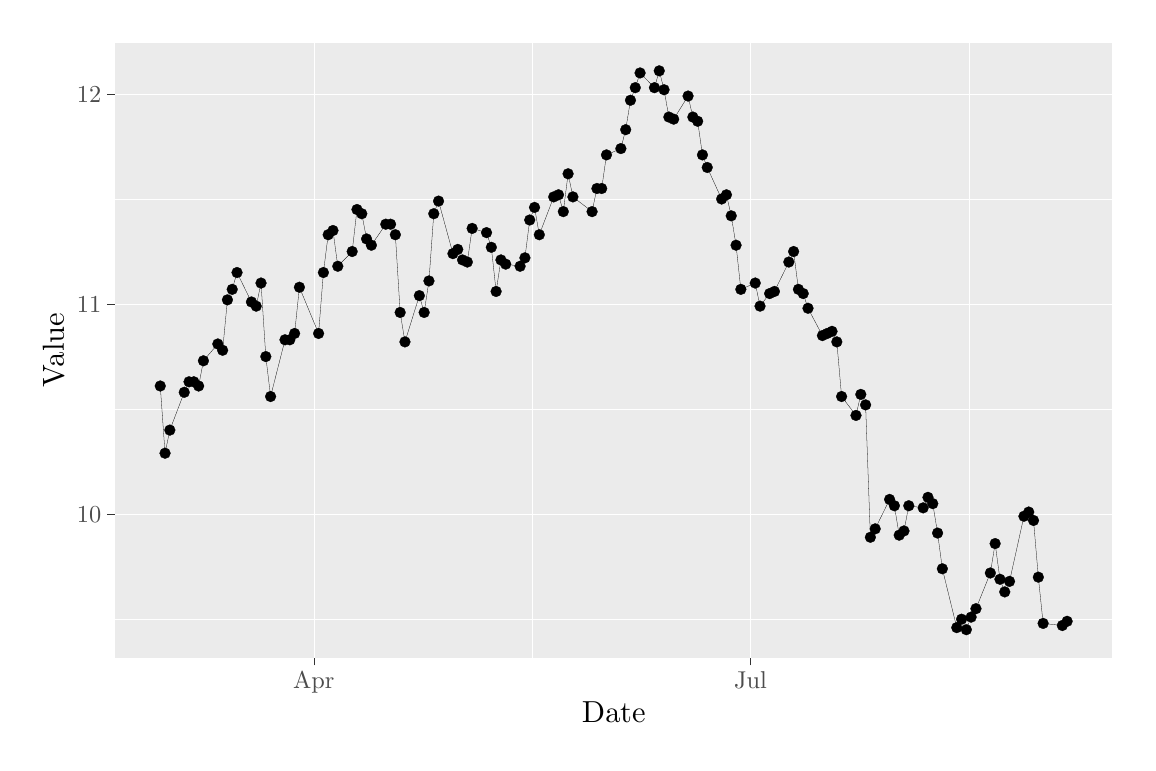
\begin{tikzpicture}[x=1pt,y=1pt]
\definecolor{fillColor}{RGB}{255,255,255}
\path[use as bounding box,fill=fillColor,fill opacity=0.00] (0,0) rectangle (397.48,258.37);
\begin{scope}
\path[clip] (  0.00,  0.00) rectangle (397.48,258.37);
\definecolor{drawColor}{RGB}{255,255,255}
\definecolor{fillColor}{RGB}{255,255,255}

\path[draw=drawColor,line width= 0.1pt,line join=round,line cap=round,fill=fillColor] (  0.00,  0.00) rectangle (397.48,258.37);
\end{scope}
\begin{scope}
\path[clip] ( 31.52, 30.73) rectangle (391.98,252.87);
\definecolor{fillColor}{gray}{0.92}

\path[fill=fillColor] ( 31.52, 30.73) rectangle (391.98,252.87);
\definecolor{drawColor}{RGB}{255,255,255}

\path[draw=drawColor,line width= 0.1pt,line join=round] ( 31.52, 44.62) --
	(391.98, 44.62);

\path[draw=drawColor,line width= 0.1pt,line join=round] ( 31.52,120.54) --
	(391.98,120.54);

\path[draw=drawColor,line width= 0.1pt,line join=round] ( 31.52,196.46) --
	(391.98,196.46);

\path[draw=drawColor,line width= 0.1pt,line join=round] (182.28, 30.73) --
	(182.28,252.87);

\path[draw=drawColor,line width= 0.1pt,line join=round] (340.06, 30.73) --
	(340.06,252.87);

\path[draw=drawColor,line width= 0.1pt,line join=round] ( 31.52, 82.58) --
	(391.98, 82.58);

\path[draw=drawColor,line width= 0.1pt,line join=round] ( 31.52,158.50) --
	(391.98,158.50);

\path[draw=drawColor,line width= 0.1pt,line join=round] ( 31.52,234.42) --
	(391.98,234.42);

\path[draw=drawColor,line width= 0.1pt,line join=round] (103.39, 30.73) --
	(103.39,252.87);

\path[draw=drawColor,line width= 0.1pt,line join=round] (261.17, 30.73) --
	(261.17,252.87);
\definecolor{drawColor}{RGB}{0,0,0}

\path[draw=drawColor,line width= 0.1pt,line join=round] ( 47.91,128.89) --
	( 49.64,104.60) --
	( 51.37,112.95) --
	( 56.58,126.61) --
	( 58.31,130.41) --
	( 60.04,130.41) --
	( 61.78,128.89) --
	( 63.51,138.00) --
	( 68.71,144.07) --
	( 70.45,141.80) --
	( 72.18,160.02) --
	( 73.91,163.81) --
	( 75.65,169.89) --
	( 80.85,159.26) --
	( 82.58,157.74) --
	( 84.32,166.09) --
	( 86.05,139.52) --
	( 87.78,125.09) --
	( 92.99,145.59) --
	( 94.72,145.59) --
	( 96.45,147.87) --
	( 98.19,164.57) --
	(105.12,147.87) --
	(106.86,169.89) --
	(108.59,183.55) --
	(110.32,185.07) --
	(112.06,172.16) --
	(117.26,177.48) --
	(118.99,192.66) --
	(120.73,191.14) --
	(122.46,182.03) --
	(124.20,179.76) --
	(129.40,187.35) --
	(131.13,187.35) --
	(132.86,183.55) --
	(134.60,155.46) --
	(136.33,144.83) --
	(141.53,161.54) --
	(143.27,155.46) --
	(145.00,166.85) --
	(146.74,191.14) --
	(148.47,195.70) --
	(153.67,176.72) --
	(155.40,178.24) --
	(157.14,174.44) --
	(158.87,173.68) --
	(160.61,185.83) --
	(165.81,184.31) --
	(167.54,179.00) --
	(169.27,163.05) --
	(171.01,174.44) --
	(172.74,172.92) --
	(177.94,172.16) --
	(179.68,175.20) --
	(181.41,188.87) --
	(183.15,193.42) --
	(184.88,183.55) --
	(190.08,197.22) --
	(191.81,197.98) --
	(193.55,191.90) --
	(195.28,205.57) --
	(197.02,197.22) --
	(203.95,191.90) --
	(205.69,200.25) --
	(207.42,200.25) --
	(209.15,212.40) --
	(214.35,214.68) --
	(216.09,221.51) --
	(217.82,232.14) --
	(219.56,236.69) --
	(221.29,242.01) --
	(226.49,236.69) --
	(228.22,242.77) --
	(229.96,235.94) --
	(231.69,226.07) --
	(233.43,225.31) --
	(238.63,233.66) --
	(240.36,226.07) --
	(242.10,224.55) --
	(243.83,212.40) --
	(245.56,207.85) --
	(250.76,196.46) --
	(252.50,197.98) --
	(254.23,190.38) --
	(255.97,179.76) --
	(257.70,163.81) --
	(262.90,166.09) --
	(264.64,157.74) --
	(268.10,162.29) --
	(269.84,163.05) --
	(275.04,173.68) --
	(276.77,177.48) --
	(278.51,163.81) --
	(280.24,162.29) --
	(281.97,156.98) --
	(287.18,147.11) --
	(288.91,147.87) --
	(290.64,148.63) --
	(292.38,144.83) --
	(294.11,125.09) --
	(299.31,118.26) --
	(301.05,125.85) --
	(302.78,122.06) --
	(304.51, 74.23) --
	(306.25, 77.27) --
	(311.45, 87.90) --
	(313.18, 85.62) --
	(314.92, 74.99) --
	(316.65, 76.51) --
	(318.38, 85.62) --
	(323.59, 84.86) --
	(325.32, 88.65) --
	(327.05, 86.38) --
	(328.79, 75.75) --
	(330.52, 62.84) --
	(335.72, 41.58) --
	(337.46, 44.62) --
	(339.19, 40.83) --
	(340.92, 45.38) --
	(342.66, 48.42) --
	(347.86, 61.32) --
	(349.59, 71.95) --
	(351.33, 59.05) --
	(353.06, 54.49) --
	(354.79, 58.29) --
	(360.00, 81.82) --
	(361.73, 83.34) --
	(363.46, 80.30) --
	(365.20, 59.81) --
	(366.93, 43.10) --
	(373.87, 42.34) --
	(375.60, 43.86);
\definecolor{fillColor}{RGB}{0,0,0}

\path[draw=drawColor,line width= 0.1pt,line join=round,line cap=round,fill=fillColor] ( 47.91,128.89) circle (  1.96);

\path[draw=drawColor,line width= 0.1pt,line join=round,line cap=round,fill=fillColor] ( 49.64,104.60) circle (  1.96);

\path[draw=drawColor,line width= 0.1pt,line join=round,line cap=round,fill=fillColor] ( 51.37,112.95) circle (  1.96);

\path[draw=drawColor,line width= 0.1pt,line join=round,line cap=round,fill=fillColor] ( 56.58,126.61) circle (  1.96);

\path[draw=drawColor,line width= 0.1pt,line join=round,line cap=round,fill=fillColor] ( 58.31,130.41) circle (  1.96);

\path[draw=drawColor,line width= 0.1pt,line join=round,line cap=round,fill=fillColor] ( 60.04,130.41) circle (  1.96);

\path[draw=drawColor,line width= 0.1pt,line join=round,line cap=round,fill=fillColor] ( 61.78,128.89) circle (  1.96);

\path[draw=drawColor,line width= 0.1pt,line join=round,line cap=round,fill=fillColor] ( 63.51,138.00) circle (  1.96);

\path[draw=drawColor,line width= 0.1pt,line join=round,line cap=round,fill=fillColor] ( 68.71,144.07) circle (  1.96);

\path[draw=drawColor,line width= 0.1pt,line join=round,line cap=round,fill=fillColor] ( 70.45,141.80) circle (  1.96);

\path[draw=drawColor,line width= 0.1pt,line join=round,line cap=round,fill=fillColor] ( 72.18,160.02) circle (  1.96);

\path[draw=drawColor,line width= 0.1pt,line join=round,line cap=round,fill=fillColor] ( 73.91,163.81) circle (  1.96);

\path[draw=drawColor,line width= 0.1pt,line join=round,line cap=round,fill=fillColor] ( 75.65,169.89) circle (  1.96);

\path[draw=drawColor,line width= 0.1pt,line join=round,line cap=round,fill=fillColor] ( 80.85,159.26) circle (  1.96);

\path[draw=drawColor,line width= 0.1pt,line join=round,line cap=round,fill=fillColor] ( 82.58,157.74) circle (  1.96);

\path[draw=drawColor,line width= 0.1pt,line join=round,line cap=round,fill=fillColor] ( 84.32,166.09) circle (  1.96);

\path[draw=drawColor,line width= 0.1pt,line join=round,line cap=round,fill=fillColor] ( 86.05,139.52) circle (  1.96);

\path[draw=drawColor,line width= 0.1pt,line join=round,line cap=round,fill=fillColor] ( 87.78,125.09) circle (  1.96);

\path[draw=drawColor,line width= 0.1pt,line join=round,line cap=round,fill=fillColor] ( 92.99,145.59) circle (  1.96);

\path[draw=drawColor,line width= 0.1pt,line join=round,line cap=round,fill=fillColor] ( 94.72,145.59) circle (  1.96);

\path[draw=drawColor,line width= 0.1pt,line join=round,line cap=round,fill=fillColor] ( 96.45,147.87) circle (  1.96);

\path[draw=drawColor,line width= 0.1pt,line join=round,line cap=round,fill=fillColor] ( 98.19,164.57) circle (  1.96);

\path[draw=drawColor,line width= 0.1pt,line join=round,line cap=round,fill=fillColor] (105.12,147.87) circle (  1.96);

\path[draw=drawColor,line width= 0.1pt,line join=round,line cap=round,fill=fillColor] (106.86,169.89) circle (  1.96);

\path[draw=drawColor,line width= 0.1pt,line join=round,line cap=round,fill=fillColor] (108.59,183.55) circle (  1.96);

\path[draw=drawColor,line width= 0.1pt,line join=round,line cap=round,fill=fillColor] (110.32,185.07) circle (  1.96);

\path[draw=drawColor,line width= 0.1pt,line join=round,line cap=round,fill=fillColor] (112.06,172.16) circle (  1.96);

\path[draw=drawColor,line width= 0.1pt,line join=round,line cap=round,fill=fillColor] (117.26,177.48) circle (  1.96);

\path[draw=drawColor,line width= 0.1pt,line join=round,line cap=round,fill=fillColor] (118.99,192.66) circle (  1.96);

\path[draw=drawColor,line width= 0.1pt,line join=round,line cap=round,fill=fillColor] (120.73,191.14) circle (  1.96);

\path[draw=drawColor,line width= 0.1pt,line join=round,line cap=round,fill=fillColor] (122.46,182.03) circle (  1.96);

\path[draw=drawColor,line width= 0.1pt,line join=round,line cap=round,fill=fillColor] (124.20,179.76) circle (  1.96);

\path[draw=drawColor,line width= 0.1pt,line join=round,line cap=round,fill=fillColor] (129.40,187.35) circle (  1.96);

\path[draw=drawColor,line width= 0.1pt,line join=round,line cap=round,fill=fillColor] (131.13,187.35) circle (  1.96);

\path[draw=drawColor,line width= 0.1pt,line join=round,line cap=round,fill=fillColor] (132.86,183.55) circle (  1.96);

\path[draw=drawColor,line width= 0.1pt,line join=round,line cap=round,fill=fillColor] (134.60,155.46) circle (  1.96);

\path[draw=drawColor,line width= 0.1pt,line join=round,line cap=round,fill=fillColor] (136.33,144.83) circle (  1.96);

\path[draw=drawColor,line width= 0.1pt,line join=round,line cap=round,fill=fillColor] (141.53,161.54) circle (  1.96);

\path[draw=drawColor,line width= 0.1pt,line join=round,line cap=round,fill=fillColor] (143.27,155.46) circle (  1.96);

\path[draw=drawColor,line width= 0.1pt,line join=round,line cap=round,fill=fillColor] (145.00,166.85) circle (  1.96);

\path[draw=drawColor,line width= 0.1pt,line join=round,line cap=round,fill=fillColor] (146.74,191.14) circle (  1.96);

\path[draw=drawColor,line width= 0.1pt,line join=round,line cap=round,fill=fillColor] (148.47,195.70) circle (  1.96);

\path[draw=drawColor,line width= 0.1pt,line join=round,line cap=round,fill=fillColor] (153.67,176.72) circle (  1.96);

\path[draw=drawColor,line width= 0.1pt,line join=round,line cap=round,fill=fillColor] (155.40,178.24) circle (  1.96);

\path[draw=drawColor,line width= 0.1pt,line join=round,line cap=round,fill=fillColor] (157.14,174.44) circle (  1.96);

\path[draw=drawColor,line width= 0.1pt,line join=round,line cap=round,fill=fillColor] (158.87,173.68) circle (  1.96);

\path[draw=drawColor,line width= 0.1pt,line join=round,line cap=round,fill=fillColor] (160.61,185.83) circle (  1.96);

\path[draw=drawColor,line width= 0.1pt,line join=round,line cap=round,fill=fillColor] (165.81,184.31) circle (  1.96);

\path[draw=drawColor,line width= 0.1pt,line join=round,line cap=round,fill=fillColor] (167.54,179.00) circle (  1.96);

\path[draw=drawColor,line width= 0.1pt,line join=round,line cap=round,fill=fillColor] (169.27,163.05) circle (  1.96);

\path[draw=drawColor,line width= 0.1pt,line join=round,line cap=round,fill=fillColor] (171.01,174.44) circle (  1.96);

\path[draw=drawColor,line width= 0.1pt,line join=round,line cap=round,fill=fillColor] (172.74,172.92) circle (  1.96);

\path[draw=drawColor,line width= 0.1pt,line join=round,line cap=round,fill=fillColor] (177.94,172.16) circle (  1.96);

\path[draw=drawColor,line width= 0.1pt,line join=round,line cap=round,fill=fillColor] (179.68,175.20) circle (  1.96);

\path[draw=drawColor,line width= 0.1pt,line join=round,line cap=round,fill=fillColor] (181.41,188.87) circle (  1.96);

\path[draw=drawColor,line width= 0.1pt,line join=round,line cap=round,fill=fillColor] (183.15,193.42) circle (  1.96);

\path[draw=drawColor,line width= 0.1pt,line join=round,line cap=round,fill=fillColor] (184.88,183.55) circle (  1.96);

\path[draw=drawColor,line width= 0.1pt,line join=round,line cap=round,fill=fillColor] (190.08,197.22) circle (  1.96);

\path[draw=drawColor,line width= 0.1pt,line join=round,line cap=round,fill=fillColor] (191.81,197.98) circle (  1.96);

\path[draw=drawColor,line width= 0.1pt,line join=round,line cap=round,fill=fillColor] (193.55,191.90) circle (  1.96);

\path[draw=drawColor,line width= 0.1pt,line join=round,line cap=round,fill=fillColor] (195.28,205.57) circle (  1.96);

\path[draw=drawColor,line width= 0.1pt,line join=round,line cap=round,fill=fillColor] (197.02,197.22) circle (  1.96);

\path[draw=drawColor,line width= 0.1pt,line join=round,line cap=round,fill=fillColor] (203.95,191.90) circle (  1.96);

\path[draw=drawColor,line width= 0.1pt,line join=round,line cap=round,fill=fillColor] (205.69,200.25) circle (  1.96);

\path[draw=drawColor,line width= 0.1pt,line join=round,line cap=round,fill=fillColor] (207.42,200.25) circle (  1.96);

\path[draw=drawColor,line width= 0.1pt,line join=round,line cap=round,fill=fillColor] (209.15,212.40) circle (  1.96);

\path[draw=drawColor,line width= 0.1pt,line join=round,line cap=round,fill=fillColor] (214.35,214.68) circle (  1.96);

\path[draw=drawColor,line width= 0.1pt,line join=round,line cap=round,fill=fillColor] (216.09,221.51) circle (  1.96);

\path[draw=drawColor,line width= 0.1pt,line join=round,line cap=round,fill=fillColor] (217.82,232.14) circle (  1.96);

\path[draw=drawColor,line width= 0.1pt,line join=round,line cap=round,fill=fillColor] (219.56,236.69) circle (  1.96);

\path[draw=drawColor,line width= 0.1pt,line join=round,line cap=round,fill=fillColor] (221.29,242.01) circle (  1.96);

\path[draw=drawColor,line width= 0.1pt,line join=round,line cap=round,fill=fillColor] (226.49,236.69) circle (  1.96);

\path[draw=drawColor,line width= 0.1pt,line join=round,line cap=round,fill=fillColor] (228.22,242.77) circle (  1.96);

\path[draw=drawColor,line width= 0.1pt,line join=round,line cap=round,fill=fillColor] (229.96,235.94) circle (  1.96);

\path[draw=drawColor,line width= 0.1pt,line join=round,line cap=round,fill=fillColor] (231.69,226.07) circle (  1.96);

\path[draw=drawColor,line width= 0.1pt,line join=round,line cap=round,fill=fillColor] (233.43,225.31) circle (  1.96);

\path[draw=drawColor,line width= 0.1pt,line join=round,line cap=round,fill=fillColor] (238.63,233.66) circle (  1.96);

\path[draw=drawColor,line width= 0.1pt,line join=round,line cap=round,fill=fillColor] (240.36,226.07) circle (  1.96);

\path[draw=drawColor,line width= 0.1pt,line join=round,line cap=round,fill=fillColor] (242.10,224.55) circle (  1.96);

\path[draw=drawColor,line width= 0.1pt,line join=round,line cap=round,fill=fillColor] (243.83,212.40) circle (  1.96);

\path[draw=drawColor,line width= 0.1pt,line join=round,line cap=round,fill=fillColor] (245.56,207.85) circle (  1.96);

\path[draw=drawColor,line width= 0.1pt,line join=round,line cap=round,fill=fillColor] (250.76,196.46) circle (  1.96);

\path[draw=drawColor,line width= 0.1pt,line join=round,line cap=round,fill=fillColor] (252.50,197.98) circle (  1.96);

\path[draw=drawColor,line width= 0.1pt,line join=round,line cap=round,fill=fillColor] (254.23,190.38) circle (  1.96);

\path[draw=drawColor,line width= 0.1pt,line join=round,line cap=round,fill=fillColor] (255.97,179.76) circle (  1.96);

\path[draw=drawColor,line width= 0.1pt,line join=round,line cap=round,fill=fillColor] (257.70,163.81) circle (  1.96);

\path[draw=drawColor,line width= 0.1pt,line join=round,line cap=round,fill=fillColor] (262.90,166.09) circle (  1.96);

\path[draw=drawColor,line width= 0.1pt,line join=round,line cap=round,fill=fillColor] (264.64,157.74) circle (  1.96);

\path[draw=drawColor,line width= 0.1pt,line join=round,line cap=round,fill=fillColor] (268.10,162.29) circle (  1.96);

\path[draw=drawColor,line width= 0.1pt,line join=round,line cap=round,fill=fillColor] (269.84,163.05) circle (  1.96);

\path[draw=drawColor,line width= 0.1pt,line join=round,line cap=round,fill=fillColor] (275.04,173.68) circle (  1.96);

\path[draw=drawColor,line width= 0.1pt,line join=round,line cap=round,fill=fillColor] (276.77,177.48) circle (  1.96);

\path[draw=drawColor,line width= 0.1pt,line join=round,line cap=round,fill=fillColor] (278.51,163.81) circle (  1.96);

\path[draw=drawColor,line width= 0.1pt,line join=round,line cap=round,fill=fillColor] (280.24,162.29) circle (  1.96);

\path[draw=drawColor,line width= 0.1pt,line join=round,line cap=round,fill=fillColor] (281.97,156.98) circle (  1.96);

\path[draw=drawColor,line width= 0.1pt,line join=round,line cap=round,fill=fillColor] (287.18,147.11) circle (  1.96);

\path[draw=drawColor,line width= 0.1pt,line join=round,line cap=round,fill=fillColor] (288.91,147.87) circle (  1.96);

\path[draw=drawColor,line width= 0.1pt,line join=round,line cap=round,fill=fillColor] (290.64,148.63) circle (  1.96);

\path[draw=drawColor,line width= 0.1pt,line join=round,line cap=round,fill=fillColor] (292.38,144.83) circle (  1.96);

\path[draw=drawColor,line width= 0.1pt,line join=round,line cap=round,fill=fillColor] (294.11,125.09) circle (  1.96);

\path[draw=drawColor,line width= 0.1pt,line join=round,line cap=round,fill=fillColor] (299.31,118.26) circle (  1.96);

\path[draw=drawColor,line width= 0.1pt,line join=round,line cap=round,fill=fillColor] (301.05,125.85) circle (  1.96);

\path[draw=drawColor,line width= 0.1pt,line join=round,line cap=round,fill=fillColor] (302.78,122.06) circle (  1.96);

\path[draw=drawColor,line width= 0.1pt,line join=round,line cap=round,fill=fillColor] (304.51, 74.23) circle (  1.96);

\path[draw=drawColor,line width= 0.1pt,line join=round,line cap=round,fill=fillColor] (306.25, 77.27) circle (  1.96);

\path[draw=drawColor,line width= 0.1pt,line join=round,line cap=round,fill=fillColor] (311.45, 87.90) circle (  1.96);

\path[draw=drawColor,line width= 0.1pt,line join=round,line cap=round,fill=fillColor] (313.18, 85.62) circle (  1.96);

\path[draw=drawColor,line width= 0.1pt,line join=round,line cap=round,fill=fillColor] (314.92, 74.99) circle (  1.96);

\path[draw=drawColor,line width= 0.1pt,line join=round,line cap=round,fill=fillColor] (316.65, 76.51) circle (  1.96);

\path[draw=drawColor,line width= 0.1pt,line join=round,line cap=round,fill=fillColor] (318.38, 85.62) circle (  1.96);

\path[draw=drawColor,line width= 0.1pt,line join=round,line cap=round,fill=fillColor] (323.59, 84.86) circle (  1.96);

\path[draw=drawColor,line width= 0.1pt,line join=round,line cap=round,fill=fillColor] (325.32, 88.65) circle (  1.96);

\path[draw=drawColor,line width= 0.1pt,line join=round,line cap=round,fill=fillColor] (327.05, 86.38) circle (  1.96);

\path[draw=drawColor,line width= 0.1pt,line join=round,line cap=round,fill=fillColor] (328.79, 75.75) circle (  1.96);

\path[draw=drawColor,line width= 0.1pt,line join=round,line cap=round,fill=fillColor] (330.52, 62.84) circle (  1.96);

\path[draw=drawColor,line width= 0.1pt,line join=round,line cap=round,fill=fillColor] (335.72, 41.58) circle (  1.96);

\path[draw=drawColor,line width= 0.1pt,line join=round,line cap=round,fill=fillColor] (337.46, 44.62) circle (  1.96);

\path[draw=drawColor,line width= 0.1pt,line join=round,line cap=round,fill=fillColor] (339.19, 40.83) circle (  1.96);

\path[draw=drawColor,line width= 0.1pt,line join=round,line cap=round,fill=fillColor] (340.92, 45.38) circle (  1.96);

\path[draw=drawColor,line width= 0.1pt,line join=round,line cap=round,fill=fillColor] (342.66, 48.42) circle (  1.96);

\path[draw=drawColor,line width= 0.1pt,line join=round,line cap=round,fill=fillColor] (347.86, 61.32) circle (  1.96);

\path[draw=drawColor,line width= 0.1pt,line join=round,line cap=round,fill=fillColor] (349.59, 71.95) circle (  1.96);

\path[draw=drawColor,line width= 0.1pt,line join=round,line cap=round,fill=fillColor] (351.33, 59.05) circle (  1.96);

\path[draw=drawColor,line width= 0.1pt,line join=round,line cap=round,fill=fillColor] (353.06, 54.49) circle (  1.96);

\path[draw=drawColor,line width= 0.1pt,line join=round,line cap=round,fill=fillColor] (354.79, 58.29) circle (  1.96);

\path[draw=drawColor,line width= 0.1pt,line join=round,line cap=round,fill=fillColor] (360.00, 81.82) circle (  1.96);

\path[draw=drawColor,line width= 0.1pt,line join=round,line cap=round,fill=fillColor] (361.73, 83.34) circle (  1.96);

\path[draw=drawColor,line width= 0.1pt,line join=round,line cap=round,fill=fillColor] (363.46, 80.30) circle (  1.96);

\path[draw=drawColor,line width= 0.1pt,line join=round,line cap=round,fill=fillColor] (365.20, 59.81) circle (  1.96);

\path[draw=drawColor,line width= 0.1pt,line join=round,line cap=round,fill=fillColor] (366.93, 43.10) circle (  1.96);

\path[draw=drawColor,line width= 0.1pt,line join=round,line cap=round,fill=fillColor] (373.87, 42.34) circle (  1.96);

\path[draw=drawColor,line width= 0.1pt,line join=round,line cap=round,fill=fillColor] (375.60, 43.86) circle (  1.96);
\end{scope}
\begin{scope}
\path[clip] (  0.00,  0.00) rectangle (397.48,258.37);
\definecolor{drawColor}{gray}{0.30}

\node[text=drawColor,anchor=base east,inner sep=0pt, outer sep=0pt, scale=  0.88] at ( 26.57, 79.55) {10};

\node[text=drawColor,anchor=base east,inner sep=0pt, outer sep=0pt, scale=  0.88] at ( 26.57,155.47) {11};

\node[text=drawColor,anchor=base east,inner sep=0pt, outer sep=0pt, scale=  0.88] at ( 26.57,231.39) {12};
\end{scope}
\begin{scope}
\path[clip] (  0.00,  0.00) rectangle (397.48,258.37);
\definecolor{drawColor}{gray}{0.20}

\path[draw=drawColor,line width= 0.1pt,line join=round] ( 28.77, 82.58) --
	( 31.52, 82.58);

\path[draw=drawColor,line width= 0.1pt,line join=round] ( 28.77,158.50) --
	( 31.52,158.50);

\path[draw=drawColor,line width= 0.1pt,line join=round] ( 28.77,234.42) --
	( 31.52,234.42);
\end{scope}
\begin{scope}
\path[clip] (  0.00,  0.00) rectangle (397.48,258.37);
\definecolor{drawColor}{gray}{0.20}

\path[draw=drawColor,line width= 0.1pt,line join=round] (103.39, 27.98) --
	(103.39, 30.73);

\path[draw=drawColor,line width= 0.1pt,line join=round] (261.17, 27.98) --
	(261.17, 30.73);
\end{scope}
\begin{scope}
\path[clip] (  0.00,  0.00) rectangle (397.48,258.37);
\definecolor{drawColor}{gray}{0.30}

\node[text=drawColor,anchor=base,inner sep=0pt, outer sep=0pt, scale=  0.88] at (103.39, 19.72) {Apr};

\node[text=drawColor,anchor=base,inner sep=0pt, outer sep=0pt, scale=  0.88] at (261.17, 19.72) {Jul};
\end{scope}
\begin{scope}
\path[clip] (  0.00,  0.00) rectangle (397.48,258.37);
\definecolor{drawColor}{RGB}{0,0,0}

\node[text=drawColor,anchor=base,inner sep=0pt, outer sep=0pt, scale=  1.10] at (211.75,  7.44) {Date};
\end{scope}
\begin{scope}
\path[clip] (  0.00,  0.00) rectangle (397.48,258.37);
\definecolor{drawColor}{RGB}{0,0,0}

\node[text=drawColor,rotate= 90.00,anchor=base,inner sep=0pt, outer sep=0pt, scale=  1.10] at ( 13.08,141.80) {Value};
\end{scope}
\end{tikzpicture}

    \caption{\indicesCaption{\ford}}
    \label{fig:analysis-indices-ford}
\end{figure}    

\subsection{\gm}
\label{ss:analysis-datasets-gm}

% From         To Days Tweets
% DG#0  2018-06-26 2018-08-01   37 270276
% DG#1  2018-08-20 2018-09-06   18 143541
% Total 2018-06-26 2018-09-06   55 413817

For the \gm\ \num{413817} english tweets have been captured in total between \printdate{2018-06-26} and \printdate{2018-09-06}.
But as stated earlier in \cref{ss:casestudy-gatherdata-tweets} this was not a continuous time frame.
The various collected time frames, number of consecutive days in each frame and collected tweets in that frame are depicted in \cref{tab:anaylsis-datasets-gm}.

\begin{table}[hbt]
    \centering
    \begin{tabular}{!>{\bfseries}l ^l ^l ^r ^r}
      \hline
      \rowstyle{\bfseries}
                & From & To & \# Days & \# Tweets \\ \hline
        Group 1 & \printdate{2018-06-26} & \printdate{2018-08-01} &   \num{37} & \num{270276} \\
        Group 2 & \printdate{2018-08-20} & \printdate{2018-09-06} &   \num{18} & \num{143541} \\ \hline
        Total   & \printdate{2018-06-26} & \printdate{2018-09-06} &   \num{99} & \num{413817} \\ \hline
    \end{tabular}
  
    \caption{\tweetsCaption{\gm}}
    \label{tab:anaylsis-datasets-gm}
\end{table}

Therefore, share prices have been downloaded for the entire given time frame which is depicted in \cref{fig:analysis-indices-gm}.

\begin{figure}[hbt]
    \centering
    % Created by tikzDevice version 0.12 on 2019-02-27 16:25:31
% !TEX encoding = UTF-8 Unicode
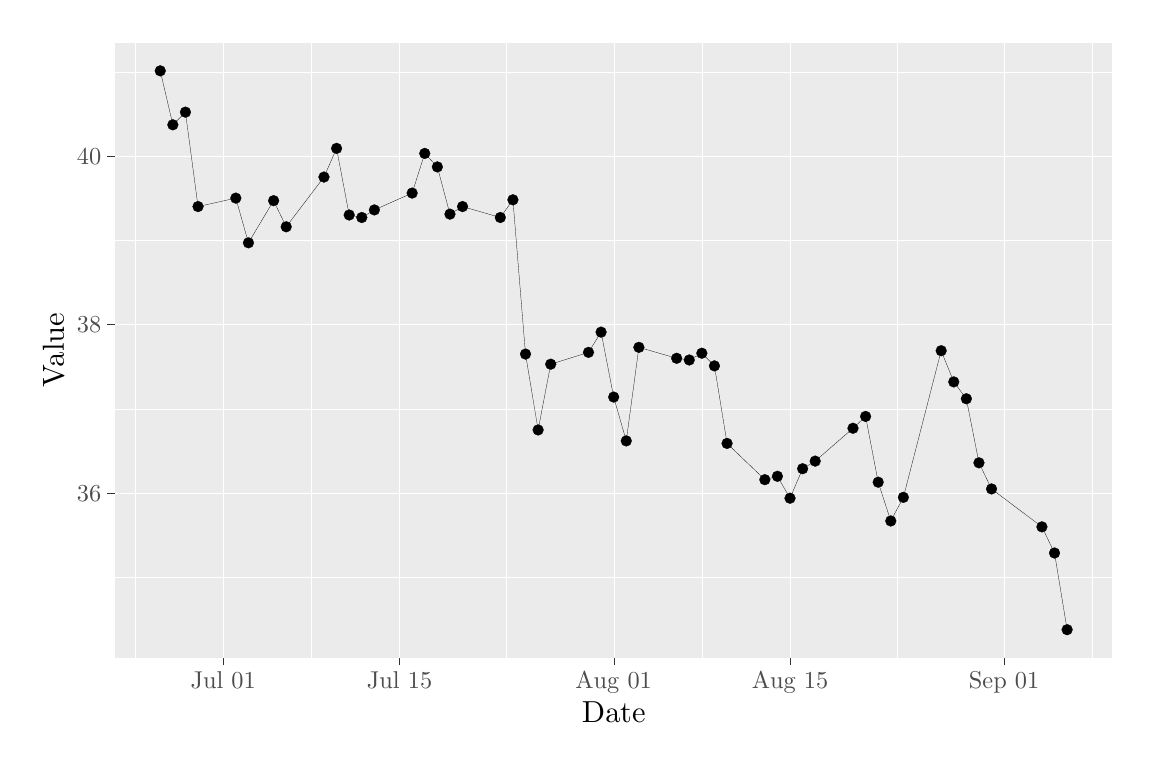
\begin{tikzpicture}[x=1pt,y=1pt]
\definecolor{fillColor}{RGB}{255,255,255}
\path[use as bounding box,fill=fillColor,fill opacity=0.00] (0,0) rectangle (397.48,258.37);
\begin{scope}
\path[clip] (  0.00,  0.00) rectangle (397.48,258.37);
\definecolor{drawColor}{RGB}{255,255,255}
\definecolor{fillColor}{RGB}{255,255,255}

\path[draw=drawColor,line width= 0.1pt,line join=round,line cap=round,fill=fillColor] (  0.00,  0.00) rectangle (397.48,258.37);
\end{scope}
\begin{scope}
\path[clip] ( 31.52, 30.73) rectangle (391.98,252.87);
\definecolor{fillColor}{gray}{0.92}

\path[fill=fillColor] ( 31.52, 30.73) rectangle (391.98,252.87);
\definecolor{drawColor}{RGB}{255,255,255}

\path[draw=drawColor,line width= 0.1pt,line join=round] ( 31.52, 59.71) --
	(391.98, 59.71);

\path[draw=drawColor,line width= 0.1pt,line join=round] ( 31.52,120.63) --
	(391.98,120.63);

\path[draw=drawColor,line width= 0.1pt,line join=round] ( 31.52,181.55) --
	(391.98,181.55);

\path[draw=drawColor,line width= 0.1pt,line join=round] ( 31.52,242.46) --
	(391.98,242.46);

\path[draw=drawColor,line width= 0.1pt,line join=round] ( 38.80, 30.73) --
	( 38.80,252.87);

\path[draw=drawColor,line width= 0.1pt,line join=round] (102.52, 30.73) --
	(102.52,252.87);

\path[draw=drawColor,line width= 0.1pt,line join=round] (173.07, 30.73) --
	(173.07,252.87);

\path[draw=drawColor,line width= 0.1pt,line join=round] (243.61, 30.73) --
	(243.61,252.87);

\path[draw=drawColor,line width= 0.1pt,line join=round] (314.16, 30.73) --
	(314.16,252.87);

\path[draw=drawColor,line width= 0.1pt,line join=round] (384.70, 30.73) --
	(384.70,252.87);

\path[draw=drawColor,line width= 0.1pt,line join=round] ( 31.52, 90.17) --
	(391.98, 90.17);

\path[draw=drawColor,line width= 0.1pt,line join=round] ( 31.52,151.09) --
	(391.98,151.09);

\path[draw=drawColor,line width= 0.1pt,line join=round] ( 31.52,212.00) --
	(391.98,212.00);

\path[draw=drawColor,line width= 0.1pt,line join=round] ( 70.66, 30.73) --
	( 70.66,252.87);

\path[draw=drawColor,line width= 0.1pt,line join=round] (134.38, 30.73) --
	(134.38,252.87);

\path[draw=drawColor,line width= 0.1pt,line join=round] (211.75, 30.73) --
	(211.75,252.87);

\path[draw=drawColor,line width= 0.1pt,line join=round] (275.47, 30.73) --
	(275.47,252.87);

\path[draw=drawColor,line width= 0.1pt,line join=round] (352.84, 30.73) --
	(352.84,252.87);
\definecolor{drawColor}{RGB}{0,0,0}

\path[draw=drawColor,line width= 0.1pt,line join=round] ( 47.91,242.77) --
	( 52.46,223.27) --
	( 57.01,227.84) --
	( 61.56,193.73) --
	( 75.21,196.78) --
	( 79.77,180.63) --
	( 88.87,195.86) --
	( 93.42,186.42) --
	(107.07,204.39) --
	(111.62,214.75) --
	(116.18,190.68) --
	(120.73,189.77) --
	(125.28,192.51) --
	(138.93,198.60) --
	(143.48,212.92) --
	(148.04,208.05) --
	(152.59,190.99) --
	(157.14,193.73) --
	(170.79,189.77) --
	(175.34,196.17) --
	(179.89,140.43) --
	(184.45,113.01) --
	(189.00,136.77) --
	(202.65,141.04) --
	(207.20,148.35) --
	(211.75,124.89) --
	(216.30,109.05) --
	(220.86,142.86) --
	(234.51,138.90) --
	(239.06,138.29) --
	(243.61,140.73) --
	(248.16,136.16) --
	(252.72,108.14) --
	(266.37, 95.04) --
	(270.92, 96.26) --
	(275.47, 88.34) --
	(280.02, 99.00) --
	(284.57,101.74) --
	(298.23,113.62) --
	(302.78,117.89) --
	(307.33, 94.13) --
	(311.88, 80.12) --
	(316.43, 88.65) --
	(330.09,141.64) --
	(334.64,130.37) --
	(339.19,124.28) --
	(343.74,101.13) --
	(348.29, 91.69) --
	(366.50, 77.99) --
	(371.05, 68.54) --
	(375.60, 40.83);
\definecolor{fillColor}{RGB}{0,0,0}

\path[draw=drawColor,line width= 0.1pt,line join=round,line cap=round,fill=fillColor] ( 47.91,242.77) circle (  1.96);

\path[draw=drawColor,line width= 0.1pt,line join=round,line cap=round,fill=fillColor] ( 52.46,223.27) circle (  1.96);

\path[draw=drawColor,line width= 0.1pt,line join=round,line cap=round,fill=fillColor] ( 57.01,227.84) circle (  1.96);

\path[draw=drawColor,line width= 0.1pt,line join=round,line cap=round,fill=fillColor] ( 61.56,193.73) circle (  1.96);

\path[draw=drawColor,line width= 0.1pt,line join=round,line cap=round,fill=fillColor] ( 75.21,196.78) circle (  1.96);

\path[draw=drawColor,line width= 0.1pt,line join=round,line cap=round,fill=fillColor] ( 79.77,180.63) circle (  1.96);

\path[draw=drawColor,line width= 0.1pt,line join=round,line cap=round,fill=fillColor] ( 88.87,195.86) circle (  1.96);

\path[draw=drawColor,line width= 0.1pt,line join=round,line cap=round,fill=fillColor] ( 93.42,186.42) circle (  1.96);

\path[draw=drawColor,line width= 0.1pt,line join=round,line cap=round,fill=fillColor] (107.07,204.39) circle (  1.96);

\path[draw=drawColor,line width= 0.1pt,line join=round,line cap=round,fill=fillColor] (111.62,214.75) circle (  1.96);

\path[draw=drawColor,line width= 0.1pt,line join=round,line cap=round,fill=fillColor] (116.18,190.68) circle (  1.96);

\path[draw=drawColor,line width= 0.1pt,line join=round,line cap=round,fill=fillColor] (120.73,189.77) circle (  1.96);

\path[draw=drawColor,line width= 0.1pt,line join=round,line cap=round,fill=fillColor] (125.28,192.51) circle (  1.96);

\path[draw=drawColor,line width= 0.1pt,line join=round,line cap=round,fill=fillColor] (138.93,198.60) circle (  1.96);

\path[draw=drawColor,line width= 0.1pt,line join=round,line cap=round,fill=fillColor] (143.48,212.92) circle (  1.96);

\path[draw=drawColor,line width= 0.1pt,line join=round,line cap=round,fill=fillColor] (148.04,208.05) circle (  1.96);

\path[draw=drawColor,line width= 0.1pt,line join=round,line cap=round,fill=fillColor] (152.59,190.99) circle (  1.96);

\path[draw=drawColor,line width= 0.1pt,line join=round,line cap=round,fill=fillColor] (157.14,193.73) circle (  1.96);

\path[draw=drawColor,line width= 0.1pt,line join=round,line cap=round,fill=fillColor] (170.79,189.77) circle (  1.96);

\path[draw=drawColor,line width= 0.1pt,line join=round,line cap=round,fill=fillColor] (175.34,196.17) circle (  1.96);

\path[draw=drawColor,line width= 0.1pt,line join=round,line cap=round,fill=fillColor] (179.89,140.43) circle (  1.96);

\path[draw=drawColor,line width= 0.1pt,line join=round,line cap=round,fill=fillColor] (184.45,113.01) circle (  1.96);

\path[draw=drawColor,line width= 0.1pt,line join=round,line cap=round,fill=fillColor] (189.00,136.77) circle (  1.96);

\path[draw=drawColor,line width= 0.1pt,line join=round,line cap=round,fill=fillColor] (202.65,141.04) circle (  1.96);

\path[draw=drawColor,line width= 0.1pt,line join=round,line cap=round,fill=fillColor] (207.20,148.35) circle (  1.96);

\path[draw=drawColor,line width= 0.1pt,line join=round,line cap=round,fill=fillColor] (211.75,124.89) circle (  1.96);

\path[draw=drawColor,line width= 0.1pt,line join=round,line cap=round,fill=fillColor] (216.30,109.05) circle (  1.96);

\path[draw=drawColor,line width= 0.1pt,line join=round,line cap=round,fill=fillColor] (220.86,142.86) circle (  1.96);

\path[draw=drawColor,line width= 0.1pt,line join=round,line cap=round,fill=fillColor] (234.51,138.90) circle (  1.96);

\path[draw=drawColor,line width= 0.1pt,line join=round,line cap=round,fill=fillColor] (239.06,138.29) circle (  1.96);

\path[draw=drawColor,line width= 0.1pt,line join=round,line cap=round,fill=fillColor] (243.61,140.73) circle (  1.96);

\path[draw=drawColor,line width= 0.1pt,line join=round,line cap=round,fill=fillColor] (248.16,136.16) circle (  1.96);

\path[draw=drawColor,line width= 0.1pt,line join=round,line cap=round,fill=fillColor] (252.72,108.14) circle (  1.96);

\path[draw=drawColor,line width= 0.1pt,line join=round,line cap=round,fill=fillColor] (266.37, 95.04) circle (  1.96);

\path[draw=drawColor,line width= 0.1pt,line join=round,line cap=round,fill=fillColor] (270.92, 96.26) circle (  1.96);

\path[draw=drawColor,line width= 0.1pt,line join=round,line cap=round,fill=fillColor] (275.47, 88.34) circle (  1.96);

\path[draw=drawColor,line width= 0.1pt,line join=round,line cap=round,fill=fillColor] (280.02, 99.00) circle (  1.96);

\path[draw=drawColor,line width= 0.1pt,line join=round,line cap=round,fill=fillColor] (284.57,101.74) circle (  1.96);

\path[draw=drawColor,line width= 0.1pt,line join=round,line cap=round,fill=fillColor] (298.23,113.62) circle (  1.96);

\path[draw=drawColor,line width= 0.1pt,line join=round,line cap=round,fill=fillColor] (302.78,117.89) circle (  1.96);

\path[draw=drawColor,line width= 0.1pt,line join=round,line cap=round,fill=fillColor] (307.33, 94.13) circle (  1.96);

\path[draw=drawColor,line width= 0.1pt,line join=round,line cap=round,fill=fillColor] (311.88, 80.12) circle (  1.96);

\path[draw=drawColor,line width= 0.1pt,line join=round,line cap=round,fill=fillColor] (316.43, 88.65) circle (  1.96);

\path[draw=drawColor,line width= 0.1pt,line join=round,line cap=round,fill=fillColor] (330.09,141.64) circle (  1.96);

\path[draw=drawColor,line width= 0.1pt,line join=round,line cap=round,fill=fillColor] (334.64,130.37) circle (  1.96);

\path[draw=drawColor,line width= 0.1pt,line join=round,line cap=round,fill=fillColor] (339.19,124.28) circle (  1.96);

\path[draw=drawColor,line width= 0.1pt,line join=round,line cap=round,fill=fillColor] (343.74,101.13) circle (  1.96);

\path[draw=drawColor,line width= 0.1pt,line join=round,line cap=round,fill=fillColor] (348.29, 91.69) circle (  1.96);

\path[draw=drawColor,line width= 0.1pt,line join=round,line cap=round,fill=fillColor] (366.50, 77.99) circle (  1.96);

\path[draw=drawColor,line width= 0.1pt,line join=round,line cap=round,fill=fillColor] (371.05, 68.54) circle (  1.96);

\path[draw=drawColor,line width= 0.1pt,line join=round,line cap=round,fill=fillColor] (375.60, 40.83) circle (  1.96);
\end{scope}
\begin{scope}
\path[clip] (  0.00,  0.00) rectangle (397.48,258.37);
\definecolor{drawColor}{gray}{0.30}

\node[text=drawColor,anchor=base east,inner sep=0pt, outer sep=0pt, scale=  0.88] at ( 26.57, 87.14) {36};

\node[text=drawColor,anchor=base east,inner sep=0pt, outer sep=0pt, scale=  0.88] at ( 26.57,148.06) {38};

\node[text=drawColor,anchor=base east,inner sep=0pt, outer sep=0pt, scale=  0.88] at ( 26.57,208.97) {40};
\end{scope}
\begin{scope}
\path[clip] (  0.00,  0.00) rectangle (397.48,258.37);
\definecolor{drawColor}{gray}{0.20}

\path[draw=drawColor,line width= 0.1pt,line join=round] ( 28.77, 90.17) --
	( 31.52, 90.17);

\path[draw=drawColor,line width= 0.1pt,line join=round] ( 28.77,151.09) --
	( 31.52,151.09);

\path[draw=drawColor,line width= 0.1pt,line join=round] ( 28.77,212.00) --
	( 31.52,212.00);
\end{scope}
\begin{scope}
\path[clip] (  0.00,  0.00) rectangle (397.48,258.37);
\definecolor{drawColor}{gray}{0.20}

\path[draw=drawColor,line width= 0.1pt,line join=round] ( 70.66, 27.98) --
	( 70.66, 30.73);

\path[draw=drawColor,line width= 0.1pt,line join=round] (134.38, 27.98) --
	(134.38, 30.73);

\path[draw=drawColor,line width= 0.1pt,line join=round] (211.75, 27.98) --
	(211.75, 30.73);

\path[draw=drawColor,line width= 0.1pt,line join=round] (275.47, 27.98) --
	(275.47, 30.73);

\path[draw=drawColor,line width= 0.1pt,line join=round] (352.84, 27.98) --
	(352.84, 30.73);
\end{scope}
\begin{scope}
\path[clip] (  0.00,  0.00) rectangle (397.48,258.37);
\definecolor{drawColor}{gray}{0.30}

\node[text=drawColor,anchor=base,inner sep=0pt, outer sep=0pt, scale=  0.88] at ( 70.66, 19.72) {Jul 01};

\node[text=drawColor,anchor=base,inner sep=0pt, outer sep=0pt, scale=  0.88] at (134.38, 19.72) {Jul 15};

\node[text=drawColor,anchor=base,inner sep=0pt, outer sep=0pt, scale=  0.88] at (211.75, 19.72) {Aug 01};

\node[text=drawColor,anchor=base,inner sep=0pt, outer sep=0pt, scale=  0.88] at (275.47, 19.72) {Aug 15};

\node[text=drawColor,anchor=base,inner sep=0pt, outer sep=0pt, scale=  0.88] at (352.84, 19.72) {Sep 01};
\end{scope}
\begin{scope}
\path[clip] (  0.00,  0.00) rectangle (397.48,258.37);
\definecolor{drawColor}{RGB}{0,0,0}

\node[text=drawColor,anchor=base,inner sep=0pt, outer sep=0pt, scale=  1.10] at (211.75,  7.44) {Date};
\end{scope}
\begin{scope}
\path[clip] (  0.00,  0.00) rectangle (397.48,258.37);
\definecolor{drawColor}{RGB}{0,0,0}

\node[text=drawColor,rotate= 90.00,anchor=base,inner sep=0pt, outer sep=0pt, scale=  1.10] at ( 13.08,141.80) {Value};
\end{scope}
\end{tikzpicture}

    \caption{\indicesCaption{\gm}}
    \label{fig:analysis-indices-gm}
\end{figure}   

\subsection{\hyundai}
\label{ss:analysis-datasets-hyundai}

% From         To Days Tweets
% DG#0  2018-02-28 2018-04-08   40 363840
% DG#4  2018-06-26 2018-08-01   37 232092
% DG#5  2018-08-20 2018-09-07   19 101289
% Total 2018-02-28 2018-09-07   96 697221

For the \hyundai\ \num{697221} english tweets have been captured in total between \printdate{2018-02-28} and \printdate{2018-09-07}.
But as stated earlier in \cref{ss:casestudy-gatherdata-tweets} this was not a continuous time frame.
The various collected time frames, number of consecutive days in each frame and collected tweets in that frame are depicted in \cref{tab:anaylsis-datasets-hyundai}.

\begin{table}[hbt]
    \centering
    \begin{tabular}{!>{\bfseries}l ^l ^l ^r ^r}
      \hline
      \rowstyle{\bfseries}
                & From & To & \# Days & \# Tweets \\ \hline
        Group 1 & \printdate{2018-02-28} & \printdate{2018-04-08} &   \num{40} & \num{363840} \\
        Group 2 & \printdate{2018-06-26} & \printdate{2018-08-01} &   \num{37} & \num{232092} \\
        Group 3 & \printdate{2018-08-20} & \printdate{2018-09-07} &   \num{19} & \num{101289} \\ \hline
        Total   & \printdate{2018-02-28} & \printdate{2018-09-07} &   \num{96} & \num{697221} \\ \hline
    \end{tabular}
  
    \caption{\tweetsCaption{\hyundai}}
    \label{tab:anaylsis-datasets-hyundai}
\end{table}

Therefore, share prices have been downloaded for the entire given time frame which is depicted in \cref{fig:analysis-indices-hyundai}.

\begin{figure}[hbt]
    \centering
    % Created by tikzDevice version 0.12 on 2019-02-27 16:25:30
% !TEX encoding = UTF-8 Unicode
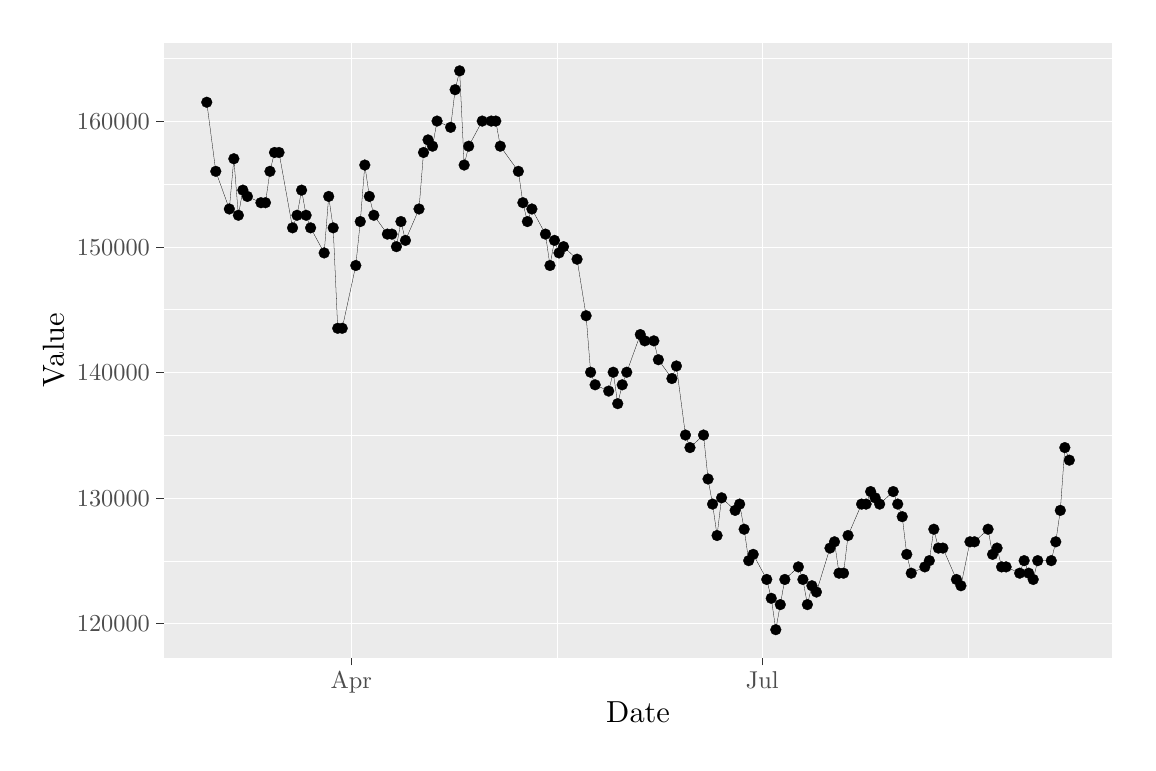
\begin{tikzpicture}[x=1pt,y=1pt]
\definecolor{fillColor}{RGB}{255,255,255}
\path[use as bounding box,fill=fillColor,fill opacity=0.00] (0,0) rectangle (397.48,258.37);
\begin{scope}
\path[clip] (  0.00,  0.00) rectangle (397.48,258.37);
\definecolor{drawColor}{RGB}{255,255,255}
\definecolor{fillColor}{RGB}{255,255,255}

\path[draw=drawColor,line width= 0.1pt,line join=round,line cap=round,fill=fillColor] (  0.00,  0.00) rectangle (397.48,258.37);
\end{scope}
\begin{scope}
\path[clip] ( 49.12, 30.73) rectangle (391.98,252.87);
\definecolor{fillColor}{gray}{0.92}

\path[fill=fillColor] ( 49.12, 30.73) rectangle (391.98,252.87);
\definecolor{drawColor}{RGB}{255,255,255}

\path[draw=drawColor,line width= 0.1pt,line join=round] ( 49.12, 65.78) --
	(391.98, 65.78);

\path[draw=drawColor,line width= 0.1pt,line join=round] ( 49.12,111.17) --
	(391.98,111.17);

\path[draw=drawColor,line width= 0.1pt,line join=round] ( 49.12,156.55) --
	(391.98,156.55);

\path[draw=drawColor,line width= 0.1pt,line join=round] ( 49.12,201.93) --
	(391.98,201.93);

\path[draw=drawColor,line width= 0.1pt,line join=round] ( 49.12,247.31) --
	(391.98,247.31);

\path[draw=drawColor,line width= 0.1pt,line join=round] (191.18, 30.73) --
	(191.18,252.87);

\path[draw=drawColor,line width= 0.1pt,line join=round] (339.68, 30.73) --
	(339.68,252.87);

\path[draw=drawColor,line width= 0.1pt,line join=round] ( 49.12, 43.09) --
	(391.98, 43.09);

\path[draw=drawColor,line width= 0.1pt,line join=round] ( 49.12, 88.48) --
	(391.98, 88.48);

\path[draw=drawColor,line width= 0.1pt,line join=round] ( 49.12,133.86) --
	(391.98,133.86);

\path[draw=drawColor,line width= 0.1pt,line join=round] ( 49.12,179.24) --
	(391.98,179.24);

\path[draw=drawColor,line width= 0.1pt,line join=round] ( 49.12,224.62) --
	(391.98,224.62);

\path[draw=drawColor,line width= 0.1pt,line join=round] (116.93, 30.73) --
	(116.93,252.87);

\path[draw=drawColor,line width= 0.1pt,line join=round] (265.43, 30.73) --
	(265.43,252.87);
\definecolor{drawColor}{RGB}{0,0,0}

\path[draw=drawColor,line width= 0.1pt,line join=round] ( 64.71,231.42) --
	( 67.97,206.46) --
	( 72.87,192.85) --
	( 74.50,211.00) --
	( 76.13,190.58) --
	( 77.76,199.66) --
	( 79.39,197.39) --
	( 84.29,195.12) --
	( 85.92,195.12) --
	( 87.55,206.46) --
	( 89.19,213.27) --
	( 90.82,213.27) --
	( 95.71,186.04) --
	( 97.34,190.58) --
	( 98.98,199.66) --
	(100.61,190.58) --
	(102.24,186.04) --
	(107.14,176.97) --
	(108.77,197.39) --
	(110.40,186.04) --
	(112.03,149.74) --
	(113.66,149.74) --
	(118.56,172.43) --
	(120.19,188.31) --
	(121.82,208.73) --
	(123.46,197.39) --
	(125.09,190.58) --
	(129.98,183.77) --
	(131.61,183.77) --
	(133.25,179.24) --
	(134.88,188.31) --
	(136.51,181.50) --
	(141.41,192.85) --
	(143.04,213.27) --
	(144.67,217.81) --
	(146.30,215.54) --
	(147.93,224.62) --
	(152.83,222.35) --
	(154.46,235.96) --
	(156.09,242.77) --
	(157.73,208.73) --
	(159.36,215.54) --
	(164.25,224.62) --
	(167.52,224.62) --
	(169.15,224.62) --
	(170.78,215.54) --
	(177.31,206.46) --
	(178.94,195.12) --
	(180.57,188.31) --
	(182.20,192.85) --
	(187.10,183.77) --
	(188.73,172.43) --
	(190.36,181.50) --
	(192.00,176.97) --
	(193.63,179.24) --
	(198.52,174.70) --
	(201.79,154.28) --
	(203.42,133.86) --
	(205.05,129.32) --
	(209.95,127.05) --
	(211.58,133.86) --
	(213.21,122.51) --
	(214.84,129.32) --
	(216.47,133.86) --
	(221.37,147.47) --
	(223.00,145.20) --
	(226.27,145.20) --
	(227.90,138.39) --
	(232.79,131.59) --
	(234.42,136.12) --
	(237.69,111.17) --
	(239.32,106.63) --
	(244.22,111.17) --
	(245.85, 95.28) --
	(247.48, 86.21) --
	(249.11, 74.86) --
	(250.74, 88.48) --
	(255.64, 83.94) --
	(257.27, 86.21) --
	(258.90, 77.13) --
	(260.54, 65.78) --
	(262.17, 68.05) --
	(267.06, 58.98) --
	(268.69, 52.17) --
	(270.33, 40.83) --
	(271.96, 49.90) --
	(273.59, 58.98) --
	(278.49, 63.52) --
	(280.12, 58.98) --
	(281.75, 49.90) --
	(283.38, 56.71) --
	(285.01, 54.44) --
	(289.91, 70.32) --
	(291.54, 72.59) --
	(293.17, 61.25) --
	(294.81, 61.25) --
	(296.44, 74.86) --
	(301.33, 86.21) --
	(302.96, 86.21) --
	(304.60, 90.74) --
	(306.23, 88.48) --
	(307.86, 86.21) --
	(312.76, 90.74) --
	(314.39, 86.21) --
	(316.02, 81.67) --
	(317.65, 68.05) --
	(319.28, 61.25) --
	(324.18, 63.52) --
	(325.81, 65.78) --
	(327.44, 77.13) --
	(329.08, 70.32) --
	(330.71, 70.32) --
	(335.60, 58.98) --
	(337.23, 56.71) --
	(340.50, 72.59) --
	(342.13, 72.59) --
	(347.03, 77.13) --
	(348.66, 68.05) --
	(350.29, 70.32) --
	(351.92, 63.52) --
	(353.55, 63.52) --
	(358.45, 61.25) --
	(360.08, 65.78) --
	(361.71, 61.25) --
	(363.35, 58.98) --
	(364.98, 65.78) --
	(369.87, 65.78) --
	(371.50, 72.59) --
	(373.14, 83.94) --
	(374.77,106.63) --
	(376.40,102.09);
\definecolor{fillColor}{RGB}{0,0,0}

\path[draw=drawColor,line width= 0.1pt,line join=round,line cap=round,fill=fillColor] ( 64.71,231.42) circle (  1.96);

\path[draw=drawColor,line width= 0.1pt,line join=round,line cap=round,fill=fillColor] ( 67.97,206.46) circle (  1.96);

\path[draw=drawColor,line width= 0.1pt,line join=round,line cap=round,fill=fillColor] ( 72.87,192.85) circle (  1.96);

\path[draw=drawColor,line width= 0.1pt,line join=round,line cap=round,fill=fillColor] ( 74.50,211.00) circle (  1.96);

\path[draw=drawColor,line width= 0.1pt,line join=round,line cap=round,fill=fillColor] ( 76.13,190.58) circle (  1.96);

\path[draw=drawColor,line width= 0.1pt,line join=round,line cap=round,fill=fillColor] ( 77.76,199.66) circle (  1.96);

\path[draw=drawColor,line width= 0.1pt,line join=round,line cap=round,fill=fillColor] ( 79.39,197.39) circle (  1.96);

\path[draw=drawColor,line width= 0.1pt,line join=round,line cap=round,fill=fillColor] ( 84.29,195.12) circle (  1.96);

\path[draw=drawColor,line width= 0.1pt,line join=round,line cap=round,fill=fillColor] ( 85.92,195.12) circle (  1.96);

\path[draw=drawColor,line width= 0.1pt,line join=round,line cap=round,fill=fillColor] ( 87.55,206.46) circle (  1.96);

\path[draw=drawColor,line width= 0.1pt,line join=round,line cap=round,fill=fillColor] ( 89.19,213.27) circle (  1.96);

\path[draw=drawColor,line width= 0.1pt,line join=round,line cap=round,fill=fillColor] ( 90.82,213.27) circle (  1.96);

\path[draw=drawColor,line width= 0.1pt,line join=round,line cap=round,fill=fillColor] ( 95.71,186.04) circle (  1.96);

\path[draw=drawColor,line width= 0.1pt,line join=round,line cap=round,fill=fillColor] ( 97.34,190.58) circle (  1.96);

\path[draw=drawColor,line width= 0.1pt,line join=round,line cap=round,fill=fillColor] ( 98.98,199.66) circle (  1.96);

\path[draw=drawColor,line width= 0.1pt,line join=round,line cap=round,fill=fillColor] (100.61,190.58) circle (  1.96);

\path[draw=drawColor,line width= 0.1pt,line join=round,line cap=round,fill=fillColor] (102.24,186.04) circle (  1.96);

\path[draw=drawColor,line width= 0.1pt,line join=round,line cap=round,fill=fillColor] (107.14,176.97) circle (  1.96);

\path[draw=drawColor,line width= 0.1pt,line join=round,line cap=round,fill=fillColor] (108.77,197.39) circle (  1.96);

\path[draw=drawColor,line width= 0.1pt,line join=round,line cap=round,fill=fillColor] (110.40,186.04) circle (  1.96);

\path[draw=drawColor,line width= 0.1pt,line join=round,line cap=round,fill=fillColor] (112.03,149.74) circle (  1.96);

\path[draw=drawColor,line width= 0.1pt,line join=round,line cap=round,fill=fillColor] (113.66,149.74) circle (  1.96);

\path[draw=drawColor,line width= 0.1pt,line join=round,line cap=round,fill=fillColor] (118.56,172.43) circle (  1.96);

\path[draw=drawColor,line width= 0.1pt,line join=round,line cap=round,fill=fillColor] (120.19,188.31) circle (  1.96);

\path[draw=drawColor,line width= 0.1pt,line join=round,line cap=round,fill=fillColor] (121.82,208.73) circle (  1.96);

\path[draw=drawColor,line width= 0.1pt,line join=round,line cap=round,fill=fillColor] (123.46,197.39) circle (  1.96);

\path[draw=drawColor,line width= 0.1pt,line join=round,line cap=round,fill=fillColor] (125.09,190.58) circle (  1.96);

\path[draw=drawColor,line width= 0.1pt,line join=round,line cap=round,fill=fillColor] (129.98,183.77) circle (  1.96);

\path[draw=drawColor,line width= 0.1pt,line join=round,line cap=round,fill=fillColor] (131.61,183.77) circle (  1.96);

\path[draw=drawColor,line width= 0.1pt,line join=round,line cap=round,fill=fillColor] (133.25,179.24) circle (  1.96);

\path[draw=drawColor,line width= 0.1pt,line join=round,line cap=round,fill=fillColor] (134.88,188.31) circle (  1.96);

\path[draw=drawColor,line width= 0.1pt,line join=round,line cap=round,fill=fillColor] (136.51,181.50) circle (  1.96);

\path[draw=drawColor,line width= 0.1pt,line join=round,line cap=round,fill=fillColor] (141.41,192.85) circle (  1.96);

\path[draw=drawColor,line width= 0.1pt,line join=round,line cap=round,fill=fillColor] (143.04,213.27) circle (  1.96);

\path[draw=drawColor,line width= 0.1pt,line join=round,line cap=round,fill=fillColor] (144.67,217.81) circle (  1.96);

\path[draw=drawColor,line width= 0.1pt,line join=round,line cap=round,fill=fillColor] (146.30,215.54) circle (  1.96);

\path[draw=drawColor,line width= 0.1pt,line join=round,line cap=round,fill=fillColor] (147.93,224.62) circle (  1.96);

\path[draw=drawColor,line width= 0.1pt,line join=round,line cap=round,fill=fillColor] (152.83,222.35) circle (  1.96);

\path[draw=drawColor,line width= 0.1pt,line join=round,line cap=round,fill=fillColor] (154.46,235.96) circle (  1.96);

\path[draw=drawColor,line width= 0.1pt,line join=round,line cap=round,fill=fillColor] (156.09,242.77) circle (  1.96);

\path[draw=drawColor,line width= 0.1pt,line join=round,line cap=round,fill=fillColor] (157.73,208.73) circle (  1.96);

\path[draw=drawColor,line width= 0.1pt,line join=round,line cap=round,fill=fillColor] (159.36,215.54) circle (  1.96);

\path[draw=drawColor,line width= 0.1pt,line join=round,line cap=round,fill=fillColor] (164.25,224.62) circle (  1.96);

\path[draw=drawColor,line width= 0.1pt,line join=round,line cap=round,fill=fillColor] (167.52,224.62) circle (  1.96);

\path[draw=drawColor,line width= 0.1pt,line join=round,line cap=round,fill=fillColor] (169.15,224.62) circle (  1.96);

\path[draw=drawColor,line width= 0.1pt,line join=round,line cap=round,fill=fillColor] (170.78,215.54) circle (  1.96);

\path[draw=drawColor,line width= 0.1pt,line join=round,line cap=round,fill=fillColor] (177.31,206.46) circle (  1.96);

\path[draw=drawColor,line width= 0.1pt,line join=round,line cap=round,fill=fillColor] (178.94,195.12) circle (  1.96);

\path[draw=drawColor,line width= 0.1pt,line join=round,line cap=round,fill=fillColor] (180.57,188.31) circle (  1.96);

\path[draw=drawColor,line width= 0.1pt,line join=round,line cap=round,fill=fillColor] (182.20,192.85) circle (  1.96);

\path[draw=drawColor,line width= 0.1pt,line join=round,line cap=round,fill=fillColor] (187.10,183.77) circle (  1.96);

\path[draw=drawColor,line width= 0.1pt,line join=round,line cap=round,fill=fillColor] (188.73,172.43) circle (  1.96);

\path[draw=drawColor,line width= 0.1pt,line join=round,line cap=round,fill=fillColor] (190.36,181.50) circle (  1.96);

\path[draw=drawColor,line width= 0.1pt,line join=round,line cap=round,fill=fillColor] (192.00,176.97) circle (  1.96);

\path[draw=drawColor,line width= 0.1pt,line join=round,line cap=round,fill=fillColor] (193.63,179.24) circle (  1.96);

\path[draw=drawColor,line width= 0.1pt,line join=round,line cap=round,fill=fillColor] (198.52,174.70) circle (  1.96);

\path[draw=drawColor,line width= 0.1pt,line join=round,line cap=round,fill=fillColor] (201.79,154.28) circle (  1.96);

\path[draw=drawColor,line width= 0.1pt,line join=round,line cap=round,fill=fillColor] (203.42,133.86) circle (  1.96);

\path[draw=drawColor,line width= 0.1pt,line join=round,line cap=round,fill=fillColor] (205.05,129.32) circle (  1.96);

\path[draw=drawColor,line width= 0.1pt,line join=round,line cap=round,fill=fillColor] (209.95,127.05) circle (  1.96);

\path[draw=drawColor,line width= 0.1pt,line join=round,line cap=round,fill=fillColor] (211.58,133.86) circle (  1.96);

\path[draw=drawColor,line width= 0.1pt,line join=round,line cap=round,fill=fillColor] (213.21,122.51) circle (  1.96);

\path[draw=drawColor,line width= 0.1pt,line join=round,line cap=round,fill=fillColor] (214.84,129.32) circle (  1.96);

\path[draw=drawColor,line width= 0.1pt,line join=round,line cap=round,fill=fillColor] (216.47,133.86) circle (  1.96);

\path[draw=drawColor,line width= 0.1pt,line join=round,line cap=round,fill=fillColor] (221.37,147.47) circle (  1.96);

\path[draw=drawColor,line width= 0.1pt,line join=round,line cap=round,fill=fillColor] (223.00,145.20) circle (  1.96);

\path[draw=drawColor,line width= 0.1pt,line join=round,line cap=round,fill=fillColor] (226.27,145.20) circle (  1.96);

\path[draw=drawColor,line width= 0.1pt,line join=round,line cap=round,fill=fillColor] (227.90,138.39) circle (  1.96);

\path[draw=drawColor,line width= 0.1pt,line join=round,line cap=round,fill=fillColor] (232.79,131.59) circle (  1.96);

\path[draw=drawColor,line width= 0.1pt,line join=round,line cap=round,fill=fillColor] (234.42,136.12) circle (  1.96);

\path[draw=drawColor,line width= 0.1pt,line join=round,line cap=round,fill=fillColor] (237.69,111.17) circle (  1.96);

\path[draw=drawColor,line width= 0.1pt,line join=round,line cap=round,fill=fillColor] (239.32,106.63) circle (  1.96);

\path[draw=drawColor,line width= 0.1pt,line join=round,line cap=round,fill=fillColor] (244.22,111.17) circle (  1.96);

\path[draw=drawColor,line width= 0.1pt,line join=round,line cap=round,fill=fillColor] (245.85, 95.28) circle (  1.96);

\path[draw=drawColor,line width= 0.1pt,line join=round,line cap=round,fill=fillColor] (247.48, 86.21) circle (  1.96);

\path[draw=drawColor,line width= 0.1pt,line join=round,line cap=round,fill=fillColor] (249.11, 74.86) circle (  1.96);

\path[draw=drawColor,line width= 0.1pt,line join=round,line cap=round,fill=fillColor] (250.74, 88.48) circle (  1.96);

\path[draw=drawColor,line width= 0.1pt,line join=round,line cap=round,fill=fillColor] (255.64, 83.94) circle (  1.96);

\path[draw=drawColor,line width= 0.1pt,line join=round,line cap=round,fill=fillColor] (257.27, 86.21) circle (  1.96);

\path[draw=drawColor,line width= 0.1pt,line join=round,line cap=round,fill=fillColor] (258.90, 77.13) circle (  1.96);

\path[draw=drawColor,line width= 0.1pt,line join=round,line cap=round,fill=fillColor] (260.54, 65.78) circle (  1.96);

\path[draw=drawColor,line width= 0.1pt,line join=round,line cap=round,fill=fillColor] (262.17, 68.05) circle (  1.96);

\path[draw=drawColor,line width= 0.1pt,line join=round,line cap=round,fill=fillColor] (267.06, 58.98) circle (  1.96);

\path[draw=drawColor,line width= 0.1pt,line join=round,line cap=round,fill=fillColor] (268.69, 52.17) circle (  1.96);

\path[draw=drawColor,line width= 0.1pt,line join=round,line cap=round,fill=fillColor] (270.33, 40.83) circle (  1.96);

\path[draw=drawColor,line width= 0.1pt,line join=round,line cap=round,fill=fillColor] (271.96, 49.90) circle (  1.96);

\path[draw=drawColor,line width= 0.1pt,line join=round,line cap=round,fill=fillColor] (273.59, 58.98) circle (  1.96);

\path[draw=drawColor,line width= 0.1pt,line join=round,line cap=round,fill=fillColor] (278.49, 63.52) circle (  1.96);

\path[draw=drawColor,line width= 0.1pt,line join=round,line cap=round,fill=fillColor] (280.12, 58.98) circle (  1.96);

\path[draw=drawColor,line width= 0.1pt,line join=round,line cap=round,fill=fillColor] (281.75, 49.90) circle (  1.96);

\path[draw=drawColor,line width= 0.1pt,line join=round,line cap=round,fill=fillColor] (283.38, 56.71) circle (  1.96);

\path[draw=drawColor,line width= 0.1pt,line join=round,line cap=round,fill=fillColor] (285.01, 54.44) circle (  1.96);

\path[draw=drawColor,line width= 0.1pt,line join=round,line cap=round,fill=fillColor] (289.91, 70.32) circle (  1.96);

\path[draw=drawColor,line width= 0.1pt,line join=round,line cap=round,fill=fillColor] (291.54, 72.59) circle (  1.96);

\path[draw=drawColor,line width= 0.1pt,line join=round,line cap=round,fill=fillColor] (293.17, 61.25) circle (  1.96);

\path[draw=drawColor,line width= 0.1pt,line join=round,line cap=round,fill=fillColor] (294.81, 61.25) circle (  1.96);

\path[draw=drawColor,line width= 0.1pt,line join=round,line cap=round,fill=fillColor] (296.44, 74.86) circle (  1.96);

\path[draw=drawColor,line width= 0.1pt,line join=round,line cap=round,fill=fillColor] (301.33, 86.21) circle (  1.96);

\path[draw=drawColor,line width= 0.1pt,line join=round,line cap=round,fill=fillColor] (302.96, 86.21) circle (  1.96);

\path[draw=drawColor,line width= 0.1pt,line join=round,line cap=round,fill=fillColor] (304.60, 90.74) circle (  1.96);

\path[draw=drawColor,line width= 0.1pt,line join=round,line cap=round,fill=fillColor] (306.23, 88.48) circle (  1.96);

\path[draw=drawColor,line width= 0.1pt,line join=round,line cap=round,fill=fillColor] (307.86, 86.21) circle (  1.96);

\path[draw=drawColor,line width= 0.1pt,line join=round,line cap=round,fill=fillColor] (312.76, 90.74) circle (  1.96);

\path[draw=drawColor,line width= 0.1pt,line join=round,line cap=round,fill=fillColor] (314.39, 86.21) circle (  1.96);

\path[draw=drawColor,line width= 0.1pt,line join=round,line cap=round,fill=fillColor] (316.02, 81.67) circle (  1.96);

\path[draw=drawColor,line width= 0.1pt,line join=round,line cap=round,fill=fillColor] (317.65, 68.05) circle (  1.96);

\path[draw=drawColor,line width= 0.1pt,line join=round,line cap=round,fill=fillColor] (319.28, 61.25) circle (  1.96);

\path[draw=drawColor,line width= 0.1pt,line join=round,line cap=round,fill=fillColor] (324.18, 63.52) circle (  1.96);

\path[draw=drawColor,line width= 0.1pt,line join=round,line cap=round,fill=fillColor] (325.81, 65.78) circle (  1.96);

\path[draw=drawColor,line width= 0.1pt,line join=round,line cap=round,fill=fillColor] (327.44, 77.13) circle (  1.96);

\path[draw=drawColor,line width= 0.1pt,line join=round,line cap=round,fill=fillColor] (329.08, 70.32) circle (  1.96);

\path[draw=drawColor,line width= 0.1pt,line join=round,line cap=round,fill=fillColor] (330.71, 70.32) circle (  1.96);

\path[draw=drawColor,line width= 0.1pt,line join=round,line cap=round,fill=fillColor] (335.60, 58.98) circle (  1.96);

\path[draw=drawColor,line width= 0.1pt,line join=round,line cap=round,fill=fillColor] (337.23, 56.71) circle (  1.96);

\path[draw=drawColor,line width= 0.1pt,line join=round,line cap=round,fill=fillColor] (340.50, 72.59) circle (  1.96);

\path[draw=drawColor,line width= 0.1pt,line join=round,line cap=round,fill=fillColor] (342.13, 72.59) circle (  1.96);

\path[draw=drawColor,line width= 0.1pt,line join=round,line cap=round,fill=fillColor] (347.03, 77.13) circle (  1.96);

\path[draw=drawColor,line width= 0.1pt,line join=round,line cap=round,fill=fillColor] (348.66, 68.05) circle (  1.96);

\path[draw=drawColor,line width= 0.1pt,line join=round,line cap=round,fill=fillColor] (350.29, 70.32) circle (  1.96);

\path[draw=drawColor,line width= 0.1pt,line join=round,line cap=round,fill=fillColor] (351.92, 63.52) circle (  1.96);

\path[draw=drawColor,line width= 0.1pt,line join=round,line cap=round,fill=fillColor] (353.55, 63.52) circle (  1.96);

\path[draw=drawColor,line width= 0.1pt,line join=round,line cap=round,fill=fillColor] (358.45, 61.25) circle (  1.96);

\path[draw=drawColor,line width= 0.1pt,line join=round,line cap=round,fill=fillColor] (360.08, 65.78) circle (  1.96);

\path[draw=drawColor,line width= 0.1pt,line join=round,line cap=round,fill=fillColor] (361.71, 61.25) circle (  1.96);

\path[draw=drawColor,line width= 0.1pt,line join=round,line cap=round,fill=fillColor] (363.35, 58.98) circle (  1.96);

\path[draw=drawColor,line width= 0.1pt,line join=round,line cap=round,fill=fillColor] (364.98, 65.78) circle (  1.96);

\path[draw=drawColor,line width= 0.1pt,line join=round,line cap=round,fill=fillColor] (369.87, 65.78) circle (  1.96);

\path[draw=drawColor,line width= 0.1pt,line join=round,line cap=round,fill=fillColor] (371.50, 72.59) circle (  1.96);

\path[draw=drawColor,line width= 0.1pt,line join=round,line cap=round,fill=fillColor] (373.14, 83.94) circle (  1.96);

\path[draw=drawColor,line width= 0.1pt,line join=round,line cap=round,fill=fillColor] (374.77,106.63) circle (  1.96);

\path[draw=drawColor,line width= 0.1pt,line join=round,line cap=round,fill=fillColor] (376.40,102.09) circle (  1.96);
\end{scope}
\begin{scope}
\path[clip] (  0.00,  0.00) rectangle (397.48,258.37);
\definecolor{drawColor}{gray}{0.30}

\node[text=drawColor,anchor=base east,inner sep=0pt, outer sep=0pt, scale=  0.88] at ( 44.17, 40.06) {120000};

\node[text=drawColor,anchor=base east,inner sep=0pt, outer sep=0pt, scale=  0.88] at ( 44.17, 85.44) {130000};

\node[text=drawColor,anchor=base east,inner sep=0pt, outer sep=0pt, scale=  0.88] at ( 44.17,130.82) {140000};

\node[text=drawColor,anchor=base east,inner sep=0pt, outer sep=0pt, scale=  0.88] at ( 44.17,176.20) {150000};

\node[text=drawColor,anchor=base east,inner sep=0pt, outer sep=0pt, scale=  0.88] at ( 44.17,221.58) {160000};
\end{scope}
\begin{scope}
\path[clip] (  0.00,  0.00) rectangle (397.48,258.37);
\definecolor{drawColor}{gray}{0.20}

\path[draw=drawColor,line width= 0.1pt,line join=round] ( 46.37, 43.09) --
	( 49.12, 43.09);

\path[draw=drawColor,line width= 0.1pt,line join=round] ( 46.37, 88.48) --
	( 49.12, 88.48);

\path[draw=drawColor,line width= 0.1pt,line join=round] ( 46.37,133.86) --
	( 49.12,133.86);

\path[draw=drawColor,line width= 0.1pt,line join=round] ( 46.37,179.24) --
	( 49.12,179.24);

\path[draw=drawColor,line width= 0.1pt,line join=round] ( 46.37,224.62) --
	( 49.12,224.62);
\end{scope}
\begin{scope}
\path[clip] (  0.00,  0.00) rectangle (397.48,258.37);
\definecolor{drawColor}{gray}{0.20}

\path[draw=drawColor,line width= 0.1pt,line join=round] (116.93, 27.98) --
	(116.93, 30.73);

\path[draw=drawColor,line width= 0.1pt,line join=round] (265.43, 27.98) --
	(265.43, 30.73);
\end{scope}
\begin{scope}
\path[clip] (  0.00,  0.00) rectangle (397.48,258.37);
\definecolor{drawColor}{gray}{0.30}

\node[text=drawColor,anchor=base,inner sep=0pt, outer sep=0pt, scale=  0.88] at (116.93, 19.72) {Apr};

\node[text=drawColor,anchor=base,inner sep=0pt, outer sep=0pt, scale=  0.88] at (265.43, 19.72) {Jul};
\end{scope}
\begin{scope}
\path[clip] (  0.00,  0.00) rectangle (397.48,258.37);
\definecolor{drawColor}{RGB}{0,0,0}

\node[text=drawColor,anchor=base,inner sep=0pt, outer sep=0pt, scale=  1.10] at (220.55,  7.44) {Date};
\end{scope}
\begin{scope}
\path[clip] (  0.00,  0.00) rectangle (397.48,258.37);
\definecolor{drawColor}{RGB}{0,0,0}

\node[text=drawColor,rotate= 90.00,anchor=base,inner sep=0pt, outer sep=0pt, scale=  1.10] at ( 13.08,141.80) {Value};
\end{scope}
\end{tikzpicture}

    \caption{\indicesCaption{\hyundai}}
    \label{fig:analysis-indices-hyundai}
\end{figure}   

\subsection{\toyota}
\label{ss:analysis-datasets-toyota}

% From         To Days Tweets
% DG#0  2018-06-26 2018-08-01   37 331715
% DG#1  2018-08-20 2018-09-07   19 157198
% Total 2018-06-26 2018-09-07   56 488913

For the \toyota\ \num{488913} english tweets have been captured in total between \printdate{2018-06-26} and \printdate{2018-09-07}.
But as stated earlier in \cref{ss:casestudy-gatherdata-tweets} this was not a continuous time frame.
The various collected time frames, number of consecutive days in each frame and collected tweets in that frame are depicted in \cref{tab:anaylsis-datasets-toyota}.

\begin{table}[hbt]
    \centering
    \begin{tabular}{!>{\bfseries}l ^l ^l ^r ^r}
      \hline
      \rowstyle{\bfseries}
                & From & To & \# Days & \# Tweets \\ \hline
        Group 1 & \printdate{2018-06-26} & \printdate{2018-08-01} &   \num{37} & \num{331715} \\
        Group 2 & \printdate{2018-08-20} & \printdate{2018-09-07} &   \num{19} & \num{157198} \\ \hline
        Total   & \printdate{2018-02-28} & \printdate{2018-09-07} &   \num{56} & \num{488913} \\ \hline
    \end{tabular}
  
    \caption{\tweetsCaption{\toyota}}
    \label{tab:anaylsis-datasets-toyota}
\end{table}

Therefore, share prices have been downloaded for the given time frame which is depicted in \cref{fig:analysis-indices-toyota}.

\begin{figure}[hbt]
    \centering
    % Created by tikzDevice version 0.12 on 2019-03-04 15:46:11
% !TEX encoding = UTF-8 Unicode
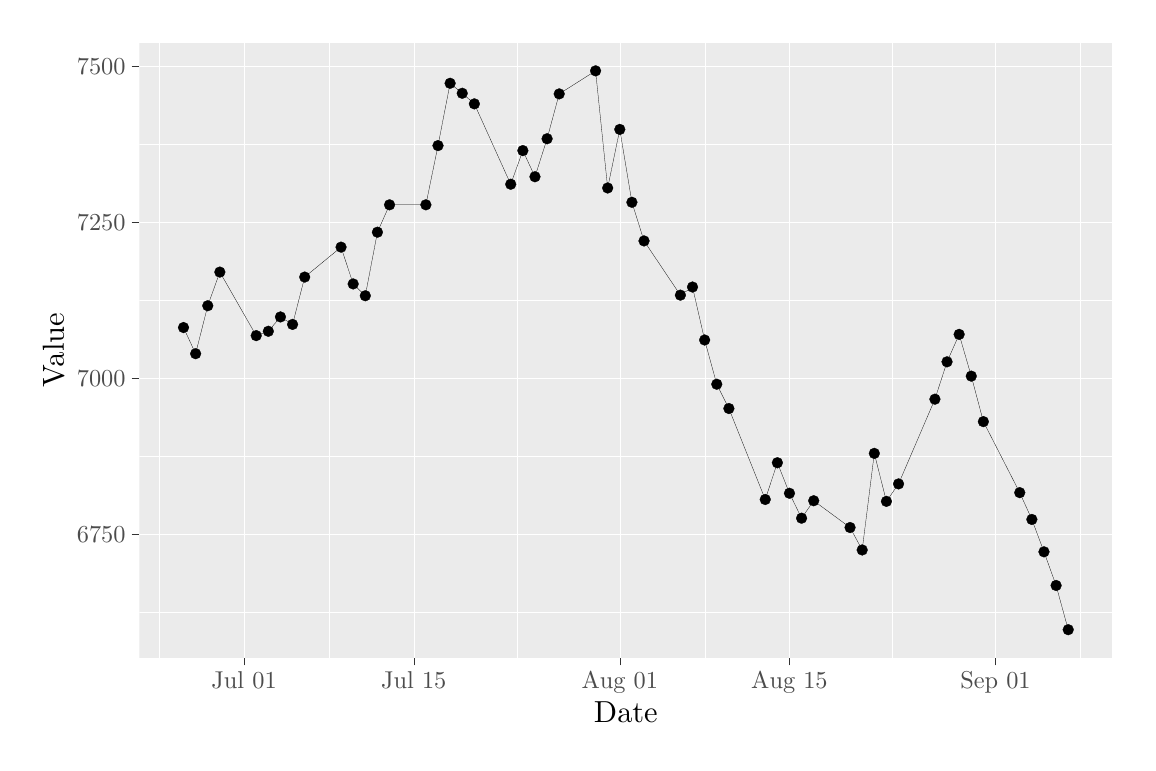
\begin{tikzpicture}[x=1pt,y=1pt]
\definecolor{fillColor}{RGB}{255,255,255}
\path[use as bounding box,fill=fillColor,fill opacity=0.00] (0,0) rectangle (397.48,258.37);
\begin{scope}
\path[clip] (  0.00,  0.00) rectangle (397.48,258.37);
\definecolor{drawColor}{RGB}{255,255,255}
\definecolor{fillColor}{RGB}{255,255,255}

\path[draw=drawColor,line width= 0.1pt,line join=round,line cap=round,fill=fillColor] (  0.00,  0.00) rectangle (397.48,258.37);
\end{scope}
\begin{scope}
\path[clip] ( 40.32, 30.73) rectangle (391.98,252.87);
\definecolor{fillColor}{gray}{0.92}

\path[fill=fillColor] ( 40.32, 30.73) rectangle (391.98,252.87);
\definecolor{drawColor}{RGB}{255,255,255}

\path[draw=drawColor,line width= 0.1pt,line join=round] ( 40.32, 47.35) --
	(391.98, 47.35);

\path[draw=drawColor,line width= 0.1pt,line join=round] ( 40.32,103.64) --
	(391.98,103.64);

\path[draw=drawColor,line width= 0.1pt,line join=round] ( 40.32,159.92) --
	(391.98,159.92);

\path[draw=drawColor,line width= 0.1pt,line join=round] ( 40.32,216.20) --
	(391.98,216.20);

\path[draw=drawColor,line width= 0.1pt,line join=round] ( 47.55, 30.73) --
	( 47.55,252.87);

\path[draw=drawColor,line width= 0.1pt,line join=round] (108.86, 30.73) --
	(108.86,252.87);

\path[draw=drawColor,line width= 0.1pt,line join=round] (176.74, 30.73) --
	(176.74,252.87);

\path[draw=drawColor,line width= 0.1pt,line join=round] (244.62, 30.73) --
	(244.62,252.87);

\path[draw=drawColor,line width= 0.1pt,line join=round] (312.50, 30.73) --
	(312.50,252.87);

\path[draw=drawColor,line width= 0.1pt,line join=round] (380.38, 30.73) --
	(380.38,252.87);

\path[draw=drawColor,line width= 0.1pt,line join=round] ( 40.32, 75.50) --
	(391.98, 75.50);

\path[draw=drawColor,line width= 0.1pt,line join=round] ( 40.32,131.78) --
	(391.98,131.78);

\path[draw=drawColor,line width= 0.1pt,line join=round] ( 40.32,188.06) --
	(391.98,188.06);

\path[draw=drawColor,line width= 0.1pt,line join=round] ( 40.32,244.34) --
	(391.98,244.34);

\path[draw=drawColor,line width= 0.1pt,line join=round] ( 78.20, 30.73) --
	( 78.20,252.87);

\path[draw=drawColor,line width= 0.1pt,line join=round] (139.51, 30.73) --
	(139.51,252.87);

\path[draw=drawColor,line width= 0.1pt,line join=round] (213.96, 30.73) --
	(213.96,252.87);

\path[draw=drawColor,line width= 0.1pt,line join=round] (275.27, 30.73) --
	(275.27,252.87);

\path[draw=drawColor,line width= 0.1pt,line join=round] (349.72, 30.73) --
	(349.72,252.87);
\definecolor{drawColor}{RGB}{0,0,0}

\path[draw=drawColor,line width= 0.1pt,line join=round] ( 56.31,150.01) --
	( 60.69,140.56) --
	( 65.07,157.89) --
	( 69.44,170.05) --
	( 82.58,147.09) --
	( 86.96,148.66) --
	( 91.34,153.84) --
	( 95.72,151.14) --
	(100.10,168.25) --
	(113.24,179.06) --
	(117.62,165.77) --
	(122.00,161.50) --
	(126.38,184.46) --
	(130.76,194.36) --
	(143.89,194.36) --
	(148.27,215.75) --
	(152.65,238.27) --
	(157.03,234.66) --
	(161.41,230.84) --
	(174.55,201.79) --
	(178.93,213.95) --
	(183.31,204.50) --
	(187.69,218.23) --
	(192.07,234.44) --
	(205.21,242.77) --
	(209.58,200.44) --
	(213.96,221.61) --
	(218.34,195.27) --
	(222.72,181.31) --
	(235.86,161.72) --
	(240.24,164.65) --
	(244.62,145.51) --
	(249.00,129.53) --
	(253.38,120.75) --
	(266.52, 87.88) --
	(270.90,101.16) --
	(275.27, 90.13) --
	(279.65, 81.12) --
	(284.03, 87.43) --
	(297.17, 77.75) --
	(301.55, 69.64) --
	(305.93,104.54) --
	(310.31, 87.20) --
	(314.69, 93.51) --
	(327.83,124.12) --
	(332.21,137.63) --
	(336.59,147.54) --
	(340.97,132.45) --
	(345.34,116.02) --
	(358.48, 90.35) --
	(362.86, 80.67) --
	(367.24, 68.97) --
	(371.62, 56.81) --
	(376.00, 40.83);
\definecolor{fillColor}{RGB}{0,0,0}

\path[draw=drawColor,line width= 0.1pt,line join=round,line cap=round,fill=fillColor] ( 56.31,150.01) circle (  1.96);

\path[draw=drawColor,line width= 0.1pt,line join=round,line cap=round,fill=fillColor] ( 60.69,140.56) circle (  1.96);

\path[draw=drawColor,line width= 0.1pt,line join=round,line cap=round,fill=fillColor] ( 65.07,157.89) circle (  1.96);

\path[draw=drawColor,line width= 0.1pt,line join=round,line cap=round,fill=fillColor] ( 69.44,170.05) circle (  1.96);

\path[draw=drawColor,line width= 0.1pt,line join=round,line cap=round,fill=fillColor] ( 82.58,147.09) circle (  1.96);

\path[draw=drawColor,line width= 0.1pt,line join=round,line cap=round,fill=fillColor] ( 86.96,148.66) circle (  1.96);

\path[draw=drawColor,line width= 0.1pt,line join=round,line cap=round,fill=fillColor] ( 91.34,153.84) circle (  1.96);

\path[draw=drawColor,line width= 0.1pt,line join=round,line cap=round,fill=fillColor] ( 95.72,151.14) circle (  1.96);

\path[draw=drawColor,line width= 0.1pt,line join=round,line cap=round,fill=fillColor] (100.10,168.25) circle (  1.96);

\path[draw=drawColor,line width= 0.1pt,line join=round,line cap=round,fill=fillColor] (113.24,179.06) circle (  1.96);

\path[draw=drawColor,line width= 0.1pt,line join=round,line cap=round,fill=fillColor] (117.62,165.77) circle (  1.96);

\path[draw=drawColor,line width= 0.1pt,line join=round,line cap=round,fill=fillColor] (122.00,161.50) circle (  1.96);

\path[draw=drawColor,line width= 0.1pt,line join=round,line cap=round,fill=fillColor] (126.38,184.46) circle (  1.96);

\path[draw=drawColor,line width= 0.1pt,line join=round,line cap=round,fill=fillColor] (130.76,194.36) circle (  1.96);

\path[draw=drawColor,line width= 0.1pt,line join=round,line cap=round,fill=fillColor] (143.89,194.36) circle (  1.96);

\path[draw=drawColor,line width= 0.1pt,line join=round,line cap=round,fill=fillColor] (148.27,215.75) circle (  1.96);

\path[draw=drawColor,line width= 0.1pt,line join=round,line cap=round,fill=fillColor] (152.65,238.27) circle (  1.96);

\path[draw=drawColor,line width= 0.1pt,line join=round,line cap=round,fill=fillColor] (157.03,234.66) circle (  1.96);

\path[draw=drawColor,line width= 0.1pt,line join=round,line cap=round,fill=fillColor] (161.41,230.84) circle (  1.96);

\path[draw=drawColor,line width= 0.1pt,line join=round,line cap=round,fill=fillColor] (174.55,201.79) circle (  1.96);

\path[draw=drawColor,line width= 0.1pt,line join=round,line cap=round,fill=fillColor] (178.93,213.95) circle (  1.96);

\path[draw=drawColor,line width= 0.1pt,line join=round,line cap=round,fill=fillColor] (183.31,204.50) circle (  1.96);

\path[draw=drawColor,line width= 0.1pt,line join=round,line cap=round,fill=fillColor] (187.69,218.23) circle (  1.96);

\path[draw=drawColor,line width= 0.1pt,line join=round,line cap=round,fill=fillColor] (192.07,234.44) circle (  1.96);

\path[draw=drawColor,line width= 0.1pt,line join=round,line cap=round,fill=fillColor] (205.21,242.77) circle (  1.96);

\path[draw=drawColor,line width= 0.1pt,line join=round,line cap=round,fill=fillColor] (209.58,200.44) circle (  1.96);

\path[draw=drawColor,line width= 0.1pt,line join=round,line cap=round,fill=fillColor] (213.96,221.61) circle (  1.96);

\path[draw=drawColor,line width= 0.1pt,line join=round,line cap=round,fill=fillColor] (218.34,195.27) circle (  1.96);

\path[draw=drawColor,line width= 0.1pt,line join=round,line cap=round,fill=fillColor] (222.72,181.31) circle (  1.96);

\path[draw=drawColor,line width= 0.1pt,line join=round,line cap=round,fill=fillColor] (235.86,161.72) circle (  1.96);

\path[draw=drawColor,line width= 0.1pt,line join=round,line cap=round,fill=fillColor] (240.24,164.65) circle (  1.96);

\path[draw=drawColor,line width= 0.1pt,line join=round,line cap=round,fill=fillColor] (244.62,145.51) circle (  1.96);

\path[draw=drawColor,line width= 0.1pt,line join=round,line cap=round,fill=fillColor] (249.00,129.53) circle (  1.96);

\path[draw=drawColor,line width= 0.1pt,line join=round,line cap=round,fill=fillColor] (253.38,120.75) circle (  1.96);

\path[draw=drawColor,line width= 0.1pt,line join=round,line cap=round,fill=fillColor] (266.52, 87.88) circle (  1.96);

\path[draw=drawColor,line width= 0.1pt,line join=round,line cap=round,fill=fillColor] (270.90,101.16) circle (  1.96);

\path[draw=drawColor,line width= 0.1pt,line join=round,line cap=round,fill=fillColor] (275.27, 90.13) circle (  1.96);

\path[draw=drawColor,line width= 0.1pt,line join=round,line cap=round,fill=fillColor] (279.65, 81.12) circle (  1.96);

\path[draw=drawColor,line width= 0.1pt,line join=round,line cap=round,fill=fillColor] (284.03, 87.43) circle (  1.96);

\path[draw=drawColor,line width= 0.1pt,line join=round,line cap=round,fill=fillColor] (297.17, 77.75) circle (  1.96);

\path[draw=drawColor,line width= 0.1pt,line join=round,line cap=round,fill=fillColor] (301.55, 69.64) circle (  1.96);

\path[draw=drawColor,line width= 0.1pt,line join=round,line cap=round,fill=fillColor] (305.93,104.54) circle (  1.96);

\path[draw=drawColor,line width= 0.1pt,line join=round,line cap=round,fill=fillColor] (310.31, 87.20) circle (  1.96);

\path[draw=drawColor,line width= 0.1pt,line join=round,line cap=round,fill=fillColor] (314.69, 93.51) circle (  1.96);

\path[draw=drawColor,line width= 0.1pt,line join=round,line cap=round,fill=fillColor] (327.83,124.12) circle (  1.96);

\path[draw=drawColor,line width= 0.1pt,line join=round,line cap=round,fill=fillColor] (332.21,137.63) circle (  1.96);

\path[draw=drawColor,line width= 0.1pt,line join=round,line cap=round,fill=fillColor] (336.59,147.54) circle (  1.96);

\path[draw=drawColor,line width= 0.1pt,line join=round,line cap=round,fill=fillColor] (340.97,132.45) circle (  1.96);

\path[draw=drawColor,line width= 0.1pt,line join=round,line cap=round,fill=fillColor] (345.34,116.02) circle (  1.96);

\path[draw=drawColor,line width= 0.1pt,line join=round,line cap=round,fill=fillColor] (358.48, 90.35) circle (  1.96);

\path[draw=drawColor,line width= 0.1pt,line join=round,line cap=round,fill=fillColor] (362.86, 80.67) circle (  1.96);

\path[draw=drawColor,line width= 0.1pt,line join=round,line cap=round,fill=fillColor] (367.24, 68.97) circle (  1.96);

\path[draw=drawColor,line width= 0.1pt,line join=round,line cap=round,fill=fillColor] (371.62, 56.81) circle (  1.96);

\path[draw=drawColor,line width= 0.1pt,line join=round,line cap=round,fill=fillColor] (376.00, 40.83) circle (  1.96);
\end{scope}
\begin{scope}
\path[clip] (  0.00,  0.00) rectangle (397.48,258.37);
\definecolor{drawColor}{gray}{0.30}

\node[text=drawColor,anchor=base east,inner sep=0pt, outer sep=0pt, scale=  0.88] at ( 35.37, 72.46) {6750};

\node[text=drawColor,anchor=base east,inner sep=0pt, outer sep=0pt, scale=  0.88] at ( 35.37,128.75) {7000};

\node[text=drawColor,anchor=base east,inner sep=0pt, outer sep=0pt, scale=  0.88] at ( 35.37,185.03) {7250};

\node[text=drawColor,anchor=base east,inner sep=0pt, outer sep=0pt, scale=  0.88] at ( 35.37,241.31) {7500};
\end{scope}
\begin{scope}
\path[clip] (  0.00,  0.00) rectangle (397.48,258.37);
\definecolor{drawColor}{gray}{0.20}

\path[draw=drawColor,line width= 0.1pt,line join=round] ( 37.57, 75.50) --
	( 40.32, 75.50);

\path[draw=drawColor,line width= 0.1pt,line join=round] ( 37.57,131.78) --
	( 40.32,131.78);

\path[draw=drawColor,line width= 0.1pt,line join=round] ( 37.57,188.06) --
	( 40.32,188.06);

\path[draw=drawColor,line width= 0.1pt,line join=round] ( 37.57,244.34) --
	( 40.32,244.34);
\end{scope}
\begin{scope}
\path[clip] (  0.00,  0.00) rectangle (397.48,258.37);
\definecolor{drawColor}{gray}{0.20}

\path[draw=drawColor,line width= 0.1pt,line join=round] ( 78.20, 27.98) --
	( 78.20, 30.73);

\path[draw=drawColor,line width= 0.1pt,line join=round] (139.51, 27.98) --
	(139.51, 30.73);

\path[draw=drawColor,line width= 0.1pt,line join=round] (213.96, 27.98) --
	(213.96, 30.73);

\path[draw=drawColor,line width= 0.1pt,line join=round] (275.27, 27.98) --
	(275.27, 30.73);

\path[draw=drawColor,line width= 0.1pt,line join=round] (349.72, 27.98) --
	(349.72, 30.73);
\end{scope}
\begin{scope}
\path[clip] (  0.00,  0.00) rectangle (397.48,258.37);
\definecolor{drawColor}{gray}{0.30}

\node[text=drawColor,anchor=base,inner sep=0pt, outer sep=0pt, scale=  0.88] at ( 78.20, 19.72) {Jul 01};

\node[text=drawColor,anchor=base,inner sep=0pt, outer sep=0pt, scale=  0.88] at (139.51, 19.72) {Jul 15};

\node[text=drawColor,anchor=base,inner sep=0pt, outer sep=0pt, scale=  0.88] at (213.96, 19.72) {Aug 01};

\node[text=drawColor,anchor=base,inner sep=0pt, outer sep=0pt, scale=  0.88] at (275.27, 19.72) {Aug 15};

\node[text=drawColor,anchor=base,inner sep=0pt, outer sep=0pt, scale=  0.88] at (349.72, 19.72) {Sep 01};
\end{scope}
\begin{scope}
\path[clip] (  0.00,  0.00) rectangle (397.48,258.37);
\definecolor{drawColor}{RGB}{0,0,0}

\node[text=drawColor,anchor=base,inner sep=0pt, outer sep=0pt, scale=  1.10] at (216.15,  7.44) {Date};
\end{scope}
\begin{scope}
\path[clip] (  0.00,  0.00) rectangle (397.48,258.37);
\definecolor{drawColor}{RGB}{0,0,0}

\node[text=drawColor,rotate= 90.00,anchor=base,inner sep=0pt, outer sep=0pt, scale=  1.10] at ( 13.08,141.80) {Value};
\end{scope}
\end{tikzpicture}

    \caption{\indicesCaption{\toyota}}
    \label{fig:analysis-indices-toyota}
\end{figure}   

\subsection{\vw}
\label{ss:analysis-datasets-vw}

%             From         To Days  Tweets
% DG#0  2018-02-28 2018-04-08   40 3001535
% DG#4  2018-06-26 2018-07-03    8  765042
% DG#5  2018-07-19 2018-08-01   14  955986
% DG#6  2018-08-20 2018-09-05   17 1496787
% Total 2018-02-28 2018-09-05   79 6219350

For the \vw\ \num{6219350} english tweets have been captured in total between \printdate{2018-02-28} and \printdate{2018-09-05}.
But as stated earlier in \cref{ss:casestudy-gatherdata-tweets} this was not a continuous time frame.
The various collected time frames, number of consecutive days in each frame and collected tweets in that frame are depicted in \cref{tab:anaylsis-datasets-vw}.

\begin{table}[hbt]
    \centering
    \begin{tabular}{!>{\bfseries}l ^l ^l ^r ^r}
      \hline
      \rowstyle{\bfseries}
                & From & To & \# Days & \# Tweets \\ \hline
        Group 1 & \printdate{2018-02-28} & \printdate{2018-04-08} &   \num{40} & \num{3001535} \\
        Group 2 & \printdate{2018-06-26} & \printdate{2018-07-03} &   \num{08} & \num{765042} \\
        Group 3 & \printdate{2018-07-19} & \printdate{2018-08-01} &   \num{14} & \num{955986} \\
        Group 4 & \printdate{2018-08-20} & \printdate{2018-09-05} &   \num{17} & \num{1496787} \\ \hline
        Total   & \printdate{2018-02-28} & \printdate{2018-09-05} &   \num{96} & \num{6219350} \\ \hline
    \end{tabular}
  
    \caption{\tweetsCaption{\vw}}
    \label{tab:anaylsis-datasets-vw}
\end{table}

Therefore, share prices have been downloaded for the given time frame which is depicted in \cref{fig:analysis-indices-vw}.

\begin{figure}[hbt]
    \centering
    % Created by tikzDevice version 0.12 on 2019-02-27 11:50:37
% !TEX encoding = UTF-8 Unicode
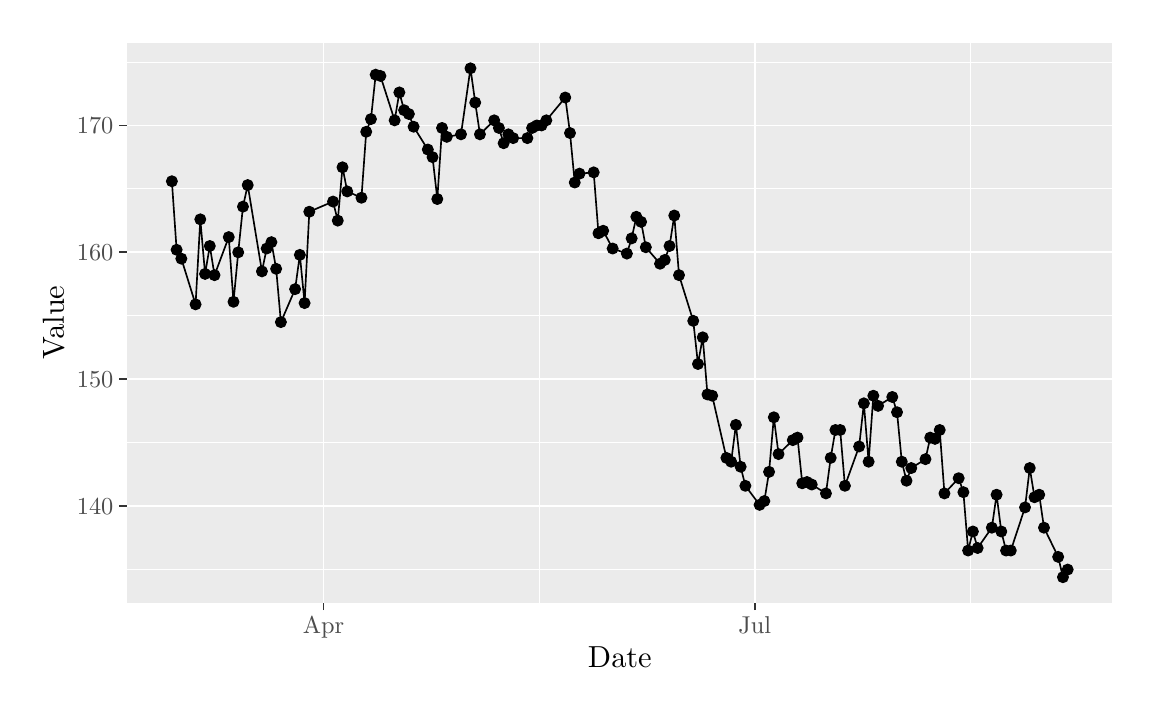
\begin{tikzpicture}[x=1pt,y=1pt]
\definecolor{fillColor}{RGB}{255,255,255}
\path[use as bounding box,fill=fillColor,fill opacity=0.00] (0,0) rectangle (397.48,238.49);
\begin{scope}
\path[clip] (  0.00,  0.00) rectangle (397.48,238.49);
\definecolor{drawColor}{RGB}{255,255,255}
\definecolor{fillColor}{RGB}{255,255,255}

\path[draw=drawColor,line width= 0.6pt,line join=round,line cap=round,fill=fillColor] (  0.00,  0.00) rectangle (397.48,238.49);
\end{scope}
\begin{scope}
\path[clip] ( 35.92, 30.73) rectangle (391.98,232.99);
\definecolor{fillColor}{gray}{0.92}

\path[fill=fillColor] ( 35.92, 30.73) rectangle (391.98,232.99);
\definecolor{drawColor}{RGB}{255,255,255}

\path[draw=drawColor,line width= 0.3pt,line join=round] ( 35.92, 42.67) --
	(391.98, 42.67);

\path[draw=drawColor,line width= 0.3pt,line join=round] ( 35.92, 88.53) --
	(391.98, 88.53);

\path[draw=drawColor,line width= 0.3pt,line join=round] ( 35.92,134.38) --
	(391.98,134.38);

\path[draw=drawColor,line width= 0.3pt,line join=round] ( 35.92,180.24) --
	(391.98,180.24);

\path[draw=drawColor,line width= 0.3pt,line join=round] ( 35.92,226.09) --
	(391.98,226.09);

\path[draw=drawColor,line width= 0.3pt,line join=round] (184.84, 30.73) --
	(184.84,232.99);

\path[draw=drawColor,line width= 0.3pt,line join=round] (340.69, 30.73) --
	(340.69,232.99);

\path[draw=drawColor,line width= 0.6pt,line join=round] ( 35.92, 65.60) --
	(391.98, 65.60);

\path[draw=drawColor,line width= 0.6pt,line join=round] ( 35.92,111.45) --
	(391.98,111.45);

\path[draw=drawColor,line width= 0.6pt,line join=round] ( 35.92,157.31) --
	(391.98,157.31);

\path[draw=drawColor,line width= 0.6pt,line join=round] ( 35.92,203.16) --
	(391.98,203.16);

\path[draw=drawColor,line width= 0.6pt,line join=round] (106.91, 30.73) --
	(106.91,232.99);

\path[draw=drawColor,line width= 0.6pt,line join=round] (262.76, 30.73) --
	(262.76,232.99);
\definecolor{drawColor}{RGB}{0,0,0}

\path[draw=drawColor,line width= 0.6pt,line join=round] ( 52.11,182.99) --
	( 53.82,158.23) --
	( 55.53,155.02) --
	( 60.67,138.51) --
	( 62.38,169.23) --
	( 64.10,149.51) --
	( 65.81,159.60) --
	( 67.52,149.06) --
	( 72.66,162.81) --
	( 74.37,139.43) --
	( 76.08,157.31) --
	( 77.80,173.82) --
	( 79.51,181.61) --
	( 84.65,150.43) --
	( 86.36,158.68) --
	( 88.07,160.98) --
	( 89.79,151.35) --
	( 91.50,132.09) --
	( 96.64,144.01) --
	( 98.35,156.39) --
	(100.06,138.97) --
	(101.77,171.98) --
	(110.34,175.65) --
	(112.05,168.77) --
	(113.76,188.03) --
	(115.48,179.32) --
	(120.61,177.03) --
	(122.33,200.87) --
	(124.04,205.46) --
	(125.75,221.50) --
	(127.46,221.05) --
	(132.60,205.00) --
	(134.31,215.09) --
	(136.03,208.67) --
	(137.74,207.29) --
	(139.45,202.70) --
	(144.59,194.45) --
	(146.30,191.70) --
	(148.02,176.57) --
	(149.73,202.25) --
	(151.44,199.04) --
	(156.58,199.95) --
	(160.00,223.80) --
	(161.72,211.42) --
	(163.43,199.95) --
	(168.57,205.00) --
	(170.28,202.25) --
	(171.99,196.74) --
	(173.71,199.95) --
	(175.42,198.58) --
	(180.56,198.58) --
	(182.27,202.25) --
	(183.98,203.16) --
	(185.69,203.16) --
	(187.41,205.00) --
	(194.26,213.25) --
	(195.97,200.41) --
	(197.68,182.53) --
	(199.40,185.74) --
	(204.53,186.20) --
	(206.25,164.19) --
	(207.96,165.10) --
	(211.38,158.68) --
	(216.52,156.85) --
	(218.24,162.35) --
	(219.95,170.15) --
	(221.66,168.31) --
	(223.37,159.14) --
	(228.51,153.18) --
	(230.22,154.56) --
	(231.94,159.60) --
	(233.65,170.61) --
	(235.36,149.06) --
	(240.50,132.55) --
	(242.21,116.96) --
	(243.93,126.59) --
	(245.64,105.95) --
	(247.35,105.49) --
	(252.49, 83.03) --
	(254.20, 81.65) --
	(255.91, 94.95) --
	(257.63, 79.82) --
	(259.34, 72.94) --
	(264.48, 66.06) --
	(266.19, 67.43) --
	(267.90, 77.98) --
	(269.62, 97.70) --
	(271.33, 84.40) --
	(276.47, 89.44) --
	(278.18, 90.36) --
	(279.89, 73.85) --
	(281.60, 74.31) --
	(283.32, 73.40) --
	(288.45, 70.19) --
	(290.17, 83.03) --
	(291.88, 93.11) --
	(293.59, 93.11) --
	(295.31, 72.94) --
	(300.44, 87.15) --
	(302.16,102.74) --
	(303.87, 81.65) --
	(305.58,105.49) --
	(307.29,101.83) --
	(312.43,105.04) --
	(314.14, 99.53) --
	(315.86, 81.65) --
	(317.57, 74.77) --
	(319.28, 79.36) --
	(324.42, 82.57) --
	(326.13, 90.36) --
	(327.85, 89.90) --
	(329.56, 93.11) --
	(331.27, 70.19) --
	(336.41, 75.69) --
	(338.12, 70.64) --
	(339.83, 49.55) --
	(341.55, 56.43) --
	(343.26, 50.47) --
	(348.40, 57.81) --
	(350.11, 69.73) --
	(351.82, 56.43) --
	(353.54, 49.55) --
	(355.25, 49.55) --
	(360.39, 65.14) --
	(362.10, 79.36) --
	(363.81, 68.81) --
	(365.52, 69.73) --
	(367.24, 57.81) --
	(372.37, 47.26) --
	(374.09, 39.92) --
	(375.80, 42.67);
\definecolor{fillColor}{RGB}{0,0,0}

\path[draw=drawColor,line width= 0.4pt,line join=round,line cap=round,fill=fillColor] ( 52.11,182.99) circle (  1.96);

\path[draw=drawColor,line width= 0.4pt,line join=round,line cap=round,fill=fillColor] ( 53.82,158.23) circle (  1.96);

\path[draw=drawColor,line width= 0.4pt,line join=round,line cap=round,fill=fillColor] ( 55.53,155.02) circle (  1.96);

\path[draw=drawColor,line width= 0.4pt,line join=round,line cap=round,fill=fillColor] ( 60.67,138.51) circle (  1.96);

\path[draw=drawColor,line width= 0.4pt,line join=round,line cap=round,fill=fillColor] ( 62.38,169.23) circle (  1.96);

\path[draw=drawColor,line width= 0.4pt,line join=round,line cap=round,fill=fillColor] ( 64.10,149.51) circle (  1.96);

\path[draw=drawColor,line width= 0.4pt,line join=round,line cap=round,fill=fillColor] ( 65.81,159.60) circle (  1.96);

\path[draw=drawColor,line width= 0.4pt,line join=round,line cap=round,fill=fillColor] ( 67.52,149.06) circle (  1.96);

\path[draw=drawColor,line width= 0.4pt,line join=round,line cap=round,fill=fillColor] ( 72.66,162.81) circle (  1.96);

\path[draw=drawColor,line width= 0.4pt,line join=round,line cap=round,fill=fillColor] ( 74.37,139.43) circle (  1.96);

\path[draw=drawColor,line width= 0.4pt,line join=round,line cap=round,fill=fillColor] ( 76.08,157.31) circle (  1.96);

\path[draw=drawColor,line width= 0.4pt,line join=round,line cap=round,fill=fillColor] ( 77.80,173.82) circle (  1.96);

\path[draw=drawColor,line width= 0.4pt,line join=round,line cap=round,fill=fillColor] ( 79.51,181.61) circle (  1.96);

\path[draw=drawColor,line width= 0.4pt,line join=round,line cap=round,fill=fillColor] ( 84.65,150.43) circle (  1.96);

\path[draw=drawColor,line width= 0.4pt,line join=round,line cap=round,fill=fillColor] ( 86.36,158.68) circle (  1.96);

\path[draw=drawColor,line width= 0.4pt,line join=round,line cap=round,fill=fillColor] ( 88.07,160.98) circle (  1.96);

\path[draw=drawColor,line width= 0.4pt,line join=round,line cap=round,fill=fillColor] ( 89.79,151.35) circle (  1.96);

\path[draw=drawColor,line width= 0.4pt,line join=round,line cap=round,fill=fillColor] ( 91.50,132.09) circle (  1.96);

\path[draw=drawColor,line width= 0.4pt,line join=round,line cap=round,fill=fillColor] ( 96.64,144.01) circle (  1.96);

\path[draw=drawColor,line width= 0.4pt,line join=round,line cap=round,fill=fillColor] ( 98.35,156.39) circle (  1.96);

\path[draw=drawColor,line width= 0.4pt,line join=round,line cap=round,fill=fillColor] (100.06,138.97) circle (  1.96);

\path[draw=drawColor,line width= 0.4pt,line join=round,line cap=round,fill=fillColor] (101.77,171.98) circle (  1.96);

\path[draw=drawColor,line width= 0.4pt,line join=round,line cap=round,fill=fillColor] (110.34,175.65) circle (  1.96);

\path[draw=drawColor,line width= 0.4pt,line join=round,line cap=round,fill=fillColor] (112.05,168.77) circle (  1.96);

\path[draw=drawColor,line width= 0.4pt,line join=round,line cap=round,fill=fillColor] (113.76,188.03) circle (  1.96);

\path[draw=drawColor,line width= 0.4pt,line join=round,line cap=round,fill=fillColor] (115.48,179.32) circle (  1.96);

\path[draw=drawColor,line width= 0.4pt,line join=round,line cap=round,fill=fillColor] (120.61,177.03) circle (  1.96);

\path[draw=drawColor,line width= 0.4pt,line join=round,line cap=round,fill=fillColor] (122.33,200.87) circle (  1.96);

\path[draw=drawColor,line width= 0.4pt,line join=round,line cap=round,fill=fillColor] (124.04,205.46) circle (  1.96);

\path[draw=drawColor,line width= 0.4pt,line join=round,line cap=round,fill=fillColor] (125.75,221.50) circle (  1.96);

\path[draw=drawColor,line width= 0.4pt,line join=round,line cap=round,fill=fillColor] (127.46,221.05) circle (  1.96);

\path[draw=drawColor,line width= 0.4pt,line join=round,line cap=round,fill=fillColor] (132.60,205.00) circle (  1.96);

\path[draw=drawColor,line width= 0.4pt,line join=round,line cap=round,fill=fillColor] (134.31,215.09) circle (  1.96);

\path[draw=drawColor,line width= 0.4pt,line join=round,line cap=round,fill=fillColor] (136.03,208.67) circle (  1.96);

\path[draw=drawColor,line width= 0.4pt,line join=round,line cap=round,fill=fillColor] (137.74,207.29) circle (  1.96);

\path[draw=drawColor,line width= 0.4pt,line join=round,line cap=round,fill=fillColor] (139.45,202.70) circle (  1.96);

\path[draw=drawColor,line width= 0.4pt,line join=round,line cap=round,fill=fillColor] (144.59,194.45) circle (  1.96);

\path[draw=drawColor,line width= 0.4pt,line join=round,line cap=round,fill=fillColor] (146.30,191.70) circle (  1.96);

\path[draw=drawColor,line width= 0.4pt,line join=round,line cap=round,fill=fillColor] (148.02,176.57) circle (  1.96);

\path[draw=drawColor,line width= 0.4pt,line join=round,line cap=round,fill=fillColor] (149.73,202.25) circle (  1.96);

\path[draw=drawColor,line width= 0.4pt,line join=round,line cap=round,fill=fillColor] (151.44,199.04) circle (  1.96);

\path[draw=drawColor,line width= 0.4pt,line join=round,line cap=round,fill=fillColor] (156.58,199.95) circle (  1.96);

\path[draw=drawColor,line width= 0.4pt,line join=round,line cap=round,fill=fillColor] (160.00,223.80) circle (  1.96);

\path[draw=drawColor,line width= 0.4pt,line join=round,line cap=round,fill=fillColor] (161.72,211.42) circle (  1.96);

\path[draw=drawColor,line width= 0.4pt,line join=round,line cap=round,fill=fillColor] (163.43,199.95) circle (  1.96);

\path[draw=drawColor,line width= 0.4pt,line join=round,line cap=round,fill=fillColor] (168.57,205.00) circle (  1.96);

\path[draw=drawColor,line width= 0.4pt,line join=round,line cap=round,fill=fillColor] (170.28,202.25) circle (  1.96);

\path[draw=drawColor,line width= 0.4pt,line join=round,line cap=round,fill=fillColor] (171.99,196.74) circle (  1.96);

\path[draw=drawColor,line width= 0.4pt,line join=round,line cap=round,fill=fillColor] (173.71,199.95) circle (  1.96);

\path[draw=drawColor,line width= 0.4pt,line join=round,line cap=round,fill=fillColor] (175.42,198.58) circle (  1.96);

\path[draw=drawColor,line width= 0.4pt,line join=round,line cap=round,fill=fillColor] (180.56,198.58) circle (  1.96);

\path[draw=drawColor,line width= 0.4pt,line join=round,line cap=round,fill=fillColor] (182.27,202.25) circle (  1.96);

\path[draw=drawColor,line width= 0.4pt,line join=round,line cap=round,fill=fillColor] (183.98,203.16) circle (  1.96);

\path[draw=drawColor,line width= 0.4pt,line join=round,line cap=round,fill=fillColor] (185.69,203.16) circle (  1.96);

\path[draw=drawColor,line width= 0.4pt,line join=round,line cap=round,fill=fillColor] (187.41,205.00) circle (  1.96);

\path[draw=drawColor,line width= 0.4pt,line join=round,line cap=round,fill=fillColor] (194.26,213.25) circle (  1.96);

\path[draw=drawColor,line width= 0.4pt,line join=round,line cap=round,fill=fillColor] (195.97,200.41) circle (  1.96);

\path[draw=drawColor,line width= 0.4pt,line join=round,line cap=round,fill=fillColor] (197.68,182.53) circle (  1.96);

\path[draw=drawColor,line width= 0.4pt,line join=round,line cap=round,fill=fillColor] (199.40,185.74) circle (  1.96);

\path[draw=drawColor,line width= 0.4pt,line join=round,line cap=round,fill=fillColor] (204.53,186.20) circle (  1.96);

\path[draw=drawColor,line width= 0.4pt,line join=round,line cap=round,fill=fillColor] (206.25,164.19) circle (  1.96);

\path[draw=drawColor,line width= 0.4pt,line join=round,line cap=round,fill=fillColor] (207.96,165.10) circle (  1.96);

\path[draw=drawColor,line width= 0.4pt,line join=round,line cap=round,fill=fillColor] (211.38,158.68) circle (  1.96);

\path[draw=drawColor,line width= 0.4pt,line join=round,line cap=round,fill=fillColor] (216.52,156.85) circle (  1.96);

\path[draw=drawColor,line width= 0.4pt,line join=round,line cap=round,fill=fillColor] (218.24,162.35) circle (  1.96);

\path[draw=drawColor,line width= 0.4pt,line join=round,line cap=round,fill=fillColor] (219.95,170.15) circle (  1.96);

\path[draw=drawColor,line width= 0.4pt,line join=round,line cap=round,fill=fillColor] (221.66,168.31) circle (  1.96);

\path[draw=drawColor,line width= 0.4pt,line join=round,line cap=round,fill=fillColor] (223.37,159.14) circle (  1.96);

\path[draw=drawColor,line width= 0.4pt,line join=round,line cap=round,fill=fillColor] (228.51,153.18) circle (  1.96);

\path[draw=drawColor,line width= 0.4pt,line join=round,line cap=round,fill=fillColor] (230.22,154.56) circle (  1.96);

\path[draw=drawColor,line width= 0.4pt,line join=round,line cap=round,fill=fillColor] (231.94,159.60) circle (  1.96);

\path[draw=drawColor,line width= 0.4pt,line join=round,line cap=round,fill=fillColor] (233.65,170.61) circle (  1.96);

\path[draw=drawColor,line width= 0.4pt,line join=round,line cap=round,fill=fillColor] (235.36,149.06) circle (  1.96);

\path[draw=drawColor,line width= 0.4pt,line join=round,line cap=round,fill=fillColor] (240.50,132.55) circle (  1.96);

\path[draw=drawColor,line width= 0.4pt,line join=round,line cap=round,fill=fillColor] (242.21,116.96) circle (  1.96);

\path[draw=drawColor,line width= 0.4pt,line join=round,line cap=round,fill=fillColor] (243.93,126.59) circle (  1.96);

\path[draw=drawColor,line width= 0.4pt,line join=round,line cap=round,fill=fillColor] (245.64,105.95) circle (  1.96);

\path[draw=drawColor,line width= 0.4pt,line join=round,line cap=round,fill=fillColor] (247.35,105.49) circle (  1.96);

\path[draw=drawColor,line width= 0.4pt,line join=round,line cap=round,fill=fillColor] (252.49, 83.03) circle (  1.96);

\path[draw=drawColor,line width= 0.4pt,line join=round,line cap=round,fill=fillColor] (254.20, 81.65) circle (  1.96);

\path[draw=drawColor,line width= 0.4pt,line join=round,line cap=round,fill=fillColor] (255.91, 94.95) circle (  1.96);

\path[draw=drawColor,line width= 0.4pt,line join=round,line cap=round,fill=fillColor] (257.63, 79.82) circle (  1.96);

\path[draw=drawColor,line width= 0.4pt,line join=round,line cap=round,fill=fillColor] (259.34, 72.94) circle (  1.96);

\path[draw=drawColor,line width= 0.4pt,line join=round,line cap=round,fill=fillColor] (264.48, 66.06) circle (  1.96);

\path[draw=drawColor,line width= 0.4pt,line join=round,line cap=round,fill=fillColor] (266.19, 67.43) circle (  1.96);

\path[draw=drawColor,line width= 0.4pt,line join=round,line cap=round,fill=fillColor] (267.90, 77.98) circle (  1.96);

\path[draw=drawColor,line width= 0.4pt,line join=round,line cap=round,fill=fillColor] (269.62, 97.70) circle (  1.96);

\path[draw=drawColor,line width= 0.4pt,line join=round,line cap=round,fill=fillColor] (271.33, 84.40) circle (  1.96);

\path[draw=drawColor,line width= 0.4pt,line join=round,line cap=round,fill=fillColor] (276.47, 89.44) circle (  1.96);

\path[draw=drawColor,line width= 0.4pt,line join=round,line cap=round,fill=fillColor] (278.18, 90.36) circle (  1.96);

\path[draw=drawColor,line width= 0.4pt,line join=round,line cap=round,fill=fillColor] (279.89, 73.85) circle (  1.96);

\path[draw=drawColor,line width= 0.4pt,line join=round,line cap=round,fill=fillColor] (281.60, 74.31) circle (  1.96);

\path[draw=drawColor,line width= 0.4pt,line join=round,line cap=round,fill=fillColor] (283.32, 73.40) circle (  1.96);

\path[draw=drawColor,line width= 0.4pt,line join=round,line cap=round,fill=fillColor] (288.45, 70.19) circle (  1.96);

\path[draw=drawColor,line width= 0.4pt,line join=round,line cap=round,fill=fillColor] (290.17, 83.03) circle (  1.96);

\path[draw=drawColor,line width= 0.4pt,line join=round,line cap=round,fill=fillColor] (291.88, 93.11) circle (  1.96);

\path[draw=drawColor,line width= 0.4pt,line join=round,line cap=round,fill=fillColor] (293.59, 93.11) circle (  1.96);

\path[draw=drawColor,line width= 0.4pt,line join=round,line cap=round,fill=fillColor] (295.31, 72.94) circle (  1.96);

\path[draw=drawColor,line width= 0.4pt,line join=round,line cap=round,fill=fillColor] (300.44, 87.15) circle (  1.96);

\path[draw=drawColor,line width= 0.4pt,line join=round,line cap=round,fill=fillColor] (302.16,102.74) circle (  1.96);

\path[draw=drawColor,line width= 0.4pt,line join=round,line cap=round,fill=fillColor] (303.87, 81.65) circle (  1.96);

\path[draw=drawColor,line width= 0.4pt,line join=round,line cap=round,fill=fillColor] (305.58,105.49) circle (  1.96);

\path[draw=drawColor,line width= 0.4pt,line join=round,line cap=round,fill=fillColor] (307.29,101.83) circle (  1.96);

\path[draw=drawColor,line width= 0.4pt,line join=round,line cap=round,fill=fillColor] (312.43,105.04) circle (  1.96);

\path[draw=drawColor,line width= 0.4pt,line join=round,line cap=round,fill=fillColor] (314.14, 99.53) circle (  1.96);

\path[draw=drawColor,line width= 0.4pt,line join=round,line cap=round,fill=fillColor] (315.86, 81.65) circle (  1.96);

\path[draw=drawColor,line width= 0.4pt,line join=round,line cap=round,fill=fillColor] (317.57, 74.77) circle (  1.96);

\path[draw=drawColor,line width= 0.4pt,line join=round,line cap=round,fill=fillColor] (319.28, 79.36) circle (  1.96);

\path[draw=drawColor,line width= 0.4pt,line join=round,line cap=round,fill=fillColor] (324.42, 82.57) circle (  1.96);

\path[draw=drawColor,line width= 0.4pt,line join=round,line cap=round,fill=fillColor] (326.13, 90.36) circle (  1.96);

\path[draw=drawColor,line width= 0.4pt,line join=round,line cap=round,fill=fillColor] (327.85, 89.90) circle (  1.96);

\path[draw=drawColor,line width= 0.4pt,line join=round,line cap=round,fill=fillColor] (329.56, 93.11) circle (  1.96);

\path[draw=drawColor,line width= 0.4pt,line join=round,line cap=round,fill=fillColor] (331.27, 70.19) circle (  1.96);

\path[draw=drawColor,line width= 0.4pt,line join=round,line cap=round,fill=fillColor] (336.41, 75.69) circle (  1.96);

\path[draw=drawColor,line width= 0.4pt,line join=round,line cap=round,fill=fillColor] (338.12, 70.64) circle (  1.96);

\path[draw=drawColor,line width= 0.4pt,line join=round,line cap=round,fill=fillColor] (339.83, 49.55) circle (  1.96);

\path[draw=drawColor,line width= 0.4pt,line join=round,line cap=round,fill=fillColor] (341.55, 56.43) circle (  1.96);

\path[draw=drawColor,line width= 0.4pt,line join=round,line cap=round,fill=fillColor] (343.26, 50.47) circle (  1.96);

\path[draw=drawColor,line width= 0.4pt,line join=round,line cap=round,fill=fillColor] (348.40, 57.81) circle (  1.96);

\path[draw=drawColor,line width= 0.4pt,line join=round,line cap=round,fill=fillColor] (350.11, 69.73) circle (  1.96);

\path[draw=drawColor,line width= 0.4pt,line join=round,line cap=round,fill=fillColor] (351.82, 56.43) circle (  1.96);

\path[draw=drawColor,line width= 0.4pt,line join=round,line cap=round,fill=fillColor] (353.54, 49.55) circle (  1.96);

\path[draw=drawColor,line width= 0.4pt,line join=round,line cap=round,fill=fillColor] (355.25, 49.55) circle (  1.96);

\path[draw=drawColor,line width= 0.4pt,line join=round,line cap=round,fill=fillColor] (360.39, 65.14) circle (  1.96);

\path[draw=drawColor,line width= 0.4pt,line join=round,line cap=round,fill=fillColor] (362.10, 79.36) circle (  1.96);

\path[draw=drawColor,line width= 0.4pt,line join=round,line cap=round,fill=fillColor] (363.81, 68.81) circle (  1.96);

\path[draw=drawColor,line width= 0.4pt,line join=round,line cap=round,fill=fillColor] (365.52, 69.73) circle (  1.96);

\path[draw=drawColor,line width= 0.4pt,line join=round,line cap=round,fill=fillColor] (367.24, 57.81) circle (  1.96);

\path[draw=drawColor,line width= 0.4pt,line join=round,line cap=round,fill=fillColor] (372.37, 47.26) circle (  1.96);

\path[draw=drawColor,line width= 0.4pt,line join=round,line cap=round,fill=fillColor] (374.09, 39.92) circle (  1.96);

\path[draw=drawColor,line width= 0.4pt,line join=round,line cap=round,fill=fillColor] (375.80, 42.67) circle (  1.96);
\end{scope}
\begin{scope}
\path[clip] (  0.00,  0.00) rectangle (397.48,238.49);
\definecolor{drawColor}{gray}{0.30}

\node[text=drawColor,anchor=base east,inner sep=0pt, outer sep=0pt, scale=  0.88] at ( 30.97, 62.57) {140};

\node[text=drawColor,anchor=base east,inner sep=0pt, outer sep=0pt, scale=  0.88] at ( 30.97,108.42) {150};

\node[text=drawColor,anchor=base east,inner sep=0pt, outer sep=0pt, scale=  0.88] at ( 30.97,154.28) {160};

\node[text=drawColor,anchor=base east,inner sep=0pt, outer sep=0pt, scale=  0.88] at ( 30.97,200.13) {170};
\end{scope}
\begin{scope}
\path[clip] (  0.00,  0.00) rectangle (397.48,238.49);
\definecolor{drawColor}{gray}{0.20}

\path[draw=drawColor,line width= 0.6pt,line join=round] ( 33.17, 65.60) --
	( 35.92, 65.60);

\path[draw=drawColor,line width= 0.6pt,line join=round] ( 33.17,111.45) --
	( 35.92,111.45);

\path[draw=drawColor,line width= 0.6pt,line join=round] ( 33.17,157.31) --
	( 35.92,157.31);

\path[draw=drawColor,line width= 0.6pt,line join=round] ( 33.17,203.16) --
	( 35.92,203.16);
\end{scope}
\begin{scope}
\path[clip] (  0.00,  0.00) rectangle (397.48,238.49);
\definecolor{drawColor}{gray}{0.20}

\path[draw=drawColor,line width= 0.6pt,line join=round] (106.91, 27.98) --
	(106.91, 30.73);

\path[draw=drawColor,line width= 0.6pt,line join=round] (262.76, 27.98) --
	(262.76, 30.73);
\end{scope}
\begin{scope}
\path[clip] (  0.00,  0.00) rectangle (397.48,238.49);
\definecolor{drawColor}{gray}{0.30}

\node[text=drawColor,anchor=base,inner sep=0pt, outer sep=0pt, scale=  0.88] at (106.91, 19.72) {Apr};

\node[text=drawColor,anchor=base,inner sep=0pt, outer sep=0pt, scale=  0.88] at (262.76, 19.72) {Jul};
\end{scope}
\begin{scope}
\path[clip] (  0.00,  0.00) rectangle (397.48,238.49);
\definecolor{drawColor}{RGB}{0,0,0}

\node[text=drawColor,anchor=base,inner sep=0pt, outer sep=0pt, scale=  1.10] at (213.95,  7.44) {Date};
\end{scope}
\begin{scope}
\path[clip] (  0.00,  0.00) rectangle (397.48,238.49);
\definecolor{drawColor}{RGB}{0,0,0}

\node[text=drawColor,rotate= 90.00,anchor=base,inner sep=0pt, outer sep=0pt, scale=  1.10] at ( 13.08,131.86) {Value};
\end{scope}
\end{tikzpicture}

    \caption{\indicesCaption{\vw}}
    \label{fig:analysis-indices-vw}
\end{figure}   

\section{Hyper-parameters}
\label{s:analysis-pipelines}
% best estimator pipeline

This section presents the results of the model selector GridSearchCV as described in \cref{s:casestudy-sentiment}.
GridSearchCV has been trained and tested using the Twitter corpus of \ac{NLTK} (\emph{nltk.corpus.twitter\_samples}) which contains each \num{5000} positive and \num{5000} negative tweets.

\subsection{TextBlob Classifier}
\label{ss:analysis-pipeline-textblob}

As previously stated \emph{TextBlob} is a pre-trained classifier which works out-of-the-box.
It can be seen as kind of a base-line.

As the TextBlob classifies text on a continuous scale between \texttt{-1} and \texttt{1} it also includes the possibility of a neutral sentiment: \texttt{0}.
In order to compare this classifier with the other tested ones we have to generalize the results of TextBlob using the following cases in \cref{eq:analysis-pipeline-textblob}.

\begin{equation}
Sentiment_{generalized} = 
    \begin{cases}
    1,  & Sentiment_{TextBlob} \geq 0 \\
    -1  & \text{otherwise}
    \end{cases}
    \label{eq:analysis-pipeline-textblob}
\end{equation}

These adjustments lead finally to an accuracy of \SI{97.34}{\percent} and an F-Measure of \num{97.37}.
The confusion matrix is depicted in \cref{tab:anaylsis-pipeline-textblob-confusion}.

% Accuracy: 97.34%
% F1 Score: 97.37
% Confusion Matrix:
%  [[4814 (TN)  186 (FP)]
%  [  80 (FN) 4920 (TN)]]

\begin{table}[hbt]
    \centering
    \begin{tabular}{!>{\bfseries}l ^r ^r}
      \hline
        & \multicolumn{2}{c}{\bfseries Correct labels} \\
        \rowstyle{\bfseries}
        Predicted labels & Positive & Negative \\ \hline
        Positive & \num{4920}    & \num{186}  \\
        Negative & \num{80}      & \num{4814} \\ \hline
    \end{tabular}
  
    \caption{\confusionCaption{TextBlob}}
    \label{tab:anaylsis-pipeline-textblob-confusion}
\end{table}


\subsection{Naive Bayes Classifier}
\label{ss:analysis-pipeline-naivebayes}

The GridSearchCV model selector discovered \num{96} different possibilities for the \ac{NB} classifier using the defined hyper-parameters in \cref{s:casestudy-sentiment}.
As the classifier had to be trained the sample tweets have been split into training (\SI{80}{\percent}) and test (\SI{20}{\percent}) tweets.
Furthermore, the model selection process also performed five different folds which yields to five different training and test tweet sets.
Therefore, the confusion matrix is built upon \num{2000} test tweets.

GridSearchCV determined the best performing hyper-parameters which are depicted in \cref{tab:analysis-pipeline-naivebayes-hyperparameters}.
This best performing pipeline resulted in an accuracy of \SI{75.5}{\percent} and an F-Measure of \num{75.28}.
The confusion matrix is depicted in \cref{tab:anaylsis-pipeline-naivebayes-confusion}.

\begin{table}[!hbt]
    \centering
    \begin{tabular}{!l ^l ^l}
        \hline
        \rowstyle{\bfseries}
        Pipeline part & Variable & Tried values \\ \hline
        CountVectorizer & NGrams & 4-grams \\
        CountVectorizer & Stopwords & none \\
        CountVectorizer & Binary & true \\ \hline
        TF-IDF & Use IDF & false \\
        TF-IDF & Smooth IDF & true \\
        TF-IDF & Normalization & 'l1' \\ \hline
        Classifier & Alpha & $10^{-2}$ \\ \hline
    \end{tabular}

    \caption{\hyperCaption{Naive Bayes}}
    \label{tab:analysis-pipeline-naivebayes-hyperparameters}
\end{table}

% Fitting 5 folds for each of 96 candidates, totalling 480 fits
% 2019-02-22 13:10:02.230678 > training the classifier finished in 62.958709478378296
% {'memory': None,
%  'steps': [('vect',
%             CountVectorizer(analyzer='word', binary=True, decode_error='strict',
%         dtype=<class 'numpy.int64'>, encoding='utf-8', input='content',
%         lowercase=True, max_df=1.0, max_features=None, min_df=1,
%         ngram_range=(1, 4), preprocessor=None, stop_words=None,
%         strip_accents=None, token_pattern='(?u)\\b\\w\\w+\\b',
%         tokenizer=None, vocabulary=None)),
%            ('tfidf',
%             TfidfTransformer(norm='l1', smooth_idf=True, sublinear_tf=False,
%          use_idf=False)),
%            ('clf',
%             MultinomialNB(alpha=0.01, class_prior=None, fit_prior=True))]}
% Best Score: 0.74700
% Accuracy: 75.50%
% F1 Score: 75.28
% Confusion Matrix:
%  [[764 248]
%  [242 746]]

\begin{table}[hbt]
    \centering
    \begin{tabular}{!>{\bfseries}l ^r ^r}
      \hline
        & \multicolumn{2}{c}{\bfseries Correct labels} \\
        \rowstyle{\bfseries}
        Predicted labels & Positive & Negative \\ \hline
        Positive & \num{746}    & \num{248}  \\
        Negative & \num{242}    & \num{764} \\ \hline
    \end{tabular}
  
    \caption{\confusionCaption{Naive Bayes}}
    \label{tab:anaylsis-pipeline-naivebayes-confusion}
\end{table}

\subsection{Maximum Entropy Classifier}
\label{ss:analysis-pipeline-maximumentropy}

A similar result has been achieved using the \ac{ME} classifier pipeline:
GridSearchCV discovered \num{192} different possibilities for the hyper-parameters.
The sample tweets have also been split into training and test tweets in a ratio of \num{80}:\num{20}.

The hyper-parameters of the best performing pipeline are depicted in \cref{tab:analysis-pipeline-maximumentropy-hyperparameters}.
These parameters yielded to a accuracy of \SI{76.15}{\percent} and a F-Measure of \num{75.45} and the confusion matrix is shown in \cref{tab:anaylsis-pipeline-maximumentropy-confusion}.

\begin{table}[!hbt]
    \centering
    \begin{tabular}{!l ^l ^l}
        \hline
        \rowstyle{\bfseries}
        Pipeline part & Variable & Tried values \\ \hline
        CountVectorizer & NGrams & 2-grams \\
        CountVectorizer & Stopwords & none \\
        CountVectorizer & Binary & false \\ \hline
        TF-IDF & Use IDF & false \\
        TF-IDF & Smooth IDF & true \\
        TF-IDF & Normalization & 'l1' \\ \hline
        Classifier & Solver & 'sag' \\
        Classifier & Multiclass & 'auto' \\ \hline
    \end{tabular}

    \caption{\hyperCaption{Maximum Entropy}}
    \label{tab:analysis-pipeline-maximumentropy-hyperparameters}
\end{table}

\begin{table}[hbt]
    \centering
    \begin{tabular}{!>{\bfseries}l ^r ^r}
      \hline
        & \multicolumn{2}{c}{\bfseries Correct labels} \\
        \rowstyle{\bfseries}
        Predicted labels & Positive & Negative \\ \hline
        Positive & \num{733}    & \num{222}  \\
        Negative & \num{255}    & \num{790} \\ \hline
    \end{tabular}
  
    \caption{\confusionCaption{Maximum Entropy}}
    \label{tab:anaylsis-pipeline-maximumentropy-confusion}
\end{table}

% Fitting 5 folds for each of 192 candidates, totalling 960 fits
% 2019-02-22 13:23:02.324786 > training the classifier finished in 189.4081039428711
% {'memory': None,
%  'steps': [('vect',
%             CountVectorizer(analyzer='word', binary=False, decode_error='strict',
%         dtype=<class 'numpy.int64'>, encoding='utf-8', input='content',
%         lowercase=True, max_df=1.0, max_features=None, min_df=1,
%         ngram_range=(1, 2), preprocessor=None, stop_words=None,
%         strip_accents=None, token_pattern='(?u)\\b\\w\\w+\\b',
%         tokenizer=None, vocabulary=None)),
%            ('tfidf',
%             TfidfTransformer(norm=None, smooth_idf=True, sublinear_tf=False,
%          use_idf=False)),
%            ('clf',
%             LogisticRegression(C=1.0, class_weight=None, dual=False, fit_intercept=True,
%           intercept_scaling=1, max_iter=100, multi_class='auto',
%           n_jobs=None, penalty='l2', random_state=42, solver='sag',
%           tol=0.0001, verbose=0, warm_start=False))]}
% Best Score: 0.76150
% Accuracy: 76.15%
% F1 Score: 75.45
% Confusion Matrix:
%  [[790 222]
%  [255 733]]


\subsection{Support Vector Machine Classifier}
\label{ss:analysis-pipeline-supportvectormachine}

Last but not least the same model selection process has been performed for the \ac{SVM} pipeline.
GridSearchCV discovered \num{480} different parameter possibilities in total, taking the five different folds into account.

The best pipeline resulted in an accuracy of \SI{75.5}{\percent} and a F-Measure of \num{75.81} using the hyper-parameters shown in \cref{tab:analysis-pipeline-supportvectormachine-hyperparameters}.
Furthermore, the confusion matrix of the \ac{SVM} classifier pipeline is depicted in \cref{tab:anaylsis-pipeline-supportvectormachine-confusion}.

\begin{table}[!hbt]
    \centering
    \begin{tabular}{!l ^l ^l}
        \hline
        \rowstyle{\bfseries}
        Pipeline part & Variable & Tried values \\ \hline
        CountVectorizer & NGrams & 4-grams \\
        CountVectorizer & Stopwords & none \\
        CountVectorizer & Binary & true \\ \hline
        TF-IDF & Use IDF & true \\
        TF-IDF & Smooth IDF & true \\
        TF-IDF & Normalization & 'l2' \\ \hline
        Classifier & Tolerance & $10^{-3}$ \\
        Classifier & Loss & 'hinge' \\ \hline
    \end{tabular}

    \caption{\hyperCaption{Support Vector Machine}}
    \label{tab:analysis-pipeline-supportvectormachine-hyperparameters}
\end{table}

\begin{table}[hbt]
    \centering
    \begin{tabular}{!>{\bfseries}l ^r ^r}
      \hline
        & \multicolumn{2}{c}{\bfseries Correct labels} \\
        \rowstyle{\bfseries}
        Predicted labels & Positive & Negative \\ \hline
        Positive & \num{768}    & \num{270}  \\
        Negative & \num{220}    & \num{742} \\ \hline
    \end{tabular}
  
    \caption{\confusionCaption{Support Vector Machine}}
    \label{tab:anaylsis-pipeline-supportvectormachine-confusion}
\end{table}


% Fitting 5 folds for each of 96 candidates, totalling 480 fits
% 2019-02-22 13:31:21.274959 > training the classifier finished in 65.60502362251282
% {'memory': None,
%  'steps': [('vect',
%             CountVectorizer(analyzer='word', binary=True, decode_error='strict',
%         dtype=<class 'numpy.int64'>, encoding='utf-8', input='content',
%         lowercase=True, max_df=1.0, max_features=None, min_df=1,
%         ngram_range=(1, 4), preprocessor=None, stop_words=None,
%         strip_accents=None, token_pattern='(?u)\\b\\w\\w+\\b',
%         tokenizer=None, vocabulary=None)),
%            ('tfidf',
%             TfidfTransformer(norm='l2', smooth_idf=True, sublinear_tf=False, use_idf=True)),
%            ('clf',
%             SGDClassifier(alpha=0.0001, average=False, class_weight=None,
%        early_stopping=False, epsilon=0.1, eta0=0.0, fit_intercept=True,
%        l1_ratio=0.15, learning_rate='optimal', loss='hinge', max_iter=2000,
%        n_iter=None, n_iter_no_change=5, n_jobs=None, penalty='l2',
%        power_t=0.5, random_state=42, shuffle=True, tol=0.001,
%        validation_fraction=0.1, verbose=0, warm_start=False))]}
% Best Score: 0.75875
% Accuracy: 75.50%
% F1 Score: 75.81
% Confusion Matrix:
%  [[742 270]
%  [220 768]]

\section{Sentiment Time Series}
\label{s:analysis-sentiments}
% depict time series

This section describes the sentiment time series which has been extracted from the collected tweets.
As each tweet data set has been analyzed using various sentiment detection classifiers the results are shown and described in detail in the corresponding subsections.

The sentiments time series has been normalized using \cref{eq:analysis-sentiments-normalization} to make them comparable which means that every specific point has been modified to fit into a normalized graph.
After this step each time series is scaled into the shared graph where as \texttt{1} relates to the standard deviation of each time series.

\begin{equation}
    \hat{y} = \frac{y - mean(y)}{sd(y)}
    \label{eq:analysis-sentiments-normalization}
\end{equation}


\subsection{\ford}
\label{ss:analysis-sentiments-ford}

The various sentiment time series for \ford\ are depicted in \cref{fig:analysis-sentiments-ford}.
But there were several days where the various sentiment classifiers led to opposite sentiments for the specific day.
These are listed in \cref{tab:analysis-sentiments-ford-opposite}.
For each date the number of analyzed tweets and the difference between minimum and maximum sentiment value is stated.
The difference are by means of standard deviation and only those days were taken into account which deviation between minimum and maximum values are greater than \texttt{1}.

\begin{figure}[hbt]
    \centering
    % Created by tikzDevice version 0.12 on 2019-04-09 14:30:11
% !TEX encoding = UTF-8 Unicode
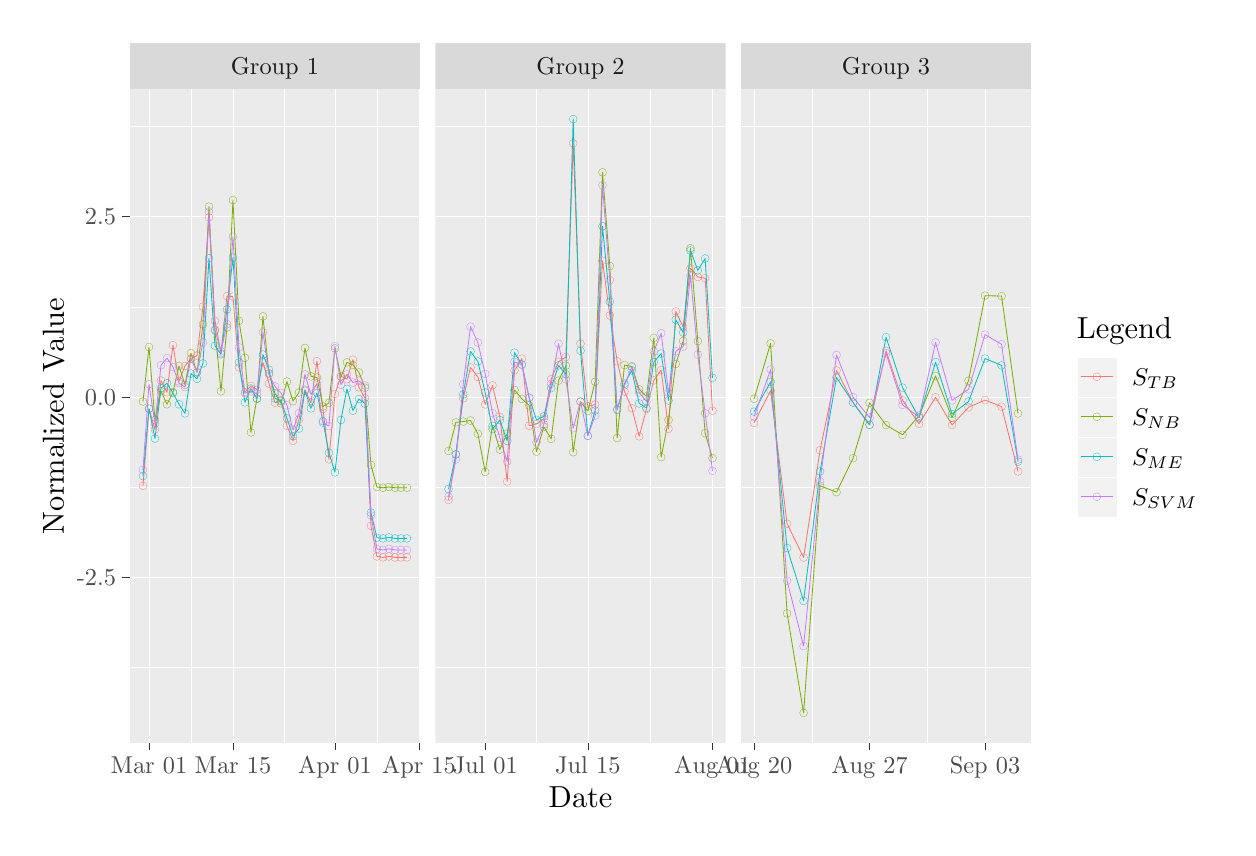
\begin{tikzpicture}[x=1pt,y=1pt]
\definecolor{fillColor}{RGB}{255,255,255}
\path[use as bounding box,fill=fillColor,fill opacity=0.00] (0,0) rectangle (433.62,289.08);
\begin{scope}
\path[clip] (  0.00,  0.00) rectangle (433.62,289.08);
\definecolor{drawColor}{RGB}{255,255,255}
\definecolor{fillColor}{RGB}{255,255,255}

\path[draw=drawColor,line width= 0.1pt,line join=round,line cap=round,fill=fillColor] (  0.00,  0.00) rectangle (433.62,289.08);
\end{scope}
\begin{scope}
\path[clip] ( 36.90, 30.73) rectangle (141.81,266.77);
\definecolor{fillColor}{gray}{0.92}

\path[fill=fillColor] ( 36.90, 30.73) rectangle (141.81,266.77);
\definecolor{drawColor}{RGB}{255,255,255}

\path[draw=drawColor,line width= 0.1pt,line join=round] ( 36.90, 57.88) --
	(141.81, 57.88);

\path[draw=drawColor,line width= 0.1pt,line join=round] ( 36.90,123.08) --
	(141.81,123.08);

\path[draw=drawColor,line width= 0.1pt,line join=round] ( 36.90,188.27) --
	(141.81,188.27);

\path[draw=drawColor,line width= 0.1pt,line join=round] ( 36.90,253.47) --
	(141.81,253.47);

\path[draw=drawColor,line width= 0.1pt,line join=round] ( 59.01, 30.73) --
	( 59.01,266.77);

\path[draw=drawColor,line width= 0.1pt,line join=round] ( 92.61, 30.73) --
	( 92.61,266.77);

\path[draw=drawColor,line width= 0.1pt,line join=round] (126.20, 30.73) --
	(126.20,266.77);

\path[draw=drawColor,line width= 0.1pt,line join=round] ( 36.90, 90.48) --
	(141.81, 90.48);

\path[draw=drawColor,line width= 0.1pt,line join=round] ( 36.90,155.67) --
	(141.81,155.67);

\path[draw=drawColor,line width= 0.1pt,line join=round] ( 36.90,220.87) --
	(141.81,220.87);

\path[draw=drawColor,line width= 0.1pt,line join=round] ( 43.84, 30.73) --
	( 43.84,266.77);

\path[draw=drawColor,line width= 0.1pt,line join=round] ( 74.18, 30.73) --
	( 74.18,266.77);

\path[draw=drawColor,line width= 0.1pt,line join=round] (111.03, 30.73) --
	(111.03,266.77);

\path[draw=drawColor,line width= 0.1pt,line join=round] (141.38, 30.73) --
	(141.38,266.77);
\definecolor{drawColor}{RGB}{248,118,109}

\path[draw=drawColor,line width= 0.3pt,line join=round] ( 41.67,123.51) --
	( 43.84,151.41) --
	( 46.00,143.91) --
	( 48.17,161.57) --
	( 50.34,157.32) --
	( 52.51,174.33) --
	( 54.67,161.28) --
	( 56.84,166.83) --
	( 59.01,169.54) --
	( 61.18,170.59) --
	( 63.34,188.26) --
	( 65.51,220.56) --
	( 67.68,183.15) --
	( 69.85,171.46) --
	( 72.01,192.09) --
	( 74.18,191.87) --
	( 76.35,166.32) --
	( 78.52,157.36) --
	( 80.68,159.65) --
	( 82.85,158.20) --
	( 85.02,168.10) --
	( 87.19,160.50) --
	( 89.35,153.56) --
	( 91.52,154.09) --
	( 93.69,145.21) --
	( 95.86,139.76) --
	( 98.03,147.53) --
	(100.19,158.27) --
	(102.36,153.51) --
	(104.53,168.56) --
	(106.70,151.32) --
	(108.86,133.10) --
	(111.03,156.69) --
	(113.20,163.13) --
	(115.37,162.06) --
	(117.53,169.11) --
	(119.70,159.12) --
	(121.87,155.22) --
	(124.04,109.05) --
	(126.20, 98.01) --
	(128.37, 97.66) --
	(130.54, 98.01) --
	(132.71, 97.66) --
	(134.87, 97.66) --
	(137.04, 97.66);
\definecolor{drawColor}{RGB}{124,174,0}

\path[draw=drawColor,line width= 0.3pt,line join=round] ( 41.67,154.00) --
	( 43.84,173.67) --
	( 46.00,147.28) --
	( 48.17,157.76) --
	( 50.34,152.99) --
	( 52.51,157.36) --
	( 54.67,166.84) --
	( 56.84,159.99) --
	( 59.01,171.49) --
	( 61.18,164.46) --
	( 63.34,181.86) --
	( 65.51,224.40) --
	( 67.68,179.71) --
	( 69.85,157.70) --
	( 72.01,180.75) --
	( 74.18,226.77) --
	( 76.35,183.14) --
	( 78.52,169.80) --
	( 80.68,142.84) --
	( 82.85,155.09) --
	( 85.02,184.76) --
	( 87.19,164.20) --
	( 89.35,157.00) --
	( 91.52,153.34) --
	( 93.69,161.20) --
	( 95.86,154.14) --
	( 98.03,157.24) --
	(100.19,173.34) --
	(102.36,163.11) --
	(104.53,162.64) --
	(106.70,152.19) --
	(108.86,153.48) --
	(111.03,173.21) --
	(113.20,162.98) --
	(115.37,168.14) --
	(117.53,167.19) --
	(119.70,164.51) --
	(121.87,158.96) --
	(124.04,131.04) --
	(126.20,123.09) --
	(128.37,122.83) --
	(130.54,123.10) --
	(132.71,122.85) --
	(134.87,122.84) --
	(137.04,122.85);
\definecolor{drawColor}{RGB}{0,191,196}

\path[draw=drawColor,line width= 0.3pt,line join=round] ( 41.67,127.06) --
	( 43.84,151.36) --
	( 46.00,140.61) --
	( 48.17,158.78) --
	( 50.34,160.58) --
	( 52.51,157.06) --
	( 54.67,152.99) --
	( 56.84,149.71) --
	( 59.01,164.10) --
	( 61.18,162.18) --
	( 63.34,167.76) --
	( 65.51,205.76) --
	( 67.68,174.12) --
	( 69.85,171.07) --
	( 72.01,187.26) --
	( 74.18,205.98) --
	( 76.35,168.11) --
	( 78.52,153.67) --
	( 80.68,158.70) --
	( 82.85,154.96) --
	( 85.02,170.94) --
	( 87.19,165.47) --
	( 89.35,155.17) --
	( 91.52,154.31) --
	( 93.69,147.92) --
	( 95.86,141.44) --
	( 98.03,144.21) --
	(100.19,157.89) --
	(102.36,151.52) --
	(104.53,157.08) --
	(106.70,146.88) --
	(108.86,135.44) --
	(111.03,128.41) --
	(113.20,147.34) --
	(115.37,158.57) --
	(117.53,150.69) --
	(119.70,154.89) --
	(121.87,153.25) --
	(124.04,113.82) --
	(126.20,104.78) --
	(128.37,104.52) --
	(130.54,104.87) --
	(132.71,104.52) --
	(134.87,104.52) --
	(137.04,104.52);
\definecolor{drawColor}{RGB}{199,124,255}

\path[draw=drawColor,line width= 0.3pt,line join=round] ( 41.67,129.31) --
	( 43.84,160.26) --
	( 46.00,145.93) --
	( 48.17,167.10) --
	( 50.34,169.68) --
	( 52.51,166.46) --
	( 54.67,160.64) --
	( 56.84,159.20) --
	( 59.01,169.35) --
	( 61.18,164.70) --
	( 63.34,175.36) --
	( 65.51,222.64) --
	( 67.68,179.93) --
	( 69.85,172.11) --
	( 72.01,181.95) --
	( 74.18,213.53) --
	( 76.35,173.58) --
	( 78.52,157.02) --
	( 80.68,157.66) --
	( 82.85,156.83) --
	( 85.02,178.99) --
	( 87.19,163.89) --
	( 89.35,159.43) --
	( 91.52,157.13) --
	( 93.69,152.62) --
	( 95.86,143.67) --
	( 98.03,149.82) --
	(100.19,163.76) --
	(102.36,156.48) --
	(104.53,160.56) --
	(106.70,146.32) --
	(108.86,145.10) --
	(111.03,174.05) --
	(113.20,160.04) --
	(115.37,163.81) --
	(117.53,160.85) --
	(119.70,161.46) --
	(121.87,159.79) --
	(124.04,112.83) --
	(126.20,100.72) --
	(128.37,100.37) --
	(130.54,100.77) --
	(132.71,100.36) --
	(134.87,100.36) --
	(137.04,100.36);
\definecolor{drawColor}{RGB}{248,118,109}

\path[draw=drawColor,line width= 0.1pt,line join=round,line cap=round] ( 41.67,123.51) circle (  1.43);

\path[draw=drawColor,line width= 0.1pt,line join=round,line cap=round] ( 43.84,151.41) circle (  1.43);

\path[draw=drawColor,line width= 0.1pt,line join=round,line cap=round] ( 46.00,143.91) circle (  1.43);

\path[draw=drawColor,line width= 0.1pt,line join=round,line cap=round] ( 48.17,161.57) circle (  1.43);

\path[draw=drawColor,line width= 0.1pt,line join=round,line cap=round] ( 50.34,157.32) circle (  1.43);

\path[draw=drawColor,line width= 0.1pt,line join=round,line cap=round] ( 52.51,174.33) circle (  1.43);

\path[draw=drawColor,line width= 0.1pt,line join=round,line cap=round] ( 54.67,161.28) circle (  1.43);

\path[draw=drawColor,line width= 0.1pt,line join=round,line cap=round] ( 56.84,166.83) circle (  1.43);

\path[draw=drawColor,line width= 0.1pt,line join=round,line cap=round] ( 59.01,169.54) circle (  1.43);

\path[draw=drawColor,line width= 0.1pt,line join=round,line cap=round] ( 61.18,170.59) circle (  1.43);

\path[draw=drawColor,line width= 0.1pt,line join=round,line cap=round] ( 63.34,188.26) circle (  1.43);

\path[draw=drawColor,line width= 0.1pt,line join=round,line cap=round] ( 65.51,220.56) circle (  1.43);

\path[draw=drawColor,line width= 0.1pt,line join=round,line cap=round] ( 67.68,183.15) circle (  1.43);

\path[draw=drawColor,line width= 0.1pt,line join=round,line cap=round] ( 69.85,171.46) circle (  1.43);

\path[draw=drawColor,line width= 0.1pt,line join=round,line cap=round] ( 72.01,192.09) circle (  1.43);

\path[draw=drawColor,line width= 0.1pt,line join=round,line cap=round] ( 74.18,191.87) circle (  1.43);

\path[draw=drawColor,line width= 0.1pt,line join=round,line cap=round] ( 76.35,166.32) circle (  1.43);

\path[draw=drawColor,line width= 0.1pt,line join=round,line cap=round] ( 78.52,157.36) circle (  1.43);

\path[draw=drawColor,line width= 0.1pt,line join=round,line cap=round] ( 80.68,159.65) circle (  1.43);

\path[draw=drawColor,line width= 0.1pt,line join=round,line cap=round] ( 82.85,158.20) circle (  1.43);

\path[draw=drawColor,line width= 0.1pt,line join=round,line cap=round] ( 85.02,168.10) circle (  1.43);

\path[draw=drawColor,line width= 0.1pt,line join=round,line cap=round] ( 87.19,160.50) circle (  1.43);

\path[draw=drawColor,line width= 0.1pt,line join=round,line cap=round] ( 89.35,153.56) circle (  1.43);

\path[draw=drawColor,line width= 0.1pt,line join=round,line cap=round] ( 91.52,154.09) circle (  1.43);

\path[draw=drawColor,line width= 0.1pt,line join=round,line cap=round] ( 93.69,145.21) circle (  1.43);

\path[draw=drawColor,line width= 0.1pt,line join=round,line cap=round] ( 95.86,139.76) circle (  1.43);

\path[draw=drawColor,line width= 0.1pt,line join=round,line cap=round] ( 98.03,147.53) circle (  1.43);

\path[draw=drawColor,line width= 0.1pt,line join=round,line cap=round] (100.19,158.27) circle (  1.43);

\path[draw=drawColor,line width= 0.1pt,line join=round,line cap=round] (102.36,153.51) circle (  1.43);

\path[draw=drawColor,line width= 0.1pt,line join=round,line cap=round] (104.53,168.56) circle (  1.43);

\path[draw=drawColor,line width= 0.1pt,line join=round,line cap=round] (106.70,151.32) circle (  1.43);

\path[draw=drawColor,line width= 0.1pt,line join=round,line cap=round] (108.86,133.10) circle (  1.43);

\path[draw=drawColor,line width= 0.1pt,line join=round,line cap=round] (111.03,156.69) circle (  1.43);

\path[draw=drawColor,line width= 0.1pt,line join=round,line cap=round] (113.20,163.13) circle (  1.43);

\path[draw=drawColor,line width= 0.1pt,line join=round,line cap=round] (115.37,162.06) circle (  1.43);

\path[draw=drawColor,line width= 0.1pt,line join=round,line cap=round] (117.53,169.11) circle (  1.43);

\path[draw=drawColor,line width= 0.1pt,line join=round,line cap=round] (119.70,159.12) circle (  1.43);

\path[draw=drawColor,line width= 0.1pt,line join=round,line cap=round] (121.87,155.22) circle (  1.43);

\path[draw=drawColor,line width= 0.1pt,line join=round,line cap=round] (124.04,109.05) circle (  1.43);

\path[draw=drawColor,line width= 0.1pt,line join=round,line cap=round] (126.20, 98.01) circle (  1.43);

\path[draw=drawColor,line width= 0.1pt,line join=round,line cap=round] (128.37, 97.66) circle (  1.43);

\path[draw=drawColor,line width= 0.1pt,line join=round,line cap=round] (130.54, 98.01) circle (  1.43);

\path[draw=drawColor,line width= 0.1pt,line join=round,line cap=round] (132.71, 97.66) circle (  1.43);

\path[draw=drawColor,line width= 0.1pt,line join=round,line cap=round] (134.87, 97.66) circle (  1.43);

\path[draw=drawColor,line width= 0.1pt,line join=round,line cap=round] (137.04, 97.66) circle (  1.43);
\definecolor{drawColor}{RGB}{124,174,0}

\path[draw=drawColor,line width= 0.1pt,line join=round,line cap=round] ( 41.67,154.00) circle (  1.43);

\path[draw=drawColor,line width= 0.1pt,line join=round,line cap=round] ( 43.84,173.67) circle (  1.43);

\path[draw=drawColor,line width= 0.1pt,line join=round,line cap=round] ( 46.00,147.28) circle (  1.43);

\path[draw=drawColor,line width= 0.1pt,line join=round,line cap=round] ( 48.17,157.76) circle (  1.43);

\path[draw=drawColor,line width= 0.1pt,line join=round,line cap=round] ( 50.34,152.99) circle (  1.43);

\path[draw=drawColor,line width= 0.1pt,line join=round,line cap=round] ( 52.51,157.36) circle (  1.43);

\path[draw=drawColor,line width= 0.1pt,line join=round,line cap=round] ( 54.67,166.84) circle (  1.43);

\path[draw=drawColor,line width= 0.1pt,line join=round,line cap=round] ( 56.84,159.99) circle (  1.43);

\path[draw=drawColor,line width= 0.1pt,line join=round,line cap=round] ( 59.01,171.49) circle (  1.43);

\path[draw=drawColor,line width= 0.1pt,line join=round,line cap=round] ( 61.18,164.46) circle (  1.43);

\path[draw=drawColor,line width= 0.1pt,line join=round,line cap=round] ( 63.34,181.86) circle (  1.43);

\path[draw=drawColor,line width= 0.1pt,line join=round,line cap=round] ( 65.51,224.40) circle (  1.43);

\path[draw=drawColor,line width= 0.1pt,line join=round,line cap=round] ( 67.68,179.71) circle (  1.43);

\path[draw=drawColor,line width= 0.1pt,line join=round,line cap=round] ( 69.85,157.70) circle (  1.43);

\path[draw=drawColor,line width= 0.1pt,line join=round,line cap=round] ( 72.01,180.75) circle (  1.43);

\path[draw=drawColor,line width= 0.1pt,line join=round,line cap=round] ( 74.18,226.77) circle (  1.43);

\path[draw=drawColor,line width= 0.1pt,line join=round,line cap=round] ( 76.35,183.14) circle (  1.43);

\path[draw=drawColor,line width= 0.1pt,line join=round,line cap=round] ( 78.52,169.80) circle (  1.43);

\path[draw=drawColor,line width= 0.1pt,line join=round,line cap=round] ( 80.68,142.84) circle (  1.43);

\path[draw=drawColor,line width= 0.1pt,line join=round,line cap=round] ( 82.85,155.09) circle (  1.43);

\path[draw=drawColor,line width= 0.1pt,line join=round,line cap=round] ( 85.02,184.76) circle (  1.43);

\path[draw=drawColor,line width= 0.1pt,line join=round,line cap=round] ( 87.19,164.20) circle (  1.43);

\path[draw=drawColor,line width= 0.1pt,line join=round,line cap=round] ( 89.35,157.00) circle (  1.43);

\path[draw=drawColor,line width= 0.1pt,line join=round,line cap=round] ( 91.52,153.34) circle (  1.43);

\path[draw=drawColor,line width= 0.1pt,line join=round,line cap=round] ( 93.69,161.20) circle (  1.43);

\path[draw=drawColor,line width= 0.1pt,line join=round,line cap=round] ( 95.86,154.14) circle (  1.43);

\path[draw=drawColor,line width= 0.1pt,line join=round,line cap=round] ( 98.03,157.24) circle (  1.43);

\path[draw=drawColor,line width= 0.1pt,line join=round,line cap=round] (100.19,173.34) circle (  1.43);

\path[draw=drawColor,line width= 0.1pt,line join=round,line cap=round] (102.36,163.11) circle (  1.43);

\path[draw=drawColor,line width= 0.1pt,line join=round,line cap=round] (104.53,162.64) circle (  1.43);

\path[draw=drawColor,line width= 0.1pt,line join=round,line cap=round] (106.70,152.19) circle (  1.43);

\path[draw=drawColor,line width= 0.1pt,line join=round,line cap=round] (108.86,153.48) circle (  1.43);

\path[draw=drawColor,line width= 0.1pt,line join=round,line cap=round] (111.03,173.21) circle (  1.43);

\path[draw=drawColor,line width= 0.1pt,line join=round,line cap=round] (113.20,162.98) circle (  1.43);

\path[draw=drawColor,line width= 0.1pt,line join=round,line cap=round] (115.37,168.14) circle (  1.43);

\path[draw=drawColor,line width= 0.1pt,line join=round,line cap=round] (117.53,167.19) circle (  1.43);

\path[draw=drawColor,line width= 0.1pt,line join=round,line cap=round] (119.70,164.51) circle (  1.43);

\path[draw=drawColor,line width= 0.1pt,line join=round,line cap=round] (121.87,158.96) circle (  1.43);

\path[draw=drawColor,line width= 0.1pt,line join=round,line cap=round] (124.04,131.04) circle (  1.43);

\path[draw=drawColor,line width= 0.1pt,line join=round,line cap=round] (126.20,123.09) circle (  1.43);

\path[draw=drawColor,line width= 0.1pt,line join=round,line cap=round] (128.37,122.83) circle (  1.43);

\path[draw=drawColor,line width= 0.1pt,line join=round,line cap=round] (130.54,123.10) circle (  1.43);

\path[draw=drawColor,line width= 0.1pt,line join=round,line cap=round] (132.71,122.85) circle (  1.43);

\path[draw=drawColor,line width= 0.1pt,line join=round,line cap=round] (134.87,122.84) circle (  1.43);

\path[draw=drawColor,line width= 0.1pt,line join=round,line cap=round] (137.04,122.85) circle (  1.43);
\definecolor{drawColor}{RGB}{0,191,196}

\path[draw=drawColor,line width= 0.1pt,line join=round,line cap=round] ( 41.67,127.06) circle (  1.43);

\path[draw=drawColor,line width= 0.1pt,line join=round,line cap=round] ( 43.84,151.36) circle (  1.43);

\path[draw=drawColor,line width= 0.1pt,line join=round,line cap=round] ( 46.00,140.61) circle (  1.43);

\path[draw=drawColor,line width= 0.1pt,line join=round,line cap=round] ( 48.17,158.78) circle (  1.43);

\path[draw=drawColor,line width= 0.1pt,line join=round,line cap=round] ( 50.34,160.58) circle (  1.43);

\path[draw=drawColor,line width= 0.1pt,line join=round,line cap=round] ( 52.51,157.06) circle (  1.43);

\path[draw=drawColor,line width= 0.1pt,line join=round,line cap=round] ( 54.67,152.99) circle (  1.43);

\path[draw=drawColor,line width= 0.1pt,line join=round,line cap=round] ( 56.84,149.71) circle (  1.43);

\path[draw=drawColor,line width= 0.1pt,line join=round,line cap=round] ( 59.01,164.10) circle (  1.43);

\path[draw=drawColor,line width= 0.1pt,line join=round,line cap=round] ( 61.18,162.18) circle (  1.43);

\path[draw=drawColor,line width= 0.1pt,line join=round,line cap=round] ( 63.34,167.76) circle (  1.43);

\path[draw=drawColor,line width= 0.1pt,line join=round,line cap=round] ( 65.51,205.76) circle (  1.43);

\path[draw=drawColor,line width= 0.1pt,line join=round,line cap=round] ( 67.68,174.12) circle (  1.43);

\path[draw=drawColor,line width= 0.1pt,line join=round,line cap=round] ( 69.85,171.07) circle (  1.43);

\path[draw=drawColor,line width= 0.1pt,line join=round,line cap=round] ( 72.01,187.26) circle (  1.43);

\path[draw=drawColor,line width= 0.1pt,line join=round,line cap=round] ( 74.18,205.98) circle (  1.43);

\path[draw=drawColor,line width= 0.1pt,line join=round,line cap=round] ( 76.35,168.11) circle (  1.43);

\path[draw=drawColor,line width= 0.1pt,line join=round,line cap=round] ( 78.52,153.67) circle (  1.43);

\path[draw=drawColor,line width= 0.1pt,line join=round,line cap=round] ( 80.68,158.70) circle (  1.43);

\path[draw=drawColor,line width= 0.1pt,line join=round,line cap=round] ( 82.85,154.96) circle (  1.43);

\path[draw=drawColor,line width= 0.1pt,line join=round,line cap=round] ( 85.02,170.94) circle (  1.43);

\path[draw=drawColor,line width= 0.1pt,line join=round,line cap=round] ( 87.19,165.47) circle (  1.43);

\path[draw=drawColor,line width= 0.1pt,line join=round,line cap=round] ( 89.35,155.17) circle (  1.43);

\path[draw=drawColor,line width= 0.1pt,line join=round,line cap=round] ( 91.52,154.31) circle (  1.43);

\path[draw=drawColor,line width= 0.1pt,line join=round,line cap=round] ( 93.69,147.92) circle (  1.43);

\path[draw=drawColor,line width= 0.1pt,line join=round,line cap=round] ( 95.86,141.44) circle (  1.43);

\path[draw=drawColor,line width= 0.1pt,line join=round,line cap=round] ( 98.03,144.21) circle (  1.43);

\path[draw=drawColor,line width= 0.1pt,line join=round,line cap=round] (100.19,157.89) circle (  1.43);

\path[draw=drawColor,line width= 0.1pt,line join=round,line cap=round] (102.36,151.52) circle (  1.43);

\path[draw=drawColor,line width= 0.1pt,line join=round,line cap=round] (104.53,157.08) circle (  1.43);

\path[draw=drawColor,line width= 0.1pt,line join=round,line cap=round] (106.70,146.88) circle (  1.43);

\path[draw=drawColor,line width= 0.1pt,line join=round,line cap=round] (108.86,135.44) circle (  1.43);

\path[draw=drawColor,line width= 0.1pt,line join=round,line cap=round] (111.03,128.41) circle (  1.43);

\path[draw=drawColor,line width= 0.1pt,line join=round,line cap=round] (113.20,147.34) circle (  1.43);

\path[draw=drawColor,line width= 0.1pt,line join=round,line cap=round] (115.37,158.57) circle (  1.43);

\path[draw=drawColor,line width= 0.1pt,line join=round,line cap=round] (117.53,150.69) circle (  1.43);

\path[draw=drawColor,line width= 0.1pt,line join=round,line cap=round] (119.70,154.89) circle (  1.43);

\path[draw=drawColor,line width= 0.1pt,line join=round,line cap=round] (121.87,153.25) circle (  1.43);

\path[draw=drawColor,line width= 0.1pt,line join=round,line cap=round] (124.04,113.82) circle (  1.43);

\path[draw=drawColor,line width= 0.1pt,line join=round,line cap=round] (126.20,104.78) circle (  1.43);

\path[draw=drawColor,line width= 0.1pt,line join=round,line cap=round] (128.37,104.52) circle (  1.43);

\path[draw=drawColor,line width= 0.1pt,line join=round,line cap=round] (130.54,104.87) circle (  1.43);

\path[draw=drawColor,line width= 0.1pt,line join=round,line cap=round] (132.71,104.52) circle (  1.43);

\path[draw=drawColor,line width= 0.1pt,line join=round,line cap=round] (134.87,104.52) circle (  1.43);

\path[draw=drawColor,line width= 0.1pt,line join=round,line cap=round] (137.04,104.52) circle (  1.43);
\definecolor{drawColor}{RGB}{199,124,255}

\path[draw=drawColor,line width= 0.1pt,line join=round,line cap=round] ( 41.67,129.31) circle (  1.43);

\path[draw=drawColor,line width= 0.1pt,line join=round,line cap=round] ( 43.84,160.26) circle (  1.43);

\path[draw=drawColor,line width= 0.1pt,line join=round,line cap=round] ( 46.00,145.93) circle (  1.43);

\path[draw=drawColor,line width= 0.1pt,line join=round,line cap=round] ( 48.17,167.10) circle (  1.43);

\path[draw=drawColor,line width= 0.1pt,line join=round,line cap=round] ( 50.34,169.68) circle (  1.43);

\path[draw=drawColor,line width= 0.1pt,line join=round,line cap=round] ( 52.51,166.46) circle (  1.43);

\path[draw=drawColor,line width= 0.1pt,line join=round,line cap=round] ( 54.67,160.64) circle (  1.43);

\path[draw=drawColor,line width= 0.1pt,line join=round,line cap=round] ( 56.84,159.20) circle (  1.43);

\path[draw=drawColor,line width= 0.1pt,line join=round,line cap=round] ( 59.01,169.35) circle (  1.43);

\path[draw=drawColor,line width= 0.1pt,line join=round,line cap=round] ( 61.18,164.70) circle (  1.43);

\path[draw=drawColor,line width= 0.1pt,line join=round,line cap=round] ( 63.34,175.36) circle (  1.43);

\path[draw=drawColor,line width= 0.1pt,line join=round,line cap=round] ( 65.51,222.64) circle (  1.43);

\path[draw=drawColor,line width= 0.1pt,line join=round,line cap=round] ( 67.68,179.93) circle (  1.43);

\path[draw=drawColor,line width= 0.1pt,line join=round,line cap=round] ( 69.85,172.11) circle (  1.43);

\path[draw=drawColor,line width= 0.1pt,line join=round,line cap=round] ( 72.01,181.95) circle (  1.43);

\path[draw=drawColor,line width= 0.1pt,line join=round,line cap=round] ( 74.18,213.53) circle (  1.43);

\path[draw=drawColor,line width= 0.1pt,line join=round,line cap=round] ( 76.35,173.58) circle (  1.43);

\path[draw=drawColor,line width= 0.1pt,line join=round,line cap=round] ( 78.52,157.02) circle (  1.43);

\path[draw=drawColor,line width= 0.1pt,line join=round,line cap=round] ( 80.68,157.66) circle (  1.43);

\path[draw=drawColor,line width= 0.1pt,line join=round,line cap=round] ( 82.85,156.83) circle (  1.43);

\path[draw=drawColor,line width= 0.1pt,line join=round,line cap=round] ( 85.02,178.99) circle (  1.43);

\path[draw=drawColor,line width= 0.1pt,line join=round,line cap=round] ( 87.19,163.89) circle (  1.43);

\path[draw=drawColor,line width= 0.1pt,line join=round,line cap=round] ( 89.35,159.43) circle (  1.43);

\path[draw=drawColor,line width= 0.1pt,line join=round,line cap=round] ( 91.52,157.13) circle (  1.43);

\path[draw=drawColor,line width= 0.1pt,line join=round,line cap=round] ( 93.69,152.62) circle (  1.43);

\path[draw=drawColor,line width= 0.1pt,line join=round,line cap=round] ( 95.86,143.67) circle (  1.43);

\path[draw=drawColor,line width= 0.1pt,line join=round,line cap=round] ( 98.03,149.82) circle (  1.43);

\path[draw=drawColor,line width= 0.1pt,line join=round,line cap=round] (100.19,163.76) circle (  1.43);

\path[draw=drawColor,line width= 0.1pt,line join=round,line cap=round] (102.36,156.48) circle (  1.43);

\path[draw=drawColor,line width= 0.1pt,line join=round,line cap=round] (104.53,160.56) circle (  1.43);

\path[draw=drawColor,line width= 0.1pt,line join=round,line cap=round] (106.70,146.32) circle (  1.43);

\path[draw=drawColor,line width= 0.1pt,line join=round,line cap=round] (108.86,145.10) circle (  1.43);

\path[draw=drawColor,line width= 0.1pt,line join=round,line cap=round] (111.03,174.05) circle (  1.43);

\path[draw=drawColor,line width= 0.1pt,line join=round,line cap=round] (113.20,160.04) circle (  1.43);

\path[draw=drawColor,line width= 0.1pt,line join=round,line cap=round] (115.37,163.81) circle (  1.43);

\path[draw=drawColor,line width= 0.1pt,line join=round,line cap=round] (117.53,160.85) circle (  1.43);

\path[draw=drawColor,line width= 0.1pt,line join=round,line cap=round] (119.70,161.46) circle (  1.43);

\path[draw=drawColor,line width= 0.1pt,line join=round,line cap=round] (121.87,159.79) circle (  1.43);

\path[draw=drawColor,line width= 0.1pt,line join=round,line cap=round] (124.04,112.83) circle (  1.43);

\path[draw=drawColor,line width= 0.1pt,line join=round,line cap=round] (126.20,100.72) circle (  1.43);

\path[draw=drawColor,line width= 0.1pt,line join=round,line cap=round] (128.37,100.37) circle (  1.43);

\path[draw=drawColor,line width= 0.1pt,line join=round,line cap=round] (130.54,100.77) circle (  1.43);

\path[draw=drawColor,line width= 0.1pt,line join=round,line cap=round] (132.71,100.36) circle (  1.43);

\path[draw=drawColor,line width= 0.1pt,line join=round,line cap=round] (134.87,100.36) circle (  1.43);

\path[draw=drawColor,line width= 0.1pt,line join=round,line cap=round] (137.04,100.36) circle (  1.43);
\end{scope}
\begin{scope}
\path[clip] (147.31, 30.73) rectangle (252.22,266.77);
\definecolor{fillColor}{gray}{0.92}

\path[fill=fillColor] (147.31, 30.73) rectangle (252.22,266.77);
\definecolor{drawColor}{RGB}{255,255,255}

\path[draw=drawColor,line width= 0.1pt,line join=round] (147.31, 57.88) --
	(252.22, 57.88);

\path[draw=drawColor,line width= 0.1pt,line join=round] (147.31,123.08) --
	(252.22,123.08);

\path[draw=drawColor,line width= 0.1pt,line join=round] (147.31,188.27) --
	(252.22,188.27);

\path[draw=drawColor,line width= 0.1pt,line join=round] (147.31,253.47) --
	(252.22,253.47);

\path[draw=drawColor,line width= 0.1pt,line join=round] (183.87, 30.73) --
	(183.87,266.77);

\path[draw=drawColor,line width= 0.1pt,line join=round] (224.93, 30.73) --
	(224.93,266.77);

\path[draw=drawColor,line width= 0.1pt,line join=round] (147.31, 90.48) --
	(252.22, 90.48);

\path[draw=drawColor,line width= 0.1pt,line join=round] (147.31,155.67) --
	(252.22,155.67);

\path[draw=drawColor,line width= 0.1pt,line join=round] (147.31,220.87) --
	(252.22,220.87);

\path[draw=drawColor,line width= 0.1pt,line join=round] (165.32, 30.73) --
	(165.32,266.77);

\path[draw=drawColor,line width= 0.1pt,line join=round] (202.41, 30.73) --
	(202.41,266.77);

\path[draw=drawColor,line width= 0.1pt,line join=round] (247.45, 30.73) --
	(247.45,266.77);
\definecolor{drawColor}{RGB}{248,118,109}

\path[draw=drawColor,line width= 0.3pt,line join=round] (152.08,118.43) --
	(154.73,134.88) --
	(157.38,155.12) --
	(160.03,166.28) --
	(162.68,162.86) --
	(165.32,152.93) --
	(167.97,159.82) --
	(170.62,148.45) --
	(173.27,125.08) --
	(175.92,165.21) --
	(178.57,169.49) --
	(181.22,145.24) --
	(183.87,145.87) --
	(186.52,147.74) --
	(189.17,162.06) --
	(191.82,168.35) --
	(194.47,170.03) --
	(197.12,247.31) --
	(199.76,174.90) --
	(202.41,152.22) --
	(205.06,152.89) --
	(207.71,204.87) --
	(210.36,185.09) --
	(213.01,168.54) --
	(215.66,157.61) --
	(218.31,151.59) --
	(220.96,141.42) --
	(223.61,151.30) --
	(226.26,161.64) --
	(228.91,165.37) --
	(231.56,144.11) --
	(234.20,186.59) --
	(236.85,180.92) --
	(239.50,202.13) --
	(242.15,198.99) --
	(244.80,198.57) --
	(247.45,150.67);
\definecolor{drawColor}{RGB}{124,174,0}

\path[draw=drawColor,line width= 0.3pt,line join=round] (152.08,136.14) --
	(154.73,146.46) --
	(157.38,146.74) --
	(160.03,147.13) --
	(162.68,142.33) --
	(165.32,128.54) --
	(167.97,145.20) --
	(170.62,136.63) --
	(173.27,142.39) --
	(175.92,158.17) --
	(178.57,154.95) --
	(181.22,152.58) --
	(183.87,135.88) --
	(186.52,144.84) --
	(189.17,140.48) --
	(191.82,161.54) --
	(194.47,166.91) --
	(197.12,135.68) --
	(199.76,153.90) --
	(202.41,150.53) --
	(205.06,161.12) --
	(207.71,236.79) --
	(210.36,202.95) --
	(213.01,140.80) --
	(215.66,167.15) --
	(218.31,166.71) --
	(220.96,158.40) --
	(223.61,155.85) --
	(226.26,176.99) --
	(228.91,133.88) --
	(231.56,147.31) --
	(234.20,167.57) --
	(236.85,175.87) --
	(239.50,209.36) --
	(242.15,175.81) --
	(244.80,142.53) --
	(247.45,133.53);
\definecolor{drawColor}{RGB}{0,191,196}

\path[draw=drawColor,line width= 0.3pt,line join=round] (152.08,122.37) --
	(154.73,134.90) --
	(157.38,156.54) --
	(160.03,172.10) --
	(162.68,168.45) --
	(165.32,157.25) --
	(167.97,144.03) --
	(170.62,147.28) --
	(173.27,139.70) --
	(175.92,171.66) --
	(178.57,167.40) --
	(181.22,155.32) --
	(183.87,147.34) --
	(186.52,148.67) --
	(189.17,158.85) --
	(191.82,167.04) --
	(194.47,163.81) --
	(197.12,256.04) --
	(199.76,172.34) --
	(202.41,141.64) --
	(205.06,150.74) --
	(207.71,217.31) --
	(210.36,190.06) --
	(213.01,151.13) --
	(215.66,160.45) --
	(218.31,165.21) --
	(220.96,153.31) --
	(223.61,151.66) --
	(226.26,168.24) --
	(228.91,171.33) --
	(231.56,154.37) --
	(234.20,183.58) --
	(236.85,178.92) --
	(239.50,208.55) --
	(242.15,201.39) --
	(244.80,205.66) --
	(247.45,162.52);
\definecolor{drawColor}{RGB}{199,124,255}

\path[draw=drawColor,line width= 0.3pt,line join=round] (152.08,119.60) --
	(154.73,133.06) --
	(157.38,160.18) --
	(160.03,181.04) --
	(162.68,175.30) --
	(165.32,163.98) --
	(167.97,149.83) --
	(170.62,140.87) --
	(173.27,132.29) --
	(175.92,168.33) --
	(178.57,167.25) --
	(181.22,155.38) --
	(183.87,139.22) --
	(186.52,145.68) --
	(189.17,160.34) --
	(191.82,174.89) --
	(194.47,162.06) --
	(197.12,144.33) --
	(199.76,154.03) --
	(202.41,141.51) --
	(205.06,148.89) --
	(207.71,232.12) --
	(210.36,197.91) --
	(213.01,150.94) --
	(215.66,159.90) --
	(218.31,166.47) --
	(220.96,157.23) --
	(223.61,154.04) --
	(226.26,172.08) --
	(228.91,178.68) --
	(231.56,157.17) --
	(234.20,172.14) --
	(236.85,173.81) --
	(239.50,199.55) --
	(242.15,170.96) --
	(244.80,149.76) --
	(247.45,128.96);
\definecolor{drawColor}{RGB}{248,118,109}

\path[draw=drawColor,line width= 0.1pt,line join=round,line cap=round] (152.08,118.43) circle (  1.43);

\path[draw=drawColor,line width= 0.1pt,line join=round,line cap=round] (154.73,134.88) circle (  1.43);

\path[draw=drawColor,line width= 0.1pt,line join=round,line cap=round] (157.38,155.12) circle (  1.43);

\path[draw=drawColor,line width= 0.1pt,line join=round,line cap=round] (160.03,166.28) circle (  1.43);

\path[draw=drawColor,line width= 0.1pt,line join=round,line cap=round] (162.68,162.86) circle (  1.43);

\path[draw=drawColor,line width= 0.1pt,line join=round,line cap=round] (165.32,152.93) circle (  1.43);

\path[draw=drawColor,line width= 0.1pt,line join=round,line cap=round] (167.97,159.82) circle (  1.43);

\path[draw=drawColor,line width= 0.1pt,line join=round,line cap=round] (170.62,148.45) circle (  1.43);

\path[draw=drawColor,line width= 0.1pt,line join=round,line cap=round] (173.27,125.08) circle (  1.43);

\path[draw=drawColor,line width= 0.1pt,line join=round,line cap=round] (175.92,165.21) circle (  1.43);

\path[draw=drawColor,line width= 0.1pt,line join=round,line cap=round] (178.57,169.49) circle (  1.43);

\path[draw=drawColor,line width= 0.1pt,line join=round,line cap=round] (181.22,145.24) circle (  1.43);

\path[draw=drawColor,line width= 0.1pt,line join=round,line cap=round] (183.87,145.87) circle (  1.43);

\path[draw=drawColor,line width= 0.1pt,line join=round,line cap=round] (186.52,147.74) circle (  1.43);

\path[draw=drawColor,line width= 0.1pt,line join=round,line cap=round] (189.17,162.06) circle (  1.43);

\path[draw=drawColor,line width= 0.1pt,line join=round,line cap=round] (191.82,168.35) circle (  1.43);

\path[draw=drawColor,line width= 0.1pt,line join=round,line cap=round] (194.47,170.03) circle (  1.43);

\path[draw=drawColor,line width= 0.1pt,line join=round,line cap=round] (197.12,247.31) circle (  1.43);

\path[draw=drawColor,line width= 0.1pt,line join=round,line cap=round] (199.76,174.90) circle (  1.43);

\path[draw=drawColor,line width= 0.1pt,line join=round,line cap=round] (202.41,152.22) circle (  1.43);

\path[draw=drawColor,line width= 0.1pt,line join=round,line cap=round] (205.06,152.89) circle (  1.43);

\path[draw=drawColor,line width= 0.1pt,line join=round,line cap=round] (207.71,204.87) circle (  1.43);

\path[draw=drawColor,line width= 0.1pt,line join=round,line cap=round] (210.36,185.09) circle (  1.43);

\path[draw=drawColor,line width= 0.1pt,line join=round,line cap=round] (213.01,168.54) circle (  1.43);

\path[draw=drawColor,line width= 0.1pt,line join=round,line cap=round] (215.66,157.61) circle (  1.43);

\path[draw=drawColor,line width= 0.1pt,line join=round,line cap=round] (218.31,151.59) circle (  1.43);

\path[draw=drawColor,line width= 0.1pt,line join=round,line cap=round] (220.96,141.42) circle (  1.43);

\path[draw=drawColor,line width= 0.1pt,line join=round,line cap=round] (223.61,151.30) circle (  1.43);

\path[draw=drawColor,line width= 0.1pt,line join=round,line cap=round] (226.26,161.64) circle (  1.43);

\path[draw=drawColor,line width= 0.1pt,line join=round,line cap=round] (228.91,165.37) circle (  1.43);

\path[draw=drawColor,line width= 0.1pt,line join=round,line cap=round] (231.56,144.11) circle (  1.43);

\path[draw=drawColor,line width= 0.1pt,line join=round,line cap=round] (234.20,186.59) circle (  1.43);

\path[draw=drawColor,line width= 0.1pt,line join=round,line cap=round] (236.85,180.92) circle (  1.43);

\path[draw=drawColor,line width= 0.1pt,line join=round,line cap=round] (239.50,202.13) circle (  1.43);

\path[draw=drawColor,line width= 0.1pt,line join=round,line cap=round] (242.15,198.99) circle (  1.43);

\path[draw=drawColor,line width= 0.1pt,line join=round,line cap=round] (244.80,198.57) circle (  1.43);

\path[draw=drawColor,line width= 0.1pt,line join=round,line cap=round] (247.45,150.67) circle (  1.43);
\definecolor{drawColor}{RGB}{124,174,0}

\path[draw=drawColor,line width= 0.1pt,line join=round,line cap=round] (152.08,136.14) circle (  1.43);

\path[draw=drawColor,line width= 0.1pt,line join=round,line cap=round] (154.73,146.46) circle (  1.43);

\path[draw=drawColor,line width= 0.1pt,line join=round,line cap=round] (157.38,146.74) circle (  1.43);

\path[draw=drawColor,line width= 0.1pt,line join=round,line cap=round] (160.03,147.13) circle (  1.43);

\path[draw=drawColor,line width= 0.1pt,line join=round,line cap=round] (162.68,142.33) circle (  1.43);

\path[draw=drawColor,line width= 0.1pt,line join=round,line cap=round] (165.32,128.54) circle (  1.43);

\path[draw=drawColor,line width= 0.1pt,line join=round,line cap=round] (167.97,145.20) circle (  1.43);

\path[draw=drawColor,line width= 0.1pt,line join=round,line cap=round] (170.62,136.63) circle (  1.43);

\path[draw=drawColor,line width= 0.1pt,line join=round,line cap=round] (173.27,142.39) circle (  1.43);

\path[draw=drawColor,line width= 0.1pt,line join=round,line cap=round] (175.92,158.17) circle (  1.43);

\path[draw=drawColor,line width= 0.1pt,line join=round,line cap=round] (178.57,154.95) circle (  1.43);

\path[draw=drawColor,line width= 0.1pt,line join=round,line cap=round] (181.22,152.58) circle (  1.43);

\path[draw=drawColor,line width= 0.1pt,line join=round,line cap=round] (183.87,135.88) circle (  1.43);

\path[draw=drawColor,line width= 0.1pt,line join=round,line cap=round] (186.52,144.84) circle (  1.43);

\path[draw=drawColor,line width= 0.1pt,line join=round,line cap=round] (189.17,140.48) circle (  1.43);

\path[draw=drawColor,line width= 0.1pt,line join=round,line cap=round] (191.82,161.54) circle (  1.43);

\path[draw=drawColor,line width= 0.1pt,line join=round,line cap=round] (194.47,166.91) circle (  1.43);

\path[draw=drawColor,line width= 0.1pt,line join=round,line cap=round] (197.12,135.68) circle (  1.43);

\path[draw=drawColor,line width= 0.1pt,line join=round,line cap=round] (199.76,153.90) circle (  1.43);

\path[draw=drawColor,line width= 0.1pt,line join=round,line cap=round] (202.41,150.53) circle (  1.43);

\path[draw=drawColor,line width= 0.1pt,line join=round,line cap=round] (205.06,161.12) circle (  1.43);

\path[draw=drawColor,line width= 0.1pt,line join=round,line cap=round] (207.71,236.79) circle (  1.43);

\path[draw=drawColor,line width= 0.1pt,line join=round,line cap=round] (210.36,202.95) circle (  1.43);

\path[draw=drawColor,line width= 0.1pt,line join=round,line cap=round] (213.01,140.80) circle (  1.43);

\path[draw=drawColor,line width= 0.1pt,line join=round,line cap=round] (215.66,167.15) circle (  1.43);

\path[draw=drawColor,line width= 0.1pt,line join=round,line cap=round] (218.31,166.71) circle (  1.43);

\path[draw=drawColor,line width= 0.1pt,line join=round,line cap=round] (220.96,158.40) circle (  1.43);

\path[draw=drawColor,line width= 0.1pt,line join=round,line cap=round] (223.61,155.85) circle (  1.43);

\path[draw=drawColor,line width= 0.1pt,line join=round,line cap=round] (226.26,176.99) circle (  1.43);

\path[draw=drawColor,line width= 0.1pt,line join=round,line cap=round] (228.91,133.88) circle (  1.43);

\path[draw=drawColor,line width= 0.1pt,line join=round,line cap=round] (231.56,147.31) circle (  1.43);

\path[draw=drawColor,line width= 0.1pt,line join=round,line cap=round] (234.20,167.57) circle (  1.43);

\path[draw=drawColor,line width= 0.1pt,line join=round,line cap=round] (236.85,175.87) circle (  1.43);

\path[draw=drawColor,line width= 0.1pt,line join=round,line cap=round] (239.50,209.36) circle (  1.43);

\path[draw=drawColor,line width= 0.1pt,line join=round,line cap=round] (242.15,175.81) circle (  1.43);

\path[draw=drawColor,line width= 0.1pt,line join=round,line cap=round] (244.80,142.53) circle (  1.43);

\path[draw=drawColor,line width= 0.1pt,line join=round,line cap=round] (247.45,133.53) circle (  1.43);
\definecolor{drawColor}{RGB}{0,191,196}

\path[draw=drawColor,line width= 0.1pt,line join=round,line cap=round] (152.08,122.37) circle (  1.43);

\path[draw=drawColor,line width= 0.1pt,line join=round,line cap=round] (154.73,134.90) circle (  1.43);

\path[draw=drawColor,line width= 0.1pt,line join=round,line cap=round] (157.38,156.54) circle (  1.43);

\path[draw=drawColor,line width= 0.1pt,line join=round,line cap=round] (160.03,172.10) circle (  1.43);

\path[draw=drawColor,line width= 0.1pt,line join=round,line cap=round] (162.68,168.45) circle (  1.43);

\path[draw=drawColor,line width= 0.1pt,line join=round,line cap=round] (165.32,157.25) circle (  1.43);

\path[draw=drawColor,line width= 0.1pt,line join=round,line cap=round] (167.97,144.03) circle (  1.43);

\path[draw=drawColor,line width= 0.1pt,line join=round,line cap=round] (170.62,147.28) circle (  1.43);

\path[draw=drawColor,line width= 0.1pt,line join=round,line cap=round] (173.27,139.70) circle (  1.43);

\path[draw=drawColor,line width= 0.1pt,line join=round,line cap=round] (175.92,171.66) circle (  1.43);

\path[draw=drawColor,line width= 0.1pt,line join=round,line cap=round] (178.57,167.40) circle (  1.43);

\path[draw=drawColor,line width= 0.1pt,line join=round,line cap=round] (181.22,155.32) circle (  1.43);

\path[draw=drawColor,line width= 0.1pt,line join=round,line cap=round] (183.87,147.34) circle (  1.43);

\path[draw=drawColor,line width= 0.1pt,line join=round,line cap=round] (186.52,148.67) circle (  1.43);

\path[draw=drawColor,line width= 0.1pt,line join=round,line cap=round] (189.17,158.85) circle (  1.43);

\path[draw=drawColor,line width= 0.1pt,line join=round,line cap=round] (191.82,167.04) circle (  1.43);

\path[draw=drawColor,line width= 0.1pt,line join=round,line cap=round] (194.47,163.81) circle (  1.43);

\path[draw=drawColor,line width= 0.1pt,line join=round,line cap=round] (197.12,256.04) circle (  1.43);

\path[draw=drawColor,line width= 0.1pt,line join=round,line cap=round] (199.76,172.34) circle (  1.43);

\path[draw=drawColor,line width= 0.1pt,line join=round,line cap=round] (202.41,141.64) circle (  1.43);

\path[draw=drawColor,line width= 0.1pt,line join=round,line cap=round] (205.06,150.74) circle (  1.43);

\path[draw=drawColor,line width= 0.1pt,line join=round,line cap=round] (207.71,217.31) circle (  1.43);

\path[draw=drawColor,line width= 0.1pt,line join=round,line cap=round] (210.36,190.06) circle (  1.43);

\path[draw=drawColor,line width= 0.1pt,line join=round,line cap=round] (213.01,151.13) circle (  1.43);

\path[draw=drawColor,line width= 0.1pt,line join=round,line cap=round] (215.66,160.45) circle (  1.43);

\path[draw=drawColor,line width= 0.1pt,line join=round,line cap=round] (218.31,165.21) circle (  1.43);

\path[draw=drawColor,line width= 0.1pt,line join=round,line cap=round] (220.96,153.31) circle (  1.43);

\path[draw=drawColor,line width= 0.1pt,line join=round,line cap=round] (223.61,151.66) circle (  1.43);

\path[draw=drawColor,line width= 0.1pt,line join=round,line cap=round] (226.26,168.24) circle (  1.43);

\path[draw=drawColor,line width= 0.1pt,line join=round,line cap=round] (228.91,171.33) circle (  1.43);

\path[draw=drawColor,line width= 0.1pt,line join=round,line cap=round] (231.56,154.37) circle (  1.43);

\path[draw=drawColor,line width= 0.1pt,line join=round,line cap=round] (234.20,183.58) circle (  1.43);

\path[draw=drawColor,line width= 0.1pt,line join=round,line cap=round] (236.85,178.92) circle (  1.43);

\path[draw=drawColor,line width= 0.1pt,line join=round,line cap=round] (239.50,208.55) circle (  1.43);

\path[draw=drawColor,line width= 0.1pt,line join=round,line cap=round] (242.15,201.39) circle (  1.43);

\path[draw=drawColor,line width= 0.1pt,line join=round,line cap=round] (244.80,205.66) circle (  1.43);

\path[draw=drawColor,line width= 0.1pt,line join=round,line cap=round] (247.45,162.52) circle (  1.43);
\definecolor{drawColor}{RGB}{199,124,255}

\path[draw=drawColor,line width= 0.1pt,line join=round,line cap=round] (152.08,119.60) circle (  1.43);

\path[draw=drawColor,line width= 0.1pt,line join=round,line cap=round] (154.73,133.06) circle (  1.43);

\path[draw=drawColor,line width= 0.1pt,line join=round,line cap=round] (157.38,160.18) circle (  1.43);

\path[draw=drawColor,line width= 0.1pt,line join=round,line cap=round] (160.03,181.04) circle (  1.43);

\path[draw=drawColor,line width= 0.1pt,line join=round,line cap=round] (162.68,175.30) circle (  1.43);

\path[draw=drawColor,line width= 0.1pt,line join=round,line cap=round] (165.32,163.98) circle (  1.43);

\path[draw=drawColor,line width= 0.1pt,line join=round,line cap=round] (167.97,149.83) circle (  1.43);

\path[draw=drawColor,line width= 0.1pt,line join=round,line cap=round] (170.62,140.87) circle (  1.43);

\path[draw=drawColor,line width= 0.1pt,line join=round,line cap=round] (173.27,132.29) circle (  1.43);

\path[draw=drawColor,line width= 0.1pt,line join=round,line cap=round] (175.92,168.33) circle (  1.43);

\path[draw=drawColor,line width= 0.1pt,line join=round,line cap=round] (178.57,167.25) circle (  1.43);

\path[draw=drawColor,line width= 0.1pt,line join=round,line cap=round] (181.22,155.38) circle (  1.43);

\path[draw=drawColor,line width= 0.1pt,line join=round,line cap=round] (183.87,139.22) circle (  1.43);

\path[draw=drawColor,line width= 0.1pt,line join=round,line cap=round] (186.52,145.68) circle (  1.43);

\path[draw=drawColor,line width= 0.1pt,line join=round,line cap=round] (189.17,160.34) circle (  1.43);

\path[draw=drawColor,line width= 0.1pt,line join=round,line cap=round] (191.82,174.89) circle (  1.43);

\path[draw=drawColor,line width= 0.1pt,line join=round,line cap=round] (194.47,162.06) circle (  1.43);

\path[draw=drawColor,line width= 0.1pt,line join=round,line cap=round] (197.12,144.33) circle (  1.43);

\path[draw=drawColor,line width= 0.1pt,line join=round,line cap=round] (199.76,154.03) circle (  1.43);

\path[draw=drawColor,line width= 0.1pt,line join=round,line cap=round] (202.41,141.51) circle (  1.43);

\path[draw=drawColor,line width= 0.1pt,line join=round,line cap=round] (205.06,148.89) circle (  1.43);

\path[draw=drawColor,line width= 0.1pt,line join=round,line cap=round] (207.71,232.12) circle (  1.43);

\path[draw=drawColor,line width= 0.1pt,line join=round,line cap=round] (210.36,197.91) circle (  1.43);

\path[draw=drawColor,line width= 0.1pt,line join=round,line cap=round] (213.01,150.94) circle (  1.43);

\path[draw=drawColor,line width= 0.1pt,line join=round,line cap=round] (215.66,159.90) circle (  1.43);

\path[draw=drawColor,line width= 0.1pt,line join=round,line cap=round] (218.31,166.47) circle (  1.43);

\path[draw=drawColor,line width= 0.1pt,line join=round,line cap=round] (220.96,157.23) circle (  1.43);

\path[draw=drawColor,line width= 0.1pt,line join=round,line cap=round] (223.61,154.04) circle (  1.43);

\path[draw=drawColor,line width= 0.1pt,line join=round,line cap=round] (226.26,172.08) circle (  1.43);

\path[draw=drawColor,line width= 0.1pt,line join=round,line cap=round] (228.91,178.68) circle (  1.43);

\path[draw=drawColor,line width= 0.1pt,line join=round,line cap=round] (231.56,157.17) circle (  1.43);

\path[draw=drawColor,line width= 0.1pt,line join=round,line cap=round] (234.20,172.14) circle (  1.43);

\path[draw=drawColor,line width= 0.1pt,line join=round,line cap=round] (236.85,173.81) circle (  1.43);

\path[draw=drawColor,line width= 0.1pt,line join=round,line cap=round] (239.50,199.55) circle (  1.43);

\path[draw=drawColor,line width= 0.1pt,line join=round,line cap=round] (242.15,170.96) circle (  1.43);

\path[draw=drawColor,line width= 0.1pt,line join=round,line cap=round] (244.80,149.76) circle (  1.43);

\path[draw=drawColor,line width= 0.1pt,line join=round,line cap=round] (247.45,128.96) circle (  1.43);
\end{scope}
\begin{scope}
\path[clip] (257.72, 30.73) rectangle (362.63,266.77);
\definecolor{fillColor}{gray}{0.92}

\path[fill=fillColor] (257.72, 30.73) rectangle (362.63,266.77);
\definecolor{drawColor}{RGB}{255,255,255}

\path[draw=drawColor,line width= 0.1pt,line join=round] (257.72, 57.88) --
	(362.63, 57.88);

\path[draw=drawColor,line width= 0.1pt,line join=round] (257.72,123.08) --
	(362.63,123.08);

\path[draw=drawColor,line width= 0.1pt,line join=round] (257.72,188.27) --
	(362.63,188.27);

\path[draw=drawColor,line width= 0.1pt,line join=round] (257.72,253.47) --
	(362.63,253.47);

\path[draw=drawColor,line width= 0.1pt,line join=round] (283.35, 30.73) --
	(283.35,266.77);

\path[draw=drawColor,line width= 0.1pt,line join=round] (325.08, 30.73) --
	(325.08,266.77);

\path[draw=drawColor,line width= 0.1pt,line join=round] (257.72, 90.48) --
	(362.63, 90.48);

\path[draw=drawColor,line width= 0.1pt,line join=round] (257.72,155.67) --
	(362.63,155.67);

\path[draw=drawColor,line width= 0.1pt,line join=round] (257.72,220.87) --
	(362.63,220.87);

\path[draw=drawColor,line width= 0.1pt,line join=round] (262.49, 30.73) --
	(262.49,266.77);

\path[draw=drawColor,line width= 0.1pt,line join=round] (304.21, 30.73) --
	(304.21,266.77);

\path[draw=drawColor,line width= 0.1pt,line join=round] (345.94, 30.73) --
	(345.94,266.77);
\definecolor{drawColor}{RGB}{248,118,109}

\path[draw=drawColor,line width= 0.3pt,line join=round] (262.49,146.29) --
	(268.45,157.92) --
	(274.41,109.84) --
	(280.37, 97.62) --
	(286.33,136.41) --
	(292.29,165.19) --
	(298.25,153.63) --
	(304.21,145.60) --
	(310.17,172.29) --
	(316.14,154.44) --
	(322.10,145.94) --
	(328.06,155.54) --
	(334.02,145.51) --
	(339.98,151.90) --
	(345.94,154.51) --
	(351.90,152.15) --
	(357.86,128.72);
\definecolor{drawColor}{RGB}{124,174,0}

\path[draw=drawColor,line width= 0.3pt,line join=round] (262.49,154.98) --
	(268.45,175.01) --
	(274.41, 77.44) --
	(280.37, 41.46) --
	(286.33,123.54) --
	(292.29,121.23) --
	(298.25,133.50) --
	(304.21,153.53) --
	(310.17,145.46) --
	(316.14,141.95) --
	(322.10,148.91) --
	(328.06,163.23) --
	(334.02,148.20) --
	(339.98,161.50) --
	(345.94,192.24) --
	(351.90,192.10) --
	(357.86,149.68);
\definecolor{drawColor}{RGB}{0,191,196}

\path[draw=drawColor,line width= 0.3pt,line join=round] (262.49,150.34) --
	(268.45,161.12) --
	(274.41,101.05) --
	(280.37, 81.94) --
	(286.33,128.74) --
	(292.29,162.66) --
	(298.25,153.59) --
	(304.21,145.55) --
	(310.17,177.25) --
	(316.14,159.00) --
	(322.10,148.09) --
	(328.06,168.24) --
	(334.02,149.46) --
	(339.98,154.02) --
	(345.94,169.51) --
	(351.90,167.04) --
	(357.86,132.28);
\definecolor{drawColor}{RGB}{199,124,255}

\path[draw=drawColor,line width= 0.3pt,line join=round] (262.49,148.53) --
	(268.45,165.54) --
	(274.41, 89.25) --
	(280.37, 65.61) --
	(286.33,125.15) --
	(292.29,170.80) --
	(298.25,155.57) --
	(304.21,148.16) --
	(310.17,171.42) --
	(316.14,152.76) --
	(322.10,148.36) --
	(328.06,175.35) --
	(334.02,154.40) --
	(339.98,158.40) --
	(345.94,178.17) --
	(351.90,174.68) --
	(357.86,133.03);
\definecolor{drawColor}{RGB}{248,118,109}

\path[draw=drawColor,line width= 0.1pt,line join=round,line cap=round] (262.49,146.29) circle (  1.43);

\path[draw=drawColor,line width= 0.1pt,line join=round,line cap=round] (268.45,157.92) circle (  1.43);

\path[draw=drawColor,line width= 0.1pt,line join=round,line cap=round] (274.41,109.84) circle (  1.43);

\path[draw=drawColor,line width= 0.1pt,line join=round,line cap=round] (280.37, 97.62) circle (  1.43);

\path[draw=drawColor,line width= 0.1pt,line join=round,line cap=round] (286.33,136.41) circle (  1.43);

\path[draw=drawColor,line width= 0.1pt,line join=round,line cap=round] (292.29,165.19) circle (  1.43);

\path[draw=drawColor,line width= 0.1pt,line join=round,line cap=round] (298.25,153.63) circle (  1.43);

\path[draw=drawColor,line width= 0.1pt,line join=round,line cap=round] (304.21,145.60) circle (  1.43);

\path[draw=drawColor,line width= 0.1pt,line join=round,line cap=round] (310.17,172.29) circle (  1.43);

\path[draw=drawColor,line width= 0.1pt,line join=round,line cap=round] (316.14,154.44) circle (  1.43);

\path[draw=drawColor,line width= 0.1pt,line join=round,line cap=round] (322.10,145.94) circle (  1.43);

\path[draw=drawColor,line width= 0.1pt,line join=round,line cap=round] (328.06,155.54) circle (  1.43);

\path[draw=drawColor,line width= 0.1pt,line join=round,line cap=round] (334.02,145.51) circle (  1.43);

\path[draw=drawColor,line width= 0.1pt,line join=round,line cap=round] (339.98,151.90) circle (  1.43);

\path[draw=drawColor,line width= 0.1pt,line join=round,line cap=round] (345.94,154.51) circle (  1.43);

\path[draw=drawColor,line width= 0.1pt,line join=round,line cap=round] (351.90,152.15) circle (  1.43);

\path[draw=drawColor,line width= 0.1pt,line join=round,line cap=round] (357.86,128.72) circle (  1.43);
\definecolor{drawColor}{RGB}{124,174,0}

\path[draw=drawColor,line width= 0.1pt,line join=round,line cap=round] (262.49,154.98) circle (  1.43);

\path[draw=drawColor,line width= 0.1pt,line join=round,line cap=round] (268.45,175.01) circle (  1.43);

\path[draw=drawColor,line width= 0.1pt,line join=round,line cap=round] (274.41, 77.44) circle (  1.43);

\path[draw=drawColor,line width= 0.1pt,line join=round,line cap=round] (280.37, 41.46) circle (  1.43);

\path[draw=drawColor,line width= 0.1pt,line join=round,line cap=round] (286.33,123.54) circle (  1.43);

\path[draw=drawColor,line width= 0.1pt,line join=round,line cap=round] (292.29,121.23) circle (  1.43);

\path[draw=drawColor,line width= 0.1pt,line join=round,line cap=round] (298.25,133.50) circle (  1.43);

\path[draw=drawColor,line width= 0.1pt,line join=round,line cap=round] (304.21,153.53) circle (  1.43);

\path[draw=drawColor,line width= 0.1pt,line join=round,line cap=round] (310.17,145.46) circle (  1.43);

\path[draw=drawColor,line width= 0.1pt,line join=round,line cap=round] (316.14,141.95) circle (  1.43);

\path[draw=drawColor,line width= 0.1pt,line join=round,line cap=round] (322.10,148.91) circle (  1.43);

\path[draw=drawColor,line width= 0.1pt,line join=round,line cap=round] (328.06,163.23) circle (  1.43);

\path[draw=drawColor,line width= 0.1pt,line join=round,line cap=round] (334.02,148.20) circle (  1.43);

\path[draw=drawColor,line width= 0.1pt,line join=round,line cap=round] (339.98,161.50) circle (  1.43);

\path[draw=drawColor,line width= 0.1pt,line join=round,line cap=round] (345.94,192.24) circle (  1.43);

\path[draw=drawColor,line width= 0.1pt,line join=round,line cap=round] (351.90,192.10) circle (  1.43);

\path[draw=drawColor,line width= 0.1pt,line join=round,line cap=round] (357.86,149.68) circle (  1.43);
\definecolor{drawColor}{RGB}{0,191,196}

\path[draw=drawColor,line width= 0.1pt,line join=round,line cap=round] (262.49,150.34) circle (  1.43);

\path[draw=drawColor,line width= 0.1pt,line join=round,line cap=round] (268.45,161.12) circle (  1.43);

\path[draw=drawColor,line width= 0.1pt,line join=round,line cap=round] (274.41,101.05) circle (  1.43);

\path[draw=drawColor,line width= 0.1pt,line join=round,line cap=round] (280.37, 81.94) circle (  1.43);

\path[draw=drawColor,line width= 0.1pt,line join=round,line cap=round] (286.33,128.74) circle (  1.43);

\path[draw=drawColor,line width= 0.1pt,line join=round,line cap=round] (292.29,162.66) circle (  1.43);

\path[draw=drawColor,line width= 0.1pt,line join=round,line cap=round] (298.25,153.59) circle (  1.43);

\path[draw=drawColor,line width= 0.1pt,line join=round,line cap=round] (304.21,145.55) circle (  1.43);

\path[draw=drawColor,line width= 0.1pt,line join=round,line cap=round] (310.17,177.25) circle (  1.43);

\path[draw=drawColor,line width= 0.1pt,line join=round,line cap=round] (316.14,159.00) circle (  1.43);

\path[draw=drawColor,line width= 0.1pt,line join=round,line cap=round] (322.10,148.09) circle (  1.43);

\path[draw=drawColor,line width= 0.1pt,line join=round,line cap=round] (328.06,168.24) circle (  1.43);

\path[draw=drawColor,line width= 0.1pt,line join=round,line cap=round] (334.02,149.46) circle (  1.43);

\path[draw=drawColor,line width= 0.1pt,line join=round,line cap=round] (339.98,154.02) circle (  1.43);

\path[draw=drawColor,line width= 0.1pt,line join=round,line cap=round] (345.94,169.51) circle (  1.43);

\path[draw=drawColor,line width= 0.1pt,line join=round,line cap=round] (351.90,167.04) circle (  1.43);

\path[draw=drawColor,line width= 0.1pt,line join=round,line cap=round] (357.86,132.28) circle (  1.43);
\definecolor{drawColor}{RGB}{199,124,255}

\path[draw=drawColor,line width= 0.1pt,line join=round,line cap=round] (262.49,148.53) circle (  1.43);

\path[draw=drawColor,line width= 0.1pt,line join=round,line cap=round] (268.45,165.54) circle (  1.43);

\path[draw=drawColor,line width= 0.1pt,line join=round,line cap=round] (274.41, 89.25) circle (  1.43);

\path[draw=drawColor,line width= 0.1pt,line join=round,line cap=round] (280.37, 65.61) circle (  1.43);

\path[draw=drawColor,line width= 0.1pt,line join=round,line cap=round] (286.33,125.15) circle (  1.43);

\path[draw=drawColor,line width= 0.1pt,line join=round,line cap=round] (292.29,170.80) circle (  1.43);

\path[draw=drawColor,line width= 0.1pt,line join=round,line cap=round] (298.25,155.57) circle (  1.43);

\path[draw=drawColor,line width= 0.1pt,line join=round,line cap=round] (304.21,148.16) circle (  1.43);

\path[draw=drawColor,line width= 0.1pt,line join=round,line cap=round] (310.17,171.42) circle (  1.43);

\path[draw=drawColor,line width= 0.1pt,line join=round,line cap=round] (316.14,152.76) circle (  1.43);

\path[draw=drawColor,line width= 0.1pt,line join=round,line cap=round] (322.10,148.36) circle (  1.43);

\path[draw=drawColor,line width= 0.1pt,line join=round,line cap=round] (328.06,175.35) circle (  1.43);

\path[draw=drawColor,line width= 0.1pt,line join=round,line cap=round] (334.02,154.40) circle (  1.43);

\path[draw=drawColor,line width= 0.1pt,line join=round,line cap=round] (339.98,158.40) circle (  1.43);

\path[draw=drawColor,line width= 0.1pt,line join=round,line cap=round] (345.94,178.17) circle (  1.43);

\path[draw=drawColor,line width= 0.1pt,line join=round,line cap=round] (351.90,174.68) circle (  1.43);

\path[draw=drawColor,line width= 0.1pt,line join=round,line cap=round] (357.86,133.03) circle (  1.43);
\end{scope}
\begin{scope}
\path[clip] ( 36.90,266.77) rectangle (141.81,283.58);
\definecolor{fillColor}{gray}{0.85}

\path[fill=fillColor] ( 36.90,266.77) rectangle (141.81,283.58);
\definecolor{drawColor}{gray}{0.10}

\node[text=drawColor,anchor=base,inner sep=0pt, outer sep=0pt, scale=  0.88] at ( 89.35,272.15) {Group 1};
\end{scope}
\begin{scope}
\path[clip] (147.31,266.77) rectangle (252.22,283.58);
\definecolor{fillColor}{gray}{0.85}

\path[fill=fillColor] (147.31,266.77) rectangle (252.22,283.58);
\definecolor{drawColor}{gray}{0.10}

\node[text=drawColor,anchor=base,inner sep=0pt, outer sep=0pt, scale=  0.88] at (199.76,272.15) {Group 2};
\end{scope}
\begin{scope}
\path[clip] (257.72,266.77) rectangle (362.63,283.58);
\definecolor{fillColor}{gray}{0.85}

\path[fill=fillColor] (257.72,266.77) rectangle (362.63,283.58);
\definecolor{drawColor}{gray}{0.10}

\node[text=drawColor,anchor=base,inner sep=0pt, outer sep=0pt, scale=  0.88] at (310.17,272.15) {Group 3};
\end{scope}
\begin{scope}
\path[clip] (  0.00,  0.00) rectangle (433.62,289.08);
\definecolor{drawColor}{gray}{0.20}

\path[draw=drawColor,line width= 0.1pt,line join=round] ( 43.84, 27.98) --
	( 43.84, 30.73);

\path[draw=drawColor,line width= 0.1pt,line join=round] ( 74.18, 27.98) --
	( 74.18, 30.73);

\path[draw=drawColor,line width= 0.1pt,line join=round] (111.03, 27.98) --
	(111.03, 30.73);

\path[draw=drawColor,line width= 0.1pt,line join=round] (141.38, 27.98) --
	(141.38, 30.73);
\end{scope}
\begin{scope}
\path[clip] (  0.00,  0.00) rectangle (433.62,289.08);
\definecolor{drawColor}{gray}{0.30}

\node[text=drawColor,anchor=base,inner sep=0pt, outer sep=0pt, scale=  0.88] at ( 43.84, 19.72) {Mar 01};

\node[text=drawColor,anchor=base,inner sep=0pt, outer sep=0pt, scale=  0.88] at ( 74.18, 19.72) {Mar 15};

\node[text=drawColor,anchor=base,inner sep=0pt, outer sep=0pt, scale=  0.88] at (111.03, 19.72) {Apr 01};

\node[text=drawColor,anchor=base,inner sep=0pt, outer sep=0pt, scale=  0.88] at (141.38, 19.72) {Apr 15};
\end{scope}
\begin{scope}
\path[clip] (  0.00,  0.00) rectangle (433.62,289.08);
\definecolor{drawColor}{gray}{0.20}

\path[draw=drawColor,line width= 0.1pt,line join=round] (165.32, 27.98) --
	(165.32, 30.73);

\path[draw=drawColor,line width= 0.1pt,line join=round] (202.41, 27.98) --
	(202.41, 30.73);

\path[draw=drawColor,line width= 0.1pt,line join=round] (247.45, 27.98) --
	(247.45, 30.73);
\end{scope}
\begin{scope}
\path[clip] (  0.00,  0.00) rectangle (433.62,289.08);
\definecolor{drawColor}{gray}{0.30}

\node[text=drawColor,anchor=base,inner sep=0pt, outer sep=0pt, scale=  0.88] at (165.32, 19.72) {Jul 01};

\node[text=drawColor,anchor=base,inner sep=0pt, outer sep=0pt, scale=  0.88] at (202.41, 19.72) {Jul 15};

\node[text=drawColor,anchor=base,inner sep=0pt, outer sep=0pt, scale=  0.88] at (247.45, 19.72) {Aug 01};
\end{scope}
\begin{scope}
\path[clip] (  0.00,  0.00) rectangle (433.62,289.08);
\definecolor{drawColor}{gray}{0.20}

\path[draw=drawColor,line width= 0.1pt,line join=round] (262.49, 27.98) --
	(262.49, 30.73);

\path[draw=drawColor,line width= 0.1pt,line join=round] (304.21, 27.98) --
	(304.21, 30.73);

\path[draw=drawColor,line width= 0.1pt,line join=round] (345.94, 27.98) --
	(345.94, 30.73);
\end{scope}
\begin{scope}
\path[clip] (  0.00,  0.00) rectangle (433.62,289.08);
\definecolor{drawColor}{gray}{0.30}

\node[text=drawColor,anchor=base,inner sep=0pt, outer sep=0pt, scale=  0.88] at (262.49, 19.72) {Aug 20};

\node[text=drawColor,anchor=base,inner sep=0pt, outer sep=0pt, scale=  0.88] at (304.21, 19.72) {Aug 27};

\node[text=drawColor,anchor=base,inner sep=0pt, outer sep=0pt, scale=  0.88] at (345.94, 19.72) {Sep 03};
\end{scope}
\begin{scope}
\path[clip] (  0.00,  0.00) rectangle (433.62,289.08);
\definecolor{drawColor}{gray}{0.30}

\node[text=drawColor,anchor=base east,inner sep=0pt, outer sep=0pt, scale=  0.88] at ( 31.95, 87.45) {-2.5};

\node[text=drawColor,anchor=base east,inner sep=0pt, outer sep=0pt, scale=  0.88] at ( 31.95,152.64) {0.0};

\node[text=drawColor,anchor=base east,inner sep=0pt, outer sep=0pt, scale=  0.88] at ( 31.95,217.84) {2.5};
\end{scope}
\begin{scope}
\path[clip] (  0.00,  0.00) rectangle (433.62,289.08);
\definecolor{drawColor}{gray}{0.20}

\path[draw=drawColor,line width= 0.1pt,line join=round] ( 34.15, 90.48) --
	( 36.90, 90.48);

\path[draw=drawColor,line width= 0.1pt,line join=round] ( 34.15,155.67) --
	( 36.90,155.67);

\path[draw=drawColor,line width= 0.1pt,line join=round] ( 34.15,220.87) --
	( 36.90,220.87);
\end{scope}
\begin{scope}
\path[clip] (  0.00,  0.00) rectangle (433.62,289.08);
\definecolor{drawColor}{RGB}{0,0,0}

\node[text=drawColor,anchor=base,inner sep=0pt, outer sep=0pt, scale=  1.10] at (199.76,  7.44) {Date};
\end{scope}
\begin{scope}
\path[clip] (  0.00,  0.00) rectangle (433.62,289.08);
\definecolor{drawColor}{RGB}{0,0,0}

\node[text=drawColor,rotate= 90.00,anchor=base,inner sep=0pt, outer sep=0pt, scale=  1.10] at ( 13.08,148.75) {Normalized Value};
\end{scope}
\begin{scope}
\path[clip] (  0.00,  0.00) rectangle (433.62,289.08);
\definecolor{fillColor}{RGB}{255,255,255}

\path[fill=fillColor] (373.63,106.83) rectangle (428.12,190.67);
\end{scope}
\begin{scope}
\path[clip] (  0.00,  0.00) rectangle (433.62,289.08);
\definecolor{drawColor}{RGB}{0,0,0}

\node[text=drawColor,anchor=base west,inner sep=0pt, outer sep=0pt, scale=  1.10] at (379.13,176.62) {Legend};
\end{scope}
\begin{scope}
\path[clip] (  0.00,  0.00) rectangle (433.62,289.08);
\definecolor{drawColor}{RGB}{255,255,255}
\definecolor{fillColor}{gray}{0.95}

\path[draw=drawColor,line width= 0.1pt,line join=round,line cap=round,fill=fillColor] (379.13,155.69) rectangle (393.58,170.15);
\end{scope}
\begin{scope}
\path[clip] (  0.00,  0.00) rectangle (433.62,289.08);
\definecolor{drawColor}{RGB}{248,118,109}

\path[draw=drawColor,line width= 0.3pt,line join=round] (380.57,162.92) -- (392.14,162.92);
\end{scope}
\begin{scope}
\path[clip] (  0.00,  0.00) rectangle (433.62,289.08);
\definecolor{drawColor}{RGB}{248,118,109}

\path[draw=drawColor,line width= 0.1pt,line join=round,line cap=round] (386.36,162.92) circle (  1.43);
\end{scope}
\begin{scope}
\path[clip] (  0.00,  0.00) rectangle (433.62,289.08);
\definecolor{drawColor}{RGB}{255,255,255}
\definecolor{fillColor}{gray}{0.95}

\path[draw=drawColor,line width= 0.1pt,line join=round,line cap=round,fill=fillColor] (379.13,141.24) rectangle (393.58,155.69);
\end{scope}
\begin{scope}
\path[clip] (  0.00,  0.00) rectangle (433.62,289.08);
\definecolor{drawColor}{RGB}{124,174,0}

\path[draw=drawColor,line width= 0.3pt,line join=round] (380.57,148.47) -- (392.14,148.47);
\end{scope}
\begin{scope}
\path[clip] (  0.00,  0.00) rectangle (433.62,289.08);
\definecolor{drawColor}{RGB}{124,174,0}

\path[draw=drawColor,line width= 0.1pt,line join=round,line cap=round] (386.36,148.47) circle (  1.43);
\end{scope}
\begin{scope}
\path[clip] (  0.00,  0.00) rectangle (433.62,289.08);
\definecolor{drawColor}{RGB}{255,255,255}
\definecolor{fillColor}{gray}{0.95}

\path[draw=drawColor,line width= 0.1pt,line join=round,line cap=round,fill=fillColor] (379.13,126.79) rectangle (393.58,141.24);
\end{scope}
\begin{scope}
\path[clip] (  0.00,  0.00) rectangle (433.62,289.08);
\definecolor{drawColor}{RGB}{0,191,196}

\path[draw=drawColor,line width= 0.3pt,line join=round] (380.57,134.01) -- (392.14,134.01);
\end{scope}
\begin{scope}
\path[clip] (  0.00,  0.00) rectangle (433.62,289.08);
\definecolor{drawColor}{RGB}{0,191,196}

\path[draw=drawColor,line width= 0.1pt,line join=round,line cap=round] (386.36,134.01) circle (  1.43);
\end{scope}
\begin{scope}
\path[clip] (  0.00,  0.00) rectangle (433.62,289.08);
\definecolor{drawColor}{RGB}{255,255,255}
\definecolor{fillColor}{gray}{0.95}

\path[draw=drawColor,line width= 0.1pt,line join=round,line cap=round,fill=fillColor] (379.13,112.33) rectangle (393.58,126.79);
\end{scope}
\begin{scope}
\path[clip] (  0.00,  0.00) rectangle (433.62,289.08);
\definecolor{drawColor}{RGB}{199,124,255}

\path[draw=drawColor,line width= 0.3pt,line join=round] (380.57,119.56) -- (392.14,119.56);
\end{scope}
\begin{scope}
\path[clip] (  0.00,  0.00) rectangle (433.62,289.08);
\definecolor{drawColor}{RGB}{199,124,255}

\path[draw=drawColor,line width= 0.1pt,line join=round,line cap=round] (386.36,119.56) circle (  1.43);
\end{scope}
\begin{scope}
\path[clip] (  0.00,  0.00) rectangle (433.62,289.08);
\definecolor{drawColor}{RGB}{0,0,0}

\node[text=drawColor,anchor=base west,inner sep=0pt, outer sep=0pt, scale=  0.88] at (399.08,159.89) {$S_{TB}$};
\end{scope}
\begin{scope}
\path[clip] (  0.00,  0.00) rectangle (433.62,289.08);
\definecolor{drawColor}{RGB}{0,0,0}

\node[text=drawColor,anchor=base west,inner sep=0pt, outer sep=0pt, scale=  0.88] at (399.08,145.44) {$S_{NB}$};
\end{scope}
\begin{scope}
\path[clip] (  0.00,  0.00) rectangle (433.62,289.08);
\definecolor{drawColor}{RGB}{0,0,0}

\node[text=drawColor,anchor=base west,inner sep=0pt, outer sep=0pt, scale=  0.88] at (399.08,130.98) {$S_{ME}$};
\end{scope}
\begin{scope}
\path[clip] (  0.00,  0.00) rectangle (433.62,289.08);
\definecolor{drawColor}{RGB}{0,0,0}

\node[text=drawColor,anchor=base west,inner sep=0pt, outer sep=0pt, scale=  0.88] at (399.08,116.53) {$S_{SVM}$};
\end{scope}
\end{tikzpicture}

    \caption{\sentimentsCaption{\ford}}
    \label{fig:analysis-sentiments-ford}
\end{figure} 

% 13.07.2018	3,514015828	-0,766561511	3,848853484	-0,435083389	82337	0,575594719	4,615414995	-0,766561511	3,848853484

The most remarkable entry in \cref{tab:analysis-sentiments-ford-opposite} is of date \printdate{2018-07-13}.
As we can see in \cref{fig:analysis-sentiments-ford} on that specific day two of four sentiment classifiers rated the tweets as extremely positive (\num{3.51} for $S_{TB}$ and \num{3.85} for $S_{ME}$) whereas the other two classifiers rated the tweets of the day slightly negative (\num{-0.77} for $S_{NB}$ and \num{-0.44} for $S_{SVM}$ respectively).
There were \num{82337} tweets on that day which resulted in \num{26925} unique tweets as \SI{72.75}{\percent} were retweets.

\begin{table}[hbt]
    \centering
    \begin{tabular}{!>{\bfseries}l ^r ^r}
      \hline
        \rowstyle{\bfseries}
        Date & \# of tweets & Difference \\ \hline
        \printdate{2018-04-01}  &  \num{34629}  &  \num{1.750} \\
        \printdate{2018-06-29}  &  \num{44416}  &  \num{1.300} \\
        \printdate{2018-06-30}  &  \num{42860}  &  \num{1.264} \\
        \printdate{2018-07-01}  &  \num{34419}  &  \num{1.359} \\
        \printdate{2018-07-13}  &  \num{82337}  &  \num{4.615} \\
        \printdate{2018-07-19}  &  \num{42224}  &  \num{1.064} \\
        \printdate{2018-07-25}  &  \num{41487}  &  \num{1.718} \\
        \printdate{2018-07-31}  &  \num{61599}  &  \num{2.420} \\
        \printdate{2018-08-01}  &  \num{36016}  &  \num{1.287} \\
        \printdate{2018-08-25}  &  \num{41092}  &  \num{1.901} \\
        \printdate{2018-08-28}  &  \num{45198}  &  \num{1.219} \\
        \printdate{2018-09-03}  &  \num{38024}  &  \num{1.447} \\
        \printdate{2018-09-04}  &  \num{38075}  &  \num{1.532} \\  \hline        
    \end{tabular}
  
    \caption{\oppositeCaption{\ford}}
    \label{tab:analysis-sentiments-ford-opposite}
\end{table}

\subsection{\gm}
\label{ss:analysis-sentiments-gm}

\begin{figure}[hbt]
    \centering
    % Created by tikzDevice version 0.12 on 2019-04-09 14:29:41
% !TEX encoding = UTF-8 Unicode
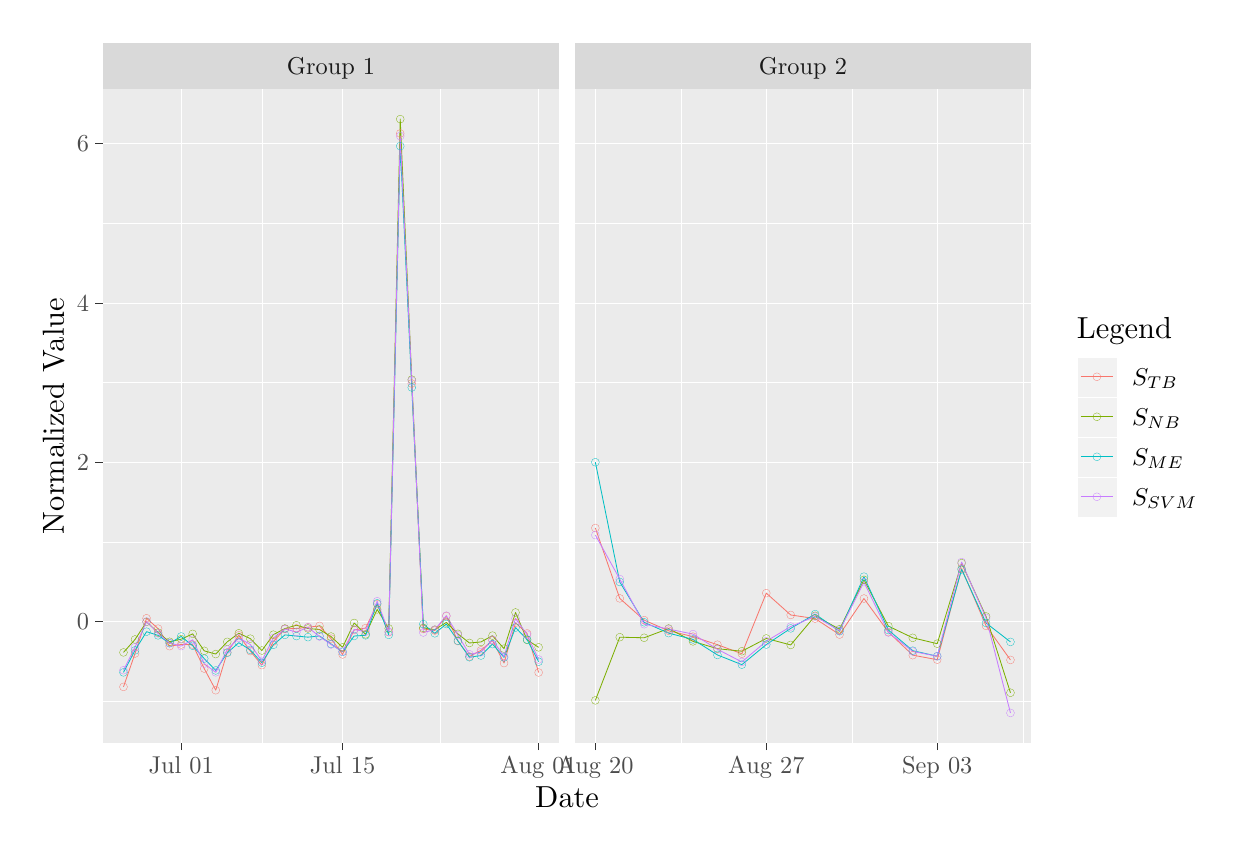
\begin{tikzpicture}[x=1pt,y=1pt]
\definecolor{fillColor}{RGB}{255,255,255}
\path[use as bounding box,fill=fillColor,fill opacity=0.00] (0,0) rectangle (433.62,289.08);
\begin{scope}
\path[clip] (  0.00,  0.00) rectangle (433.62,289.08);
\definecolor{drawColor}{RGB}{255,255,255}
\definecolor{fillColor}{RGB}{255,255,255}

\path[draw=drawColor,line width= 0.1pt,line join=round,line cap=round,fill=fillColor] (  0.00,  0.00) rectangle (433.62,289.08);
\end{scope}
\begin{scope}
\path[clip] ( 27.12, 30.73) rectangle (192.13,266.77);
\definecolor{fillColor}{gray}{0.92}

\path[fill=fillColor] ( 27.12, 30.73) rectangle (192.13,266.77);
\definecolor{drawColor}{RGB}{255,255,255}

\path[draw=drawColor,line width= 0.1pt,line join=round] ( 27.12, 45.81) --
	(192.13, 45.81);

\path[draw=drawColor,line width= 0.1pt,line join=round] ( 27.12,103.35) --
	(192.13,103.35);

\path[draw=drawColor,line width= 0.1pt,line join=round] ( 27.12,160.89) --
	(192.13,160.89);

\path[draw=drawColor,line width= 0.1pt,line join=round] ( 27.12,218.43) --
	(192.13,218.43);

\path[draw=drawColor,line width= 0.1pt,line join=round] ( 84.62, 30.73) --
	( 84.62,266.77);

\path[draw=drawColor,line width= 0.1pt,line join=round] (149.21, 30.73) --
	(149.21,266.77);

\path[draw=drawColor,line width= 0.1pt,line join=round] ( 27.12, 74.58) --
	(192.13, 74.58);

\path[draw=drawColor,line width= 0.1pt,line join=round] ( 27.12,132.12) --
	(192.13,132.12);

\path[draw=drawColor,line width= 0.1pt,line join=round] ( 27.12,189.66) --
	(192.13,189.66);

\path[draw=drawColor,line width= 0.1pt,line join=round] ( 27.12,247.20) --
	(192.13,247.20);

\path[draw=drawColor,line width= 0.1pt,line join=round] ( 55.46, 30.73) --
	( 55.46,266.77);

\path[draw=drawColor,line width= 0.1pt,line join=round] (113.79, 30.73) --
	(113.79,266.77);

\path[draw=drawColor,line width= 0.1pt,line join=round] (184.63, 30.73) --
	(184.63,266.77);
\definecolor{drawColor}{RGB}{248,118,109}

\path[draw=drawColor,line width= 0.3pt,line join=round] ( 34.62, 50.87) --
	( 38.79, 62.94) --
	( 42.96, 75.67) --
	( 47.12, 71.92) --
	( 51.29, 65.59) --
	( 55.46, 66.19) --
	( 59.62, 66.13) --
	( 63.79, 57.50) --
	( 67.96, 49.67) --
	( 72.12, 63.35) --
	( 76.29, 69.54) --
	( 80.46, 63.81) --
	( 84.62, 58.73) --
	( 88.79, 67.28) --
	( 92.96, 71.83) --
	( 97.12, 72.00) --
	(101.29, 72.43) --
	(105.46, 72.91) --
	(109.62, 68.30) --
	(113.79, 62.60) --
	(117.96, 71.44) --
	(122.12, 72.12) --
	(126.29, 80.78) --
	(130.46, 70.65) --
	(134.62,250.85) --
	(138.79,160.49) --
	(142.96, 71.80) --
	(147.12, 71.25) --
	(151.29, 76.47) --
	(155.46, 67.43) --
	(159.63, 61.83) --
	(163.79, 64.08) --
	(167.96, 67.68) --
	(172.13, 59.48) --
	(176.29, 74.04) --
	(180.46, 70.21) --
	(184.63, 56.07);
\definecolor{drawColor}{RGB}{124,174,0}

\path[draw=drawColor,line width= 0.3pt,line join=round] ( 34.62, 63.33) --
	( 38.79, 68.00) --
	( 42.96, 74.38) --
	( 47.12, 70.49) --
	( 51.29, 67.17) --
	( 55.46, 68.11) --
	( 59.62, 70.03) --
	( 63.79, 63.90) --
	( 67.96, 62.73) --
	( 72.12, 67.15) --
	( 76.29, 70.25) --
	( 80.46, 68.30) --
	( 84.62, 64.01) --
	( 88.79, 69.74) --
	( 92.96, 71.96) --
	( 97.12, 73.16) --
	(101.29, 71.97) --
	(105.46, 71.60) --
	(109.62, 69.06) --
	(113.79, 65.17) --
	(117.96, 73.97) --
	(122.12, 69.87) --
	(126.29, 78.87) --
	(130.46, 72.00) --
	(134.62,256.04) --
	(138.79,161.90) --
	(142.96, 72.20) --
	(147.12, 71.54) --
	(151.29, 74.18) --
	(155.46, 70.05) --
	(159.63, 66.74) --
	(163.79, 67.11) --
	(167.96, 69.39) --
	(172.13, 64.69) --
	(176.29, 77.76) --
	(180.46, 67.84) --
	(184.63, 65.17);
\definecolor{drawColor}{RGB}{0,191,196}

\path[draw=drawColor,line width= 0.3pt,line join=round] ( 34.62, 56.12) --
	( 38.79, 64.08) --
	( 42.96, 70.82) --
	( 47.12, 69.49) --
	( 51.29, 66.64) --
	( 55.46, 69.09) --
	( 59.62, 65.74) --
	( 63.79, 61.09) --
	( 67.96, 56.82) --
	( 72.12, 63.17) --
	( 76.29, 66.85) --
	( 80.46, 64.22) --
	( 84.62, 59.61) --
	( 88.79, 66.07) --
	( 92.96, 69.66) --
	( 97.12, 69.24) --
	(101.29, 68.84) --
	(105.46, 69.28) --
	(109.62, 66.38) --
	(113.79, 63.51) --
	(117.96, 69.26) --
	(122.12, 69.50) --
	(126.29, 81.08) --
	(130.46, 69.66) --
	(134.62,246.28) --
	(138.79,159.07) --
	(142.96, 73.54) --
	(147.12, 70.23) --
	(151.29, 73.59) --
	(155.46, 67.54) --
	(159.63, 61.59) --
	(163.79, 62.19) --
	(167.96, 66.35) --
	(172.13, 61.52) --
	(176.29, 72.30) --
	(180.46, 67.98) --
	(184.63, 59.98);
\definecolor{drawColor}{RGB}{199,124,255}

\path[draw=drawColor,line width= 0.3pt,line join=round] ( 34.62, 56.89) --
	( 38.79, 65.24) --
	( 42.96, 74.48) --
	( 47.12, 70.22) --
	( 51.29, 66.75) --
	( 55.46, 65.61) --
	( 59.62, 67.89) --
	( 63.79, 59.28) --
	( 67.96, 56.13) --
	( 72.12, 64.35) --
	( 76.29, 68.56) --
	( 80.46, 66.19) --
	( 84.62, 60.29) --
	( 88.79, 68.54) --
	( 92.96, 71.81) --
	( 97.12, 70.69) --
	(101.29, 72.36) --
	(105.46, 69.09) --
	(109.62, 66.19) --
	(113.79, 63.66) --
	(117.96, 71.61) --
	(122.12, 70.86) --
	(126.29, 81.82) --
	(130.46, 70.78) --
	(134.62,249.92) --
	(138.79,161.59) --
	(142.96, 70.53) --
	(147.12, 71.56) --
	(151.29, 76.61) --
	(155.46, 69.58) --
	(159.63, 62.65) --
	(163.79, 63.43) --
	(167.96, 67.88) --
	(172.13, 61.83) --
	(176.29, 75.60) --
	(180.46, 69.72) --
	(184.63, 60.77);
\definecolor{drawColor}{RGB}{248,118,109}

\path[draw=drawColor,line width= 0.1pt,line join=round,line cap=round] ( 34.62, 50.87) circle (  1.43);

\path[draw=drawColor,line width= 0.1pt,line join=round,line cap=round] ( 38.79, 62.94) circle (  1.43);

\path[draw=drawColor,line width= 0.1pt,line join=round,line cap=round] ( 42.96, 75.67) circle (  1.43);

\path[draw=drawColor,line width= 0.1pt,line join=round,line cap=round] ( 47.12, 71.92) circle (  1.43);

\path[draw=drawColor,line width= 0.1pt,line join=round,line cap=round] ( 51.29, 65.59) circle (  1.43);

\path[draw=drawColor,line width= 0.1pt,line join=round,line cap=round] ( 55.46, 66.19) circle (  1.43);

\path[draw=drawColor,line width= 0.1pt,line join=round,line cap=round] ( 59.62, 66.13) circle (  1.43);

\path[draw=drawColor,line width= 0.1pt,line join=round,line cap=round] ( 63.79, 57.50) circle (  1.43);

\path[draw=drawColor,line width= 0.1pt,line join=round,line cap=round] ( 67.96, 49.67) circle (  1.43);

\path[draw=drawColor,line width= 0.1pt,line join=round,line cap=round] ( 72.12, 63.35) circle (  1.43);

\path[draw=drawColor,line width= 0.1pt,line join=round,line cap=round] ( 76.29, 69.54) circle (  1.43);

\path[draw=drawColor,line width= 0.1pt,line join=round,line cap=round] ( 80.46, 63.81) circle (  1.43);

\path[draw=drawColor,line width= 0.1pt,line join=round,line cap=round] ( 84.62, 58.73) circle (  1.43);

\path[draw=drawColor,line width= 0.1pt,line join=round,line cap=round] ( 88.79, 67.28) circle (  1.43);

\path[draw=drawColor,line width= 0.1pt,line join=round,line cap=round] ( 92.96, 71.83) circle (  1.43);

\path[draw=drawColor,line width= 0.1pt,line join=round,line cap=round] ( 97.12, 72.00) circle (  1.43);

\path[draw=drawColor,line width= 0.1pt,line join=round,line cap=round] (101.29, 72.43) circle (  1.43);

\path[draw=drawColor,line width= 0.1pt,line join=round,line cap=round] (105.46, 72.91) circle (  1.43);

\path[draw=drawColor,line width= 0.1pt,line join=round,line cap=round] (109.62, 68.30) circle (  1.43);

\path[draw=drawColor,line width= 0.1pt,line join=round,line cap=round] (113.79, 62.60) circle (  1.43);

\path[draw=drawColor,line width= 0.1pt,line join=round,line cap=round] (117.96, 71.44) circle (  1.43);

\path[draw=drawColor,line width= 0.1pt,line join=round,line cap=round] (122.12, 72.12) circle (  1.43);

\path[draw=drawColor,line width= 0.1pt,line join=round,line cap=round] (126.29, 80.78) circle (  1.43);

\path[draw=drawColor,line width= 0.1pt,line join=round,line cap=round] (130.46, 70.65) circle (  1.43);

\path[draw=drawColor,line width= 0.1pt,line join=round,line cap=round] (134.62,250.85) circle (  1.43);

\path[draw=drawColor,line width= 0.1pt,line join=round,line cap=round] (138.79,160.49) circle (  1.43);

\path[draw=drawColor,line width= 0.1pt,line join=round,line cap=round] (142.96, 71.80) circle (  1.43);

\path[draw=drawColor,line width= 0.1pt,line join=round,line cap=round] (147.12, 71.25) circle (  1.43);

\path[draw=drawColor,line width= 0.1pt,line join=round,line cap=round] (151.29, 76.47) circle (  1.43);

\path[draw=drawColor,line width= 0.1pt,line join=round,line cap=round] (155.46, 67.43) circle (  1.43);

\path[draw=drawColor,line width= 0.1pt,line join=round,line cap=round] (159.63, 61.83) circle (  1.43);

\path[draw=drawColor,line width= 0.1pt,line join=round,line cap=round] (163.79, 64.08) circle (  1.43);

\path[draw=drawColor,line width= 0.1pt,line join=round,line cap=round] (167.96, 67.68) circle (  1.43);

\path[draw=drawColor,line width= 0.1pt,line join=round,line cap=round] (172.13, 59.48) circle (  1.43);

\path[draw=drawColor,line width= 0.1pt,line join=round,line cap=round] (176.29, 74.04) circle (  1.43);

\path[draw=drawColor,line width= 0.1pt,line join=round,line cap=round] (180.46, 70.21) circle (  1.43);

\path[draw=drawColor,line width= 0.1pt,line join=round,line cap=round] (184.63, 56.07) circle (  1.43);
\definecolor{drawColor}{RGB}{124,174,0}

\path[draw=drawColor,line width= 0.1pt,line join=round,line cap=round] ( 34.62, 63.33) circle (  1.43);

\path[draw=drawColor,line width= 0.1pt,line join=round,line cap=round] ( 38.79, 68.00) circle (  1.43);

\path[draw=drawColor,line width= 0.1pt,line join=round,line cap=round] ( 42.96, 74.38) circle (  1.43);

\path[draw=drawColor,line width= 0.1pt,line join=round,line cap=round] ( 47.12, 70.49) circle (  1.43);

\path[draw=drawColor,line width= 0.1pt,line join=round,line cap=round] ( 51.29, 67.17) circle (  1.43);

\path[draw=drawColor,line width= 0.1pt,line join=round,line cap=round] ( 55.46, 68.11) circle (  1.43);

\path[draw=drawColor,line width= 0.1pt,line join=round,line cap=round] ( 59.62, 70.03) circle (  1.43);

\path[draw=drawColor,line width= 0.1pt,line join=round,line cap=round] ( 63.79, 63.90) circle (  1.43);

\path[draw=drawColor,line width= 0.1pt,line join=round,line cap=round] ( 67.96, 62.73) circle (  1.43);

\path[draw=drawColor,line width= 0.1pt,line join=round,line cap=round] ( 72.12, 67.15) circle (  1.43);

\path[draw=drawColor,line width= 0.1pt,line join=round,line cap=round] ( 76.29, 70.25) circle (  1.43);

\path[draw=drawColor,line width= 0.1pt,line join=round,line cap=round] ( 80.46, 68.30) circle (  1.43);

\path[draw=drawColor,line width= 0.1pt,line join=round,line cap=round] ( 84.62, 64.01) circle (  1.43);

\path[draw=drawColor,line width= 0.1pt,line join=round,line cap=round] ( 88.79, 69.74) circle (  1.43);

\path[draw=drawColor,line width= 0.1pt,line join=round,line cap=round] ( 92.96, 71.96) circle (  1.43);

\path[draw=drawColor,line width= 0.1pt,line join=round,line cap=round] ( 97.12, 73.16) circle (  1.43);

\path[draw=drawColor,line width= 0.1pt,line join=round,line cap=round] (101.29, 71.97) circle (  1.43);

\path[draw=drawColor,line width= 0.1pt,line join=round,line cap=round] (105.46, 71.60) circle (  1.43);

\path[draw=drawColor,line width= 0.1pt,line join=round,line cap=round] (109.62, 69.06) circle (  1.43);

\path[draw=drawColor,line width= 0.1pt,line join=round,line cap=round] (113.79, 65.17) circle (  1.43);

\path[draw=drawColor,line width= 0.1pt,line join=round,line cap=round] (117.96, 73.97) circle (  1.43);

\path[draw=drawColor,line width= 0.1pt,line join=round,line cap=round] (122.12, 69.87) circle (  1.43);

\path[draw=drawColor,line width= 0.1pt,line join=round,line cap=round] (126.29, 78.87) circle (  1.43);

\path[draw=drawColor,line width= 0.1pt,line join=round,line cap=round] (130.46, 72.00) circle (  1.43);

\path[draw=drawColor,line width= 0.1pt,line join=round,line cap=round] (134.62,256.04) circle (  1.43);

\path[draw=drawColor,line width= 0.1pt,line join=round,line cap=round] (138.79,161.90) circle (  1.43);

\path[draw=drawColor,line width= 0.1pt,line join=round,line cap=round] (142.96, 72.20) circle (  1.43);

\path[draw=drawColor,line width= 0.1pt,line join=round,line cap=round] (147.12, 71.54) circle (  1.43);

\path[draw=drawColor,line width= 0.1pt,line join=round,line cap=round] (151.29, 74.18) circle (  1.43);

\path[draw=drawColor,line width= 0.1pt,line join=round,line cap=round] (155.46, 70.05) circle (  1.43);

\path[draw=drawColor,line width= 0.1pt,line join=round,line cap=round] (159.63, 66.74) circle (  1.43);

\path[draw=drawColor,line width= 0.1pt,line join=round,line cap=round] (163.79, 67.11) circle (  1.43);

\path[draw=drawColor,line width= 0.1pt,line join=round,line cap=round] (167.96, 69.39) circle (  1.43);

\path[draw=drawColor,line width= 0.1pt,line join=round,line cap=round] (172.13, 64.69) circle (  1.43);

\path[draw=drawColor,line width= 0.1pt,line join=round,line cap=round] (176.29, 77.76) circle (  1.43);

\path[draw=drawColor,line width= 0.1pt,line join=round,line cap=round] (180.46, 67.84) circle (  1.43);

\path[draw=drawColor,line width= 0.1pt,line join=round,line cap=round] (184.63, 65.17) circle (  1.43);
\definecolor{drawColor}{RGB}{0,191,196}

\path[draw=drawColor,line width= 0.1pt,line join=round,line cap=round] ( 34.62, 56.12) circle (  1.43);

\path[draw=drawColor,line width= 0.1pt,line join=round,line cap=round] ( 38.79, 64.08) circle (  1.43);

\path[draw=drawColor,line width= 0.1pt,line join=round,line cap=round] ( 42.96, 70.82) circle (  1.43);

\path[draw=drawColor,line width= 0.1pt,line join=round,line cap=round] ( 47.12, 69.49) circle (  1.43);

\path[draw=drawColor,line width= 0.1pt,line join=round,line cap=round] ( 51.29, 66.64) circle (  1.43);

\path[draw=drawColor,line width= 0.1pt,line join=round,line cap=round] ( 55.46, 69.09) circle (  1.43);

\path[draw=drawColor,line width= 0.1pt,line join=round,line cap=round] ( 59.62, 65.74) circle (  1.43);

\path[draw=drawColor,line width= 0.1pt,line join=round,line cap=round] ( 63.79, 61.09) circle (  1.43);

\path[draw=drawColor,line width= 0.1pt,line join=round,line cap=round] ( 67.96, 56.82) circle (  1.43);

\path[draw=drawColor,line width= 0.1pt,line join=round,line cap=round] ( 72.12, 63.17) circle (  1.43);

\path[draw=drawColor,line width= 0.1pt,line join=round,line cap=round] ( 76.29, 66.85) circle (  1.43);

\path[draw=drawColor,line width= 0.1pt,line join=round,line cap=round] ( 80.46, 64.22) circle (  1.43);

\path[draw=drawColor,line width= 0.1pt,line join=round,line cap=round] ( 84.62, 59.61) circle (  1.43);

\path[draw=drawColor,line width= 0.1pt,line join=round,line cap=round] ( 88.79, 66.07) circle (  1.43);

\path[draw=drawColor,line width= 0.1pt,line join=round,line cap=round] ( 92.96, 69.66) circle (  1.43);

\path[draw=drawColor,line width= 0.1pt,line join=round,line cap=round] ( 97.12, 69.24) circle (  1.43);

\path[draw=drawColor,line width= 0.1pt,line join=round,line cap=round] (101.29, 68.84) circle (  1.43);

\path[draw=drawColor,line width= 0.1pt,line join=round,line cap=round] (105.46, 69.28) circle (  1.43);

\path[draw=drawColor,line width= 0.1pt,line join=round,line cap=round] (109.62, 66.38) circle (  1.43);

\path[draw=drawColor,line width= 0.1pt,line join=round,line cap=round] (113.79, 63.51) circle (  1.43);

\path[draw=drawColor,line width= 0.1pt,line join=round,line cap=round] (117.96, 69.26) circle (  1.43);

\path[draw=drawColor,line width= 0.1pt,line join=round,line cap=round] (122.12, 69.50) circle (  1.43);

\path[draw=drawColor,line width= 0.1pt,line join=round,line cap=round] (126.29, 81.08) circle (  1.43);

\path[draw=drawColor,line width= 0.1pt,line join=round,line cap=round] (130.46, 69.66) circle (  1.43);

\path[draw=drawColor,line width= 0.1pt,line join=round,line cap=round] (134.62,246.28) circle (  1.43);

\path[draw=drawColor,line width= 0.1pt,line join=round,line cap=round] (138.79,159.07) circle (  1.43);

\path[draw=drawColor,line width= 0.1pt,line join=round,line cap=round] (142.96, 73.54) circle (  1.43);

\path[draw=drawColor,line width= 0.1pt,line join=round,line cap=round] (147.12, 70.23) circle (  1.43);

\path[draw=drawColor,line width= 0.1pt,line join=round,line cap=round] (151.29, 73.59) circle (  1.43);

\path[draw=drawColor,line width= 0.1pt,line join=round,line cap=round] (155.46, 67.54) circle (  1.43);

\path[draw=drawColor,line width= 0.1pt,line join=round,line cap=round] (159.63, 61.59) circle (  1.43);

\path[draw=drawColor,line width= 0.1pt,line join=round,line cap=round] (163.79, 62.19) circle (  1.43);

\path[draw=drawColor,line width= 0.1pt,line join=round,line cap=round] (167.96, 66.35) circle (  1.43);

\path[draw=drawColor,line width= 0.1pt,line join=round,line cap=round] (172.13, 61.52) circle (  1.43);

\path[draw=drawColor,line width= 0.1pt,line join=round,line cap=round] (176.29, 72.30) circle (  1.43);

\path[draw=drawColor,line width= 0.1pt,line join=round,line cap=round] (180.46, 67.98) circle (  1.43);

\path[draw=drawColor,line width= 0.1pt,line join=round,line cap=round] (184.63, 59.98) circle (  1.43);
\definecolor{drawColor}{RGB}{199,124,255}

\path[draw=drawColor,line width= 0.1pt,line join=round,line cap=round] ( 34.62, 56.89) circle (  1.43);

\path[draw=drawColor,line width= 0.1pt,line join=round,line cap=round] ( 38.79, 65.24) circle (  1.43);

\path[draw=drawColor,line width= 0.1pt,line join=round,line cap=round] ( 42.96, 74.48) circle (  1.43);

\path[draw=drawColor,line width= 0.1pt,line join=round,line cap=round] ( 47.12, 70.22) circle (  1.43);

\path[draw=drawColor,line width= 0.1pt,line join=round,line cap=round] ( 51.29, 66.75) circle (  1.43);

\path[draw=drawColor,line width= 0.1pt,line join=round,line cap=round] ( 55.46, 65.61) circle (  1.43);

\path[draw=drawColor,line width= 0.1pt,line join=round,line cap=round] ( 59.62, 67.89) circle (  1.43);

\path[draw=drawColor,line width= 0.1pt,line join=round,line cap=round] ( 63.79, 59.28) circle (  1.43);

\path[draw=drawColor,line width= 0.1pt,line join=round,line cap=round] ( 67.96, 56.13) circle (  1.43);

\path[draw=drawColor,line width= 0.1pt,line join=round,line cap=round] ( 72.12, 64.35) circle (  1.43);

\path[draw=drawColor,line width= 0.1pt,line join=round,line cap=round] ( 76.29, 68.56) circle (  1.43);

\path[draw=drawColor,line width= 0.1pt,line join=round,line cap=round] ( 80.46, 66.19) circle (  1.43);

\path[draw=drawColor,line width= 0.1pt,line join=round,line cap=round] ( 84.62, 60.29) circle (  1.43);

\path[draw=drawColor,line width= 0.1pt,line join=round,line cap=round] ( 88.79, 68.54) circle (  1.43);

\path[draw=drawColor,line width= 0.1pt,line join=round,line cap=round] ( 92.96, 71.81) circle (  1.43);

\path[draw=drawColor,line width= 0.1pt,line join=round,line cap=round] ( 97.12, 70.69) circle (  1.43);

\path[draw=drawColor,line width= 0.1pt,line join=round,line cap=round] (101.29, 72.36) circle (  1.43);

\path[draw=drawColor,line width= 0.1pt,line join=round,line cap=round] (105.46, 69.09) circle (  1.43);

\path[draw=drawColor,line width= 0.1pt,line join=round,line cap=round] (109.62, 66.19) circle (  1.43);

\path[draw=drawColor,line width= 0.1pt,line join=round,line cap=round] (113.79, 63.66) circle (  1.43);

\path[draw=drawColor,line width= 0.1pt,line join=round,line cap=round] (117.96, 71.61) circle (  1.43);

\path[draw=drawColor,line width= 0.1pt,line join=round,line cap=round] (122.12, 70.86) circle (  1.43);

\path[draw=drawColor,line width= 0.1pt,line join=round,line cap=round] (126.29, 81.82) circle (  1.43);

\path[draw=drawColor,line width= 0.1pt,line join=round,line cap=round] (130.46, 70.78) circle (  1.43);

\path[draw=drawColor,line width= 0.1pt,line join=round,line cap=round] (134.62,249.92) circle (  1.43);

\path[draw=drawColor,line width= 0.1pt,line join=round,line cap=round] (138.79,161.59) circle (  1.43);

\path[draw=drawColor,line width= 0.1pt,line join=round,line cap=round] (142.96, 70.53) circle (  1.43);

\path[draw=drawColor,line width= 0.1pt,line join=round,line cap=round] (147.12, 71.56) circle (  1.43);

\path[draw=drawColor,line width= 0.1pt,line join=round,line cap=round] (151.29, 76.61) circle (  1.43);

\path[draw=drawColor,line width= 0.1pt,line join=round,line cap=round] (155.46, 69.58) circle (  1.43);

\path[draw=drawColor,line width= 0.1pt,line join=round,line cap=round] (159.63, 62.65) circle (  1.43);

\path[draw=drawColor,line width= 0.1pt,line join=round,line cap=round] (163.79, 63.43) circle (  1.43);

\path[draw=drawColor,line width= 0.1pt,line join=round,line cap=round] (167.96, 67.88) circle (  1.43);

\path[draw=drawColor,line width= 0.1pt,line join=round,line cap=round] (172.13, 61.83) circle (  1.43);

\path[draw=drawColor,line width= 0.1pt,line join=round,line cap=round] (176.29, 75.60) circle (  1.43);

\path[draw=drawColor,line width= 0.1pt,line join=round,line cap=round] (180.46, 69.72) circle (  1.43);

\path[draw=drawColor,line width= 0.1pt,line join=round,line cap=round] (184.63, 60.77) circle (  1.43);
\end{scope}
\begin{scope}
\path[clip] (197.63, 30.73) rectangle (362.63,266.77);
\definecolor{fillColor}{gray}{0.92}

\path[fill=fillColor] (197.63, 30.73) rectangle (362.63,266.77);
\definecolor{drawColor}{RGB}{255,255,255}

\path[draw=drawColor,line width= 0.1pt,line join=round] (197.63, 45.81) --
	(362.63, 45.81);

\path[draw=drawColor,line width= 0.1pt,line join=round] (197.63,103.35) --
	(362.63,103.35);

\path[draw=drawColor,line width= 0.1pt,line join=round] (197.63,160.89) --
	(362.63,160.89);

\path[draw=drawColor,line width= 0.1pt,line join=round] (197.63,218.43) --
	(362.63,218.43);

\path[draw=drawColor,line width= 0.1pt,line join=round] (236.01, 30.73) --
	(236.01,266.77);

\path[draw=drawColor,line width= 0.1pt,line join=round] (297.78, 30.73) --
	(297.78,266.77);

\path[draw=drawColor,line width= 0.1pt,line join=round] (359.54, 30.73) --
	(359.54,266.77);

\path[draw=drawColor,line width= 0.1pt,line join=round] (197.63, 74.58) --
	(362.63, 74.58);

\path[draw=drawColor,line width= 0.1pt,line join=round] (197.63,132.12) --
	(362.63,132.12);

\path[draw=drawColor,line width= 0.1pt,line join=round] (197.63,189.66) --
	(362.63,189.66);

\path[draw=drawColor,line width= 0.1pt,line join=round] (197.63,247.20) --
	(362.63,247.20);

\path[draw=drawColor,line width= 0.1pt,line join=round] (205.13, 30.73) --
	(205.13,266.77);

\path[draw=drawColor,line width= 0.1pt,line join=round] (266.89, 30.73) --
	(266.89,266.77);

\path[draw=drawColor,line width= 0.1pt,line join=round] (328.66, 30.73) --
	(328.66,266.77);
\definecolor{drawColor}{RGB}{248,118,109}

\path[draw=drawColor,line width= 0.3pt,line join=round] (205.13,108.27) --
	(213.95, 82.85) --
	(222.77, 74.99) --
	(231.60, 71.16) --
	(240.42, 69.04) --
	(249.24, 66.12) --
	(258.07, 62.85) --
	(266.89, 84.75) --
	(275.72, 76.86) --
	(284.54, 75.56) --
	(293.36, 69.77) --
	(302.19, 82.80) --
	(311.01, 70.68) --
	(319.83, 62.33) --
	(328.66, 60.70) --
	(337.48, 93.62) --
	(346.31, 72.92) --
	(355.13, 60.61);
\definecolor{drawColor}{RGB}{124,174,0}

\path[draw=drawColor,line width= 0.3pt,line join=round] (205.13, 46.00) --
	(213.95, 68.83) --
	(222.77, 68.62) --
	(231.60, 71.96) --
	(240.42, 67.32) --
	(249.24, 64.67) --
	(258.07, 63.76) --
	(266.89, 68.37) --
	(275.72, 66.03) --
	(284.54, 76.55) --
	(293.36, 71.71) --
	(302.19, 89.56) --
	(311.01, 72.83) --
	(319.83, 68.60) --
	(328.66, 66.48) --
	(337.48, 95.59) --
	(346.31, 76.32) --
	(355.13, 48.76);
\definecolor{drawColor}{RGB}{0,191,196}

\path[draw=drawColor,line width= 0.3pt,line join=round] (205.13,132.05) --
	(213.95, 88.78) --
	(222.77, 74.21) --
	(231.60, 70.30) --
	(240.42, 68.01) --
	(249.24, 62.42) --
	(258.07, 58.90) --
	(266.89, 66.17) --
	(275.72, 72.01) --
	(284.54, 77.17) --
	(293.36, 70.99) --
	(302.19, 90.70) --
	(311.01, 71.41) --
	(319.83, 63.96) --
	(328.66, 61.96) --
	(337.48, 93.29) --
	(346.31, 73.96) --
	(355.13, 67.12);
\definecolor{drawColor}{RGB}{199,124,255}

\path[draw=drawColor,line width= 0.3pt,line join=round] (205.13,105.73) --
	(213.95, 89.83) --
	(222.77, 73.53) --
	(231.60, 71.77) --
	(240.42, 69.94) --
	(249.24, 64.47) --
	(258.07, 59.89) --
	(266.89, 67.36) --
	(275.72, 72.67) --
	(284.54, 76.33) --
	(293.36, 71.20) --
	(302.19, 88.72) --
	(311.01, 70.54) --
	(319.83, 63.69) --
	(328.66, 61.94) --
	(337.48, 95.96) --
	(346.31, 75.81) --
	(355.13, 41.46);
\definecolor{drawColor}{RGB}{248,118,109}

\path[draw=drawColor,line width= 0.1pt,line join=round,line cap=round] (205.13,108.27) circle (  1.43);

\path[draw=drawColor,line width= 0.1pt,line join=round,line cap=round] (213.95, 82.85) circle (  1.43);

\path[draw=drawColor,line width= 0.1pt,line join=round,line cap=round] (222.77, 74.99) circle (  1.43);

\path[draw=drawColor,line width= 0.1pt,line join=round,line cap=round] (231.60, 71.16) circle (  1.43);

\path[draw=drawColor,line width= 0.1pt,line join=round,line cap=round] (240.42, 69.04) circle (  1.43);

\path[draw=drawColor,line width= 0.1pt,line join=round,line cap=round] (249.24, 66.12) circle (  1.43);

\path[draw=drawColor,line width= 0.1pt,line join=round,line cap=round] (258.07, 62.85) circle (  1.43);

\path[draw=drawColor,line width= 0.1pt,line join=round,line cap=round] (266.89, 84.75) circle (  1.43);

\path[draw=drawColor,line width= 0.1pt,line join=round,line cap=round] (275.72, 76.86) circle (  1.43);

\path[draw=drawColor,line width= 0.1pt,line join=round,line cap=round] (284.54, 75.56) circle (  1.43);

\path[draw=drawColor,line width= 0.1pt,line join=round,line cap=round] (293.36, 69.77) circle (  1.43);

\path[draw=drawColor,line width= 0.1pt,line join=round,line cap=round] (302.19, 82.80) circle (  1.43);

\path[draw=drawColor,line width= 0.1pt,line join=round,line cap=round] (311.01, 70.68) circle (  1.43);

\path[draw=drawColor,line width= 0.1pt,line join=round,line cap=round] (319.83, 62.33) circle (  1.43);

\path[draw=drawColor,line width= 0.1pt,line join=round,line cap=round] (328.66, 60.70) circle (  1.43);

\path[draw=drawColor,line width= 0.1pt,line join=round,line cap=round] (337.48, 93.62) circle (  1.43);

\path[draw=drawColor,line width= 0.1pt,line join=round,line cap=round] (346.31, 72.92) circle (  1.43);

\path[draw=drawColor,line width= 0.1pt,line join=round,line cap=round] (355.13, 60.61) circle (  1.43);
\definecolor{drawColor}{RGB}{124,174,0}

\path[draw=drawColor,line width= 0.1pt,line join=round,line cap=round] (205.13, 46.00) circle (  1.43);

\path[draw=drawColor,line width= 0.1pt,line join=round,line cap=round] (213.95, 68.83) circle (  1.43);

\path[draw=drawColor,line width= 0.1pt,line join=round,line cap=round] (222.77, 68.62) circle (  1.43);

\path[draw=drawColor,line width= 0.1pt,line join=round,line cap=round] (231.60, 71.96) circle (  1.43);

\path[draw=drawColor,line width= 0.1pt,line join=round,line cap=round] (240.42, 67.32) circle (  1.43);

\path[draw=drawColor,line width= 0.1pt,line join=round,line cap=round] (249.24, 64.67) circle (  1.43);

\path[draw=drawColor,line width= 0.1pt,line join=round,line cap=round] (258.07, 63.76) circle (  1.43);

\path[draw=drawColor,line width= 0.1pt,line join=round,line cap=round] (266.89, 68.37) circle (  1.43);

\path[draw=drawColor,line width= 0.1pt,line join=round,line cap=round] (275.72, 66.03) circle (  1.43);

\path[draw=drawColor,line width= 0.1pt,line join=round,line cap=round] (284.54, 76.55) circle (  1.43);

\path[draw=drawColor,line width= 0.1pt,line join=round,line cap=round] (293.36, 71.71) circle (  1.43);

\path[draw=drawColor,line width= 0.1pt,line join=round,line cap=round] (302.19, 89.56) circle (  1.43);

\path[draw=drawColor,line width= 0.1pt,line join=round,line cap=round] (311.01, 72.83) circle (  1.43);

\path[draw=drawColor,line width= 0.1pt,line join=round,line cap=round] (319.83, 68.60) circle (  1.43);

\path[draw=drawColor,line width= 0.1pt,line join=round,line cap=round] (328.66, 66.48) circle (  1.43);

\path[draw=drawColor,line width= 0.1pt,line join=round,line cap=round] (337.48, 95.59) circle (  1.43);

\path[draw=drawColor,line width= 0.1pt,line join=round,line cap=round] (346.31, 76.32) circle (  1.43);

\path[draw=drawColor,line width= 0.1pt,line join=round,line cap=round] (355.13, 48.76) circle (  1.43);
\definecolor{drawColor}{RGB}{0,191,196}

\path[draw=drawColor,line width= 0.1pt,line join=round,line cap=round] (205.13,132.05) circle (  1.43);

\path[draw=drawColor,line width= 0.1pt,line join=round,line cap=round] (213.95, 88.78) circle (  1.43);

\path[draw=drawColor,line width= 0.1pt,line join=round,line cap=round] (222.77, 74.21) circle (  1.43);

\path[draw=drawColor,line width= 0.1pt,line join=round,line cap=round] (231.60, 70.30) circle (  1.43);

\path[draw=drawColor,line width= 0.1pt,line join=round,line cap=round] (240.42, 68.01) circle (  1.43);

\path[draw=drawColor,line width= 0.1pt,line join=round,line cap=round] (249.24, 62.42) circle (  1.43);

\path[draw=drawColor,line width= 0.1pt,line join=round,line cap=round] (258.07, 58.90) circle (  1.43);

\path[draw=drawColor,line width= 0.1pt,line join=round,line cap=round] (266.89, 66.17) circle (  1.43);

\path[draw=drawColor,line width= 0.1pt,line join=round,line cap=round] (275.72, 72.01) circle (  1.43);

\path[draw=drawColor,line width= 0.1pt,line join=round,line cap=round] (284.54, 77.17) circle (  1.43);

\path[draw=drawColor,line width= 0.1pt,line join=round,line cap=round] (293.36, 70.99) circle (  1.43);

\path[draw=drawColor,line width= 0.1pt,line join=round,line cap=round] (302.19, 90.70) circle (  1.43);

\path[draw=drawColor,line width= 0.1pt,line join=round,line cap=round] (311.01, 71.41) circle (  1.43);

\path[draw=drawColor,line width= 0.1pt,line join=round,line cap=round] (319.83, 63.96) circle (  1.43);

\path[draw=drawColor,line width= 0.1pt,line join=round,line cap=round] (328.66, 61.96) circle (  1.43);

\path[draw=drawColor,line width= 0.1pt,line join=round,line cap=round] (337.48, 93.29) circle (  1.43);

\path[draw=drawColor,line width= 0.1pt,line join=round,line cap=round] (346.31, 73.96) circle (  1.43);

\path[draw=drawColor,line width= 0.1pt,line join=round,line cap=round] (355.13, 67.12) circle (  1.43);
\definecolor{drawColor}{RGB}{199,124,255}

\path[draw=drawColor,line width= 0.1pt,line join=round,line cap=round] (205.13,105.73) circle (  1.43);

\path[draw=drawColor,line width= 0.1pt,line join=round,line cap=round] (213.95, 89.83) circle (  1.43);

\path[draw=drawColor,line width= 0.1pt,line join=round,line cap=round] (222.77, 73.53) circle (  1.43);

\path[draw=drawColor,line width= 0.1pt,line join=round,line cap=round] (231.60, 71.77) circle (  1.43);

\path[draw=drawColor,line width= 0.1pt,line join=round,line cap=round] (240.42, 69.94) circle (  1.43);

\path[draw=drawColor,line width= 0.1pt,line join=round,line cap=round] (249.24, 64.47) circle (  1.43);

\path[draw=drawColor,line width= 0.1pt,line join=round,line cap=round] (258.07, 59.89) circle (  1.43);

\path[draw=drawColor,line width= 0.1pt,line join=round,line cap=round] (266.89, 67.36) circle (  1.43);

\path[draw=drawColor,line width= 0.1pt,line join=round,line cap=round] (275.72, 72.67) circle (  1.43);

\path[draw=drawColor,line width= 0.1pt,line join=round,line cap=round] (284.54, 76.33) circle (  1.43);

\path[draw=drawColor,line width= 0.1pt,line join=round,line cap=round] (293.36, 71.20) circle (  1.43);

\path[draw=drawColor,line width= 0.1pt,line join=round,line cap=round] (302.19, 88.72) circle (  1.43);

\path[draw=drawColor,line width= 0.1pt,line join=round,line cap=round] (311.01, 70.54) circle (  1.43);

\path[draw=drawColor,line width= 0.1pt,line join=round,line cap=round] (319.83, 63.69) circle (  1.43);

\path[draw=drawColor,line width= 0.1pt,line join=round,line cap=round] (328.66, 61.94) circle (  1.43);

\path[draw=drawColor,line width= 0.1pt,line join=round,line cap=round] (337.48, 95.96) circle (  1.43);

\path[draw=drawColor,line width= 0.1pt,line join=round,line cap=round] (346.31, 75.81) circle (  1.43);

\path[draw=drawColor,line width= 0.1pt,line join=round,line cap=round] (355.13, 41.46) circle (  1.43);
\end{scope}
\begin{scope}
\path[clip] ( 27.12,266.77) rectangle (192.13,283.58);
\definecolor{fillColor}{gray}{0.85}

\path[fill=fillColor] ( 27.12,266.77) rectangle (192.13,283.58);
\definecolor{drawColor}{gray}{0.10}

\node[text=drawColor,anchor=base,inner sep=0pt, outer sep=0pt, scale=  0.88] at (109.62,272.15) {Group 1};
\end{scope}
\begin{scope}
\path[clip] (197.63,266.77) rectangle (362.63,283.58);
\definecolor{fillColor}{gray}{0.85}

\path[fill=fillColor] (197.63,266.77) rectangle (362.63,283.58);
\definecolor{drawColor}{gray}{0.10}

\node[text=drawColor,anchor=base,inner sep=0pt, outer sep=0pt, scale=  0.88] at (280.13,272.15) {Group 2};
\end{scope}
\begin{scope}
\path[clip] (  0.00,  0.00) rectangle (433.62,289.08);
\definecolor{drawColor}{gray}{0.20}

\path[draw=drawColor,line width= 0.1pt,line join=round] ( 55.46, 27.98) --
	( 55.46, 30.73);

\path[draw=drawColor,line width= 0.1pt,line join=round] (113.79, 27.98) --
	(113.79, 30.73);

\path[draw=drawColor,line width= 0.1pt,line join=round] (184.63, 27.98) --
	(184.63, 30.73);
\end{scope}
\begin{scope}
\path[clip] (  0.00,  0.00) rectangle (433.62,289.08);
\definecolor{drawColor}{gray}{0.30}

\node[text=drawColor,anchor=base,inner sep=0pt, outer sep=0pt, scale=  0.88] at ( 55.46, 19.72) {Jul 01};

\node[text=drawColor,anchor=base,inner sep=0pt, outer sep=0pt, scale=  0.88] at (113.79, 19.72) {Jul 15};

\node[text=drawColor,anchor=base,inner sep=0pt, outer sep=0pt, scale=  0.88] at (184.63, 19.72) {Aug 01};
\end{scope}
\begin{scope}
\path[clip] (  0.00,  0.00) rectangle (433.62,289.08);
\definecolor{drawColor}{gray}{0.20}

\path[draw=drawColor,line width= 0.1pt,line join=round] (205.13, 27.98) --
	(205.13, 30.73);

\path[draw=drawColor,line width= 0.1pt,line join=round] (266.89, 27.98) --
	(266.89, 30.73);

\path[draw=drawColor,line width= 0.1pt,line join=round] (328.66, 27.98) --
	(328.66, 30.73);
\end{scope}
\begin{scope}
\path[clip] (  0.00,  0.00) rectangle (433.62,289.08);
\definecolor{drawColor}{gray}{0.30}

\node[text=drawColor,anchor=base,inner sep=0pt, outer sep=0pt, scale=  0.88] at (205.13, 19.72) {Aug 20};

\node[text=drawColor,anchor=base,inner sep=0pt, outer sep=0pt, scale=  0.88] at (266.89, 19.72) {Aug 27};

\node[text=drawColor,anchor=base,inner sep=0pt, outer sep=0pt, scale=  0.88] at (328.66, 19.72) {Sep 03};
\end{scope}
\begin{scope}
\path[clip] (  0.00,  0.00) rectangle (433.62,289.08);
\definecolor{drawColor}{gray}{0.30}

\node[text=drawColor,anchor=base east,inner sep=0pt, outer sep=0pt, scale=  0.88] at ( 22.17, 71.55) {0};

\node[text=drawColor,anchor=base east,inner sep=0pt, outer sep=0pt, scale=  0.88] at ( 22.17,129.09) {2};

\node[text=drawColor,anchor=base east,inner sep=0pt, outer sep=0pt, scale=  0.88] at ( 22.17,186.63) {4};

\node[text=drawColor,anchor=base east,inner sep=0pt, outer sep=0pt, scale=  0.88] at ( 22.17,244.17) {6};
\end{scope}
\begin{scope}
\path[clip] (  0.00,  0.00) rectangle (433.62,289.08);
\definecolor{drawColor}{gray}{0.20}

\path[draw=drawColor,line width= 0.1pt,line join=round] ( 24.37, 74.58) --
	( 27.12, 74.58);

\path[draw=drawColor,line width= 0.1pt,line join=round] ( 24.37,132.12) --
	( 27.12,132.12);

\path[draw=drawColor,line width= 0.1pt,line join=round] ( 24.37,189.66) --
	( 27.12,189.66);

\path[draw=drawColor,line width= 0.1pt,line join=round] ( 24.37,247.20) --
	( 27.12,247.20);
\end{scope}
\begin{scope}
\path[clip] (  0.00,  0.00) rectangle (433.62,289.08);
\definecolor{drawColor}{RGB}{0,0,0}

\node[text=drawColor,anchor=base,inner sep=0pt, outer sep=0pt, scale=  1.10] at (194.88,  7.44) {Date};
\end{scope}
\begin{scope}
\path[clip] (  0.00,  0.00) rectangle (433.62,289.08);
\definecolor{drawColor}{RGB}{0,0,0}

\node[text=drawColor,rotate= 90.00,anchor=base,inner sep=0pt, outer sep=0pt, scale=  1.10] at ( 13.08,148.75) {Normalized Value};
\end{scope}
\begin{scope}
\path[clip] (  0.00,  0.00) rectangle (433.62,289.08);
\definecolor{fillColor}{RGB}{255,255,255}

\path[fill=fillColor] (373.63,106.83) rectangle (428.12,190.67);
\end{scope}
\begin{scope}
\path[clip] (  0.00,  0.00) rectangle (433.62,289.08);
\definecolor{drawColor}{RGB}{0,0,0}

\node[text=drawColor,anchor=base west,inner sep=0pt, outer sep=0pt, scale=  1.10] at (379.13,176.62) {Legend};
\end{scope}
\begin{scope}
\path[clip] (  0.00,  0.00) rectangle (433.62,289.08);
\definecolor{drawColor}{RGB}{255,255,255}
\definecolor{fillColor}{gray}{0.95}

\path[draw=drawColor,line width= 0.1pt,line join=round,line cap=round,fill=fillColor] (379.13,155.69) rectangle (393.58,170.15);
\end{scope}
\begin{scope}
\path[clip] (  0.00,  0.00) rectangle (433.62,289.08);
\definecolor{drawColor}{RGB}{248,118,109}

\path[draw=drawColor,line width= 0.3pt,line join=round] (380.57,162.92) -- (392.14,162.92);
\end{scope}
\begin{scope}
\path[clip] (  0.00,  0.00) rectangle (433.62,289.08);
\definecolor{drawColor}{RGB}{248,118,109}

\path[draw=drawColor,line width= 0.1pt,line join=round,line cap=round] (386.36,162.92) circle (  1.43);
\end{scope}
\begin{scope}
\path[clip] (  0.00,  0.00) rectangle (433.62,289.08);
\definecolor{drawColor}{RGB}{255,255,255}
\definecolor{fillColor}{gray}{0.95}

\path[draw=drawColor,line width= 0.1pt,line join=round,line cap=round,fill=fillColor] (379.13,141.24) rectangle (393.58,155.69);
\end{scope}
\begin{scope}
\path[clip] (  0.00,  0.00) rectangle (433.62,289.08);
\definecolor{drawColor}{RGB}{124,174,0}

\path[draw=drawColor,line width= 0.3pt,line join=round] (380.57,148.47) -- (392.14,148.47);
\end{scope}
\begin{scope}
\path[clip] (  0.00,  0.00) rectangle (433.62,289.08);
\definecolor{drawColor}{RGB}{124,174,0}

\path[draw=drawColor,line width= 0.1pt,line join=round,line cap=round] (386.36,148.47) circle (  1.43);
\end{scope}
\begin{scope}
\path[clip] (  0.00,  0.00) rectangle (433.62,289.08);
\definecolor{drawColor}{RGB}{255,255,255}
\definecolor{fillColor}{gray}{0.95}

\path[draw=drawColor,line width= 0.1pt,line join=round,line cap=round,fill=fillColor] (379.13,126.79) rectangle (393.58,141.24);
\end{scope}
\begin{scope}
\path[clip] (  0.00,  0.00) rectangle (433.62,289.08);
\definecolor{drawColor}{RGB}{0,191,196}

\path[draw=drawColor,line width= 0.3pt,line join=round] (380.57,134.01) -- (392.14,134.01);
\end{scope}
\begin{scope}
\path[clip] (  0.00,  0.00) rectangle (433.62,289.08);
\definecolor{drawColor}{RGB}{0,191,196}

\path[draw=drawColor,line width= 0.1pt,line join=round,line cap=round] (386.36,134.01) circle (  1.43);
\end{scope}
\begin{scope}
\path[clip] (  0.00,  0.00) rectangle (433.62,289.08);
\definecolor{drawColor}{RGB}{255,255,255}
\definecolor{fillColor}{gray}{0.95}

\path[draw=drawColor,line width= 0.1pt,line join=round,line cap=round,fill=fillColor] (379.13,112.33) rectangle (393.58,126.79);
\end{scope}
\begin{scope}
\path[clip] (  0.00,  0.00) rectangle (433.62,289.08);
\definecolor{drawColor}{RGB}{199,124,255}

\path[draw=drawColor,line width= 0.3pt,line join=round] (380.57,119.56) -- (392.14,119.56);
\end{scope}
\begin{scope}
\path[clip] (  0.00,  0.00) rectangle (433.62,289.08);
\definecolor{drawColor}{RGB}{199,124,255}

\path[draw=drawColor,line width= 0.1pt,line join=round,line cap=round] (386.36,119.56) circle (  1.43);
\end{scope}
\begin{scope}
\path[clip] (  0.00,  0.00) rectangle (433.62,289.08);
\definecolor{drawColor}{RGB}{0,0,0}

\node[text=drawColor,anchor=base west,inner sep=0pt, outer sep=0pt, scale=  0.88] at (399.08,159.89) {$S_{TB}$};
\end{scope}
\begin{scope}
\path[clip] (  0.00,  0.00) rectangle (433.62,289.08);
\definecolor{drawColor}{RGB}{0,0,0}

\node[text=drawColor,anchor=base west,inner sep=0pt, outer sep=0pt, scale=  0.88] at (399.08,145.44) {$S_{NB}$};
\end{scope}
\begin{scope}
\path[clip] (  0.00,  0.00) rectangle (433.62,289.08);
\definecolor{drawColor}{RGB}{0,0,0}

\node[text=drawColor,anchor=base west,inner sep=0pt, outer sep=0pt, scale=  0.88] at (399.08,130.98) {$S_{ME}$};
\end{scope}
\begin{scope}
\path[clip] (  0.00,  0.00) rectangle (433.62,289.08);
\definecolor{drawColor}{RGB}{0,0,0}

\node[text=drawColor,anchor=base west,inner sep=0pt, outer sep=0pt, scale=  0.88] at (399.08,116.53) {$S_{SVM}$};
\end{scope}
\end{tikzpicture}

    \caption{\sentimentsCaption{\gm}}
    \label{fig:analysis-sentiments-gm}
\end{figure} 

\subsection{\hyundai}
\label{ss:analysis-sentiments-hyundai}

\begin{figure}[hbt]
    \centering
    % Created by tikzDevice version 0.12 on 2019-04-11 07:15:59
% !TEX encoding = UTF-8 Unicode
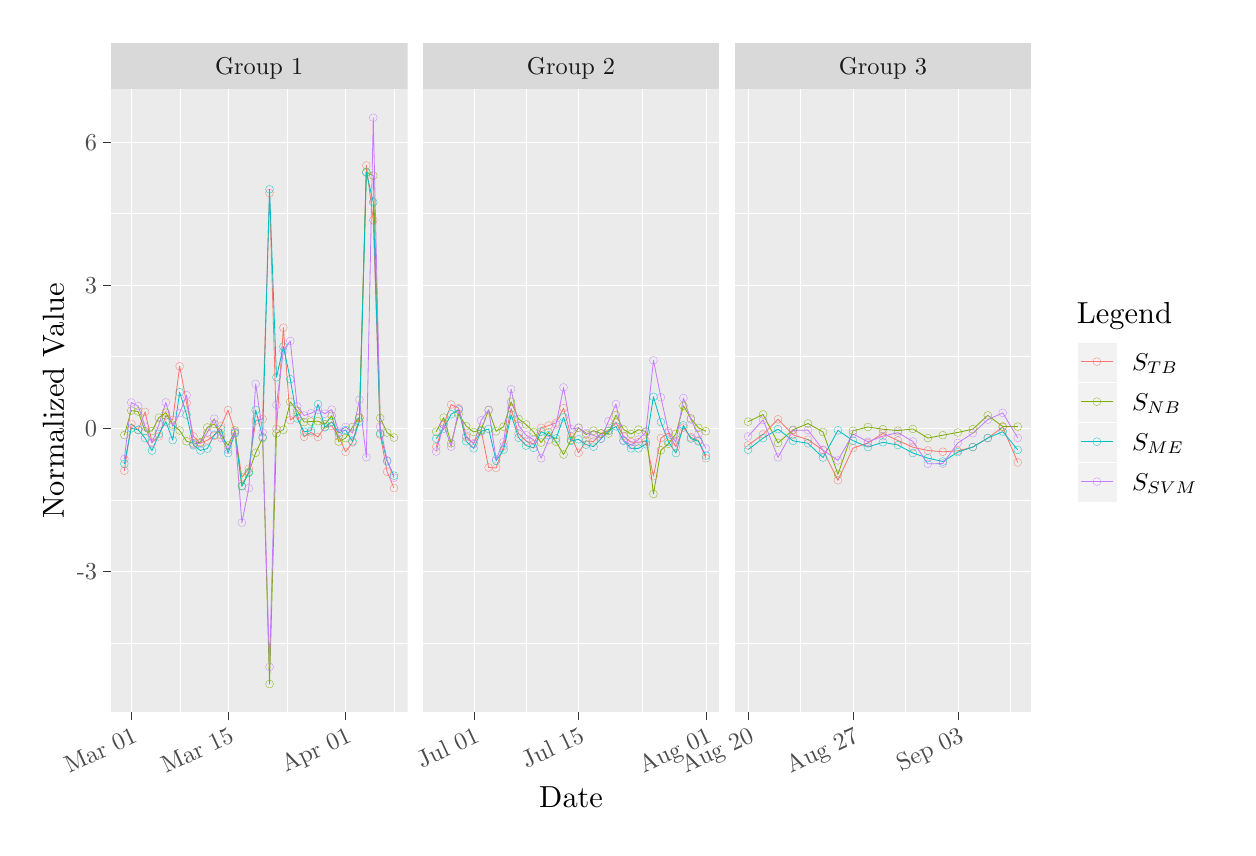
\begin{tikzpicture}[x=1pt,y=1pt]
\definecolor{fillColor}{RGB}{255,255,255}
\path[use as bounding box,fill=fillColor,fill opacity=0.00] (0,0) rectangle (433.62,289.08);
\begin{scope}
\path[clip] (  0.00,  0.00) rectangle (433.62,289.08);
\definecolor{drawColor}{RGB}{255,255,255}
\definecolor{fillColor}{RGB}{255,255,255}

\path[draw=drawColor,line width= 0.1pt,line join=round,line cap=round,fill=fillColor] (  0.00,  0.00) rectangle (433.62,289.08);
\end{scope}
\begin{scope}
\path[clip] ( 30.06, 41.66) rectangle (137.25,266.77);
\definecolor{fillColor}{gray}{0.92}

\path[fill=fillColor] ( 30.06, 41.66) rectangle (137.25,266.77);
\definecolor{drawColor}{RGB}{255,255,255}

\path[draw=drawColor,line width= 0.1pt,line join=round] ( 30.06, 66.66) --
	(137.25, 66.66);

\path[draw=drawColor,line width= 0.1pt,line join=round] ( 30.06,118.44) --
	(137.25,118.44);

\path[draw=drawColor,line width= 0.1pt,line join=round] ( 30.06,170.22) --
	(137.25,170.22);

\path[draw=drawColor,line width= 0.1pt,line join=round] ( 30.06,222.00) --
	(137.25,222.00);

\path[draw=drawColor,line width= 0.1pt,line join=round] ( 54.92, 41.66) --
	( 54.92,266.77);

\path[draw=drawColor,line width= 0.1pt,line join=round] ( 93.65, 41.66) --
	( 93.65,266.77);

\path[draw=drawColor,line width= 0.1pt,line join=round] (132.37, 41.66) --
	(132.37,266.77);

\path[draw=drawColor,line width= 0.1pt,line join=round] ( 30.06, 92.55) --
	(137.25, 92.55);

\path[draw=drawColor,line width= 0.1pt,line join=round] ( 30.06,144.33) --
	(137.25,144.33);

\path[draw=drawColor,line width= 0.1pt,line join=round] ( 30.06,196.11) --
	(137.25,196.11);

\path[draw=drawColor,line width= 0.1pt,line join=round] ( 30.06,247.89) --
	(137.25,247.89);

\path[draw=drawColor,line width= 0.1pt,line join=round] ( 37.43, 41.66) --
	( 37.43,266.77);

\path[draw=drawColor,line width= 0.1pt,line join=round] ( 72.41, 41.66) --
	( 72.41,266.77);

\path[draw=drawColor,line width= 0.1pt,line join=round] (114.88, 41.66) --
	(114.88,266.77);
\definecolor{drawColor}{RGB}{248,118,109}

\path[draw=drawColor,line width= 0.3pt,line join=round] ( 34.93,128.99) --
	( 37.43,145.95) --
	( 39.93,143.72) --
	( 42.42,150.25) --
	( 44.92,139.23) --
	( 47.42,141.40) --
	( 49.92,148.95) --
	( 52.42,147.35) --
	( 54.92,166.72) --
	( 57.42,153.41) --
	( 59.91,141.41) --
	( 62.41,138.89) --
	( 64.91,139.99) --
	( 67.41,141.63) --
	( 69.91,145.17) --
	( 72.41,150.86) --
	( 74.91,142.87) --
	( 77.40,126.61) --
	( 79.90,129.70) --
	( 82.40,147.11) --
	( 84.90,147.66) --
	( 87.40,229.33) --
	( 89.90,144.08) --
	( 92.40,180.64) --
	( 94.89,147.26) --
	( 97.39,149.35) --
	( 99.89,141.24) --
	(102.39,142.84) --
	(104.89,141.16) --
	(107.39,144.82) --
	(109.89,145.16) --
	(112.39,141.45) --
	(114.88,135.80) --
	(117.38,139.23) --
	(119.88,148.00) --
	(122.38,239.30) --
	(124.88,219.48) --
	(127.38,142.05) --
	(129.88,128.61) --
	(132.37,122.72);
\definecolor{drawColor}{RGB}{124,174,0}

\path[draw=drawColor,line width= 0.3pt,line join=round] ( 34.93,141.85) --
	( 37.43,150.71) --
	( 39.93,150.38) --
	( 42.42,143.29) --
	( 44.92,143.32) --
	( 47.42,148.17) --
	( 49.92,149.94) --
	( 52.42,145.59) --
	( 54.92,143.52) --
	( 57.42,139.62) --
	( 59.91,138.84) --
	( 62.41,139.29) --
	( 64.91,144.62) --
	( 67.41,145.92) --
	( 69.91,141.86) --
	( 72.41,138.14) --
	( 74.91,143.55) --
	( 77.40,123.49) --
	( 79.90,128.51) --
	( 82.40,135.47) --
	( 84.90,140.78) --
	( 87.40, 51.89) --
	( 89.90,142.50) --
	( 92.40,143.78) --
	( 94.89,153.86) --
	( 97.39,150.64) --
	( 99.89,146.56) --
	(102.39,146.77) --
	(104.89,146.90) --
	(107.39,145.75) --
	(109.89,148.89) --
	(112.39,139.52) --
	(114.88,140.78) --
	(117.38,144.78) --
	(119.88,148.21) --
	(122.38,236.97) --
	(124.88,235.60) --
	(127.38,148.03) --
	(129.88,142.76) --
	(132.37,140.96);
\definecolor{drawColor}{RGB}{0,191,196}

\path[draw=drawColor,line width= 0.3pt,line join=round] ( 34.93,131.50) --
	( 37.43,144.30) --
	( 39.93,143.78) --
	( 42.42,140.77) --
	( 44.92,136.22) --
	( 47.42,142.27) --
	( 49.92,146.72) --
	( 52.42,140.03) --
	( 54.92,157.34) --
	( 57.42,149.23) --
	( 59.91,138.18) --
	( 62.41,136.31) --
	( 64.91,136.97) --
	( 67.41,141.96) --
	( 69.91,144.05) --
	( 72.41,135.35) --
	( 74.91,142.50) --
	( 77.40,123.37) --
	( 79.90,128.25) --
	( 82.40,150.93) --
	( 84.90,141.13) --
	( 87.40,230.66) --
	( 89.90,162.77) --
	( 92.40,173.82) --
	( 94.89,162.06) --
	( 97.39,147.89) --
	( 99.89,143.05) --
	(102.39,143.42) --
	(104.89,153.04) --
	(107.39,144.70) --
	(109.89,146.63) --
	(112.39,142.61) --
	(114.88,143.71) --
	(117.38,139.58) --
	(119.88,146.75) --
	(122.38,236.72) --
	(124.88,226.00) --
	(127.38,142.45) --
	(129.88,132.40) --
	(132.37,127.21);
\definecolor{drawColor}{RGB}{199,124,255}

\path[draw=drawColor,line width= 0.3pt,line join=round] ( 34.93,133.25) --
	( 37.43,153.61) --
	( 39.93,152.32) --
	( 42.42,144.90) --
	( 44.92,138.99) --
	( 47.42,145.68) --
	( 49.92,153.68) --
	( 52.42,145.00) --
	( 54.92,149.81) --
	( 57.42,156.28) --
	( 59.91,138.55) --
	( 62.41,138.92) --
	( 64.91,142.83) --
	( 67.41,147.78) --
	( 69.91,140.88) --
	( 72.41,136.60) --
	( 74.91,142.99) --
	( 77.40,110.22) --
	( 79.90,122.66) --
	( 82.40,160.36) --
	( 84.90,142.82) --
	( 87.40, 58.08) --
	( 89.90,152.80) --
	( 92.40,172.37) --
	( 94.89,175.86) --
	( 97.39,152.20) --
	( 99.89,148.95) --
	(102.39,149.73) --
	(104.89,151.03) --
	(107.39,149.58) --
	(109.89,151.07) --
	(112.39,143.10) --
	(114.88,144.82) --
	(117.38,142.61) --
	(119.88,154.62) --
	(122.38,133.86) --
	(124.88,256.54) --
	(127.38,144.90) --
	(129.88,132.74) --
	(132.37,126.46);
\definecolor{drawColor}{RGB}{248,118,109}

\path[draw=drawColor,line width= 0.1pt,line join=round,line cap=round] ( 34.93,128.99) circle (  1.43);

\path[draw=drawColor,line width= 0.1pt,line join=round,line cap=round] ( 37.43,145.95) circle (  1.43);

\path[draw=drawColor,line width= 0.1pt,line join=round,line cap=round] ( 39.93,143.72) circle (  1.43);

\path[draw=drawColor,line width= 0.1pt,line join=round,line cap=round] ( 42.42,150.25) circle (  1.43);

\path[draw=drawColor,line width= 0.1pt,line join=round,line cap=round] ( 44.92,139.23) circle (  1.43);

\path[draw=drawColor,line width= 0.1pt,line join=round,line cap=round] ( 47.42,141.40) circle (  1.43);

\path[draw=drawColor,line width= 0.1pt,line join=round,line cap=round] ( 49.92,148.95) circle (  1.43);

\path[draw=drawColor,line width= 0.1pt,line join=round,line cap=round] ( 52.42,147.35) circle (  1.43);

\path[draw=drawColor,line width= 0.1pt,line join=round,line cap=round] ( 54.92,166.72) circle (  1.43);

\path[draw=drawColor,line width= 0.1pt,line join=round,line cap=round] ( 57.42,153.41) circle (  1.43);

\path[draw=drawColor,line width= 0.1pt,line join=round,line cap=round] ( 59.91,141.41) circle (  1.43);

\path[draw=drawColor,line width= 0.1pt,line join=round,line cap=round] ( 62.41,138.89) circle (  1.43);

\path[draw=drawColor,line width= 0.1pt,line join=round,line cap=round] ( 64.91,139.99) circle (  1.43);

\path[draw=drawColor,line width= 0.1pt,line join=round,line cap=round] ( 67.41,141.63) circle (  1.43);

\path[draw=drawColor,line width= 0.1pt,line join=round,line cap=round] ( 69.91,145.17) circle (  1.43);

\path[draw=drawColor,line width= 0.1pt,line join=round,line cap=round] ( 72.41,150.86) circle (  1.43);

\path[draw=drawColor,line width= 0.1pt,line join=round,line cap=round] ( 74.91,142.87) circle (  1.43);

\path[draw=drawColor,line width= 0.1pt,line join=round,line cap=round] ( 77.40,126.61) circle (  1.43);

\path[draw=drawColor,line width= 0.1pt,line join=round,line cap=round] ( 79.90,129.70) circle (  1.43);

\path[draw=drawColor,line width= 0.1pt,line join=round,line cap=round] ( 82.40,147.11) circle (  1.43);

\path[draw=drawColor,line width= 0.1pt,line join=round,line cap=round] ( 84.90,147.66) circle (  1.43);

\path[draw=drawColor,line width= 0.1pt,line join=round,line cap=round] ( 87.40,229.33) circle (  1.43);

\path[draw=drawColor,line width= 0.1pt,line join=round,line cap=round] ( 89.90,144.08) circle (  1.43);

\path[draw=drawColor,line width= 0.1pt,line join=round,line cap=round] ( 92.40,180.64) circle (  1.43);

\path[draw=drawColor,line width= 0.1pt,line join=round,line cap=round] ( 94.89,147.26) circle (  1.43);

\path[draw=drawColor,line width= 0.1pt,line join=round,line cap=round] ( 97.39,149.35) circle (  1.43);

\path[draw=drawColor,line width= 0.1pt,line join=round,line cap=round] ( 99.89,141.24) circle (  1.43);

\path[draw=drawColor,line width= 0.1pt,line join=round,line cap=round] (102.39,142.84) circle (  1.43);

\path[draw=drawColor,line width= 0.1pt,line join=round,line cap=round] (104.89,141.16) circle (  1.43);

\path[draw=drawColor,line width= 0.1pt,line join=round,line cap=round] (107.39,144.82) circle (  1.43);

\path[draw=drawColor,line width= 0.1pt,line join=round,line cap=round] (109.89,145.16) circle (  1.43);

\path[draw=drawColor,line width= 0.1pt,line join=round,line cap=round] (112.39,141.45) circle (  1.43);

\path[draw=drawColor,line width= 0.1pt,line join=round,line cap=round] (114.88,135.80) circle (  1.43);

\path[draw=drawColor,line width= 0.1pt,line join=round,line cap=round] (117.38,139.23) circle (  1.43);

\path[draw=drawColor,line width= 0.1pt,line join=round,line cap=round] (119.88,148.00) circle (  1.43);

\path[draw=drawColor,line width= 0.1pt,line join=round,line cap=round] (122.38,239.30) circle (  1.43);

\path[draw=drawColor,line width= 0.1pt,line join=round,line cap=round] (124.88,219.48) circle (  1.43);

\path[draw=drawColor,line width= 0.1pt,line join=round,line cap=round] (127.38,142.05) circle (  1.43);

\path[draw=drawColor,line width= 0.1pt,line join=round,line cap=round] (129.88,128.61) circle (  1.43);

\path[draw=drawColor,line width= 0.1pt,line join=round,line cap=round] (132.37,122.72) circle (  1.43);
\definecolor{drawColor}{RGB}{124,174,0}

\path[draw=drawColor,line width= 0.1pt,line join=round,line cap=round] ( 34.93,141.85) circle (  1.43);

\path[draw=drawColor,line width= 0.1pt,line join=round,line cap=round] ( 37.43,150.71) circle (  1.43);

\path[draw=drawColor,line width= 0.1pt,line join=round,line cap=round] ( 39.93,150.38) circle (  1.43);

\path[draw=drawColor,line width= 0.1pt,line join=round,line cap=round] ( 42.42,143.29) circle (  1.43);

\path[draw=drawColor,line width= 0.1pt,line join=round,line cap=round] ( 44.92,143.32) circle (  1.43);

\path[draw=drawColor,line width= 0.1pt,line join=round,line cap=round] ( 47.42,148.17) circle (  1.43);

\path[draw=drawColor,line width= 0.1pt,line join=round,line cap=round] ( 49.92,149.94) circle (  1.43);

\path[draw=drawColor,line width= 0.1pt,line join=round,line cap=round] ( 52.42,145.59) circle (  1.43);

\path[draw=drawColor,line width= 0.1pt,line join=round,line cap=round] ( 54.92,143.52) circle (  1.43);

\path[draw=drawColor,line width= 0.1pt,line join=round,line cap=round] ( 57.42,139.62) circle (  1.43);

\path[draw=drawColor,line width= 0.1pt,line join=round,line cap=round] ( 59.91,138.84) circle (  1.43);

\path[draw=drawColor,line width= 0.1pt,line join=round,line cap=round] ( 62.41,139.29) circle (  1.43);

\path[draw=drawColor,line width= 0.1pt,line join=round,line cap=round] ( 64.91,144.62) circle (  1.43);

\path[draw=drawColor,line width= 0.1pt,line join=round,line cap=round] ( 67.41,145.92) circle (  1.43);

\path[draw=drawColor,line width= 0.1pt,line join=round,line cap=round] ( 69.91,141.86) circle (  1.43);

\path[draw=drawColor,line width= 0.1pt,line join=round,line cap=round] ( 72.41,138.14) circle (  1.43);

\path[draw=drawColor,line width= 0.1pt,line join=round,line cap=round] ( 74.91,143.55) circle (  1.43);

\path[draw=drawColor,line width= 0.1pt,line join=round,line cap=round] ( 77.40,123.49) circle (  1.43);

\path[draw=drawColor,line width= 0.1pt,line join=round,line cap=round] ( 79.90,128.51) circle (  1.43);

\path[draw=drawColor,line width= 0.1pt,line join=round,line cap=round] ( 82.40,135.47) circle (  1.43);

\path[draw=drawColor,line width= 0.1pt,line join=round,line cap=round] ( 84.90,140.78) circle (  1.43);

\path[draw=drawColor,line width= 0.1pt,line join=round,line cap=round] ( 87.40, 51.89) circle (  1.43);

\path[draw=drawColor,line width= 0.1pt,line join=round,line cap=round] ( 89.90,142.50) circle (  1.43);

\path[draw=drawColor,line width= 0.1pt,line join=round,line cap=round] ( 92.40,143.78) circle (  1.43);

\path[draw=drawColor,line width= 0.1pt,line join=round,line cap=round] ( 94.89,153.86) circle (  1.43);

\path[draw=drawColor,line width= 0.1pt,line join=round,line cap=round] ( 97.39,150.64) circle (  1.43);

\path[draw=drawColor,line width= 0.1pt,line join=round,line cap=round] ( 99.89,146.56) circle (  1.43);

\path[draw=drawColor,line width= 0.1pt,line join=round,line cap=round] (102.39,146.77) circle (  1.43);

\path[draw=drawColor,line width= 0.1pt,line join=round,line cap=round] (104.89,146.90) circle (  1.43);

\path[draw=drawColor,line width= 0.1pt,line join=round,line cap=round] (107.39,145.75) circle (  1.43);

\path[draw=drawColor,line width= 0.1pt,line join=round,line cap=round] (109.89,148.89) circle (  1.43);

\path[draw=drawColor,line width= 0.1pt,line join=round,line cap=round] (112.39,139.52) circle (  1.43);

\path[draw=drawColor,line width= 0.1pt,line join=round,line cap=round] (114.88,140.78) circle (  1.43);

\path[draw=drawColor,line width= 0.1pt,line join=round,line cap=round] (117.38,144.78) circle (  1.43);

\path[draw=drawColor,line width= 0.1pt,line join=round,line cap=round] (119.88,148.21) circle (  1.43);

\path[draw=drawColor,line width= 0.1pt,line join=round,line cap=round] (122.38,236.97) circle (  1.43);

\path[draw=drawColor,line width= 0.1pt,line join=round,line cap=round] (124.88,235.60) circle (  1.43);

\path[draw=drawColor,line width= 0.1pt,line join=round,line cap=round] (127.38,148.03) circle (  1.43);

\path[draw=drawColor,line width= 0.1pt,line join=round,line cap=round] (129.88,142.76) circle (  1.43);

\path[draw=drawColor,line width= 0.1pt,line join=round,line cap=round] (132.37,140.96) circle (  1.43);
\definecolor{drawColor}{RGB}{0,191,196}

\path[draw=drawColor,line width= 0.1pt,line join=round,line cap=round] ( 34.93,131.50) circle (  1.43);

\path[draw=drawColor,line width= 0.1pt,line join=round,line cap=round] ( 37.43,144.30) circle (  1.43);

\path[draw=drawColor,line width= 0.1pt,line join=round,line cap=round] ( 39.93,143.78) circle (  1.43);

\path[draw=drawColor,line width= 0.1pt,line join=round,line cap=round] ( 42.42,140.77) circle (  1.43);

\path[draw=drawColor,line width= 0.1pt,line join=round,line cap=round] ( 44.92,136.22) circle (  1.43);

\path[draw=drawColor,line width= 0.1pt,line join=round,line cap=round] ( 47.42,142.27) circle (  1.43);

\path[draw=drawColor,line width= 0.1pt,line join=round,line cap=round] ( 49.92,146.72) circle (  1.43);

\path[draw=drawColor,line width= 0.1pt,line join=round,line cap=round] ( 52.42,140.03) circle (  1.43);

\path[draw=drawColor,line width= 0.1pt,line join=round,line cap=round] ( 54.92,157.34) circle (  1.43);

\path[draw=drawColor,line width= 0.1pt,line join=round,line cap=round] ( 57.42,149.23) circle (  1.43);

\path[draw=drawColor,line width= 0.1pt,line join=round,line cap=round] ( 59.91,138.18) circle (  1.43);

\path[draw=drawColor,line width= 0.1pt,line join=round,line cap=round] ( 62.41,136.31) circle (  1.43);

\path[draw=drawColor,line width= 0.1pt,line join=round,line cap=round] ( 64.91,136.97) circle (  1.43);

\path[draw=drawColor,line width= 0.1pt,line join=round,line cap=round] ( 67.41,141.96) circle (  1.43);

\path[draw=drawColor,line width= 0.1pt,line join=round,line cap=round] ( 69.91,144.05) circle (  1.43);

\path[draw=drawColor,line width= 0.1pt,line join=round,line cap=round] ( 72.41,135.35) circle (  1.43);

\path[draw=drawColor,line width= 0.1pt,line join=round,line cap=round] ( 74.91,142.50) circle (  1.43);

\path[draw=drawColor,line width= 0.1pt,line join=round,line cap=round] ( 77.40,123.37) circle (  1.43);

\path[draw=drawColor,line width= 0.1pt,line join=round,line cap=round] ( 79.90,128.25) circle (  1.43);

\path[draw=drawColor,line width= 0.1pt,line join=round,line cap=round] ( 82.40,150.93) circle (  1.43);

\path[draw=drawColor,line width= 0.1pt,line join=round,line cap=round] ( 84.90,141.13) circle (  1.43);

\path[draw=drawColor,line width= 0.1pt,line join=round,line cap=round] ( 87.40,230.66) circle (  1.43);

\path[draw=drawColor,line width= 0.1pt,line join=round,line cap=round] ( 89.90,162.77) circle (  1.43);

\path[draw=drawColor,line width= 0.1pt,line join=round,line cap=round] ( 92.40,173.82) circle (  1.43);

\path[draw=drawColor,line width= 0.1pt,line join=round,line cap=round] ( 94.89,162.06) circle (  1.43);

\path[draw=drawColor,line width= 0.1pt,line join=round,line cap=round] ( 97.39,147.89) circle (  1.43);

\path[draw=drawColor,line width= 0.1pt,line join=round,line cap=round] ( 99.89,143.05) circle (  1.43);

\path[draw=drawColor,line width= 0.1pt,line join=round,line cap=round] (102.39,143.42) circle (  1.43);

\path[draw=drawColor,line width= 0.1pt,line join=round,line cap=round] (104.89,153.04) circle (  1.43);

\path[draw=drawColor,line width= 0.1pt,line join=round,line cap=round] (107.39,144.70) circle (  1.43);

\path[draw=drawColor,line width= 0.1pt,line join=round,line cap=round] (109.89,146.63) circle (  1.43);

\path[draw=drawColor,line width= 0.1pt,line join=round,line cap=round] (112.39,142.61) circle (  1.43);

\path[draw=drawColor,line width= 0.1pt,line join=round,line cap=round] (114.88,143.71) circle (  1.43);

\path[draw=drawColor,line width= 0.1pt,line join=round,line cap=round] (117.38,139.58) circle (  1.43);

\path[draw=drawColor,line width= 0.1pt,line join=round,line cap=round] (119.88,146.75) circle (  1.43);

\path[draw=drawColor,line width= 0.1pt,line join=round,line cap=round] (122.38,236.72) circle (  1.43);

\path[draw=drawColor,line width= 0.1pt,line join=round,line cap=round] (124.88,226.00) circle (  1.43);

\path[draw=drawColor,line width= 0.1pt,line join=round,line cap=round] (127.38,142.45) circle (  1.43);

\path[draw=drawColor,line width= 0.1pt,line join=round,line cap=round] (129.88,132.40) circle (  1.43);

\path[draw=drawColor,line width= 0.1pt,line join=round,line cap=round] (132.37,127.21) circle (  1.43);
\definecolor{drawColor}{RGB}{199,124,255}

\path[draw=drawColor,line width= 0.1pt,line join=round,line cap=round] ( 34.93,133.25) circle (  1.43);

\path[draw=drawColor,line width= 0.1pt,line join=round,line cap=round] ( 37.43,153.61) circle (  1.43);

\path[draw=drawColor,line width= 0.1pt,line join=round,line cap=round] ( 39.93,152.32) circle (  1.43);

\path[draw=drawColor,line width= 0.1pt,line join=round,line cap=round] ( 42.42,144.90) circle (  1.43);

\path[draw=drawColor,line width= 0.1pt,line join=round,line cap=round] ( 44.92,138.99) circle (  1.43);

\path[draw=drawColor,line width= 0.1pt,line join=round,line cap=round] ( 47.42,145.68) circle (  1.43);

\path[draw=drawColor,line width= 0.1pt,line join=round,line cap=round] ( 49.92,153.68) circle (  1.43);

\path[draw=drawColor,line width= 0.1pt,line join=round,line cap=round] ( 52.42,145.00) circle (  1.43);

\path[draw=drawColor,line width= 0.1pt,line join=round,line cap=round] ( 54.92,149.81) circle (  1.43);

\path[draw=drawColor,line width= 0.1pt,line join=round,line cap=round] ( 57.42,156.28) circle (  1.43);

\path[draw=drawColor,line width= 0.1pt,line join=round,line cap=round] ( 59.91,138.55) circle (  1.43);

\path[draw=drawColor,line width= 0.1pt,line join=round,line cap=round] ( 62.41,138.92) circle (  1.43);

\path[draw=drawColor,line width= 0.1pt,line join=round,line cap=round] ( 64.91,142.83) circle (  1.43);

\path[draw=drawColor,line width= 0.1pt,line join=round,line cap=round] ( 67.41,147.78) circle (  1.43);

\path[draw=drawColor,line width= 0.1pt,line join=round,line cap=round] ( 69.91,140.88) circle (  1.43);

\path[draw=drawColor,line width= 0.1pt,line join=round,line cap=round] ( 72.41,136.60) circle (  1.43);

\path[draw=drawColor,line width= 0.1pt,line join=round,line cap=round] ( 74.91,142.99) circle (  1.43);

\path[draw=drawColor,line width= 0.1pt,line join=round,line cap=round] ( 77.40,110.22) circle (  1.43);

\path[draw=drawColor,line width= 0.1pt,line join=round,line cap=round] ( 79.90,122.66) circle (  1.43);

\path[draw=drawColor,line width= 0.1pt,line join=round,line cap=round] ( 82.40,160.36) circle (  1.43);

\path[draw=drawColor,line width= 0.1pt,line join=round,line cap=round] ( 84.90,142.82) circle (  1.43);

\path[draw=drawColor,line width= 0.1pt,line join=round,line cap=round] ( 87.40, 58.08) circle (  1.43);

\path[draw=drawColor,line width= 0.1pt,line join=round,line cap=round] ( 89.90,152.80) circle (  1.43);

\path[draw=drawColor,line width= 0.1pt,line join=round,line cap=round] ( 92.40,172.37) circle (  1.43);

\path[draw=drawColor,line width= 0.1pt,line join=round,line cap=round] ( 94.89,175.86) circle (  1.43);

\path[draw=drawColor,line width= 0.1pt,line join=round,line cap=round] ( 97.39,152.20) circle (  1.43);

\path[draw=drawColor,line width= 0.1pt,line join=round,line cap=round] ( 99.89,148.95) circle (  1.43);

\path[draw=drawColor,line width= 0.1pt,line join=round,line cap=round] (102.39,149.73) circle (  1.43);

\path[draw=drawColor,line width= 0.1pt,line join=round,line cap=round] (104.89,151.03) circle (  1.43);

\path[draw=drawColor,line width= 0.1pt,line join=round,line cap=round] (107.39,149.58) circle (  1.43);

\path[draw=drawColor,line width= 0.1pt,line join=round,line cap=round] (109.89,151.07) circle (  1.43);

\path[draw=drawColor,line width= 0.1pt,line join=round,line cap=round] (112.39,143.10) circle (  1.43);

\path[draw=drawColor,line width= 0.1pt,line join=round,line cap=round] (114.88,144.82) circle (  1.43);

\path[draw=drawColor,line width= 0.1pt,line join=round,line cap=round] (117.38,142.61) circle (  1.43);

\path[draw=drawColor,line width= 0.1pt,line join=round,line cap=round] (119.88,154.62) circle (  1.43);

\path[draw=drawColor,line width= 0.1pt,line join=round,line cap=round] (122.38,133.86) circle (  1.43);

\path[draw=drawColor,line width= 0.1pt,line join=round,line cap=round] (124.88,256.54) circle (  1.43);

\path[draw=drawColor,line width= 0.1pt,line join=round,line cap=round] (127.38,144.90) circle (  1.43);

\path[draw=drawColor,line width= 0.1pt,line join=round,line cap=round] (129.88,132.74) circle (  1.43);

\path[draw=drawColor,line width= 0.1pt,line join=round,line cap=round] (132.37,126.46) circle (  1.43);
\end{scope}
\begin{scope}
\path[clip] (142.75, 41.66) rectangle (249.94,266.77);
\definecolor{fillColor}{gray}{0.92}

\path[fill=fillColor] (142.75, 41.66) rectangle (249.94,266.77);
\definecolor{drawColor}{RGB}{255,255,255}

\path[draw=drawColor,line width= 0.1pt,line join=round] (142.75, 66.66) --
	(249.94, 66.66);

\path[draw=drawColor,line width= 0.1pt,line join=round] (142.75,118.44) --
	(249.94,118.44);

\path[draw=drawColor,line width= 0.1pt,line join=round] (142.75,170.22) --
	(249.94,170.22);

\path[draw=drawColor,line width= 0.1pt,line join=round] (142.75,222.00) --
	(249.94,222.00);

\path[draw=drawColor,line width= 0.1pt,line join=round] (180.10, 41.66) --
	(180.10,266.77);

\path[draw=drawColor,line width= 0.1pt,line join=round] (222.06, 41.66) --
	(222.06,266.77);

\path[draw=drawColor,line width= 0.1pt,line join=round] (142.75, 92.55) --
	(249.94, 92.55);

\path[draw=drawColor,line width= 0.1pt,line join=round] (142.75,144.33) --
	(249.94,144.33);

\path[draw=drawColor,line width= 0.1pt,line join=round] (142.75,196.11) --
	(249.94,196.11);

\path[draw=drawColor,line width= 0.1pt,line join=round] (142.75,247.89) --
	(249.94,247.89);

\path[draw=drawColor,line width= 0.1pt,line join=round] (161.15, 41.66) --
	(161.15,266.77);

\path[draw=drawColor,line width= 0.1pt,line join=round] (199.05, 41.66) --
	(199.05,266.77);

\path[draw=drawColor,line width= 0.1pt,line join=round] (245.07, 41.66) --
	(245.07,266.77);
\definecolor{drawColor}{RGB}{248,118,109}

\path[draw=drawColor,line width= 0.3pt,line join=round] (147.62,137.61) --
	(150.33,145.69) --
	(153.03,152.89) --
	(155.74,151.58) --
	(158.45,141.06) --
	(161.15,138.94) --
	(163.86,143.52) --
	(166.57,130.14) --
	(169.27,129.98) --
	(171.98,137.88) --
	(174.69,151.48) --
	(177.39,142.35) --
	(180.10,139.77) --
	(182.81,138.53) --
	(185.52,144.49) --
	(188.22,145.31) --
	(190.93,146.30) --
	(193.64,151.59) --
	(196.34,141.42) --
	(199.05,135.45) --
	(201.76,139.75) --
	(204.46,139.53) --
	(207.17,142.48) --
	(209.88,143.44) --
	(212.58,146.37) --
	(215.29,141.49) --
	(218.00,139.30) --
	(220.70,139.28) --
	(223.41,139.59) --
	(226.12,127.02) --
	(228.82,140.76) --
	(231.53,142.62) --
	(234.24,137.61) --
	(236.95,144.58) --
	(239.65,141.05) --
	(242.36,139.90) --
	(245.07,133.49);
\definecolor{drawColor}{RGB}{124,174,0}

\path[draw=drawColor,line width= 0.3pt,line join=round] (147.62,143.10) --
	(150.33,148.18) --
	(153.03,138.88) --
	(155.74,149.43) --
	(158.45,145.11) --
	(161.15,142.98) --
	(163.86,143.76) --
	(166.57,150.92) --
	(169.27,143.22) --
	(171.98,144.88) --
	(174.69,153.86) --
	(177.39,147.69) --
	(180.10,145.68) --
	(182.81,142.98) --
	(185.52,139.17) --
	(188.22,142.83) --
	(190.93,139.44) --
	(193.64,134.84) --
	(196.34,140.12) --
	(199.05,144.51) --
	(201.76,142.07) --
	(204.46,143.46) --
	(207.17,142.44) --
	(209.88,142.42) --
	(212.58,149.11) --
	(215.29,143.92) --
	(218.00,142.24) --
	(220.70,143.82) --
	(223.41,143.15) --
	(226.12,120.58) --
	(228.82,136.38) --
	(231.53,138.72) --
	(234.24,142.31) --
	(236.95,152.44) --
	(239.65,147.91) --
	(242.36,144.48) --
	(245.07,143.25);
\definecolor{drawColor}{RGB}{0,191,196}

\path[draw=drawColor,line width= 0.3pt,line join=round] (147.62,140.55) --
	(150.33,144.19) --
	(153.03,149.41) --
	(155.74,151.08) --
	(158.45,139.61) --
	(161.15,137.04) --
	(163.86,143.21) --
	(166.57,144.09) --
	(169.27,132.60) --
	(171.98,136.60) --
	(174.69,149.22) --
	(177.39,140.91) --
	(180.10,138.07) --
	(182.81,137.27) --
	(185.52,143.08) --
	(188.22,141.79) --
	(190.93,140.60) --
	(193.64,148.27) --
	(196.34,139.72) --
	(199.05,140.34) --
	(201.76,138.40) --
	(204.46,137.67) --
	(207.17,140.53) --
	(209.88,143.34) --
	(212.58,145.00) --
	(215.29,139.81) --
	(218.00,137.07) --
	(220.70,137.06) --
	(223.41,138.57) --
	(226.12,155.70) --
	(228.82,146.55) --
	(231.53,139.48) --
	(234.24,135.36) --
	(236.95,145.39) --
	(239.65,140.57) --
	(242.36,139.59) --
	(245.07,134.43);
\definecolor{drawColor}{RGB}{199,124,255}

\path[draw=drawColor,line width= 0.3pt,line join=round] (147.62,135.90) --
	(150.33,145.73) --
	(153.03,137.68) --
	(155.74,151.12) --
	(158.45,141.61) --
	(161.15,138.57) --
	(163.86,147.20) --
	(166.57,150.98) --
	(169.27,133.18) --
	(171.98,139.31) --
	(174.69,158.46) --
	(177.39,145.34) --
	(180.10,141.83) --
	(182.81,140.14) --
	(185.52,133.49) --
	(188.22,140.08) --
	(190.93,145.69) --
	(193.64,159.08) --
	(196.34,144.05) --
	(199.05,144.49) --
	(201.76,142.60) --
	(204.46,141.76) --
	(207.17,140.64) --
	(209.88,146.90) --
	(212.58,153.10) --
	(215.29,139.98) --
	(218.00,138.23) --
	(220.70,140.25) --
	(223.41,142.97) --
	(226.12,168.89) --
	(228.82,155.51) --
	(231.53,143.17) --
	(234.24,139.32) --
	(236.95,155.22) --
	(239.65,147.45) --
	(242.36,142.25) --
	(245.07,137.02);
\definecolor{drawColor}{RGB}{248,118,109}

\path[draw=drawColor,line width= 0.1pt,line join=round,line cap=round] (147.62,137.61) circle (  1.43);

\path[draw=drawColor,line width= 0.1pt,line join=round,line cap=round] (150.33,145.69) circle (  1.43);

\path[draw=drawColor,line width= 0.1pt,line join=round,line cap=round] (153.03,152.89) circle (  1.43);

\path[draw=drawColor,line width= 0.1pt,line join=round,line cap=round] (155.74,151.58) circle (  1.43);

\path[draw=drawColor,line width= 0.1pt,line join=round,line cap=round] (158.45,141.06) circle (  1.43);

\path[draw=drawColor,line width= 0.1pt,line join=round,line cap=round] (161.15,138.94) circle (  1.43);

\path[draw=drawColor,line width= 0.1pt,line join=round,line cap=round] (163.86,143.52) circle (  1.43);

\path[draw=drawColor,line width= 0.1pt,line join=round,line cap=round] (166.57,130.14) circle (  1.43);

\path[draw=drawColor,line width= 0.1pt,line join=round,line cap=round] (169.27,129.98) circle (  1.43);

\path[draw=drawColor,line width= 0.1pt,line join=round,line cap=round] (171.98,137.88) circle (  1.43);

\path[draw=drawColor,line width= 0.1pt,line join=round,line cap=round] (174.69,151.48) circle (  1.43);

\path[draw=drawColor,line width= 0.1pt,line join=round,line cap=round] (177.39,142.35) circle (  1.43);

\path[draw=drawColor,line width= 0.1pt,line join=round,line cap=round] (180.10,139.77) circle (  1.43);

\path[draw=drawColor,line width= 0.1pt,line join=round,line cap=round] (182.81,138.53) circle (  1.43);

\path[draw=drawColor,line width= 0.1pt,line join=round,line cap=round] (185.52,144.49) circle (  1.43);

\path[draw=drawColor,line width= 0.1pt,line join=round,line cap=round] (188.22,145.31) circle (  1.43);

\path[draw=drawColor,line width= 0.1pt,line join=round,line cap=round] (190.93,146.30) circle (  1.43);

\path[draw=drawColor,line width= 0.1pt,line join=round,line cap=round] (193.64,151.59) circle (  1.43);

\path[draw=drawColor,line width= 0.1pt,line join=round,line cap=round] (196.34,141.42) circle (  1.43);

\path[draw=drawColor,line width= 0.1pt,line join=round,line cap=round] (199.05,135.45) circle (  1.43);

\path[draw=drawColor,line width= 0.1pt,line join=round,line cap=round] (201.76,139.75) circle (  1.43);

\path[draw=drawColor,line width= 0.1pt,line join=round,line cap=round] (204.46,139.53) circle (  1.43);

\path[draw=drawColor,line width= 0.1pt,line join=round,line cap=round] (207.17,142.48) circle (  1.43);

\path[draw=drawColor,line width= 0.1pt,line join=round,line cap=round] (209.88,143.44) circle (  1.43);

\path[draw=drawColor,line width= 0.1pt,line join=round,line cap=round] (212.58,146.37) circle (  1.43);

\path[draw=drawColor,line width= 0.1pt,line join=round,line cap=round] (215.29,141.49) circle (  1.43);

\path[draw=drawColor,line width= 0.1pt,line join=round,line cap=round] (218.00,139.30) circle (  1.43);

\path[draw=drawColor,line width= 0.1pt,line join=round,line cap=round] (220.70,139.28) circle (  1.43);

\path[draw=drawColor,line width= 0.1pt,line join=round,line cap=round] (223.41,139.59) circle (  1.43);

\path[draw=drawColor,line width= 0.1pt,line join=round,line cap=round] (226.12,127.02) circle (  1.43);

\path[draw=drawColor,line width= 0.1pt,line join=round,line cap=round] (228.82,140.76) circle (  1.43);

\path[draw=drawColor,line width= 0.1pt,line join=round,line cap=round] (231.53,142.62) circle (  1.43);

\path[draw=drawColor,line width= 0.1pt,line join=round,line cap=round] (234.24,137.61) circle (  1.43);

\path[draw=drawColor,line width= 0.1pt,line join=round,line cap=round] (236.95,144.58) circle (  1.43);

\path[draw=drawColor,line width= 0.1pt,line join=round,line cap=round] (239.65,141.05) circle (  1.43);

\path[draw=drawColor,line width= 0.1pt,line join=round,line cap=round] (242.36,139.90) circle (  1.43);

\path[draw=drawColor,line width= 0.1pt,line join=round,line cap=round] (245.07,133.49) circle (  1.43);
\definecolor{drawColor}{RGB}{124,174,0}

\path[draw=drawColor,line width= 0.1pt,line join=round,line cap=round] (147.62,143.10) circle (  1.43);

\path[draw=drawColor,line width= 0.1pt,line join=round,line cap=round] (150.33,148.18) circle (  1.43);

\path[draw=drawColor,line width= 0.1pt,line join=round,line cap=round] (153.03,138.88) circle (  1.43);

\path[draw=drawColor,line width= 0.1pt,line join=round,line cap=round] (155.74,149.43) circle (  1.43);

\path[draw=drawColor,line width= 0.1pt,line join=round,line cap=round] (158.45,145.11) circle (  1.43);

\path[draw=drawColor,line width= 0.1pt,line join=round,line cap=round] (161.15,142.98) circle (  1.43);

\path[draw=drawColor,line width= 0.1pt,line join=round,line cap=round] (163.86,143.76) circle (  1.43);

\path[draw=drawColor,line width= 0.1pt,line join=round,line cap=round] (166.57,150.92) circle (  1.43);

\path[draw=drawColor,line width= 0.1pt,line join=round,line cap=round] (169.27,143.22) circle (  1.43);

\path[draw=drawColor,line width= 0.1pt,line join=round,line cap=round] (171.98,144.88) circle (  1.43);

\path[draw=drawColor,line width= 0.1pt,line join=round,line cap=round] (174.69,153.86) circle (  1.43);

\path[draw=drawColor,line width= 0.1pt,line join=round,line cap=round] (177.39,147.69) circle (  1.43);

\path[draw=drawColor,line width= 0.1pt,line join=round,line cap=round] (180.10,145.68) circle (  1.43);

\path[draw=drawColor,line width= 0.1pt,line join=round,line cap=round] (182.81,142.98) circle (  1.43);

\path[draw=drawColor,line width= 0.1pt,line join=round,line cap=round] (185.52,139.17) circle (  1.43);

\path[draw=drawColor,line width= 0.1pt,line join=round,line cap=round] (188.22,142.83) circle (  1.43);

\path[draw=drawColor,line width= 0.1pt,line join=round,line cap=round] (190.93,139.44) circle (  1.43);

\path[draw=drawColor,line width= 0.1pt,line join=round,line cap=round] (193.64,134.84) circle (  1.43);

\path[draw=drawColor,line width= 0.1pt,line join=round,line cap=round] (196.34,140.12) circle (  1.43);

\path[draw=drawColor,line width= 0.1pt,line join=round,line cap=round] (199.05,144.51) circle (  1.43);

\path[draw=drawColor,line width= 0.1pt,line join=round,line cap=round] (201.76,142.07) circle (  1.43);

\path[draw=drawColor,line width= 0.1pt,line join=round,line cap=round] (204.46,143.46) circle (  1.43);

\path[draw=drawColor,line width= 0.1pt,line join=round,line cap=round] (207.17,142.44) circle (  1.43);

\path[draw=drawColor,line width= 0.1pt,line join=round,line cap=round] (209.88,142.42) circle (  1.43);

\path[draw=drawColor,line width= 0.1pt,line join=round,line cap=round] (212.58,149.11) circle (  1.43);

\path[draw=drawColor,line width= 0.1pt,line join=round,line cap=round] (215.29,143.92) circle (  1.43);

\path[draw=drawColor,line width= 0.1pt,line join=round,line cap=round] (218.00,142.24) circle (  1.43);

\path[draw=drawColor,line width= 0.1pt,line join=round,line cap=round] (220.70,143.82) circle (  1.43);

\path[draw=drawColor,line width= 0.1pt,line join=round,line cap=round] (223.41,143.15) circle (  1.43);

\path[draw=drawColor,line width= 0.1pt,line join=round,line cap=round] (226.12,120.58) circle (  1.43);

\path[draw=drawColor,line width= 0.1pt,line join=round,line cap=round] (228.82,136.38) circle (  1.43);

\path[draw=drawColor,line width= 0.1pt,line join=round,line cap=round] (231.53,138.72) circle (  1.43);

\path[draw=drawColor,line width= 0.1pt,line join=round,line cap=round] (234.24,142.31) circle (  1.43);

\path[draw=drawColor,line width= 0.1pt,line join=round,line cap=round] (236.95,152.44) circle (  1.43);

\path[draw=drawColor,line width= 0.1pt,line join=round,line cap=round] (239.65,147.91) circle (  1.43);

\path[draw=drawColor,line width= 0.1pt,line join=round,line cap=round] (242.36,144.48) circle (  1.43);

\path[draw=drawColor,line width= 0.1pt,line join=round,line cap=round] (245.07,143.25) circle (  1.43);
\definecolor{drawColor}{RGB}{0,191,196}

\path[draw=drawColor,line width= 0.1pt,line join=round,line cap=round] (147.62,140.55) circle (  1.43);

\path[draw=drawColor,line width= 0.1pt,line join=round,line cap=round] (150.33,144.19) circle (  1.43);

\path[draw=drawColor,line width= 0.1pt,line join=round,line cap=round] (153.03,149.41) circle (  1.43);

\path[draw=drawColor,line width= 0.1pt,line join=round,line cap=round] (155.74,151.08) circle (  1.43);

\path[draw=drawColor,line width= 0.1pt,line join=round,line cap=round] (158.45,139.61) circle (  1.43);

\path[draw=drawColor,line width= 0.1pt,line join=round,line cap=round] (161.15,137.04) circle (  1.43);

\path[draw=drawColor,line width= 0.1pt,line join=round,line cap=round] (163.86,143.21) circle (  1.43);

\path[draw=drawColor,line width= 0.1pt,line join=round,line cap=round] (166.57,144.09) circle (  1.43);

\path[draw=drawColor,line width= 0.1pt,line join=round,line cap=round] (169.27,132.60) circle (  1.43);

\path[draw=drawColor,line width= 0.1pt,line join=round,line cap=round] (171.98,136.60) circle (  1.43);

\path[draw=drawColor,line width= 0.1pt,line join=round,line cap=round] (174.69,149.22) circle (  1.43);

\path[draw=drawColor,line width= 0.1pt,line join=round,line cap=round] (177.39,140.91) circle (  1.43);

\path[draw=drawColor,line width= 0.1pt,line join=round,line cap=round] (180.10,138.07) circle (  1.43);

\path[draw=drawColor,line width= 0.1pt,line join=round,line cap=round] (182.81,137.27) circle (  1.43);

\path[draw=drawColor,line width= 0.1pt,line join=round,line cap=round] (185.52,143.08) circle (  1.43);

\path[draw=drawColor,line width= 0.1pt,line join=round,line cap=round] (188.22,141.79) circle (  1.43);

\path[draw=drawColor,line width= 0.1pt,line join=round,line cap=round] (190.93,140.60) circle (  1.43);

\path[draw=drawColor,line width= 0.1pt,line join=round,line cap=round] (193.64,148.27) circle (  1.43);

\path[draw=drawColor,line width= 0.1pt,line join=round,line cap=round] (196.34,139.72) circle (  1.43);

\path[draw=drawColor,line width= 0.1pt,line join=round,line cap=round] (199.05,140.34) circle (  1.43);

\path[draw=drawColor,line width= 0.1pt,line join=round,line cap=round] (201.76,138.40) circle (  1.43);

\path[draw=drawColor,line width= 0.1pt,line join=round,line cap=round] (204.46,137.67) circle (  1.43);

\path[draw=drawColor,line width= 0.1pt,line join=round,line cap=round] (207.17,140.53) circle (  1.43);

\path[draw=drawColor,line width= 0.1pt,line join=round,line cap=round] (209.88,143.34) circle (  1.43);

\path[draw=drawColor,line width= 0.1pt,line join=round,line cap=round] (212.58,145.00) circle (  1.43);

\path[draw=drawColor,line width= 0.1pt,line join=round,line cap=round] (215.29,139.81) circle (  1.43);

\path[draw=drawColor,line width= 0.1pt,line join=round,line cap=round] (218.00,137.07) circle (  1.43);

\path[draw=drawColor,line width= 0.1pt,line join=round,line cap=round] (220.70,137.06) circle (  1.43);

\path[draw=drawColor,line width= 0.1pt,line join=round,line cap=round] (223.41,138.57) circle (  1.43);

\path[draw=drawColor,line width= 0.1pt,line join=round,line cap=round] (226.12,155.70) circle (  1.43);

\path[draw=drawColor,line width= 0.1pt,line join=round,line cap=round] (228.82,146.55) circle (  1.43);

\path[draw=drawColor,line width= 0.1pt,line join=round,line cap=round] (231.53,139.48) circle (  1.43);

\path[draw=drawColor,line width= 0.1pt,line join=round,line cap=round] (234.24,135.36) circle (  1.43);

\path[draw=drawColor,line width= 0.1pt,line join=round,line cap=round] (236.95,145.39) circle (  1.43);

\path[draw=drawColor,line width= 0.1pt,line join=round,line cap=round] (239.65,140.57) circle (  1.43);

\path[draw=drawColor,line width= 0.1pt,line join=round,line cap=round] (242.36,139.59) circle (  1.43);

\path[draw=drawColor,line width= 0.1pt,line join=round,line cap=round] (245.07,134.43) circle (  1.43);
\definecolor{drawColor}{RGB}{199,124,255}

\path[draw=drawColor,line width= 0.1pt,line join=round,line cap=round] (147.62,135.90) circle (  1.43);

\path[draw=drawColor,line width= 0.1pt,line join=round,line cap=round] (150.33,145.73) circle (  1.43);

\path[draw=drawColor,line width= 0.1pt,line join=round,line cap=round] (153.03,137.68) circle (  1.43);

\path[draw=drawColor,line width= 0.1pt,line join=round,line cap=round] (155.74,151.12) circle (  1.43);

\path[draw=drawColor,line width= 0.1pt,line join=round,line cap=round] (158.45,141.61) circle (  1.43);

\path[draw=drawColor,line width= 0.1pt,line join=round,line cap=round] (161.15,138.57) circle (  1.43);

\path[draw=drawColor,line width= 0.1pt,line join=round,line cap=round] (163.86,147.20) circle (  1.43);

\path[draw=drawColor,line width= 0.1pt,line join=round,line cap=round] (166.57,150.98) circle (  1.43);

\path[draw=drawColor,line width= 0.1pt,line join=round,line cap=round] (169.27,133.18) circle (  1.43);

\path[draw=drawColor,line width= 0.1pt,line join=round,line cap=round] (171.98,139.31) circle (  1.43);

\path[draw=drawColor,line width= 0.1pt,line join=round,line cap=round] (174.69,158.46) circle (  1.43);

\path[draw=drawColor,line width= 0.1pt,line join=round,line cap=round] (177.39,145.34) circle (  1.43);

\path[draw=drawColor,line width= 0.1pt,line join=round,line cap=round] (180.10,141.83) circle (  1.43);

\path[draw=drawColor,line width= 0.1pt,line join=round,line cap=round] (182.81,140.14) circle (  1.43);

\path[draw=drawColor,line width= 0.1pt,line join=round,line cap=round] (185.52,133.49) circle (  1.43);

\path[draw=drawColor,line width= 0.1pt,line join=round,line cap=round] (188.22,140.08) circle (  1.43);

\path[draw=drawColor,line width= 0.1pt,line join=round,line cap=round] (190.93,145.69) circle (  1.43);

\path[draw=drawColor,line width= 0.1pt,line join=round,line cap=round] (193.64,159.08) circle (  1.43);

\path[draw=drawColor,line width= 0.1pt,line join=round,line cap=round] (196.34,144.05) circle (  1.43);

\path[draw=drawColor,line width= 0.1pt,line join=round,line cap=round] (199.05,144.49) circle (  1.43);

\path[draw=drawColor,line width= 0.1pt,line join=round,line cap=round] (201.76,142.60) circle (  1.43);

\path[draw=drawColor,line width= 0.1pt,line join=round,line cap=round] (204.46,141.76) circle (  1.43);

\path[draw=drawColor,line width= 0.1pt,line join=round,line cap=round] (207.17,140.64) circle (  1.43);

\path[draw=drawColor,line width= 0.1pt,line join=round,line cap=round] (209.88,146.90) circle (  1.43);

\path[draw=drawColor,line width= 0.1pt,line join=round,line cap=round] (212.58,153.10) circle (  1.43);

\path[draw=drawColor,line width= 0.1pt,line join=round,line cap=round] (215.29,139.98) circle (  1.43);

\path[draw=drawColor,line width= 0.1pt,line join=round,line cap=round] (218.00,138.23) circle (  1.43);

\path[draw=drawColor,line width= 0.1pt,line join=round,line cap=round] (220.70,140.25) circle (  1.43);

\path[draw=drawColor,line width= 0.1pt,line join=round,line cap=round] (223.41,142.97) circle (  1.43);

\path[draw=drawColor,line width= 0.1pt,line join=round,line cap=round] (226.12,168.89) circle (  1.43);

\path[draw=drawColor,line width= 0.1pt,line join=round,line cap=round] (228.82,155.51) circle (  1.43);

\path[draw=drawColor,line width= 0.1pt,line join=round,line cap=round] (231.53,143.17) circle (  1.43);

\path[draw=drawColor,line width= 0.1pt,line join=round,line cap=round] (234.24,139.32) circle (  1.43);

\path[draw=drawColor,line width= 0.1pt,line join=round,line cap=round] (236.95,155.22) circle (  1.43);

\path[draw=drawColor,line width= 0.1pt,line join=round,line cap=round] (239.65,147.45) circle (  1.43);

\path[draw=drawColor,line width= 0.1pt,line join=round,line cap=round] (242.36,142.25) circle (  1.43);

\path[draw=drawColor,line width= 0.1pt,line join=round,line cap=round] (245.07,137.02) circle (  1.43);
\end{scope}
\begin{scope}
\path[clip] (255.44, 41.66) rectangle (362.63,266.77);
\definecolor{fillColor}{gray}{0.92}

\path[fill=fillColor] (255.44, 41.66) rectangle (362.63,266.77);
\definecolor{drawColor}{RGB}{255,255,255}

\path[draw=drawColor,line width= 0.1pt,line join=round] (255.44, 66.66) --
	(362.63, 66.66);

\path[draw=drawColor,line width= 0.1pt,line join=round] (255.44,118.44) --
	(362.63,118.44);

\path[draw=drawColor,line width= 0.1pt,line join=round] (255.44,170.22) --
	(362.63,170.22);

\path[draw=drawColor,line width= 0.1pt,line join=round] (255.44,222.00) --
	(362.63,222.00);

\path[draw=drawColor,line width= 0.1pt,line join=round] (279.26, 41.66) --
	(279.26,266.77);

\path[draw=drawColor,line width= 0.1pt,line join=round] (317.15, 41.66) --
	(317.15,266.77);

\path[draw=drawColor,line width= 0.1pt,line join=round] (355.05, 41.66) --
	(355.05,266.77);

\path[draw=drawColor,line width= 0.1pt,line join=round] (255.44, 92.55) --
	(362.63, 92.55);

\path[draw=drawColor,line width= 0.1pt,line join=round] (255.44,144.33) --
	(362.63,144.33);

\path[draw=drawColor,line width= 0.1pt,line join=round] (255.44,196.11) --
	(362.63,196.11);

\path[draw=drawColor,line width= 0.1pt,line join=round] (255.44,247.89) --
	(362.63,247.89);

\path[draw=drawColor,line width= 0.1pt,line join=round] (260.31, 41.66) --
	(260.31,266.77);

\path[draw=drawColor,line width= 0.1pt,line join=round] (298.21, 41.66) --
	(298.21,266.77);

\path[draw=drawColor,line width= 0.1pt,line join=round] (336.10, 41.66) --
	(336.10,266.77);
\definecolor{drawColor}{RGB}{248,118,109}

\path[draw=drawColor,line width= 0.3pt,line join=round] (260.31,138.20) --
	(265.72,142.12) --
	(271.14,147.58) --
	(276.55,141.96) --
	(281.97,140.21) --
	(287.38,136.42) --
	(292.79,125.53) --
	(298.21,137.14) --
	(303.62,139.00) --
	(309.03,142.44) --
	(314.45,139.90) --
	(319.86,137.47) --
	(325.27,136.29) --
	(330.69,135.83) --
	(336.10,136.15) --
	(341.52,137.54) --
	(346.93,140.74) --
	(352.34,144.78) --
	(357.76,131.97);
\definecolor{drawColor}{RGB}{124,174,0}

\path[draw=drawColor,line width= 0.3pt,line join=round] (260.31,146.69) --
	(265.72,149.31) --
	(271.14,139.01) --
	(276.55,143.77) --
	(281.97,146.04) --
	(287.38,143.00) --
	(292.79,127.67) --
	(298.21,143.41) --
	(303.62,144.79) --
	(309.03,143.98) --
	(314.45,143.47) --
	(319.86,144.09) --
	(325.27,140.78) --
	(330.69,141.83) --
	(336.10,142.82) --
	(341.52,143.99) --
	(346.93,148.98) --
	(352.34,144.96) --
	(357.76,144.91);
\definecolor{drawColor}{RGB}{0,191,196}

\path[draw=drawColor,line width= 0.3pt,line join=round] (260.31,136.59) --
	(265.72,140.75) --
	(271.14,144.02) --
	(276.55,139.78) --
	(281.97,138.89) --
	(287.38,133.73) --
	(292.79,143.57) --
	(298.21,139.85) --
	(303.62,137.53) --
	(309.03,139.26) --
	(314.45,138.25) --
	(319.86,135.37) --
	(325.27,133.54) --
	(330.69,132.30) --
	(336.10,135.69) --
	(341.52,137.53) --
	(346.93,140.81) --
	(352.34,143.10) --
	(357.76,136.51);
\definecolor{drawColor}{RGB}{199,124,255}

\path[draw=drawColor,line width= 0.3pt,line join=round] (260.31,141.38) --
	(265.72,147.37) --
	(271.14,133.80) --
	(276.55,143.55) --
	(281.97,143.66) --
	(287.38,136.48) --
	(292.79,132.71) --
	(298.21,142.30) --
	(303.62,139.44) --
	(309.03,141.47) --
	(314.45,142.73) --
	(319.86,139.55) --
	(325.27,131.48) --
	(330.69,131.57) --
	(336.10,139.03) --
	(341.52,142.53) --
	(346.93,147.44) --
	(352.34,149.90) --
	(357.76,140.83);
\definecolor{drawColor}{RGB}{248,118,109}

\path[draw=drawColor,line width= 0.1pt,line join=round,line cap=round] (260.31,138.20) circle (  1.43);

\path[draw=drawColor,line width= 0.1pt,line join=round,line cap=round] (265.72,142.12) circle (  1.43);

\path[draw=drawColor,line width= 0.1pt,line join=round,line cap=round] (271.14,147.58) circle (  1.43);

\path[draw=drawColor,line width= 0.1pt,line join=round,line cap=round] (276.55,141.96) circle (  1.43);

\path[draw=drawColor,line width= 0.1pt,line join=round,line cap=round] (281.97,140.21) circle (  1.43);

\path[draw=drawColor,line width= 0.1pt,line join=round,line cap=round] (287.38,136.42) circle (  1.43);

\path[draw=drawColor,line width= 0.1pt,line join=round,line cap=round] (292.79,125.53) circle (  1.43);

\path[draw=drawColor,line width= 0.1pt,line join=round,line cap=round] (298.21,137.14) circle (  1.43);

\path[draw=drawColor,line width= 0.1pt,line join=round,line cap=round] (303.62,139.00) circle (  1.43);

\path[draw=drawColor,line width= 0.1pt,line join=round,line cap=round] (309.03,142.44) circle (  1.43);

\path[draw=drawColor,line width= 0.1pt,line join=round,line cap=round] (314.45,139.90) circle (  1.43);

\path[draw=drawColor,line width= 0.1pt,line join=round,line cap=round] (319.86,137.47) circle (  1.43);

\path[draw=drawColor,line width= 0.1pt,line join=round,line cap=round] (325.27,136.29) circle (  1.43);

\path[draw=drawColor,line width= 0.1pt,line join=round,line cap=round] (330.69,135.83) circle (  1.43);

\path[draw=drawColor,line width= 0.1pt,line join=round,line cap=round] (336.10,136.15) circle (  1.43);

\path[draw=drawColor,line width= 0.1pt,line join=round,line cap=round] (341.52,137.54) circle (  1.43);

\path[draw=drawColor,line width= 0.1pt,line join=round,line cap=round] (346.93,140.74) circle (  1.43);

\path[draw=drawColor,line width= 0.1pt,line join=round,line cap=round] (352.34,144.78) circle (  1.43);

\path[draw=drawColor,line width= 0.1pt,line join=round,line cap=round] (357.76,131.97) circle (  1.43);
\definecolor{drawColor}{RGB}{124,174,0}

\path[draw=drawColor,line width= 0.1pt,line join=round,line cap=round] (260.31,146.69) circle (  1.43);

\path[draw=drawColor,line width= 0.1pt,line join=round,line cap=round] (265.72,149.31) circle (  1.43);

\path[draw=drawColor,line width= 0.1pt,line join=round,line cap=round] (271.14,139.01) circle (  1.43);

\path[draw=drawColor,line width= 0.1pt,line join=round,line cap=round] (276.55,143.77) circle (  1.43);

\path[draw=drawColor,line width= 0.1pt,line join=round,line cap=round] (281.97,146.04) circle (  1.43);

\path[draw=drawColor,line width= 0.1pt,line join=round,line cap=round] (287.38,143.00) circle (  1.43);

\path[draw=drawColor,line width= 0.1pt,line join=round,line cap=round] (292.79,127.67) circle (  1.43);

\path[draw=drawColor,line width= 0.1pt,line join=round,line cap=round] (298.21,143.41) circle (  1.43);

\path[draw=drawColor,line width= 0.1pt,line join=round,line cap=round] (303.62,144.79) circle (  1.43);

\path[draw=drawColor,line width= 0.1pt,line join=round,line cap=round] (309.03,143.98) circle (  1.43);

\path[draw=drawColor,line width= 0.1pt,line join=round,line cap=round] (314.45,143.47) circle (  1.43);

\path[draw=drawColor,line width= 0.1pt,line join=round,line cap=round] (319.86,144.09) circle (  1.43);

\path[draw=drawColor,line width= 0.1pt,line join=round,line cap=round] (325.27,140.78) circle (  1.43);

\path[draw=drawColor,line width= 0.1pt,line join=round,line cap=round] (330.69,141.83) circle (  1.43);

\path[draw=drawColor,line width= 0.1pt,line join=round,line cap=round] (336.10,142.82) circle (  1.43);

\path[draw=drawColor,line width= 0.1pt,line join=round,line cap=round] (341.52,143.99) circle (  1.43);

\path[draw=drawColor,line width= 0.1pt,line join=round,line cap=round] (346.93,148.98) circle (  1.43);

\path[draw=drawColor,line width= 0.1pt,line join=round,line cap=round] (352.34,144.96) circle (  1.43);

\path[draw=drawColor,line width= 0.1pt,line join=round,line cap=round] (357.76,144.91) circle (  1.43);
\definecolor{drawColor}{RGB}{0,191,196}

\path[draw=drawColor,line width= 0.1pt,line join=round,line cap=round] (260.31,136.59) circle (  1.43);

\path[draw=drawColor,line width= 0.1pt,line join=round,line cap=round] (265.72,140.75) circle (  1.43);

\path[draw=drawColor,line width= 0.1pt,line join=round,line cap=round] (271.14,144.02) circle (  1.43);

\path[draw=drawColor,line width= 0.1pt,line join=round,line cap=round] (276.55,139.78) circle (  1.43);

\path[draw=drawColor,line width= 0.1pt,line join=round,line cap=round] (281.97,138.89) circle (  1.43);

\path[draw=drawColor,line width= 0.1pt,line join=round,line cap=round] (287.38,133.73) circle (  1.43);

\path[draw=drawColor,line width= 0.1pt,line join=round,line cap=round] (292.79,143.57) circle (  1.43);

\path[draw=drawColor,line width= 0.1pt,line join=round,line cap=round] (298.21,139.85) circle (  1.43);

\path[draw=drawColor,line width= 0.1pt,line join=round,line cap=round] (303.62,137.53) circle (  1.43);

\path[draw=drawColor,line width= 0.1pt,line join=round,line cap=round] (309.03,139.26) circle (  1.43);

\path[draw=drawColor,line width= 0.1pt,line join=round,line cap=round] (314.45,138.25) circle (  1.43);

\path[draw=drawColor,line width= 0.1pt,line join=round,line cap=round] (319.86,135.37) circle (  1.43);

\path[draw=drawColor,line width= 0.1pt,line join=round,line cap=round] (325.27,133.54) circle (  1.43);

\path[draw=drawColor,line width= 0.1pt,line join=round,line cap=round] (330.69,132.30) circle (  1.43);

\path[draw=drawColor,line width= 0.1pt,line join=round,line cap=round] (336.10,135.69) circle (  1.43);

\path[draw=drawColor,line width= 0.1pt,line join=round,line cap=round] (341.52,137.53) circle (  1.43);

\path[draw=drawColor,line width= 0.1pt,line join=round,line cap=round] (346.93,140.81) circle (  1.43);

\path[draw=drawColor,line width= 0.1pt,line join=round,line cap=round] (352.34,143.10) circle (  1.43);

\path[draw=drawColor,line width= 0.1pt,line join=round,line cap=round] (357.76,136.51) circle (  1.43);
\definecolor{drawColor}{RGB}{199,124,255}

\path[draw=drawColor,line width= 0.1pt,line join=round,line cap=round] (260.31,141.38) circle (  1.43);

\path[draw=drawColor,line width= 0.1pt,line join=round,line cap=round] (265.72,147.37) circle (  1.43);

\path[draw=drawColor,line width= 0.1pt,line join=round,line cap=round] (271.14,133.80) circle (  1.43);

\path[draw=drawColor,line width= 0.1pt,line join=round,line cap=round] (276.55,143.55) circle (  1.43);

\path[draw=drawColor,line width= 0.1pt,line join=round,line cap=round] (281.97,143.66) circle (  1.43);

\path[draw=drawColor,line width= 0.1pt,line join=round,line cap=round] (287.38,136.48) circle (  1.43);

\path[draw=drawColor,line width= 0.1pt,line join=round,line cap=round] (292.79,132.71) circle (  1.43);

\path[draw=drawColor,line width= 0.1pt,line join=round,line cap=round] (298.21,142.30) circle (  1.43);

\path[draw=drawColor,line width= 0.1pt,line join=round,line cap=round] (303.62,139.44) circle (  1.43);

\path[draw=drawColor,line width= 0.1pt,line join=round,line cap=round] (309.03,141.47) circle (  1.43);

\path[draw=drawColor,line width= 0.1pt,line join=round,line cap=round] (314.45,142.73) circle (  1.43);

\path[draw=drawColor,line width= 0.1pt,line join=round,line cap=round] (319.86,139.55) circle (  1.43);

\path[draw=drawColor,line width= 0.1pt,line join=round,line cap=round] (325.27,131.48) circle (  1.43);

\path[draw=drawColor,line width= 0.1pt,line join=round,line cap=round] (330.69,131.57) circle (  1.43);

\path[draw=drawColor,line width= 0.1pt,line join=round,line cap=round] (336.10,139.03) circle (  1.43);

\path[draw=drawColor,line width= 0.1pt,line join=round,line cap=round] (341.52,142.53) circle (  1.43);

\path[draw=drawColor,line width= 0.1pt,line join=round,line cap=round] (346.93,147.44) circle (  1.43);

\path[draw=drawColor,line width= 0.1pt,line join=round,line cap=round] (352.34,149.90) circle (  1.43);

\path[draw=drawColor,line width= 0.1pt,line join=round,line cap=round] (357.76,140.83) circle (  1.43);
\end{scope}
\begin{scope}
\path[clip] ( 30.06,266.77) rectangle (137.25,283.58);
\definecolor{fillColor}{gray}{0.85}

\path[fill=fillColor] ( 30.06,266.77) rectangle (137.25,283.58);
\definecolor{drawColor}{gray}{0.10}

\node[text=drawColor,anchor=base,inner sep=0pt, outer sep=0pt, scale=  0.88] at ( 83.65,272.15) {Group 1};
\end{scope}
\begin{scope}
\path[clip] (142.75,266.77) rectangle (249.94,283.58);
\definecolor{fillColor}{gray}{0.85}

\path[fill=fillColor] (142.75,266.77) rectangle (249.94,283.58);
\definecolor{drawColor}{gray}{0.10}

\node[text=drawColor,anchor=base,inner sep=0pt, outer sep=0pt, scale=  0.88] at (196.34,272.15) {Group 2};
\end{scope}
\begin{scope}
\path[clip] (255.44,266.77) rectangle (362.63,283.58);
\definecolor{fillColor}{gray}{0.85}

\path[fill=fillColor] (255.44,266.77) rectangle (362.63,283.58);
\definecolor{drawColor}{gray}{0.10}

\node[text=drawColor,anchor=base,inner sep=0pt, outer sep=0pt, scale=  0.88] at (309.03,272.15) {Group 3};
\end{scope}
\begin{scope}
\path[clip] (  0.00,  0.00) rectangle (433.62,289.08);
\definecolor{drawColor}{gray}{0.20}

\path[draw=drawColor,line width= 0.1pt,line join=round] ( 37.43, 38.91) --
	( 37.43, 41.66);

\path[draw=drawColor,line width= 0.1pt,line join=round] ( 72.41, 38.91) --
	( 72.41, 41.66);

\path[draw=drawColor,line width= 0.1pt,line join=round] (114.88, 38.91) --
	(114.88, 41.66);
\end{scope}
\begin{scope}
\path[clip] (  0.00,  0.00) rectangle (433.62,289.08);
\definecolor{drawColor}{gray}{0.30}

\node[text=drawColor,rotate= 25.00,anchor=base east,inner sep=0pt, outer sep=0pt, scale=  0.88] at ( 39.99, 31.22) {Mar 01};

\node[text=drawColor,rotate= 25.00,anchor=base east,inner sep=0pt, outer sep=0pt, scale=  0.88] at ( 74.97, 31.22) {Mar 15};

\node[text=drawColor,rotate= 25.00,anchor=base east,inner sep=0pt, outer sep=0pt, scale=  0.88] at (117.45, 31.22) {Apr 01};
\end{scope}
\begin{scope}
\path[clip] (  0.00,  0.00) rectangle (433.62,289.08);
\definecolor{drawColor}{gray}{0.20}

\path[draw=drawColor,line width= 0.1pt,line join=round] (161.15, 38.91) --
	(161.15, 41.66);

\path[draw=drawColor,line width= 0.1pt,line join=round] (199.05, 38.91) --
	(199.05, 41.66);

\path[draw=drawColor,line width= 0.1pt,line join=round] (245.07, 38.91) --
	(245.07, 41.66);
\end{scope}
\begin{scope}
\path[clip] (  0.00,  0.00) rectangle (433.62,289.08);
\definecolor{drawColor}{gray}{0.30}

\node[text=drawColor,rotate= 25.00,anchor=base east,inner sep=0pt, outer sep=0pt, scale=  0.88] at (163.72, 31.22) {Jul 01};

\node[text=drawColor,rotate= 25.00,anchor=base east,inner sep=0pt, outer sep=0pt, scale=  0.88] at (201.61, 31.22) {Jul 15};

\node[text=drawColor,rotate= 25.00,anchor=base east,inner sep=0pt, outer sep=0pt, scale=  0.88] at (247.63, 31.22) {Aug 01};
\end{scope}
\begin{scope}
\path[clip] (  0.00,  0.00) rectangle (433.62,289.08);
\definecolor{drawColor}{gray}{0.20}

\path[draw=drawColor,line width= 0.1pt,line join=round] (260.31, 38.91) --
	(260.31, 41.66);

\path[draw=drawColor,line width= 0.1pt,line join=round] (298.21, 38.91) --
	(298.21, 41.66);

\path[draw=drawColor,line width= 0.1pt,line join=round] (336.10, 38.91) --
	(336.10, 41.66);
\end{scope}
\begin{scope}
\path[clip] (  0.00,  0.00) rectangle (433.62,289.08);
\definecolor{drawColor}{gray}{0.30}

\node[text=drawColor,rotate= 25.00,anchor=base east,inner sep=0pt, outer sep=0pt, scale=  0.88] at (262.87, 31.22) {Aug 20};

\node[text=drawColor,rotate= 25.00,anchor=base east,inner sep=0pt, outer sep=0pt, scale=  0.88] at (300.77, 31.22) {Aug 27};

\node[text=drawColor,rotate= 25.00,anchor=base east,inner sep=0pt, outer sep=0pt, scale=  0.88] at (338.66, 31.22) {Sep 03};
\end{scope}
\begin{scope}
\path[clip] (  0.00,  0.00) rectangle (433.62,289.08);
\definecolor{drawColor}{gray}{0.30}

\node[text=drawColor,anchor=base east,inner sep=0pt, outer sep=0pt, scale=  0.88] at ( 25.11, 89.52) {-3};

\node[text=drawColor,anchor=base east,inner sep=0pt, outer sep=0pt, scale=  0.88] at ( 25.11,141.30) {0};

\node[text=drawColor,anchor=base east,inner sep=0pt, outer sep=0pt, scale=  0.88] at ( 25.11,193.08) {3};

\node[text=drawColor,anchor=base east,inner sep=0pt, outer sep=0pt, scale=  0.88] at ( 25.11,244.86) {6};
\end{scope}
\begin{scope}
\path[clip] (  0.00,  0.00) rectangle (433.62,289.08);
\definecolor{drawColor}{gray}{0.20}

\path[draw=drawColor,line width= 0.1pt,line join=round] ( 27.31, 92.55) --
	( 30.06, 92.55);

\path[draw=drawColor,line width= 0.1pt,line join=round] ( 27.31,144.33) --
	( 30.06,144.33);

\path[draw=drawColor,line width= 0.1pt,line join=round] ( 27.31,196.11) --
	( 30.06,196.11);

\path[draw=drawColor,line width= 0.1pt,line join=round] ( 27.31,247.89) --
	( 30.06,247.89);
\end{scope}
\begin{scope}
\path[clip] (  0.00,  0.00) rectangle (433.62,289.08);
\definecolor{drawColor}{RGB}{0,0,0}

\node[text=drawColor,anchor=base,inner sep=0pt, outer sep=0pt, scale=  1.10] at (196.34,  7.44) {Date};
\end{scope}
\begin{scope}
\path[clip] (  0.00,  0.00) rectangle (433.62,289.08);
\definecolor{drawColor}{RGB}{0,0,0}

\node[text=drawColor,rotate= 90.00,anchor=base,inner sep=0pt, outer sep=0pt, scale=  1.10] at ( 13.08,154.22) {Normalized Value};
\end{scope}
\begin{scope}
\path[clip] (  0.00,  0.00) rectangle (433.62,289.08);
\definecolor{fillColor}{RGB}{255,255,255}

\path[fill=fillColor] (373.63,112.30) rectangle (428.12,196.14);
\end{scope}
\begin{scope}
\path[clip] (  0.00,  0.00) rectangle (433.62,289.08);
\definecolor{drawColor}{RGB}{0,0,0}

\node[text=drawColor,anchor=base west,inner sep=0pt, outer sep=0pt, scale=  1.10] at (379.13,182.09) {Legend};
\end{scope}
\begin{scope}
\path[clip] (  0.00,  0.00) rectangle (433.62,289.08);
\definecolor{drawColor}{RGB}{255,255,255}
\definecolor{fillColor}{gray}{0.95}

\path[draw=drawColor,line width= 0.1pt,line join=round,line cap=round,fill=fillColor] (379.13,161.16) rectangle (393.58,175.62);
\end{scope}
\begin{scope}
\path[clip] (  0.00,  0.00) rectangle (433.62,289.08);
\definecolor{drawColor}{RGB}{248,118,109}

\path[draw=drawColor,line width= 0.3pt,line join=round] (380.57,168.39) -- (392.14,168.39);
\end{scope}
\begin{scope}
\path[clip] (  0.00,  0.00) rectangle (433.62,289.08);
\definecolor{drawColor}{RGB}{248,118,109}

\path[draw=drawColor,line width= 0.1pt,line join=round,line cap=round] (386.36,168.39) circle (  1.43);
\end{scope}
\begin{scope}
\path[clip] (  0.00,  0.00) rectangle (433.62,289.08);
\definecolor{drawColor}{RGB}{255,255,255}
\definecolor{fillColor}{gray}{0.95}

\path[draw=drawColor,line width= 0.1pt,line join=round,line cap=round,fill=fillColor] (379.13,146.71) rectangle (393.58,161.16);
\end{scope}
\begin{scope}
\path[clip] (  0.00,  0.00) rectangle (433.62,289.08);
\definecolor{drawColor}{RGB}{124,174,0}

\path[draw=drawColor,line width= 0.3pt,line join=round] (380.57,153.93) -- (392.14,153.93);
\end{scope}
\begin{scope}
\path[clip] (  0.00,  0.00) rectangle (433.62,289.08);
\definecolor{drawColor}{RGB}{124,174,0}

\path[draw=drawColor,line width= 0.1pt,line join=round,line cap=round] (386.36,153.93) circle (  1.43);
\end{scope}
\begin{scope}
\path[clip] (  0.00,  0.00) rectangle (433.62,289.08);
\definecolor{drawColor}{RGB}{255,255,255}
\definecolor{fillColor}{gray}{0.95}

\path[draw=drawColor,line width= 0.1pt,line join=round,line cap=round,fill=fillColor] (379.13,132.25) rectangle (393.58,146.71);
\end{scope}
\begin{scope}
\path[clip] (  0.00,  0.00) rectangle (433.62,289.08);
\definecolor{drawColor}{RGB}{0,191,196}

\path[draw=drawColor,line width= 0.3pt,line join=round] (380.57,139.48) -- (392.14,139.48);
\end{scope}
\begin{scope}
\path[clip] (  0.00,  0.00) rectangle (433.62,289.08);
\definecolor{drawColor}{RGB}{0,191,196}

\path[draw=drawColor,line width= 0.1pt,line join=round,line cap=round] (386.36,139.48) circle (  1.43);
\end{scope}
\begin{scope}
\path[clip] (  0.00,  0.00) rectangle (433.62,289.08);
\definecolor{drawColor}{RGB}{255,255,255}
\definecolor{fillColor}{gray}{0.95}

\path[draw=drawColor,line width= 0.1pt,line join=round,line cap=round,fill=fillColor] (379.13,117.80) rectangle (393.58,132.25);
\end{scope}
\begin{scope}
\path[clip] (  0.00,  0.00) rectangle (433.62,289.08);
\definecolor{drawColor}{RGB}{199,124,255}

\path[draw=drawColor,line width= 0.3pt,line join=round] (380.57,125.03) -- (392.14,125.03);
\end{scope}
\begin{scope}
\path[clip] (  0.00,  0.00) rectangle (433.62,289.08);
\definecolor{drawColor}{RGB}{199,124,255}

\path[draw=drawColor,line width= 0.1pt,line join=round,line cap=round] (386.36,125.03) circle (  1.43);
\end{scope}
\begin{scope}
\path[clip] (  0.00,  0.00) rectangle (433.62,289.08);
\definecolor{drawColor}{RGB}{0,0,0}

\node[text=drawColor,anchor=base west,inner sep=0pt, outer sep=0pt, scale=  0.88] at (399.08,165.36) {$S_{TB}$};
\end{scope}
\begin{scope}
\path[clip] (  0.00,  0.00) rectangle (433.62,289.08);
\definecolor{drawColor}{RGB}{0,0,0}

\node[text=drawColor,anchor=base west,inner sep=0pt, outer sep=0pt, scale=  0.88] at (399.08,150.90) {$S_{NB}$};
\end{scope}
\begin{scope}
\path[clip] (  0.00,  0.00) rectangle (433.62,289.08);
\definecolor{drawColor}{RGB}{0,0,0}

\node[text=drawColor,anchor=base west,inner sep=0pt, outer sep=0pt, scale=  0.88] at (399.08,136.45) {$S_{ME}$};
\end{scope}
\begin{scope}
\path[clip] (  0.00,  0.00) rectangle (433.62,289.08);
\definecolor{drawColor}{RGB}{0,0,0}

\node[text=drawColor,anchor=base west,inner sep=0pt, outer sep=0pt, scale=  0.88] at (399.08,121.99) {$S_{SVM}$};
\end{scope}
\end{tikzpicture}

    \caption{\sentimentsCaption{\hyundai}}
    \label{fig:analysis-sentiments-hyundai}
\end{figure} 

\subsection{\toyota}
\label{ss:analysis-sentiments-toyota}

\begin{figure}[hbt]
    \centering
    % Created by tikzDevice version 0.12 on 2019-03-05 08:06:26
% !TEX encoding = UTF-8 Unicode
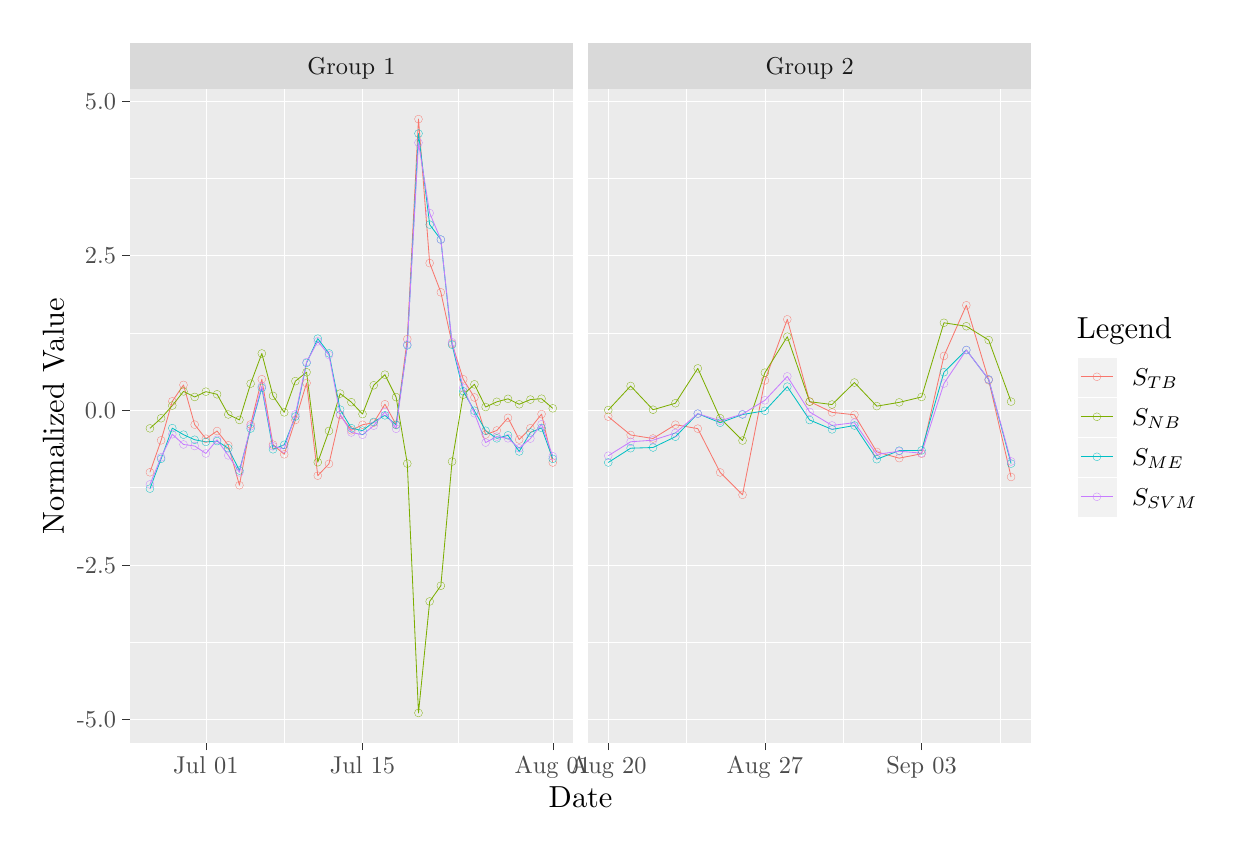
\begin{tikzpicture}[x=1pt,y=1pt]
\definecolor{fillColor}{RGB}{255,255,255}
\path[use as bounding box,fill=fillColor,fill opacity=0.00] (0,0) rectangle (433.62,289.08);
\begin{scope}
\path[clip] (  0.00,  0.00) rectangle (433.62,289.08);
\definecolor{drawColor}{RGB}{255,255,255}
\definecolor{fillColor}{RGB}{255,255,255}

\path[draw=drawColor,line width= 0.1pt,line join=round,line cap=round,fill=fillColor] (  0.00,  0.00) rectangle (433.62,289.08);
\end{scope}
\begin{scope}
\path[clip] ( 36.90, 30.73) rectangle (197.01,266.77);
\definecolor{fillColor}{gray}{0.92}

\path[fill=fillColor] ( 36.90, 30.73) rectangle (197.01,266.77);
\definecolor{drawColor}{RGB}{255,255,255}

\path[draw=drawColor,line width= 0.1pt,line join=round] ( 36.90, 67.00) --
	(197.01, 67.00);

\path[draw=drawColor,line width= 0.1pt,line join=round] ( 36.90,122.89) --
	(197.01,122.89);

\path[draw=drawColor,line width= 0.1pt,line join=round] ( 36.90,178.79) --
	(197.01,178.79);

\path[draw=drawColor,line width= 0.1pt,line join=round] ( 36.90,234.68) --
	(197.01,234.68);

\path[draw=drawColor,line width= 0.1pt,line join=round] ( 92.70, 30.73) --
	( 92.70,266.77);

\path[draw=drawColor,line width= 0.1pt,line join=round] (155.37, 30.73) --
	(155.37,266.77);

\path[draw=drawColor,line width= 0.1pt,line join=round] ( 36.90, 39.05) --
	(197.01, 39.05);

\path[draw=drawColor,line width= 0.1pt,line join=round] ( 36.90, 94.95) --
	(197.01, 94.95);

\path[draw=drawColor,line width= 0.1pt,line join=round] ( 36.90,150.84) --
	(197.01,150.84);

\path[draw=drawColor,line width= 0.1pt,line join=round] ( 36.90,206.73) --
	(197.01,206.73);

\path[draw=drawColor,line width= 0.1pt,line join=round] ( 36.90,262.63) --
	(197.01,262.63);

\path[draw=drawColor,line width= 0.1pt,line join=round] ( 64.39, 30.73) --
	( 64.39,266.77);

\path[draw=drawColor,line width= 0.1pt,line join=round] (121.00, 30.73) --
	(121.00,266.77);

\path[draw=drawColor,line width= 0.1pt,line join=round] (189.74, 30.73) --
	(189.74,266.77);
\definecolor{drawColor}{RGB}{248,118,109}

\path[draw=drawColor,line width= 0.3pt,line join=round] ( 44.18,128.42) --
	( 48.22,139.97) --
	( 52.26,154.07) --
	( 56.31,159.99) --
	( 60.35,145.63) --
	( 64.39,140.54) --
	( 68.44,143.33) --
	( 72.48,138.19) --
	( 76.52,123.74) --
	( 80.57,145.71) --
	( 84.61,162.05) --
	( 88.65,138.42) --
	( 92.70,134.91) --
	( 96.74,147.31) --
	(100.78,160.65) --
	(104.83,127.19) --
	(108.87,131.47) --
	(112.91,149.12) --
	(116.96,143.59) --
	(121.00,145.58) --
	(125.04,146.35) --
	(129.09,153.00) --
	(133.13,145.64) --
	(137.17,176.53) --
	(141.22,256.04) --
	(145.26,204.01) --
	(149.30,193.46) --
	(153.35,174.91) --
	(157.39,162.04) --
	(161.43,155.46) --
	(165.48,142.05) --
	(169.52,143.52) --
	(173.56,148.10) --
	(177.61,140.24) --
	(181.65,144.34) --
	(185.69,149.44) --
	(189.74,131.95);
\definecolor{drawColor}{RGB}{124,174,0}

\path[draw=drawColor,line width= 0.3pt,line join=round] ( 44.18,144.29) --
	( 48.22,147.95) --
	( 52.26,152.52) --
	( 56.31,157.64) --
	( 60.35,155.64) --
	( 64.39,157.55) --
	( 68.44,156.60) --
	( 72.48,149.32) --
	( 76.52,147.34) --
	( 80.57,160.45) --
	( 84.61,171.34) --
	( 88.65,156.03) --
	( 92.70,150.08) --
	( 96.74,161.36) --
	(100.78,164.58) --
	(104.83,132.05) --
	(108.87,143.36) --
	(112.91,156.86) --
	(116.96,153.75) --
	(121.00,149.45) --
	(125.04,159.86) --
	(129.09,163.69) --
	(133.13,155.58) --
	(137.17,131.56) --
	(141.22, 41.46) --
	(145.26, 81.74) --
	(149.30, 87.42) --
	(153.35,132.29) --
	(157.39,156.46) --
	(161.43,160.20) --
	(165.48,151.99) --
	(169.52,153.88) --
	(173.56,154.96) --
	(177.61,152.99) --
	(181.65,154.69) --
	(185.69,155.01) --
	(189.74,151.53);
\definecolor{drawColor}{RGB}{0,191,196}

\path[draw=drawColor,line width= 0.3pt,line join=round] ( 44.18,122.50) --
	( 48.22,133.29) --
	( 52.26,144.37) --
	( 56.31,142.01) --
	( 60.35,140.17) --
	( 64.39,139.40) --
	( 68.44,139.69) --
	( 72.48,137.11) --
	( 76.52,129.05) --
	( 80.57,144.24) --
	( 84.61,158.93) --
	( 88.65,136.73) --
	( 92.70,138.35) --
	( 96.74,148.58) --
	(100.78,167.95) --
	(104.83,176.71) --
	(108.87,171.39) --
	(112.91,151.05) --
	(116.96,144.35) --
	(121.00,143.47) --
	(125.04,146.61) --
	(129.09,149.00) --
	(133.13,145.50) --
	(137.17,174.28) --
	(141.22,250.81) --
	(145.26,217.91) --
	(149.30,212.52) --
	(153.35,174.52) --
	(157.39,157.70) --
	(161.43,150.66) --
	(165.48,143.43) --
	(169.52,140.68) --
	(173.56,141.78) --
	(177.61,135.94) --
	(181.65,142.79) --
	(185.69,144.46) --
	(189.74,133.28);
\definecolor{drawColor}{RGB}{199,124,255}

\path[draw=drawColor,line width= 0.3pt,line join=round] ( 44.18,124.04) --
	( 48.22,133.83) --
	( 52.26,142.17) --
	( 56.31,138.47) --
	( 60.35,137.91) --
	( 64.39,135.21) --
	( 68.44,140.14) --
	( 72.48,134.53) --
	( 76.52,128.40) --
	( 80.57,145.03) --
	( 84.61,159.51) --
	( 88.65,137.80) --
	( 92.70,136.92) --
	( 96.74,149.36) --
	(100.78,168.23) --
	(104.83,175.74) --
	(108.87,170.80) --
	(112.91,149.30) --
	(116.96,142.81) --
	(121.00,141.98) --
	(125.04,145.26) --
	(129.09,150.23) --
	(133.13,144.14) --
	(137.17,174.61) --
	(141.22,247.51) --
	(145.26,222.08) --
	(149.30,212.47) --
	(153.35,175.40) --
	(157.39,158.96) --
	(161.43,149.76) --
	(165.48,139.15) --
	(169.52,141.31) --
	(173.56,140.70) --
	(177.61,137.09) --
	(181.65,140.60) --
	(185.69,145.78) --
	(189.74,134.21);
\definecolor{drawColor}{RGB}{248,118,109}

\path[draw=drawColor,line width= 0.1pt,line join=round,line cap=round] ( 44.18,128.42) circle (  1.43);

\path[draw=drawColor,line width= 0.1pt,line join=round,line cap=round] ( 48.22,139.97) circle (  1.43);

\path[draw=drawColor,line width= 0.1pt,line join=round,line cap=round] ( 52.26,154.07) circle (  1.43);

\path[draw=drawColor,line width= 0.1pt,line join=round,line cap=round] ( 56.31,159.99) circle (  1.43);

\path[draw=drawColor,line width= 0.1pt,line join=round,line cap=round] ( 60.35,145.63) circle (  1.43);

\path[draw=drawColor,line width= 0.1pt,line join=round,line cap=round] ( 64.39,140.54) circle (  1.43);

\path[draw=drawColor,line width= 0.1pt,line join=round,line cap=round] ( 68.44,143.33) circle (  1.43);

\path[draw=drawColor,line width= 0.1pt,line join=round,line cap=round] ( 72.48,138.19) circle (  1.43);

\path[draw=drawColor,line width= 0.1pt,line join=round,line cap=round] ( 76.52,123.74) circle (  1.43);

\path[draw=drawColor,line width= 0.1pt,line join=round,line cap=round] ( 80.57,145.71) circle (  1.43);

\path[draw=drawColor,line width= 0.1pt,line join=round,line cap=round] ( 84.61,162.05) circle (  1.43);

\path[draw=drawColor,line width= 0.1pt,line join=round,line cap=round] ( 88.65,138.42) circle (  1.43);

\path[draw=drawColor,line width= 0.1pt,line join=round,line cap=round] ( 92.70,134.91) circle (  1.43);

\path[draw=drawColor,line width= 0.1pt,line join=round,line cap=round] ( 96.74,147.31) circle (  1.43);

\path[draw=drawColor,line width= 0.1pt,line join=round,line cap=round] (100.78,160.65) circle (  1.43);

\path[draw=drawColor,line width= 0.1pt,line join=round,line cap=round] (104.83,127.19) circle (  1.43);

\path[draw=drawColor,line width= 0.1pt,line join=round,line cap=round] (108.87,131.47) circle (  1.43);

\path[draw=drawColor,line width= 0.1pt,line join=round,line cap=round] (112.91,149.12) circle (  1.43);

\path[draw=drawColor,line width= 0.1pt,line join=round,line cap=round] (116.96,143.59) circle (  1.43);

\path[draw=drawColor,line width= 0.1pt,line join=round,line cap=round] (121.00,145.58) circle (  1.43);

\path[draw=drawColor,line width= 0.1pt,line join=round,line cap=round] (125.04,146.35) circle (  1.43);

\path[draw=drawColor,line width= 0.1pt,line join=round,line cap=round] (129.09,153.00) circle (  1.43);

\path[draw=drawColor,line width= 0.1pt,line join=round,line cap=round] (133.13,145.64) circle (  1.43);

\path[draw=drawColor,line width= 0.1pt,line join=round,line cap=round] (137.17,176.53) circle (  1.43);

\path[draw=drawColor,line width= 0.1pt,line join=round,line cap=round] (141.22,256.04) circle (  1.43);

\path[draw=drawColor,line width= 0.1pt,line join=round,line cap=round] (145.26,204.01) circle (  1.43);

\path[draw=drawColor,line width= 0.1pt,line join=round,line cap=round] (149.30,193.46) circle (  1.43);

\path[draw=drawColor,line width= 0.1pt,line join=round,line cap=round] (153.35,174.91) circle (  1.43);

\path[draw=drawColor,line width= 0.1pt,line join=round,line cap=round] (157.39,162.04) circle (  1.43);

\path[draw=drawColor,line width= 0.1pt,line join=round,line cap=round] (161.43,155.46) circle (  1.43);

\path[draw=drawColor,line width= 0.1pt,line join=round,line cap=round] (165.48,142.05) circle (  1.43);

\path[draw=drawColor,line width= 0.1pt,line join=round,line cap=round] (169.52,143.52) circle (  1.43);

\path[draw=drawColor,line width= 0.1pt,line join=round,line cap=round] (173.56,148.10) circle (  1.43);

\path[draw=drawColor,line width= 0.1pt,line join=round,line cap=round] (177.61,140.24) circle (  1.43);

\path[draw=drawColor,line width= 0.1pt,line join=round,line cap=round] (181.65,144.34) circle (  1.43);

\path[draw=drawColor,line width= 0.1pt,line join=round,line cap=round] (185.69,149.44) circle (  1.43);

\path[draw=drawColor,line width= 0.1pt,line join=round,line cap=round] (189.74,131.95) circle (  1.43);
\definecolor{drawColor}{RGB}{124,174,0}

\path[draw=drawColor,line width= 0.1pt,line join=round,line cap=round] ( 44.18,144.29) circle (  1.43);

\path[draw=drawColor,line width= 0.1pt,line join=round,line cap=round] ( 48.22,147.95) circle (  1.43);

\path[draw=drawColor,line width= 0.1pt,line join=round,line cap=round] ( 52.26,152.52) circle (  1.43);

\path[draw=drawColor,line width= 0.1pt,line join=round,line cap=round] ( 56.31,157.64) circle (  1.43);

\path[draw=drawColor,line width= 0.1pt,line join=round,line cap=round] ( 60.35,155.64) circle (  1.43);

\path[draw=drawColor,line width= 0.1pt,line join=round,line cap=round] ( 64.39,157.55) circle (  1.43);

\path[draw=drawColor,line width= 0.1pt,line join=round,line cap=round] ( 68.44,156.60) circle (  1.43);

\path[draw=drawColor,line width= 0.1pt,line join=round,line cap=round] ( 72.48,149.32) circle (  1.43);

\path[draw=drawColor,line width= 0.1pt,line join=round,line cap=round] ( 76.52,147.34) circle (  1.43);

\path[draw=drawColor,line width= 0.1pt,line join=round,line cap=round] ( 80.57,160.45) circle (  1.43);

\path[draw=drawColor,line width= 0.1pt,line join=round,line cap=round] ( 84.61,171.34) circle (  1.43);

\path[draw=drawColor,line width= 0.1pt,line join=round,line cap=round] ( 88.65,156.03) circle (  1.43);

\path[draw=drawColor,line width= 0.1pt,line join=round,line cap=round] ( 92.70,150.08) circle (  1.43);

\path[draw=drawColor,line width= 0.1pt,line join=round,line cap=round] ( 96.74,161.36) circle (  1.43);

\path[draw=drawColor,line width= 0.1pt,line join=round,line cap=round] (100.78,164.58) circle (  1.43);

\path[draw=drawColor,line width= 0.1pt,line join=round,line cap=round] (104.83,132.05) circle (  1.43);

\path[draw=drawColor,line width= 0.1pt,line join=round,line cap=round] (108.87,143.36) circle (  1.43);

\path[draw=drawColor,line width= 0.1pt,line join=round,line cap=round] (112.91,156.86) circle (  1.43);

\path[draw=drawColor,line width= 0.1pt,line join=round,line cap=round] (116.96,153.75) circle (  1.43);

\path[draw=drawColor,line width= 0.1pt,line join=round,line cap=round] (121.00,149.45) circle (  1.43);

\path[draw=drawColor,line width= 0.1pt,line join=round,line cap=round] (125.04,159.86) circle (  1.43);

\path[draw=drawColor,line width= 0.1pt,line join=round,line cap=round] (129.09,163.69) circle (  1.43);

\path[draw=drawColor,line width= 0.1pt,line join=round,line cap=round] (133.13,155.58) circle (  1.43);

\path[draw=drawColor,line width= 0.1pt,line join=round,line cap=round] (137.17,131.56) circle (  1.43);

\path[draw=drawColor,line width= 0.1pt,line join=round,line cap=round] (141.22, 41.46) circle (  1.43);

\path[draw=drawColor,line width= 0.1pt,line join=round,line cap=round] (145.26, 81.74) circle (  1.43);

\path[draw=drawColor,line width= 0.1pt,line join=round,line cap=round] (149.30, 87.42) circle (  1.43);

\path[draw=drawColor,line width= 0.1pt,line join=round,line cap=round] (153.35,132.29) circle (  1.43);

\path[draw=drawColor,line width= 0.1pt,line join=round,line cap=round] (157.39,156.46) circle (  1.43);

\path[draw=drawColor,line width= 0.1pt,line join=round,line cap=round] (161.43,160.20) circle (  1.43);

\path[draw=drawColor,line width= 0.1pt,line join=round,line cap=round] (165.48,151.99) circle (  1.43);

\path[draw=drawColor,line width= 0.1pt,line join=round,line cap=round] (169.52,153.88) circle (  1.43);

\path[draw=drawColor,line width= 0.1pt,line join=round,line cap=round] (173.56,154.96) circle (  1.43);

\path[draw=drawColor,line width= 0.1pt,line join=round,line cap=round] (177.61,152.99) circle (  1.43);

\path[draw=drawColor,line width= 0.1pt,line join=round,line cap=round] (181.65,154.69) circle (  1.43);

\path[draw=drawColor,line width= 0.1pt,line join=round,line cap=round] (185.69,155.01) circle (  1.43);

\path[draw=drawColor,line width= 0.1pt,line join=round,line cap=round] (189.74,151.53) circle (  1.43);
\definecolor{drawColor}{RGB}{0,191,196}

\path[draw=drawColor,line width= 0.1pt,line join=round,line cap=round] ( 44.18,122.50) circle (  1.43);

\path[draw=drawColor,line width= 0.1pt,line join=round,line cap=round] ( 48.22,133.29) circle (  1.43);

\path[draw=drawColor,line width= 0.1pt,line join=round,line cap=round] ( 52.26,144.37) circle (  1.43);

\path[draw=drawColor,line width= 0.1pt,line join=round,line cap=round] ( 56.31,142.01) circle (  1.43);

\path[draw=drawColor,line width= 0.1pt,line join=round,line cap=round] ( 60.35,140.17) circle (  1.43);

\path[draw=drawColor,line width= 0.1pt,line join=round,line cap=round] ( 64.39,139.40) circle (  1.43);

\path[draw=drawColor,line width= 0.1pt,line join=round,line cap=round] ( 68.44,139.69) circle (  1.43);

\path[draw=drawColor,line width= 0.1pt,line join=round,line cap=round] ( 72.48,137.11) circle (  1.43);

\path[draw=drawColor,line width= 0.1pt,line join=round,line cap=round] ( 76.52,129.05) circle (  1.43);

\path[draw=drawColor,line width= 0.1pt,line join=round,line cap=round] ( 80.57,144.24) circle (  1.43);

\path[draw=drawColor,line width= 0.1pt,line join=round,line cap=round] ( 84.61,158.93) circle (  1.43);

\path[draw=drawColor,line width= 0.1pt,line join=round,line cap=round] ( 88.65,136.73) circle (  1.43);

\path[draw=drawColor,line width= 0.1pt,line join=round,line cap=round] ( 92.70,138.35) circle (  1.43);

\path[draw=drawColor,line width= 0.1pt,line join=round,line cap=round] ( 96.74,148.58) circle (  1.43);

\path[draw=drawColor,line width= 0.1pt,line join=round,line cap=round] (100.78,167.95) circle (  1.43);

\path[draw=drawColor,line width= 0.1pt,line join=round,line cap=round] (104.83,176.71) circle (  1.43);

\path[draw=drawColor,line width= 0.1pt,line join=round,line cap=round] (108.87,171.39) circle (  1.43);

\path[draw=drawColor,line width= 0.1pt,line join=round,line cap=round] (112.91,151.05) circle (  1.43);

\path[draw=drawColor,line width= 0.1pt,line join=round,line cap=round] (116.96,144.35) circle (  1.43);

\path[draw=drawColor,line width= 0.1pt,line join=round,line cap=round] (121.00,143.47) circle (  1.43);

\path[draw=drawColor,line width= 0.1pt,line join=round,line cap=round] (125.04,146.61) circle (  1.43);

\path[draw=drawColor,line width= 0.1pt,line join=round,line cap=round] (129.09,149.00) circle (  1.43);

\path[draw=drawColor,line width= 0.1pt,line join=round,line cap=round] (133.13,145.50) circle (  1.43);

\path[draw=drawColor,line width= 0.1pt,line join=round,line cap=round] (137.17,174.28) circle (  1.43);

\path[draw=drawColor,line width= 0.1pt,line join=round,line cap=round] (141.22,250.81) circle (  1.43);

\path[draw=drawColor,line width= 0.1pt,line join=round,line cap=round] (145.26,217.91) circle (  1.43);

\path[draw=drawColor,line width= 0.1pt,line join=round,line cap=round] (149.30,212.52) circle (  1.43);

\path[draw=drawColor,line width= 0.1pt,line join=round,line cap=round] (153.35,174.52) circle (  1.43);

\path[draw=drawColor,line width= 0.1pt,line join=round,line cap=round] (157.39,157.70) circle (  1.43);

\path[draw=drawColor,line width= 0.1pt,line join=round,line cap=round] (161.43,150.66) circle (  1.43);

\path[draw=drawColor,line width= 0.1pt,line join=round,line cap=round] (165.48,143.43) circle (  1.43);

\path[draw=drawColor,line width= 0.1pt,line join=round,line cap=round] (169.52,140.68) circle (  1.43);

\path[draw=drawColor,line width= 0.1pt,line join=round,line cap=round] (173.56,141.78) circle (  1.43);

\path[draw=drawColor,line width= 0.1pt,line join=round,line cap=round] (177.61,135.94) circle (  1.43);

\path[draw=drawColor,line width= 0.1pt,line join=round,line cap=round] (181.65,142.79) circle (  1.43);

\path[draw=drawColor,line width= 0.1pt,line join=round,line cap=round] (185.69,144.46) circle (  1.43);

\path[draw=drawColor,line width= 0.1pt,line join=round,line cap=round] (189.74,133.28) circle (  1.43);
\definecolor{drawColor}{RGB}{199,124,255}

\path[draw=drawColor,line width= 0.1pt,line join=round,line cap=round] ( 44.18,124.04) circle (  1.43);

\path[draw=drawColor,line width= 0.1pt,line join=round,line cap=round] ( 48.22,133.83) circle (  1.43);

\path[draw=drawColor,line width= 0.1pt,line join=round,line cap=round] ( 52.26,142.17) circle (  1.43);

\path[draw=drawColor,line width= 0.1pt,line join=round,line cap=round] ( 56.31,138.47) circle (  1.43);

\path[draw=drawColor,line width= 0.1pt,line join=round,line cap=round] ( 60.35,137.91) circle (  1.43);

\path[draw=drawColor,line width= 0.1pt,line join=round,line cap=round] ( 64.39,135.21) circle (  1.43);

\path[draw=drawColor,line width= 0.1pt,line join=round,line cap=round] ( 68.44,140.14) circle (  1.43);

\path[draw=drawColor,line width= 0.1pt,line join=round,line cap=round] ( 72.48,134.53) circle (  1.43);

\path[draw=drawColor,line width= 0.1pt,line join=round,line cap=round] ( 76.52,128.40) circle (  1.43);

\path[draw=drawColor,line width= 0.1pt,line join=round,line cap=round] ( 80.57,145.03) circle (  1.43);

\path[draw=drawColor,line width= 0.1pt,line join=round,line cap=round] ( 84.61,159.51) circle (  1.43);

\path[draw=drawColor,line width= 0.1pt,line join=round,line cap=round] ( 88.65,137.80) circle (  1.43);

\path[draw=drawColor,line width= 0.1pt,line join=round,line cap=round] ( 92.70,136.92) circle (  1.43);

\path[draw=drawColor,line width= 0.1pt,line join=round,line cap=round] ( 96.74,149.36) circle (  1.43);

\path[draw=drawColor,line width= 0.1pt,line join=round,line cap=round] (100.78,168.23) circle (  1.43);

\path[draw=drawColor,line width= 0.1pt,line join=round,line cap=round] (104.83,175.74) circle (  1.43);

\path[draw=drawColor,line width= 0.1pt,line join=round,line cap=round] (108.87,170.80) circle (  1.43);

\path[draw=drawColor,line width= 0.1pt,line join=round,line cap=round] (112.91,149.30) circle (  1.43);

\path[draw=drawColor,line width= 0.1pt,line join=round,line cap=round] (116.96,142.81) circle (  1.43);

\path[draw=drawColor,line width= 0.1pt,line join=round,line cap=round] (121.00,141.98) circle (  1.43);

\path[draw=drawColor,line width= 0.1pt,line join=round,line cap=round] (125.04,145.26) circle (  1.43);

\path[draw=drawColor,line width= 0.1pt,line join=round,line cap=round] (129.09,150.23) circle (  1.43);

\path[draw=drawColor,line width= 0.1pt,line join=round,line cap=round] (133.13,144.14) circle (  1.43);

\path[draw=drawColor,line width= 0.1pt,line join=round,line cap=round] (137.17,174.61) circle (  1.43);

\path[draw=drawColor,line width= 0.1pt,line join=round,line cap=round] (141.22,247.51) circle (  1.43);

\path[draw=drawColor,line width= 0.1pt,line join=round,line cap=round] (145.26,222.08) circle (  1.43);

\path[draw=drawColor,line width= 0.1pt,line join=round,line cap=round] (149.30,212.47) circle (  1.43);

\path[draw=drawColor,line width= 0.1pt,line join=round,line cap=round] (153.35,175.40) circle (  1.43);

\path[draw=drawColor,line width= 0.1pt,line join=round,line cap=round] (157.39,158.96) circle (  1.43);

\path[draw=drawColor,line width= 0.1pt,line join=round,line cap=round] (161.43,149.76) circle (  1.43);

\path[draw=drawColor,line width= 0.1pt,line join=round,line cap=round] (165.48,139.15) circle (  1.43);

\path[draw=drawColor,line width= 0.1pt,line join=round,line cap=round] (169.52,141.31) circle (  1.43);

\path[draw=drawColor,line width= 0.1pt,line join=round,line cap=round] (173.56,140.70) circle (  1.43);

\path[draw=drawColor,line width= 0.1pt,line join=round,line cap=round] (177.61,137.09) circle (  1.43);

\path[draw=drawColor,line width= 0.1pt,line join=round,line cap=round] (181.65,140.60) circle (  1.43);

\path[draw=drawColor,line width= 0.1pt,line join=round,line cap=round] (185.69,145.78) circle (  1.43);

\path[draw=drawColor,line width= 0.1pt,line join=round,line cap=round] (189.74,134.21) circle (  1.43);
\end{scope}
\begin{scope}
\path[clip] (202.51, 30.73) rectangle (362.63,266.77);
\definecolor{fillColor}{gray}{0.92}

\path[fill=fillColor] (202.51, 30.73) rectangle (362.63,266.77);
\definecolor{drawColor}{RGB}{255,255,255}

\path[draw=drawColor,line width= 0.1pt,line join=round] (202.51, 67.00) --
	(362.63, 67.00);

\path[draw=drawColor,line width= 0.1pt,line join=round] (202.51,122.89) --
	(362.63,122.89);

\path[draw=drawColor,line width= 0.1pt,line join=round] (202.51,178.79) --
	(362.63,178.79);

\path[draw=drawColor,line width= 0.1pt,line join=round] (202.51,234.68) --
	(362.63,234.68);

\path[draw=drawColor,line width= 0.1pt,line join=round] (238.10, 30.73) --
	(238.10,266.77);

\path[draw=drawColor,line width= 0.1pt,line join=round] (294.70, 30.73) --
	(294.70,266.77);

\path[draw=drawColor,line width= 0.1pt,line join=round] (351.31, 30.73) --
	(351.31,266.77);

\path[draw=drawColor,line width= 0.1pt,line join=round] (202.51, 39.05) --
	(362.63, 39.05);

\path[draw=drawColor,line width= 0.1pt,line join=round] (202.51, 94.95) --
	(362.63, 94.95);

\path[draw=drawColor,line width= 0.1pt,line join=round] (202.51,150.84) --
	(362.63,150.84);

\path[draw=drawColor,line width= 0.1pt,line join=round] (202.51,206.73) --
	(362.63,206.73);

\path[draw=drawColor,line width= 0.1pt,line join=round] (202.51,262.63) --
	(362.63,262.63);

\path[draw=drawColor,line width= 0.1pt,line join=round] (209.79, 30.73) --
	(209.79,266.77);

\path[draw=drawColor,line width= 0.1pt,line join=round] (266.40, 30.73) --
	(266.40,266.77);

\path[draw=drawColor,line width= 0.1pt,line join=round] (323.01, 30.73) --
	(323.01,266.77);
\definecolor{drawColor}{RGB}{248,118,109}

\path[draw=drawColor,line width= 0.3pt,line join=round] (209.79,148.53) --
	(217.88,141.90) --
	(225.97,140.62) --
	(234.05,145.62) --
	(242.14,144.19) --
	(250.23,128.36) --
	(258.31,120.27) --
	(266.40,161.61) --
	(274.49,183.68) --
	(282.57,153.97) --
	(290.66,150.08) --
	(298.75,149.18) --
	(306.83,135.78) --
	(314.92,133.52) --
	(323.01,135.12) --
	(331.09,170.45) --
	(339.18,188.77) --
	(347.26,161.68) --
	(355.35,126.72);
\definecolor{drawColor}{RGB}{124,174,0}

\path[draw=drawColor,line width= 0.3pt,line join=round] (209.79,150.90) --
	(217.88,159.60) --
	(225.97,151.02) --
	(234.05,153.37) --
	(242.14,165.96) --
	(250.23,147.96) --
	(258.31,139.88) --
	(266.40,164.41) --
	(274.49,177.42) --
	(282.57,153.92) --
	(290.66,152.90) --
	(298.75,160.84) --
	(306.83,152.32) --
	(314.92,153.68) --
	(323.01,155.63) --
	(331.09,182.44) --
	(339.18,181.19) --
	(347.26,176.19) --
	(355.35,153.95);
\definecolor{drawColor}{RGB}{0,191,196}

\path[draw=drawColor,line width= 0.3pt,line join=round] (209.79,131.96) --
	(217.88,137.12) --
	(225.97,137.37) --
	(234.05,141.27) --
	(242.14,149.60) --
	(250.23,146.32) --
	(258.31,149.29) --
	(266.40,150.64) --
	(274.49,159.37) --
	(282.57,147.30) --
	(290.66,143.91) --
	(298.75,145.32) --
	(306.83,133.14) --
	(314.92,136.24) --
	(323.01,136.33) --
	(331.09,164.58) --
	(339.18,172.61) --
	(347.26,161.95) --
	(355.35,131.55);
\definecolor{drawColor}{RGB}{199,124,255}

\path[draw=drawColor,line width= 0.3pt,line join=round] (209.79,134.40) --
	(217.88,139.44) --
	(225.97,140.02) --
	(234.05,142.62) --
	(242.14,149.61) --
	(250.23,147.02) --
	(258.31,149.45) --
	(266.40,154.43) --
	(274.49,163.07) --
	(282.57,150.21) --
	(290.66,145.35) --
	(298.75,146.35) --
	(306.83,134.88) --
	(314.92,136.03) --
	(323.01,135.33) --
	(331.09,160.49) --
	(339.18,172.58) --
	(347.26,162.00) --
	(355.35,132.34);
\definecolor{drawColor}{RGB}{248,118,109}

\path[draw=drawColor,line width= 0.1pt,line join=round,line cap=round] (209.79,148.53) circle (  1.43);

\path[draw=drawColor,line width= 0.1pt,line join=round,line cap=round] (217.88,141.90) circle (  1.43);

\path[draw=drawColor,line width= 0.1pt,line join=round,line cap=round] (225.97,140.62) circle (  1.43);

\path[draw=drawColor,line width= 0.1pt,line join=round,line cap=round] (234.05,145.62) circle (  1.43);

\path[draw=drawColor,line width= 0.1pt,line join=round,line cap=round] (242.14,144.19) circle (  1.43);

\path[draw=drawColor,line width= 0.1pt,line join=round,line cap=round] (250.23,128.36) circle (  1.43);

\path[draw=drawColor,line width= 0.1pt,line join=round,line cap=round] (258.31,120.27) circle (  1.43);

\path[draw=drawColor,line width= 0.1pt,line join=round,line cap=round] (266.40,161.61) circle (  1.43);

\path[draw=drawColor,line width= 0.1pt,line join=round,line cap=round] (274.49,183.68) circle (  1.43);

\path[draw=drawColor,line width= 0.1pt,line join=round,line cap=round] (282.57,153.97) circle (  1.43);

\path[draw=drawColor,line width= 0.1pt,line join=round,line cap=round] (290.66,150.08) circle (  1.43);

\path[draw=drawColor,line width= 0.1pt,line join=round,line cap=round] (298.75,149.18) circle (  1.43);

\path[draw=drawColor,line width= 0.1pt,line join=round,line cap=round] (306.83,135.78) circle (  1.43);

\path[draw=drawColor,line width= 0.1pt,line join=round,line cap=round] (314.92,133.52) circle (  1.43);

\path[draw=drawColor,line width= 0.1pt,line join=round,line cap=round] (323.01,135.12) circle (  1.43);

\path[draw=drawColor,line width= 0.1pt,line join=round,line cap=round] (331.09,170.45) circle (  1.43);

\path[draw=drawColor,line width= 0.1pt,line join=round,line cap=round] (339.18,188.77) circle (  1.43);

\path[draw=drawColor,line width= 0.1pt,line join=round,line cap=round] (347.26,161.68) circle (  1.43);

\path[draw=drawColor,line width= 0.1pt,line join=round,line cap=round] (355.35,126.72) circle (  1.43);
\definecolor{drawColor}{RGB}{124,174,0}

\path[draw=drawColor,line width= 0.1pt,line join=round,line cap=round] (209.79,150.90) circle (  1.43);

\path[draw=drawColor,line width= 0.1pt,line join=round,line cap=round] (217.88,159.60) circle (  1.43);

\path[draw=drawColor,line width= 0.1pt,line join=round,line cap=round] (225.97,151.02) circle (  1.43);

\path[draw=drawColor,line width= 0.1pt,line join=round,line cap=round] (234.05,153.37) circle (  1.43);

\path[draw=drawColor,line width= 0.1pt,line join=round,line cap=round] (242.14,165.96) circle (  1.43);

\path[draw=drawColor,line width= 0.1pt,line join=round,line cap=round] (250.23,147.96) circle (  1.43);

\path[draw=drawColor,line width= 0.1pt,line join=round,line cap=round] (258.31,139.88) circle (  1.43);

\path[draw=drawColor,line width= 0.1pt,line join=round,line cap=round] (266.40,164.41) circle (  1.43);

\path[draw=drawColor,line width= 0.1pt,line join=round,line cap=round] (274.49,177.42) circle (  1.43);

\path[draw=drawColor,line width= 0.1pt,line join=round,line cap=round] (282.57,153.92) circle (  1.43);

\path[draw=drawColor,line width= 0.1pt,line join=round,line cap=round] (290.66,152.90) circle (  1.43);

\path[draw=drawColor,line width= 0.1pt,line join=round,line cap=round] (298.75,160.84) circle (  1.43);

\path[draw=drawColor,line width= 0.1pt,line join=round,line cap=round] (306.83,152.32) circle (  1.43);

\path[draw=drawColor,line width= 0.1pt,line join=round,line cap=round] (314.92,153.68) circle (  1.43);

\path[draw=drawColor,line width= 0.1pt,line join=round,line cap=round] (323.01,155.63) circle (  1.43);

\path[draw=drawColor,line width= 0.1pt,line join=round,line cap=round] (331.09,182.44) circle (  1.43);

\path[draw=drawColor,line width= 0.1pt,line join=round,line cap=round] (339.18,181.19) circle (  1.43);

\path[draw=drawColor,line width= 0.1pt,line join=round,line cap=round] (347.26,176.19) circle (  1.43);

\path[draw=drawColor,line width= 0.1pt,line join=round,line cap=round] (355.35,153.95) circle (  1.43);
\definecolor{drawColor}{RGB}{0,191,196}

\path[draw=drawColor,line width= 0.1pt,line join=round,line cap=round] (209.79,131.96) circle (  1.43);

\path[draw=drawColor,line width= 0.1pt,line join=round,line cap=round] (217.88,137.12) circle (  1.43);

\path[draw=drawColor,line width= 0.1pt,line join=round,line cap=round] (225.97,137.37) circle (  1.43);

\path[draw=drawColor,line width= 0.1pt,line join=round,line cap=round] (234.05,141.27) circle (  1.43);

\path[draw=drawColor,line width= 0.1pt,line join=round,line cap=round] (242.14,149.60) circle (  1.43);

\path[draw=drawColor,line width= 0.1pt,line join=round,line cap=round] (250.23,146.32) circle (  1.43);

\path[draw=drawColor,line width= 0.1pt,line join=round,line cap=round] (258.31,149.29) circle (  1.43);

\path[draw=drawColor,line width= 0.1pt,line join=round,line cap=round] (266.40,150.64) circle (  1.43);

\path[draw=drawColor,line width= 0.1pt,line join=round,line cap=round] (274.49,159.37) circle (  1.43);

\path[draw=drawColor,line width= 0.1pt,line join=round,line cap=round] (282.57,147.30) circle (  1.43);

\path[draw=drawColor,line width= 0.1pt,line join=round,line cap=round] (290.66,143.91) circle (  1.43);

\path[draw=drawColor,line width= 0.1pt,line join=round,line cap=round] (298.75,145.32) circle (  1.43);

\path[draw=drawColor,line width= 0.1pt,line join=round,line cap=round] (306.83,133.14) circle (  1.43);

\path[draw=drawColor,line width= 0.1pt,line join=round,line cap=round] (314.92,136.24) circle (  1.43);

\path[draw=drawColor,line width= 0.1pt,line join=round,line cap=round] (323.01,136.33) circle (  1.43);

\path[draw=drawColor,line width= 0.1pt,line join=round,line cap=round] (331.09,164.58) circle (  1.43);

\path[draw=drawColor,line width= 0.1pt,line join=round,line cap=round] (339.18,172.61) circle (  1.43);

\path[draw=drawColor,line width= 0.1pt,line join=round,line cap=round] (347.26,161.95) circle (  1.43);

\path[draw=drawColor,line width= 0.1pt,line join=round,line cap=round] (355.35,131.55) circle (  1.43);
\definecolor{drawColor}{RGB}{199,124,255}

\path[draw=drawColor,line width= 0.1pt,line join=round,line cap=round] (209.79,134.40) circle (  1.43);

\path[draw=drawColor,line width= 0.1pt,line join=round,line cap=round] (217.88,139.44) circle (  1.43);

\path[draw=drawColor,line width= 0.1pt,line join=round,line cap=round] (225.97,140.02) circle (  1.43);

\path[draw=drawColor,line width= 0.1pt,line join=round,line cap=round] (234.05,142.62) circle (  1.43);

\path[draw=drawColor,line width= 0.1pt,line join=round,line cap=round] (242.14,149.61) circle (  1.43);

\path[draw=drawColor,line width= 0.1pt,line join=round,line cap=round] (250.23,147.02) circle (  1.43);

\path[draw=drawColor,line width= 0.1pt,line join=round,line cap=round] (258.31,149.45) circle (  1.43);

\path[draw=drawColor,line width= 0.1pt,line join=round,line cap=round] (266.40,154.43) circle (  1.43);

\path[draw=drawColor,line width= 0.1pt,line join=round,line cap=round] (274.49,163.07) circle (  1.43);

\path[draw=drawColor,line width= 0.1pt,line join=round,line cap=round] (282.57,150.21) circle (  1.43);

\path[draw=drawColor,line width= 0.1pt,line join=round,line cap=round] (290.66,145.35) circle (  1.43);

\path[draw=drawColor,line width= 0.1pt,line join=round,line cap=round] (298.75,146.35) circle (  1.43);

\path[draw=drawColor,line width= 0.1pt,line join=round,line cap=round] (306.83,134.88) circle (  1.43);

\path[draw=drawColor,line width= 0.1pt,line join=round,line cap=round] (314.92,136.03) circle (  1.43);

\path[draw=drawColor,line width= 0.1pt,line join=round,line cap=round] (323.01,135.33) circle (  1.43);

\path[draw=drawColor,line width= 0.1pt,line join=round,line cap=round] (331.09,160.49) circle (  1.43);

\path[draw=drawColor,line width= 0.1pt,line join=round,line cap=round] (339.18,172.58) circle (  1.43);

\path[draw=drawColor,line width= 0.1pt,line join=round,line cap=round] (347.26,162.00) circle (  1.43);

\path[draw=drawColor,line width= 0.1pt,line join=round,line cap=round] (355.35,132.34) circle (  1.43);
\end{scope}
\begin{scope}
\path[clip] ( 36.90,266.77) rectangle (197.01,283.58);
\definecolor{fillColor}{gray}{0.85}

\path[fill=fillColor] ( 36.90,266.77) rectangle (197.01,283.58);
\definecolor{drawColor}{gray}{0.10}

\node[text=drawColor,anchor=base,inner sep=0pt, outer sep=0pt, scale=  0.88] at (116.96,272.15) {Group 1};
\end{scope}
\begin{scope}
\path[clip] (202.51,266.77) rectangle (362.63,283.58);
\definecolor{fillColor}{gray}{0.85}

\path[fill=fillColor] (202.51,266.77) rectangle (362.63,283.58);
\definecolor{drawColor}{gray}{0.10}

\node[text=drawColor,anchor=base,inner sep=0pt, outer sep=0pt, scale=  0.88] at (282.57,272.15) {Group 2};
\end{scope}
\begin{scope}
\path[clip] (  0.00,  0.00) rectangle (433.62,289.08);
\definecolor{drawColor}{gray}{0.20}

\path[draw=drawColor,line width= 0.1pt,line join=round] ( 64.39, 27.98) --
	( 64.39, 30.73);

\path[draw=drawColor,line width= 0.1pt,line join=round] (121.00, 27.98) --
	(121.00, 30.73);

\path[draw=drawColor,line width= 0.1pt,line join=round] (189.74, 27.98) --
	(189.74, 30.73);
\end{scope}
\begin{scope}
\path[clip] (  0.00,  0.00) rectangle (433.62,289.08);
\definecolor{drawColor}{gray}{0.30}

\node[text=drawColor,anchor=base,inner sep=0pt, outer sep=0pt, scale=  0.88] at ( 64.39, 19.72) {Jul 01};

\node[text=drawColor,anchor=base,inner sep=0pt, outer sep=0pt, scale=  0.88] at (121.00, 19.72) {Jul 15};

\node[text=drawColor,anchor=base,inner sep=0pt, outer sep=0pt, scale=  0.88] at (189.74, 19.72) {Aug 01};
\end{scope}
\begin{scope}
\path[clip] (  0.00,  0.00) rectangle (433.62,289.08);
\definecolor{drawColor}{gray}{0.20}

\path[draw=drawColor,line width= 0.1pt,line join=round] (209.79, 27.98) --
	(209.79, 30.73);

\path[draw=drawColor,line width= 0.1pt,line join=round] (266.40, 27.98) --
	(266.40, 30.73);

\path[draw=drawColor,line width= 0.1pt,line join=round] (323.01, 27.98) --
	(323.01, 30.73);
\end{scope}
\begin{scope}
\path[clip] (  0.00,  0.00) rectangle (433.62,289.08);
\definecolor{drawColor}{gray}{0.30}

\node[text=drawColor,anchor=base,inner sep=0pt, outer sep=0pt, scale=  0.88] at (209.79, 19.72) {Aug 20};

\node[text=drawColor,anchor=base,inner sep=0pt, outer sep=0pt, scale=  0.88] at (266.40, 19.72) {Aug 27};

\node[text=drawColor,anchor=base,inner sep=0pt, outer sep=0pt, scale=  0.88] at (323.01, 19.72) {Sep 03};
\end{scope}
\begin{scope}
\path[clip] (  0.00,  0.00) rectangle (433.62,289.08);
\definecolor{drawColor}{gray}{0.30}

\node[text=drawColor,anchor=base east,inner sep=0pt, outer sep=0pt, scale=  0.88] at ( 31.95, 36.02) {-5.0};

\node[text=drawColor,anchor=base east,inner sep=0pt, outer sep=0pt, scale=  0.88] at ( 31.95, 91.92) {-2.5};

\node[text=drawColor,anchor=base east,inner sep=0pt, outer sep=0pt, scale=  0.88] at ( 31.95,147.81) {0.0};

\node[text=drawColor,anchor=base east,inner sep=0pt, outer sep=0pt, scale=  0.88] at ( 31.95,203.70) {2.5};

\node[text=drawColor,anchor=base east,inner sep=0pt, outer sep=0pt, scale=  0.88] at ( 31.95,259.60) {5.0};
\end{scope}
\begin{scope}
\path[clip] (  0.00,  0.00) rectangle (433.62,289.08);
\definecolor{drawColor}{gray}{0.20}

\path[draw=drawColor,line width= 0.1pt,line join=round] ( 34.15, 39.05) --
	( 36.90, 39.05);

\path[draw=drawColor,line width= 0.1pt,line join=round] ( 34.15, 94.95) --
	( 36.90, 94.95);

\path[draw=drawColor,line width= 0.1pt,line join=round] ( 34.15,150.84) --
	( 36.90,150.84);

\path[draw=drawColor,line width= 0.1pt,line join=round] ( 34.15,206.73) --
	( 36.90,206.73);

\path[draw=drawColor,line width= 0.1pt,line join=round] ( 34.15,262.63) --
	( 36.90,262.63);
\end{scope}
\begin{scope}
\path[clip] (  0.00,  0.00) rectangle (433.62,289.08);
\definecolor{drawColor}{RGB}{0,0,0}

\node[text=drawColor,anchor=base,inner sep=0pt, outer sep=0pt, scale=  1.10] at (199.76,  7.44) {Date};
\end{scope}
\begin{scope}
\path[clip] (  0.00,  0.00) rectangle (433.62,289.08);
\definecolor{drawColor}{RGB}{0,0,0}

\node[text=drawColor,rotate= 90.00,anchor=base,inner sep=0pt, outer sep=0pt, scale=  1.10] at ( 13.08,148.75) {Normalized Value};
\end{scope}
\begin{scope}
\path[clip] (  0.00,  0.00) rectangle (433.62,289.08);
\definecolor{fillColor}{RGB}{255,255,255}

\path[fill=fillColor] (373.63,106.83) rectangle (428.12,190.67);
\end{scope}
\begin{scope}
\path[clip] (  0.00,  0.00) rectangle (433.62,289.08);
\definecolor{drawColor}{RGB}{0,0,0}

\node[text=drawColor,anchor=base west,inner sep=0pt, outer sep=0pt, scale=  1.10] at (379.13,176.62) {Legend};
\end{scope}
\begin{scope}
\path[clip] (  0.00,  0.00) rectangle (433.62,289.08);
\definecolor{drawColor}{RGB}{255,255,255}
\definecolor{fillColor}{gray}{0.95}

\path[draw=drawColor,line width= 0.1pt,line join=round,line cap=round,fill=fillColor] (379.13,155.69) rectangle (393.58,170.15);
\end{scope}
\begin{scope}
\path[clip] (  0.00,  0.00) rectangle (433.62,289.08);
\definecolor{drawColor}{RGB}{248,118,109}

\path[draw=drawColor,line width= 0.3pt,line join=round] (380.57,162.92) -- (392.14,162.92);
\end{scope}
\begin{scope}
\path[clip] (  0.00,  0.00) rectangle (433.62,289.08);
\definecolor{drawColor}{RGB}{248,118,109}

\path[draw=drawColor,line width= 0.1pt,line join=round,line cap=round] (386.36,162.92) circle (  1.43);
\end{scope}
\begin{scope}
\path[clip] (  0.00,  0.00) rectangle (433.62,289.08);
\definecolor{drawColor}{RGB}{255,255,255}
\definecolor{fillColor}{gray}{0.95}

\path[draw=drawColor,line width= 0.1pt,line join=round,line cap=round,fill=fillColor] (379.13,141.24) rectangle (393.58,155.69);
\end{scope}
\begin{scope}
\path[clip] (  0.00,  0.00) rectangle (433.62,289.08);
\definecolor{drawColor}{RGB}{124,174,0}

\path[draw=drawColor,line width= 0.3pt,line join=round] (380.57,148.47) -- (392.14,148.47);
\end{scope}
\begin{scope}
\path[clip] (  0.00,  0.00) rectangle (433.62,289.08);
\definecolor{drawColor}{RGB}{124,174,0}

\path[draw=drawColor,line width= 0.1pt,line join=round,line cap=round] (386.36,148.47) circle (  1.43);
\end{scope}
\begin{scope}
\path[clip] (  0.00,  0.00) rectangle (433.62,289.08);
\definecolor{drawColor}{RGB}{255,255,255}
\definecolor{fillColor}{gray}{0.95}

\path[draw=drawColor,line width= 0.1pt,line join=round,line cap=round,fill=fillColor] (379.13,126.79) rectangle (393.58,141.24);
\end{scope}
\begin{scope}
\path[clip] (  0.00,  0.00) rectangle (433.62,289.08);
\definecolor{drawColor}{RGB}{0,191,196}

\path[draw=drawColor,line width= 0.3pt,line join=round] (380.57,134.01) -- (392.14,134.01);
\end{scope}
\begin{scope}
\path[clip] (  0.00,  0.00) rectangle (433.62,289.08);
\definecolor{drawColor}{RGB}{0,191,196}

\path[draw=drawColor,line width= 0.1pt,line join=round,line cap=round] (386.36,134.01) circle (  1.43);
\end{scope}
\begin{scope}
\path[clip] (  0.00,  0.00) rectangle (433.62,289.08);
\definecolor{drawColor}{RGB}{255,255,255}
\definecolor{fillColor}{gray}{0.95}

\path[draw=drawColor,line width= 0.1pt,line join=round,line cap=round,fill=fillColor] (379.13,112.33) rectangle (393.58,126.79);
\end{scope}
\begin{scope}
\path[clip] (  0.00,  0.00) rectangle (433.62,289.08);
\definecolor{drawColor}{RGB}{199,124,255}

\path[draw=drawColor,line width= 0.3pt,line join=round] (380.57,119.56) -- (392.14,119.56);
\end{scope}
\begin{scope}
\path[clip] (  0.00,  0.00) rectangle (433.62,289.08);
\definecolor{drawColor}{RGB}{199,124,255}

\path[draw=drawColor,line width= 0.1pt,line join=round,line cap=round] (386.36,119.56) circle (  1.43);
\end{scope}
\begin{scope}
\path[clip] (  0.00,  0.00) rectangle (433.62,289.08);
\definecolor{drawColor}{RGB}{0,0,0}

\node[text=drawColor,anchor=base west,inner sep=0pt, outer sep=0pt, scale=  0.88] at (399.08,159.89) {$S_{TB}$};
\end{scope}
\begin{scope}
\path[clip] (  0.00,  0.00) rectangle (433.62,289.08);
\definecolor{drawColor}{RGB}{0,0,0}

\node[text=drawColor,anchor=base west,inner sep=0pt, outer sep=0pt, scale=  0.88] at (399.08,145.44) {$S_{NB}$};
\end{scope}
\begin{scope}
\path[clip] (  0.00,  0.00) rectangle (433.62,289.08);
\definecolor{drawColor}{RGB}{0,0,0}

\node[text=drawColor,anchor=base west,inner sep=0pt, outer sep=0pt, scale=  0.88] at (399.08,130.98) {$S_{ME}$};
\end{scope}
\begin{scope}
\path[clip] (  0.00,  0.00) rectangle (433.62,289.08);
\definecolor{drawColor}{RGB}{0,0,0}

\node[text=drawColor,anchor=base west,inner sep=0pt, outer sep=0pt, scale=  0.88] at (399.08,116.53) {$S_{SVM}$};
\end{scope}
\end{tikzpicture}

    \caption{\sentimentsCaption{\toyota}}
    \label{fig:analysis-sentiments-toyota}
\end{figure} 

\subsection{\vw}
\label{ss:analysis-sentiments-vw}

\begin{figure}[hbt]
    \centering
    % Created by tikzDevice version 0.12 on 2019-03-18 14:40:43
% !TEX encoding = UTF-8 Unicode
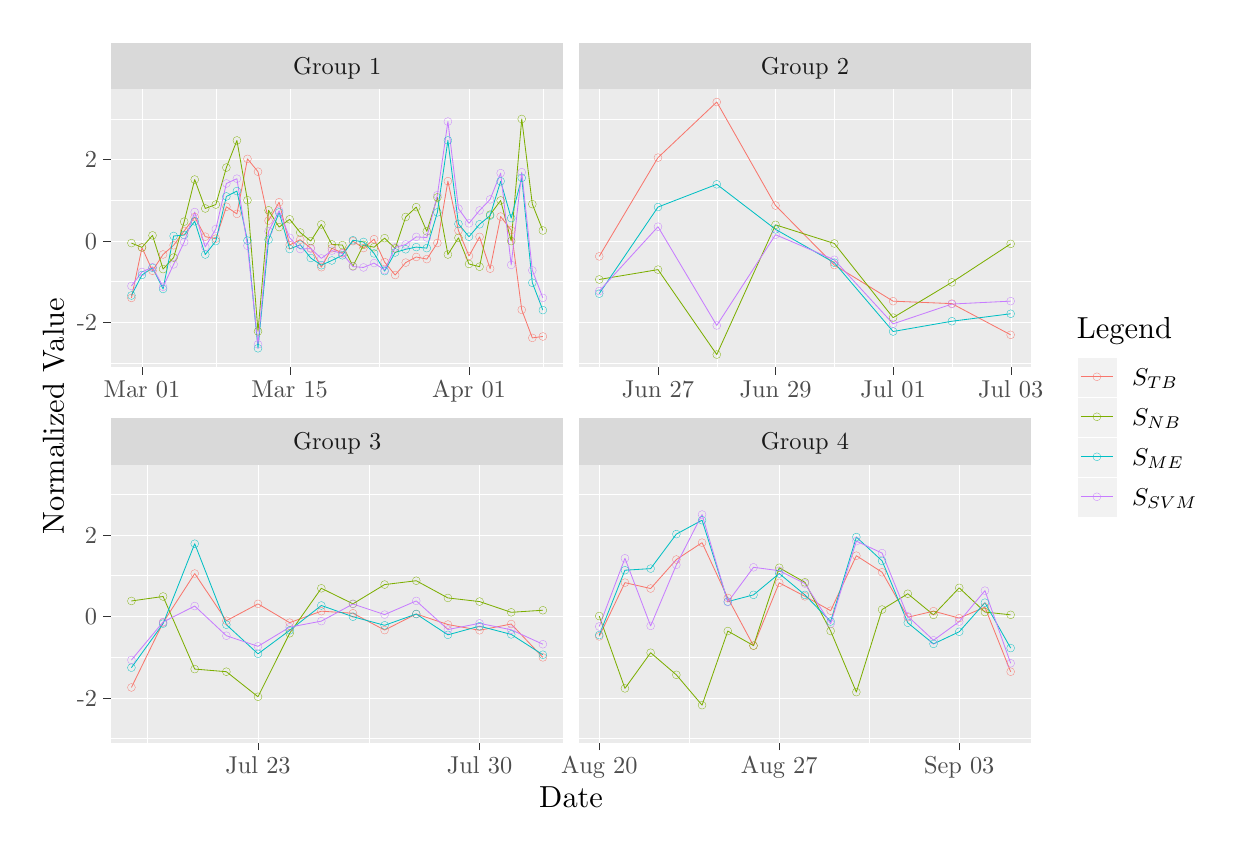
\begin{tikzpicture}[x=1pt,y=1pt]
\definecolor{fillColor}{RGB}{255,255,255}
\path[use as bounding box,fill=fillColor,fill opacity=0.00] (0,0) rectangle (433.62,289.08);
\begin{scope}
\path[clip] (  0.00,  0.00) rectangle (433.62,289.08);
\definecolor{drawColor}{RGB}{255,255,255}
\definecolor{fillColor}{RGB}{255,255,255}

\path[draw=drawColor,line width= 0.1pt,line join=round,line cap=round,fill=fillColor] (  0.00,  0.00) rectangle (433.62,289.08);
\end{scope}
\begin{scope}
\path[clip] ( 30.06,166.38) rectangle (193.59,266.77);
\definecolor{fillColor}{gray}{0.92}

\path[fill=fillColor] ( 30.06,166.38) rectangle (193.59,266.77);
\definecolor{drawColor}{RGB}{255,255,255}

\path[draw=drawColor,line width= 0.1pt,line join=round] ( 30.06,167.90) --
	(193.59,167.90);

\path[draw=drawColor,line width= 0.1pt,line join=round] ( 30.06,197.33) --
	(193.59,197.33);

\path[draw=drawColor,line width= 0.1pt,line join=round] ( 30.06,226.76) --
	(193.59,226.76);

\path[draw=drawColor,line width= 0.1pt,line join=round] ( 30.06,256.20) --
	(193.59,256.20);

\path[draw=drawColor,line width= 0.1pt,line join=round] ( 67.99,166.38) --
	( 67.99,266.77);

\path[draw=drawColor,line width= 0.1pt,line join=round] (127.07,166.38) --
	(127.07,266.77);

\path[draw=drawColor,line width= 0.1pt,line join=round] (186.16,166.38) --
	(186.16,266.77);

\path[draw=drawColor,line width= 0.1pt,line join=round] ( 30.06,182.62) --
	(193.59,182.62);

\path[draw=drawColor,line width= 0.1pt,line join=round] ( 30.06,212.05) --
	(193.59,212.05);

\path[draw=drawColor,line width= 0.1pt,line join=round] ( 30.06,241.48) --
	(193.59,241.48);

\path[draw=drawColor,line width= 0.1pt,line join=round] ( 41.30,166.38) --
	( 41.30,266.77);

\path[draw=drawColor,line width= 0.1pt,line join=round] ( 94.67,166.38) --
	( 94.67,266.77);

\path[draw=drawColor,line width= 0.1pt,line join=round] (159.47,166.38) --
	(159.47,266.77);
\definecolor{drawColor}{RGB}{248,118,109}

\path[draw=drawColor,line width= 0.3pt,line join=round] ( 37.49,191.42) --
	( 41.30,209.59) --
	( 45.11,201.23) --
	( 48.93,207.13) --
	( 52.74,210.44) --
	( 56.55,215.63) --
	( 60.36,220.64) --
	( 64.17,213.55) --
	( 67.99,212.85) --
	( 71.80,224.35) --
	( 75.61,221.79) --
	( 79.42,241.68) --
	( 83.23,237.02) --
	( 87.05,219.35) --
	( 90.86,226.01) --
	( 94.67,210.55) --
	( 98.48,212.45) --
	(102.29,209.41) --
	(106.11,202.53) --
	(109.92,209.36) --
	(113.73,207.69) --
	(117.54,211.93) --
	(121.35,209.45) --
	(125.17,212.65) --
	(128.98,204.37) --
	(132.79,199.69) --
	(136.60,204.19) --
	(140.41,206.22) --
	(144.23,205.44) --
	(148.04,211.27) --
	(151.85,233.62) --
	(155.66,215.74) --
	(159.47,206.58) --
	(163.29,213.48) --
	(167.10,201.98) --
	(170.91,220.82) --
	(174.72,215.92) --
	(178.53,187.12) --
	(182.35,176.98) --
	(186.16,177.49);
\definecolor{drawColor}{RGB}{124,174,0}

\path[draw=drawColor,line width= 0.3pt,line join=round] ( 37.49,211.24) --
	( 41.30,209.69) --
	( 45.11,214.02) --
	( 48.93,201.84) --
	( 52.74,206.00) --
	( 56.55,218.98) --
	( 60.36,234.20) --
	( 64.17,223.75) --
	( 67.99,225.16) --
	( 71.80,238.53) --
	( 75.61,248.32) --
	( 79.42,226.73) --
	( 83.23,179.35) --
	( 87.05,223.09) --
	( 90.86,217.02) --
	( 94.67,219.83) --
	( 98.48,215.07) --
	(102.29,211.96) --
	(106.11,217.97) --
	(109.92,210.75) --
	(113.73,210.51) --
	(117.54,202.91) --
	(121.35,210.58) --
	(125.17,209.75) --
	(128.98,213.02) --
	(132.79,209.29) --
	(136.60,220.67) --
	(140.41,224.24) --
	(144.23,215.49) --
	(148.04,227.75) --
	(151.85,207.11) --
	(155.66,213.14) --
	(159.47,203.68) --
	(163.29,202.70) --
	(167.10,221.50) --
	(170.91,226.65) --
	(174.72,211.98) --
	(178.53,256.08) --
	(182.35,225.32) --
	(186.16,215.78);
\definecolor{drawColor}{RGB}{0,191,196}

\path[draw=drawColor,line width= 0.3pt,line join=round] ( 37.49,192.30) --
	( 41.30,199.71) --
	( 45.11,202.31) --
	( 48.93,194.66) --
	( 52.74,213.79) --
	( 56.55,214.16) --
	( 60.36,219.11) --
	( 64.17,207.11) --
	( 67.99,211.96) --
	( 71.80,228.09) --
	( 75.61,230.04) --
	( 79.42,212.13) --
	( 83.23,173.23) --
	( 87.05,212.46) --
	( 90.86,222.32) --
	( 94.67,209.11) --
	( 98.48,210.64) --
	(102.29,205.85) --
	(106.11,203.25) --
	(109.92,204.96) --
	(113.73,206.82) --
	(117.54,212.27) --
	(121.35,211.64) --
	(125.17,207.52) --
	(128.98,201.10) --
	(132.79,207.85) --
	(136.60,209.00) --
	(140.41,209.79) --
	(144.23,209.41) --
	(148.04,222.33) --
	(151.85,248.34) --
	(155.66,218.15) --
	(159.47,213.53) --
	(163.29,218.03) --
	(167.10,221.16) --
	(170.91,233.59) --
	(174.72,220.26) --
	(178.53,234.81) --
	(182.35,196.90) --
	(186.16,187.02);
\definecolor{drawColor}{RGB}{199,124,255}

\path[draw=drawColor,line width= 0.3pt,line join=round] ( 37.49,195.74) --
	( 41.30,200.80) --
	( 45.11,202.52) --
	( 48.93,195.45) --
	( 52.74,203.54) --
	( 56.55,211.61) --
	( 60.36,222.45) --
	( 64.17,209.85) --
	( 67.99,216.32) --
	( 71.80,232.78) --
	( 75.61,234.51) --
	( 79.42,210.28) --
	( 83.23,174.63) --
	( 87.05,215.53) --
	( 90.86,222.90) --
	( 94.67,213.16) --
	( 98.48,209.08) --
	(102.29,209.24) --
	(106.11,205.70) --
	(109.92,208.51) --
	(113.73,207.47) --
	(117.54,202.74) --
	(121.35,202.44) --
	(125.17,204.02) --
	(128.98,201.49) --
	(132.79,209.68) --
	(136.60,210.72) --
	(140.41,213.48) --
	(144.23,213.25) --
	(148.04,228.56) --
	(151.85,255.15) --
	(155.66,223.70) --
	(159.47,218.38) --
	(163.29,223.03) --
	(167.10,227.02) --
	(170.91,236.52) --
	(174.72,203.34) --
	(178.53,236.85) --
	(182.35,201.39) --
	(186.16,191.44);
\definecolor{drawColor}{RGB}{248,118,109}

\path[draw=drawColor,line width= 0.1pt,line join=round,line cap=round] ( 37.49,191.42) circle (  1.43);

\path[draw=drawColor,line width= 0.1pt,line join=round,line cap=round] ( 41.30,209.59) circle (  1.43);

\path[draw=drawColor,line width= 0.1pt,line join=round,line cap=round] ( 45.11,201.23) circle (  1.43);

\path[draw=drawColor,line width= 0.1pt,line join=round,line cap=round] ( 48.93,207.13) circle (  1.43);

\path[draw=drawColor,line width= 0.1pt,line join=round,line cap=round] ( 52.74,210.44) circle (  1.43);

\path[draw=drawColor,line width= 0.1pt,line join=round,line cap=round] ( 56.55,215.63) circle (  1.43);

\path[draw=drawColor,line width= 0.1pt,line join=round,line cap=round] ( 60.36,220.64) circle (  1.43);

\path[draw=drawColor,line width= 0.1pt,line join=round,line cap=round] ( 64.17,213.55) circle (  1.43);

\path[draw=drawColor,line width= 0.1pt,line join=round,line cap=round] ( 67.99,212.85) circle (  1.43);

\path[draw=drawColor,line width= 0.1pt,line join=round,line cap=round] ( 71.80,224.35) circle (  1.43);

\path[draw=drawColor,line width= 0.1pt,line join=round,line cap=round] ( 75.61,221.79) circle (  1.43);

\path[draw=drawColor,line width= 0.1pt,line join=round,line cap=round] ( 79.42,241.68) circle (  1.43);

\path[draw=drawColor,line width= 0.1pt,line join=round,line cap=round] ( 83.23,237.02) circle (  1.43);

\path[draw=drawColor,line width= 0.1pt,line join=round,line cap=round] ( 87.05,219.35) circle (  1.43);

\path[draw=drawColor,line width= 0.1pt,line join=round,line cap=round] ( 90.86,226.01) circle (  1.43);

\path[draw=drawColor,line width= 0.1pt,line join=round,line cap=round] ( 94.67,210.55) circle (  1.43);

\path[draw=drawColor,line width= 0.1pt,line join=round,line cap=round] ( 98.48,212.45) circle (  1.43);

\path[draw=drawColor,line width= 0.1pt,line join=round,line cap=round] (102.29,209.41) circle (  1.43);

\path[draw=drawColor,line width= 0.1pt,line join=round,line cap=round] (106.11,202.53) circle (  1.43);

\path[draw=drawColor,line width= 0.1pt,line join=round,line cap=round] (109.92,209.36) circle (  1.43);

\path[draw=drawColor,line width= 0.1pt,line join=round,line cap=round] (113.73,207.69) circle (  1.43);

\path[draw=drawColor,line width= 0.1pt,line join=round,line cap=round] (117.54,211.93) circle (  1.43);

\path[draw=drawColor,line width= 0.1pt,line join=round,line cap=round] (121.35,209.45) circle (  1.43);

\path[draw=drawColor,line width= 0.1pt,line join=round,line cap=round] (125.17,212.65) circle (  1.43);

\path[draw=drawColor,line width= 0.1pt,line join=round,line cap=round] (128.98,204.37) circle (  1.43);

\path[draw=drawColor,line width= 0.1pt,line join=round,line cap=round] (132.79,199.69) circle (  1.43);

\path[draw=drawColor,line width= 0.1pt,line join=round,line cap=round] (136.60,204.19) circle (  1.43);

\path[draw=drawColor,line width= 0.1pt,line join=round,line cap=round] (140.41,206.22) circle (  1.43);

\path[draw=drawColor,line width= 0.1pt,line join=round,line cap=round] (144.23,205.44) circle (  1.43);

\path[draw=drawColor,line width= 0.1pt,line join=round,line cap=round] (148.04,211.27) circle (  1.43);

\path[draw=drawColor,line width= 0.1pt,line join=round,line cap=round] (151.85,233.62) circle (  1.43);

\path[draw=drawColor,line width= 0.1pt,line join=round,line cap=round] (155.66,215.74) circle (  1.43);

\path[draw=drawColor,line width= 0.1pt,line join=round,line cap=round] (159.47,206.58) circle (  1.43);

\path[draw=drawColor,line width= 0.1pt,line join=round,line cap=round] (163.29,213.48) circle (  1.43);

\path[draw=drawColor,line width= 0.1pt,line join=round,line cap=round] (167.10,201.98) circle (  1.43);

\path[draw=drawColor,line width= 0.1pt,line join=round,line cap=round] (170.91,220.82) circle (  1.43);

\path[draw=drawColor,line width= 0.1pt,line join=round,line cap=round] (174.72,215.92) circle (  1.43);

\path[draw=drawColor,line width= 0.1pt,line join=round,line cap=round] (178.53,187.12) circle (  1.43);

\path[draw=drawColor,line width= 0.1pt,line join=round,line cap=round] (182.35,176.98) circle (  1.43);

\path[draw=drawColor,line width= 0.1pt,line join=round,line cap=round] (186.16,177.49) circle (  1.43);
\definecolor{drawColor}{RGB}{124,174,0}

\path[draw=drawColor,line width= 0.1pt,line join=round,line cap=round] ( 37.49,211.24) circle (  1.43);

\path[draw=drawColor,line width= 0.1pt,line join=round,line cap=round] ( 41.30,209.69) circle (  1.43);

\path[draw=drawColor,line width= 0.1pt,line join=round,line cap=round] ( 45.11,214.02) circle (  1.43);

\path[draw=drawColor,line width= 0.1pt,line join=round,line cap=round] ( 48.93,201.84) circle (  1.43);

\path[draw=drawColor,line width= 0.1pt,line join=round,line cap=round] ( 52.74,206.00) circle (  1.43);

\path[draw=drawColor,line width= 0.1pt,line join=round,line cap=round] ( 56.55,218.98) circle (  1.43);

\path[draw=drawColor,line width= 0.1pt,line join=round,line cap=round] ( 60.36,234.20) circle (  1.43);

\path[draw=drawColor,line width= 0.1pt,line join=round,line cap=round] ( 64.17,223.75) circle (  1.43);

\path[draw=drawColor,line width= 0.1pt,line join=round,line cap=round] ( 67.99,225.16) circle (  1.43);

\path[draw=drawColor,line width= 0.1pt,line join=round,line cap=round] ( 71.80,238.53) circle (  1.43);

\path[draw=drawColor,line width= 0.1pt,line join=round,line cap=round] ( 75.61,248.32) circle (  1.43);

\path[draw=drawColor,line width= 0.1pt,line join=round,line cap=round] ( 79.42,226.73) circle (  1.43);

\path[draw=drawColor,line width= 0.1pt,line join=round,line cap=round] ( 83.23,179.35) circle (  1.43);

\path[draw=drawColor,line width= 0.1pt,line join=round,line cap=round] ( 87.05,223.09) circle (  1.43);

\path[draw=drawColor,line width= 0.1pt,line join=round,line cap=round] ( 90.86,217.02) circle (  1.43);

\path[draw=drawColor,line width= 0.1pt,line join=round,line cap=round] ( 94.67,219.83) circle (  1.43);

\path[draw=drawColor,line width= 0.1pt,line join=round,line cap=round] ( 98.48,215.07) circle (  1.43);

\path[draw=drawColor,line width= 0.1pt,line join=round,line cap=round] (102.29,211.96) circle (  1.43);

\path[draw=drawColor,line width= 0.1pt,line join=round,line cap=round] (106.11,217.97) circle (  1.43);

\path[draw=drawColor,line width= 0.1pt,line join=round,line cap=round] (109.92,210.75) circle (  1.43);

\path[draw=drawColor,line width= 0.1pt,line join=round,line cap=round] (113.73,210.51) circle (  1.43);

\path[draw=drawColor,line width= 0.1pt,line join=round,line cap=round] (117.54,202.91) circle (  1.43);

\path[draw=drawColor,line width= 0.1pt,line join=round,line cap=round] (121.35,210.58) circle (  1.43);

\path[draw=drawColor,line width= 0.1pt,line join=round,line cap=round] (125.17,209.75) circle (  1.43);

\path[draw=drawColor,line width= 0.1pt,line join=round,line cap=round] (128.98,213.02) circle (  1.43);

\path[draw=drawColor,line width= 0.1pt,line join=round,line cap=round] (132.79,209.29) circle (  1.43);

\path[draw=drawColor,line width= 0.1pt,line join=round,line cap=round] (136.60,220.67) circle (  1.43);

\path[draw=drawColor,line width= 0.1pt,line join=round,line cap=round] (140.41,224.24) circle (  1.43);

\path[draw=drawColor,line width= 0.1pt,line join=round,line cap=round] (144.23,215.49) circle (  1.43);

\path[draw=drawColor,line width= 0.1pt,line join=round,line cap=round] (148.04,227.75) circle (  1.43);

\path[draw=drawColor,line width= 0.1pt,line join=round,line cap=round] (151.85,207.11) circle (  1.43);

\path[draw=drawColor,line width= 0.1pt,line join=round,line cap=round] (155.66,213.14) circle (  1.43);

\path[draw=drawColor,line width= 0.1pt,line join=round,line cap=round] (159.47,203.68) circle (  1.43);

\path[draw=drawColor,line width= 0.1pt,line join=round,line cap=round] (163.29,202.70) circle (  1.43);

\path[draw=drawColor,line width= 0.1pt,line join=round,line cap=round] (167.10,221.50) circle (  1.43);

\path[draw=drawColor,line width= 0.1pt,line join=round,line cap=round] (170.91,226.65) circle (  1.43);

\path[draw=drawColor,line width= 0.1pt,line join=round,line cap=round] (174.72,211.98) circle (  1.43);

\path[draw=drawColor,line width= 0.1pt,line join=round,line cap=round] (178.53,256.08) circle (  1.43);

\path[draw=drawColor,line width= 0.1pt,line join=round,line cap=round] (182.35,225.32) circle (  1.43);

\path[draw=drawColor,line width= 0.1pt,line join=round,line cap=round] (186.16,215.78) circle (  1.43);
\definecolor{drawColor}{RGB}{0,191,196}

\path[draw=drawColor,line width= 0.1pt,line join=round,line cap=round] ( 37.49,192.30) circle (  1.43);

\path[draw=drawColor,line width= 0.1pt,line join=round,line cap=round] ( 41.30,199.71) circle (  1.43);

\path[draw=drawColor,line width= 0.1pt,line join=round,line cap=round] ( 45.11,202.31) circle (  1.43);

\path[draw=drawColor,line width= 0.1pt,line join=round,line cap=round] ( 48.93,194.66) circle (  1.43);

\path[draw=drawColor,line width= 0.1pt,line join=round,line cap=round] ( 52.74,213.79) circle (  1.43);

\path[draw=drawColor,line width= 0.1pt,line join=round,line cap=round] ( 56.55,214.16) circle (  1.43);

\path[draw=drawColor,line width= 0.1pt,line join=round,line cap=round] ( 60.36,219.11) circle (  1.43);

\path[draw=drawColor,line width= 0.1pt,line join=round,line cap=round] ( 64.17,207.11) circle (  1.43);

\path[draw=drawColor,line width= 0.1pt,line join=round,line cap=round] ( 67.99,211.96) circle (  1.43);

\path[draw=drawColor,line width= 0.1pt,line join=round,line cap=round] ( 71.80,228.09) circle (  1.43);

\path[draw=drawColor,line width= 0.1pt,line join=round,line cap=round] ( 75.61,230.04) circle (  1.43);

\path[draw=drawColor,line width= 0.1pt,line join=round,line cap=round] ( 79.42,212.13) circle (  1.43);

\path[draw=drawColor,line width= 0.1pt,line join=round,line cap=round] ( 83.23,173.23) circle (  1.43);

\path[draw=drawColor,line width= 0.1pt,line join=round,line cap=round] ( 87.05,212.46) circle (  1.43);

\path[draw=drawColor,line width= 0.1pt,line join=round,line cap=round] ( 90.86,222.32) circle (  1.43);

\path[draw=drawColor,line width= 0.1pt,line join=round,line cap=round] ( 94.67,209.11) circle (  1.43);

\path[draw=drawColor,line width= 0.1pt,line join=round,line cap=round] ( 98.48,210.64) circle (  1.43);

\path[draw=drawColor,line width= 0.1pt,line join=round,line cap=round] (102.29,205.85) circle (  1.43);

\path[draw=drawColor,line width= 0.1pt,line join=round,line cap=round] (106.11,203.25) circle (  1.43);

\path[draw=drawColor,line width= 0.1pt,line join=round,line cap=round] (109.92,204.96) circle (  1.43);

\path[draw=drawColor,line width= 0.1pt,line join=round,line cap=round] (113.73,206.82) circle (  1.43);

\path[draw=drawColor,line width= 0.1pt,line join=round,line cap=round] (117.54,212.27) circle (  1.43);

\path[draw=drawColor,line width= 0.1pt,line join=round,line cap=round] (121.35,211.64) circle (  1.43);

\path[draw=drawColor,line width= 0.1pt,line join=round,line cap=round] (125.17,207.52) circle (  1.43);

\path[draw=drawColor,line width= 0.1pt,line join=round,line cap=round] (128.98,201.10) circle (  1.43);

\path[draw=drawColor,line width= 0.1pt,line join=round,line cap=round] (132.79,207.85) circle (  1.43);

\path[draw=drawColor,line width= 0.1pt,line join=round,line cap=round] (136.60,209.00) circle (  1.43);

\path[draw=drawColor,line width= 0.1pt,line join=round,line cap=round] (140.41,209.79) circle (  1.43);

\path[draw=drawColor,line width= 0.1pt,line join=round,line cap=round] (144.23,209.41) circle (  1.43);

\path[draw=drawColor,line width= 0.1pt,line join=round,line cap=round] (148.04,222.33) circle (  1.43);

\path[draw=drawColor,line width= 0.1pt,line join=round,line cap=round] (151.85,248.34) circle (  1.43);

\path[draw=drawColor,line width= 0.1pt,line join=round,line cap=round] (155.66,218.15) circle (  1.43);

\path[draw=drawColor,line width= 0.1pt,line join=round,line cap=round] (159.47,213.53) circle (  1.43);

\path[draw=drawColor,line width= 0.1pt,line join=round,line cap=round] (163.29,218.03) circle (  1.43);

\path[draw=drawColor,line width= 0.1pt,line join=round,line cap=round] (167.10,221.16) circle (  1.43);

\path[draw=drawColor,line width= 0.1pt,line join=round,line cap=round] (170.91,233.59) circle (  1.43);

\path[draw=drawColor,line width= 0.1pt,line join=round,line cap=round] (174.72,220.26) circle (  1.43);

\path[draw=drawColor,line width= 0.1pt,line join=round,line cap=round] (178.53,234.81) circle (  1.43);

\path[draw=drawColor,line width= 0.1pt,line join=round,line cap=round] (182.35,196.90) circle (  1.43);

\path[draw=drawColor,line width= 0.1pt,line join=round,line cap=round] (186.16,187.02) circle (  1.43);
\definecolor{drawColor}{RGB}{199,124,255}

\path[draw=drawColor,line width= 0.1pt,line join=round,line cap=round] ( 37.49,195.74) circle (  1.43);

\path[draw=drawColor,line width= 0.1pt,line join=round,line cap=round] ( 41.30,200.80) circle (  1.43);

\path[draw=drawColor,line width= 0.1pt,line join=round,line cap=round] ( 45.11,202.52) circle (  1.43);

\path[draw=drawColor,line width= 0.1pt,line join=round,line cap=round] ( 48.93,195.45) circle (  1.43);

\path[draw=drawColor,line width= 0.1pt,line join=round,line cap=round] ( 52.74,203.54) circle (  1.43);

\path[draw=drawColor,line width= 0.1pt,line join=round,line cap=round] ( 56.55,211.61) circle (  1.43);

\path[draw=drawColor,line width= 0.1pt,line join=round,line cap=round] ( 60.36,222.45) circle (  1.43);

\path[draw=drawColor,line width= 0.1pt,line join=round,line cap=round] ( 64.17,209.85) circle (  1.43);

\path[draw=drawColor,line width= 0.1pt,line join=round,line cap=round] ( 67.99,216.32) circle (  1.43);

\path[draw=drawColor,line width= 0.1pt,line join=round,line cap=round] ( 71.80,232.78) circle (  1.43);

\path[draw=drawColor,line width= 0.1pt,line join=round,line cap=round] ( 75.61,234.51) circle (  1.43);

\path[draw=drawColor,line width= 0.1pt,line join=round,line cap=round] ( 79.42,210.28) circle (  1.43);

\path[draw=drawColor,line width= 0.1pt,line join=round,line cap=round] ( 83.23,174.63) circle (  1.43);

\path[draw=drawColor,line width= 0.1pt,line join=round,line cap=round] ( 87.05,215.53) circle (  1.43);

\path[draw=drawColor,line width= 0.1pt,line join=round,line cap=round] ( 90.86,222.90) circle (  1.43);

\path[draw=drawColor,line width= 0.1pt,line join=round,line cap=round] ( 94.67,213.16) circle (  1.43);

\path[draw=drawColor,line width= 0.1pt,line join=round,line cap=round] ( 98.48,209.08) circle (  1.43);

\path[draw=drawColor,line width= 0.1pt,line join=round,line cap=round] (102.29,209.24) circle (  1.43);

\path[draw=drawColor,line width= 0.1pt,line join=round,line cap=round] (106.11,205.70) circle (  1.43);

\path[draw=drawColor,line width= 0.1pt,line join=round,line cap=round] (109.92,208.51) circle (  1.43);

\path[draw=drawColor,line width= 0.1pt,line join=round,line cap=round] (113.73,207.47) circle (  1.43);

\path[draw=drawColor,line width= 0.1pt,line join=round,line cap=round] (117.54,202.74) circle (  1.43);

\path[draw=drawColor,line width= 0.1pt,line join=round,line cap=round] (121.35,202.44) circle (  1.43);

\path[draw=drawColor,line width= 0.1pt,line join=round,line cap=round] (125.17,204.02) circle (  1.43);

\path[draw=drawColor,line width= 0.1pt,line join=round,line cap=round] (128.98,201.49) circle (  1.43);

\path[draw=drawColor,line width= 0.1pt,line join=round,line cap=round] (132.79,209.68) circle (  1.43);

\path[draw=drawColor,line width= 0.1pt,line join=round,line cap=round] (136.60,210.72) circle (  1.43);

\path[draw=drawColor,line width= 0.1pt,line join=round,line cap=round] (140.41,213.48) circle (  1.43);

\path[draw=drawColor,line width= 0.1pt,line join=round,line cap=round] (144.23,213.25) circle (  1.43);

\path[draw=drawColor,line width= 0.1pt,line join=round,line cap=round] (148.04,228.56) circle (  1.43);

\path[draw=drawColor,line width= 0.1pt,line join=round,line cap=round] (151.85,255.15) circle (  1.43);

\path[draw=drawColor,line width= 0.1pt,line join=round,line cap=round] (155.66,223.70) circle (  1.43);

\path[draw=drawColor,line width= 0.1pt,line join=round,line cap=round] (159.47,218.38) circle (  1.43);

\path[draw=drawColor,line width= 0.1pt,line join=round,line cap=round] (163.29,223.03) circle (  1.43);

\path[draw=drawColor,line width= 0.1pt,line join=round,line cap=round] (167.10,227.02) circle (  1.43);

\path[draw=drawColor,line width= 0.1pt,line join=round,line cap=round] (170.91,236.52) circle (  1.43);

\path[draw=drawColor,line width= 0.1pt,line join=round,line cap=round] (174.72,203.34) circle (  1.43);

\path[draw=drawColor,line width= 0.1pt,line join=round,line cap=round] (178.53,236.85) circle (  1.43);

\path[draw=drawColor,line width= 0.1pt,line join=round,line cap=round] (182.35,201.39) circle (  1.43);

\path[draw=drawColor,line width= 0.1pt,line join=round,line cap=round] (186.16,191.44) circle (  1.43);
\end{scope}
\begin{scope}
\path[clip] ( 30.06, 30.73) rectangle (193.59,131.12);
\definecolor{fillColor}{gray}{0.92}

\path[fill=fillColor] ( 30.06, 30.73) rectangle (193.59,131.12);
\definecolor{drawColor}{RGB}{255,255,255}

\path[draw=drawColor,line width= 0.1pt,line join=round] ( 30.06, 32.25) --
	(193.59, 32.25);

\path[draw=drawColor,line width= 0.1pt,line join=round] ( 30.06, 61.68) --
	(193.59, 61.68);

\path[draw=drawColor,line width= 0.1pt,line join=round] ( 30.06, 91.11) --
	(193.59, 91.11);

\path[draw=drawColor,line width= 0.1pt,line join=round] ( 30.06,120.54) --
	(193.59,120.54);

\path[draw=drawColor,line width= 0.1pt,line join=round] ( 43.21, 30.73) --
	( 43.21,131.12);

\path[draw=drawColor,line width= 0.1pt,line join=round] (123.26, 30.73) --
	(123.26,131.12);

\path[draw=drawColor,line width= 0.1pt,line join=round] ( 30.06, 46.96) --
	(193.59, 46.96);

\path[draw=drawColor,line width= 0.1pt,line join=round] ( 30.06, 76.39) --
	(193.59, 76.39);

\path[draw=drawColor,line width= 0.1pt,line join=round] ( 30.06,105.83) --
	(193.59,105.83);

\path[draw=drawColor,line width= 0.1pt,line join=round] ( 83.23, 30.73) --
	( 83.23,131.12);

\path[draw=drawColor,line width= 0.1pt,line join=round] (163.29, 30.73) --
	(163.29,131.12);
\definecolor{drawColor}{RGB}{248,118,109}

\path[draw=drawColor,line width= 0.3pt,line join=round] ( 37.49, 50.67) --
	( 48.93, 74.13) --
	( 60.36, 91.82) --
	( 71.80, 74.77) --
	( 83.23, 80.87) --
	( 94.67, 74.09) --
	(106.11, 78.23) --
	(117.54, 77.48) --
	(128.98, 71.40) --
	(140.41, 77.22) --
	(151.85, 73.40) --
	(163.29, 71.34) --
	(174.72, 73.59) --
	(186.16, 61.53);
\definecolor{drawColor}{RGB}{124,174,0}

\path[draw=drawColor,line width= 0.3pt,line join=round] ( 37.49, 81.92) --
	( 48.93, 83.54) --
	( 60.36, 57.31) --
	( 71.80, 56.36) --
	( 83.23, 47.30) --
	( 94.67, 70.25) --
	(106.11, 86.50) --
	(117.54, 80.89) --
	(128.98, 87.84) --
	(140.41, 89.23) --
	(151.85, 83.01) --
	(163.29, 81.70) --
	(174.72, 77.82) --
	(186.16, 78.57);
\definecolor{drawColor}{RGB}{0,191,196}

\path[draw=drawColor,line width= 0.3pt,line join=round] ( 37.49, 57.82) --
	( 48.93, 73.72) --
	( 60.36,102.60) --
	( 71.80, 73.35) --
	( 83.23, 62.82) --
	( 94.67, 71.30) --
	(106.11, 80.29) --
	(117.54, 76.23) --
	(128.98, 73.12) --
	(140.41, 77.20) --
	(151.85, 69.68) --
	(163.29, 72.82) --
	(174.72, 69.84) --
	(186.16, 62.49);
\definecolor{drawColor}{RGB}{199,124,255}

\path[draw=drawColor,line width= 0.3pt,line join=round] ( 37.49, 60.59) --
	( 48.93, 74.31) --
	( 60.36, 80.08) --
	( 71.80, 69.36) --
	( 83.23, 65.53) --
	( 94.67, 72.46) --
	(106.11, 74.63) --
	(117.54, 80.82) --
	(128.98, 76.99) --
	(140.41, 81.94) --
	(151.85, 71.59) --
	(163.29, 73.84) --
	(174.72, 71.51) --
	(186.16, 66.29);
\definecolor{drawColor}{RGB}{248,118,109}

\path[draw=drawColor,line width= 0.1pt,line join=round,line cap=round] ( 37.49, 50.67) circle (  1.43);

\path[draw=drawColor,line width= 0.1pt,line join=round,line cap=round] ( 48.93, 74.13) circle (  1.43);

\path[draw=drawColor,line width= 0.1pt,line join=round,line cap=round] ( 60.36, 91.82) circle (  1.43);

\path[draw=drawColor,line width= 0.1pt,line join=round,line cap=round] ( 71.80, 74.77) circle (  1.43);

\path[draw=drawColor,line width= 0.1pt,line join=round,line cap=round] ( 83.23, 80.87) circle (  1.43);

\path[draw=drawColor,line width= 0.1pt,line join=round,line cap=round] ( 94.67, 74.09) circle (  1.43);

\path[draw=drawColor,line width= 0.1pt,line join=round,line cap=round] (106.11, 78.23) circle (  1.43);

\path[draw=drawColor,line width= 0.1pt,line join=round,line cap=round] (117.54, 77.48) circle (  1.43);

\path[draw=drawColor,line width= 0.1pt,line join=round,line cap=round] (128.98, 71.40) circle (  1.43);

\path[draw=drawColor,line width= 0.1pt,line join=round,line cap=round] (140.41, 77.22) circle (  1.43);

\path[draw=drawColor,line width= 0.1pt,line join=round,line cap=round] (151.85, 73.40) circle (  1.43);

\path[draw=drawColor,line width= 0.1pt,line join=round,line cap=round] (163.29, 71.34) circle (  1.43);

\path[draw=drawColor,line width= 0.1pt,line join=round,line cap=round] (174.72, 73.59) circle (  1.43);

\path[draw=drawColor,line width= 0.1pt,line join=round,line cap=round] (186.16, 61.53) circle (  1.43);
\definecolor{drawColor}{RGB}{124,174,0}

\path[draw=drawColor,line width= 0.1pt,line join=round,line cap=round] ( 37.49, 81.92) circle (  1.43);

\path[draw=drawColor,line width= 0.1pt,line join=round,line cap=round] ( 48.93, 83.54) circle (  1.43);

\path[draw=drawColor,line width= 0.1pt,line join=round,line cap=round] ( 60.36, 57.31) circle (  1.43);

\path[draw=drawColor,line width= 0.1pt,line join=round,line cap=round] ( 71.80, 56.36) circle (  1.43);

\path[draw=drawColor,line width= 0.1pt,line join=round,line cap=round] ( 83.23, 47.30) circle (  1.43);

\path[draw=drawColor,line width= 0.1pt,line join=round,line cap=round] ( 94.67, 70.25) circle (  1.43);

\path[draw=drawColor,line width= 0.1pt,line join=round,line cap=round] (106.11, 86.50) circle (  1.43);

\path[draw=drawColor,line width= 0.1pt,line join=round,line cap=round] (117.54, 80.89) circle (  1.43);

\path[draw=drawColor,line width= 0.1pt,line join=round,line cap=round] (128.98, 87.84) circle (  1.43);

\path[draw=drawColor,line width= 0.1pt,line join=round,line cap=round] (140.41, 89.23) circle (  1.43);

\path[draw=drawColor,line width= 0.1pt,line join=round,line cap=round] (151.85, 83.01) circle (  1.43);

\path[draw=drawColor,line width= 0.1pt,line join=round,line cap=round] (163.29, 81.70) circle (  1.43);

\path[draw=drawColor,line width= 0.1pt,line join=round,line cap=round] (174.72, 77.82) circle (  1.43);

\path[draw=drawColor,line width= 0.1pt,line join=round,line cap=round] (186.16, 78.57) circle (  1.43);
\definecolor{drawColor}{RGB}{0,191,196}

\path[draw=drawColor,line width= 0.1pt,line join=round,line cap=round] ( 37.49, 57.82) circle (  1.43);

\path[draw=drawColor,line width= 0.1pt,line join=round,line cap=round] ( 48.93, 73.72) circle (  1.43);

\path[draw=drawColor,line width= 0.1pt,line join=round,line cap=round] ( 60.36,102.60) circle (  1.43);

\path[draw=drawColor,line width= 0.1pt,line join=round,line cap=round] ( 71.80, 73.35) circle (  1.43);

\path[draw=drawColor,line width= 0.1pt,line join=round,line cap=round] ( 83.23, 62.82) circle (  1.43);

\path[draw=drawColor,line width= 0.1pt,line join=round,line cap=round] ( 94.67, 71.30) circle (  1.43);

\path[draw=drawColor,line width= 0.1pt,line join=round,line cap=round] (106.11, 80.29) circle (  1.43);

\path[draw=drawColor,line width= 0.1pt,line join=round,line cap=round] (117.54, 76.23) circle (  1.43);

\path[draw=drawColor,line width= 0.1pt,line join=round,line cap=round] (128.98, 73.12) circle (  1.43);

\path[draw=drawColor,line width= 0.1pt,line join=round,line cap=round] (140.41, 77.20) circle (  1.43);

\path[draw=drawColor,line width= 0.1pt,line join=round,line cap=round] (151.85, 69.68) circle (  1.43);

\path[draw=drawColor,line width= 0.1pt,line join=round,line cap=round] (163.29, 72.82) circle (  1.43);

\path[draw=drawColor,line width= 0.1pt,line join=round,line cap=round] (174.72, 69.84) circle (  1.43);

\path[draw=drawColor,line width= 0.1pt,line join=round,line cap=round] (186.16, 62.49) circle (  1.43);
\definecolor{drawColor}{RGB}{199,124,255}

\path[draw=drawColor,line width= 0.1pt,line join=round,line cap=round] ( 37.49, 60.59) circle (  1.43);

\path[draw=drawColor,line width= 0.1pt,line join=round,line cap=round] ( 48.93, 74.31) circle (  1.43);

\path[draw=drawColor,line width= 0.1pt,line join=round,line cap=round] ( 60.36, 80.08) circle (  1.43);

\path[draw=drawColor,line width= 0.1pt,line join=round,line cap=round] ( 71.80, 69.36) circle (  1.43);

\path[draw=drawColor,line width= 0.1pt,line join=round,line cap=round] ( 83.23, 65.53) circle (  1.43);

\path[draw=drawColor,line width= 0.1pt,line join=round,line cap=round] ( 94.67, 72.46) circle (  1.43);

\path[draw=drawColor,line width= 0.1pt,line join=round,line cap=round] (106.11, 74.63) circle (  1.43);

\path[draw=drawColor,line width= 0.1pt,line join=round,line cap=round] (117.54, 80.82) circle (  1.43);

\path[draw=drawColor,line width= 0.1pt,line join=round,line cap=round] (128.98, 76.99) circle (  1.43);

\path[draw=drawColor,line width= 0.1pt,line join=round,line cap=round] (140.41, 81.94) circle (  1.43);

\path[draw=drawColor,line width= 0.1pt,line join=round,line cap=round] (151.85, 71.59) circle (  1.43);

\path[draw=drawColor,line width= 0.1pt,line join=round,line cap=round] (163.29, 73.84) circle (  1.43);

\path[draw=drawColor,line width= 0.1pt,line join=round,line cap=round] (174.72, 71.51) circle (  1.43);

\path[draw=drawColor,line width= 0.1pt,line join=round,line cap=round] (186.16, 66.29) circle (  1.43);
\end{scope}
\begin{scope}
\path[clip] (199.09,166.38) rectangle (362.63,266.77);
\definecolor{fillColor}{gray}{0.92}

\path[fill=fillColor] (199.09,166.38) rectangle (362.63,266.77);
\definecolor{drawColor}{RGB}{255,255,255}

\path[draw=drawColor,line width= 0.1pt,line join=round] (199.09,167.90) --
	(362.63,167.90);

\path[draw=drawColor,line width= 0.1pt,line join=round] (199.09,197.33) --
	(362.63,197.33);

\path[draw=drawColor,line width= 0.1pt,line join=round] (199.09,226.76) --
	(362.63,226.76);

\path[draw=drawColor,line width= 0.1pt,line join=round] (199.09,256.20) --
	(362.63,256.20);

\path[draw=drawColor,line width= 0.1pt,line join=round] (206.53,166.38) --
	(206.53,266.77);

\path[draw=drawColor,line width= 0.1pt,line join=round] (249.00,166.38) --
	(249.00,266.77);

\path[draw=drawColor,line width= 0.1pt,line join=round] (291.48,166.38) --
	(291.48,266.77);

\path[draw=drawColor,line width= 0.1pt,line join=round] (333.96,166.38) --
	(333.96,266.77);

\path[draw=drawColor,line width= 0.1pt,line join=round] (199.09,182.62) --
	(362.63,182.62);

\path[draw=drawColor,line width= 0.1pt,line join=round] (199.09,212.05) --
	(362.63,212.05);

\path[draw=drawColor,line width= 0.1pt,line join=round] (199.09,241.48) --
	(362.63,241.48);

\path[draw=drawColor,line width= 0.1pt,line join=round] (227.76,166.38) --
	(227.76,266.77);

\path[draw=drawColor,line width= 0.1pt,line join=round] (270.24,166.38) --
	(270.24,266.77);

\path[draw=drawColor,line width= 0.1pt,line join=round] (312.72,166.38) --
	(312.72,266.77);

\path[draw=drawColor,line width= 0.1pt,line join=round] (355.20,166.38) --
	(355.20,266.77);
\definecolor{drawColor}{RGB}{248,118,109}

\path[draw=drawColor,line width= 0.3pt,line join=round] (206.53,206.44) --
	(227.76,242.12) --
	(249.00,262.21) --
	(270.24,224.81) --
	(291.48,203.31) --
	(312.72,190.25) --
	(333.96,189.36) --
	(355.20,178.09);
\definecolor{drawColor}{RGB}{124,174,0}

\path[draw=drawColor,line width= 0.3pt,line join=round] (206.53,198.09) --
	(227.76,201.65) --
	(249.00,170.95) --
	(270.24,217.83) --
	(291.48,211.10) --
	(312.72,184.30) --
	(333.96,197.06) --
	(355.20,210.96);
\definecolor{drawColor}{RGB}{0,191,196}

\path[draw=drawColor,line width= 0.3pt,line join=round] (206.53,192.96) --
	(227.76,224.26) --
	(249.00,232.47) --
	(270.24,216.20) --
	(291.48,204.16) --
	(312.72,179.29) --
	(333.96,183.00) --
	(355.20,185.70);
\definecolor{drawColor}{RGB}{199,124,255}

\path[draw=drawColor,line width= 0.3pt,line join=round] (206.53,193.91) --
	(227.76,217.15) --
	(249.00,181.48) --
	(270.24,214.27) --
	(291.48,205.20) --
	(312.72,182.05) --
	(333.96,189.21) --
	(355.20,190.26);
\definecolor{drawColor}{RGB}{248,118,109}

\path[draw=drawColor,line width= 0.1pt,line join=round,line cap=round] (206.53,206.44) circle (  1.43);

\path[draw=drawColor,line width= 0.1pt,line join=round,line cap=round] (227.76,242.12) circle (  1.43);

\path[draw=drawColor,line width= 0.1pt,line join=round,line cap=round] (249.00,262.21) circle (  1.43);

\path[draw=drawColor,line width= 0.1pt,line join=round,line cap=round] (270.24,224.81) circle (  1.43);

\path[draw=drawColor,line width= 0.1pt,line join=round,line cap=round] (291.48,203.31) circle (  1.43);

\path[draw=drawColor,line width= 0.1pt,line join=round,line cap=round] (312.72,190.25) circle (  1.43);

\path[draw=drawColor,line width= 0.1pt,line join=round,line cap=round] (333.96,189.36) circle (  1.43);

\path[draw=drawColor,line width= 0.1pt,line join=round,line cap=round] (355.20,178.09) circle (  1.43);
\definecolor{drawColor}{RGB}{124,174,0}

\path[draw=drawColor,line width= 0.1pt,line join=round,line cap=round] (206.53,198.09) circle (  1.43);

\path[draw=drawColor,line width= 0.1pt,line join=round,line cap=round] (227.76,201.65) circle (  1.43);

\path[draw=drawColor,line width= 0.1pt,line join=round,line cap=round] (249.00,170.95) circle (  1.43);

\path[draw=drawColor,line width= 0.1pt,line join=round,line cap=round] (270.24,217.83) circle (  1.43);

\path[draw=drawColor,line width= 0.1pt,line join=round,line cap=round] (291.48,211.10) circle (  1.43);

\path[draw=drawColor,line width= 0.1pt,line join=round,line cap=round] (312.72,184.30) circle (  1.43);

\path[draw=drawColor,line width= 0.1pt,line join=round,line cap=round] (333.96,197.06) circle (  1.43);

\path[draw=drawColor,line width= 0.1pt,line join=round,line cap=round] (355.20,210.96) circle (  1.43);
\definecolor{drawColor}{RGB}{0,191,196}

\path[draw=drawColor,line width= 0.1pt,line join=round,line cap=round] (206.53,192.96) circle (  1.43);

\path[draw=drawColor,line width= 0.1pt,line join=round,line cap=round] (227.76,224.26) circle (  1.43);

\path[draw=drawColor,line width= 0.1pt,line join=round,line cap=round] (249.00,232.47) circle (  1.43);

\path[draw=drawColor,line width= 0.1pt,line join=round,line cap=round] (270.24,216.20) circle (  1.43);

\path[draw=drawColor,line width= 0.1pt,line join=round,line cap=round] (291.48,204.16) circle (  1.43);

\path[draw=drawColor,line width= 0.1pt,line join=round,line cap=round] (312.72,179.29) circle (  1.43);

\path[draw=drawColor,line width= 0.1pt,line join=round,line cap=round] (333.96,183.00) circle (  1.43);

\path[draw=drawColor,line width= 0.1pt,line join=round,line cap=round] (355.20,185.70) circle (  1.43);
\definecolor{drawColor}{RGB}{199,124,255}

\path[draw=drawColor,line width= 0.1pt,line join=round,line cap=round] (206.53,193.91) circle (  1.43);

\path[draw=drawColor,line width= 0.1pt,line join=round,line cap=round] (227.76,217.15) circle (  1.43);

\path[draw=drawColor,line width= 0.1pt,line join=round,line cap=round] (249.00,181.48) circle (  1.43);

\path[draw=drawColor,line width= 0.1pt,line join=round,line cap=round] (270.24,214.27) circle (  1.43);

\path[draw=drawColor,line width= 0.1pt,line join=round,line cap=round] (291.48,205.20) circle (  1.43);

\path[draw=drawColor,line width= 0.1pt,line join=round,line cap=round] (312.72,182.05) circle (  1.43);

\path[draw=drawColor,line width= 0.1pt,line join=round,line cap=round] (333.96,189.21) circle (  1.43);

\path[draw=drawColor,line width= 0.1pt,line join=round,line cap=round] (355.20,190.26) circle (  1.43);
\end{scope}
\begin{scope}
\path[clip] (199.09, 30.73) rectangle (362.63,131.12);
\definecolor{fillColor}{gray}{0.92}

\path[fill=fillColor] (199.09, 30.73) rectangle (362.63,131.12);
\definecolor{drawColor}{RGB}{255,255,255}

\path[draw=drawColor,line width= 0.1pt,line join=round] (199.09, 32.25) --
	(362.63, 32.25);

\path[draw=drawColor,line width= 0.1pt,line join=round] (199.09, 61.68) --
	(362.63, 61.68);

\path[draw=drawColor,line width= 0.1pt,line join=round] (199.09, 91.11) --
	(362.63, 91.11);

\path[draw=drawColor,line width= 0.1pt,line join=round] (199.09,120.54) --
	(362.63,120.54);

\path[draw=drawColor,line width= 0.1pt,line join=round] (239.05, 30.73) --
	(239.05,131.12);

\path[draw=drawColor,line width= 0.1pt,line join=round] (304.09, 30.73) --
	(304.09,131.12);

\path[draw=drawColor,line width= 0.1pt,line join=round] (199.09, 46.96) --
	(362.63, 46.96);

\path[draw=drawColor,line width= 0.1pt,line join=round] (199.09, 76.39) --
	(362.63, 76.39);

\path[draw=drawColor,line width= 0.1pt,line join=round] (199.09,105.83) --
	(362.63,105.83);

\path[draw=drawColor,line width= 0.1pt,line join=round] (206.53, 30.73) --
	(206.53,131.12);

\path[draw=drawColor,line width= 0.1pt,line join=round] (271.57, 30.73) --
	(271.57,131.12);

\path[draw=drawColor,line width= 0.1pt,line join=round] (336.61, 30.73) --
	(336.61,131.12);
\definecolor{drawColor}{RGB}{248,118,109}

\path[draw=drawColor,line width= 0.3pt,line join=round] (206.53, 69.13) --
	(215.82, 88.54) --
	(225.11, 86.41) --
	(234.40, 96.89) --
	(243.69,102.99) --
	(252.99, 83.01) --
	(262.28, 65.72) --
	(271.57, 88.48) --
	(280.86, 83.59) --
	(290.15, 78.40) --
	(299.44, 98.28) --
	(308.74, 92.30) --
	(318.03, 76.04) --
	(327.32, 78.24) --
	(336.61, 75.72) --
	(345.90, 79.68) --
	(355.20, 56.35);
\definecolor{drawColor}{RGB}{124,174,0}

\path[draw=drawColor,line width= 0.3pt,line join=round] (206.53, 76.48) --
	(215.82, 50.33) --
	(225.11, 63.22) --
	(234.40, 55.23) --
	(243.69, 44.28) --
	(252.99, 71.05) --
	(262.28, 65.79) --
	(271.57, 93.91) --
	(280.86, 88.66) --
	(290.15, 71.08) --
	(299.44, 48.99) --
	(308.74, 78.82) --
	(318.03, 84.52) --
	(327.32, 76.89) --
	(336.61, 86.66) --
	(345.90, 77.92) --
	(355.20, 76.91);
\definecolor{drawColor}{RGB}{0,191,196}

\path[draw=drawColor,line width= 0.3pt,line join=round] (206.53, 69.59) --
	(215.82, 93.03) --
	(225.11, 93.61) --
	(234.40,106.08) --
	(243.69,111.11) --
	(252.99, 81.69) --
	(262.28, 84.13) --
	(271.57, 91.83) --
	(280.86, 84.11) --
	(290.15, 74.49) --
	(299.44,105.01) --
	(308.74, 96.41) --
	(318.03, 74.03) --
	(327.32, 66.41) --
	(336.61, 70.79) --
	(345.90, 81.29) --
	(355.20, 64.90);
\definecolor{drawColor}{RGB}{199,124,255}

\path[draw=drawColor,line width= 0.3pt,line join=round] (206.53, 72.71) --
	(215.82, 97.34) --
	(225.11, 72.91) --
	(234.40, 94.98) --
	(243.69,113.14) --
	(252.99, 81.52) --
	(262.28, 94.08) --
	(271.57, 92.86) --
	(280.86, 88.19) --
	(290.15, 73.72) --
	(299.44,103.54) --
	(308.74, 99.21) --
	(318.03, 76.37) --
	(327.32, 67.72) --
	(336.61, 74.47) --
	(345.90, 85.65) --
	(355.20, 59.41);
\definecolor{drawColor}{RGB}{248,118,109}

\path[draw=drawColor,line width= 0.1pt,line join=round,line cap=round] (206.53, 69.13) circle (  1.43);

\path[draw=drawColor,line width= 0.1pt,line join=round,line cap=round] (215.82, 88.54) circle (  1.43);

\path[draw=drawColor,line width= 0.1pt,line join=round,line cap=round] (225.11, 86.41) circle (  1.43);

\path[draw=drawColor,line width= 0.1pt,line join=round,line cap=round] (234.40, 96.89) circle (  1.43);

\path[draw=drawColor,line width= 0.1pt,line join=round,line cap=round] (243.69,102.99) circle (  1.43);

\path[draw=drawColor,line width= 0.1pt,line join=round,line cap=round] (252.99, 83.01) circle (  1.43);

\path[draw=drawColor,line width= 0.1pt,line join=round,line cap=round] (262.28, 65.72) circle (  1.43);

\path[draw=drawColor,line width= 0.1pt,line join=round,line cap=round] (271.57, 88.48) circle (  1.43);

\path[draw=drawColor,line width= 0.1pt,line join=round,line cap=round] (280.86, 83.59) circle (  1.43);

\path[draw=drawColor,line width= 0.1pt,line join=round,line cap=round] (290.15, 78.40) circle (  1.43);

\path[draw=drawColor,line width= 0.1pt,line join=round,line cap=round] (299.44, 98.28) circle (  1.43);

\path[draw=drawColor,line width= 0.1pt,line join=round,line cap=round] (308.74, 92.30) circle (  1.43);

\path[draw=drawColor,line width= 0.1pt,line join=round,line cap=round] (318.03, 76.04) circle (  1.43);

\path[draw=drawColor,line width= 0.1pt,line join=round,line cap=round] (327.32, 78.24) circle (  1.43);

\path[draw=drawColor,line width= 0.1pt,line join=round,line cap=round] (336.61, 75.72) circle (  1.43);

\path[draw=drawColor,line width= 0.1pt,line join=round,line cap=round] (345.90, 79.68) circle (  1.43);

\path[draw=drawColor,line width= 0.1pt,line join=round,line cap=round] (355.20, 56.35) circle (  1.43);
\definecolor{drawColor}{RGB}{124,174,0}

\path[draw=drawColor,line width= 0.1pt,line join=round,line cap=round] (206.53, 76.48) circle (  1.43);

\path[draw=drawColor,line width= 0.1pt,line join=round,line cap=round] (215.82, 50.33) circle (  1.43);

\path[draw=drawColor,line width= 0.1pt,line join=round,line cap=round] (225.11, 63.22) circle (  1.43);

\path[draw=drawColor,line width= 0.1pt,line join=round,line cap=round] (234.40, 55.23) circle (  1.43);

\path[draw=drawColor,line width= 0.1pt,line join=round,line cap=round] (243.69, 44.28) circle (  1.43);

\path[draw=drawColor,line width= 0.1pt,line join=round,line cap=round] (252.99, 71.05) circle (  1.43);

\path[draw=drawColor,line width= 0.1pt,line join=round,line cap=round] (262.28, 65.79) circle (  1.43);

\path[draw=drawColor,line width= 0.1pt,line join=round,line cap=round] (271.57, 93.91) circle (  1.43);

\path[draw=drawColor,line width= 0.1pt,line join=round,line cap=round] (280.86, 88.66) circle (  1.43);

\path[draw=drawColor,line width= 0.1pt,line join=round,line cap=round] (290.15, 71.08) circle (  1.43);

\path[draw=drawColor,line width= 0.1pt,line join=round,line cap=round] (299.44, 48.99) circle (  1.43);

\path[draw=drawColor,line width= 0.1pt,line join=round,line cap=round] (308.74, 78.82) circle (  1.43);

\path[draw=drawColor,line width= 0.1pt,line join=round,line cap=round] (318.03, 84.52) circle (  1.43);

\path[draw=drawColor,line width= 0.1pt,line join=round,line cap=round] (327.32, 76.89) circle (  1.43);

\path[draw=drawColor,line width= 0.1pt,line join=round,line cap=round] (336.61, 86.66) circle (  1.43);

\path[draw=drawColor,line width= 0.1pt,line join=round,line cap=round] (345.90, 77.92) circle (  1.43);

\path[draw=drawColor,line width= 0.1pt,line join=round,line cap=round] (355.20, 76.91) circle (  1.43);
\definecolor{drawColor}{RGB}{0,191,196}

\path[draw=drawColor,line width= 0.1pt,line join=round,line cap=round] (206.53, 69.59) circle (  1.43);

\path[draw=drawColor,line width= 0.1pt,line join=round,line cap=round] (215.82, 93.03) circle (  1.43);

\path[draw=drawColor,line width= 0.1pt,line join=round,line cap=round] (225.11, 93.61) circle (  1.43);

\path[draw=drawColor,line width= 0.1pt,line join=round,line cap=round] (234.40,106.08) circle (  1.43);

\path[draw=drawColor,line width= 0.1pt,line join=round,line cap=round] (243.69,111.11) circle (  1.43);

\path[draw=drawColor,line width= 0.1pt,line join=round,line cap=round] (252.99, 81.69) circle (  1.43);

\path[draw=drawColor,line width= 0.1pt,line join=round,line cap=round] (262.28, 84.13) circle (  1.43);

\path[draw=drawColor,line width= 0.1pt,line join=round,line cap=round] (271.57, 91.83) circle (  1.43);

\path[draw=drawColor,line width= 0.1pt,line join=round,line cap=round] (280.86, 84.11) circle (  1.43);

\path[draw=drawColor,line width= 0.1pt,line join=round,line cap=round] (290.15, 74.49) circle (  1.43);

\path[draw=drawColor,line width= 0.1pt,line join=round,line cap=round] (299.44,105.01) circle (  1.43);

\path[draw=drawColor,line width= 0.1pt,line join=round,line cap=round] (308.74, 96.41) circle (  1.43);

\path[draw=drawColor,line width= 0.1pt,line join=round,line cap=round] (318.03, 74.03) circle (  1.43);

\path[draw=drawColor,line width= 0.1pt,line join=round,line cap=round] (327.32, 66.41) circle (  1.43);

\path[draw=drawColor,line width= 0.1pt,line join=round,line cap=round] (336.61, 70.79) circle (  1.43);

\path[draw=drawColor,line width= 0.1pt,line join=round,line cap=round] (345.90, 81.29) circle (  1.43);

\path[draw=drawColor,line width= 0.1pt,line join=round,line cap=round] (355.20, 64.90) circle (  1.43);
\definecolor{drawColor}{RGB}{199,124,255}

\path[draw=drawColor,line width= 0.1pt,line join=round,line cap=round] (206.53, 72.71) circle (  1.43);

\path[draw=drawColor,line width= 0.1pt,line join=round,line cap=round] (215.82, 97.34) circle (  1.43);

\path[draw=drawColor,line width= 0.1pt,line join=round,line cap=round] (225.11, 72.91) circle (  1.43);

\path[draw=drawColor,line width= 0.1pt,line join=round,line cap=round] (234.40, 94.98) circle (  1.43);

\path[draw=drawColor,line width= 0.1pt,line join=round,line cap=round] (243.69,113.14) circle (  1.43);

\path[draw=drawColor,line width= 0.1pt,line join=round,line cap=round] (252.99, 81.52) circle (  1.43);

\path[draw=drawColor,line width= 0.1pt,line join=round,line cap=round] (262.28, 94.08) circle (  1.43);

\path[draw=drawColor,line width= 0.1pt,line join=round,line cap=round] (271.57, 92.86) circle (  1.43);

\path[draw=drawColor,line width= 0.1pt,line join=round,line cap=round] (280.86, 88.19) circle (  1.43);

\path[draw=drawColor,line width= 0.1pt,line join=round,line cap=round] (290.15, 73.72) circle (  1.43);

\path[draw=drawColor,line width= 0.1pt,line join=round,line cap=round] (299.44,103.54) circle (  1.43);

\path[draw=drawColor,line width= 0.1pt,line join=round,line cap=round] (308.74, 99.21) circle (  1.43);

\path[draw=drawColor,line width= 0.1pt,line join=round,line cap=round] (318.03, 76.37) circle (  1.43);

\path[draw=drawColor,line width= 0.1pt,line join=round,line cap=round] (327.32, 67.72) circle (  1.43);

\path[draw=drawColor,line width= 0.1pt,line join=round,line cap=round] (336.61, 74.47) circle (  1.43);

\path[draw=drawColor,line width= 0.1pt,line join=round,line cap=round] (345.90, 85.65) circle (  1.43);

\path[draw=drawColor,line width= 0.1pt,line join=round,line cap=round] (355.20, 59.41) circle (  1.43);
\end{scope}
\begin{scope}
\path[clip] ( 30.06,131.12) rectangle (193.59,147.93);
\definecolor{fillColor}{gray}{0.85}

\path[fill=fillColor] ( 30.06,131.12) rectangle (193.59,147.93);
\definecolor{drawColor}{gray}{0.10}

\node[text=drawColor,anchor=base,inner sep=0pt, outer sep=0pt, scale=  0.88] at (111.82,136.49) {Group 3};
\end{scope}
\begin{scope}
\path[clip] (199.09,131.12) rectangle (362.63,147.93);
\definecolor{fillColor}{gray}{0.85}

\path[fill=fillColor] (199.09,131.12) rectangle (362.63,147.93);
\definecolor{drawColor}{gray}{0.10}

\node[text=drawColor,anchor=base,inner sep=0pt, outer sep=0pt, scale=  0.88] at (280.86,136.49) {Group 4};
\end{scope}
\begin{scope}
\path[clip] ( 30.06,266.77) rectangle (193.59,283.58);
\definecolor{fillColor}{gray}{0.85}

\path[fill=fillColor] ( 30.06,266.77) rectangle (193.59,283.58);
\definecolor{drawColor}{gray}{0.10}

\node[text=drawColor,anchor=base,inner sep=0pt, outer sep=0pt, scale=  0.88] at (111.82,272.15) {Group 1};
\end{scope}
\begin{scope}
\path[clip] (199.09,266.77) rectangle (362.63,283.58);
\definecolor{fillColor}{gray}{0.85}

\path[fill=fillColor] (199.09,266.77) rectangle (362.63,283.58);
\definecolor{drawColor}{gray}{0.10}

\node[text=drawColor,anchor=base,inner sep=0pt, outer sep=0pt, scale=  0.88] at (280.86,272.15) {Group 2};
\end{scope}
\begin{scope}
\path[clip] (  0.00,  0.00) rectangle (433.62,289.08);
\definecolor{drawColor}{gray}{0.20}

\path[draw=drawColor,line width= 0.1pt,line join=round] ( 83.23, 27.98) --
	( 83.23, 30.73);

\path[draw=drawColor,line width= 0.1pt,line join=round] (163.29, 27.98) --
	(163.29, 30.73);
\end{scope}
\begin{scope}
\path[clip] (  0.00,  0.00) rectangle (433.62,289.08);
\definecolor{drawColor}{gray}{0.30}

\node[text=drawColor,anchor=base,inner sep=0pt, outer sep=0pt, scale=  0.88] at ( 83.23, 19.72) {Jul 23};

\node[text=drawColor,anchor=base,inner sep=0pt, outer sep=0pt, scale=  0.88] at (163.29, 19.72) {Jul 30};
\end{scope}
\begin{scope}
\path[clip] (  0.00,  0.00) rectangle (433.62,289.08);
\definecolor{drawColor}{gray}{0.20}

\path[draw=drawColor,line width= 0.1pt,line join=round] (206.53, 27.98) --
	(206.53, 30.73);

\path[draw=drawColor,line width= 0.1pt,line join=round] (271.57, 27.98) --
	(271.57, 30.73);

\path[draw=drawColor,line width= 0.1pt,line join=round] (336.61, 27.98) --
	(336.61, 30.73);
\end{scope}
\begin{scope}
\path[clip] (  0.00,  0.00) rectangle (433.62,289.08);
\definecolor{drawColor}{gray}{0.30}

\node[text=drawColor,anchor=base,inner sep=0pt, outer sep=0pt, scale=  0.88] at (206.53, 19.72) {Aug 20};

\node[text=drawColor,anchor=base,inner sep=0pt, outer sep=0pt, scale=  0.88] at (271.57, 19.72) {Aug 27};

\node[text=drawColor,anchor=base,inner sep=0pt, outer sep=0pt, scale=  0.88] at (336.61, 19.72) {Sep 03};
\end{scope}
\begin{scope}
\path[clip] (  0.00,  0.00) rectangle (433.62,289.08);
\definecolor{drawColor}{gray}{0.20}

\path[draw=drawColor,line width= 0.1pt,line join=round] ( 41.30,163.63) --
	( 41.30,166.38);

\path[draw=drawColor,line width= 0.1pt,line join=round] ( 94.67,163.63) --
	( 94.67,166.38);

\path[draw=drawColor,line width= 0.1pt,line join=round] (159.47,163.63) --
	(159.47,166.38);
\end{scope}
\begin{scope}
\path[clip] (  0.00,  0.00) rectangle (433.62,289.08);
\definecolor{drawColor}{gray}{0.30}

\node[text=drawColor,anchor=base,inner sep=0pt, outer sep=0pt, scale=  0.88] at ( 41.30,155.37) {Mar 01};

\node[text=drawColor,anchor=base,inner sep=0pt, outer sep=0pt, scale=  0.88] at ( 94.67,155.37) {Mar 15};

\node[text=drawColor,anchor=base,inner sep=0pt, outer sep=0pt, scale=  0.88] at (159.47,155.37) {Apr 01};
\end{scope}
\begin{scope}
\path[clip] (  0.00,  0.00) rectangle (433.62,289.08);
\definecolor{drawColor}{gray}{0.20}

\path[draw=drawColor,line width= 0.1pt,line join=round] (227.76,163.63) --
	(227.76,166.38);

\path[draw=drawColor,line width= 0.1pt,line join=round] (270.24,163.63) --
	(270.24,166.38);

\path[draw=drawColor,line width= 0.1pt,line join=round] (312.72,163.63) --
	(312.72,166.38);

\path[draw=drawColor,line width= 0.1pt,line join=round] (355.20,163.63) --
	(355.20,166.38);
\end{scope}
\begin{scope}
\path[clip] (  0.00,  0.00) rectangle (433.62,289.08);
\definecolor{drawColor}{gray}{0.30}

\node[text=drawColor,anchor=base,inner sep=0pt, outer sep=0pt, scale=  0.88] at (227.76,155.37) {Jun 27};

\node[text=drawColor,anchor=base,inner sep=0pt, outer sep=0pt, scale=  0.88] at (270.24,155.37) {Jun 29};

\node[text=drawColor,anchor=base,inner sep=0pt, outer sep=0pt, scale=  0.88] at (312.72,155.37) {Jul 01};

\node[text=drawColor,anchor=base,inner sep=0pt, outer sep=0pt, scale=  0.88] at (355.20,155.37) {Jul 03};
\end{scope}
\begin{scope}
\path[clip] (  0.00,  0.00) rectangle (433.62,289.08);
\definecolor{drawColor}{gray}{0.30}

\node[text=drawColor,anchor=base east,inner sep=0pt, outer sep=0pt, scale=  0.88] at ( 25.11,179.58) {-2};

\node[text=drawColor,anchor=base east,inner sep=0pt, outer sep=0pt, scale=  0.88] at ( 25.11,209.02) {0};

\node[text=drawColor,anchor=base east,inner sep=0pt, outer sep=0pt, scale=  0.88] at ( 25.11,238.45) {2};
\end{scope}
\begin{scope}
\path[clip] (  0.00,  0.00) rectangle (433.62,289.08);
\definecolor{drawColor}{gray}{0.20}

\path[draw=drawColor,line width= 0.1pt,line join=round] ( 27.31,182.62) --
	( 30.06,182.62);

\path[draw=drawColor,line width= 0.1pt,line join=round] ( 27.31,212.05) --
	( 30.06,212.05);

\path[draw=drawColor,line width= 0.1pt,line join=round] ( 27.31,241.48) --
	( 30.06,241.48);
\end{scope}
\begin{scope}
\path[clip] (  0.00,  0.00) rectangle (433.62,289.08);
\definecolor{drawColor}{gray}{0.30}

\node[text=drawColor,anchor=base east,inner sep=0pt, outer sep=0pt, scale=  0.88] at ( 25.11, 43.93) {-2};

\node[text=drawColor,anchor=base east,inner sep=0pt, outer sep=0pt, scale=  0.88] at ( 25.11, 73.36) {0};

\node[text=drawColor,anchor=base east,inner sep=0pt, outer sep=0pt, scale=  0.88] at ( 25.11,102.80) {2};
\end{scope}
\begin{scope}
\path[clip] (  0.00,  0.00) rectangle (433.62,289.08);
\definecolor{drawColor}{gray}{0.20}

\path[draw=drawColor,line width= 0.1pt,line join=round] ( 27.31, 46.96) --
	( 30.06, 46.96);

\path[draw=drawColor,line width= 0.1pt,line join=round] ( 27.31, 76.39) --
	( 30.06, 76.39);

\path[draw=drawColor,line width= 0.1pt,line join=round] ( 27.31,105.83) --
	( 30.06,105.83);
\end{scope}
\begin{scope}
\path[clip] (  0.00,  0.00) rectangle (433.62,289.08);
\definecolor{drawColor}{RGB}{0,0,0}

\node[text=drawColor,anchor=base,inner sep=0pt, outer sep=0pt, scale=  1.10] at (196.34,  7.44) {Date};
\end{scope}
\begin{scope}
\path[clip] (  0.00,  0.00) rectangle (433.62,289.08);
\definecolor{drawColor}{RGB}{0,0,0}

\node[text=drawColor,rotate= 90.00,anchor=base,inner sep=0pt, outer sep=0pt, scale=  1.10] at ( 13.08,148.75) {Normalized Value};
\end{scope}
\begin{scope}
\path[clip] (  0.00,  0.00) rectangle (433.62,289.08);
\definecolor{fillColor}{RGB}{255,255,255}

\path[fill=fillColor] (373.63,106.83) rectangle (428.12,190.67);
\end{scope}
\begin{scope}
\path[clip] (  0.00,  0.00) rectangle (433.62,289.08);
\definecolor{drawColor}{RGB}{0,0,0}

\node[text=drawColor,anchor=base west,inner sep=0pt, outer sep=0pt, scale=  1.10] at (379.13,176.62) {Legend};
\end{scope}
\begin{scope}
\path[clip] (  0.00,  0.00) rectangle (433.62,289.08);
\definecolor{drawColor}{RGB}{255,255,255}
\definecolor{fillColor}{gray}{0.95}

\path[draw=drawColor,line width= 0.1pt,line join=round,line cap=round,fill=fillColor] (379.13,155.69) rectangle (393.58,170.15);
\end{scope}
\begin{scope}
\path[clip] (  0.00,  0.00) rectangle (433.62,289.08);
\definecolor{drawColor}{RGB}{248,118,109}

\path[draw=drawColor,line width= 0.3pt,line join=round] (380.57,162.92) -- (392.14,162.92);
\end{scope}
\begin{scope}
\path[clip] (  0.00,  0.00) rectangle (433.62,289.08);
\definecolor{drawColor}{RGB}{248,118,109}

\path[draw=drawColor,line width= 0.1pt,line join=round,line cap=round] (386.36,162.92) circle (  1.43);
\end{scope}
\begin{scope}
\path[clip] (  0.00,  0.00) rectangle (433.62,289.08);
\definecolor{drawColor}{RGB}{255,255,255}
\definecolor{fillColor}{gray}{0.95}

\path[draw=drawColor,line width= 0.1pt,line join=round,line cap=round,fill=fillColor] (379.13,141.24) rectangle (393.58,155.69);
\end{scope}
\begin{scope}
\path[clip] (  0.00,  0.00) rectangle (433.62,289.08);
\definecolor{drawColor}{RGB}{124,174,0}

\path[draw=drawColor,line width= 0.3pt,line join=round] (380.57,148.47) -- (392.14,148.47);
\end{scope}
\begin{scope}
\path[clip] (  0.00,  0.00) rectangle (433.62,289.08);
\definecolor{drawColor}{RGB}{124,174,0}

\path[draw=drawColor,line width= 0.1pt,line join=round,line cap=round] (386.36,148.47) circle (  1.43);
\end{scope}
\begin{scope}
\path[clip] (  0.00,  0.00) rectangle (433.62,289.08);
\definecolor{drawColor}{RGB}{255,255,255}
\definecolor{fillColor}{gray}{0.95}

\path[draw=drawColor,line width= 0.1pt,line join=round,line cap=round,fill=fillColor] (379.13,126.79) rectangle (393.58,141.24);
\end{scope}
\begin{scope}
\path[clip] (  0.00,  0.00) rectangle (433.62,289.08);
\definecolor{drawColor}{RGB}{0,191,196}

\path[draw=drawColor,line width= 0.3pt,line join=round] (380.57,134.01) -- (392.14,134.01);
\end{scope}
\begin{scope}
\path[clip] (  0.00,  0.00) rectangle (433.62,289.08);
\definecolor{drawColor}{RGB}{0,191,196}

\path[draw=drawColor,line width= 0.1pt,line join=round,line cap=round] (386.36,134.01) circle (  1.43);
\end{scope}
\begin{scope}
\path[clip] (  0.00,  0.00) rectangle (433.62,289.08);
\definecolor{drawColor}{RGB}{255,255,255}
\definecolor{fillColor}{gray}{0.95}

\path[draw=drawColor,line width= 0.1pt,line join=round,line cap=round,fill=fillColor] (379.13,112.33) rectangle (393.58,126.79);
\end{scope}
\begin{scope}
\path[clip] (  0.00,  0.00) rectangle (433.62,289.08);
\definecolor{drawColor}{RGB}{199,124,255}

\path[draw=drawColor,line width= 0.3pt,line join=round] (380.57,119.56) -- (392.14,119.56);
\end{scope}
\begin{scope}
\path[clip] (  0.00,  0.00) rectangle (433.62,289.08);
\definecolor{drawColor}{RGB}{199,124,255}

\path[draw=drawColor,line width= 0.1pt,line join=round,line cap=round] (386.36,119.56) circle (  1.43);
\end{scope}
\begin{scope}
\path[clip] (  0.00,  0.00) rectangle (433.62,289.08);
\definecolor{drawColor}{RGB}{0,0,0}

\node[text=drawColor,anchor=base west,inner sep=0pt, outer sep=0pt, scale=  0.88] at (399.08,159.89) {$S_{TB}$};
\end{scope}
\begin{scope}
\path[clip] (  0.00,  0.00) rectangle (433.62,289.08);
\definecolor{drawColor}{RGB}{0,0,0}

\node[text=drawColor,anchor=base west,inner sep=0pt, outer sep=0pt, scale=  0.88] at (399.08,145.44) {$S_{NB}$};
\end{scope}
\begin{scope}
\path[clip] (  0.00,  0.00) rectangle (433.62,289.08);
\definecolor{drawColor}{RGB}{0,0,0}

\node[text=drawColor,anchor=base west,inner sep=0pt, outer sep=0pt, scale=  0.88] at (399.08,130.98) {$S_{ME}$};
\end{scope}
\begin{scope}
\path[clip] (  0.00,  0.00) rectangle (433.62,289.08);
\definecolor{drawColor}{RGB}{0,0,0}

\node[text=drawColor,anchor=base west,inner sep=0pt, outer sep=0pt, scale=  0.88] at (399.08,116.53) {$S_{SVM}$};
\end{scope}
\end{tikzpicture}

    \caption{\sentimentsCaption{\vw}}
    \label{fig:analysis-sentiments-vw}
\end{figure} 


\section{Comparison of Time Series}
\label{s:analysis-granger}
% granger causality

\subsection{\ford}
\label{ss:analysis-granger-ford}

\begin{figure}[hbt]
    \centering
    % Created by tikzDevice version 0.12 on 2019-03-04 16:30:44
% !TEX encoding = UTF-8 Unicode
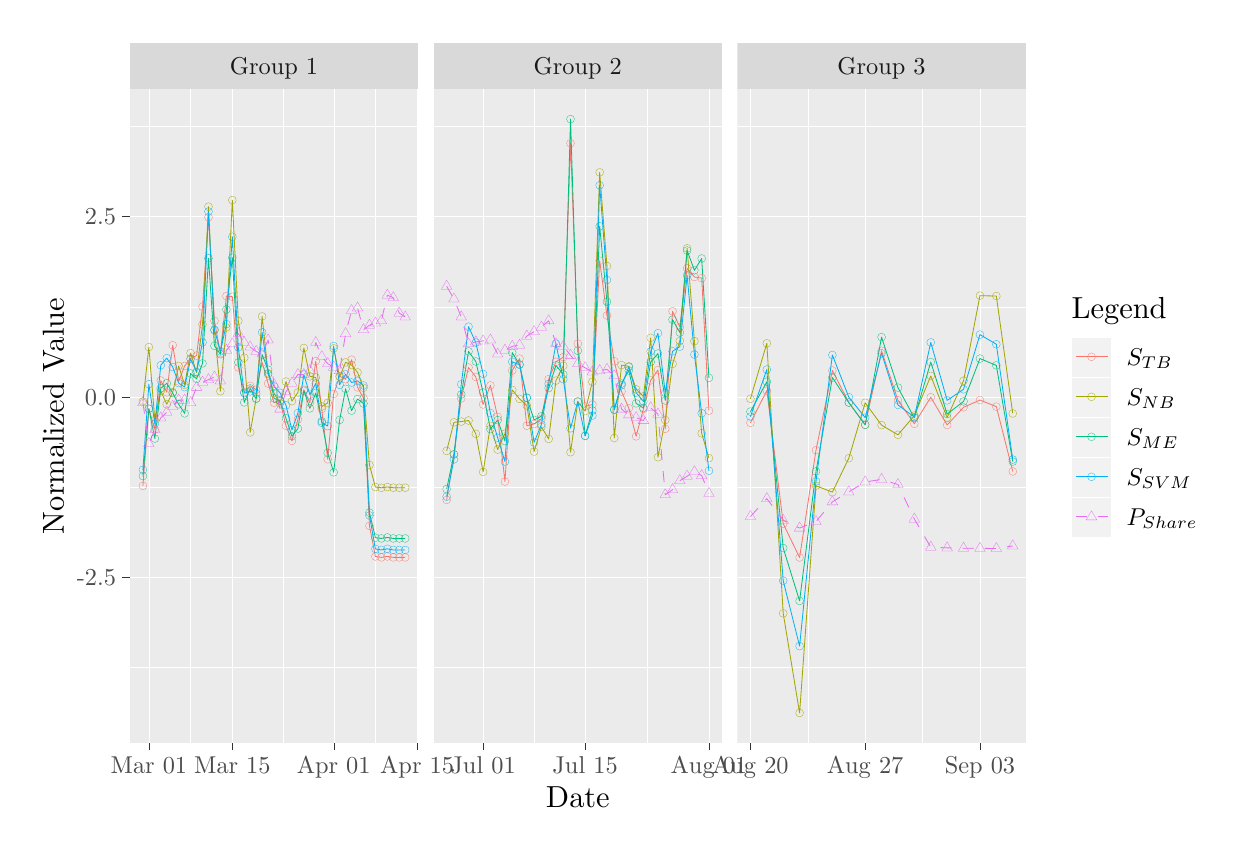
\begin{tikzpicture}[x=1pt,y=1pt]
\definecolor{fillColor}{RGB}{255,255,255}
\path[use as bounding box,fill=fillColor,fill opacity=0.00] (0,0) rectangle (433.62,289.08);
\begin{scope}
\path[clip] (  0.00,  0.00) rectangle (433.62,289.08);
\definecolor{drawColor}{RGB}{255,255,255}
\definecolor{fillColor}{RGB}{255,255,255}

\path[draw=drawColor,line width= 0.1pt,line join=round,line cap=round,fill=fillColor] (  0.00,  0.00) rectangle (433.62,289.08);
\end{scope}
\begin{scope}
\path[clip] ( 36.90, 30.73) rectangle (141.16,266.77);
\definecolor{fillColor}{gray}{0.92}

\path[fill=fillColor] ( 36.90, 30.73) rectangle (141.16,266.77);
\definecolor{drawColor}{RGB}{255,255,255}

\path[draw=drawColor,line width= 0.1pt,line join=round] ( 36.90, 57.88) --
	(141.16, 57.88);

\path[draw=drawColor,line width= 0.1pt,line join=round] ( 36.90,123.08) --
	(141.16,123.08);

\path[draw=drawColor,line width= 0.1pt,line join=round] ( 36.90,188.27) --
	(141.16,188.27);

\path[draw=drawColor,line width= 0.1pt,line join=round] ( 36.90,253.47) --
	(141.16,253.47);

\path[draw=drawColor,line width= 0.1pt,line join=round] ( 58.87, 30.73) --
	( 58.87,266.77);

\path[draw=drawColor,line width= 0.1pt,line join=round] ( 92.26, 30.73) --
	( 92.26,266.77);

\path[draw=drawColor,line width= 0.1pt,line join=round] (125.65, 30.73) --
	(125.65,266.77);

\path[draw=drawColor,line width= 0.1pt,line join=round] ( 36.90, 90.48) --
	(141.16, 90.48);

\path[draw=drawColor,line width= 0.1pt,line join=round] ( 36.90,155.67) --
	(141.16,155.67);

\path[draw=drawColor,line width= 0.1pt,line join=round] ( 36.90,220.87) --
	(141.16,220.87);

\path[draw=drawColor,line width= 0.1pt,line join=round] ( 43.79, 30.73) --
	( 43.79,266.77);

\path[draw=drawColor,line width= 0.1pt,line join=round] ( 73.95, 30.73) --
	( 73.95,266.77);

\path[draw=drawColor,line width= 0.1pt,line join=round] (110.57, 30.73) --
	(110.57,266.77);

\path[draw=drawColor,line width= 0.1pt,line join=round] (140.73, 30.73) --
	(140.73,266.77);
\definecolor{drawColor}{RGB}{248,118,109}

\path[draw=drawColor,line width= 0.3pt,line join=round] ( 41.64,123.51) --
	( 43.79,151.41) --
	( 45.95,143.91) --
	( 48.10,161.57) --
	( 50.26,157.32) --
	( 52.41,174.33) --
	( 54.56,161.28) --
	( 56.72,166.83) --
	( 58.87,169.54) --
	( 61.03,170.59) --
	( 63.18,188.26) --
	( 65.33,220.56) --
	( 67.49,183.15) --
	( 69.64,171.46) --
	( 71.80,192.09) --
	( 73.95,191.87) --
	( 76.11,166.32) --
	( 78.26,157.36) --
	( 80.41,159.65) --
	( 82.57,158.20) --
	( 84.72,168.10) --
	( 86.88,160.50) --
	( 89.03,153.56) --
	( 91.19,154.09) --
	( 93.34,145.21) --
	( 95.49,139.76) --
	( 97.65,147.53) --
	( 99.80,158.27) --
	(101.96,153.51) --
	(104.11,168.56) --
	(106.26,151.32) --
	(108.42,133.10) --
	(110.57,156.69) --
	(112.73,163.13) --
	(114.88,162.06) --
	(117.04,169.11) --
	(119.19,159.12) --
	(121.34,155.22) --
	(123.50,109.05) --
	(125.65, 98.01) --
	(127.81, 97.66) --
	(129.96, 98.01) --
	(132.11, 97.66) --
	(134.27, 97.66) --
	(136.42, 97.66);
\definecolor{drawColor}{RGB}{163,165,0}

\path[draw=drawColor,line width= 0.3pt,line join=round] ( 41.64,154.00) --
	( 43.79,173.67) --
	( 45.95,147.28) --
	( 48.10,157.76) --
	( 50.26,152.99) --
	( 52.41,157.36) --
	( 54.56,166.84) --
	( 56.72,159.99) --
	( 58.87,171.49) --
	( 61.03,164.46) --
	( 63.18,181.86) --
	( 65.33,224.40) --
	( 67.49,179.71) --
	( 69.64,157.70) --
	( 71.80,180.75) --
	( 73.95,226.77) --
	( 76.11,183.14) --
	( 78.26,169.80) --
	( 80.41,142.84) --
	( 82.57,155.09) --
	( 84.72,184.76) --
	( 86.88,164.20) --
	( 89.03,157.00) --
	( 91.19,153.34) --
	( 93.34,161.20) --
	( 95.49,154.14) --
	( 97.65,157.24) --
	( 99.80,173.34) --
	(101.96,163.11) --
	(104.11,162.64) --
	(106.26,152.19) --
	(108.42,153.48) --
	(110.57,173.21) --
	(112.73,162.98) --
	(114.88,168.14) --
	(117.04,167.19) --
	(119.19,164.51) --
	(121.34,158.96) --
	(123.50,131.04) --
	(125.65,123.09) --
	(127.81,122.83) --
	(129.96,123.10) --
	(132.11,122.85) --
	(134.27,122.84) --
	(136.42,122.85);
\definecolor{drawColor}{RGB}{0,191,125}

\path[draw=drawColor,line width= 0.3pt,line join=round] ( 41.64,127.06) --
	( 43.79,151.36) --
	( 45.95,140.61) --
	( 48.10,158.78) --
	( 50.26,160.58) --
	( 52.41,157.06) --
	( 54.56,152.99) --
	( 56.72,149.71) --
	( 58.87,164.10) --
	( 61.03,162.18) --
	( 63.18,167.76) --
	( 65.33,205.76) --
	( 67.49,174.12) --
	( 69.64,171.07) --
	( 71.80,187.26) --
	( 73.95,205.98) --
	( 76.11,168.11) --
	( 78.26,153.67) --
	( 80.41,158.70) --
	( 82.57,154.96) --
	( 84.72,170.94) --
	( 86.88,165.47) --
	( 89.03,155.17) --
	( 91.19,154.31) --
	( 93.34,147.92) --
	( 95.49,141.44) --
	( 97.65,144.21) --
	( 99.80,157.89) --
	(101.96,151.52) --
	(104.11,157.08) --
	(106.26,146.88) --
	(108.42,135.44) --
	(110.57,128.41) --
	(112.73,147.34) --
	(114.88,158.57) --
	(117.04,150.69) --
	(119.19,154.89) --
	(121.34,153.25) --
	(123.50,113.82) --
	(125.65,104.78) --
	(127.81,104.52) --
	(129.96,104.87) --
	(132.11,104.52) --
	(134.27,104.52) --
	(136.42,104.52);
\definecolor{drawColor}{RGB}{0,176,246}

\path[draw=drawColor,line width= 0.3pt,line join=round] ( 41.64,129.31) --
	( 43.79,160.26) --
	( 45.95,145.93) --
	( 48.10,167.10) --
	( 50.26,169.68) --
	( 52.41,166.46) --
	( 54.56,160.64) --
	( 56.72,159.20) --
	( 58.87,169.35) --
	( 61.03,164.70) --
	( 63.18,175.36) --
	( 65.33,222.64) --
	( 67.49,179.93) --
	( 69.64,172.11) --
	( 71.80,181.95) --
	( 73.95,213.53) --
	( 76.11,173.58) --
	( 78.26,157.02) --
	( 80.41,157.66) --
	( 82.57,156.83) --
	( 84.72,178.99) --
	( 86.88,163.89) --
	( 89.03,159.43) --
	( 91.19,157.13) --
	( 93.34,152.62) --
	( 95.49,143.67) --
	( 97.65,149.82) --
	( 99.80,163.76) --
	(101.96,156.48) --
	(104.11,160.56) --
	(106.26,146.32) --
	(108.42,145.10) --
	(110.57,174.05) --
	(112.73,160.04) --
	(114.88,163.81) --
	(117.04,160.85) --
	(119.19,161.46) --
	(121.34,159.79) --
	(123.50,112.83) --
	(125.65,100.72) --
	(127.81,100.37) --
	(129.96,100.77) --
	(132.11,100.36) --
	(134.27,100.36) --
	(136.42,100.36);
\definecolor{drawColor}{RGB}{231,107,243}

\path[draw=drawColor,line width= 0.3pt,dash pattern=on 4pt off 4pt ,line join=round] ( 41.64,153.58) --
	( 43.79,138.79) --
	( 45.95,143.87) --
	( 48.10,148.03) --
	( 50.26,150.11) --
	( 52.41,152.19) --
	( 54.56,154.50) --
	( 56.72,154.50) --
	( 58.87,153.58) --
	( 61.03,159.13) --
	( 63.18,160.98) --
	( 65.33,161.90) --
	( 67.49,162.83) --
	( 69.64,161.44) --
	( 71.80,172.53) --
	( 73.95,174.85) --
	( 76.11,178.54) --
	( 78.26,175.31) --
	( 80.41,173.69) --
	( 82.57,172.07) --
	( 84.72,171.15) --
	( 86.88,176.23) --
	( 89.03,160.05) --
	( 91.19,151.27) --
	( 93.34,157.51) --
	( 95.49,160.63) --
	( 97.65,163.75) --
	( 99.80,163.75) --
	(101.96,165.14) --
	(104.11,175.31) --
	(106.26,170.22) --
	(108.42,167.68) --
	(110.57,166.41) --
	(112.73,165.14) --
	(114.88,178.54) --
	(117.04,186.87) --
	(119.19,187.79) --
	(121.34,179.93) --
	(123.50,181.55) --
	(125.65,182.36) --
	(127.81,183.17) --
	(129.96,192.41) --
	(132.11,191.49) --
	(134.27,185.94) --
	(136.42,184.55);
\definecolor{drawColor}{RGB}{248,118,109}

\path[draw=drawColor,line width= 0.1pt,line join=round,line cap=round] ( 41.64,123.51) circle (  1.43);

\path[draw=drawColor,line width= 0.1pt,line join=round,line cap=round] ( 43.79,151.41) circle (  1.43);

\path[draw=drawColor,line width= 0.1pt,line join=round,line cap=round] ( 45.95,143.91) circle (  1.43);

\path[draw=drawColor,line width= 0.1pt,line join=round,line cap=round] ( 48.10,161.57) circle (  1.43);

\path[draw=drawColor,line width= 0.1pt,line join=round,line cap=round] ( 50.26,157.32) circle (  1.43);

\path[draw=drawColor,line width= 0.1pt,line join=round,line cap=round] ( 52.41,174.33) circle (  1.43);

\path[draw=drawColor,line width= 0.1pt,line join=round,line cap=round] ( 54.56,161.28) circle (  1.43);

\path[draw=drawColor,line width= 0.1pt,line join=round,line cap=round] ( 56.72,166.83) circle (  1.43);

\path[draw=drawColor,line width= 0.1pt,line join=round,line cap=round] ( 58.87,169.54) circle (  1.43);

\path[draw=drawColor,line width= 0.1pt,line join=round,line cap=round] ( 61.03,170.59) circle (  1.43);

\path[draw=drawColor,line width= 0.1pt,line join=round,line cap=round] ( 63.18,188.26) circle (  1.43);

\path[draw=drawColor,line width= 0.1pt,line join=round,line cap=round] ( 65.33,220.56) circle (  1.43);

\path[draw=drawColor,line width= 0.1pt,line join=round,line cap=round] ( 67.49,183.15) circle (  1.43);

\path[draw=drawColor,line width= 0.1pt,line join=round,line cap=round] ( 69.64,171.46) circle (  1.43);

\path[draw=drawColor,line width= 0.1pt,line join=round,line cap=round] ( 71.80,192.09) circle (  1.43);

\path[draw=drawColor,line width= 0.1pt,line join=round,line cap=round] ( 73.95,191.87) circle (  1.43);

\path[draw=drawColor,line width= 0.1pt,line join=round,line cap=round] ( 76.11,166.32) circle (  1.43);

\path[draw=drawColor,line width= 0.1pt,line join=round,line cap=round] ( 78.26,157.36) circle (  1.43);

\path[draw=drawColor,line width= 0.1pt,line join=round,line cap=round] ( 80.41,159.65) circle (  1.43);

\path[draw=drawColor,line width= 0.1pt,line join=round,line cap=round] ( 82.57,158.20) circle (  1.43);

\path[draw=drawColor,line width= 0.1pt,line join=round,line cap=round] ( 84.72,168.10) circle (  1.43);

\path[draw=drawColor,line width= 0.1pt,line join=round,line cap=round] ( 86.88,160.50) circle (  1.43);

\path[draw=drawColor,line width= 0.1pt,line join=round,line cap=round] ( 89.03,153.56) circle (  1.43);

\path[draw=drawColor,line width= 0.1pt,line join=round,line cap=round] ( 91.19,154.09) circle (  1.43);

\path[draw=drawColor,line width= 0.1pt,line join=round,line cap=round] ( 93.34,145.21) circle (  1.43);

\path[draw=drawColor,line width= 0.1pt,line join=round,line cap=round] ( 95.49,139.76) circle (  1.43);

\path[draw=drawColor,line width= 0.1pt,line join=round,line cap=round] ( 97.65,147.53) circle (  1.43);

\path[draw=drawColor,line width= 0.1pt,line join=round,line cap=round] ( 99.80,158.27) circle (  1.43);

\path[draw=drawColor,line width= 0.1pt,line join=round,line cap=round] (101.96,153.51) circle (  1.43);

\path[draw=drawColor,line width= 0.1pt,line join=round,line cap=round] (104.11,168.56) circle (  1.43);

\path[draw=drawColor,line width= 0.1pt,line join=round,line cap=round] (106.26,151.32) circle (  1.43);

\path[draw=drawColor,line width= 0.1pt,line join=round,line cap=round] (108.42,133.10) circle (  1.43);

\path[draw=drawColor,line width= 0.1pt,line join=round,line cap=round] (110.57,156.69) circle (  1.43);

\path[draw=drawColor,line width= 0.1pt,line join=round,line cap=round] (112.73,163.13) circle (  1.43);

\path[draw=drawColor,line width= 0.1pt,line join=round,line cap=round] (114.88,162.06) circle (  1.43);

\path[draw=drawColor,line width= 0.1pt,line join=round,line cap=round] (117.04,169.11) circle (  1.43);

\path[draw=drawColor,line width= 0.1pt,line join=round,line cap=round] (119.19,159.12) circle (  1.43);

\path[draw=drawColor,line width= 0.1pt,line join=round,line cap=round] (121.34,155.22) circle (  1.43);

\path[draw=drawColor,line width= 0.1pt,line join=round,line cap=round] (123.50,109.05) circle (  1.43);

\path[draw=drawColor,line width= 0.1pt,line join=round,line cap=round] (125.65, 98.01) circle (  1.43);

\path[draw=drawColor,line width= 0.1pt,line join=round,line cap=round] (127.81, 97.66) circle (  1.43);

\path[draw=drawColor,line width= 0.1pt,line join=round,line cap=round] (129.96, 98.01) circle (  1.43);

\path[draw=drawColor,line width= 0.1pt,line join=round,line cap=round] (132.11, 97.66) circle (  1.43);

\path[draw=drawColor,line width= 0.1pt,line join=round,line cap=round] (134.27, 97.66) circle (  1.43);

\path[draw=drawColor,line width= 0.1pt,line join=round,line cap=round] (136.42, 97.66) circle (  1.43);
\definecolor{drawColor}{RGB}{163,165,0}

\path[draw=drawColor,line width= 0.1pt,line join=round,line cap=round] ( 41.64,154.00) circle (  1.43);

\path[draw=drawColor,line width= 0.1pt,line join=round,line cap=round] ( 43.79,173.67) circle (  1.43);

\path[draw=drawColor,line width= 0.1pt,line join=round,line cap=round] ( 45.95,147.28) circle (  1.43);

\path[draw=drawColor,line width= 0.1pt,line join=round,line cap=round] ( 48.10,157.76) circle (  1.43);

\path[draw=drawColor,line width= 0.1pt,line join=round,line cap=round] ( 50.26,152.99) circle (  1.43);

\path[draw=drawColor,line width= 0.1pt,line join=round,line cap=round] ( 52.41,157.36) circle (  1.43);

\path[draw=drawColor,line width= 0.1pt,line join=round,line cap=round] ( 54.56,166.84) circle (  1.43);

\path[draw=drawColor,line width= 0.1pt,line join=round,line cap=round] ( 56.72,159.99) circle (  1.43);

\path[draw=drawColor,line width= 0.1pt,line join=round,line cap=round] ( 58.87,171.49) circle (  1.43);

\path[draw=drawColor,line width= 0.1pt,line join=round,line cap=round] ( 61.03,164.46) circle (  1.43);

\path[draw=drawColor,line width= 0.1pt,line join=round,line cap=round] ( 63.18,181.86) circle (  1.43);

\path[draw=drawColor,line width= 0.1pt,line join=round,line cap=round] ( 65.33,224.40) circle (  1.43);

\path[draw=drawColor,line width= 0.1pt,line join=round,line cap=round] ( 67.49,179.71) circle (  1.43);

\path[draw=drawColor,line width= 0.1pt,line join=round,line cap=round] ( 69.64,157.70) circle (  1.43);

\path[draw=drawColor,line width= 0.1pt,line join=round,line cap=round] ( 71.80,180.75) circle (  1.43);

\path[draw=drawColor,line width= 0.1pt,line join=round,line cap=round] ( 73.95,226.77) circle (  1.43);

\path[draw=drawColor,line width= 0.1pt,line join=round,line cap=round] ( 76.11,183.14) circle (  1.43);

\path[draw=drawColor,line width= 0.1pt,line join=round,line cap=round] ( 78.26,169.80) circle (  1.43);

\path[draw=drawColor,line width= 0.1pt,line join=round,line cap=round] ( 80.41,142.84) circle (  1.43);

\path[draw=drawColor,line width= 0.1pt,line join=round,line cap=round] ( 82.57,155.09) circle (  1.43);

\path[draw=drawColor,line width= 0.1pt,line join=round,line cap=round] ( 84.72,184.76) circle (  1.43);

\path[draw=drawColor,line width= 0.1pt,line join=round,line cap=round] ( 86.88,164.20) circle (  1.43);

\path[draw=drawColor,line width= 0.1pt,line join=round,line cap=round] ( 89.03,157.00) circle (  1.43);

\path[draw=drawColor,line width= 0.1pt,line join=round,line cap=round] ( 91.19,153.34) circle (  1.43);

\path[draw=drawColor,line width= 0.1pt,line join=round,line cap=round] ( 93.34,161.20) circle (  1.43);

\path[draw=drawColor,line width= 0.1pt,line join=round,line cap=round] ( 95.49,154.14) circle (  1.43);

\path[draw=drawColor,line width= 0.1pt,line join=round,line cap=round] ( 97.65,157.24) circle (  1.43);

\path[draw=drawColor,line width= 0.1pt,line join=round,line cap=round] ( 99.80,173.34) circle (  1.43);

\path[draw=drawColor,line width= 0.1pt,line join=round,line cap=round] (101.96,163.11) circle (  1.43);

\path[draw=drawColor,line width= 0.1pt,line join=round,line cap=round] (104.11,162.64) circle (  1.43);

\path[draw=drawColor,line width= 0.1pt,line join=round,line cap=round] (106.26,152.19) circle (  1.43);

\path[draw=drawColor,line width= 0.1pt,line join=round,line cap=round] (108.42,153.48) circle (  1.43);

\path[draw=drawColor,line width= 0.1pt,line join=round,line cap=round] (110.57,173.21) circle (  1.43);

\path[draw=drawColor,line width= 0.1pt,line join=round,line cap=round] (112.73,162.98) circle (  1.43);

\path[draw=drawColor,line width= 0.1pt,line join=round,line cap=round] (114.88,168.14) circle (  1.43);

\path[draw=drawColor,line width= 0.1pt,line join=round,line cap=round] (117.04,167.19) circle (  1.43);

\path[draw=drawColor,line width= 0.1pt,line join=round,line cap=round] (119.19,164.51) circle (  1.43);

\path[draw=drawColor,line width= 0.1pt,line join=round,line cap=round] (121.34,158.96) circle (  1.43);

\path[draw=drawColor,line width= 0.1pt,line join=round,line cap=round] (123.50,131.04) circle (  1.43);

\path[draw=drawColor,line width= 0.1pt,line join=round,line cap=round] (125.65,123.09) circle (  1.43);

\path[draw=drawColor,line width= 0.1pt,line join=round,line cap=round] (127.81,122.83) circle (  1.43);

\path[draw=drawColor,line width= 0.1pt,line join=round,line cap=round] (129.96,123.10) circle (  1.43);

\path[draw=drawColor,line width= 0.1pt,line join=round,line cap=round] (132.11,122.85) circle (  1.43);

\path[draw=drawColor,line width= 0.1pt,line join=round,line cap=round] (134.27,122.84) circle (  1.43);

\path[draw=drawColor,line width= 0.1pt,line join=round,line cap=round] (136.42,122.85) circle (  1.43);
\definecolor{drawColor}{RGB}{0,191,125}

\path[draw=drawColor,line width= 0.1pt,line join=round,line cap=round] ( 41.64,127.06) circle (  1.43);

\path[draw=drawColor,line width= 0.1pt,line join=round,line cap=round] ( 43.79,151.36) circle (  1.43);

\path[draw=drawColor,line width= 0.1pt,line join=round,line cap=round] ( 45.95,140.61) circle (  1.43);

\path[draw=drawColor,line width= 0.1pt,line join=round,line cap=round] ( 48.10,158.78) circle (  1.43);

\path[draw=drawColor,line width= 0.1pt,line join=round,line cap=round] ( 50.26,160.58) circle (  1.43);

\path[draw=drawColor,line width= 0.1pt,line join=round,line cap=round] ( 52.41,157.06) circle (  1.43);

\path[draw=drawColor,line width= 0.1pt,line join=round,line cap=round] ( 54.56,152.99) circle (  1.43);

\path[draw=drawColor,line width= 0.1pt,line join=round,line cap=round] ( 56.72,149.71) circle (  1.43);

\path[draw=drawColor,line width= 0.1pt,line join=round,line cap=round] ( 58.87,164.10) circle (  1.43);

\path[draw=drawColor,line width= 0.1pt,line join=round,line cap=round] ( 61.03,162.18) circle (  1.43);

\path[draw=drawColor,line width= 0.1pt,line join=round,line cap=round] ( 63.18,167.76) circle (  1.43);

\path[draw=drawColor,line width= 0.1pt,line join=round,line cap=round] ( 65.33,205.76) circle (  1.43);

\path[draw=drawColor,line width= 0.1pt,line join=round,line cap=round] ( 67.49,174.12) circle (  1.43);

\path[draw=drawColor,line width= 0.1pt,line join=round,line cap=round] ( 69.64,171.07) circle (  1.43);

\path[draw=drawColor,line width= 0.1pt,line join=round,line cap=round] ( 71.80,187.26) circle (  1.43);

\path[draw=drawColor,line width= 0.1pt,line join=round,line cap=round] ( 73.95,205.98) circle (  1.43);

\path[draw=drawColor,line width= 0.1pt,line join=round,line cap=round] ( 76.11,168.11) circle (  1.43);

\path[draw=drawColor,line width= 0.1pt,line join=round,line cap=round] ( 78.26,153.67) circle (  1.43);

\path[draw=drawColor,line width= 0.1pt,line join=round,line cap=round] ( 80.41,158.70) circle (  1.43);

\path[draw=drawColor,line width= 0.1pt,line join=round,line cap=round] ( 82.57,154.96) circle (  1.43);

\path[draw=drawColor,line width= 0.1pt,line join=round,line cap=round] ( 84.72,170.94) circle (  1.43);

\path[draw=drawColor,line width= 0.1pt,line join=round,line cap=round] ( 86.88,165.47) circle (  1.43);

\path[draw=drawColor,line width= 0.1pt,line join=round,line cap=round] ( 89.03,155.17) circle (  1.43);

\path[draw=drawColor,line width= 0.1pt,line join=round,line cap=round] ( 91.19,154.31) circle (  1.43);

\path[draw=drawColor,line width= 0.1pt,line join=round,line cap=round] ( 93.34,147.92) circle (  1.43);

\path[draw=drawColor,line width= 0.1pt,line join=round,line cap=round] ( 95.49,141.44) circle (  1.43);

\path[draw=drawColor,line width= 0.1pt,line join=round,line cap=round] ( 97.65,144.21) circle (  1.43);

\path[draw=drawColor,line width= 0.1pt,line join=round,line cap=round] ( 99.80,157.89) circle (  1.43);

\path[draw=drawColor,line width= 0.1pt,line join=round,line cap=round] (101.96,151.52) circle (  1.43);

\path[draw=drawColor,line width= 0.1pt,line join=round,line cap=round] (104.11,157.08) circle (  1.43);

\path[draw=drawColor,line width= 0.1pt,line join=round,line cap=round] (106.26,146.88) circle (  1.43);

\path[draw=drawColor,line width= 0.1pt,line join=round,line cap=round] (108.42,135.44) circle (  1.43);

\path[draw=drawColor,line width= 0.1pt,line join=round,line cap=round] (110.57,128.41) circle (  1.43);

\path[draw=drawColor,line width= 0.1pt,line join=round,line cap=round] (112.73,147.34) circle (  1.43);

\path[draw=drawColor,line width= 0.1pt,line join=round,line cap=round] (114.88,158.57) circle (  1.43);

\path[draw=drawColor,line width= 0.1pt,line join=round,line cap=round] (117.04,150.69) circle (  1.43);

\path[draw=drawColor,line width= 0.1pt,line join=round,line cap=round] (119.19,154.89) circle (  1.43);

\path[draw=drawColor,line width= 0.1pt,line join=round,line cap=round] (121.34,153.25) circle (  1.43);

\path[draw=drawColor,line width= 0.1pt,line join=round,line cap=round] (123.50,113.82) circle (  1.43);

\path[draw=drawColor,line width= 0.1pt,line join=round,line cap=round] (125.65,104.78) circle (  1.43);

\path[draw=drawColor,line width= 0.1pt,line join=round,line cap=round] (127.81,104.52) circle (  1.43);

\path[draw=drawColor,line width= 0.1pt,line join=round,line cap=round] (129.96,104.87) circle (  1.43);

\path[draw=drawColor,line width= 0.1pt,line join=round,line cap=round] (132.11,104.52) circle (  1.43);

\path[draw=drawColor,line width= 0.1pt,line join=round,line cap=round] (134.27,104.52) circle (  1.43);

\path[draw=drawColor,line width= 0.1pt,line join=round,line cap=round] (136.42,104.52) circle (  1.43);
\definecolor{drawColor}{RGB}{0,176,246}

\path[draw=drawColor,line width= 0.1pt,line join=round,line cap=round] ( 41.64,129.31) circle (  1.43);

\path[draw=drawColor,line width= 0.1pt,line join=round,line cap=round] ( 43.79,160.26) circle (  1.43);

\path[draw=drawColor,line width= 0.1pt,line join=round,line cap=round] ( 45.95,145.93) circle (  1.43);

\path[draw=drawColor,line width= 0.1pt,line join=round,line cap=round] ( 48.10,167.10) circle (  1.43);

\path[draw=drawColor,line width= 0.1pt,line join=round,line cap=round] ( 50.26,169.68) circle (  1.43);

\path[draw=drawColor,line width= 0.1pt,line join=round,line cap=round] ( 52.41,166.46) circle (  1.43);

\path[draw=drawColor,line width= 0.1pt,line join=round,line cap=round] ( 54.56,160.64) circle (  1.43);

\path[draw=drawColor,line width= 0.1pt,line join=round,line cap=round] ( 56.72,159.20) circle (  1.43);

\path[draw=drawColor,line width= 0.1pt,line join=round,line cap=round] ( 58.87,169.35) circle (  1.43);

\path[draw=drawColor,line width= 0.1pt,line join=round,line cap=round] ( 61.03,164.70) circle (  1.43);

\path[draw=drawColor,line width= 0.1pt,line join=round,line cap=round] ( 63.18,175.36) circle (  1.43);

\path[draw=drawColor,line width= 0.1pt,line join=round,line cap=round] ( 65.33,222.64) circle (  1.43);

\path[draw=drawColor,line width= 0.1pt,line join=round,line cap=round] ( 67.49,179.93) circle (  1.43);

\path[draw=drawColor,line width= 0.1pt,line join=round,line cap=round] ( 69.64,172.11) circle (  1.43);

\path[draw=drawColor,line width= 0.1pt,line join=round,line cap=round] ( 71.80,181.95) circle (  1.43);

\path[draw=drawColor,line width= 0.1pt,line join=round,line cap=round] ( 73.95,213.53) circle (  1.43);

\path[draw=drawColor,line width= 0.1pt,line join=round,line cap=round] ( 76.11,173.58) circle (  1.43);

\path[draw=drawColor,line width= 0.1pt,line join=round,line cap=round] ( 78.26,157.02) circle (  1.43);

\path[draw=drawColor,line width= 0.1pt,line join=round,line cap=round] ( 80.41,157.66) circle (  1.43);

\path[draw=drawColor,line width= 0.1pt,line join=round,line cap=round] ( 82.57,156.83) circle (  1.43);

\path[draw=drawColor,line width= 0.1pt,line join=round,line cap=round] ( 84.72,178.99) circle (  1.43);

\path[draw=drawColor,line width= 0.1pt,line join=round,line cap=round] ( 86.88,163.89) circle (  1.43);

\path[draw=drawColor,line width= 0.1pt,line join=round,line cap=round] ( 89.03,159.43) circle (  1.43);

\path[draw=drawColor,line width= 0.1pt,line join=round,line cap=round] ( 91.19,157.13) circle (  1.43);

\path[draw=drawColor,line width= 0.1pt,line join=round,line cap=round] ( 93.34,152.62) circle (  1.43);

\path[draw=drawColor,line width= 0.1pt,line join=round,line cap=round] ( 95.49,143.67) circle (  1.43);

\path[draw=drawColor,line width= 0.1pt,line join=round,line cap=round] ( 97.65,149.82) circle (  1.43);

\path[draw=drawColor,line width= 0.1pt,line join=round,line cap=round] ( 99.80,163.76) circle (  1.43);

\path[draw=drawColor,line width= 0.1pt,line join=round,line cap=round] (101.96,156.48) circle (  1.43);

\path[draw=drawColor,line width= 0.1pt,line join=round,line cap=round] (104.11,160.56) circle (  1.43);

\path[draw=drawColor,line width= 0.1pt,line join=round,line cap=round] (106.26,146.32) circle (  1.43);

\path[draw=drawColor,line width= 0.1pt,line join=round,line cap=round] (108.42,145.10) circle (  1.43);

\path[draw=drawColor,line width= 0.1pt,line join=round,line cap=round] (110.57,174.05) circle (  1.43);

\path[draw=drawColor,line width= 0.1pt,line join=round,line cap=round] (112.73,160.04) circle (  1.43);

\path[draw=drawColor,line width= 0.1pt,line join=round,line cap=round] (114.88,163.81) circle (  1.43);

\path[draw=drawColor,line width= 0.1pt,line join=round,line cap=round] (117.04,160.85) circle (  1.43);

\path[draw=drawColor,line width= 0.1pt,line join=round,line cap=round] (119.19,161.46) circle (  1.43);

\path[draw=drawColor,line width= 0.1pt,line join=round,line cap=round] (121.34,159.79) circle (  1.43);

\path[draw=drawColor,line width= 0.1pt,line join=round,line cap=round] (123.50,112.83) circle (  1.43);

\path[draw=drawColor,line width= 0.1pt,line join=round,line cap=round] (125.65,100.72) circle (  1.43);

\path[draw=drawColor,line width= 0.1pt,line join=round,line cap=round] (127.81,100.37) circle (  1.43);

\path[draw=drawColor,line width= 0.1pt,line join=round,line cap=round] (129.96,100.77) circle (  1.43);

\path[draw=drawColor,line width= 0.1pt,line join=round,line cap=round] (132.11,100.36) circle (  1.43);

\path[draw=drawColor,line width= 0.1pt,line join=round,line cap=round] (134.27,100.36) circle (  1.43);

\path[draw=drawColor,line width= 0.1pt,line join=round,line cap=round] (136.42,100.36) circle (  1.43);
\definecolor{drawColor}{RGB}{231,107,243}

\path[draw=drawColor,line width= 0.1pt,line join=round,line cap=round] ( 41.64,155.80) --
	( 43.56,152.47) --
	( 39.72,152.47) --
	( 41.64,155.80);

\path[draw=drawColor,line width= 0.1pt,line join=round,line cap=round] ( 43.79,141.00) --
	( 45.71,137.68) --
	( 41.87,137.68) --
	( 43.79,141.00);

\path[draw=drawColor,line width= 0.1pt,line join=round,line cap=round] ( 45.95,146.09) --
	( 47.87,142.76) --
	( 44.03,142.76) --
	( 45.95,146.09);

\path[draw=drawColor,line width= 0.1pt,line join=round,line cap=round] ( 48.10,150.25) --
	( 50.02,146.92) --
	( 46.18,146.92) --
	( 48.10,150.25);

\path[draw=drawColor,line width= 0.1pt,line join=round,line cap=round] ( 50.26,152.33) --
	( 52.18,149.00) --
	( 48.33,149.00) --
	( 50.26,152.33);

\path[draw=drawColor,line width= 0.1pt,line join=round,line cap=round] ( 52.41,154.41) --
	( 54.33,151.08) --
	( 50.49,151.08) --
	( 52.41,154.41);

\path[draw=drawColor,line width= 0.1pt,line join=round,line cap=round] ( 54.56,156.72) --
	( 56.49,153.40) --
	( 52.64,153.40) --
	( 54.56,156.72);

\path[draw=drawColor,line width= 0.1pt,line join=round,line cap=round] ( 56.72,156.72) --
	( 58.64,153.40) --
	( 54.80,153.40) --
	( 56.72,156.72);

\path[draw=drawColor,line width= 0.1pt,line join=round,line cap=round] ( 58.87,155.80) --
	( 60.79,152.47) --
	( 56.95,152.47) --
	( 58.87,155.80);

\path[draw=drawColor,line width= 0.1pt,line join=round,line cap=round] ( 61.03,161.35) --
	( 62.95,158.02) --
	( 59.11,158.02) --
	( 61.03,161.35);

\path[draw=drawColor,line width= 0.1pt,line join=round,line cap=round] ( 63.18,163.20) --
	( 65.10,159.87) --
	( 61.26,159.87) --
	( 63.18,163.20);

\path[draw=drawColor,line width= 0.1pt,line join=round,line cap=round] ( 65.33,164.12) --
	( 67.26,160.79) --
	( 63.41,160.79) --
	( 65.33,164.12);

\path[draw=drawColor,line width= 0.1pt,line join=round,line cap=round] ( 67.49,165.04) --
	( 69.41,161.72) --
	( 65.57,161.72) --
	( 67.49,165.04);

\path[draw=drawColor,line width= 0.1pt,line join=round,line cap=round] ( 69.64,163.66) --
	( 71.56,160.33) --
	( 67.72,160.33) --
	( 69.64,163.66);

\path[draw=drawColor,line width= 0.1pt,line join=round,line cap=round] ( 71.80,174.75) --
	( 73.72,171.42) --
	( 69.88,171.42) --
	( 71.80,174.75);

\path[draw=drawColor,line width= 0.1pt,line join=round,line cap=round] ( 73.95,177.06) --
	( 75.87,173.74) --
	( 72.03,173.74) --
	( 73.95,177.06);

\path[draw=drawColor,line width= 0.1pt,line join=round,line cap=round] ( 76.11,180.76) --
	( 78.03,177.43) --
	( 74.18,177.43) --
	( 76.11,180.76);

\path[draw=drawColor,line width= 0.1pt,line join=round,line cap=round] ( 78.26,177.53) --
	( 80.18,174.20) --
	( 76.34,174.20) --
	( 78.26,177.53);

\path[draw=drawColor,line width= 0.1pt,line join=round,line cap=round] ( 80.41,175.91) --
	( 82.34,172.58) --
	( 78.49,172.58) --
	( 80.41,175.91);

\path[draw=drawColor,line width= 0.1pt,line join=round,line cap=round] ( 82.57,174.29) --
	( 84.49,170.96) --
	( 80.65,170.96) --
	( 82.57,174.29);

\path[draw=drawColor,line width= 0.1pt,line join=round,line cap=round] ( 84.72,173.37) --
	( 86.64,170.04) --
	( 82.80,170.04) --
	( 84.72,173.37);

\path[draw=drawColor,line width= 0.1pt,line join=round,line cap=round] ( 86.88,178.45) --
	( 88.80,175.12) --
	( 84.96,175.12) --
	( 86.88,178.45);

\path[draw=drawColor,line width= 0.1pt,line join=round,line cap=round] ( 89.03,162.27) --
	( 90.95,158.94) --
	( 87.11,158.94) --
	( 89.03,162.27);

\path[draw=drawColor,line width= 0.1pt,line join=round,line cap=round] ( 91.19,153.49) --
	( 93.11,150.16) --
	( 89.26,150.16) --
	( 91.19,153.49);

\path[draw=drawColor,line width= 0.1pt,line join=round,line cap=round] ( 93.34,159.73) --
	( 95.26,156.40) --
	( 91.42,156.40) --
	( 93.34,159.73);

\path[draw=drawColor,line width= 0.1pt,line join=round,line cap=round] ( 95.49,162.85) --
	( 97.41,159.52) --
	( 93.57,159.52) --
	( 95.49,162.85);

\path[draw=drawColor,line width= 0.1pt,line join=round,line cap=round] ( 97.65,165.97) --
	( 99.57,162.64) --
	( 95.73,162.64) --
	( 97.65,165.97);

\path[draw=drawColor,line width= 0.1pt,line join=round,line cap=round] ( 99.80,165.97) --
	(101.72,162.64) --
	( 97.88,162.64) --
	( 99.80,165.97);

\path[draw=drawColor,line width= 0.1pt,line join=round,line cap=round] (101.96,167.36) --
	(103.88,164.03) --
	(100.03,164.03) --
	(101.96,167.36);

\path[draw=drawColor,line width= 0.1pt,line join=round,line cap=round] (104.11,177.53) --
	(106.03,174.20) --
	(102.19,174.20) --
	(104.11,177.53);

\path[draw=drawColor,line width= 0.1pt,line join=round,line cap=round] (106.26,172.44) --
	(108.19,169.11) --
	(104.34,169.11) --
	(106.26,172.44);

\path[draw=drawColor,line width= 0.1pt,line join=round,line cap=round] (108.42,169.90) --
	(110.34,166.57) --
	(106.50,166.57) --
	(108.42,169.90);

\path[draw=drawColor,line width= 0.1pt,line join=round,line cap=round] (110.57,168.63) --
	(112.49,165.30) --
	(108.65,165.30) --
	(110.57,168.63);

\path[draw=drawColor,line width= 0.1pt,line join=round,line cap=round] (112.73,167.36) --
	(114.65,164.03) --
	(110.81,164.03) --
	(112.73,167.36);

\path[draw=drawColor,line width= 0.1pt,line join=round,line cap=round] (114.88,180.76) --
	(116.80,177.43) --
	(112.96,177.43) --
	(114.88,180.76);

\path[draw=drawColor,line width= 0.1pt,line join=round,line cap=round] (117.04,189.08) --
	(118.96,185.76) --
	(115.11,185.76) --
	(117.04,189.08);

\path[draw=drawColor,line width= 0.1pt,line join=round,line cap=round] (119.19,190.01) --
	(121.11,186.68) --
	(117.27,186.68) --
	(119.19,190.01);

\path[draw=drawColor,line width= 0.1pt,line join=round,line cap=round] (121.34,182.15) --
	(123.26,178.82) --
	(119.42,178.82) --
	(121.34,182.15);

\path[draw=drawColor,line width= 0.1pt,line join=round,line cap=round] (123.50,183.77) --
	(125.42,180.44) --
	(121.58,180.44) --
	(123.50,183.77);

\path[draw=drawColor,line width= 0.1pt,line join=round,line cap=round] (125.65,184.58) --
	(127.57,181.25) --
	(123.73,181.25) --
	(125.65,184.58);

\path[draw=drawColor,line width= 0.1pt,line join=round,line cap=round] (127.81,185.39) --
	(129.73,182.06) --
	(125.88,182.06) --
	(127.81,185.39);

\path[draw=drawColor,line width= 0.1pt,line join=round,line cap=round] (129.96,194.63) --
	(131.88,191.30) --
	(128.04,191.30) --
	(129.96,194.63);

\path[draw=drawColor,line width= 0.1pt,line join=round,line cap=round] (132.11,193.71) --
	(134.04,190.38) --
	(130.19,190.38) --
	(132.11,193.71);

\path[draw=drawColor,line width= 0.1pt,line join=round,line cap=round] (134.27,188.16) --
	(136.19,184.83) --
	(132.35,184.83) --
	(134.27,188.16);

\path[draw=drawColor,line width= 0.1pt,line join=round,line cap=round] (136.42,186.77) --
	(138.34,183.44) --
	(134.50,183.44) --
	(136.42,186.77);
\end{scope}
\begin{scope}
\path[clip] (146.66, 30.73) rectangle (250.92,266.77);
\definecolor{fillColor}{gray}{0.92}

\path[fill=fillColor] (146.66, 30.73) rectangle (250.92,266.77);
\definecolor{drawColor}{RGB}{255,255,255}

\path[draw=drawColor,line width= 0.1pt,line join=round] (146.66, 57.88) --
	(250.92, 57.88);

\path[draw=drawColor,line width= 0.1pt,line join=round] (146.66,123.08) --
	(250.92,123.08);

\path[draw=drawColor,line width= 0.1pt,line join=round] (146.66,188.27) --
	(250.92,188.27);

\path[draw=drawColor,line width= 0.1pt,line join=round] (146.66,253.47) --
	(250.92,253.47);

\path[draw=drawColor,line width= 0.1pt,line join=round] (183.00, 30.73) --
	(183.00,266.77);

\path[draw=drawColor,line width= 0.1pt,line join=round] (223.81, 30.73) --
	(223.81,266.77);

\path[draw=drawColor,line width= 0.1pt,line join=round] (146.66, 90.48) --
	(250.92, 90.48);

\path[draw=drawColor,line width= 0.1pt,line join=round] (146.66,155.67) --
	(250.92,155.67);

\path[draw=drawColor,line width= 0.1pt,line join=round] (146.66,220.87) --
	(250.92,220.87);

\path[draw=drawColor,line width= 0.1pt,line join=round] (164.57, 30.73) --
	(164.57,266.77);

\path[draw=drawColor,line width= 0.1pt,line join=round] (201.43, 30.73) --
	(201.43,266.77);

\path[draw=drawColor,line width= 0.1pt,line join=round] (246.18, 30.73) --
	(246.18,266.77);
\definecolor{drawColor}{RGB}{248,118,109}

\path[draw=drawColor,line width= 0.3pt,line join=round] (151.40,118.43) --
	(154.03,134.88) --
	(156.67,155.12) --
	(159.30,166.28) --
	(161.93,162.86) --
	(164.57,152.93) --
	(167.20,159.82) --
	(169.83,148.45) --
	(172.46,125.08) --
	(175.10,165.21) --
	(177.73,169.49) --
	(180.36,145.24) --
	(183.00,145.87) --
	(185.63,147.74) --
	(188.26,162.06) --
	(190.89,168.35) --
	(193.53,170.03) --
	(196.16,247.31) --
	(198.79,174.90) --
	(201.43,152.22) --
	(204.06,152.89) --
	(206.69,204.87) --
	(209.32,185.09) --
	(211.96,168.54) --
	(214.59,157.61) --
	(217.22,151.59) --
	(219.86,141.42) --
	(222.49,151.30) --
	(225.12,161.64) --
	(227.75,165.37) --
	(230.39,144.11) --
	(233.02,186.59) --
	(235.65,180.92) --
	(238.29,202.13) --
	(240.92,198.99) --
	(243.55,198.57) --
	(246.18,150.67);
\definecolor{drawColor}{RGB}{163,165,0}

\path[draw=drawColor,line width= 0.3pt,line join=round] (151.40,136.14) --
	(154.03,146.46) --
	(156.67,146.74) --
	(159.30,147.13) --
	(161.93,142.33) --
	(164.57,128.54) --
	(167.20,145.20) --
	(169.83,136.63) --
	(172.46,142.39) --
	(175.10,158.17) --
	(177.73,154.95) --
	(180.36,152.58) --
	(183.00,135.88) --
	(185.63,144.84) --
	(188.26,140.48) --
	(190.89,161.54) --
	(193.53,166.91) --
	(196.16,135.68) --
	(198.79,153.90) --
	(201.43,150.53) --
	(204.06,161.12) --
	(206.69,236.79) --
	(209.32,202.95) --
	(211.96,140.80) --
	(214.59,167.15) --
	(217.22,166.71) --
	(219.86,158.40) --
	(222.49,155.85) --
	(225.12,176.99) --
	(227.75,133.88) --
	(230.39,147.31) --
	(233.02,167.57) --
	(235.65,175.87) --
	(238.29,209.36) --
	(240.92,175.81) --
	(243.55,142.53) --
	(246.18,133.53);
\definecolor{drawColor}{RGB}{0,191,125}

\path[draw=drawColor,line width= 0.3pt,line join=round] (151.40,122.37) --
	(154.03,134.90) --
	(156.67,156.54) --
	(159.30,172.10) --
	(161.93,168.45) --
	(164.57,157.25) --
	(167.20,144.03) --
	(169.83,147.28) --
	(172.46,139.70) --
	(175.10,171.66) --
	(177.73,167.40) --
	(180.36,155.32) --
	(183.00,147.34) --
	(185.63,148.67) --
	(188.26,158.85) --
	(190.89,167.04) --
	(193.53,163.81) --
	(196.16,256.04) --
	(198.79,172.34) --
	(201.43,141.64) --
	(204.06,150.74) --
	(206.69,217.31) --
	(209.32,190.06) --
	(211.96,151.13) --
	(214.59,160.45) --
	(217.22,165.21) --
	(219.86,153.31) --
	(222.49,151.66) --
	(225.12,168.24) --
	(227.75,171.33) --
	(230.39,154.37) --
	(233.02,183.58) --
	(235.65,178.92) --
	(238.29,208.55) --
	(240.92,201.39) --
	(243.55,205.66) --
	(246.18,162.52);
\definecolor{drawColor}{RGB}{0,176,246}

\path[draw=drawColor,line width= 0.3pt,line join=round] (151.40,119.60) --
	(154.03,133.06) --
	(156.67,160.18) --
	(159.30,181.04) --
	(161.93,175.30) --
	(164.57,163.98) --
	(167.20,149.83) --
	(169.83,140.87) --
	(172.46,132.29) --
	(175.10,168.33) --
	(177.73,167.25) --
	(180.36,155.38) --
	(183.00,139.22) --
	(185.63,145.68) --
	(188.26,160.34) --
	(190.89,174.89) --
	(193.53,162.06) --
	(196.16,144.33) --
	(198.79,154.03) --
	(201.43,141.51) --
	(204.06,148.89) --
	(206.69,232.12) --
	(209.32,197.91) --
	(211.96,150.94) --
	(214.59,159.90) --
	(217.22,166.47) --
	(219.86,157.23) --
	(222.49,154.04) --
	(225.12,172.08) --
	(227.75,178.68) --
	(230.39,157.17) --
	(233.02,172.14) --
	(235.65,173.81) --
	(238.29,199.55) --
	(240.92,170.96) --
	(243.55,149.76) --
	(246.18,128.96);
\definecolor{drawColor}{RGB}{231,107,243}

\path[draw=drawColor,line width= 0.3pt,dash pattern=on 4pt off 4pt ,line join=round] (151.40,195.65) --
	(154.03,191.03) --
	(156.67,184.55) --
	(159.30,174.85) --
	(161.93,175.54) --
	(164.57,175.89) --
	(167.20,176.23) --
	(169.83,171.15) --
	(172.46,172.53) --
	(175.10,173.92) --
	(177.73,174.38) --
	(180.36,177.62) --
	(183.00,179.24) --
	(185.63,180.86) --
	(188.26,183.17) --
	(190.89,174.85) --
	(193.53,173.92) --
	(196.16,170.68) --
	(198.79,167.68) --
	(201.43,166.18) --
	(204.06,164.67) --
	(206.69,165.14) --
	(209.32,165.60) --
	(211.96,163.29) --
	(214.59,151.27) --
	(217.22,149.19) --
	(219.86,148.15) --
	(222.49,147.11) --
	(225.12,151.73) --
	(227.75,149.42) --
	(230.39,120.29) --
	(233.02,122.14) --
	(235.65,125.38) --
	(238.29,127.00) --
	(240.92,128.62) --
	(243.55,127.23) --
	(246.18,120.76);
\definecolor{drawColor}{RGB}{248,118,109}

\path[draw=drawColor,line width= 0.1pt,line join=round,line cap=round] (151.40,118.43) circle (  1.43);

\path[draw=drawColor,line width= 0.1pt,line join=round,line cap=round] (154.03,134.88) circle (  1.43);

\path[draw=drawColor,line width= 0.1pt,line join=round,line cap=round] (156.67,155.12) circle (  1.43);

\path[draw=drawColor,line width= 0.1pt,line join=round,line cap=round] (159.30,166.28) circle (  1.43);

\path[draw=drawColor,line width= 0.1pt,line join=round,line cap=round] (161.93,162.86) circle (  1.43);

\path[draw=drawColor,line width= 0.1pt,line join=round,line cap=round] (164.57,152.93) circle (  1.43);

\path[draw=drawColor,line width= 0.1pt,line join=round,line cap=round] (167.20,159.82) circle (  1.43);

\path[draw=drawColor,line width= 0.1pt,line join=round,line cap=round] (169.83,148.45) circle (  1.43);

\path[draw=drawColor,line width= 0.1pt,line join=round,line cap=round] (172.46,125.08) circle (  1.43);

\path[draw=drawColor,line width= 0.1pt,line join=round,line cap=round] (175.10,165.21) circle (  1.43);

\path[draw=drawColor,line width= 0.1pt,line join=round,line cap=round] (177.73,169.49) circle (  1.43);

\path[draw=drawColor,line width= 0.1pt,line join=round,line cap=round] (180.36,145.24) circle (  1.43);

\path[draw=drawColor,line width= 0.1pt,line join=round,line cap=round] (183.00,145.87) circle (  1.43);

\path[draw=drawColor,line width= 0.1pt,line join=round,line cap=round] (185.63,147.74) circle (  1.43);

\path[draw=drawColor,line width= 0.1pt,line join=round,line cap=round] (188.26,162.06) circle (  1.43);

\path[draw=drawColor,line width= 0.1pt,line join=round,line cap=round] (190.89,168.35) circle (  1.43);

\path[draw=drawColor,line width= 0.1pt,line join=round,line cap=round] (193.53,170.03) circle (  1.43);

\path[draw=drawColor,line width= 0.1pt,line join=round,line cap=round] (196.16,247.31) circle (  1.43);

\path[draw=drawColor,line width= 0.1pt,line join=round,line cap=round] (198.79,174.90) circle (  1.43);

\path[draw=drawColor,line width= 0.1pt,line join=round,line cap=round] (201.43,152.22) circle (  1.43);

\path[draw=drawColor,line width= 0.1pt,line join=round,line cap=round] (204.06,152.89) circle (  1.43);

\path[draw=drawColor,line width= 0.1pt,line join=round,line cap=round] (206.69,204.87) circle (  1.43);

\path[draw=drawColor,line width= 0.1pt,line join=round,line cap=round] (209.32,185.09) circle (  1.43);

\path[draw=drawColor,line width= 0.1pt,line join=round,line cap=round] (211.96,168.54) circle (  1.43);

\path[draw=drawColor,line width= 0.1pt,line join=round,line cap=round] (214.59,157.61) circle (  1.43);

\path[draw=drawColor,line width= 0.1pt,line join=round,line cap=round] (217.22,151.59) circle (  1.43);

\path[draw=drawColor,line width= 0.1pt,line join=round,line cap=round] (219.86,141.42) circle (  1.43);

\path[draw=drawColor,line width= 0.1pt,line join=round,line cap=round] (222.49,151.30) circle (  1.43);

\path[draw=drawColor,line width= 0.1pt,line join=round,line cap=round] (225.12,161.64) circle (  1.43);

\path[draw=drawColor,line width= 0.1pt,line join=round,line cap=round] (227.75,165.37) circle (  1.43);

\path[draw=drawColor,line width= 0.1pt,line join=round,line cap=round] (230.39,144.11) circle (  1.43);

\path[draw=drawColor,line width= 0.1pt,line join=round,line cap=round] (233.02,186.59) circle (  1.43);

\path[draw=drawColor,line width= 0.1pt,line join=round,line cap=round] (235.65,180.92) circle (  1.43);

\path[draw=drawColor,line width= 0.1pt,line join=round,line cap=round] (238.29,202.13) circle (  1.43);

\path[draw=drawColor,line width= 0.1pt,line join=round,line cap=round] (240.92,198.99) circle (  1.43);

\path[draw=drawColor,line width= 0.1pt,line join=round,line cap=round] (243.55,198.57) circle (  1.43);

\path[draw=drawColor,line width= 0.1pt,line join=round,line cap=round] (246.18,150.67) circle (  1.43);
\definecolor{drawColor}{RGB}{163,165,0}

\path[draw=drawColor,line width= 0.1pt,line join=round,line cap=round] (151.40,136.14) circle (  1.43);

\path[draw=drawColor,line width= 0.1pt,line join=round,line cap=round] (154.03,146.46) circle (  1.43);

\path[draw=drawColor,line width= 0.1pt,line join=round,line cap=round] (156.67,146.74) circle (  1.43);

\path[draw=drawColor,line width= 0.1pt,line join=round,line cap=round] (159.30,147.13) circle (  1.43);

\path[draw=drawColor,line width= 0.1pt,line join=round,line cap=round] (161.93,142.33) circle (  1.43);

\path[draw=drawColor,line width= 0.1pt,line join=round,line cap=round] (164.57,128.54) circle (  1.43);

\path[draw=drawColor,line width= 0.1pt,line join=round,line cap=round] (167.20,145.20) circle (  1.43);

\path[draw=drawColor,line width= 0.1pt,line join=round,line cap=round] (169.83,136.63) circle (  1.43);

\path[draw=drawColor,line width= 0.1pt,line join=round,line cap=round] (172.46,142.39) circle (  1.43);

\path[draw=drawColor,line width= 0.1pt,line join=round,line cap=round] (175.10,158.17) circle (  1.43);

\path[draw=drawColor,line width= 0.1pt,line join=round,line cap=round] (177.73,154.95) circle (  1.43);

\path[draw=drawColor,line width= 0.1pt,line join=round,line cap=round] (180.36,152.58) circle (  1.43);

\path[draw=drawColor,line width= 0.1pt,line join=round,line cap=round] (183.00,135.88) circle (  1.43);

\path[draw=drawColor,line width= 0.1pt,line join=round,line cap=round] (185.63,144.84) circle (  1.43);

\path[draw=drawColor,line width= 0.1pt,line join=round,line cap=round] (188.26,140.48) circle (  1.43);

\path[draw=drawColor,line width= 0.1pt,line join=round,line cap=round] (190.89,161.54) circle (  1.43);

\path[draw=drawColor,line width= 0.1pt,line join=round,line cap=round] (193.53,166.91) circle (  1.43);

\path[draw=drawColor,line width= 0.1pt,line join=round,line cap=round] (196.16,135.68) circle (  1.43);

\path[draw=drawColor,line width= 0.1pt,line join=round,line cap=round] (198.79,153.90) circle (  1.43);

\path[draw=drawColor,line width= 0.1pt,line join=round,line cap=round] (201.43,150.53) circle (  1.43);

\path[draw=drawColor,line width= 0.1pt,line join=round,line cap=round] (204.06,161.12) circle (  1.43);

\path[draw=drawColor,line width= 0.1pt,line join=round,line cap=round] (206.69,236.79) circle (  1.43);

\path[draw=drawColor,line width= 0.1pt,line join=round,line cap=round] (209.32,202.95) circle (  1.43);

\path[draw=drawColor,line width= 0.1pt,line join=round,line cap=round] (211.96,140.80) circle (  1.43);

\path[draw=drawColor,line width= 0.1pt,line join=round,line cap=round] (214.59,167.15) circle (  1.43);

\path[draw=drawColor,line width= 0.1pt,line join=round,line cap=round] (217.22,166.71) circle (  1.43);

\path[draw=drawColor,line width= 0.1pt,line join=round,line cap=round] (219.86,158.40) circle (  1.43);

\path[draw=drawColor,line width= 0.1pt,line join=round,line cap=round] (222.49,155.85) circle (  1.43);

\path[draw=drawColor,line width= 0.1pt,line join=round,line cap=round] (225.12,176.99) circle (  1.43);

\path[draw=drawColor,line width= 0.1pt,line join=round,line cap=round] (227.75,133.88) circle (  1.43);

\path[draw=drawColor,line width= 0.1pt,line join=round,line cap=round] (230.39,147.31) circle (  1.43);

\path[draw=drawColor,line width= 0.1pt,line join=round,line cap=round] (233.02,167.57) circle (  1.43);

\path[draw=drawColor,line width= 0.1pt,line join=round,line cap=round] (235.65,175.87) circle (  1.43);

\path[draw=drawColor,line width= 0.1pt,line join=round,line cap=round] (238.29,209.36) circle (  1.43);

\path[draw=drawColor,line width= 0.1pt,line join=round,line cap=round] (240.92,175.81) circle (  1.43);

\path[draw=drawColor,line width= 0.1pt,line join=round,line cap=round] (243.55,142.53) circle (  1.43);

\path[draw=drawColor,line width= 0.1pt,line join=round,line cap=round] (246.18,133.53) circle (  1.43);
\definecolor{drawColor}{RGB}{0,191,125}

\path[draw=drawColor,line width= 0.1pt,line join=round,line cap=round] (151.40,122.37) circle (  1.43);

\path[draw=drawColor,line width= 0.1pt,line join=round,line cap=round] (154.03,134.90) circle (  1.43);

\path[draw=drawColor,line width= 0.1pt,line join=round,line cap=round] (156.67,156.54) circle (  1.43);

\path[draw=drawColor,line width= 0.1pt,line join=round,line cap=round] (159.30,172.10) circle (  1.43);

\path[draw=drawColor,line width= 0.1pt,line join=round,line cap=round] (161.93,168.45) circle (  1.43);

\path[draw=drawColor,line width= 0.1pt,line join=round,line cap=round] (164.57,157.25) circle (  1.43);

\path[draw=drawColor,line width= 0.1pt,line join=round,line cap=round] (167.20,144.03) circle (  1.43);

\path[draw=drawColor,line width= 0.1pt,line join=round,line cap=round] (169.83,147.28) circle (  1.43);

\path[draw=drawColor,line width= 0.1pt,line join=round,line cap=round] (172.46,139.70) circle (  1.43);

\path[draw=drawColor,line width= 0.1pt,line join=round,line cap=round] (175.10,171.66) circle (  1.43);

\path[draw=drawColor,line width= 0.1pt,line join=round,line cap=round] (177.73,167.40) circle (  1.43);

\path[draw=drawColor,line width= 0.1pt,line join=round,line cap=round] (180.36,155.32) circle (  1.43);

\path[draw=drawColor,line width= 0.1pt,line join=round,line cap=round] (183.00,147.34) circle (  1.43);

\path[draw=drawColor,line width= 0.1pt,line join=round,line cap=round] (185.63,148.67) circle (  1.43);

\path[draw=drawColor,line width= 0.1pt,line join=round,line cap=round] (188.26,158.85) circle (  1.43);

\path[draw=drawColor,line width= 0.1pt,line join=round,line cap=round] (190.89,167.04) circle (  1.43);

\path[draw=drawColor,line width= 0.1pt,line join=round,line cap=round] (193.53,163.81) circle (  1.43);

\path[draw=drawColor,line width= 0.1pt,line join=round,line cap=round] (196.16,256.04) circle (  1.43);

\path[draw=drawColor,line width= 0.1pt,line join=round,line cap=round] (198.79,172.34) circle (  1.43);

\path[draw=drawColor,line width= 0.1pt,line join=round,line cap=round] (201.43,141.64) circle (  1.43);

\path[draw=drawColor,line width= 0.1pt,line join=round,line cap=round] (204.06,150.74) circle (  1.43);

\path[draw=drawColor,line width= 0.1pt,line join=round,line cap=round] (206.69,217.31) circle (  1.43);

\path[draw=drawColor,line width= 0.1pt,line join=round,line cap=round] (209.32,190.06) circle (  1.43);

\path[draw=drawColor,line width= 0.1pt,line join=round,line cap=round] (211.96,151.13) circle (  1.43);

\path[draw=drawColor,line width= 0.1pt,line join=round,line cap=round] (214.59,160.45) circle (  1.43);

\path[draw=drawColor,line width= 0.1pt,line join=round,line cap=round] (217.22,165.21) circle (  1.43);

\path[draw=drawColor,line width= 0.1pt,line join=round,line cap=round] (219.86,153.31) circle (  1.43);

\path[draw=drawColor,line width= 0.1pt,line join=round,line cap=round] (222.49,151.66) circle (  1.43);

\path[draw=drawColor,line width= 0.1pt,line join=round,line cap=round] (225.12,168.24) circle (  1.43);

\path[draw=drawColor,line width= 0.1pt,line join=round,line cap=round] (227.75,171.33) circle (  1.43);

\path[draw=drawColor,line width= 0.1pt,line join=round,line cap=round] (230.39,154.37) circle (  1.43);

\path[draw=drawColor,line width= 0.1pt,line join=round,line cap=round] (233.02,183.58) circle (  1.43);

\path[draw=drawColor,line width= 0.1pt,line join=round,line cap=round] (235.65,178.92) circle (  1.43);

\path[draw=drawColor,line width= 0.1pt,line join=round,line cap=round] (238.29,208.55) circle (  1.43);

\path[draw=drawColor,line width= 0.1pt,line join=round,line cap=round] (240.92,201.39) circle (  1.43);

\path[draw=drawColor,line width= 0.1pt,line join=round,line cap=round] (243.55,205.66) circle (  1.43);

\path[draw=drawColor,line width= 0.1pt,line join=round,line cap=round] (246.18,162.52) circle (  1.43);
\definecolor{drawColor}{RGB}{0,176,246}

\path[draw=drawColor,line width= 0.1pt,line join=round,line cap=round] (151.40,119.60) circle (  1.43);

\path[draw=drawColor,line width= 0.1pt,line join=round,line cap=round] (154.03,133.06) circle (  1.43);

\path[draw=drawColor,line width= 0.1pt,line join=round,line cap=round] (156.67,160.18) circle (  1.43);

\path[draw=drawColor,line width= 0.1pt,line join=round,line cap=round] (159.30,181.04) circle (  1.43);

\path[draw=drawColor,line width= 0.1pt,line join=round,line cap=round] (161.93,175.30) circle (  1.43);

\path[draw=drawColor,line width= 0.1pt,line join=round,line cap=round] (164.57,163.98) circle (  1.43);

\path[draw=drawColor,line width= 0.1pt,line join=round,line cap=round] (167.20,149.83) circle (  1.43);

\path[draw=drawColor,line width= 0.1pt,line join=round,line cap=round] (169.83,140.87) circle (  1.43);

\path[draw=drawColor,line width= 0.1pt,line join=round,line cap=round] (172.46,132.29) circle (  1.43);

\path[draw=drawColor,line width= 0.1pt,line join=round,line cap=round] (175.10,168.33) circle (  1.43);

\path[draw=drawColor,line width= 0.1pt,line join=round,line cap=round] (177.73,167.25) circle (  1.43);

\path[draw=drawColor,line width= 0.1pt,line join=round,line cap=round] (180.36,155.38) circle (  1.43);

\path[draw=drawColor,line width= 0.1pt,line join=round,line cap=round] (183.00,139.22) circle (  1.43);

\path[draw=drawColor,line width= 0.1pt,line join=round,line cap=round] (185.63,145.68) circle (  1.43);

\path[draw=drawColor,line width= 0.1pt,line join=round,line cap=round] (188.26,160.34) circle (  1.43);

\path[draw=drawColor,line width= 0.1pt,line join=round,line cap=round] (190.89,174.89) circle (  1.43);

\path[draw=drawColor,line width= 0.1pt,line join=round,line cap=round] (193.53,162.06) circle (  1.43);

\path[draw=drawColor,line width= 0.1pt,line join=round,line cap=round] (196.16,144.33) circle (  1.43);

\path[draw=drawColor,line width= 0.1pt,line join=round,line cap=round] (198.79,154.03) circle (  1.43);

\path[draw=drawColor,line width= 0.1pt,line join=round,line cap=round] (201.43,141.51) circle (  1.43);

\path[draw=drawColor,line width= 0.1pt,line join=round,line cap=round] (204.06,148.89) circle (  1.43);

\path[draw=drawColor,line width= 0.1pt,line join=round,line cap=round] (206.69,232.12) circle (  1.43);

\path[draw=drawColor,line width= 0.1pt,line join=round,line cap=round] (209.32,197.91) circle (  1.43);

\path[draw=drawColor,line width= 0.1pt,line join=round,line cap=round] (211.96,150.94) circle (  1.43);

\path[draw=drawColor,line width= 0.1pt,line join=round,line cap=round] (214.59,159.90) circle (  1.43);

\path[draw=drawColor,line width= 0.1pt,line join=round,line cap=round] (217.22,166.47) circle (  1.43);

\path[draw=drawColor,line width= 0.1pt,line join=round,line cap=round] (219.86,157.23) circle (  1.43);

\path[draw=drawColor,line width= 0.1pt,line join=round,line cap=round] (222.49,154.04) circle (  1.43);

\path[draw=drawColor,line width= 0.1pt,line join=round,line cap=round] (225.12,172.08) circle (  1.43);

\path[draw=drawColor,line width= 0.1pt,line join=round,line cap=round] (227.75,178.68) circle (  1.43);

\path[draw=drawColor,line width= 0.1pt,line join=round,line cap=round] (230.39,157.17) circle (  1.43);

\path[draw=drawColor,line width= 0.1pt,line join=round,line cap=round] (233.02,172.14) circle (  1.43);

\path[draw=drawColor,line width= 0.1pt,line join=round,line cap=round] (235.65,173.81) circle (  1.43);

\path[draw=drawColor,line width= 0.1pt,line join=round,line cap=round] (238.29,199.55) circle (  1.43);

\path[draw=drawColor,line width= 0.1pt,line join=round,line cap=round] (240.92,170.96) circle (  1.43);

\path[draw=drawColor,line width= 0.1pt,line join=round,line cap=round] (243.55,149.76) circle (  1.43);

\path[draw=drawColor,line width= 0.1pt,line join=round,line cap=round] (246.18,128.96) circle (  1.43);
\definecolor{drawColor}{RGB}{231,107,243}

\path[draw=drawColor,line width= 0.1pt,line join=round,line cap=round] (151.40,197.87) --
	(153.32,194.54) --
	(149.48,194.54) --
	(151.40,197.87);

\path[draw=drawColor,line width= 0.1pt,line join=round,line cap=round] (154.03,193.24) --
	(155.96,189.92) --
	(152.11,189.92) --
	(154.03,193.24);

\path[draw=drawColor,line width= 0.1pt,line join=round,line cap=round] (156.67,186.77) --
	(158.59,183.44) --
	(154.75,183.44) --
	(156.67,186.77);

\path[draw=drawColor,line width= 0.1pt,line join=round,line cap=round] (159.30,177.06) --
	(161.22,173.74) --
	(157.38,173.74) --
	(159.30,177.06);

\path[draw=drawColor,line width= 0.1pt,line join=round,line cap=round] (161.93,177.76) --
	(163.85,174.43) --
	(160.01,174.43) --
	(161.93,177.76);

\path[draw=drawColor,line width= 0.1pt,line join=round,line cap=round] (164.57,178.10) --
	(166.49,174.78) --
	(162.64,174.78) --
	(164.57,178.10);

\path[draw=drawColor,line width= 0.1pt,line join=round,line cap=round] (167.20,178.45) --
	(169.12,175.12) --
	(165.28,175.12) --
	(167.20,178.45);

\path[draw=drawColor,line width= 0.1pt,line join=round,line cap=round] (169.83,173.37) --
	(171.75,170.04) --
	(167.91,170.04) --
	(169.83,173.37);

\path[draw=drawColor,line width= 0.1pt,line join=round,line cap=round] (172.46,174.75) --
	(174.39,171.42) --
	(170.54,171.42) --
	(172.46,174.75);

\path[draw=drawColor,line width= 0.1pt,line join=round,line cap=round] (175.10,176.14) --
	(177.02,172.81) --
	(173.18,172.81) --
	(175.10,176.14);

\path[draw=drawColor,line width= 0.1pt,line join=round,line cap=round] (177.73,176.60) --
	(179.65,173.27) --
	(175.81,173.27) --
	(177.73,176.60);

\path[draw=drawColor,line width= 0.1pt,line join=round,line cap=round] (180.36,179.84) --
	(182.28,176.51) --
	(178.44,176.51) --
	(180.36,179.84);

\path[draw=drawColor,line width= 0.1pt,line join=round,line cap=round] (183.00,181.46) --
	(184.92,178.13) --
	(181.07,178.13) --
	(183.00,181.46);

\path[draw=drawColor,line width= 0.1pt,line join=round,line cap=round] (185.63,183.07) --
	(187.55,179.75) --
	(183.71,179.75) --
	(185.63,183.07);

\path[draw=drawColor,line width= 0.1pt,line join=round,line cap=round] (188.26,185.39) --
	(190.18,182.06) --
	(186.34,182.06) --
	(188.26,185.39);

\path[draw=drawColor,line width= 0.1pt,line join=round,line cap=round] (190.89,177.06) --
	(192.82,173.74) --
	(188.97,173.74) --
	(190.89,177.06);

\path[draw=drawColor,line width= 0.1pt,line join=round,line cap=round] (193.53,176.14) --
	(195.45,172.81) --
	(191.61,172.81) --
	(193.53,176.14);

\path[draw=drawColor,line width= 0.1pt,line join=round,line cap=round] (196.16,172.90) --
	(198.08,169.58) --
	(194.24,169.58) --
	(196.16,172.90);

\path[draw=drawColor,line width= 0.1pt,line join=round,line cap=round] (198.79,169.90) --
	(200.71,166.57) --
	(196.87,166.57) --
	(198.79,169.90);

\path[draw=drawColor,line width= 0.1pt,line join=round,line cap=round] (201.43,168.40) --
	(203.35,165.07) --
	(199.50,165.07) --
	(201.43,168.40);

\path[draw=drawColor,line width= 0.1pt,line join=round,line cap=round] (204.06,166.89) --
	(205.98,163.57) --
	(202.14,163.57) --
	(204.06,166.89);

\path[draw=drawColor,line width= 0.1pt,line join=round,line cap=round] (206.69,167.36) --
	(208.61,164.03) --
	(204.77,164.03) --
	(206.69,167.36);

\path[draw=drawColor,line width= 0.1pt,line join=round,line cap=round] (209.32,167.82) --
	(211.25,164.49) --
	(207.40,164.49) --
	(209.32,167.82);

\path[draw=drawColor,line width= 0.1pt,line join=round,line cap=round] (211.96,165.51) --
	(213.88,162.18) --
	(210.04,162.18) --
	(211.96,165.51);

\path[draw=drawColor,line width= 0.1pt,line join=round,line cap=round] (214.59,153.49) --
	(216.51,150.16) --
	(212.67,150.16) --
	(214.59,153.49);

\path[draw=drawColor,line width= 0.1pt,line join=round,line cap=round] (217.22,151.41) --
	(219.14,148.08) --
	(215.30,148.08) --
	(217.22,151.41);

\path[draw=drawColor,line width= 0.1pt,line join=round,line cap=round] (219.86,150.37) --
	(221.78,147.04) --
	(217.93,147.04) --
	(219.86,150.37);

\path[draw=drawColor,line width= 0.1pt,line join=round,line cap=round] (222.49,149.33) --
	(224.41,146.00) --
	(220.57,146.00) --
	(222.49,149.33);

\path[draw=drawColor,line width= 0.1pt,line join=round,line cap=round] (225.12,153.95) --
	(227.04,150.62) --
	(223.20,150.62) --
	(225.12,153.95);

\path[draw=drawColor,line width= 0.1pt,line join=round,line cap=round] (227.75,151.64) --
	(229.68,148.31) --
	(225.83,148.31) --
	(227.75,151.64);

\path[draw=drawColor,line width= 0.1pt,line join=round,line cap=round] (230.39,122.51) --
	(232.31,119.18) --
	(228.47,119.18) --
	(230.39,122.51);

\path[draw=drawColor,line width= 0.1pt,line join=round,line cap=round] (233.02,124.36) --
	(234.94,121.03) --
	(231.10,121.03) --
	(233.02,124.36);

\path[draw=drawColor,line width= 0.1pt,line join=round,line cap=round] (235.65,127.60) --
	(237.57,124.27) --
	(233.73,124.27) --
	(235.65,127.60);

\path[draw=drawColor,line width= 0.1pt,line join=round,line cap=round] (238.29,129.22) --
	(240.21,125.89) --
	(236.36,125.89) --
	(238.29,129.22);

\path[draw=drawColor,line width= 0.1pt,line join=round,line cap=round] (240.92,130.83) --
	(242.84,127.51) --
	(239.00,127.51) --
	(240.92,130.83);

\path[draw=drawColor,line width= 0.1pt,line join=round,line cap=round] (243.55,129.45) --
	(245.47,126.12) --
	(241.63,126.12) --
	(243.55,129.45);

\path[draw=drawColor,line width= 0.1pt,line join=round,line cap=round] (246.18,122.97) --
	(248.11,119.65) --
	(244.26,119.65) --
	(246.18,122.97);
\end{scope}
\begin{scope}
\path[clip] (256.42, 30.73) rectangle (360.69,266.77);
\definecolor{fillColor}{gray}{0.92}

\path[fill=fillColor] (256.42, 30.73) rectangle (360.69,266.77);
\definecolor{drawColor}{RGB}{255,255,255}

\path[draw=drawColor,line width= 0.1pt,line join=round] (256.42, 57.88) --
	(360.69, 57.88);

\path[draw=drawColor,line width= 0.1pt,line join=round] (256.42,123.08) --
	(360.69,123.08);

\path[draw=drawColor,line width= 0.1pt,line join=round] (256.42,188.27) --
	(360.69,188.27);

\path[draw=drawColor,line width= 0.1pt,line join=round] (256.42,253.47) --
	(360.69,253.47);

\path[draw=drawColor,line width= 0.1pt,line join=round] (281.90, 30.73) --
	(281.90,266.77);

\path[draw=drawColor,line width= 0.1pt,line join=round] (323.36, 30.73) --
	(323.36,266.77);

\path[draw=drawColor,line width= 0.1pt,line join=round] (256.42, 90.48) --
	(360.69, 90.48);

\path[draw=drawColor,line width= 0.1pt,line join=round] (256.42,155.67) --
	(360.69,155.67);

\path[draw=drawColor,line width= 0.1pt,line join=round] (256.42,220.87) --
	(360.69,220.87);

\path[draw=drawColor,line width= 0.1pt,line join=round] (261.16, 30.73) --
	(261.16,266.77);

\path[draw=drawColor,line width= 0.1pt,line join=round] (302.63, 30.73) --
	(302.63,266.77);

\path[draw=drawColor,line width= 0.1pt,line join=round] (344.10, 30.73) --
	(344.10,266.77);
\definecolor{drawColor}{RGB}{248,118,109}

\path[draw=drawColor,line width= 0.3pt,line join=round] (261.16,146.29) --
	(267.09,157.92) --
	(273.01,109.84) --
	(278.93, 97.62) --
	(284.86,136.41) --
	(290.78,165.19) --
	(296.71,153.63) --
	(302.63,145.60) --
	(308.55,172.29) --
	(314.48,154.44) --
	(320.40,145.94) --
	(326.33,155.54) --
	(332.25,145.51) --
	(338.17,151.90) --
	(344.10,154.51) --
	(350.02,152.15) --
	(355.95,128.72);
\definecolor{drawColor}{RGB}{163,165,0}

\path[draw=drawColor,line width= 0.3pt,line join=round] (261.16,154.98) --
	(267.09,175.01) --
	(273.01, 77.44) --
	(278.93, 41.46) --
	(284.86,123.54) --
	(290.78,121.23) --
	(296.71,133.50) --
	(302.63,153.53) --
	(308.55,145.46) --
	(314.48,141.95) --
	(320.40,148.91) --
	(326.33,163.23) --
	(332.25,148.20) --
	(338.17,161.50) --
	(344.10,192.24) --
	(350.02,192.10) --
	(355.95,149.68);
\definecolor{drawColor}{RGB}{0,191,125}

\path[draw=drawColor,line width= 0.3pt,line join=round] (261.16,150.34) --
	(267.09,161.12) --
	(273.01,101.05) --
	(278.93, 81.94) --
	(284.86,128.74) --
	(290.78,162.66) --
	(296.71,153.59) --
	(302.63,145.55) --
	(308.55,177.25) --
	(314.48,159.00) --
	(320.40,148.09) --
	(326.33,168.24) --
	(332.25,149.46) --
	(338.17,154.02) --
	(344.10,169.51) --
	(350.02,167.04) --
	(355.95,132.28);
\definecolor{drawColor}{RGB}{0,176,246}

\path[draw=drawColor,line width= 0.3pt,line join=round] (261.16,148.53) --
	(267.09,165.54) --
	(273.01, 89.25) --
	(278.93, 65.61) --
	(284.86,125.15) --
	(290.78,170.80) --
	(296.71,155.57) --
	(302.63,148.16) --
	(308.55,171.42) --
	(314.48,152.76) --
	(320.40,148.36) --
	(326.33,175.35) --
	(332.25,154.40) --
	(338.17,158.40) --
	(344.10,178.17) --
	(350.02,174.68) --
	(355.95,133.03);
\definecolor{drawColor}{RGB}{231,107,243}

\path[draw=drawColor,line width= 0.3pt,dash pattern=on 4pt off 4pt ,line join=round] (261.16,112.43) --
	(267.09,118.91) --
	(273.01,111.05) --
	(278.93,108.27) --
	(284.86,110.59) --
	(290.78,117.75) --
	(296.71,121.33) --
	(302.63,124.92) --
	(308.55,125.84) --
	(314.48,123.99) --
	(320.40,111.51) --
	(326.33,101.34) --
	(332.25,101.11) --
	(338.17,100.99) --
	(344.10,100.94) --
	(350.02,100.88) --
	(355.95,101.80);
\definecolor{drawColor}{RGB}{248,118,109}

\path[draw=drawColor,line width= 0.1pt,line join=round,line cap=round] (261.16,146.29) circle (  1.43);

\path[draw=drawColor,line width= 0.1pt,line join=round,line cap=round] (267.09,157.92) circle (  1.43);

\path[draw=drawColor,line width= 0.1pt,line join=round,line cap=round] (273.01,109.84) circle (  1.43);

\path[draw=drawColor,line width= 0.1pt,line join=round,line cap=round] (278.93, 97.62) circle (  1.43);

\path[draw=drawColor,line width= 0.1pt,line join=round,line cap=round] (284.86,136.41) circle (  1.43);

\path[draw=drawColor,line width= 0.1pt,line join=round,line cap=round] (290.78,165.19) circle (  1.43);

\path[draw=drawColor,line width= 0.1pt,line join=round,line cap=round] (296.71,153.63) circle (  1.43);

\path[draw=drawColor,line width= 0.1pt,line join=round,line cap=round] (302.63,145.60) circle (  1.43);

\path[draw=drawColor,line width= 0.1pt,line join=round,line cap=round] (308.55,172.29) circle (  1.43);

\path[draw=drawColor,line width= 0.1pt,line join=round,line cap=round] (314.48,154.44) circle (  1.43);

\path[draw=drawColor,line width= 0.1pt,line join=round,line cap=round] (320.40,145.94) circle (  1.43);

\path[draw=drawColor,line width= 0.1pt,line join=round,line cap=round] (326.33,155.54) circle (  1.43);

\path[draw=drawColor,line width= 0.1pt,line join=round,line cap=round] (332.25,145.51) circle (  1.43);

\path[draw=drawColor,line width= 0.1pt,line join=round,line cap=round] (338.17,151.90) circle (  1.43);

\path[draw=drawColor,line width= 0.1pt,line join=round,line cap=round] (344.10,154.51) circle (  1.43);

\path[draw=drawColor,line width= 0.1pt,line join=round,line cap=round] (350.02,152.15) circle (  1.43);

\path[draw=drawColor,line width= 0.1pt,line join=round,line cap=round] (355.95,128.72) circle (  1.43);
\definecolor{drawColor}{RGB}{163,165,0}

\path[draw=drawColor,line width= 0.1pt,line join=round,line cap=round] (261.16,154.98) circle (  1.43);

\path[draw=drawColor,line width= 0.1pt,line join=round,line cap=round] (267.09,175.01) circle (  1.43);

\path[draw=drawColor,line width= 0.1pt,line join=round,line cap=round] (273.01, 77.44) circle (  1.43);

\path[draw=drawColor,line width= 0.1pt,line join=round,line cap=round] (278.93, 41.46) circle (  1.43);

\path[draw=drawColor,line width= 0.1pt,line join=round,line cap=round] (284.86,123.54) circle (  1.43);

\path[draw=drawColor,line width= 0.1pt,line join=round,line cap=round] (290.78,121.23) circle (  1.43);

\path[draw=drawColor,line width= 0.1pt,line join=round,line cap=round] (296.71,133.50) circle (  1.43);

\path[draw=drawColor,line width= 0.1pt,line join=round,line cap=round] (302.63,153.53) circle (  1.43);

\path[draw=drawColor,line width= 0.1pt,line join=round,line cap=round] (308.55,145.46) circle (  1.43);

\path[draw=drawColor,line width= 0.1pt,line join=round,line cap=round] (314.48,141.95) circle (  1.43);

\path[draw=drawColor,line width= 0.1pt,line join=round,line cap=round] (320.40,148.91) circle (  1.43);

\path[draw=drawColor,line width= 0.1pt,line join=round,line cap=round] (326.33,163.23) circle (  1.43);

\path[draw=drawColor,line width= 0.1pt,line join=round,line cap=round] (332.25,148.20) circle (  1.43);

\path[draw=drawColor,line width= 0.1pt,line join=round,line cap=round] (338.17,161.50) circle (  1.43);

\path[draw=drawColor,line width= 0.1pt,line join=round,line cap=round] (344.10,192.24) circle (  1.43);

\path[draw=drawColor,line width= 0.1pt,line join=round,line cap=round] (350.02,192.10) circle (  1.43);

\path[draw=drawColor,line width= 0.1pt,line join=round,line cap=round] (355.95,149.68) circle (  1.43);
\definecolor{drawColor}{RGB}{0,191,125}

\path[draw=drawColor,line width= 0.1pt,line join=round,line cap=round] (261.16,150.34) circle (  1.43);

\path[draw=drawColor,line width= 0.1pt,line join=round,line cap=round] (267.09,161.12) circle (  1.43);

\path[draw=drawColor,line width= 0.1pt,line join=round,line cap=round] (273.01,101.05) circle (  1.43);

\path[draw=drawColor,line width= 0.1pt,line join=round,line cap=round] (278.93, 81.94) circle (  1.43);

\path[draw=drawColor,line width= 0.1pt,line join=round,line cap=round] (284.86,128.74) circle (  1.43);

\path[draw=drawColor,line width= 0.1pt,line join=round,line cap=round] (290.78,162.66) circle (  1.43);

\path[draw=drawColor,line width= 0.1pt,line join=round,line cap=round] (296.71,153.59) circle (  1.43);

\path[draw=drawColor,line width= 0.1pt,line join=round,line cap=round] (302.63,145.55) circle (  1.43);

\path[draw=drawColor,line width= 0.1pt,line join=round,line cap=round] (308.55,177.25) circle (  1.43);

\path[draw=drawColor,line width= 0.1pt,line join=round,line cap=round] (314.48,159.00) circle (  1.43);

\path[draw=drawColor,line width= 0.1pt,line join=round,line cap=round] (320.40,148.09) circle (  1.43);

\path[draw=drawColor,line width= 0.1pt,line join=round,line cap=round] (326.33,168.24) circle (  1.43);

\path[draw=drawColor,line width= 0.1pt,line join=round,line cap=round] (332.25,149.46) circle (  1.43);

\path[draw=drawColor,line width= 0.1pt,line join=round,line cap=round] (338.17,154.02) circle (  1.43);

\path[draw=drawColor,line width= 0.1pt,line join=round,line cap=round] (344.10,169.51) circle (  1.43);

\path[draw=drawColor,line width= 0.1pt,line join=round,line cap=round] (350.02,167.04) circle (  1.43);

\path[draw=drawColor,line width= 0.1pt,line join=round,line cap=round] (355.95,132.28) circle (  1.43);
\definecolor{drawColor}{RGB}{0,176,246}

\path[draw=drawColor,line width= 0.1pt,line join=round,line cap=round] (261.16,148.53) circle (  1.43);

\path[draw=drawColor,line width= 0.1pt,line join=round,line cap=round] (267.09,165.54) circle (  1.43);

\path[draw=drawColor,line width= 0.1pt,line join=round,line cap=round] (273.01, 89.25) circle (  1.43);

\path[draw=drawColor,line width= 0.1pt,line join=round,line cap=round] (278.93, 65.61) circle (  1.43);

\path[draw=drawColor,line width= 0.1pt,line join=round,line cap=round] (284.86,125.15) circle (  1.43);

\path[draw=drawColor,line width= 0.1pt,line join=round,line cap=round] (290.78,170.80) circle (  1.43);

\path[draw=drawColor,line width= 0.1pt,line join=round,line cap=round] (296.71,155.57) circle (  1.43);

\path[draw=drawColor,line width= 0.1pt,line join=round,line cap=round] (302.63,148.16) circle (  1.43);

\path[draw=drawColor,line width= 0.1pt,line join=round,line cap=round] (308.55,171.42) circle (  1.43);

\path[draw=drawColor,line width= 0.1pt,line join=round,line cap=round] (314.48,152.76) circle (  1.43);

\path[draw=drawColor,line width= 0.1pt,line join=round,line cap=round] (320.40,148.36) circle (  1.43);

\path[draw=drawColor,line width= 0.1pt,line join=round,line cap=round] (326.33,175.35) circle (  1.43);

\path[draw=drawColor,line width= 0.1pt,line join=round,line cap=round] (332.25,154.40) circle (  1.43);

\path[draw=drawColor,line width= 0.1pt,line join=round,line cap=round] (338.17,158.40) circle (  1.43);

\path[draw=drawColor,line width= 0.1pt,line join=round,line cap=round] (344.10,178.17) circle (  1.43);

\path[draw=drawColor,line width= 0.1pt,line join=round,line cap=round] (350.02,174.68) circle (  1.43);

\path[draw=drawColor,line width= 0.1pt,line join=round,line cap=round] (355.95,133.03) circle (  1.43);
\definecolor{drawColor}{RGB}{231,107,243}

\path[draw=drawColor,line width= 0.1pt,line join=round,line cap=round] (261.16,114.65) --
	(263.08,111.33) --
	(259.24,111.33) --
	(261.16,114.65);

\path[draw=drawColor,line width= 0.1pt,line join=round,line cap=round] (267.09,121.13) --
	(269.01,117.80) --
	(265.17,117.80) --
	(267.09,121.13);

\path[draw=drawColor,line width= 0.1pt,line join=round,line cap=round] (273.01,113.27) --
	(274.93,109.94) --
	(271.09,109.94) --
	(273.01,113.27);

\path[draw=drawColor,line width= 0.1pt,line join=round,line cap=round] (278.93,110.49) --
	(280.86,107.16) --
	(277.01,107.16) --
	(278.93,110.49);

\path[draw=drawColor,line width= 0.1pt,line join=round,line cap=round] (284.86,112.80) --
	(286.78,109.48) --
	(282.94,109.48) --
	(284.86,112.80);

\path[draw=drawColor,line width= 0.1pt,line join=round,line cap=round] (290.78,119.97) --
	(292.70,116.64) --
	(288.86,116.64) --
	(290.78,119.97);

\path[draw=drawColor,line width= 0.1pt,line join=round,line cap=round] (296.71,123.55) --
	(298.63,120.22) --
	(294.79,120.22) --
	(296.71,123.55);

\path[draw=drawColor,line width= 0.1pt,line join=round,line cap=round] (302.63,127.14) --
	(304.55,123.81) --
	(300.71,123.81) --
	(302.63,127.14);

\path[draw=drawColor,line width= 0.1pt,line join=round,line cap=round] (308.55,128.06) --
	(310.48,124.73) --
	(306.63,124.73) --
	(308.55,128.06);

\path[draw=drawColor,line width= 0.1pt,line join=round,line cap=round] (314.48,126.21) --
	(316.40,122.88) --
	(312.56,122.88) --
	(314.48,126.21);

\path[draw=drawColor,line width= 0.1pt,line join=round,line cap=round] (320.40,113.73) --
	(322.32,110.40) --
	(318.48,110.40) --
	(320.40,113.73);

\path[draw=drawColor,line width= 0.1pt,line join=round,line cap=round] (326.33,103.56) --
	(328.25,100.23) --
	(324.41,100.23) --
	(326.33,103.56);

\path[draw=drawColor,line width= 0.1pt,line join=round,line cap=round] (332.25,103.33) --
	(334.17,100.00) --
	(330.33,100.00) --
	(332.25,103.33);

\path[draw=drawColor,line width= 0.1pt,line join=round,line cap=round] (338.17,103.21) --
	(340.10, 99.88) --
	(336.25, 99.88) --
	(338.17,103.21);

\path[draw=drawColor,line width= 0.1pt,line join=round,line cap=round] (344.10,103.15) --
	(346.02, 99.83) --
	(342.18, 99.83) --
	(344.10,103.15);

\path[draw=drawColor,line width= 0.1pt,line join=round,line cap=round] (350.02,103.10) --
	(351.94, 99.77) --
	(348.10, 99.77) --
	(350.02,103.10);

\path[draw=drawColor,line width= 0.1pt,line join=round,line cap=round] (355.95,104.02) --
	(357.87,100.69) --
	(354.02,100.69) --
	(355.95,104.02);
\end{scope}
\begin{scope}
\path[clip] ( 36.90,266.77) rectangle (141.16,283.58);
\definecolor{fillColor}{gray}{0.85}

\path[fill=fillColor] ( 36.90,266.77) rectangle (141.16,283.58);
\definecolor{drawColor}{gray}{0.10}

\node[text=drawColor,anchor=base,inner sep=0pt, outer sep=0pt, scale=  0.88] at ( 89.03,272.15) {Group 1};
\end{scope}
\begin{scope}
\path[clip] (146.66,266.77) rectangle (250.92,283.58);
\definecolor{fillColor}{gray}{0.85}

\path[fill=fillColor] (146.66,266.77) rectangle (250.92,283.58);
\definecolor{drawColor}{gray}{0.10}

\node[text=drawColor,anchor=base,inner sep=0pt, outer sep=0pt, scale=  0.88] at (198.79,272.15) {Group 2};
\end{scope}
\begin{scope}
\path[clip] (256.42,266.77) rectangle (360.69,283.58);
\definecolor{fillColor}{gray}{0.85}

\path[fill=fillColor] (256.42,266.77) rectangle (360.69,283.58);
\definecolor{drawColor}{gray}{0.10}

\node[text=drawColor,anchor=base,inner sep=0pt, outer sep=0pt, scale=  0.88] at (308.55,272.15) {Group 3};
\end{scope}
\begin{scope}
\path[clip] (  0.00,  0.00) rectangle (433.62,289.08);
\definecolor{drawColor}{gray}{0.20}

\path[draw=drawColor,line width= 0.1pt,line join=round] ( 43.79, 27.98) --
	( 43.79, 30.73);

\path[draw=drawColor,line width= 0.1pt,line join=round] ( 73.95, 27.98) --
	( 73.95, 30.73);

\path[draw=drawColor,line width= 0.1pt,line join=round] (110.57, 27.98) --
	(110.57, 30.73);

\path[draw=drawColor,line width= 0.1pt,line join=round] (140.73, 27.98) --
	(140.73, 30.73);
\end{scope}
\begin{scope}
\path[clip] (  0.00,  0.00) rectangle (433.62,289.08);
\definecolor{drawColor}{gray}{0.30}

\node[text=drawColor,anchor=base,inner sep=0pt, outer sep=0pt, scale=  0.88] at ( 43.79, 19.72) {Mar 01};

\node[text=drawColor,anchor=base,inner sep=0pt, outer sep=0pt, scale=  0.88] at ( 73.95, 19.72) {Mar 15};

\node[text=drawColor,anchor=base,inner sep=0pt, outer sep=0pt, scale=  0.88] at (110.57, 19.72) {Apr 01};

\node[text=drawColor,anchor=base,inner sep=0pt, outer sep=0pt, scale=  0.88] at (140.73, 19.72) {Apr 15};
\end{scope}
\begin{scope}
\path[clip] (  0.00,  0.00) rectangle (433.62,289.08);
\definecolor{drawColor}{gray}{0.20}

\path[draw=drawColor,line width= 0.1pt,line join=round] (164.57, 27.98) --
	(164.57, 30.73);

\path[draw=drawColor,line width= 0.1pt,line join=round] (201.43, 27.98) --
	(201.43, 30.73);

\path[draw=drawColor,line width= 0.1pt,line join=round] (246.18, 27.98) --
	(246.18, 30.73);
\end{scope}
\begin{scope}
\path[clip] (  0.00,  0.00) rectangle (433.62,289.08);
\definecolor{drawColor}{gray}{0.30}

\node[text=drawColor,anchor=base,inner sep=0pt, outer sep=0pt, scale=  0.88] at (164.57, 19.72) {Jul 01};

\node[text=drawColor,anchor=base,inner sep=0pt, outer sep=0pt, scale=  0.88] at (201.43, 19.72) {Jul 15};

\node[text=drawColor,anchor=base,inner sep=0pt, outer sep=0pt, scale=  0.88] at (246.18, 19.72) {Aug 01};
\end{scope}
\begin{scope}
\path[clip] (  0.00,  0.00) rectangle (433.62,289.08);
\definecolor{drawColor}{gray}{0.20}

\path[draw=drawColor,line width= 0.1pt,line join=round] (261.16, 27.98) --
	(261.16, 30.73);

\path[draw=drawColor,line width= 0.1pt,line join=round] (302.63, 27.98) --
	(302.63, 30.73);

\path[draw=drawColor,line width= 0.1pt,line join=round] (344.10, 27.98) --
	(344.10, 30.73);
\end{scope}
\begin{scope}
\path[clip] (  0.00,  0.00) rectangle (433.62,289.08);
\definecolor{drawColor}{gray}{0.30}

\node[text=drawColor,anchor=base,inner sep=0pt, outer sep=0pt, scale=  0.88] at (261.16, 19.72) {Aug 20};

\node[text=drawColor,anchor=base,inner sep=0pt, outer sep=0pt, scale=  0.88] at (302.63, 19.72) {Aug 27};

\node[text=drawColor,anchor=base,inner sep=0pt, outer sep=0pt, scale=  0.88] at (344.10, 19.72) {Sep 03};
\end{scope}
\begin{scope}
\path[clip] (  0.00,  0.00) rectangle (433.62,289.08);
\definecolor{drawColor}{gray}{0.30}

\node[text=drawColor,anchor=base east,inner sep=0pt, outer sep=0pt, scale=  0.88] at ( 31.95, 87.45) {-2.5};

\node[text=drawColor,anchor=base east,inner sep=0pt, outer sep=0pt, scale=  0.88] at ( 31.95,152.64) {0.0};

\node[text=drawColor,anchor=base east,inner sep=0pt, outer sep=0pt, scale=  0.88] at ( 31.95,217.84) {2.5};
\end{scope}
\begin{scope}
\path[clip] (  0.00,  0.00) rectangle (433.62,289.08);
\definecolor{drawColor}{gray}{0.20}

\path[draw=drawColor,line width= 0.1pt,line join=round] ( 34.15, 90.48) --
	( 36.90, 90.48);

\path[draw=drawColor,line width= 0.1pt,line join=round] ( 34.15,155.67) --
	( 36.90,155.67);

\path[draw=drawColor,line width= 0.1pt,line join=round] ( 34.15,220.87) --
	( 36.90,220.87);
\end{scope}
\begin{scope}
\path[clip] (  0.00,  0.00) rectangle (433.62,289.08);
\definecolor{drawColor}{RGB}{0,0,0}

\node[text=drawColor,anchor=base,inner sep=0pt, outer sep=0pt, scale=  1.10] at (198.79,  7.44) {Date};
\end{scope}
\begin{scope}
\path[clip] (  0.00,  0.00) rectangle (433.62,289.08);
\definecolor{drawColor}{RGB}{0,0,0}

\node[text=drawColor,rotate= 90.00,anchor=base,inner sep=0pt, outer sep=0pt, scale=  1.10] at ( 13.08,148.75) {Normalized Value};
\end{scope}
\begin{scope}
\path[clip] (  0.00,  0.00) rectangle (433.62,289.08);
\definecolor{fillColor}{RGB}{255,255,255}

\path[fill=fillColor] (371.69, 99.61) rectangle (428.12,197.90);
\end{scope}
\begin{scope}
\path[clip] (  0.00,  0.00) rectangle (433.62,289.08);
\definecolor{drawColor}{RGB}{0,0,0}

\node[text=drawColor,anchor=base west,inner sep=0pt, outer sep=0pt, scale=  1.10] at (377.19,183.85) {Legend};
\end{scope}
\begin{scope}
\path[clip] (  0.00,  0.00) rectangle (433.62,289.08);
\definecolor{drawColor}{RGB}{255,255,255}
\definecolor{fillColor}{gray}{0.95}

\path[draw=drawColor,line width= 0.1pt,line join=round,line cap=round,fill=fillColor] (377.19,162.92) rectangle (391.64,177.38);
\end{scope}
\begin{scope}
\path[clip] (  0.00,  0.00) rectangle (433.62,289.08);
\definecolor{drawColor}{RGB}{248,118,109}

\path[draw=drawColor,line width= 0.3pt,line join=round] (378.63,170.15) -- (390.19,170.15);
\end{scope}
\begin{scope}
\path[clip] (  0.00,  0.00) rectangle (433.62,289.08);
\definecolor{drawColor}{RGB}{248,118,109}

\path[draw=drawColor,line width= 0.1pt,line join=round,line cap=round] (384.41,170.15) circle (  1.43);
\end{scope}
\begin{scope}
\path[clip] (  0.00,  0.00) rectangle (433.62,289.08);
\definecolor{drawColor}{RGB}{255,255,255}
\definecolor{fillColor}{gray}{0.95}

\path[draw=drawColor,line width= 0.1pt,line join=round,line cap=round,fill=fillColor] (377.19,148.47) rectangle (391.64,162.92);
\end{scope}
\begin{scope}
\path[clip] (  0.00,  0.00) rectangle (433.62,289.08);
\definecolor{drawColor}{RGB}{163,165,0}

\path[draw=drawColor,line width= 0.3pt,line join=round] (378.63,155.69) -- (390.19,155.69);
\end{scope}
\begin{scope}
\path[clip] (  0.00,  0.00) rectangle (433.62,289.08);
\definecolor{drawColor}{RGB}{163,165,0}

\path[draw=drawColor,line width= 0.1pt,line join=round,line cap=round] (384.41,155.69) circle (  1.43);
\end{scope}
\begin{scope}
\path[clip] (  0.00,  0.00) rectangle (433.62,289.08);
\definecolor{drawColor}{RGB}{255,255,255}
\definecolor{fillColor}{gray}{0.95}

\path[draw=drawColor,line width= 0.1pt,line join=round,line cap=round,fill=fillColor] (377.19,134.01) rectangle (391.64,148.47);
\end{scope}
\begin{scope}
\path[clip] (  0.00,  0.00) rectangle (433.62,289.08);
\definecolor{drawColor}{RGB}{0,191,125}

\path[draw=drawColor,line width= 0.3pt,line join=round] (378.63,141.24) -- (390.19,141.24);
\end{scope}
\begin{scope}
\path[clip] (  0.00,  0.00) rectangle (433.62,289.08);
\definecolor{drawColor}{RGB}{0,191,125}

\path[draw=drawColor,line width= 0.1pt,line join=round,line cap=round] (384.41,141.24) circle (  1.43);
\end{scope}
\begin{scope}
\path[clip] (  0.00,  0.00) rectangle (433.62,289.08);
\definecolor{drawColor}{RGB}{255,255,255}
\definecolor{fillColor}{gray}{0.95}

\path[draw=drawColor,line width= 0.1pt,line join=round,line cap=round,fill=fillColor] (377.19,119.56) rectangle (391.64,134.01);
\end{scope}
\begin{scope}
\path[clip] (  0.00,  0.00) rectangle (433.62,289.08);
\definecolor{drawColor}{RGB}{0,176,246}

\path[draw=drawColor,line width= 0.3pt,line join=round] (378.63,126.79) -- (390.19,126.79);
\end{scope}
\begin{scope}
\path[clip] (  0.00,  0.00) rectangle (433.62,289.08);
\definecolor{drawColor}{RGB}{0,176,246}

\path[draw=drawColor,line width= 0.1pt,line join=round,line cap=round] (384.41,126.79) circle (  1.43);
\end{scope}
\begin{scope}
\path[clip] (  0.00,  0.00) rectangle (433.62,289.08);
\definecolor{drawColor}{RGB}{255,255,255}
\definecolor{fillColor}{gray}{0.95}

\path[draw=drawColor,line width= 0.1pt,line join=round,line cap=round,fill=fillColor] (377.19,105.11) rectangle (391.64,119.56);
\end{scope}
\begin{scope}
\path[clip] (  0.00,  0.00) rectangle (433.62,289.08);
\definecolor{drawColor}{RGB}{231,107,243}

\path[draw=drawColor,line width= 0.3pt,dash pattern=on 4pt off 4pt ,line join=round] (378.63,112.33) -- (390.19,112.33);
\end{scope}
\begin{scope}
\path[clip] (  0.00,  0.00) rectangle (433.62,289.08);
\definecolor{drawColor}{RGB}{231,107,243}

\path[draw=drawColor,line width= 0.1pt,line join=round,line cap=round] (384.41,114.55) --
	(386.33,111.22) --
	(382.49,111.22) --
	(384.41,114.55);
\end{scope}
\begin{scope}
\path[clip] (  0.00,  0.00) rectangle (433.62,289.08);
\definecolor{drawColor}{RGB}{0,0,0}

\node[text=drawColor,anchor=base west,inner sep=0pt, outer sep=0pt, scale=  0.88] at (397.14,167.12) {$S_{TB}$};
\end{scope}
\begin{scope}
\path[clip] (  0.00,  0.00) rectangle (433.62,289.08);
\definecolor{drawColor}{RGB}{0,0,0}

\node[text=drawColor,anchor=base west,inner sep=0pt, outer sep=0pt, scale=  0.88] at (397.14,152.66) {$S_{NB}$};
\end{scope}
\begin{scope}
\path[clip] (  0.00,  0.00) rectangle (433.62,289.08);
\definecolor{drawColor}{RGB}{0,0,0}

\node[text=drawColor,anchor=base west,inner sep=0pt, outer sep=0pt, scale=  0.88] at (397.14,138.21) {$S_{ME}$};
\end{scope}
\begin{scope}
\path[clip] (  0.00,  0.00) rectangle (433.62,289.08);
\definecolor{drawColor}{RGB}{0,0,0}

\node[text=drawColor,anchor=base west,inner sep=0pt, outer sep=0pt, scale=  0.88] at (397.14,123.75) {$S_{SVM}$};
\end{scope}
\begin{scope}
\path[clip] (  0.00,  0.00) rectangle (433.62,289.08);
\definecolor{drawColor}{RGB}{0,0,0}

\node[text=drawColor,anchor=base west,inner sep=0pt, outer sep=0pt, scale=  0.88] at (397.14,109.30) {$P_{Share}$};
\end{scope}
\end{tikzpicture}

    \caption{\resultsCaption{\ford}}
    \label{fig:analysis-results-ford}
\end{figure} 

\subsection{\gm}
\label{ss:analysis-granger-gm}

\begin{figure}[hbt]
    \centering
    % Created by tikzDevice version 0.12 on 2019-02-27 16:25:44
% !TEX encoding = UTF-8 Unicode
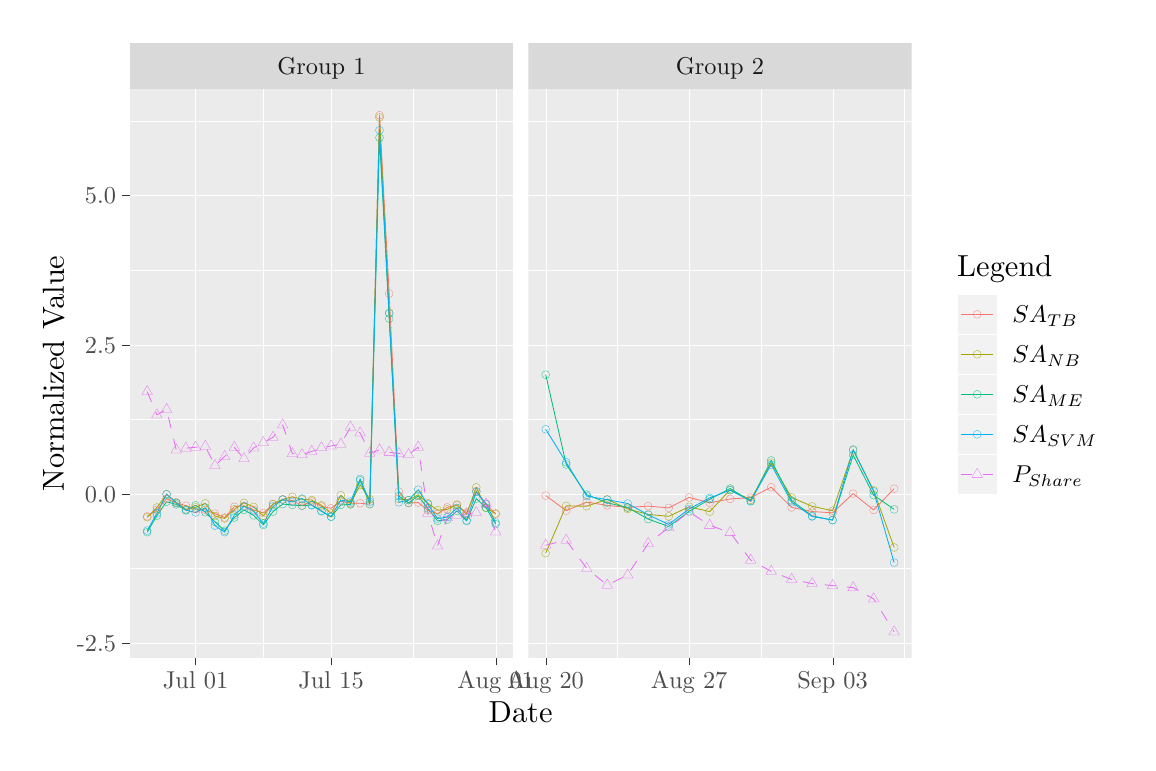
\begin{tikzpicture}[x=1pt,y=1pt]
\definecolor{fillColor}{RGB}{255,255,255}
\path[use as bounding box,fill=fillColor,fill opacity=0.00] (0,0) rectangle (397.48,258.37);
\begin{scope}
\path[clip] (  0.00,  0.00) rectangle (397.48,258.37);
\definecolor{drawColor}{RGB}{255,255,255}
\definecolor{fillColor}{RGB}{255,255,255}

\path[draw=drawColor,line width= 0.1pt,line join=round,line cap=round,fill=fillColor] (  0.00, -0.00) rectangle (397.48,258.37);
\end{scope}
\begin{scope}
\path[clip] ( 36.90, 30.73) rectangle (175.39,236.06);
\definecolor{fillColor}{gray}{0.92}

\path[fill=fillColor] ( 36.90, 30.73) rectangle (175.39,236.06);
\definecolor{drawColor}{RGB}{255,255,255}

\path[draw=drawColor,line width= 0.1pt,line join=round] ( 36.90, 62.94) --
	(175.39, 62.94);

\path[draw=drawColor,line width= 0.1pt,line join=round] ( 36.90,116.85) --
	(175.39,116.85);

\path[draw=drawColor,line width= 0.1pt,line join=round] ( 36.90,170.76) --
	(175.39,170.76);

\path[draw=drawColor,line width= 0.1pt,line join=round] ( 36.90,224.68) --
	(175.39,224.68);

\path[draw=drawColor,line width= 0.1pt,line join=round] ( 85.16, 30.73) --
	( 85.16,236.06);

\path[draw=drawColor,line width= 0.1pt,line join=round] (139.37, 30.73) --
	(139.37,236.06);

\path[draw=drawColor,line width= 0.1pt,line join=round] ( 36.90, 35.99) --
	(175.39, 35.99);

\path[draw=drawColor,line width= 0.1pt,line join=round] ( 36.90, 89.90) --
	(175.39, 89.90);

\path[draw=drawColor,line width= 0.1pt,line join=round] ( 36.90,143.81) --
	(175.39,143.81);

\path[draw=drawColor,line width= 0.1pt,line join=round] ( 36.90,197.72) --
	(175.39,197.72);

\path[draw=drawColor,line width= 0.1pt,line join=round] ( 60.68, 30.73) --
	( 60.68,236.06);

\path[draw=drawColor,line width= 0.1pt,line join=round] (109.64, 30.73) --
	(109.64,236.06);

\path[draw=drawColor,line width= 0.1pt,line join=round] (169.10, 30.73) --
	(169.10,236.06);
\definecolor{drawColor}{RGB}{248,118,109}

\path[draw=drawColor,line width= 0.3pt,line join=round] ( 43.20, 81.79) --
	( 46.69, 84.10) --
	( 50.19, 88.13) --
	( 53.69, 86.63) --
	( 57.18, 85.65) --
	( 60.68, 84.36) --
	( 64.18, 84.10) --
	( 67.68, 82.76) --
	( 71.17, 81.37) --
	( 74.67, 85.25) --
	( 78.17, 85.59) --
	( 81.67, 84.11) --
	( 85.16, 82.99) --
	( 88.66, 86.17) --
	( 92.16, 87.87) --
	( 95.65, 87.51) --
	( 99.15, 85.74) --
	(102.65, 87.16) --
	(106.15, 85.38) --
	(109.64, 84.69) --
	(113.14, 87.29) --
	(116.64, 86.55) --
	(120.14, 86.52) --
	(123.63, 86.20) --
	(127.13,226.73) --
	(130.63,162.31) --
	(134.13, 90.71) --
	(137.62, 86.64) --
	(141.12, 86.77) --
	(144.62, 83.97) --
	(148.11, 82.74) --
	(151.61, 85.02) --
	(155.11, 85.83) --
	(158.61, 83.10) --
	(162.10, 90.95) --
	(165.60, 86.36) --
	(169.10, 82.56);
\definecolor{drawColor}{RGB}{163,165,0}

\path[draw=drawColor,line width= 0.3pt,line join=round] ( 43.20, 81.47) --
	( 46.69, 84.97) --
	( 50.19, 89.75) --
	( 53.69, 86.84) --
	( 57.18, 84.35) --
	( 60.68, 85.05) --
	( 64.18, 86.49) --
	( 67.68, 81.90) --
	( 71.17, 81.02) --
	( 74.67, 84.33) --
	( 78.17, 86.66) --
	( 81.67, 85.19) --
	( 85.16, 81.98) --
	( 88.66, 86.27) --
	( 92.16, 87.94) --
	( 95.65, 88.83) --
	( 99.15, 87.94) --
	(102.65, 87.67) --
	(106.15, 85.77) --
	(109.64, 82.85) --
	(113.14, 89.44) --
	(116.64, 86.37) --
	(120.14, 93.12) --
	(123.63, 87.97) --
	(127.13,225.91) --
	(130.63,155.35) --
	(134.13, 88.12) --
	(137.62, 87.62) --
	(141.12, 89.60) --
	(144.62, 86.51) --
	(148.11, 84.02) --
	(151.61, 84.30) --
	(155.11, 86.01) --
	(158.61, 82.48) --
	(162.10, 92.29) --
	(165.60, 84.85) --
	(169.10, 82.84);
\definecolor{drawColor}{RGB}{0,191,125}

\path[draw=drawColor,line width= 0.3pt,line join=round] ( 43.20, 76.06) --
	( 46.69, 82.03) --
	( 50.19, 87.08) --
	( 53.69, 86.09) --
	( 57.18, 83.95) --
	( 60.68, 85.79) --
	( 64.18, 83.28) --
	( 67.68, 79.79) --
	( 71.17, 76.59) --
	( 74.67, 81.35) --
	( 78.17, 84.11) --
	( 81.67, 82.13) --
	( 85.16, 78.68) --
	( 88.66, 83.52) --
	( 92.16, 86.21) --
	( 95.65, 85.90) --
	( 99.15, 85.60) --
	(102.65, 85.93) --
	(106.15, 83.75) --
	(109.64, 81.60) --
	(113.14, 85.91) --
	(116.64, 86.09) --
	(120.14, 94.77) --
	(123.63, 86.21) --
	(127.13,218.60) --
	(130.63,153.23) --
	(134.13, 89.12) --
	(137.62, 86.64) --
	(141.12, 89.16) --
	(144.62, 84.63) --
	(148.11, 80.17) --
	(151.61, 80.61) --
	(155.11, 83.73) --
	(158.61, 80.11) --
	(162.10, 88.19) --
	(165.60, 84.95) --
	(169.10, 78.96);
\definecolor{drawColor}{RGB}{0,176,246}

\path[draw=drawColor,line width= 0.3pt,line join=round] ( 43.20, 76.64) --
	( 46.69, 82.90) --
	( 50.19, 89.82) --
	( 53.69, 86.63) --
	( 57.18, 84.03) --
	( 60.68, 83.18) --
	( 64.18, 84.89) --
	( 67.68, 78.43) --
	( 71.17, 76.07) --
	( 74.67, 82.23) --
	( 78.17, 85.39) --
	( 81.67, 83.61) --
	( 85.16, 79.19) --
	( 88.66, 85.37) --
	( 92.16, 87.83) --
	( 95.65, 86.98) --
	( 99.15, 88.23) --
	(102.65, 85.79) --
	(106.15, 83.61) --
	(109.64, 81.72) --
	(113.14, 87.67) --
	(116.64, 87.12) --
	(120.14, 95.33) --
	(123.63, 87.05) --
	(127.13,221.32) --
	(130.63,155.11) --
	(134.13, 86.87) --
	(137.62, 87.64) --
	(141.12, 91.42) --
	(144.62, 86.15) --
	(148.11, 80.96) --
	(151.61, 81.54) --
	(155.11, 84.88) --
	(158.61, 80.34) --
	(162.10, 90.67) --
	(165.60, 86.26) --
	(169.10, 79.55);
\definecolor{drawColor}{RGB}{231,107,243}

\path[draw=drawColor,line width= 0.3pt,dash pattern=on 4pt off 4pt ,line join=round] ( 43.20,126.85) --
	( 46.69,118.47) --
	( 50.19,120.44) --
	( 53.69,105.78) --
	( 57.18,106.43) --
	( 60.68,106.76) --
	( 64.18,107.09) --
	( 67.68,100.15) --
	( 71.17,103.42) --
	( 74.67,106.69) --
	( 78.17,102.63) --
	( 81.67,106.50) --
	( 85.16,108.43) --
	( 88.66,110.36) --
	( 92.16,114.81) --
	( 95.65,104.47) --
	( 99.15,104.07) --
	(102.65,105.25) --
	(106.15,106.56) --
	(109.64,107.22) --
	(113.14,107.87) --
	(116.64,114.02) --
	(120.14,111.93) --
	(123.63,104.60) --
	(127.13,105.78) --
	(130.63,104.93) --
	(134.13,104.50) --
	(137.62,104.07) --
	(141.12,106.82) --
	(144.62, 82.87) --
	(148.11, 71.09) --
	(151.61, 81.30) --
	(155.11, 82.21) --
	(158.61, 82.67) --
	(162.10, 83.13) --
	(165.60, 86.27) --
	(169.10, 76.19);
\definecolor{drawColor}{RGB}{248,118,109}

\path[draw=drawColor,line width= 0.1pt,line join=round,line cap=round] ( 43.20, 81.79) circle (  1.43);

\path[draw=drawColor,line width= 0.1pt,line join=round,line cap=round] ( 46.69, 84.10) circle (  1.43);

\path[draw=drawColor,line width= 0.1pt,line join=round,line cap=round] ( 50.19, 88.13) circle (  1.43);

\path[draw=drawColor,line width= 0.1pt,line join=round,line cap=round] ( 53.69, 86.63) circle (  1.43);

\path[draw=drawColor,line width= 0.1pt,line join=round,line cap=round] ( 57.18, 85.65) circle (  1.43);

\path[draw=drawColor,line width= 0.1pt,line join=round,line cap=round] ( 60.68, 84.36) circle (  1.43);

\path[draw=drawColor,line width= 0.1pt,line join=round,line cap=round] ( 64.18, 84.10) circle (  1.43);

\path[draw=drawColor,line width= 0.1pt,line join=round,line cap=round] ( 67.68, 82.76) circle (  1.43);

\path[draw=drawColor,line width= 0.1pt,line join=round,line cap=round] ( 71.17, 81.37) circle (  1.43);

\path[draw=drawColor,line width= 0.1pt,line join=round,line cap=round] ( 74.67, 85.25) circle (  1.43);

\path[draw=drawColor,line width= 0.1pt,line join=round,line cap=round] ( 78.17, 85.59) circle (  1.43);

\path[draw=drawColor,line width= 0.1pt,line join=round,line cap=round] ( 81.67, 84.11) circle (  1.43);

\path[draw=drawColor,line width= 0.1pt,line join=round,line cap=round] ( 85.16, 82.99) circle (  1.43);

\path[draw=drawColor,line width= 0.1pt,line join=round,line cap=round] ( 88.66, 86.17) circle (  1.43);

\path[draw=drawColor,line width= 0.1pt,line join=round,line cap=round] ( 92.16, 87.87) circle (  1.43);

\path[draw=drawColor,line width= 0.1pt,line join=round,line cap=round] ( 95.65, 87.51) circle (  1.43);

\path[draw=drawColor,line width= 0.1pt,line join=round,line cap=round] ( 99.15, 85.74) circle (  1.43);

\path[draw=drawColor,line width= 0.1pt,line join=round,line cap=round] (102.65, 87.16) circle (  1.43);

\path[draw=drawColor,line width= 0.1pt,line join=round,line cap=round] (106.15, 85.38) circle (  1.43);

\path[draw=drawColor,line width= 0.1pt,line join=round,line cap=round] (109.64, 84.69) circle (  1.43);

\path[draw=drawColor,line width= 0.1pt,line join=round,line cap=round] (113.14, 87.29) circle (  1.43);

\path[draw=drawColor,line width= 0.1pt,line join=round,line cap=round] (116.64, 86.55) circle (  1.43);

\path[draw=drawColor,line width= 0.1pt,line join=round,line cap=round] (120.14, 86.52) circle (  1.43);

\path[draw=drawColor,line width= 0.1pt,line join=round,line cap=round] (123.63, 86.20) circle (  1.43);

\path[draw=drawColor,line width= 0.1pt,line join=round,line cap=round] (127.13,226.73) circle (  1.43);

\path[draw=drawColor,line width= 0.1pt,line join=round,line cap=round] (130.63,162.31) circle (  1.43);

\path[draw=drawColor,line width= 0.1pt,line join=round,line cap=round] (134.13, 90.71) circle (  1.43);

\path[draw=drawColor,line width= 0.1pt,line join=round,line cap=round] (137.62, 86.64) circle (  1.43);

\path[draw=drawColor,line width= 0.1pt,line join=round,line cap=round] (141.12, 86.77) circle (  1.43);

\path[draw=drawColor,line width= 0.1pt,line join=round,line cap=round] (144.62, 83.97) circle (  1.43);

\path[draw=drawColor,line width= 0.1pt,line join=round,line cap=round] (148.11, 82.74) circle (  1.43);

\path[draw=drawColor,line width= 0.1pt,line join=round,line cap=round] (151.61, 85.02) circle (  1.43);

\path[draw=drawColor,line width= 0.1pt,line join=round,line cap=round] (155.11, 85.83) circle (  1.43);

\path[draw=drawColor,line width= 0.1pt,line join=round,line cap=round] (158.61, 83.10) circle (  1.43);

\path[draw=drawColor,line width= 0.1pt,line join=round,line cap=round] (162.10, 90.95) circle (  1.43);

\path[draw=drawColor,line width= 0.1pt,line join=round,line cap=round] (165.60, 86.36) circle (  1.43);

\path[draw=drawColor,line width= 0.1pt,line join=round,line cap=round] (169.10, 82.56) circle (  1.43);
\definecolor{drawColor}{RGB}{163,165,0}

\path[draw=drawColor,line width= 0.1pt,line join=round,line cap=round] ( 43.20, 81.47) circle (  1.43);

\path[draw=drawColor,line width= 0.1pt,line join=round,line cap=round] ( 46.69, 84.97) circle (  1.43);

\path[draw=drawColor,line width= 0.1pt,line join=round,line cap=round] ( 50.19, 89.75) circle (  1.43);

\path[draw=drawColor,line width= 0.1pt,line join=round,line cap=round] ( 53.69, 86.84) circle (  1.43);

\path[draw=drawColor,line width= 0.1pt,line join=round,line cap=round] ( 57.18, 84.35) circle (  1.43);

\path[draw=drawColor,line width= 0.1pt,line join=round,line cap=round] ( 60.68, 85.05) circle (  1.43);

\path[draw=drawColor,line width= 0.1pt,line join=round,line cap=round] ( 64.18, 86.49) circle (  1.43);

\path[draw=drawColor,line width= 0.1pt,line join=round,line cap=round] ( 67.68, 81.90) circle (  1.43);

\path[draw=drawColor,line width= 0.1pt,line join=round,line cap=round] ( 71.17, 81.02) circle (  1.43);

\path[draw=drawColor,line width= 0.1pt,line join=round,line cap=round] ( 74.67, 84.33) circle (  1.43);

\path[draw=drawColor,line width= 0.1pt,line join=round,line cap=round] ( 78.17, 86.66) circle (  1.43);

\path[draw=drawColor,line width= 0.1pt,line join=round,line cap=round] ( 81.67, 85.19) circle (  1.43);

\path[draw=drawColor,line width= 0.1pt,line join=round,line cap=round] ( 85.16, 81.98) circle (  1.43);

\path[draw=drawColor,line width= 0.1pt,line join=round,line cap=round] ( 88.66, 86.27) circle (  1.43);

\path[draw=drawColor,line width= 0.1pt,line join=round,line cap=round] ( 92.16, 87.94) circle (  1.43);

\path[draw=drawColor,line width= 0.1pt,line join=round,line cap=round] ( 95.65, 88.83) circle (  1.43);

\path[draw=drawColor,line width= 0.1pt,line join=round,line cap=round] ( 99.15, 87.94) circle (  1.43);

\path[draw=drawColor,line width= 0.1pt,line join=round,line cap=round] (102.65, 87.67) circle (  1.43);

\path[draw=drawColor,line width= 0.1pt,line join=round,line cap=round] (106.15, 85.77) circle (  1.43);

\path[draw=drawColor,line width= 0.1pt,line join=round,line cap=round] (109.64, 82.85) circle (  1.43);

\path[draw=drawColor,line width= 0.1pt,line join=round,line cap=round] (113.14, 89.44) circle (  1.43);

\path[draw=drawColor,line width= 0.1pt,line join=round,line cap=round] (116.64, 86.37) circle (  1.43);

\path[draw=drawColor,line width= 0.1pt,line join=round,line cap=round] (120.14, 93.12) circle (  1.43);

\path[draw=drawColor,line width= 0.1pt,line join=round,line cap=round] (123.63, 87.97) circle (  1.43);

\path[draw=drawColor,line width= 0.1pt,line join=round,line cap=round] (127.13,225.91) circle (  1.43);

\path[draw=drawColor,line width= 0.1pt,line join=round,line cap=round] (130.63,155.35) circle (  1.43);

\path[draw=drawColor,line width= 0.1pt,line join=round,line cap=round] (134.13, 88.12) circle (  1.43);

\path[draw=drawColor,line width= 0.1pt,line join=round,line cap=round] (137.62, 87.62) circle (  1.43);

\path[draw=drawColor,line width= 0.1pt,line join=round,line cap=round] (141.12, 89.60) circle (  1.43);

\path[draw=drawColor,line width= 0.1pt,line join=round,line cap=round] (144.62, 86.51) circle (  1.43);

\path[draw=drawColor,line width= 0.1pt,line join=round,line cap=round] (148.11, 84.02) circle (  1.43);

\path[draw=drawColor,line width= 0.1pt,line join=round,line cap=round] (151.61, 84.30) circle (  1.43);

\path[draw=drawColor,line width= 0.1pt,line join=round,line cap=round] (155.11, 86.01) circle (  1.43);

\path[draw=drawColor,line width= 0.1pt,line join=round,line cap=round] (158.61, 82.48) circle (  1.43);

\path[draw=drawColor,line width= 0.1pt,line join=round,line cap=round] (162.10, 92.29) circle (  1.43);

\path[draw=drawColor,line width= 0.1pt,line join=round,line cap=round] (165.60, 84.85) circle (  1.43);

\path[draw=drawColor,line width= 0.1pt,line join=round,line cap=round] (169.10, 82.84) circle (  1.43);
\definecolor{drawColor}{RGB}{0,191,125}

\path[draw=drawColor,line width= 0.1pt,line join=round,line cap=round] ( 43.20, 76.06) circle (  1.43);

\path[draw=drawColor,line width= 0.1pt,line join=round,line cap=round] ( 46.69, 82.03) circle (  1.43);

\path[draw=drawColor,line width= 0.1pt,line join=round,line cap=round] ( 50.19, 87.08) circle (  1.43);

\path[draw=drawColor,line width= 0.1pt,line join=round,line cap=round] ( 53.69, 86.09) circle (  1.43);

\path[draw=drawColor,line width= 0.1pt,line join=round,line cap=round] ( 57.18, 83.95) circle (  1.43);

\path[draw=drawColor,line width= 0.1pt,line join=round,line cap=round] ( 60.68, 85.79) circle (  1.43);

\path[draw=drawColor,line width= 0.1pt,line join=round,line cap=round] ( 64.18, 83.28) circle (  1.43);

\path[draw=drawColor,line width= 0.1pt,line join=round,line cap=round] ( 67.68, 79.79) circle (  1.43);

\path[draw=drawColor,line width= 0.1pt,line join=round,line cap=round] ( 71.17, 76.59) circle (  1.43);

\path[draw=drawColor,line width= 0.1pt,line join=round,line cap=round] ( 74.67, 81.35) circle (  1.43);

\path[draw=drawColor,line width= 0.1pt,line join=round,line cap=round] ( 78.17, 84.11) circle (  1.43);

\path[draw=drawColor,line width= 0.1pt,line join=round,line cap=round] ( 81.67, 82.13) circle (  1.43);

\path[draw=drawColor,line width= 0.1pt,line join=round,line cap=round] ( 85.16, 78.68) circle (  1.43);

\path[draw=drawColor,line width= 0.1pt,line join=round,line cap=round] ( 88.66, 83.52) circle (  1.43);

\path[draw=drawColor,line width= 0.1pt,line join=round,line cap=round] ( 92.16, 86.21) circle (  1.43);

\path[draw=drawColor,line width= 0.1pt,line join=round,line cap=round] ( 95.65, 85.90) circle (  1.43);

\path[draw=drawColor,line width= 0.1pt,line join=round,line cap=round] ( 99.15, 85.60) circle (  1.43);

\path[draw=drawColor,line width= 0.1pt,line join=round,line cap=round] (102.65, 85.93) circle (  1.43);

\path[draw=drawColor,line width= 0.1pt,line join=round,line cap=round] (106.15, 83.75) circle (  1.43);

\path[draw=drawColor,line width= 0.1pt,line join=round,line cap=round] (109.64, 81.60) circle (  1.43);

\path[draw=drawColor,line width= 0.1pt,line join=round,line cap=round] (113.14, 85.91) circle (  1.43);

\path[draw=drawColor,line width= 0.1pt,line join=round,line cap=round] (116.64, 86.09) circle (  1.43);

\path[draw=drawColor,line width= 0.1pt,line join=round,line cap=round] (120.14, 94.77) circle (  1.43);

\path[draw=drawColor,line width= 0.1pt,line join=round,line cap=round] (123.63, 86.21) circle (  1.43);

\path[draw=drawColor,line width= 0.1pt,line join=round,line cap=round] (127.13,218.60) circle (  1.43);

\path[draw=drawColor,line width= 0.1pt,line join=round,line cap=round] (130.63,153.23) circle (  1.43);

\path[draw=drawColor,line width= 0.1pt,line join=round,line cap=round] (134.13, 89.12) circle (  1.43);

\path[draw=drawColor,line width= 0.1pt,line join=round,line cap=round] (137.62, 86.64) circle (  1.43);

\path[draw=drawColor,line width= 0.1pt,line join=round,line cap=round] (141.12, 89.16) circle (  1.43);

\path[draw=drawColor,line width= 0.1pt,line join=round,line cap=round] (144.62, 84.63) circle (  1.43);

\path[draw=drawColor,line width= 0.1pt,line join=round,line cap=round] (148.11, 80.17) circle (  1.43);

\path[draw=drawColor,line width= 0.1pt,line join=round,line cap=round] (151.61, 80.61) circle (  1.43);

\path[draw=drawColor,line width= 0.1pt,line join=round,line cap=round] (155.11, 83.73) circle (  1.43);

\path[draw=drawColor,line width= 0.1pt,line join=round,line cap=round] (158.61, 80.11) circle (  1.43);

\path[draw=drawColor,line width= 0.1pt,line join=round,line cap=round] (162.10, 88.19) circle (  1.43);

\path[draw=drawColor,line width= 0.1pt,line join=round,line cap=round] (165.60, 84.95) circle (  1.43);

\path[draw=drawColor,line width= 0.1pt,line join=round,line cap=round] (169.10, 78.96) circle (  1.43);
\definecolor{drawColor}{RGB}{0,176,246}

\path[draw=drawColor,line width= 0.1pt,line join=round,line cap=round] ( 43.20, 76.64) circle (  1.43);

\path[draw=drawColor,line width= 0.1pt,line join=round,line cap=round] ( 46.69, 82.90) circle (  1.43);

\path[draw=drawColor,line width= 0.1pt,line join=round,line cap=round] ( 50.19, 89.82) circle (  1.43);

\path[draw=drawColor,line width= 0.1pt,line join=round,line cap=round] ( 53.69, 86.63) circle (  1.43);

\path[draw=drawColor,line width= 0.1pt,line join=round,line cap=round] ( 57.18, 84.03) circle (  1.43);

\path[draw=drawColor,line width= 0.1pt,line join=round,line cap=round] ( 60.68, 83.18) circle (  1.43);

\path[draw=drawColor,line width= 0.1pt,line join=round,line cap=round] ( 64.18, 84.89) circle (  1.43);

\path[draw=drawColor,line width= 0.1pt,line join=round,line cap=round] ( 67.68, 78.43) circle (  1.43);

\path[draw=drawColor,line width= 0.1pt,line join=round,line cap=round] ( 71.17, 76.07) circle (  1.43);

\path[draw=drawColor,line width= 0.1pt,line join=round,line cap=round] ( 74.67, 82.23) circle (  1.43);

\path[draw=drawColor,line width= 0.1pt,line join=round,line cap=round] ( 78.17, 85.39) circle (  1.43);

\path[draw=drawColor,line width= 0.1pt,line join=round,line cap=round] ( 81.67, 83.61) circle (  1.43);

\path[draw=drawColor,line width= 0.1pt,line join=round,line cap=round] ( 85.16, 79.19) circle (  1.43);

\path[draw=drawColor,line width= 0.1pt,line join=round,line cap=round] ( 88.66, 85.37) circle (  1.43);

\path[draw=drawColor,line width= 0.1pt,line join=round,line cap=round] ( 92.16, 87.83) circle (  1.43);

\path[draw=drawColor,line width= 0.1pt,line join=round,line cap=round] ( 95.65, 86.98) circle (  1.43);

\path[draw=drawColor,line width= 0.1pt,line join=round,line cap=round] ( 99.15, 88.23) circle (  1.43);

\path[draw=drawColor,line width= 0.1pt,line join=round,line cap=round] (102.65, 85.79) circle (  1.43);

\path[draw=drawColor,line width= 0.1pt,line join=round,line cap=round] (106.15, 83.61) circle (  1.43);

\path[draw=drawColor,line width= 0.1pt,line join=round,line cap=round] (109.64, 81.72) circle (  1.43);

\path[draw=drawColor,line width= 0.1pt,line join=round,line cap=round] (113.14, 87.67) circle (  1.43);

\path[draw=drawColor,line width= 0.1pt,line join=round,line cap=round] (116.64, 87.12) circle (  1.43);

\path[draw=drawColor,line width= 0.1pt,line join=round,line cap=round] (120.14, 95.33) circle (  1.43);

\path[draw=drawColor,line width= 0.1pt,line join=round,line cap=round] (123.63, 87.05) circle (  1.43);

\path[draw=drawColor,line width= 0.1pt,line join=round,line cap=round] (127.13,221.32) circle (  1.43);

\path[draw=drawColor,line width= 0.1pt,line join=round,line cap=round] (130.63,155.11) circle (  1.43);

\path[draw=drawColor,line width= 0.1pt,line join=round,line cap=round] (134.13, 86.87) circle (  1.43);

\path[draw=drawColor,line width= 0.1pt,line join=round,line cap=round] (137.62, 87.64) circle (  1.43);

\path[draw=drawColor,line width= 0.1pt,line join=round,line cap=round] (141.12, 91.42) circle (  1.43);

\path[draw=drawColor,line width= 0.1pt,line join=round,line cap=round] (144.62, 86.15) circle (  1.43);

\path[draw=drawColor,line width= 0.1pt,line join=round,line cap=round] (148.11, 80.96) circle (  1.43);

\path[draw=drawColor,line width= 0.1pt,line join=round,line cap=round] (151.61, 81.54) circle (  1.43);

\path[draw=drawColor,line width= 0.1pt,line join=round,line cap=round] (155.11, 84.88) circle (  1.43);

\path[draw=drawColor,line width= 0.1pt,line join=round,line cap=round] (158.61, 80.34) circle (  1.43);

\path[draw=drawColor,line width= 0.1pt,line join=round,line cap=round] (162.10, 90.67) circle (  1.43);

\path[draw=drawColor,line width= 0.1pt,line join=round,line cap=round] (165.60, 86.26) circle (  1.43);

\path[draw=drawColor,line width= 0.1pt,line join=round,line cap=round] (169.10, 79.55) circle (  1.43);
\definecolor{drawColor}{RGB}{231,107,243}

\path[draw=drawColor,line width= 0.1pt,line join=round,line cap=round] ( 43.20,129.07) --
	( 45.12,125.74) --
	( 41.27,125.74) --
	( 43.20,129.07);

\path[draw=drawColor,line width= 0.1pt,line join=round,line cap=round] ( 46.69,120.69) --
	( 48.61,117.36) --
	( 44.77,117.36) --
	( 46.69,120.69);

\path[draw=drawColor,line width= 0.1pt,line join=round,line cap=round] ( 50.19,122.66) --
	( 52.11,119.33) --
	( 48.27,119.33) --
	( 50.19,122.66);

\path[draw=drawColor,line width= 0.1pt,line join=round,line cap=round] ( 53.69,107.99) --
	( 55.61,104.67) --
	( 51.77,104.67) --
	( 53.69,107.99);

\path[draw=drawColor,line width= 0.1pt,line join=round,line cap=round] ( 57.18,108.65) --
	( 59.11,105.32) --
	( 55.26,105.32) --
	( 57.18,108.65);

\path[draw=drawColor,line width= 0.1pt,line join=round,line cap=round] ( 60.68,108.98) --
	( 62.60,105.65) --
	( 58.76,105.65) --
	( 60.68,108.98);

\path[draw=drawColor,line width= 0.1pt,line join=round,line cap=round] ( 64.18,109.30) --
	( 66.10,105.98) --
	( 62.26,105.98) --
	( 64.18,109.30);

\path[draw=drawColor,line width= 0.1pt,line join=round,line cap=round] ( 67.68,102.37) --
	( 69.60, 99.04) --
	( 65.75, 99.04) --
	( 67.68,102.37);

\path[draw=drawColor,line width= 0.1pt,line join=round,line cap=round] ( 71.17,105.64) --
	( 73.09,102.31) --
	( 69.25,102.31) --
	( 71.17,105.64);

\path[draw=drawColor,line width= 0.1pt,line join=round,line cap=round] ( 74.67,108.91) --
	( 76.59,105.58) --
	( 72.75,105.58) --
	( 74.67,108.91);

\path[draw=drawColor,line width= 0.1pt,line join=round,line cap=round] ( 78.17,104.85) --
	( 80.09,101.53) --
	( 76.25,101.53) --
	( 78.17,104.85);

\path[draw=drawColor,line width= 0.1pt,line join=round,line cap=round] ( 81.67,108.71) --
	( 83.59,105.39) --
	( 79.74,105.39) --
	( 81.67,108.71);

\path[draw=drawColor,line width= 0.1pt,line join=round,line cap=round] ( 85.16,110.65) --
	( 87.08,107.32) --
	( 83.24,107.32) --
	( 85.16,110.65);

\path[draw=drawColor,line width= 0.1pt,line join=round,line cap=round] ( 88.66,112.58) --
	( 90.58,109.25) --
	( 86.74,109.25) --
	( 88.66,112.58);

\path[draw=drawColor,line width= 0.1pt,line join=round,line cap=round] ( 92.16,117.03) --
	( 94.08,113.70) --
	( 90.24,113.70) --
	( 92.16,117.03);

\path[draw=drawColor,line width= 0.1pt,line join=round,line cap=round] ( 95.65,106.69) --
	( 97.58,103.36) --
	( 93.73,103.36) --
	( 95.65,106.69);

\path[draw=drawColor,line width= 0.1pt,line join=round,line cap=round] ( 99.15,106.29) --
	(101.07,102.96) --
	( 97.23,102.96) --
	( 99.15,106.29);

\path[draw=drawColor,line width= 0.1pt,line join=round,line cap=round] (102.65,107.47) --
	(104.57,104.14) --
	(100.73,104.14) --
	(102.65,107.47);

\path[draw=drawColor,line width= 0.1pt,line join=round,line cap=round] (106.15,108.78) --
	(108.07,105.45) --
	(104.23,105.45) --
	(106.15,108.78);

\path[draw=drawColor,line width= 0.1pt,line join=round,line cap=round] (109.64,109.43) --
	(111.57,106.11) --
	(107.72,106.11) --
	(109.64,109.43);

\path[draw=drawColor,line width= 0.1pt,line join=round,line cap=round] (113.14,110.09) --
	(115.06,106.76) --
	(111.22,106.76) --
	(113.14,110.09);

\path[draw=drawColor,line width= 0.1pt,line join=round,line cap=round] (116.64,116.24) --
	(118.56,112.91) --
	(114.72,112.91) --
	(116.64,116.24);

\path[draw=drawColor,line width= 0.1pt,line join=round,line cap=round] (120.14,114.15) --
	(122.06,110.82) --
	(118.21,110.82) --
	(120.14,114.15);

\path[draw=drawColor,line width= 0.1pt,line join=round,line cap=round] (123.63,106.82) --
	(125.55,103.49) --
	(121.71,103.49) --
	(123.63,106.82);

\path[draw=drawColor,line width= 0.1pt,line join=round,line cap=round] (127.13,107.99) --
	(129.05,104.67) --
	(125.21,104.67) --
	(127.13,107.99);

\path[draw=drawColor,line width= 0.1pt,line join=round,line cap=round] (130.63,107.14) --
	(132.55,103.82) --
	(128.71,103.82) --
	(130.63,107.14);

\path[draw=drawColor,line width= 0.1pt,line join=round,line cap=round] (134.13,106.72) --
	(136.05,103.39) --
	(132.20,103.39) --
	(134.13,106.72);

\path[draw=drawColor,line width= 0.1pt,line join=round,line cap=round] (137.62,106.29) --
	(139.54,102.96) --
	(135.70,102.96) --
	(137.62,106.29);

\path[draw=drawColor,line width= 0.1pt,line join=round,line cap=round] (141.12,109.04) --
	(143.04,105.71) --
	(139.20,105.71) --
	(141.12,109.04);

\path[draw=drawColor,line width= 0.1pt,line join=round,line cap=round] (144.62, 85.09) --
	(146.54, 81.76) --
	(142.70, 81.76) --
	(144.62, 85.09);

\path[draw=drawColor,line width= 0.1pt,line join=round,line cap=round] (148.11, 73.30) --
	(150.04, 69.98) --
	(146.19, 69.98) --
	(148.11, 73.30);

\path[draw=drawColor,line width= 0.1pt,line join=round,line cap=round] (151.61, 83.52) --
	(153.53, 80.19) --
	(149.69, 80.19) --
	(151.61, 83.52);

\path[draw=drawColor,line width= 0.1pt,line join=round,line cap=round] (155.11, 84.43) --
	(157.03, 81.10) --
	(153.19, 81.10) --
	(155.11, 84.43);

\path[draw=drawColor,line width= 0.1pt,line join=round,line cap=round] (158.61, 84.89) --
	(160.53, 81.56) --
	(156.69, 81.56) --
	(158.61, 84.89);

\path[draw=drawColor,line width= 0.1pt,line join=round,line cap=round] (162.10, 85.35) --
	(164.03, 82.02) --
	(160.18, 82.02) --
	(162.10, 85.35);

\path[draw=drawColor,line width= 0.1pt,line join=round,line cap=round] (165.60, 88.49) --
	(167.52, 85.16) --
	(163.68, 85.16) --
	(165.60, 88.49);

\path[draw=drawColor,line width= 0.1pt,line join=round,line cap=round] (169.10, 78.41) --
	(171.02, 75.08) --
	(167.18, 75.08) --
	(169.10, 78.41);
\end{scope}
\begin{scope}
\path[clip] (180.89, 30.73) rectangle (319.39,236.06);
\definecolor{fillColor}{gray}{0.92}

\path[fill=fillColor] (180.89, 30.73) rectangle (319.39,236.06);
\definecolor{drawColor}{RGB}{255,255,255}

\path[draw=drawColor,line width= 0.1pt,line join=round] (180.89, 62.94) --
	(319.39, 62.94);

\path[draw=drawColor,line width= 0.1pt,line join=round] (180.89,116.85) --
	(319.39,116.85);

\path[draw=drawColor,line width= 0.1pt,line join=round] (180.89,170.76) --
	(319.39,170.76);

\path[draw=drawColor,line width= 0.1pt,line join=round] (180.89,224.68) --
	(319.39,224.68);

\path[draw=drawColor,line width= 0.1pt,line join=round] (213.11, 30.73) --
	(213.11,236.06);

\path[draw=drawColor,line width= 0.1pt,line join=round] (264.95, 30.73) --
	(264.95,236.06);

\path[draw=drawColor,line width= 0.1pt,line join=round] (316.80, 30.73) --
	(316.80,236.06);

\path[draw=drawColor,line width= 0.1pt,line join=round] (180.89, 35.99) --
	(319.39, 35.99);

\path[draw=drawColor,line width= 0.1pt,line join=round] (180.89, 89.90) --
	(319.39, 89.90);

\path[draw=drawColor,line width= 0.1pt,line join=round] (180.89,143.81) --
	(319.39,143.81);

\path[draw=drawColor,line width= 0.1pt,line join=round] (180.89,197.72) --
	(319.39,197.72);

\path[draw=drawColor,line width= 0.1pt,line join=round] (187.19, 30.73) --
	(187.19,236.06);

\path[draw=drawColor,line width= 0.1pt,line join=round] (239.03, 30.73) --
	(239.03,236.06);

\path[draw=drawColor,line width= 0.1pt,line join=round] (290.87, 30.73) --
	(290.87,236.06);
\definecolor{drawColor}{RGB}{248,118,109}

\path[draw=drawColor,line width= 0.3pt,line join=round] (187.19, 89.30) --
	(194.59, 83.84) --
	(202.00, 86.94) --
	(209.41, 85.76) --
	(216.81, 84.99) --
	(224.22, 85.48) --
	(231.63, 84.85) --
	(239.03, 88.61) --
	(246.44, 86.69) --
	(253.84, 88.07) --
	(261.25, 88.55) --
	(268.66, 92.33) --
	(276.06, 85.00) --
	(283.47, 83.52) --
	(290.87, 83.07) --
	(298.28, 90.01) --
	(305.69, 84.10) --
	(313.09, 91.78);
\definecolor{drawColor}{RGB}{163,165,0}

\path[draw=drawColor,line width= 0.3pt,line join=round] (187.19, 68.48) --
	(194.59, 85.59) --
	(202.00, 85.43) --
	(209.41, 87.94) --
	(216.81, 84.46) --
	(224.22, 82.48) --
	(231.63, 81.79) --
	(239.03, 85.25) --
	(246.44, 83.49) --
	(253.84, 91.38) --
	(261.25, 87.75) --
	(268.66,101.13) --
	(276.06, 88.59) --
	(283.47, 85.42) --
	(290.87, 83.83) --
	(298.28,105.65) --
	(305.69, 91.21) --
	(313.09, 70.55);
\definecolor{drawColor}{RGB}{0,191,125}

\path[draw=drawColor,line width= 0.3pt,line join=round] (187.19,132.98) --
	(194.59,100.55) --
	(202.00, 89.63) --
	(209.41, 86.69) --
	(216.81, 84.98) --
	(224.22, 80.79) --
	(231.63, 78.15) --
	(239.03, 83.60) --
	(246.44, 87.97) --
	(253.84, 91.84) --
	(261.25, 87.21) --
	(268.66,101.99) --
	(276.06, 87.53) --
	(283.47, 81.94) --
	(290.87, 80.44) --
	(298.28,103.93) --
	(305.69, 89.44) --
	(313.09, 84.31);
\definecolor{drawColor}{RGB}{0,176,246}

\path[draw=drawColor,line width= 0.3pt,line join=round] (187.19,113.25) --
	(194.59,101.33) --
	(202.00, 89.11) --
	(209.41, 87.79) --
	(216.81, 86.42) --
	(224.22, 82.33) --
	(231.63, 78.89) --
	(239.03, 84.49) --
	(246.44, 88.47) --
	(253.84, 91.21) --
	(261.25, 87.36) --
	(268.66,100.50) --
	(276.06, 86.87) --
	(283.47, 81.74) --
	(290.87, 80.43) --
	(298.28,105.93) --
	(305.69, 90.82) --
	(313.09, 65.07);
\definecolor{drawColor}{RGB}{231,107,243}

\path[draw=drawColor,line width= 0.3pt,dash pattern=on 4pt off 4pt ,line join=round] (187.19, 71.35) --
	(194.59, 73.18) --
	(202.00, 62.97) --
	(209.41, 56.95) --
	(216.81, 60.61) --
	(224.22, 72.00) --
	(231.63, 77.70) --
	(239.03, 83.39) --
	(246.44, 78.55) --
	(253.84, 75.93) --
	(261.25, 65.98) --
	(268.66, 61.92) --
	(276.06, 58.98) --
	(283.47, 57.50) --
	(290.87, 56.77) --
	(298.28, 56.03) --
	(305.69, 51.97) --
	(313.09, 40.06);
\definecolor{drawColor}{RGB}{248,118,109}

\path[draw=drawColor,line width= 0.1pt,line join=round,line cap=round] (187.19, 89.30) circle (  1.43);

\path[draw=drawColor,line width= 0.1pt,line join=round,line cap=round] (194.59, 83.84) circle (  1.43);

\path[draw=drawColor,line width= 0.1pt,line join=round,line cap=round] (202.00, 86.94) circle (  1.43);

\path[draw=drawColor,line width= 0.1pt,line join=round,line cap=round] (209.41, 85.76) circle (  1.43);

\path[draw=drawColor,line width= 0.1pt,line join=round,line cap=round] (216.81, 84.99) circle (  1.43);

\path[draw=drawColor,line width= 0.1pt,line join=round,line cap=round] (224.22, 85.48) circle (  1.43);

\path[draw=drawColor,line width= 0.1pt,line join=round,line cap=round] (231.63, 84.85) circle (  1.43);

\path[draw=drawColor,line width= 0.1pt,line join=round,line cap=round] (239.03, 88.61) circle (  1.43);

\path[draw=drawColor,line width= 0.1pt,line join=round,line cap=round] (246.44, 86.69) circle (  1.43);

\path[draw=drawColor,line width= 0.1pt,line join=round,line cap=round] (253.84, 88.07) circle (  1.43);

\path[draw=drawColor,line width= 0.1pt,line join=round,line cap=round] (261.25, 88.55) circle (  1.43);

\path[draw=drawColor,line width= 0.1pt,line join=round,line cap=round] (268.66, 92.33) circle (  1.43);

\path[draw=drawColor,line width= 0.1pt,line join=round,line cap=round] (276.06, 85.00) circle (  1.43);

\path[draw=drawColor,line width= 0.1pt,line join=round,line cap=round] (283.47, 83.52) circle (  1.43);

\path[draw=drawColor,line width= 0.1pt,line join=round,line cap=round] (290.87, 83.07) circle (  1.43);

\path[draw=drawColor,line width= 0.1pt,line join=round,line cap=round] (298.28, 90.01) circle (  1.43);

\path[draw=drawColor,line width= 0.1pt,line join=round,line cap=round] (305.69, 84.10) circle (  1.43);

\path[draw=drawColor,line width= 0.1pt,line join=round,line cap=round] (313.09, 91.78) circle (  1.43);
\definecolor{drawColor}{RGB}{163,165,0}

\path[draw=drawColor,line width= 0.1pt,line join=round,line cap=round] (187.19, 68.48) circle (  1.43);

\path[draw=drawColor,line width= 0.1pt,line join=round,line cap=round] (194.59, 85.59) circle (  1.43);

\path[draw=drawColor,line width= 0.1pt,line join=round,line cap=round] (202.00, 85.43) circle (  1.43);

\path[draw=drawColor,line width= 0.1pt,line join=round,line cap=round] (209.41, 87.94) circle (  1.43);

\path[draw=drawColor,line width= 0.1pt,line join=round,line cap=round] (216.81, 84.46) circle (  1.43);

\path[draw=drawColor,line width= 0.1pt,line join=round,line cap=round] (224.22, 82.48) circle (  1.43);

\path[draw=drawColor,line width= 0.1pt,line join=round,line cap=round] (231.63, 81.79) circle (  1.43);

\path[draw=drawColor,line width= 0.1pt,line join=round,line cap=round] (239.03, 85.25) circle (  1.43);

\path[draw=drawColor,line width= 0.1pt,line join=round,line cap=round] (246.44, 83.49) circle (  1.43);

\path[draw=drawColor,line width= 0.1pt,line join=round,line cap=round] (253.84, 91.38) circle (  1.43);

\path[draw=drawColor,line width= 0.1pt,line join=round,line cap=round] (261.25, 87.75) circle (  1.43);

\path[draw=drawColor,line width= 0.1pt,line join=round,line cap=round] (268.66,101.13) circle (  1.43);

\path[draw=drawColor,line width= 0.1pt,line join=round,line cap=round] (276.06, 88.59) circle (  1.43);

\path[draw=drawColor,line width= 0.1pt,line join=round,line cap=round] (283.47, 85.42) circle (  1.43);

\path[draw=drawColor,line width= 0.1pt,line join=round,line cap=round] (290.87, 83.83) circle (  1.43);

\path[draw=drawColor,line width= 0.1pt,line join=round,line cap=round] (298.28,105.65) circle (  1.43);

\path[draw=drawColor,line width= 0.1pt,line join=round,line cap=round] (305.69, 91.21) circle (  1.43);

\path[draw=drawColor,line width= 0.1pt,line join=round,line cap=round] (313.09, 70.55) circle (  1.43);
\definecolor{drawColor}{RGB}{0,191,125}

\path[draw=drawColor,line width= 0.1pt,line join=round,line cap=round] (187.19,132.98) circle (  1.43);

\path[draw=drawColor,line width= 0.1pt,line join=round,line cap=round] (194.59,100.55) circle (  1.43);

\path[draw=drawColor,line width= 0.1pt,line join=round,line cap=round] (202.00, 89.63) circle (  1.43);

\path[draw=drawColor,line width= 0.1pt,line join=round,line cap=round] (209.41, 86.69) circle (  1.43);

\path[draw=drawColor,line width= 0.1pt,line join=round,line cap=round] (216.81, 84.98) circle (  1.43);

\path[draw=drawColor,line width= 0.1pt,line join=round,line cap=round] (224.22, 80.79) circle (  1.43);

\path[draw=drawColor,line width= 0.1pt,line join=round,line cap=round] (231.63, 78.15) circle (  1.43);

\path[draw=drawColor,line width= 0.1pt,line join=round,line cap=round] (239.03, 83.60) circle (  1.43);

\path[draw=drawColor,line width= 0.1pt,line join=round,line cap=round] (246.44, 87.97) circle (  1.43);

\path[draw=drawColor,line width= 0.1pt,line join=round,line cap=round] (253.84, 91.84) circle (  1.43);

\path[draw=drawColor,line width= 0.1pt,line join=round,line cap=round] (261.25, 87.21) circle (  1.43);

\path[draw=drawColor,line width= 0.1pt,line join=round,line cap=round] (268.66,101.99) circle (  1.43);

\path[draw=drawColor,line width= 0.1pt,line join=round,line cap=round] (276.06, 87.53) circle (  1.43);

\path[draw=drawColor,line width= 0.1pt,line join=round,line cap=round] (283.47, 81.94) circle (  1.43);

\path[draw=drawColor,line width= 0.1pt,line join=round,line cap=round] (290.87, 80.44) circle (  1.43);

\path[draw=drawColor,line width= 0.1pt,line join=round,line cap=round] (298.28,103.93) circle (  1.43);

\path[draw=drawColor,line width= 0.1pt,line join=round,line cap=round] (305.69, 89.44) circle (  1.43);

\path[draw=drawColor,line width= 0.1pt,line join=round,line cap=round] (313.09, 84.31) circle (  1.43);
\definecolor{drawColor}{RGB}{0,176,246}

\path[draw=drawColor,line width= 0.1pt,line join=round,line cap=round] (187.19,113.25) circle (  1.43);

\path[draw=drawColor,line width= 0.1pt,line join=round,line cap=round] (194.59,101.33) circle (  1.43);

\path[draw=drawColor,line width= 0.1pt,line join=round,line cap=round] (202.00, 89.11) circle (  1.43);

\path[draw=drawColor,line width= 0.1pt,line join=round,line cap=round] (209.41, 87.79) circle (  1.43);

\path[draw=drawColor,line width= 0.1pt,line join=round,line cap=round] (216.81, 86.42) circle (  1.43);

\path[draw=drawColor,line width= 0.1pt,line join=round,line cap=round] (224.22, 82.33) circle (  1.43);

\path[draw=drawColor,line width= 0.1pt,line join=round,line cap=round] (231.63, 78.89) circle (  1.43);

\path[draw=drawColor,line width= 0.1pt,line join=round,line cap=round] (239.03, 84.49) circle (  1.43);

\path[draw=drawColor,line width= 0.1pt,line join=round,line cap=round] (246.44, 88.47) circle (  1.43);

\path[draw=drawColor,line width= 0.1pt,line join=round,line cap=round] (253.84, 91.21) circle (  1.43);

\path[draw=drawColor,line width= 0.1pt,line join=round,line cap=round] (261.25, 87.36) circle (  1.43);

\path[draw=drawColor,line width= 0.1pt,line join=round,line cap=round] (268.66,100.50) circle (  1.43);

\path[draw=drawColor,line width= 0.1pt,line join=round,line cap=round] (276.06, 86.87) circle (  1.43);

\path[draw=drawColor,line width= 0.1pt,line join=round,line cap=round] (283.47, 81.74) circle (  1.43);

\path[draw=drawColor,line width= 0.1pt,line join=round,line cap=round] (290.87, 80.43) circle (  1.43);

\path[draw=drawColor,line width= 0.1pt,line join=round,line cap=round] (298.28,105.93) circle (  1.43);

\path[draw=drawColor,line width= 0.1pt,line join=round,line cap=round] (305.69, 90.82) circle (  1.43);

\path[draw=drawColor,line width= 0.1pt,line join=round,line cap=round] (313.09, 65.07) circle (  1.43);
\definecolor{drawColor}{RGB}{231,107,243}

\path[draw=drawColor,line width= 0.1pt,line join=round,line cap=round] (187.19, 73.57) --
	(189.11, 70.24) --
	(185.27, 70.24) --
	(187.19, 73.57);

\path[draw=drawColor,line width= 0.1pt,line join=round,line cap=round] (194.59, 75.40) --
	(196.52, 72.07) --
	(192.67, 72.07) --
	(194.59, 75.40);

\path[draw=drawColor,line width= 0.1pt,line join=round,line cap=round] (202.00, 65.19) --
	(203.92, 61.86) --
	(200.08, 61.86) --
	(202.00, 65.19);

\path[draw=drawColor,line width= 0.1pt,line join=round,line cap=round] (209.41, 59.17) --
	(211.33, 55.84) --
	(207.49, 55.84) --
	(209.41, 59.17);

\path[draw=drawColor,line width= 0.1pt,line join=round,line cap=round] (216.81, 62.83) --
	(218.73, 59.50) --
	(214.89, 59.50) --
	(216.81, 62.83);

\path[draw=drawColor,line width= 0.1pt,line join=round,line cap=round] (224.22, 74.22) --
	(226.14, 70.89) --
	(222.30, 70.89) --
	(224.22, 74.22);

\path[draw=drawColor,line width= 0.1pt,line join=round,line cap=round] (231.63, 79.92) --
	(233.55, 76.59) --
	(229.70, 76.59) --
	(231.63, 79.92);

\path[draw=drawColor,line width= 0.1pt,line join=round,line cap=round] (239.03, 85.61) --
	(240.95, 82.28) --
	(237.11, 82.28) --
	(239.03, 85.61);

\path[draw=drawColor,line width= 0.1pt,line join=round,line cap=round] (246.44, 80.77) --
	(248.36, 77.44) --
	(244.52, 77.44) --
	(246.44, 80.77);

\path[draw=drawColor,line width= 0.1pt,line join=round,line cap=round] (253.84, 78.15) --
	(255.76, 74.82) --
	(251.92, 74.82) --
	(253.84, 78.15);

\path[draw=drawColor,line width= 0.1pt,line join=round,line cap=round] (261.25, 68.20) --
	(263.17, 64.87) --
	(259.33, 64.87) --
	(261.25, 68.20);

\path[draw=drawColor,line width= 0.1pt,line join=round,line cap=round] (268.66, 64.14) --
	(270.58, 60.81) --
	(266.73, 60.81) --
	(268.66, 64.14);

\path[draw=drawColor,line width= 0.1pt,line join=round,line cap=round] (276.06, 61.20) --
	(277.98, 57.87) --
	(274.14, 57.87) --
	(276.06, 61.20);

\path[draw=drawColor,line width= 0.1pt,line join=round,line cap=round] (283.47, 59.72) --
	(285.39, 56.40) --
	(281.55, 56.40) --
	(283.47, 59.72);

\path[draw=drawColor,line width= 0.1pt,line join=round,line cap=round] (290.87, 58.99) --
	(292.80, 55.66) --
	(288.95, 55.66) --
	(290.87, 58.99);

\path[draw=drawColor,line width= 0.1pt,line join=round,line cap=round] (298.28, 58.25) --
	(300.20, 54.92) --
	(296.36, 54.92) --
	(298.28, 58.25);

\path[draw=drawColor,line width= 0.1pt,line join=round,line cap=round] (305.69, 54.19) --
	(307.61, 50.86) --
	(303.76, 50.86) --
	(305.69, 54.19);

\path[draw=drawColor,line width= 0.1pt,line join=round,line cap=round] (313.09, 42.28) --
	(315.01, 38.95) --
	(311.17, 38.95) --
	(313.09, 42.28);
\end{scope}
\begin{scope}
\path[clip] ( 36.90,236.06) rectangle (175.39,252.87);
\definecolor{fillColor}{gray}{0.85}

\path[fill=fillColor] ( 36.90,236.06) rectangle (175.39,252.87);
\definecolor{drawColor}{gray}{0.10}

\node[text=drawColor,anchor=base,inner sep=0pt, outer sep=0pt, scale=  0.88] at (106.15,241.43) {Group 1};
\end{scope}
\begin{scope}
\path[clip] (180.89,236.06) rectangle (319.39,252.87);
\definecolor{fillColor}{gray}{0.85}

\path[fill=fillColor] (180.89,236.06) rectangle (319.39,252.87);
\definecolor{drawColor}{gray}{0.10}

\node[text=drawColor,anchor=base,inner sep=0pt, outer sep=0pt, scale=  0.88] at (250.14,241.43) {Group 2};
\end{scope}
\begin{scope}
\path[clip] (  0.00,  0.00) rectangle (397.48,258.37);
\definecolor{drawColor}{gray}{0.20}

\path[draw=drawColor,line width= 0.1pt,line join=round] ( 60.68, 27.98) --
	( 60.68, 30.73);

\path[draw=drawColor,line width= 0.1pt,line join=round] (109.64, 27.98) --
	(109.64, 30.73);

\path[draw=drawColor,line width= 0.1pt,line join=round] (169.10, 27.98) --
	(169.10, 30.73);
\end{scope}
\begin{scope}
\path[clip] (  0.00,  0.00) rectangle (397.48,258.37);
\definecolor{drawColor}{gray}{0.30}

\node[text=drawColor,anchor=base,inner sep=0pt, outer sep=0pt, scale=  0.88] at ( 60.68, 19.72) {Jul 01};

\node[text=drawColor,anchor=base,inner sep=0pt, outer sep=0pt, scale=  0.88] at (109.64, 19.72) {Jul 15};

\node[text=drawColor,anchor=base,inner sep=0pt, outer sep=0pt, scale=  0.88] at (169.10, 19.72) {Aug 01};
\end{scope}
\begin{scope}
\path[clip] (  0.00,  0.00) rectangle (397.48,258.37);
\definecolor{drawColor}{gray}{0.20}

\path[draw=drawColor,line width= 0.1pt,line join=round] (187.19, 27.98) --
	(187.19, 30.73);

\path[draw=drawColor,line width= 0.1pt,line join=round] (239.03, 27.98) --
	(239.03, 30.73);

\path[draw=drawColor,line width= 0.1pt,line join=round] (290.87, 27.98) --
	(290.87, 30.73);
\end{scope}
\begin{scope}
\path[clip] (  0.00,  0.00) rectangle (397.48,258.37);
\definecolor{drawColor}{gray}{0.30}

\node[text=drawColor,anchor=base,inner sep=0pt, outer sep=0pt, scale=  0.88] at (187.19, 19.72) {Aug 20};

\node[text=drawColor,anchor=base,inner sep=0pt, outer sep=0pt, scale=  0.88] at (239.03, 19.72) {Aug 27};

\node[text=drawColor,anchor=base,inner sep=0pt, outer sep=0pt, scale=  0.88] at (290.87, 19.72) {Sep 03};
\end{scope}
\begin{scope}
\path[clip] (  0.00,  0.00) rectangle (397.48,258.37);
\definecolor{drawColor}{gray}{0.30}

\node[text=drawColor,anchor=base east,inner sep=0pt, outer sep=0pt, scale=  0.88] at ( 31.95, 32.96) {-2.5};

\node[text=drawColor,anchor=base east,inner sep=0pt, outer sep=0pt, scale=  0.88] at ( 31.95, 86.87) {0.0};

\node[text=drawColor,anchor=base east,inner sep=0pt, outer sep=0pt, scale=  0.88] at ( 31.95,140.78) {2.5};

\node[text=drawColor,anchor=base east,inner sep=0pt, outer sep=0pt, scale=  0.88] at ( 31.95,194.69) {5.0};
\end{scope}
\begin{scope}
\path[clip] (  0.00,  0.00) rectangle (397.48,258.37);
\definecolor{drawColor}{gray}{0.20}

\path[draw=drawColor,line width= 0.1pt,line join=round] ( 34.15, 35.99) --
	( 36.90, 35.99);

\path[draw=drawColor,line width= 0.1pt,line join=round] ( 34.15, 89.90) --
	( 36.90, 89.90);

\path[draw=drawColor,line width= 0.1pt,line join=round] ( 34.15,143.81) --
	( 36.90,143.81);

\path[draw=drawColor,line width= 0.1pt,line join=round] ( 34.15,197.72) --
	( 36.90,197.72);
\end{scope}
\begin{scope}
\path[clip] (  0.00,  0.00) rectangle (397.48,258.37);
\definecolor{drawColor}{RGB}{0,0,0}

\node[text=drawColor,anchor=base,inner sep=0pt, outer sep=0pt, scale=  1.10] at (178.14,  7.44) {Date};
\end{scope}
\begin{scope}
\path[clip] (  0.00,  0.00) rectangle (397.48,258.37);
\definecolor{drawColor}{RGB}{0,0,0}

\node[text=drawColor,rotate= 90.00,anchor=base,inner sep=0pt, outer sep=0pt, scale=  1.10] at ( 13.08,133.39) {Normalized Value};
\end{scope}
\begin{scope}
\path[clip] (  0.00,  0.00) rectangle (397.48,258.37);
\definecolor{fillColor}{RGB}{255,255,255}

\path[fill=fillColor] (330.39, 84.25) rectangle (391.98,182.54);
\end{scope}
\begin{scope}
\path[clip] (  0.00,  0.00) rectangle (397.48,258.37);
\definecolor{drawColor}{RGB}{0,0,0}

\node[text=drawColor,anchor=base west,inner sep=0pt, outer sep=0pt, scale=  1.10] at (335.89,168.49) {Legend};
\end{scope}
\begin{scope}
\path[clip] (  0.00,  0.00) rectangle (397.48,258.37);
\definecolor{drawColor}{RGB}{255,255,255}
\definecolor{fillColor}{gray}{0.95}

\path[draw=drawColor,line width= 0.1pt,line join=round,line cap=round,fill=fillColor] (335.89,147.56) rectangle (350.34,162.02);
\end{scope}
\begin{scope}
\path[clip] (  0.00,  0.00) rectangle (397.48,258.37);
\definecolor{drawColor}{RGB}{248,118,109}

\path[draw=drawColor,line width= 0.3pt,line join=round] (337.33,154.79) -- (348.90,154.79);
\end{scope}
\begin{scope}
\path[clip] (  0.00,  0.00) rectangle (397.48,258.37);
\definecolor{drawColor}{RGB}{248,118,109}

\path[draw=drawColor,line width= 0.1pt,line join=round,line cap=round] (343.11,154.79) circle (  1.43);
\end{scope}
\begin{scope}
\path[clip] (  0.00,  0.00) rectangle (397.48,258.37);
\definecolor{drawColor}{RGB}{255,255,255}
\definecolor{fillColor}{gray}{0.95}

\path[draw=drawColor,line width= 0.1pt,line join=round,line cap=round,fill=fillColor] (335.89,133.11) rectangle (350.34,147.56);
\end{scope}
\begin{scope}
\path[clip] (  0.00,  0.00) rectangle (397.48,258.37);
\definecolor{drawColor}{RGB}{163,165,0}

\path[draw=drawColor,line width= 0.3pt,line join=round] (337.33,140.34) -- (348.90,140.34);
\end{scope}
\begin{scope}
\path[clip] (  0.00,  0.00) rectangle (397.48,258.37);
\definecolor{drawColor}{RGB}{163,165,0}

\path[draw=drawColor,line width= 0.1pt,line join=round,line cap=round] (343.11,140.34) circle (  1.43);
\end{scope}
\begin{scope}
\path[clip] (  0.00,  0.00) rectangle (397.48,258.37);
\definecolor{drawColor}{RGB}{255,255,255}
\definecolor{fillColor}{gray}{0.95}

\path[draw=drawColor,line width= 0.1pt,line join=round,line cap=round,fill=fillColor] (335.89,118.66) rectangle (350.34,133.11);
\end{scope}
\begin{scope}
\path[clip] (  0.00,  0.00) rectangle (397.48,258.37);
\definecolor{drawColor}{RGB}{0,191,125}

\path[draw=drawColor,line width= 0.3pt,line join=round] (337.33,125.88) -- (348.90,125.88);
\end{scope}
\begin{scope}
\path[clip] (  0.00,  0.00) rectangle (397.48,258.37);
\definecolor{drawColor}{RGB}{0,191,125}

\path[draw=drawColor,line width= 0.1pt,line join=round,line cap=round] (343.11,125.88) circle (  1.43);
\end{scope}
\begin{scope}
\path[clip] (  0.00,  0.00) rectangle (397.48,258.37);
\definecolor{drawColor}{RGB}{255,255,255}
\definecolor{fillColor}{gray}{0.95}

\path[draw=drawColor,line width= 0.1pt,line join=round,line cap=round,fill=fillColor] (335.89,104.20) rectangle (350.34,118.66);
\end{scope}
\begin{scope}
\path[clip] (  0.00,  0.00) rectangle (397.48,258.37);
\definecolor{drawColor}{RGB}{0,176,246}

\path[draw=drawColor,line width= 0.3pt,line join=round] (337.33,111.43) -- (348.90,111.43);
\end{scope}
\begin{scope}
\path[clip] (  0.00,  0.00) rectangle (397.48,258.37);
\definecolor{drawColor}{RGB}{0,176,246}

\path[draw=drawColor,line width= 0.1pt,line join=round,line cap=round] (343.11,111.43) circle (  1.43);
\end{scope}
\begin{scope}
\path[clip] (  0.00,  0.00) rectangle (397.48,258.37);
\definecolor{drawColor}{RGB}{255,255,255}
\definecolor{fillColor}{gray}{0.95}

\path[draw=drawColor,line width= 0.1pt,line join=round,line cap=round,fill=fillColor] (335.89, 89.75) rectangle (350.34,104.20);
\end{scope}
\begin{scope}
\path[clip] (  0.00,  0.00) rectangle (397.48,258.37);
\definecolor{drawColor}{RGB}{231,107,243}

\path[draw=drawColor,line width= 0.3pt,dash pattern=on 4pt off 4pt ,line join=round] (337.33, 96.97) -- (348.90, 96.97);
\end{scope}
\begin{scope}
\path[clip] (  0.00,  0.00) rectangle (397.48,258.37);
\definecolor{drawColor}{RGB}{231,107,243}

\path[draw=drawColor,line width= 0.1pt,line join=round,line cap=round] (343.11, 99.19) --
	(345.04, 95.87) --
	(341.19, 95.87) --
	(343.11, 99.19);
\end{scope}
\begin{scope}
\path[clip] (  0.00,  0.00) rectangle (397.48,258.37);
\definecolor{drawColor}{RGB}{0,0,0}

\node[text=drawColor,anchor=base west,inner sep=0pt, outer sep=0pt, scale=  0.88] at (355.84,151.76) {$SA_{TB}$};
\end{scope}
\begin{scope}
\path[clip] (  0.00,  0.00) rectangle (397.48,258.37);
\definecolor{drawColor}{RGB}{0,0,0}

\node[text=drawColor,anchor=base west,inner sep=0pt, outer sep=0pt, scale=  0.88] at (355.84,137.31) {$SA_{NB}$};
\end{scope}
\begin{scope}
\path[clip] (  0.00,  0.00) rectangle (397.48,258.37);
\definecolor{drawColor}{RGB}{0,0,0}

\node[text=drawColor,anchor=base west,inner sep=0pt, outer sep=0pt, scale=  0.88] at (355.84,122.85) {$SA_{ME}$};
\end{scope}
\begin{scope}
\path[clip] (  0.00,  0.00) rectangle (397.48,258.37);
\definecolor{drawColor}{RGB}{0,0,0}

\node[text=drawColor,anchor=base west,inner sep=0pt, outer sep=0pt, scale=  0.88] at (355.84,108.40) {$SA_{SVM}$};
\end{scope}
\begin{scope}
\path[clip] (  0.00,  0.00) rectangle (397.48,258.37);
\definecolor{drawColor}{RGB}{0,0,0}

\node[text=drawColor,anchor=base west,inner sep=0pt, outer sep=0pt, scale=  0.88] at (355.84, 93.94) {$P_{Share}$};
\end{scope}
\end{tikzpicture}

    \caption{\resultsCaption{\gm}}
    \label{fig:analysis-results-gm}
\end{figure} 

\subsection{\hyundai}
\label{ss:analysis-granger-hyundai}

\begin{figure}[hbt]
    \centering
    % Created by tikzDevice version 0.12 on 2019-02-27 16:44:02
% !TEX encoding = UTF-8 Unicode
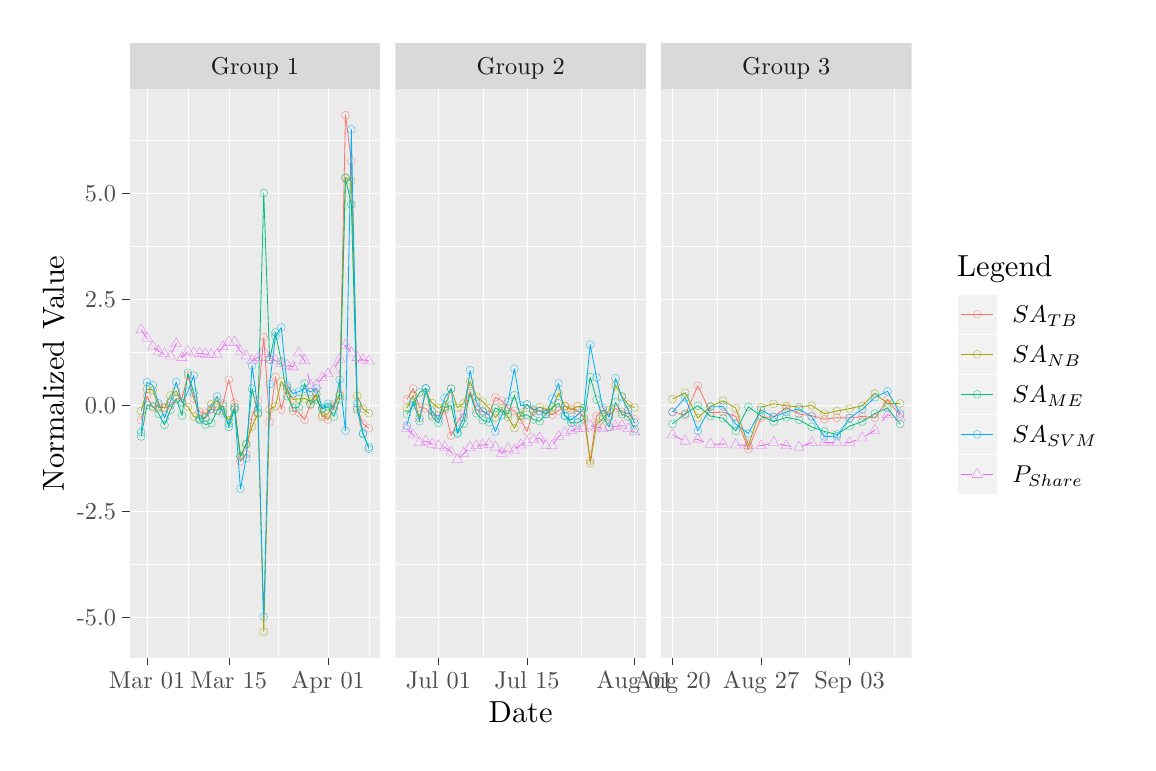
\begin{tikzpicture}[x=1pt,y=1pt]
\definecolor{fillColor}{RGB}{255,255,255}
\path[use as bounding box,fill=fillColor,fill opacity=0.00] (0,0) rectangle (397.48,258.37);
\begin{scope}
\path[clip] (  0.00,  0.00) rectangle (397.48,258.37);
\definecolor{drawColor}{RGB}{255,255,255}
\definecolor{fillColor}{RGB}{255,255,255}

\path[draw=drawColor,line width= 0.1pt,line join=round,line cap=round,fill=fillColor] (  0.00, -0.00) rectangle (397.48,258.37);
\end{scope}
\begin{scope}
\path[clip] ( 36.90, 30.73) rectangle (127.40,236.06);
\definecolor{fillColor}{gray}{0.92}

\path[fill=fillColor] ( 36.90, 30.73) rectangle (127.40,236.06);
\definecolor{drawColor}{RGB}{255,255,255}

\path[draw=drawColor,line width= 0.1pt,line join=round] ( 36.90, 64.64) --
	(127.40, 64.64);

\path[draw=drawColor,line width= 0.1pt,line join=round] ( 36.90,102.91) --
	(127.40,102.91);

\path[draw=drawColor,line width= 0.1pt,line join=round] ( 36.90,141.19) --
	(127.40,141.19);

\path[draw=drawColor,line width= 0.1pt,line join=round] ( 36.90,179.46) --
	(127.40,179.46);

\path[draw=drawColor,line width= 0.1pt,line join=round] ( 36.90,217.73) --
	(127.40,217.73);

\path[draw=drawColor,line width= 0.1pt,line join=round] ( 57.89, 30.73) --
	( 57.89,236.06);

\path[draw=drawColor,line width= 0.1pt,line join=round] ( 90.59, 30.73) --
	( 90.59,236.06);

\path[draw=drawColor,line width= 0.1pt,line join=round] (123.28, 30.73) --
	(123.28,236.06);

\path[draw=drawColor,line width= 0.1pt,line join=round] ( 36.90, 45.50) --
	(127.40, 45.50);

\path[draw=drawColor,line width= 0.1pt,line join=round] ( 36.90, 83.78) --
	(127.40, 83.78);

\path[draw=drawColor,line width= 0.1pt,line join=round] ( 36.90,122.05) --
	(127.40,122.05);

\path[draw=drawColor,line width= 0.1pt,line join=round] ( 36.90,160.32) --
	(127.40,160.32);

\path[draw=drawColor,line width= 0.1pt,line join=round] ( 36.90,198.60) --
	(127.40,198.60);

\path[draw=drawColor,line width= 0.1pt,line join=round] ( 43.12, 30.73) --
	( 43.12,236.06);

\path[draw=drawColor,line width= 0.1pt,line join=round] ( 72.66, 30.73) --
	( 72.66,236.06);

\path[draw=drawColor,line width= 0.1pt,line join=round] (108.52, 30.73) --
	(108.52,236.06);
\definecolor{drawColor}{RGB}{248,118,109}

\path[draw=drawColor,line width= 0.3pt,line join=round] ( 41.01,116.47) --
	( 43.12,125.22) --
	( 45.23,121.11) --
	( 47.34,121.83) --
	( 49.45,120.87) --
	( 51.56,121.81) --
	( 53.67,124.21) --
	( 55.78,124.56) --
	( 57.89,132.69) --
	( 60.00,124.31) --
	( 62.11,119.60) --
	( 64.22,118.95) --
	( 66.33,120.46) --
	( 68.44,120.28) --
	( 70.55,122.55) --
	( 72.66,131.14) --
	( 74.76,122.58) --
	( 76.87,101.72) --
	( 78.98,104.19) --
	( 81.09,117.98) --
	( 83.20,123.68) --
	( 85.31,146.53) --
	( 87.42,115.96) --
	( 89.53,132.24) --
	( 91.64,120.40) --
	( 93.75,128.31) --
	( 95.86,119.87) --
	( 97.97,119.33) --
	(100.08,116.71) --
	(102.19,122.12) --
	(104.30,125.85) --
	(106.41,118.46) --
	(108.52,116.73) --
	(110.63,121.64) --
	(112.73,125.69) --
	(114.84,226.73) --
	(116.95,210.07) --
	(119.06,121.00) --
	(121.17,115.23) --
	(123.28,113.61);
\definecolor{drawColor}{RGB}{163,165,0}

\path[draw=drawColor,line width= 0.3pt,line join=round] ( 41.01,119.85) --
	( 43.12,127.71) --
	( 45.23,127.41) --
	( 47.34,121.13) --
	( 49.45,121.15) --
	( 51.56,125.46) --
	( 53.67,127.03) --
	( 55.78,123.16) --
	( 57.89,121.33) --
	( 60.00,117.87) --
	( 62.11,117.18) --
	( 64.22,117.58) --
	( 66.33,122.31) --
	( 68.44,123.46) --
	( 70.55,119.86) --
	( 72.66,116.56) --
	( 74.76,121.36) --
	( 76.87,103.57) --
	( 78.98,108.02) --
	( 81.09,114.19) --
	( 83.20,118.90) --
	( 85.31, 40.06) --
	( 87.42,120.43) --
	( 89.53,121.56) --
	( 91.64,130.50) --
	( 93.75,127.64) --
	( 95.86,124.03) --
	( 97.97,124.22) --
	(100.08,124.33) --
	(102.19,123.31) --
	(104.30,126.10) --
	(106.41,117.78) --
	(108.52,118.90) --
	(110.63,122.45) --
	(112.73,125.49) --
	(114.84,204.22) --
	(116.95,203.00) --
	(119.06,125.33) --
	(121.17,120.66) --
	(123.28,119.06);
\definecolor{drawColor}{RGB}{0,191,125}

\path[draw=drawColor,line width= 0.3pt,line join=round] ( 41.01,110.67) --
	( 43.12,122.03) --
	( 45.23,121.56) --
	( 47.34,118.89) --
	( 49.45,114.85) --
	( 51.56,120.22) --
	( 53.67,124.17) --
	( 55.78,118.24) --
	( 57.89,133.59) --
	( 60.00,126.40) --
	( 62.11,116.59) --
	( 64.22,114.93) --
	( 66.33,115.52) --
	( 68.44,119.95) --
	( 70.55,121.80) --
	( 72.66,114.09) --
	( 74.76,120.42) --
	( 76.87,103.45) --
	( 78.98,107.79) --
	( 81.09,127.90) --
	( 83.20,119.21) --
	( 85.31,198.62) --
	( 87.42,138.41) --
	( 89.53,148.20) --
	( 91.64,137.77) --
	( 93.75,125.21) --
	( 95.86,120.91) --
	( 97.97,121.24) --
	(100.08,129.78) --
	(102.19,122.37) --
	(104.30,124.09) --
	(106.41,120.53) --
	(108.52,121.50) --
	(110.63,117.83) --
	(112.73,124.20) --
	(114.84,203.99) --
	(116.95,194.49) --
	(119.06,120.38) --
	(121.17,111.47) --
	(123.28,106.87);
\definecolor{drawColor}{RGB}{0,176,246}

\path[draw=drawColor,line width= 0.3pt,line join=round] ( 41.01,112.22) --
	( 43.12,130.28) --
	( 45.23,129.13) --
	( 47.34,122.56) --
	( 49.45,117.31) --
	( 51.56,123.25) --
	( 53.67,130.34) --
	( 55.78,122.64) --
	( 57.89,126.91) --
	( 60.00,132.65) --
	( 62.11,116.92) --
	( 64.22,117.25) --
	( 66.33,120.71) --
	( 68.44,125.11) --
	( 70.55,118.99) --
	( 72.66,115.19) --
	( 74.76,120.86) --
	( 76.87, 91.79) --
	( 78.98,102.83) --
	( 81.09,136.27) --
	( 83.20,120.71) --
	( 85.31, 45.55) --
	( 87.42,129.56) --
	( 89.53,146.92) --
	( 91.64,150.01) --
	( 93.75,129.03) --
	( 95.86,126.15) --
	( 97.97,126.84) --
	(100.08,127.99) --
	(102.19,126.70) --
	(104.30,128.03) --
	(106.41,120.96) --
	(108.52,122.48) --
	(110.63,120.52) --
	(112.73,131.17) --
	(114.84,112.76) --
	(116.95,221.58) --
	(119.06,122.56) --
	(121.17,111.77) --
	(123.28,106.20);
\definecolor{drawColor}{RGB}{231,107,243}

\path[draw=drawColor,line width= 0.3pt,dash pattern=on 4pt off 4pt ,line join=round] ( 41.01,149.23) --
	( 43.12,146.16) --
	( 45.23,143.09) --
	( 47.34,141.41) --
	( 49.45,140.57) --
	( 51.56,139.73) --
	( 53.67,144.20) --
	( 55.78,139.17) --
	( 57.89,141.41) --
	( 60.00,140.85) --
	( 62.11,140.57) --
	( 64.22,140.43) --
	( 66.33,140.29) --
	( 68.44,140.29) --
	( 70.55,143.09) --
	( 72.66,144.76) --
	( 74.76,144.76) --
	( 76.87,141.41) --
	( 78.98,139.73) --
	( 81.09,138.06) --
	( 83.20,139.17) --
	( 85.31,141.41) --
	( 87.42,139.17) --
	( 89.53,138.06) --
	( 91.64,136.94) --
	( 93.75,136.38) --
	( 95.86,135.82) --
	( 97.97,140.85) --
	(100.08,138.06) --
	(102.19,129.11) --
	(104.30,129.11) --
	(106.41,131.91) --
	(108.52,133.30) --
	(110.63,134.70) --
	(112.73,138.61) --
	(114.84,143.64) --
	(116.95,140.85) --
	(119.06,139.17) --
	(121.17,138.33) --
	(123.28,137.92);
\definecolor{drawColor}{RGB}{248,118,109}

\path[draw=drawColor,line width= 0.1pt,line join=round,line cap=round] ( 41.01,116.47) circle (  1.43);

\path[draw=drawColor,line width= 0.1pt,line join=round,line cap=round] ( 43.12,125.22) circle (  1.43);

\path[draw=drawColor,line width= 0.1pt,line join=round,line cap=round] ( 45.23,121.11) circle (  1.43);

\path[draw=drawColor,line width= 0.1pt,line join=round,line cap=round] ( 47.34,121.83) circle (  1.43);

\path[draw=drawColor,line width= 0.1pt,line join=round,line cap=round] ( 49.45,120.87) circle (  1.43);

\path[draw=drawColor,line width= 0.1pt,line join=round,line cap=round] ( 51.56,121.81) circle (  1.43);

\path[draw=drawColor,line width= 0.1pt,line join=round,line cap=round] ( 53.67,124.21) circle (  1.43);

\path[draw=drawColor,line width= 0.1pt,line join=round,line cap=round] ( 55.78,124.56) circle (  1.43);

\path[draw=drawColor,line width= 0.1pt,line join=round,line cap=round] ( 57.89,132.69) circle (  1.43);

\path[draw=drawColor,line width= 0.1pt,line join=round,line cap=round] ( 60.00,124.31) circle (  1.43);

\path[draw=drawColor,line width= 0.1pt,line join=round,line cap=round] ( 62.11,119.60) circle (  1.43);

\path[draw=drawColor,line width= 0.1pt,line join=round,line cap=round] ( 64.22,118.95) circle (  1.43);

\path[draw=drawColor,line width= 0.1pt,line join=round,line cap=round] ( 66.33,120.46) circle (  1.43);

\path[draw=drawColor,line width= 0.1pt,line join=round,line cap=round] ( 68.44,120.28) circle (  1.43);

\path[draw=drawColor,line width= 0.1pt,line join=round,line cap=round] ( 70.55,122.55) circle (  1.43);

\path[draw=drawColor,line width= 0.1pt,line join=round,line cap=round] ( 72.66,131.14) circle (  1.43);

\path[draw=drawColor,line width= 0.1pt,line join=round,line cap=round] ( 74.76,122.58) circle (  1.43);

\path[draw=drawColor,line width= 0.1pt,line join=round,line cap=round] ( 76.87,101.72) circle (  1.43);

\path[draw=drawColor,line width= 0.1pt,line join=round,line cap=round] ( 78.98,104.19) circle (  1.43);

\path[draw=drawColor,line width= 0.1pt,line join=round,line cap=round] ( 81.09,117.98) circle (  1.43);

\path[draw=drawColor,line width= 0.1pt,line join=round,line cap=round] ( 83.20,123.68) circle (  1.43);

\path[draw=drawColor,line width= 0.1pt,line join=round,line cap=round] ( 85.31,146.53) circle (  1.43);

\path[draw=drawColor,line width= 0.1pt,line join=round,line cap=round] ( 87.42,115.96) circle (  1.43);

\path[draw=drawColor,line width= 0.1pt,line join=round,line cap=round] ( 89.53,132.24) circle (  1.43);

\path[draw=drawColor,line width= 0.1pt,line join=round,line cap=round] ( 91.64,120.40) circle (  1.43);

\path[draw=drawColor,line width= 0.1pt,line join=round,line cap=round] ( 93.75,128.31) circle (  1.43);

\path[draw=drawColor,line width= 0.1pt,line join=round,line cap=round] ( 95.86,119.87) circle (  1.43);

\path[draw=drawColor,line width= 0.1pt,line join=round,line cap=round] ( 97.97,119.33) circle (  1.43);

\path[draw=drawColor,line width= 0.1pt,line join=round,line cap=round] (100.08,116.71) circle (  1.43);

\path[draw=drawColor,line width= 0.1pt,line join=round,line cap=round] (102.19,122.12) circle (  1.43);

\path[draw=drawColor,line width= 0.1pt,line join=round,line cap=round] (104.30,125.85) circle (  1.43);

\path[draw=drawColor,line width= 0.1pt,line join=round,line cap=round] (106.41,118.46) circle (  1.43);

\path[draw=drawColor,line width= 0.1pt,line join=round,line cap=round] (108.52,116.73) circle (  1.43);

\path[draw=drawColor,line width= 0.1pt,line join=round,line cap=round] (110.63,121.64) circle (  1.43);

\path[draw=drawColor,line width= 0.1pt,line join=round,line cap=round] (112.73,125.69) circle (  1.43);

\path[draw=drawColor,line width= 0.1pt,line join=round,line cap=round] (114.84,226.73) circle (  1.43);

\path[draw=drawColor,line width= 0.1pt,line join=round,line cap=round] (116.95,210.07) circle (  1.43);

\path[draw=drawColor,line width= 0.1pt,line join=round,line cap=round] (119.06,121.00) circle (  1.43);

\path[draw=drawColor,line width= 0.1pt,line join=round,line cap=round] (121.17,115.23) circle (  1.43);

\path[draw=drawColor,line width= 0.1pt,line join=round,line cap=round] (123.28,113.61) circle (  1.43);
\definecolor{drawColor}{RGB}{163,165,0}

\path[draw=drawColor,line width= 0.1pt,line join=round,line cap=round] ( 41.01,119.85) circle (  1.43);

\path[draw=drawColor,line width= 0.1pt,line join=round,line cap=round] ( 43.12,127.71) circle (  1.43);

\path[draw=drawColor,line width= 0.1pt,line join=round,line cap=round] ( 45.23,127.41) circle (  1.43);

\path[draw=drawColor,line width= 0.1pt,line join=round,line cap=round] ( 47.34,121.13) circle (  1.43);

\path[draw=drawColor,line width= 0.1pt,line join=round,line cap=round] ( 49.45,121.15) circle (  1.43);

\path[draw=drawColor,line width= 0.1pt,line join=round,line cap=round] ( 51.56,125.46) circle (  1.43);

\path[draw=drawColor,line width= 0.1pt,line join=round,line cap=round] ( 53.67,127.03) circle (  1.43);

\path[draw=drawColor,line width= 0.1pt,line join=round,line cap=round] ( 55.78,123.16) circle (  1.43);

\path[draw=drawColor,line width= 0.1pt,line join=round,line cap=round] ( 57.89,121.33) circle (  1.43);

\path[draw=drawColor,line width= 0.1pt,line join=round,line cap=round] ( 60.00,117.87) circle (  1.43);

\path[draw=drawColor,line width= 0.1pt,line join=round,line cap=round] ( 62.11,117.18) circle (  1.43);

\path[draw=drawColor,line width= 0.1pt,line join=round,line cap=round] ( 64.22,117.58) circle (  1.43);

\path[draw=drawColor,line width= 0.1pt,line join=round,line cap=round] ( 66.33,122.31) circle (  1.43);

\path[draw=drawColor,line width= 0.1pt,line join=round,line cap=round] ( 68.44,123.46) circle (  1.43);

\path[draw=drawColor,line width= 0.1pt,line join=round,line cap=round] ( 70.55,119.86) circle (  1.43);

\path[draw=drawColor,line width= 0.1pt,line join=round,line cap=round] ( 72.66,116.56) circle (  1.43);

\path[draw=drawColor,line width= 0.1pt,line join=round,line cap=round] ( 74.76,121.36) circle (  1.43);

\path[draw=drawColor,line width= 0.1pt,line join=round,line cap=round] ( 76.87,103.57) circle (  1.43);

\path[draw=drawColor,line width= 0.1pt,line join=round,line cap=round] ( 78.98,108.02) circle (  1.43);

\path[draw=drawColor,line width= 0.1pt,line join=round,line cap=round] ( 81.09,114.19) circle (  1.43);

\path[draw=drawColor,line width= 0.1pt,line join=round,line cap=round] ( 83.20,118.90) circle (  1.43);

\path[draw=drawColor,line width= 0.1pt,line join=round,line cap=round] ( 85.31, 40.06) circle (  1.43);

\path[draw=drawColor,line width= 0.1pt,line join=round,line cap=round] ( 87.42,120.43) circle (  1.43);

\path[draw=drawColor,line width= 0.1pt,line join=round,line cap=round] ( 89.53,121.56) circle (  1.43);

\path[draw=drawColor,line width= 0.1pt,line join=round,line cap=round] ( 91.64,130.50) circle (  1.43);

\path[draw=drawColor,line width= 0.1pt,line join=round,line cap=round] ( 93.75,127.64) circle (  1.43);

\path[draw=drawColor,line width= 0.1pt,line join=round,line cap=round] ( 95.86,124.03) circle (  1.43);

\path[draw=drawColor,line width= 0.1pt,line join=round,line cap=round] ( 97.97,124.22) circle (  1.43);

\path[draw=drawColor,line width= 0.1pt,line join=round,line cap=round] (100.08,124.33) circle (  1.43);

\path[draw=drawColor,line width= 0.1pt,line join=round,line cap=round] (102.19,123.31) circle (  1.43);

\path[draw=drawColor,line width= 0.1pt,line join=round,line cap=round] (104.30,126.10) circle (  1.43);

\path[draw=drawColor,line width= 0.1pt,line join=round,line cap=round] (106.41,117.78) circle (  1.43);

\path[draw=drawColor,line width= 0.1pt,line join=round,line cap=round] (108.52,118.90) circle (  1.43);

\path[draw=drawColor,line width= 0.1pt,line join=round,line cap=round] (110.63,122.45) circle (  1.43);

\path[draw=drawColor,line width= 0.1pt,line join=round,line cap=round] (112.73,125.49) circle (  1.43);

\path[draw=drawColor,line width= 0.1pt,line join=round,line cap=round] (114.84,204.22) circle (  1.43);

\path[draw=drawColor,line width= 0.1pt,line join=round,line cap=round] (116.95,203.00) circle (  1.43);

\path[draw=drawColor,line width= 0.1pt,line join=round,line cap=round] (119.06,125.33) circle (  1.43);

\path[draw=drawColor,line width= 0.1pt,line join=round,line cap=round] (121.17,120.66) circle (  1.43);

\path[draw=drawColor,line width= 0.1pt,line join=round,line cap=round] (123.28,119.06) circle (  1.43);
\definecolor{drawColor}{RGB}{0,191,125}

\path[draw=drawColor,line width= 0.1pt,line join=round,line cap=round] ( 41.01,110.67) circle (  1.43);

\path[draw=drawColor,line width= 0.1pt,line join=round,line cap=round] ( 43.12,122.03) circle (  1.43);

\path[draw=drawColor,line width= 0.1pt,line join=round,line cap=round] ( 45.23,121.56) circle (  1.43);

\path[draw=drawColor,line width= 0.1pt,line join=round,line cap=round] ( 47.34,118.89) circle (  1.43);

\path[draw=drawColor,line width= 0.1pt,line join=round,line cap=round] ( 49.45,114.85) circle (  1.43);

\path[draw=drawColor,line width= 0.1pt,line join=round,line cap=round] ( 51.56,120.22) circle (  1.43);

\path[draw=drawColor,line width= 0.1pt,line join=round,line cap=round] ( 53.67,124.17) circle (  1.43);

\path[draw=drawColor,line width= 0.1pt,line join=round,line cap=round] ( 55.78,118.24) circle (  1.43);

\path[draw=drawColor,line width= 0.1pt,line join=round,line cap=round] ( 57.89,133.59) circle (  1.43);

\path[draw=drawColor,line width= 0.1pt,line join=round,line cap=round] ( 60.00,126.40) circle (  1.43);

\path[draw=drawColor,line width= 0.1pt,line join=round,line cap=round] ( 62.11,116.59) circle (  1.43);

\path[draw=drawColor,line width= 0.1pt,line join=round,line cap=round] ( 64.22,114.93) circle (  1.43);

\path[draw=drawColor,line width= 0.1pt,line join=round,line cap=round] ( 66.33,115.52) circle (  1.43);

\path[draw=drawColor,line width= 0.1pt,line join=round,line cap=round] ( 68.44,119.95) circle (  1.43);

\path[draw=drawColor,line width= 0.1pt,line join=round,line cap=round] ( 70.55,121.80) circle (  1.43);

\path[draw=drawColor,line width= 0.1pt,line join=round,line cap=round] ( 72.66,114.09) circle (  1.43);

\path[draw=drawColor,line width= 0.1pt,line join=round,line cap=round] ( 74.76,120.42) circle (  1.43);

\path[draw=drawColor,line width= 0.1pt,line join=round,line cap=round] ( 76.87,103.45) circle (  1.43);

\path[draw=drawColor,line width= 0.1pt,line join=round,line cap=round] ( 78.98,107.79) circle (  1.43);

\path[draw=drawColor,line width= 0.1pt,line join=round,line cap=round] ( 81.09,127.90) circle (  1.43);

\path[draw=drawColor,line width= 0.1pt,line join=round,line cap=round] ( 83.20,119.21) circle (  1.43);

\path[draw=drawColor,line width= 0.1pt,line join=round,line cap=round] ( 85.31,198.62) circle (  1.43);

\path[draw=drawColor,line width= 0.1pt,line join=round,line cap=round] ( 87.42,138.41) circle (  1.43);

\path[draw=drawColor,line width= 0.1pt,line join=round,line cap=round] ( 89.53,148.20) circle (  1.43);

\path[draw=drawColor,line width= 0.1pt,line join=round,line cap=round] ( 91.64,137.77) circle (  1.43);

\path[draw=drawColor,line width= 0.1pt,line join=round,line cap=round] ( 93.75,125.21) circle (  1.43);

\path[draw=drawColor,line width= 0.1pt,line join=round,line cap=round] ( 95.86,120.91) circle (  1.43);

\path[draw=drawColor,line width= 0.1pt,line join=round,line cap=round] ( 97.97,121.24) circle (  1.43);

\path[draw=drawColor,line width= 0.1pt,line join=round,line cap=round] (100.08,129.78) circle (  1.43);

\path[draw=drawColor,line width= 0.1pt,line join=round,line cap=round] (102.19,122.37) circle (  1.43);

\path[draw=drawColor,line width= 0.1pt,line join=round,line cap=round] (104.30,124.09) circle (  1.43);

\path[draw=drawColor,line width= 0.1pt,line join=round,line cap=round] (106.41,120.53) circle (  1.43);

\path[draw=drawColor,line width= 0.1pt,line join=round,line cap=round] (108.52,121.50) circle (  1.43);

\path[draw=drawColor,line width= 0.1pt,line join=round,line cap=round] (110.63,117.83) circle (  1.43);

\path[draw=drawColor,line width= 0.1pt,line join=round,line cap=round] (112.73,124.20) circle (  1.43);

\path[draw=drawColor,line width= 0.1pt,line join=round,line cap=round] (114.84,203.99) circle (  1.43);

\path[draw=drawColor,line width= 0.1pt,line join=round,line cap=round] (116.95,194.49) circle (  1.43);

\path[draw=drawColor,line width= 0.1pt,line join=round,line cap=round] (119.06,120.38) circle (  1.43);

\path[draw=drawColor,line width= 0.1pt,line join=round,line cap=round] (121.17,111.47) circle (  1.43);

\path[draw=drawColor,line width= 0.1pt,line join=round,line cap=round] (123.28,106.87) circle (  1.43);
\definecolor{drawColor}{RGB}{0,176,246}

\path[draw=drawColor,line width= 0.1pt,line join=round,line cap=round] ( 41.01,112.22) circle (  1.43);

\path[draw=drawColor,line width= 0.1pt,line join=round,line cap=round] ( 43.12,130.28) circle (  1.43);

\path[draw=drawColor,line width= 0.1pt,line join=round,line cap=round] ( 45.23,129.13) circle (  1.43);

\path[draw=drawColor,line width= 0.1pt,line join=round,line cap=round] ( 47.34,122.56) circle (  1.43);

\path[draw=drawColor,line width= 0.1pt,line join=round,line cap=round] ( 49.45,117.31) circle (  1.43);

\path[draw=drawColor,line width= 0.1pt,line join=round,line cap=round] ( 51.56,123.25) circle (  1.43);

\path[draw=drawColor,line width= 0.1pt,line join=round,line cap=round] ( 53.67,130.34) circle (  1.43);

\path[draw=drawColor,line width= 0.1pt,line join=round,line cap=round] ( 55.78,122.64) circle (  1.43);

\path[draw=drawColor,line width= 0.1pt,line join=round,line cap=round] ( 57.89,126.91) circle (  1.43);

\path[draw=drawColor,line width= 0.1pt,line join=round,line cap=round] ( 60.00,132.65) circle (  1.43);

\path[draw=drawColor,line width= 0.1pt,line join=round,line cap=round] ( 62.11,116.92) circle (  1.43);

\path[draw=drawColor,line width= 0.1pt,line join=round,line cap=round] ( 64.22,117.25) circle (  1.43);

\path[draw=drawColor,line width= 0.1pt,line join=round,line cap=round] ( 66.33,120.71) circle (  1.43);

\path[draw=drawColor,line width= 0.1pt,line join=round,line cap=round] ( 68.44,125.11) circle (  1.43);

\path[draw=drawColor,line width= 0.1pt,line join=round,line cap=round] ( 70.55,118.99) circle (  1.43);

\path[draw=drawColor,line width= 0.1pt,line join=round,line cap=round] ( 72.66,115.19) circle (  1.43);

\path[draw=drawColor,line width= 0.1pt,line join=round,line cap=round] ( 74.76,120.86) circle (  1.43);

\path[draw=drawColor,line width= 0.1pt,line join=round,line cap=round] ( 76.87, 91.79) circle (  1.43);

\path[draw=drawColor,line width= 0.1pt,line join=round,line cap=round] ( 78.98,102.83) circle (  1.43);

\path[draw=drawColor,line width= 0.1pt,line join=round,line cap=round] ( 81.09,136.27) circle (  1.43);

\path[draw=drawColor,line width= 0.1pt,line join=round,line cap=round] ( 83.20,120.71) circle (  1.43);

\path[draw=drawColor,line width= 0.1pt,line join=round,line cap=round] ( 85.31, 45.55) circle (  1.43);

\path[draw=drawColor,line width= 0.1pt,line join=round,line cap=round] ( 87.42,129.56) circle (  1.43);

\path[draw=drawColor,line width= 0.1pt,line join=round,line cap=round] ( 89.53,146.92) circle (  1.43);

\path[draw=drawColor,line width= 0.1pt,line join=round,line cap=round] ( 91.64,150.01) circle (  1.43);

\path[draw=drawColor,line width= 0.1pt,line join=round,line cap=round] ( 93.75,129.03) circle (  1.43);

\path[draw=drawColor,line width= 0.1pt,line join=round,line cap=round] ( 95.86,126.15) circle (  1.43);

\path[draw=drawColor,line width= 0.1pt,line join=round,line cap=round] ( 97.97,126.84) circle (  1.43);

\path[draw=drawColor,line width= 0.1pt,line join=round,line cap=round] (100.08,127.99) circle (  1.43);

\path[draw=drawColor,line width= 0.1pt,line join=round,line cap=round] (102.19,126.70) circle (  1.43);

\path[draw=drawColor,line width= 0.1pt,line join=round,line cap=round] (104.30,128.03) circle (  1.43);

\path[draw=drawColor,line width= 0.1pt,line join=round,line cap=round] (106.41,120.96) circle (  1.43);

\path[draw=drawColor,line width= 0.1pt,line join=round,line cap=round] (108.52,122.48) circle (  1.43);

\path[draw=drawColor,line width= 0.1pt,line join=round,line cap=round] (110.63,120.52) circle (  1.43);

\path[draw=drawColor,line width= 0.1pt,line join=round,line cap=round] (112.73,131.17) circle (  1.43);

\path[draw=drawColor,line width= 0.1pt,line join=round,line cap=round] (114.84,112.76) circle (  1.43);

\path[draw=drawColor,line width= 0.1pt,line join=round,line cap=round] (116.95,221.58) circle (  1.43);

\path[draw=drawColor,line width= 0.1pt,line join=round,line cap=round] (119.06,122.56) circle (  1.43);

\path[draw=drawColor,line width= 0.1pt,line join=round,line cap=round] (121.17,111.77) circle (  1.43);

\path[draw=drawColor,line width= 0.1pt,line join=round,line cap=round] (123.28,106.20) circle (  1.43);
\definecolor{drawColor}{RGB}{231,107,243}

\path[draw=drawColor,line width= 0.1pt,line join=round,line cap=round] ( 41.01,151.45) --
	( 42.93,148.13) --
	( 39.09,148.13) --
	( 41.01,151.45);

\path[draw=drawColor,line width= 0.1pt,line join=round,line cap=round] ( 43.12,148.38) --
	( 45.04,145.05) --
	( 41.20,145.05) --
	( 43.12,148.38);

\path[draw=drawColor,line width= 0.1pt,line join=round,line cap=round] ( 45.23,145.30) --
	( 47.15,141.98) --
	( 43.31,141.98) --
	( 45.23,145.30);

\path[draw=drawColor,line width= 0.1pt,line join=round,line cap=round] ( 47.34,143.63) --
	( 49.26,140.30) --
	( 45.42,140.30) --
	( 47.34,143.63);

\path[draw=drawColor,line width= 0.1pt,line join=round,line cap=round] ( 49.45,142.79) --
	( 51.37,139.46) --
	( 47.53,139.46) --
	( 49.45,142.79);

\path[draw=drawColor,line width= 0.1pt,line join=round,line cap=round] ( 51.56,141.95) --
	( 53.48,138.62) --
	( 49.64,138.62) --
	( 51.56,141.95);

\path[draw=drawColor,line width= 0.1pt,line join=round,line cap=round] ( 53.67,146.42) --
	( 55.59,143.09) --
	( 51.75,143.09) --
	( 53.67,146.42);

\path[draw=drawColor,line width= 0.1pt,line join=round,line cap=round] ( 55.78,141.39) --
	( 57.70,138.06) --
	( 53.86,138.06) --
	( 55.78,141.39);

\path[draw=drawColor,line width= 0.1pt,line join=round,line cap=round] ( 57.89,143.63) --
	( 59.81,140.30) --
	( 55.97,140.30) --
	( 57.89,143.63);

\path[draw=drawColor,line width= 0.1pt,line join=round,line cap=round] ( 60.00,143.07) --
	( 61.92,139.74) --
	( 58.08,139.74) --
	( 60.00,143.07);

\path[draw=drawColor,line width= 0.1pt,line join=round,line cap=round] ( 62.11,142.79) --
	( 64.03,139.46) --
	( 60.19,139.46) --
	( 62.11,142.79);

\path[draw=drawColor,line width= 0.1pt,line join=round,line cap=round] ( 64.22,142.65) --
	( 66.14,139.32) --
	( 62.30,139.32) --
	( 64.22,142.65);

\path[draw=drawColor,line width= 0.1pt,line join=round,line cap=round] ( 66.33,142.51) --
	( 68.25,139.18) --
	( 64.41,139.18) --
	( 66.33,142.51);

\path[draw=drawColor,line width= 0.1pt,line join=round,line cap=round] ( 68.44,142.51) --
	( 70.36,139.18) --
	( 66.51,139.18) --
	( 68.44,142.51);

\path[draw=drawColor,line width= 0.1pt,line join=round,line cap=round] ( 70.55,145.30) --
	( 72.47,141.98) --
	( 68.62,141.98) --
	( 70.55,145.30);

\path[draw=drawColor,line width= 0.1pt,line join=round,line cap=round] ( 72.66,146.98) --
	( 74.58,143.65) --
	( 70.73,143.65) --
	( 72.66,146.98);

\path[draw=drawColor,line width= 0.1pt,line join=round,line cap=round] ( 74.76,146.98) --
	( 76.69,143.65) --
	( 72.84,143.65) --
	( 74.76,146.98);

\path[draw=drawColor,line width= 0.1pt,line join=round,line cap=round] ( 76.87,143.63) --
	( 78.80,140.30) --
	( 74.95,140.30) --
	( 76.87,143.63);

\path[draw=drawColor,line width= 0.1pt,line join=round,line cap=round] ( 78.98,141.95) --
	( 80.90,138.62) --
	( 77.06,138.62) --
	( 78.98,141.95);

\path[draw=drawColor,line width= 0.1pt,line join=round,line cap=round] ( 81.09,140.27) --
	( 83.01,136.95) --
	( 79.17,136.95) --
	( 81.09,140.27);

\path[draw=drawColor,line width= 0.1pt,line join=round,line cap=round] ( 83.20,141.39) --
	( 85.12,138.06) --
	( 81.28,138.06) --
	( 83.20,141.39);

\path[draw=drawColor,line width= 0.1pt,line join=round,line cap=round] ( 85.31,143.63) --
	( 87.23,140.30) --
	( 83.39,140.30) --
	( 85.31,143.63);

\path[draw=drawColor,line width= 0.1pt,line join=round,line cap=round] ( 87.42,141.39) --
	( 89.34,138.06) --
	( 85.50,138.06) --
	( 87.42,141.39);

\path[draw=drawColor,line width= 0.1pt,line join=round,line cap=round] ( 89.53,140.27) --
	( 91.45,136.95) --
	( 87.61,136.95) --
	( 89.53,140.27);

\path[draw=drawColor,line width= 0.1pt,line join=round,line cap=round] ( 91.64,139.16) --
	( 93.56,135.83) --
	( 89.72,135.83) --
	( 91.64,139.16);

\path[draw=drawColor,line width= 0.1pt,line join=round,line cap=round] ( 93.75,138.60) --
	( 95.67,135.27) --
	( 91.83,135.27) --
	( 93.75,138.60);

\path[draw=drawColor,line width= 0.1pt,line join=round,line cap=round] ( 95.86,138.04) --
	( 97.78,134.71) --
	( 93.94,134.71) --
	( 95.86,138.04);

\path[draw=drawColor,line width= 0.1pt,line join=round,line cap=round] ( 97.97,143.07) --
	( 99.89,139.74) --
	( 96.05,139.74) --
	( 97.97,143.07);

\path[draw=drawColor,line width= 0.1pt,line join=round,line cap=round] (100.08,140.27) --
	(102.00,136.95) --
	( 98.16,136.95) --
	(100.08,140.27);

\path[draw=drawColor,line width= 0.1pt,line join=round,line cap=round] (102.19,131.33) --
	(104.11,128.00) --
	(100.27,128.00) --
	(102.19,131.33);

\path[draw=drawColor,line width= 0.1pt,line join=round,line cap=round] (104.30,131.33) --
	(106.22,128.00) --
	(102.38,128.00) --
	(104.30,131.33);

\path[draw=drawColor,line width= 0.1pt,line join=round,line cap=round] (106.41,134.12) --
	(108.33,130.80) --
	(104.49,130.80) --
	(106.41,134.12);

\path[draw=drawColor,line width= 0.1pt,line join=round,line cap=round] (108.52,135.52) --
	(110.44,132.19) --
	(106.59,132.19) --
	(108.52,135.52);

\path[draw=drawColor,line width= 0.1pt,line join=round,line cap=round] (110.63,136.92) --
	(112.55,133.59) --
	(108.70,133.59) --
	(110.63,136.92);

\path[draw=drawColor,line width= 0.1pt,line join=round,line cap=round] (112.73,140.83) --
	(114.66,137.50) --
	(110.81,137.50) --
	(112.73,140.83);

\path[draw=drawColor,line width= 0.1pt,line join=round,line cap=round] (114.84,145.86) --
	(116.77,142.54) --
	(112.92,142.54) --
	(114.84,145.86);

\path[draw=drawColor,line width= 0.1pt,line join=round,line cap=round] (116.95,143.07) --
	(118.88,139.74) --
	(115.03,139.74) --
	(116.95,143.07);

\path[draw=drawColor,line width= 0.1pt,line join=round,line cap=round] (119.06,141.39) --
	(120.98,138.06) --
	(117.14,138.06) --
	(119.06,141.39);

\path[draw=drawColor,line width= 0.1pt,line join=round,line cap=round] (121.17,140.55) --
	(123.09,137.23) --
	(119.25,137.23) --
	(121.17,140.55);

\path[draw=drawColor,line width= 0.1pt,line join=round,line cap=round] (123.28,140.13) --
	(125.20,136.81) --
	(121.36,136.81) --
	(123.28,140.13);
\end{scope}
\begin{scope}
\path[clip] (132.90, 30.73) rectangle (223.39,236.06);
\definecolor{fillColor}{gray}{0.92}

\path[fill=fillColor] (132.90, 30.73) rectangle (223.39,236.06);
\definecolor{drawColor}{RGB}{255,255,255}

\path[draw=drawColor,line width= 0.1pt,line join=round] (132.90, 64.64) --
	(223.39, 64.64);

\path[draw=drawColor,line width= 0.1pt,line join=round] (132.90,102.91) --
	(223.39,102.91);

\path[draw=drawColor,line width= 0.1pt,line join=round] (132.90,141.19) --
	(223.39,141.19);

\path[draw=drawColor,line width= 0.1pt,line join=round] (132.90,179.46) --
	(223.39,179.46);

\path[draw=drawColor,line width= 0.1pt,line join=round] (132.90,217.73) --
	(223.39,217.73);

\path[draw=drawColor,line width= 0.1pt,line join=round] (164.43, 30.73) --
	(164.43,236.06);

\path[draw=drawColor,line width= 0.1pt,line join=round] (199.85, 30.73) --
	(199.85,236.06);

\path[draw=drawColor,line width= 0.1pt,line join=round] (132.90, 45.50) --
	(223.39, 45.50);

\path[draw=drawColor,line width= 0.1pt,line join=round] (132.90, 83.78) --
	(223.39, 83.78);

\path[draw=drawColor,line width= 0.1pt,line join=round] (132.90,122.05) --
	(223.39,122.05);

\path[draw=drawColor,line width= 0.1pt,line join=round] (132.90,160.32) --
	(223.39,160.32);

\path[draw=drawColor,line width= 0.1pt,line join=round] (132.90,198.60) --
	(223.39,198.60);

\path[draw=drawColor,line width= 0.1pt,line join=round] (148.44, 30.73) --
	(148.44,236.06);

\path[draw=drawColor,line width= 0.1pt,line join=round] (180.43, 30.73) --
	(180.43,236.06);

\path[draw=drawColor,line width= 0.1pt,line join=round] (219.28, 30.73) --
	(219.28,236.06);
\definecolor{drawColor}{RGB}{248,118,109}

\path[draw=drawColor,line width= 0.3pt,line join=round] (137.01,124.01) --
	(139.29,127.93) --
	(141.58,121.19) --
	(143.86,120.79) --
	(146.15,118.44) --
	(148.44,118.07) --
	(150.72,120.24) --
	(153.01,110.94) --
	(155.29,115.89) --
	(157.58,118.74) --
	(159.86,127.07) --
	(162.15,120.34) --
	(164.43,119.55) --
	(166.72,118.65) --
	(169.00,124.78) --
	(171.29,123.58) --
	(173.57,120.78) --
	(175.86,119.91) --
	(178.14,116.76) --
	(180.43,112.49) --
	(182.71,119.70) --
	(185.00,119.94) --
	(187.28,119.41) --
	(189.57,118.51) --
	(191.86,120.02) --
	(194.14,121.66) --
	(196.43,120.79) --
	(198.71,119.87) --
	(201.00,117.65) --
	(203.28,101.90) --
	(205.57,118.07) --
	(207.85,120.22) --
	(210.14,118.11) --
	(212.42,120.79) --
	(214.71,119.56) --
	(216.99,118.88) --
	(219.28,116.88);
\definecolor{drawColor}{RGB}{163,165,0}

\path[draw=drawColor,line width= 0.3pt,line join=round] (137.01,120.96) --
	(139.29,125.47) --
	(141.58,117.22) --
	(143.86,126.57) --
	(146.15,122.74) --
	(148.44,120.85) --
	(150.72,121.54) --
	(153.01,127.89) --
	(155.29,121.07) --
	(157.58,122.54) --
	(159.86,130.50) --
	(162.15,125.03) --
	(164.43,123.25) --
	(166.72,120.85) --
	(169.00,117.47) --
	(171.29,120.72) --
	(173.57,117.71) --
	(175.86,113.63) --
	(178.14,118.32) --
	(180.43,122.21) --
	(182.71,120.05) --
	(185.00,121.27) --
	(187.28,120.38) --
	(189.57,120.36) --
	(191.86,126.29) --
	(194.14,121.69) --
	(196.43,120.19) --
	(198.71,121.60) --
	(201.00,121.00) --
	(203.28,100.98) --
	(205.57,115.00) --
	(207.85,117.07) --
	(210.14,120.26) --
	(212.42,129.24) --
	(214.71,125.22) --
	(216.99,122.18) --
	(219.28,121.09);
\definecolor{drawColor}{RGB}{0,191,125}

\path[draw=drawColor,line width= 0.3pt,line join=round] (137.01,118.69) --
	(139.29,121.92) --
	(141.58,126.55) --
	(143.86,128.03) --
	(146.15,117.86) --
	(148.44,115.58) --
	(150.72,121.06) --
	(153.01,121.83) --
	(155.29,111.65) --
	(157.58,115.20) --
	(159.86,126.38) --
	(162.15,119.02) --
	(164.43,116.50) --
	(166.72,115.78) --
	(169.00,120.94) --
	(171.29,119.80) --
	(173.57,118.74) --
	(175.86,125.54) --
	(178.14,117.96) --
	(180.43,118.51) --
	(182.71,116.79) --
	(185.00,116.14) --
	(187.28,118.68) --
	(189.57,121.17) --
	(191.86,122.64) --
	(194.14,118.04) --
	(196.43,115.61) --
	(198.71,115.60) --
	(201.00,116.94) --
	(203.28,132.13) --
	(205.57,124.01) --
	(207.85,117.75) --
	(210.14,114.09) --
	(212.42,122.99) --
	(214.71,118.71) --
	(216.99,117.84) --
	(219.28,113.27);
\definecolor{drawColor}{RGB}{0,176,246}

\path[draw=drawColor,line width= 0.3pt,line join=round] (137.01,114.57) --
	(139.29,123.29) --
	(141.58,116.15) --
	(143.86,128.07) --
	(146.15,119.63) --
	(148.44,116.94) --
	(150.72,124.60) --
	(153.01,127.94) --
	(155.29,112.16) --
	(157.58,117.59) --
	(159.86,134.58) --
	(162.15,122.94) --
	(164.43,119.83) --
	(166.72,118.33) --
	(169.00,112.43) --
	(171.29,118.28) --
	(173.57,123.26) --
	(175.86,135.14) --
	(178.14,121.80) --
	(180.43,122.19) --
	(182.71,120.51) --
	(185.00,119.77) --
	(187.28,118.78) --
	(189.57,124.33) --
	(191.86,129.83) --
	(194.14,118.19) --
	(196.43,116.64) --
	(198.71,118.43) --
	(201.00,120.84) --
	(203.28,143.84) --
	(205.57,131.96) --
	(207.85,121.02) --
	(210.14,117.60) --
	(212.42,131.71) --
	(214.71,124.81) --
	(216.99,120.20) --
	(219.28,115.56);
\definecolor{drawColor}{RGB}{231,107,243}

\path[draw=drawColor,line width= 0.3pt,dash pattern=on 4pt off 4pt ,line join=round] (137.01,113.46) --
	(139.29,111.22) --
	(141.58,108.43) --
	(143.86,108.99) --
	(146.15,107.87) --
	(148.44,107.31) --
	(150.72,106.75) --
	(153.01,105.08) --
	(155.29,102.28) --
	(157.58,104.52) --
	(159.86,106.75) --
	(162.15,107.31) --
	(164.43,107.59) --
	(166.72,107.87) --
	(169.00,106.75) --
	(171.29,104.52) --
	(173.57,106.19) --
	(175.86,105.63) --
	(178.14,107.59) --
	(180.43,108.57) --
	(182.71,109.55) --
	(185.00,110.11) --
	(187.28,107.31) --
	(189.57,107.31) --
	(191.86,110.67) --
	(194.14,112.06) --
	(196.43,112.76) --
	(198.71,113.46) --
	(201.00,113.46) --
	(203.28,114.58) --
	(205.57,114.02) --
	(207.85,113.46) --
	(210.14,114.02) --
	(212.42,114.30) --
	(214.71,114.58) --
	(216.99,113.46) --
	(219.28,112.34);
\definecolor{drawColor}{RGB}{248,118,109}

\path[draw=drawColor,line width= 0.1pt,line join=round,line cap=round] (137.01,124.01) circle (  1.43);

\path[draw=drawColor,line width= 0.1pt,line join=round,line cap=round] (139.29,127.93) circle (  1.43);

\path[draw=drawColor,line width= 0.1pt,line join=round,line cap=round] (141.58,121.19) circle (  1.43);

\path[draw=drawColor,line width= 0.1pt,line join=round,line cap=round] (143.86,120.79) circle (  1.43);

\path[draw=drawColor,line width= 0.1pt,line join=round,line cap=round] (146.15,118.44) circle (  1.43);

\path[draw=drawColor,line width= 0.1pt,line join=round,line cap=round] (148.44,118.07) circle (  1.43);

\path[draw=drawColor,line width= 0.1pt,line join=round,line cap=round] (150.72,120.24) circle (  1.43);

\path[draw=drawColor,line width= 0.1pt,line join=round,line cap=round] (153.01,110.94) circle (  1.43);

\path[draw=drawColor,line width= 0.1pt,line join=round,line cap=round] (155.29,115.89) circle (  1.43);

\path[draw=drawColor,line width= 0.1pt,line join=round,line cap=round] (157.58,118.74) circle (  1.43);

\path[draw=drawColor,line width= 0.1pt,line join=round,line cap=round] (159.86,127.07) circle (  1.43);

\path[draw=drawColor,line width= 0.1pt,line join=round,line cap=round] (162.15,120.34) circle (  1.43);

\path[draw=drawColor,line width= 0.1pt,line join=round,line cap=round] (164.43,119.55) circle (  1.43);

\path[draw=drawColor,line width= 0.1pt,line join=round,line cap=round] (166.72,118.65) circle (  1.43);

\path[draw=drawColor,line width= 0.1pt,line join=round,line cap=round] (169.00,124.78) circle (  1.43);

\path[draw=drawColor,line width= 0.1pt,line join=round,line cap=round] (171.29,123.58) circle (  1.43);

\path[draw=drawColor,line width= 0.1pt,line join=round,line cap=round] (173.57,120.78) circle (  1.43);

\path[draw=drawColor,line width= 0.1pt,line join=round,line cap=round] (175.86,119.91) circle (  1.43);

\path[draw=drawColor,line width= 0.1pt,line join=round,line cap=round] (178.14,116.76) circle (  1.43);

\path[draw=drawColor,line width= 0.1pt,line join=round,line cap=round] (180.43,112.49) circle (  1.43);

\path[draw=drawColor,line width= 0.1pt,line join=round,line cap=round] (182.71,119.70) circle (  1.43);

\path[draw=drawColor,line width= 0.1pt,line join=round,line cap=round] (185.00,119.94) circle (  1.43);

\path[draw=drawColor,line width= 0.1pt,line join=round,line cap=round] (187.28,119.41) circle (  1.43);

\path[draw=drawColor,line width= 0.1pt,line join=round,line cap=round] (189.57,118.51) circle (  1.43);

\path[draw=drawColor,line width= 0.1pt,line join=round,line cap=round] (191.86,120.02) circle (  1.43);

\path[draw=drawColor,line width= 0.1pt,line join=round,line cap=round] (194.14,121.66) circle (  1.43);

\path[draw=drawColor,line width= 0.1pt,line join=round,line cap=round] (196.43,120.79) circle (  1.43);

\path[draw=drawColor,line width= 0.1pt,line join=round,line cap=round] (198.71,119.87) circle (  1.43);

\path[draw=drawColor,line width= 0.1pt,line join=round,line cap=round] (201.00,117.65) circle (  1.43);

\path[draw=drawColor,line width= 0.1pt,line join=round,line cap=round] (203.28,101.90) circle (  1.43);

\path[draw=drawColor,line width= 0.1pt,line join=round,line cap=round] (205.57,118.07) circle (  1.43);

\path[draw=drawColor,line width= 0.1pt,line join=round,line cap=round] (207.85,120.22) circle (  1.43);

\path[draw=drawColor,line width= 0.1pt,line join=round,line cap=round] (210.14,118.11) circle (  1.43);

\path[draw=drawColor,line width= 0.1pt,line join=round,line cap=round] (212.42,120.79) circle (  1.43);

\path[draw=drawColor,line width= 0.1pt,line join=round,line cap=round] (214.71,119.56) circle (  1.43);

\path[draw=drawColor,line width= 0.1pt,line join=round,line cap=round] (216.99,118.88) circle (  1.43);

\path[draw=drawColor,line width= 0.1pt,line join=round,line cap=round] (219.28,116.88) circle (  1.43);
\definecolor{drawColor}{RGB}{163,165,0}

\path[draw=drawColor,line width= 0.1pt,line join=round,line cap=round] (137.01,120.96) circle (  1.43);

\path[draw=drawColor,line width= 0.1pt,line join=round,line cap=round] (139.29,125.47) circle (  1.43);

\path[draw=drawColor,line width= 0.1pt,line join=round,line cap=round] (141.58,117.22) circle (  1.43);

\path[draw=drawColor,line width= 0.1pt,line join=round,line cap=round] (143.86,126.57) circle (  1.43);

\path[draw=drawColor,line width= 0.1pt,line join=round,line cap=round] (146.15,122.74) circle (  1.43);

\path[draw=drawColor,line width= 0.1pt,line join=round,line cap=round] (148.44,120.85) circle (  1.43);

\path[draw=drawColor,line width= 0.1pt,line join=round,line cap=round] (150.72,121.54) circle (  1.43);

\path[draw=drawColor,line width= 0.1pt,line join=round,line cap=round] (153.01,127.89) circle (  1.43);

\path[draw=drawColor,line width= 0.1pt,line join=round,line cap=round] (155.29,121.07) circle (  1.43);

\path[draw=drawColor,line width= 0.1pt,line join=round,line cap=round] (157.58,122.54) circle (  1.43);

\path[draw=drawColor,line width= 0.1pt,line join=round,line cap=round] (159.86,130.50) circle (  1.43);

\path[draw=drawColor,line width= 0.1pt,line join=round,line cap=round] (162.15,125.03) circle (  1.43);

\path[draw=drawColor,line width= 0.1pt,line join=round,line cap=round] (164.43,123.25) circle (  1.43);

\path[draw=drawColor,line width= 0.1pt,line join=round,line cap=round] (166.72,120.85) circle (  1.43);

\path[draw=drawColor,line width= 0.1pt,line join=round,line cap=round] (169.00,117.47) circle (  1.43);

\path[draw=drawColor,line width= 0.1pt,line join=round,line cap=round] (171.29,120.72) circle (  1.43);

\path[draw=drawColor,line width= 0.1pt,line join=round,line cap=round] (173.57,117.71) circle (  1.43);

\path[draw=drawColor,line width= 0.1pt,line join=round,line cap=round] (175.86,113.63) circle (  1.43);

\path[draw=drawColor,line width= 0.1pt,line join=round,line cap=round] (178.14,118.32) circle (  1.43);

\path[draw=drawColor,line width= 0.1pt,line join=round,line cap=round] (180.43,122.21) circle (  1.43);

\path[draw=drawColor,line width= 0.1pt,line join=round,line cap=round] (182.71,120.05) circle (  1.43);

\path[draw=drawColor,line width= 0.1pt,line join=round,line cap=round] (185.00,121.27) circle (  1.43);

\path[draw=drawColor,line width= 0.1pt,line join=round,line cap=round] (187.28,120.38) circle (  1.43);

\path[draw=drawColor,line width= 0.1pt,line join=round,line cap=round] (189.57,120.36) circle (  1.43);

\path[draw=drawColor,line width= 0.1pt,line join=round,line cap=round] (191.86,126.29) circle (  1.43);

\path[draw=drawColor,line width= 0.1pt,line join=round,line cap=round] (194.14,121.69) circle (  1.43);

\path[draw=drawColor,line width= 0.1pt,line join=round,line cap=round] (196.43,120.19) circle (  1.43);

\path[draw=drawColor,line width= 0.1pt,line join=round,line cap=round] (198.71,121.60) circle (  1.43);

\path[draw=drawColor,line width= 0.1pt,line join=round,line cap=round] (201.00,121.00) circle (  1.43);

\path[draw=drawColor,line width= 0.1pt,line join=round,line cap=round] (203.28,100.98) circle (  1.43);

\path[draw=drawColor,line width= 0.1pt,line join=round,line cap=round] (205.57,115.00) circle (  1.43);

\path[draw=drawColor,line width= 0.1pt,line join=round,line cap=round] (207.85,117.07) circle (  1.43);

\path[draw=drawColor,line width= 0.1pt,line join=round,line cap=round] (210.14,120.26) circle (  1.43);

\path[draw=drawColor,line width= 0.1pt,line join=round,line cap=round] (212.42,129.24) circle (  1.43);

\path[draw=drawColor,line width= 0.1pt,line join=round,line cap=round] (214.71,125.22) circle (  1.43);

\path[draw=drawColor,line width= 0.1pt,line join=round,line cap=round] (216.99,122.18) circle (  1.43);

\path[draw=drawColor,line width= 0.1pt,line join=round,line cap=round] (219.28,121.09) circle (  1.43);
\definecolor{drawColor}{RGB}{0,191,125}

\path[draw=drawColor,line width= 0.1pt,line join=round,line cap=round] (137.01,118.69) circle (  1.43);

\path[draw=drawColor,line width= 0.1pt,line join=round,line cap=round] (139.29,121.92) circle (  1.43);

\path[draw=drawColor,line width= 0.1pt,line join=round,line cap=round] (141.58,126.55) circle (  1.43);

\path[draw=drawColor,line width= 0.1pt,line join=round,line cap=round] (143.86,128.03) circle (  1.43);

\path[draw=drawColor,line width= 0.1pt,line join=round,line cap=round] (146.15,117.86) circle (  1.43);

\path[draw=drawColor,line width= 0.1pt,line join=round,line cap=round] (148.44,115.58) circle (  1.43);

\path[draw=drawColor,line width= 0.1pt,line join=round,line cap=round] (150.72,121.06) circle (  1.43);

\path[draw=drawColor,line width= 0.1pt,line join=round,line cap=round] (153.01,121.83) circle (  1.43);

\path[draw=drawColor,line width= 0.1pt,line join=round,line cap=round] (155.29,111.65) circle (  1.43);

\path[draw=drawColor,line width= 0.1pt,line join=round,line cap=round] (157.58,115.20) circle (  1.43);

\path[draw=drawColor,line width= 0.1pt,line join=round,line cap=round] (159.86,126.38) circle (  1.43);

\path[draw=drawColor,line width= 0.1pt,line join=round,line cap=round] (162.15,119.02) circle (  1.43);

\path[draw=drawColor,line width= 0.1pt,line join=round,line cap=round] (164.43,116.50) circle (  1.43);

\path[draw=drawColor,line width= 0.1pt,line join=round,line cap=round] (166.72,115.78) circle (  1.43);

\path[draw=drawColor,line width= 0.1pt,line join=round,line cap=round] (169.00,120.94) circle (  1.43);

\path[draw=drawColor,line width= 0.1pt,line join=round,line cap=round] (171.29,119.80) circle (  1.43);

\path[draw=drawColor,line width= 0.1pt,line join=round,line cap=round] (173.57,118.74) circle (  1.43);

\path[draw=drawColor,line width= 0.1pt,line join=round,line cap=round] (175.86,125.54) circle (  1.43);

\path[draw=drawColor,line width= 0.1pt,line join=round,line cap=round] (178.14,117.96) circle (  1.43);

\path[draw=drawColor,line width= 0.1pt,line join=round,line cap=round] (180.43,118.51) circle (  1.43);

\path[draw=drawColor,line width= 0.1pt,line join=round,line cap=round] (182.71,116.79) circle (  1.43);

\path[draw=drawColor,line width= 0.1pt,line join=round,line cap=round] (185.00,116.14) circle (  1.43);

\path[draw=drawColor,line width= 0.1pt,line join=round,line cap=round] (187.28,118.68) circle (  1.43);

\path[draw=drawColor,line width= 0.1pt,line join=round,line cap=round] (189.57,121.17) circle (  1.43);

\path[draw=drawColor,line width= 0.1pt,line join=round,line cap=round] (191.86,122.64) circle (  1.43);

\path[draw=drawColor,line width= 0.1pt,line join=round,line cap=round] (194.14,118.04) circle (  1.43);

\path[draw=drawColor,line width= 0.1pt,line join=round,line cap=round] (196.43,115.61) circle (  1.43);

\path[draw=drawColor,line width= 0.1pt,line join=round,line cap=round] (198.71,115.60) circle (  1.43);

\path[draw=drawColor,line width= 0.1pt,line join=round,line cap=round] (201.00,116.94) circle (  1.43);

\path[draw=drawColor,line width= 0.1pt,line join=round,line cap=round] (203.28,132.13) circle (  1.43);

\path[draw=drawColor,line width= 0.1pt,line join=round,line cap=round] (205.57,124.01) circle (  1.43);

\path[draw=drawColor,line width= 0.1pt,line join=round,line cap=round] (207.85,117.75) circle (  1.43);

\path[draw=drawColor,line width= 0.1pt,line join=round,line cap=round] (210.14,114.09) circle (  1.43);

\path[draw=drawColor,line width= 0.1pt,line join=round,line cap=round] (212.42,122.99) circle (  1.43);

\path[draw=drawColor,line width= 0.1pt,line join=round,line cap=round] (214.71,118.71) circle (  1.43);

\path[draw=drawColor,line width= 0.1pt,line join=round,line cap=round] (216.99,117.84) circle (  1.43);

\path[draw=drawColor,line width= 0.1pt,line join=round,line cap=round] (219.28,113.27) circle (  1.43);
\definecolor{drawColor}{RGB}{0,176,246}

\path[draw=drawColor,line width= 0.1pt,line join=round,line cap=round] (137.01,114.57) circle (  1.43);

\path[draw=drawColor,line width= 0.1pt,line join=round,line cap=round] (139.29,123.29) circle (  1.43);

\path[draw=drawColor,line width= 0.1pt,line join=round,line cap=round] (141.58,116.15) circle (  1.43);

\path[draw=drawColor,line width= 0.1pt,line join=round,line cap=round] (143.86,128.07) circle (  1.43);

\path[draw=drawColor,line width= 0.1pt,line join=round,line cap=round] (146.15,119.63) circle (  1.43);

\path[draw=drawColor,line width= 0.1pt,line join=round,line cap=round] (148.44,116.94) circle (  1.43);

\path[draw=drawColor,line width= 0.1pt,line join=round,line cap=round] (150.72,124.60) circle (  1.43);

\path[draw=drawColor,line width= 0.1pt,line join=round,line cap=round] (153.01,127.94) circle (  1.43);

\path[draw=drawColor,line width= 0.1pt,line join=round,line cap=round] (155.29,112.16) circle (  1.43);

\path[draw=drawColor,line width= 0.1pt,line join=round,line cap=round] (157.58,117.59) circle (  1.43);

\path[draw=drawColor,line width= 0.1pt,line join=round,line cap=round] (159.86,134.58) circle (  1.43);

\path[draw=drawColor,line width= 0.1pt,line join=round,line cap=round] (162.15,122.94) circle (  1.43);

\path[draw=drawColor,line width= 0.1pt,line join=round,line cap=round] (164.43,119.83) circle (  1.43);

\path[draw=drawColor,line width= 0.1pt,line join=round,line cap=round] (166.72,118.33) circle (  1.43);

\path[draw=drawColor,line width= 0.1pt,line join=round,line cap=round] (169.00,112.43) circle (  1.43);

\path[draw=drawColor,line width= 0.1pt,line join=round,line cap=round] (171.29,118.28) circle (  1.43);

\path[draw=drawColor,line width= 0.1pt,line join=round,line cap=round] (173.57,123.26) circle (  1.43);

\path[draw=drawColor,line width= 0.1pt,line join=round,line cap=round] (175.86,135.14) circle (  1.43);

\path[draw=drawColor,line width= 0.1pt,line join=round,line cap=round] (178.14,121.80) circle (  1.43);

\path[draw=drawColor,line width= 0.1pt,line join=round,line cap=round] (180.43,122.19) circle (  1.43);

\path[draw=drawColor,line width= 0.1pt,line join=round,line cap=round] (182.71,120.51) circle (  1.43);

\path[draw=drawColor,line width= 0.1pt,line join=round,line cap=round] (185.00,119.77) circle (  1.43);

\path[draw=drawColor,line width= 0.1pt,line join=round,line cap=round] (187.28,118.78) circle (  1.43);

\path[draw=drawColor,line width= 0.1pt,line join=round,line cap=round] (189.57,124.33) circle (  1.43);

\path[draw=drawColor,line width= 0.1pt,line join=round,line cap=round] (191.86,129.83) circle (  1.43);

\path[draw=drawColor,line width= 0.1pt,line join=round,line cap=round] (194.14,118.19) circle (  1.43);

\path[draw=drawColor,line width= 0.1pt,line join=round,line cap=round] (196.43,116.64) circle (  1.43);

\path[draw=drawColor,line width= 0.1pt,line join=round,line cap=round] (198.71,118.43) circle (  1.43);

\path[draw=drawColor,line width= 0.1pt,line join=round,line cap=round] (201.00,120.84) circle (  1.43);

\path[draw=drawColor,line width= 0.1pt,line join=round,line cap=round] (203.28,143.84) circle (  1.43);

\path[draw=drawColor,line width= 0.1pt,line join=round,line cap=round] (205.57,131.96) circle (  1.43);

\path[draw=drawColor,line width= 0.1pt,line join=round,line cap=round] (207.85,121.02) circle (  1.43);

\path[draw=drawColor,line width= 0.1pt,line join=round,line cap=round] (210.14,117.60) circle (  1.43);

\path[draw=drawColor,line width= 0.1pt,line join=round,line cap=round] (212.42,131.71) circle (  1.43);

\path[draw=drawColor,line width= 0.1pt,line join=round,line cap=round] (214.71,124.81) circle (  1.43);

\path[draw=drawColor,line width= 0.1pt,line join=round,line cap=round] (216.99,120.20) circle (  1.43);

\path[draw=drawColor,line width= 0.1pt,line join=round,line cap=round] (219.28,115.56) circle (  1.43);
\definecolor{drawColor}{RGB}{231,107,243}

\path[draw=drawColor,line width= 0.1pt,line join=round,line cap=round] (137.01,115.68) --
	(138.93,112.35) --
	(135.09,112.35) --
	(137.01,115.68);

\path[draw=drawColor,line width= 0.1pt,line join=round,line cap=round] (139.29,113.44) --
	(141.22,110.12) --
	(137.37,110.12) --
	(139.29,113.44);

\path[draw=drawColor,line width= 0.1pt,line join=round,line cap=round] (141.58,110.65) --
	(143.50,107.32) --
	(139.66,107.32) --
	(141.58,110.65);

\path[draw=drawColor,line width= 0.1pt,line join=round,line cap=round] (143.86,111.21) --
	(145.79,107.88) --
	(141.94,107.88) --
	(143.86,111.21);

\path[draw=drawColor,line width= 0.1pt,line join=round,line cap=round] (146.15,110.09) --
	(148.07,106.76) --
	(144.23,106.76) --
	(146.15,110.09);

\path[draw=drawColor,line width= 0.1pt,line join=round,line cap=round] (148.44,109.53) --
	(150.36,106.20) --
	(146.51,106.20) --
	(148.44,109.53);

\path[draw=drawColor,line width= 0.1pt,line join=round,line cap=round] (150.72,108.97) --
	(152.64,105.64) --
	(148.80,105.64) --
	(150.72,108.97);

\path[draw=drawColor,line width= 0.1pt,line join=round,line cap=round] (153.01,107.29) --
	(154.93,103.97) --
	(151.08,103.97) --
	(153.01,107.29);

\path[draw=drawColor,line width= 0.1pt,line join=round,line cap=round] (155.29,104.50) --
	(157.21,101.17) --
	(153.37,101.17) --
	(155.29,104.50);

\path[draw=drawColor,line width= 0.1pt,line join=round,line cap=round] (157.58,106.74) --
	(159.50,103.41) --
	(155.65,103.41) --
	(157.58,106.74);

\path[draw=drawColor,line width= 0.1pt,line join=round,line cap=round] (159.86,108.97) --
	(161.78,105.64) --
	(157.94,105.64) --
	(159.86,108.97);

\path[draw=drawColor,line width= 0.1pt,line join=round,line cap=round] (162.15,109.53) --
	(164.07,106.20) --
	(160.23,106.20) --
	(162.15,109.53);

\path[draw=drawColor,line width= 0.1pt,line join=round,line cap=round] (164.43,109.81) --
	(166.35,106.48) --
	(162.51,106.48) --
	(164.43,109.81);

\path[draw=drawColor,line width= 0.1pt,line join=round,line cap=round] (166.72,110.09) --
	(168.64,106.76) --
	(164.80,106.76) --
	(166.72,110.09);

\path[draw=drawColor,line width= 0.1pt,line join=round,line cap=round] (169.00,108.97) --
	(170.92,105.64) --
	(167.08,105.64) --
	(169.00,108.97);

\path[draw=drawColor,line width= 0.1pt,line join=round,line cap=round] (171.29,106.74) --
	(173.21,103.41) --
	(169.37,103.41) --
	(171.29,106.74);

\path[draw=drawColor,line width= 0.1pt,line join=round,line cap=round] (173.57,108.41) --
	(175.49,105.08) --
	(171.65,105.08) --
	(173.57,108.41);

\path[draw=drawColor,line width= 0.1pt,line join=round,line cap=round] (175.86,107.85) --
	(177.78,104.53) --
	(173.94,104.53) --
	(175.86,107.85);

\path[draw=drawColor,line width= 0.1pt,line join=round,line cap=round] (178.14,109.81) --
	(180.06,106.48) --
	(176.22,106.48) --
	(178.14,109.81);

\path[draw=drawColor,line width= 0.1pt,line join=round,line cap=round] (180.43,110.79) --
	(182.35,107.46) --
	(178.51,107.46) --
	(180.43,110.79);

\path[draw=drawColor,line width= 0.1pt,line join=round,line cap=round] (182.71,111.77) --
	(184.64,108.44) --
	(180.79,108.44) --
	(182.71,111.77);

\path[draw=drawColor,line width= 0.1pt,line join=round,line cap=round] (185.00,112.33) --
	(186.92,109.00) --
	(183.08,109.00) --
	(185.00,112.33);

\path[draw=drawColor,line width= 0.1pt,line join=round,line cap=round] (187.28,109.53) --
	(189.21,106.20) --
	(185.36,106.20) --
	(187.28,109.53);

\path[draw=drawColor,line width= 0.1pt,line join=round,line cap=round] (189.57,109.53) --
	(191.49,106.20) --
	(187.65,106.20) --
	(189.57,109.53);

\path[draw=drawColor,line width= 0.1pt,line join=round,line cap=round] (191.86,112.88) --
	(193.78,109.56) --
	(189.93,109.56) --
	(191.86,112.88);

\path[draw=drawColor,line width= 0.1pt,line join=round,line cap=round] (194.14,114.28) --
	(196.06,110.95) --
	(192.22,110.95) --
	(194.14,114.28);

\path[draw=drawColor,line width= 0.1pt,line join=round,line cap=round] (196.43,114.98) --
	(198.35,111.65) --
	(194.50,111.65) --
	(196.43,114.98);

\path[draw=drawColor,line width= 0.1pt,line join=round,line cap=round] (198.71,115.68) --
	(200.63,112.35) --
	(196.79,112.35) --
	(198.71,115.68);

\path[draw=drawColor,line width= 0.1pt,line join=round,line cap=round] (201.00,115.68) --
	(202.92,112.35) --
	(199.07,112.35) --
	(201.00,115.68);

\path[draw=drawColor,line width= 0.1pt,line join=round,line cap=round] (203.28,116.80) --
	(205.20,113.47) --
	(201.36,113.47) --
	(203.28,116.80);

\path[draw=drawColor,line width= 0.1pt,line join=round,line cap=round] (205.57,116.24) --
	(207.49,112.91) --
	(203.65,112.91) --
	(205.57,116.24);

\path[draw=drawColor,line width= 0.1pt,line join=round,line cap=round] (207.85,115.68) --
	(209.77,112.35) --
	(205.93,112.35) --
	(207.85,115.68);

\path[draw=drawColor,line width= 0.1pt,line join=round,line cap=round] (210.14,116.24) --
	(212.06,112.91) --
	(208.22,112.91) --
	(210.14,116.24);

\path[draw=drawColor,line width= 0.1pt,line join=round,line cap=round] (212.42,116.52) --
	(214.34,113.19) --
	(210.50,113.19) --
	(212.42,116.52);

\path[draw=drawColor,line width= 0.1pt,line join=round,line cap=round] (214.71,116.80) --
	(216.63,113.47) --
	(212.79,113.47) --
	(214.71,116.80);

\path[draw=drawColor,line width= 0.1pt,line join=round,line cap=round] (216.99,115.68) --
	(218.91,112.35) --
	(215.07,112.35) --
	(216.99,115.68);

\path[draw=drawColor,line width= 0.1pt,line join=round,line cap=round] (219.28,114.56) --
	(221.20,111.23) --
	(217.36,111.23) --
	(219.28,114.56);
\end{scope}
\begin{scope}
\path[clip] (228.89, 30.73) rectangle (319.39,236.06);
\definecolor{fillColor}{gray}{0.92}

\path[fill=fillColor] (228.89, 30.73) rectangle (319.39,236.06);
\definecolor{drawColor}{RGB}{255,255,255}

\path[draw=drawColor,line width= 0.1pt,line join=round] (228.89, 64.64) --
	(319.39, 64.64);

\path[draw=drawColor,line width= 0.1pt,line join=round] (228.89,102.91) --
	(319.39,102.91);

\path[draw=drawColor,line width= 0.1pt,line join=round] (228.89,141.19) --
	(319.39,141.19);

\path[draw=drawColor,line width= 0.1pt,line join=round] (228.89,179.46) --
	(319.39,179.46);

\path[draw=drawColor,line width= 0.1pt,line join=round] (228.89,217.73) --
	(319.39,217.73);

\path[draw=drawColor,line width= 0.1pt,line join=round] (249.00, 30.73) --
	(249.00,236.06);

\path[draw=drawColor,line width= 0.1pt,line join=round] (281.00, 30.73) --
	(281.00,236.06);

\path[draw=drawColor,line width= 0.1pt,line join=round] (312.99, 30.73) --
	(312.99,236.06);

\path[draw=drawColor,line width= 0.1pt,line join=round] (228.89, 45.50) --
	(319.39, 45.50);

\path[draw=drawColor,line width= 0.1pt,line join=round] (228.89, 83.78) --
	(319.39, 83.78);

\path[draw=drawColor,line width= 0.1pt,line join=round] (228.89,122.05) --
	(319.39,122.05);

\path[draw=drawColor,line width= 0.1pt,line join=round] (228.89,160.32) --
	(319.39,160.32);

\path[draw=drawColor,line width= 0.1pt,line join=round] (228.89,198.60) --
	(319.39,198.60);

\path[draw=drawColor,line width= 0.1pt,line join=round] (233.00, 30.73) --
	(233.00,236.06);

\path[draw=drawColor,line width= 0.1pt,line join=round] (265.00, 30.73) --
	(265.00,236.06);

\path[draw=drawColor,line width= 0.1pt,line join=round] (296.99, 30.73) --
	(296.99,236.06);
\definecolor{drawColor}{RGB}{248,118,109}

\path[draw=drawColor,line width= 0.3pt,line join=round] (233.00,119.65) --
	(237.58,118.38) --
	(242.15,129.00) --
	(246.72,119.31) --
	(251.29,119.41) --
	(255.86,117.90) --
	(260.43,106.06) --
	(265.00,117.42) --
	(269.57,117.72) --
	(274.14,121.13) --
	(278.71,118.72) --
	(283.28,118.18) --
	(287.85,116.88) --
	(292.42,117.45) --
	(296.99,117.28) --
	(301.56,117.93) --
	(306.13,117.35) --
	(310.70,123.92) --
	(315.27,118.26);
\definecolor{drawColor}{RGB}{163,165,0}

\path[draw=drawColor,line width= 0.3pt,line join=round] (233.00,124.14) --
	(237.58,126.46) --
	(242.15,117.33) --
	(246.72,121.55) --
	(251.29,123.57) --
	(255.86,120.87) --
	(260.43,107.27) --
	(265.00,121.23) --
	(269.57,122.46) --
	(274.14,121.74) --
	(278.71,121.29) --
	(283.28,121.84) --
	(287.85,118.90) --
	(292.42,119.83) --
	(296.99,120.71) --
	(301.56,121.75) --
	(306.13,126.17) --
	(310.70,122.61) --
	(315.27,122.56);
\definecolor{drawColor}{RGB}{0,191,125}

\path[draw=drawColor,line width= 0.3pt,line join=round] (233.00,115.18) --
	(237.58,118.87) --
	(242.15,121.78) --
	(246.72,118.01) --
	(251.29,117.22) --
	(255.86,112.64) --
	(260.43,121.38) --
	(265.00,118.07) --
	(269.57,116.02) --
	(274.14,117.55) --
	(278.71,116.66) --
	(283.28,114.10) --
	(287.85,112.48) --
	(292.42,111.38) --
	(296.99,114.38) --
	(301.56,116.02) --
	(306.13,118.92) --
	(310.70,120.96) --
	(315.27,115.11);
\definecolor{drawColor}{RGB}{0,176,246}

\path[draw=drawColor,line width= 0.3pt,line join=round] (233.00,119.43) --
	(237.58,124.75) --
	(242.15,112.71) --
	(246.72,121.36) --
	(251.29,121.45) --
	(255.86,115.09) --
	(260.43,111.74) --
	(265.00,120.25) --
	(269.57,117.72) --
	(274.14,119.51) --
	(278.71,120.63) --
	(283.28,117.81) --
	(287.85,110.65) --
	(292.42,110.73) --
	(296.99,117.34) --
	(301.56,120.45) --
	(306.13,124.81) --
	(310.70,126.99) --
	(315.27,118.95);
\definecolor{drawColor}{RGB}{231,107,243}

\path[draw=drawColor,line width= 0.3pt,dash pattern=on 4pt off 4pt ,line join=round] (233.00,111.22) --
	(237.58,108.99) --
	(242.15,109.55) --
	(246.72,107.87) --
	(251.29,107.87) --
	(255.86,107.59) --
	(260.43,107.45) --
	(265.00,107.31) --
	(269.57,108.43) --
	(274.14,107.31) --
	(278.71,106.75) --
	(283.28,108.43) --
	(287.85,108.43) --
	(292.42,108.43) --
	(296.99,108.43) --
	(301.56,110.11) --
	(306.13,112.90) --
	(310.70,118.49) --
	(315.27,117.37);
\definecolor{drawColor}{RGB}{248,118,109}

\path[draw=drawColor,line width= 0.1pt,line join=round,line cap=round] (233.00,119.65) circle (  1.43);

\path[draw=drawColor,line width= 0.1pt,line join=round,line cap=round] (237.58,118.38) circle (  1.43);

\path[draw=drawColor,line width= 0.1pt,line join=round,line cap=round] (242.15,129.00) circle (  1.43);

\path[draw=drawColor,line width= 0.1pt,line join=round,line cap=round] (246.72,119.31) circle (  1.43);

\path[draw=drawColor,line width= 0.1pt,line join=round,line cap=round] (251.29,119.41) circle (  1.43);

\path[draw=drawColor,line width= 0.1pt,line join=round,line cap=round] (255.86,117.90) circle (  1.43);

\path[draw=drawColor,line width= 0.1pt,line join=round,line cap=round] (260.43,106.06) circle (  1.43);

\path[draw=drawColor,line width= 0.1pt,line join=round,line cap=round] (265.00,117.42) circle (  1.43);

\path[draw=drawColor,line width= 0.1pt,line join=round,line cap=round] (269.57,117.72) circle (  1.43);

\path[draw=drawColor,line width= 0.1pt,line join=round,line cap=round] (274.14,121.13) circle (  1.43);

\path[draw=drawColor,line width= 0.1pt,line join=round,line cap=round] (278.71,118.72) circle (  1.43);

\path[draw=drawColor,line width= 0.1pt,line join=round,line cap=round] (283.28,118.18) circle (  1.43);

\path[draw=drawColor,line width= 0.1pt,line join=round,line cap=round] (287.85,116.88) circle (  1.43);

\path[draw=drawColor,line width= 0.1pt,line join=round,line cap=round] (292.42,117.45) circle (  1.43);

\path[draw=drawColor,line width= 0.1pt,line join=round,line cap=round] (296.99,117.28) circle (  1.43);

\path[draw=drawColor,line width= 0.1pt,line join=round,line cap=round] (301.56,117.93) circle (  1.43);

\path[draw=drawColor,line width= 0.1pt,line join=round,line cap=round] (306.13,117.35) circle (  1.43);

\path[draw=drawColor,line width= 0.1pt,line join=round,line cap=round] (310.70,123.92) circle (  1.43);

\path[draw=drawColor,line width= 0.1pt,line join=round,line cap=round] (315.27,118.26) circle (  1.43);
\definecolor{drawColor}{RGB}{163,165,0}

\path[draw=drawColor,line width= 0.1pt,line join=round,line cap=round] (233.00,124.14) circle (  1.43);

\path[draw=drawColor,line width= 0.1pt,line join=round,line cap=round] (237.58,126.46) circle (  1.43);

\path[draw=drawColor,line width= 0.1pt,line join=round,line cap=round] (242.15,117.33) circle (  1.43);

\path[draw=drawColor,line width= 0.1pt,line join=round,line cap=round] (246.72,121.55) circle (  1.43);

\path[draw=drawColor,line width= 0.1pt,line join=round,line cap=round] (251.29,123.57) circle (  1.43);

\path[draw=drawColor,line width= 0.1pt,line join=round,line cap=round] (255.86,120.87) circle (  1.43);

\path[draw=drawColor,line width= 0.1pt,line join=round,line cap=round] (260.43,107.27) circle (  1.43);

\path[draw=drawColor,line width= 0.1pt,line join=round,line cap=round] (265.00,121.23) circle (  1.43);

\path[draw=drawColor,line width= 0.1pt,line join=round,line cap=round] (269.57,122.46) circle (  1.43);

\path[draw=drawColor,line width= 0.1pt,line join=round,line cap=round] (274.14,121.74) circle (  1.43);

\path[draw=drawColor,line width= 0.1pt,line join=round,line cap=round] (278.71,121.29) circle (  1.43);

\path[draw=drawColor,line width= 0.1pt,line join=round,line cap=round] (283.28,121.84) circle (  1.43);

\path[draw=drawColor,line width= 0.1pt,line join=round,line cap=round] (287.85,118.90) circle (  1.43);

\path[draw=drawColor,line width= 0.1pt,line join=round,line cap=round] (292.42,119.83) circle (  1.43);

\path[draw=drawColor,line width= 0.1pt,line join=round,line cap=round] (296.99,120.71) circle (  1.43);

\path[draw=drawColor,line width= 0.1pt,line join=round,line cap=round] (301.56,121.75) circle (  1.43);

\path[draw=drawColor,line width= 0.1pt,line join=round,line cap=round] (306.13,126.17) circle (  1.43);

\path[draw=drawColor,line width= 0.1pt,line join=round,line cap=round] (310.70,122.61) circle (  1.43);

\path[draw=drawColor,line width= 0.1pt,line join=round,line cap=round] (315.27,122.56) circle (  1.43);
\definecolor{drawColor}{RGB}{0,191,125}

\path[draw=drawColor,line width= 0.1pt,line join=round,line cap=round] (233.00,115.18) circle (  1.43);

\path[draw=drawColor,line width= 0.1pt,line join=round,line cap=round] (237.58,118.87) circle (  1.43);

\path[draw=drawColor,line width= 0.1pt,line join=round,line cap=round] (242.15,121.78) circle (  1.43);

\path[draw=drawColor,line width= 0.1pt,line join=round,line cap=round] (246.72,118.01) circle (  1.43);

\path[draw=drawColor,line width= 0.1pt,line join=round,line cap=round] (251.29,117.22) circle (  1.43);

\path[draw=drawColor,line width= 0.1pt,line join=round,line cap=round] (255.86,112.64) circle (  1.43);

\path[draw=drawColor,line width= 0.1pt,line join=round,line cap=round] (260.43,121.38) circle (  1.43);

\path[draw=drawColor,line width= 0.1pt,line join=round,line cap=round] (265.00,118.07) circle (  1.43);

\path[draw=drawColor,line width= 0.1pt,line join=round,line cap=round] (269.57,116.02) circle (  1.43);

\path[draw=drawColor,line width= 0.1pt,line join=round,line cap=round] (274.14,117.55) circle (  1.43);

\path[draw=drawColor,line width= 0.1pt,line join=round,line cap=round] (278.71,116.66) circle (  1.43);

\path[draw=drawColor,line width= 0.1pt,line join=round,line cap=round] (283.28,114.10) circle (  1.43);

\path[draw=drawColor,line width= 0.1pt,line join=round,line cap=round] (287.85,112.48) circle (  1.43);

\path[draw=drawColor,line width= 0.1pt,line join=round,line cap=round] (292.42,111.38) circle (  1.43);

\path[draw=drawColor,line width= 0.1pt,line join=round,line cap=round] (296.99,114.38) circle (  1.43);

\path[draw=drawColor,line width= 0.1pt,line join=round,line cap=round] (301.56,116.02) circle (  1.43);

\path[draw=drawColor,line width= 0.1pt,line join=round,line cap=round] (306.13,118.92) circle (  1.43);

\path[draw=drawColor,line width= 0.1pt,line join=round,line cap=round] (310.70,120.96) circle (  1.43);

\path[draw=drawColor,line width= 0.1pt,line join=round,line cap=round] (315.27,115.11) circle (  1.43);
\definecolor{drawColor}{RGB}{0,176,246}

\path[draw=drawColor,line width= 0.1pt,line join=round,line cap=round] (233.00,119.43) circle (  1.43);

\path[draw=drawColor,line width= 0.1pt,line join=round,line cap=round] (237.58,124.75) circle (  1.43);

\path[draw=drawColor,line width= 0.1pt,line join=round,line cap=round] (242.15,112.71) circle (  1.43);

\path[draw=drawColor,line width= 0.1pt,line join=round,line cap=round] (246.72,121.36) circle (  1.43);

\path[draw=drawColor,line width= 0.1pt,line join=round,line cap=round] (251.29,121.45) circle (  1.43);

\path[draw=drawColor,line width= 0.1pt,line join=round,line cap=round] (255.86,115.09) circle (  1.43);

\path[draw=drawColor,line width= 0.1pt,line join=round,line cap=round] (260.43,111.74) circle (  1.43);

\path[draw=drawColor,line width= 0.1pt,line join=round,line cap=round] (265.00,120.25) circle (  1.43);

\path[draw=drawColor,line width= 0.1pt,line join=round,line cap=round] (269.57,117.72) circle (  1.43);

\path[draw=drawColor,line width= 0.1pt,line join=round,line cap=round] (274.14,119.51) circle (  1.43);

\path[draw=drawColor,line width= 0.1pt,line join=round,line cap=round] (278.71,120.63) circle (  1.43);

\path[draw=drawColor,line width= 0.1pt,line join=round,line cap=round] (283.28,117.81) circle (  1.43);

\path[draw=drawColor,line width= 0.1pt,line join=round,line cap=round] (287.85,110.65) circle (  1.43);

\path[draw=drawColor,line width= 0.1pt,line join=round,line cap=round] (292.42,110.73) circle (  1.43);

\path[draw=drawColor,line width= 0.1pt,line join=round,line cap=round] (296.99,117.34) circle (  1.43);

\path[draw=drawColor,line width= 0.1pt,line join=round,line cap=round] (301.56,120.45) circle (  1.43);

\path[draw=drawColor,line width= 0.1pt,line join=round,line cap=round] (306.13,124.81) circle (  1.43);

\path[draw=drawColor,line width= 0.1pt,line join=round,line cap=round] (310.70,126.99) circle (  1.43);

\path[draw=drawColor,line width= 0.1pt,line join=round,line cap=round] (315.27,118.95) circle (  1.43);
\definecolor{drawColor}{RGB}{231,107,243}

\path[draw=drawColor,line width= 0.1pt,line join=round,line cap=round] (233.00,113.44) --
	(234.93,110.12) --
	(231.08,110.12) --
	(233.00,113.44);

\path[draw=drawColor,line width= 0.1pt,line join=round,line cap=round] (237.58,111.21) --
	(239.50,107.88) --
	(235.65,107.88) --
	(237.58,111.21);

\path[draw=drawColor,line width= 0.1pt,line join=round,line cap=round] (242.15,111.77) --
	(244.07,108.44) --
	(240.22,108.44) --
	(242.15,111.77);

\path[draw=drawColor,line width= 0.1pt,line join=round,line cap=round] (246.72,110.09) --
	(248.64,106.76) --
	(244.80,106.76) --
	(246.72,110.09);

\path[draw=drawColor,line width= 0.1pt,line join=round,line cap=round] (251.29,110.09) --
	(253.21,106.76) --
	(249.37,106.76) --
	(251.29,110.09);

\path[draw=drawColor,line width= 0.1pt,line join=round,line cap=round] (255.86,109.81) --
	(257.78,106.48) --
	(253.94,106.48) --
	(255.86,109.81);

\path[draw=drawColor,line width= 0.1pt,line join=round,line cap=round] (260.43,109.67) --
	(262.35,106.34) --
	(258.51,106.34) --
	(260.43,109.67);

\path[draw=drawColor,line width= 0.1pt,line join=round,line cap=round] (265.00,109.53) --
	(266.92,106.20) --
	(263.08,106.20) --
	(265.00,109.53);

\path[draw=drawColor,line width= 0.1pt,line join=round,line cap=round] (269.57,110.65) --
	(271.49,107.32) --
	(267.65,107.32) --
	(269.57,110.65);

\path[draw=drawColor,line width= 0.1pt,line join=round,line cap=round] (274.14,109.53) --
	(276.06,106.20) --
	(272.22,106.20) --
	(274.14,109.53);

\path[draw=drawColor,line width= 0.1pt,line join=round,line cap=round] (278.71,108.97) --
	(280.63,105.64) --
	(276.79,105.64) --
	(278.71,108.97);

\path[draw=drawColor,line width= 0.1pt,line join=round,line cap=round] (283.28,110.65) --
	(285.20,107.32) --
	(281.36,107.32) --
	(283.28,110.65);

\path[draw=drawColor,line width= 0.1pt,line join=round,line cap=round] (287.85,110.65) --
	(289.77,107.32) --
	(285.93,107.32) --
	(287.85,110.65);

\path[draw=drawColor,line width= 0.1pt,line join=round,line cap=round] (292.42,110.65) --
	(294.34,107.32) --
	(290.50,107.32) --
	(292.42,110.65);

\path[draw=drawColor,line width= 0.1pt,line join=round,line cap=round] (296.99,110.65) --
	(298.91,107.32) --
	(295.07,107.32) --
	(296.99,110.65);

\path[draw=drawColor,line width= 0.1pt,line join=round,line cap=round] (301.56,112.33) --
	(303.48,109.00) --
	(299.64,109.00) --
	(301.56,112.33);

\path[draw=drawColor,line width= 0.1pt,line join=round,line cap=round] (306.13,115.12) --
	(308.05,111.79) --
	(304.21,111.79) --
	(306.13,115.12);

\path[draw=drawColor,line width= 0.1pt,line join=round,line cap=round] (310.70,120.71) --
	(312.62,117.38) --
	(308.78,117.38) --
	(310.70,120.71);

\path[draw=drawColor,line width= 0.1pt,line join=round,line cap=round] (315.27,119.59) --
	(317.20,116.26) --
	(313.35,116.26) --
	(315.27,119.59);
\end{scope}
\begin{scope}
\path[clip] ( 36.90,236.06) rectangle (127.40,252.87);
\definecolor{fillColor}{gray}{0.85}

\path[fill=fillColor] ( 36.90,236.06) rectangle (127.40,252.87);
\definecolor{drawColor}{gray}{0.10}

\node[text=drawColor,anchor=base,inner sep=0pt, outer sep=0pt, scale=  0.88] at ( 82.15,241.43) {Group 1};
\end{scope}
\begin{scope}
\path[clip] (132.90,236.06) rectangle (223.39,252.87);
\definecolor{fillColor}{gray}{0.85}

\path[fill=fillColor] (132.90,236.06) rectangle (223.39,252.87);
\definecolor{drawColor}{gray}{0.10}

\node[text=drawColor,anchor=base,inner sep=0pt, outer sep=0pt, scale=  0.88] at (178.14,241.43) {Group 2};
\end{scope}
\begin{scope}
\path[clip] (228.89,236.06) rectangle (319.39,252.87);
\definecolor{fillColor}{gray}{0.85}

\path[fill=fillColor] (228.89,236.06) rectangle (319.39,252.87);
\definecolor{drawColor}{gray}{0.10}

\node[text=drawColor,anchor=base,inner sep=0pt, outer sep=0pt, scale=  0.88] at (274.14,241.43) {Group 3};
\end{scope}
\begin{scope}
\path[clip] (  0.00,  0.00) rectangle (397.48,258.37);
\definecolor{drawColor}{gray}{0.20}

\path[draw=drawColor,line width= 0.1pt,line join=round] ( 43.12, 27.98) --
	( 43.12, 30.73);

\path[draw=drawColor,line width= 0.1pt,line join=round] ( 72.66, 27.98) --
	( 72.66, 30.73);

\path[draw=drawColor,line width= 0.1pt,line join=round] (108.52, 27.98) --
	(108.52, 30.73);
\end{scope}
\begin{scope}
\path[clip] (  0.00,  0.00) rectangle (397.48,258.37);
\definecolor{drawColor}{gray}{0.30}

\node[text=drawColor,anchor=base,inner sep=0pt, outer sep=0pt, scale=  0.88] at ( 43.12, 19.72) {Mar 01};

\node[text=drawColor,anchor=base,inner sep=0pt, outer sep=0pt, scale=  0.88] at ( 72.66, 19.72) {Mar 15};

\node[text=drawColor,anchor=base,inner sep=0pt, outer sep=0pt, scale=  0.88] at (108.52, 19.72) {Apr 01};
\end{scope}
\begin{scope}
\path[clip] (  0.00,  0.00) rectangle (397.48,258.37);
\definecolor{drawColor}{gray}{0.20}

\path[draw=drawColor,line width= 0.1pt,line join=round] (148.44, 27.98) --
	(148.44, 30.73);

\path[draw=drawColor,line width= 0.1pt,line join=round] (180.43, 27.98) --
	(180.43, 30.73);

\path[draw=drawColor,line width= 0.1pt,line join=round] (219.28, 27.98) --
	(219.28, 30.73);
\end{scope}
\begin{scope}
\path[clip] (  0.00,  0.00) rectangle (397.48,258.37);
\definecolor{drawColor}{gray}{0.30}

\node[text=drawColor,anchor=base,inner sep=0pt, outer sep=0pt, scale=  0.88] at (148.44, 19.72) {Jul 01};

\node[text=drawColor,anchor=base,inner sep=0pt, outer sep=0pt, scale=  0.88] at (180.43, 19.72) {Jul 15};

\node[text=drawColor,anchor=base,inner sep=0pt, outer sep=0pt, scale=  0.88] at (219.28, 19.72) {Aug 01};
\end{scope}
\begin{scope}
\path[clip] (  0.00,  0.00) rectangle (397.48,258.37);
\definecolor{drawColor}{gray}{0.20}

\path[draw=drawColor,line width= 0.1pt,line join=round] (233.00, 27.98) --
	(233.00, 30.73);

\path[draw=drawColor,line width= 0.1pt,line join=round] (265.00, 27.98) --
	(265.00, 30.73);

\path[draw=drawColor,line width= 0.1pt,line join=round] (296.99, 27.98) --
	(296.99, 30.73);
\end{scope}
\begin{scope}
\path[clip] (  0.00,  0.00) rectangle (397.48,258.37);
\definecolor{drawColor}{gray}{0.30}

\node[text=drawColor,anchor=base,inner sep=0pt, outer sep=0pt, scale=  0.88] at (233.00, 19.72) {Aug 20};

\node[text=drawColor,anchor=base,inner sep=0pt, outer sep=0pt, scale=  0.88] at (265.00, 19.72) {Aug 27};

\node[text=drawColor,anchor=base,inner sep=0pt, outer sep=0pt, scale=  0.88] at (296.99, 19.72) {Sep 03};
\end{scope}
\begin{scope}
\path[clip] (  0.00,  0.00) rectangle (397.48,258.37);
\definecolor{drawColor}{gray}{0.30}

\node[text=drawColor,anchor=base east,inner sep=0pt, outer sep=0pt, scale=  0.88] at ( 31.95, 42.47) {-5.0};

\node[text=drawColor,anchor=base east,inner sep=0pt, outer sep=0pt, scale=  0.88] at ( 31.95, 80.75) {-2.5};

\node[text=drawColor,anchor=base east,inner sep=0pt, outer sep=0pt, scale=  0.88] at ( 31.95,119.02) {0.0};

\node[text=drawColor,anchor=base east,inner sep=0pt, outer sep=0pt, scale=  0.88] at ( 31.95,157.29) {2.5};

\node[text=drawColor,anchor=base east,inner sep=0pt, outer sep=0pt, scale=  0.88] at ( 31.95,195.56) {5.0};
\end{scope}
\begin{scope}
\path[clip] (  0.00,  0.00) rectangle (397.48,258.37);
\definecolor{drawColor}{gray}{0.20}

\path[draw=drawColor,line width= 0.1pt,line join=round] ( 34.15, 45.50) --
	( 36.90, 45.50);

\path[draw=drawColor,line width= 0.1pt,line join=round] ( 34.15, 83.78) --
	( 36.90, 83.78);

\path[draw=drawColor,line width= 0.1pt,line join=round] ( 34.15,122.05) --
	( 36.90,122.05);

\path[draw=drawColor,line width= 0.1pt,line join=round] ( 34.15,160.32) --
	( 36.90,160.32);

\path[draw=drawColor,line width= 0.1pt,line join=round] ( 34.15,198.60) --
	( 36.90,198.60);
\end{scope}
\begin{scope}
\path[clip] (  0.00,  0.00) rectangle (397.48,258.37);
\definecolor{drawColor}{RGB}{0,0,0}

\node[text=drawColor,anchor=base,inner sep=0pt, outer sep=0pt, scale=  1.10] at (178.14,  7.44) {Date};
\end{scope}
\begin{scope}
\path[clip] (  0.00,  0.00) rectangle (397.48,258.37);
\definecolor{drawColor}{RGB}{0,0,0}

\node[text=drawColor,rotate= 90.00,anchor=base,inner sep=0pt, outer sep=0pt, scale=  1.10] at ( 13.08,133.39) {Normalized Value};
\end{scope}
\begin{scope}
\path[clip] (  0.00,  0.00) rectangle (397.48,258.37);
\definecolor{fillColor}{RGB}{255,255,255}

\path[fill=fillColor] (330.39, 84.25) rectangle (391.98,182.54);
\end{scope}
\begin{scope}
\path[clip] (  0.00,  0.00) rectangle (397.48,258.37);
\definecolor{drawColor}{RGB}{0,0,0}

\node[text=drawColor,anchor=base west,inner sep=0pt, outer sep=0pt, scale=  1.10] at (335.89,168.49) {Legend};
\end{scope}
\begin{scope}
\path[clip] (  0.00,  0.00) rectangle (397.48,258.37);
\definecolor{drawColor}{RGB}{255,255,255}
\definecolor{fillColor}{gray}{0.95}

\path[draw=drawColor,line width= 0.1pt,line join=round,line cap=round,fill=fillColor] (335.89,147.56) rectangle (350.34,162.02);
\end{scope}
\begin{scope}
\path[clip] (  0.00,  0.00) rectangle (397.48,258.37);
\definecolor{drawColor}{RGB}{248,118,109}

\path[draw=drawColor,line width= 0.3pt,line join=round] (337.33,154.79) -- (348.90,154.79);
\end{scope}
\begin{scope}
\path[clip] (  0.00,  0.00) rectangle (397.48,258.37);
\definecolor{drawColor}{RGB}{248,118,109}

\path[draw=drawColor,line width= 0.1pt,line join=round,line cap=round] (343.11,154.79) circle (  1.43);
\end{scope}
\begin{scope}
\path[clip] (  0.00,  0.00) rectangle (397.48,258.37);
\definecolor{drawColor}{RGB}{255,255,255}
\definecolor{fillColor}{gray}{0.95}

\path[draw=drawColor,line width= 0.1pt,line join=round,line cap=round,fill=fillColor] (335.89,133.11) rectangle (350.34,147.56);
\end{scope}
\begin{scope}
\path[clip] (  0.00,  0.00) rectangle (397.48,258.37);
\definecolor{drawColor}{RGB}{163,165,0}

\path[draw=drawColor,line width= 0.3pt,line join=round] (337.33,140.34) -- (348.90,140.34);
\end{scope}
\begin{scope}
\path[clip] (  0.00,  0.00) rectangle (397.48,258.37);
\definecolor{drawColor}{RGB}{163,165,0}

\path[draw=drawColor,line width= 0.1pt,line join=round,line cap=round] (343.11,140.34) circle (  1.43);
\end{scope}
\begin{scope}
\path[clip] (  0.00,  0.00) rectangle (397.48,258.37);
\definecolor{drawColor}{RGB}{255,255,255}
\definecolor{fillColor}{gray}{0.95}

\path[draw=drawColor,line width= 0.1pt,line join=round,line cap=round,fill=fillColor] (335.89,118.66) rectangle (350.34,133.11);
\end{scope}
\begin{scope}
\path[clip] (  0.00,  0.00) rectangle (397.48,258.37);
\definecolor{drawColor}{RGB}{0,191,125}

\path[draw=drawColor,line width= 0.3pt,line join=round] (337.33,125.88) -- (348.90,125.88);
\end{scope}
\begin{scope}
\path[clip] (  0.00,  0.00) rectangle (397.48,258.37);
\definecolor{drawColor}{RGB}{0,191,125}

\path[draw=drawColor,line width= 0.1pt,line join=round,line cap=round] (343.11,125.88) circle (  1.43);
\end{scope}
\begin{scope}
\path[clip] (  0.00,  0.00) rectangle (397.48,258.37);
\definecolor{drawColor}{RGB}{255,255,255}
\definecolor{fillColor}{gray}{0.95}

\path[draw=drawColor,line width= 0.1pt,line join=round,line cap=round,fill=fillColor] (335.89,104.20) rectangle (350.34,118.66);
\end{scope}
\begin{scope}
\path[clip] (  0.00,  0.00) rectangle (397.48,258.37);
\definecolor{drawColor}{RGB}{0,176,246}

\path[draw=drawColor,line width= 0.3pt,line join=round] (337.33,111.43) -- (348.90,111.43);
\end{scope}
\begin{scope}
\path[clip] (  0.00,  0.00) rectangle (397.48,258.37);
\definecolor{drawColor}{RGB}{0,176,246}

\path[draw=drawColor,line width= 0.1pt,line join=round,line cap=round] (343.11,111.43) circle (  1.43);
\end{scope}
\begin{scope}
\path[clip] (  0.00,  0.00) rectangle (397.48,258.37);
\definecolor{drawColor}{RGB}{255,255,255}
\definecolor{fillColor}{gray}{0.95}

\path[draw=drawColor,line width= 0.1pt,line join=round,line cap=round,fill=fillColor] (335.89, 89.75) rectangle (350.34,104.20);
\end{scope}
\begin{scope}
\path[clip] (  0.00,  0.00) rectangle (397.48,258.37);
\definecolor{drawColor}{RGB}{231,107,243}

\path[draw=drawColor,line width= 0.3pt,dash pattern=on 4pt off 4pt ,line join=round] (337.33, 96.97) -- (348.90, 96.97);
\end{scope}
\begin{scope}
\path[clip] (  0.00,  0.00) rectangle (397.48,258.37);
\definecolor{drawColor}{RGB}{231,107,243}

\path[draw=drawColor,line width= 0.1pt,line join=round,line cap=round] (343.11, 99.19) --
	(345.04, 95.87) --
	(341.19, 95.87) --
	(343.11, 99.19);
\end{scope}
\begin{scope}
\path[clip] (  0.00,  0.00) rectangle (397.48,258.37);
\definecolor{drawColor}{RGB}{0,0,0}

\node[text=drawColor,anchor=base west,inner sep=0pt, outer sep=0pt, scale=  0.88] at (355.84,151.76) {$SA_{TB}$};
\end{scope}
\begin{scope}
\path[clip] (  0.00,  0.00) rectangle (397.48,258.37);
\definecolor{drawColor}{RGB}{0,0,0}

\node[text=drawColor,anchor=base west,inner sep=0pt, outer sep=0pt, scale=  0.88] at (355.84,137.31) {$SA_{NB}$};
\end{scope}
\begin{scope}
\path[clip] (  0.00,  0.00) rectangle (397.48,258.37);
\definecolor{drawColor}{RGB}{0,0,0}

\node[text=drawColor,anchor=base west,inner sep=0pt, outer sep=0pt, scale=  0.88] at (355.84,122.85) {$SA_{ME}$};
\end{scope}
\begin{scope}
\path[clip] (  0.00,  0.00) rectangle (397.48,258.37);
\definecolor{drawColor}{RGB}{0,0,0}

\node[text=drawColor,anchor=base west,inner sep=0pt, outer sep=0pt, scale=  0.88] at (355.84,108.40) {$SA_{SVM}$};
\end{scope}
\begin{scope}
\path[clip] (  0.00,  0.00) rectangle (397.48,258.37);
\definecolor{drawColor}{RGB}{0,0,0}

\node[text=drawColor,anchor=base west,inner sep=0pt, outer sep=0pt, scale=  0.88] at (355.84, 93.94) {$P_{Share}$};
\end{scope}
\end{tikzpicture}

    \caption{\resultsCaption{\hyundai}}
    \label{fig:analysis-results-hyundai}
\end{figure} 

\subsection{\toyota}
\label{ss:analysis-granger-toyota}

\begin{figure}[hbt]
    \centering
    % Created by tikzDevice version 0.12 on 2019-02-27 16:44:10
% !TEX encoding = UTF-8 Unicode
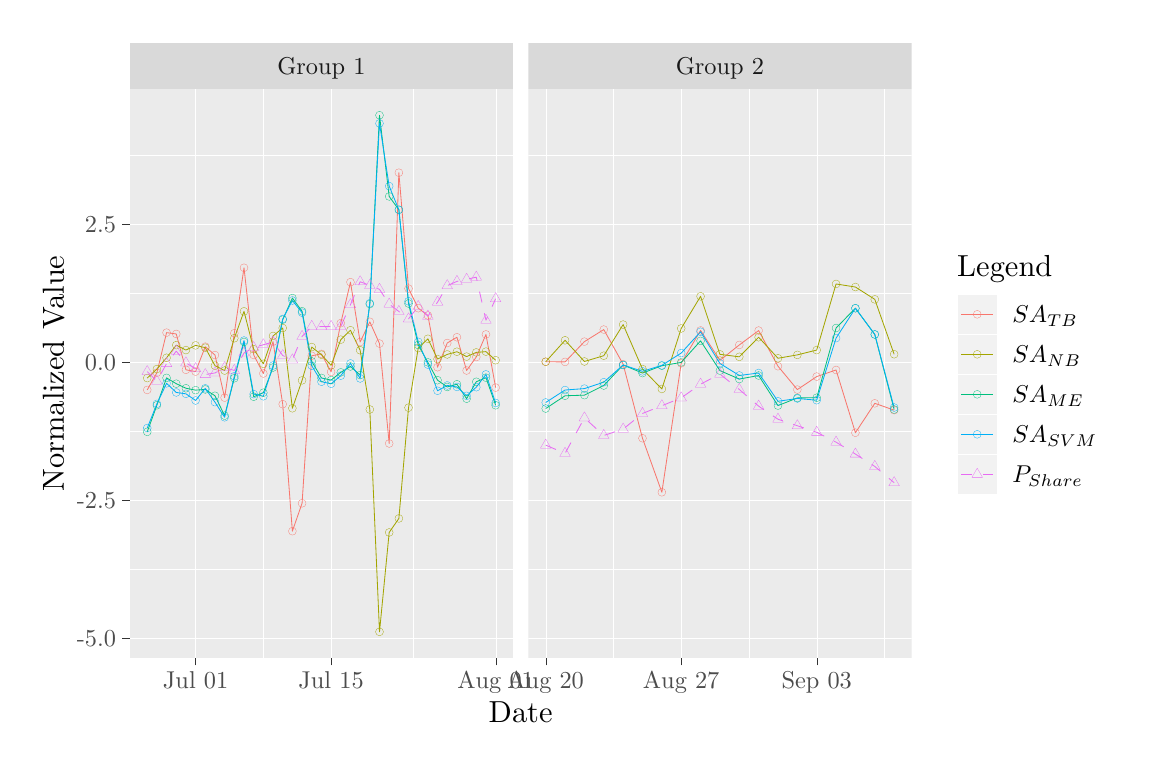
\begin{tikzpicture}[x=1pt,y=1pt]
\definecolor{fillColor}{RGB}{255,255,255}
\path[use as bounding box,fill=fillColor,fill opacity=0.00] (0,0) rectangle (397.48,258.37);
\begin{scope}
\path[clip] (  0.00,  0.00) rectangle (397.48,258.37);
\definecolor{drawColor}{RGB}{255,255,255}
\definecolor{fillColor}{RGB}{255,255,255}

\path[draw=drawColor,line width= 0.1pt,line join=round,line cap=round,fill=fillColor] (  0.00, -0.00) rectangle (397.48,258.37);
\end{scope}
\begin{scope}
\path[clip] ( 36.90, 30.73) rectangle (175.39,236.06);
\definecolor{fillColor}{gray}{0.92}

\path[fill=fillColor] ( 36.90, 30.73) rectangle (175.39,236.06);
\definecolor{drawColor}{RGB}{255,255,255}

\path[draw=drawColor,line width= 0.1pt,line join=round] ( 36.90, 62.84) --
	(175.39, 62.84);

\path[draw=drawColor,line width= 0.1pt,line join=round] ( 36.90,112.67) --
	(175.39,112.67);

\path[draw=drawColor,line width= 0.1pt,line join=round] ( 36.90,162.51) --
	(175.39,162.51);

\path[draw=drawColor,line width= 0.1pt,line join=round] ( 36.90,212.35) --
	(175.39,212.35);

\path[draw=drawColor,line width= 0.1pt,line join=round] ( 85.16, 30.73) --
	( 85.16,236.06);

\path[draw=drawColor,line width= 0.1pt,line join=round] (139.37, 30.73) --
	(139.37,236.06);

\path[draw=drawColor,line width= 0.1pt,line join=round] ( 36.90, 37.92) --
	(175.39, 37.92);

\path[draw=drawColor,line width= 0.1pt,line join=round] ( 36.90, 87.75) --
	(175.39, 87.75);

\path[draw=drawColor,line width= 0.1pt,line join=round] ( 36.90,137.59) --
	(175.39,137.59);

\path[draw=drawColor,line width= 0.1pt,line join=round] ( 36.90,187.43) --
	(175.39,187.43);

\path[draw=drawColor,line width= 0.1pt,line join=round] ( 60.68, 30.73) --
	( 60.68,236.06);

\path[draw=drawColor,line width= 0.1pt,line join=round] (109.64, 30.73) --
	(109.64,236.06);

\path[draw=drawColor,line width= 0.1pt,line join=round] (169.10, 30.73) --
	(169.10,236.06);
\definecolor{drawColor}{RGB}{248,118,109}

\path[draw=drawColor,line width= 0.3pt,line join=round] ( 43.20,127.47) --
	( 46.69,133.68) --
	( 50.19,148.17) --
	( 53.69,147.69) --
	( 57.18,134.74) --
	( 60.68,134.09) --
	( 64.18,143.10) --
	( 67.68,140.08) --
	( 71.17,124.68) --
	( 74.67,147.96) --
	( 78.17,171.61) --
	( 81.67,140.11) --
	( 85.16,133.40) --
	( 88.66,144.94) --
	( 92.16,122.32) --
	( 95.65, 76.43) --
	( 99.15, 86.51) --
	(102.65,139.81) --
	(106.15,140.49) --
	(109.64,133.99) --
	(113.14,151.60) --
	(116.64,166.41) --
	(120.14,144.78) --
	(123.63,152.08) --
	(127.13,144.22) --
	(130.63,108.12) --
	(134.13,205.96) --
	(137.62,164.09) --
	(141.12,157.01) --
	(144.62,154.37) --
	(148.11,135.67) --
	(151.61,144.42) --
	(155.11,146.51) --
	(158.61,134.49) --
	(162.10,139.36) --
	(165.60,147.53) --
	(169.10,128.31);
\definecolor{drawColor}{RGB}{163,165,0}

\path[draw=drawColor,line width= 0.3pt,line join=round] ( 43.20,131.75) --
	( 46.69,135.01) --
	( 50.19,139.09) --
	( 53.69,143.65) --
	( 57.18,141.87) --
	( 60.68,143.57) --
	( 64.18,142.73) --
	( 67.68,136.23) --
	( 71.17,134.47) --
	( 74.67,146.16) --
	( 78.17,155.87) --
	( 81.67,142.21) --
	( 85.16,136.91) --
	( 88.66,146.97) --
	( 92.16,149.85) --
	( 95.65,120.84) --
	( 99.15,130.92) --
	(102.65,142.96) --
	(106.15,140.19) --
	(109.64,136.35) --
	(113.14,145.63) --
	(116.64,149.05) --
	(120.14,141.82) --
	(123.63,120.40) --
	(127.13, 40.06) --
	(130.63, 75.97) --
	(134.13, 81.04) --
	(137.62,121.06) --
	(141.12,142.60) --
	(144.62,145.94) --
	(148.11,138.62) --
	(151.61,140.30) --
	(155.11,141.27) --
	(158.61,139.51) --
	(162.10,141.03) --
	(165.60,141.31) --
	(169.10,138.21);
\definecolor{drawColor}{RGB}{0,191,125}

\path[draw=drawColor,line width= 0.3pt,line join=round] ( 43.20,112.32) --
	( 46.69,121.94) --
	( 50.19,131.82) --
	( 53.69,129.72) --
	( 57.18,128.08) --
	( 60.68,127.39) --
	( 64.18,127.65) --
	( 67.68,125.35) --
	( 71.17,118.17) --
	( 74.67,131.71) --
	( 78.17,144.80) --
	( 81.67,125.01) --
	( 85.16,126.46) --
	( 88.66,135.57) --
	( 92.16,152.85) --
	( 95.65,160.66) --
	( 99.15,155.91) --
	(102.65,137.78) --
	(106.15,131.80) --
	(109.64,131.02) --
	(113.14,133.82) --
	(116.64,135.95) --
	(120.14,132.83) --
	(123.63,158.49) --
	(127.13,226.73) --
	(130.63,197.39) --
	(134.13,192.58) --
	(137.62,158.70) --
	(141.12,143.71) --
	(144.62,137.43) --
	(148.11,130.99) --
	(151.61,128.54) --
	(155.11,129.52) --
	(158.61,124.30) --
	(162.10,130.41) --
	(165.60,131.90) --
	(169.10,121.93);
\definecolor{drawColor}{RGB}{0,176,246}

\path[draw=drawColor,line width= 0.3pt,line join=round] ( 43.20,113.69) --
	( 46.69,122.42) --
	( 50.19,129.86) --
	( 53.69,126.56) --
	( 57.18,126.06) --
	( 60.68,123.66) --
	( 64.18,128.05) --
	( 67.68,123.05) --
	( 71.17,117.58) --
	( 74.67,132.41) --
	( 78.17,145.32) --
	( 81.67,125.96) --
	( 85.16,125.18) --
	( 88.66,136.27) --
	( 92.16,153.10) --
	( 95.65,159.79) --
	( 99.15,155.38) --
	(102.65,136.22) --
	(106.15,130.43) --
	(109.64,129.69) --
	(113.14,132.62) --
	(116.64,137.05) --
	(120.14,131.62) --
	(123.63,158.79) --
	(127.13,223.78) --
	(130.63,201.11) --
	(134.13,192.54) --
	(137.62,159.49) --
	(141.12,144.84) --
	(144.62,136.62) --
	(148.11,127.16) --
	(151.61,129.09) --
	(155.11,128.55) --
	(158.61,125.33) --
	(162.10,128.46) --
	(165.60,133.08) --
	(169.10,122.76);
\definecolor{drawColor}{RGB}{231,107,243}

\path[draw=drawColor,line width= 0.3pt,dash pattern=on 4pt off 4pt ,line join=round] ( 43.20,134.10) --
	( 46.69,130.62) --
	( 50.19,137.00) --
	( 53.69,141.47) --
	( 57.18,137.25) --
	( 60.68,135.14) --
	( 64.18,133.02) --
	( 67.68,133.60) --
	( 71.17,135.51) --
	( 74.67,134.51) --
	( 78.17,140.81) --
	( 81.67,142.79) --
	( 85.16,143.79) --
	( 88.66,144.78) --
	( 92.16,139.90) --
	( 95.65,138.32) --
	( 99.15,146.77) --
	(102.65,150.41) --
	(106.15,150.41) --
	(109.64,150.41) --
	(113.14,150.41) --
	(116.64,158.28) --
	(120.14,166.56) --
	(123.63,165.23) --
	(127.13,163.82) --
	(130.63,158.48) --
	(134.13,155.81) --
	(137.62,153.14) --
	(141.12,157.61) --
	(144.62,154.14) --
	(148.11,159.19) --
	(151.61,165.15) --
	(155.11,166.68) --
	(158.61,167.45) --
	(162.10,168.21) --
	(165.60,152.65) --
	(169.10,160.43);
\definecolor{drawColor}{RGB}{248,118,109}

\path[draw=drawColor,line width= 0.1pt,line join=round,line cap=round] ( 43.20,127.47) circle (  1.43);

\path[draw=drawColor,line width= 0.1pt,line join=round,line cap=round] ( 46.69,133.68) circle (  1.43);

\path[draw=drawColor,line width= 0.1pt,line join=round,line cap=round] ( 50.19,148.17) circle (  1.43);

\path[draw=drawColor,line width= 0.1pt,line join=round,line cap=round] ( 53.69,147.69) circle (  1.43);

\path[draw=drawColor,line width= 0.1pt,line join=round,line cap=round] ( 57.18,134.74) circle (  1.43);

\path[draw=drawColor,line width= 0.1pt,line join=round,line cap=round] ( 60.68,134.09) circle (  1.43);

\path[draw=drawColor,line width= 0.1pt,line join=round,line cap=round] ( 64.18,143.10) circle (  1.43);

\path[draw=drawColor,line width= 0.1pt,line join=round,line cap=round] ( 67.68,140.08) circle (  1.43);

\path[draw=drawColor,line width= 0.1pt,line join=round,line cap=round] ( 71.17,124.68) circle (  1.43);

\path[draw=drawColor,line width= 0.1pt,line join=round,line cap=round] ( 74.67,147.96) circle (  1.43);

\path[draw=drawColor,line width= 0.1pt,line join=round,line cap=round] ( 78.17,171.61) circle (  1.43);

\path[draw=drawColor,line width= 0.1pt,line join=round,line cap=round] ( 81.67,140.11) circle (  1.43);

\path[draw=drawColor,line width= 0.1pt,line join=round,line cap=round] ( 85.16,133.40) circle (  1.43);

\path[draw=drawColor,line width= 0.1pt,line join=round,line cap=round] ( 88.66,144.94) circle (  1.43);

\path[draw=drawColor,line width= 0.1pt,line join=round,line cap=round] ( 92.16,122.32) circle (  1.43);

\path[draw=drawColor,line width= 0.1pt,line join=round,line cap=round] ( 95.65, 76.43) circle (  1.43);

\path[draw=drawColor,line width= 0.1pt,line join=round,line cap=round] ( 99.15, 86.51) circle (  1.43);

\path[draw=drawColor,line width= 0.1pt,line join=round,line cap=round] (102.65,139.81) circle (  1.43);

\path[draw=drawColor,line width= 0.1pt,line join=round,line cap=round] (106.15,140.49) circle (  1.43);

\path[draw=drawColor,line width= 0.1pt,line join=round,line cap=round] (109.64,133.99) circle (  1.43);

\path[draw=drawColor,line width= 0.1pt,line join=round,line cap=round] (113.14,151.60) circle (  1.43);

\path[draw=drawColor,line width= 0.1pt,line join=round,line cap=round] (116.64,166.41) circle (  1.43);

\path[draw=drawColor,line width= 0.1pt,line join=round,line cap=round] (120.14,144.78) circle (  1.43);

\path[draw=drawColor,line width= 0.1pt,line join=round,line cap=round] (123.63,152.08) circle (  1.43);

\path[draw=drawColor,line width= 0.1pt,line join=round,line cap=round] (127.13,144.22) circle (  1.43);

\path[draw=drawColor,line width= 0.1pt,line join=round,line cap=round] (130.63,108.12) circle (  1.43);

\path[draw=drawColor,line width= 0.1pt,line join=round,line cap=round] (134.13,205.96) circle (  1.43);

\path[draw=drawColor,line width= 0.1pt,line join=round,line cap=round] (137.62,164.09) circle (  1.43);

\path[draw=drawColor,line width= 0.1pt,line join=round,line cap=round] (141.12,157.01) circle (  1.43);

\path[draw=drawColor,line width= 0.1pt,line join=round,line cap=round] (144.62,154.37) circle (  1.43);

\path[draw=drawColor,line width= 0.1pt,line join=round,line cap=round] (148.11,135.67) circle (  1.43);

\path[draw=drawColor,line width= 0.1pt,line join=round,line cap=round] (151.61,144.42) circle (  1.43);

\path[draw=drawColor,line width= 0.1pt,line join=round,line cap=round] (155.11,146.51) circle (  1.43);

\path[draw=drawColor,line width= 0.1pt,line join=round,line cap=round] (158.61,134.49) circle (  1.43);

\path[draw=drawColor,line width= 0.1pt,line join=round,line cap=round] (162.10,139.36) circle (  1.43);

\path[draw=drawColor,line width= 0.1pt,line join=round,line cap=round] (165.60,147.53) circle (  1.43);

\path[draw=drawColor,line width= 0.1pt,line join=round,line cap=round] (169.10,128.31) circle (  1.43);
\definecolor{drawColor}{RGB}{163,165,0}

\path[draw=drawColor,line width= 0.1pt,line join=round,line cap=round] ( 43.20,131.75) circle (  1.43);

\path[draw=drawColor,line width= 0.1pt,line join=round,line cap=round] ( 46.69,135.01) circle (  1.43);

\path[draw=drawColor,line width= 0.1pt,line join=round,line cap=round] ( 50.19,139.09) circle (  1.43);

\path[draw=drawColor,line width= 0.1pt,line join=round,line cap=round] ( 53.69,143.65) circle (  1.43);

\path[draw=drawColor,line width= 0.1pt,line join=round,line cap=round] ( 57.18,141.87) circle (  1.43);

\path[draw=drawColor,line width= 0.1pt,line join=round,line cap=round] ( 60.68,143.57) circle (  1.43);

\path[draw=drawColor,line width= 0.1pt,line join=round,line cap=round] ( 64.18,142.73) circle (  1.43);

\path[draw=drawColor,line width= 0.1pt,line join=round,line cap=round] ( 67.68,136.23) circle (  1.43);

\path[draw=drawColor,line width= 0.1pt,line join=round,line cap=round] ( 71.17,134.47) circle (  1.43);

\path[draw=drawColor,line width= 0.1pt,line join=round,line cap=round] ( 74.67,146.16) circle (  1.43);

\path[draw=drawColor,line width= 0.1pt,line join=round,line cap=round] ( 78.17,155.87) circle (  1.43);

\path[draw=drawColor,line width= 0.1pt,line join=round,line cap=round] ( 81.67,142.21) circle (  1.43);

\path[draw=drawColor,line width= 0.1pt,line join=round,line cap=round] ( 85.16,136.91) circle (  1.43);

\path[draw=drawColor,line width= 0.1pt,line join=round,line cap=round] ( 88.66,146.97) circle (  1.43);

\path[draw=drawColor,line width= 0.1pt,line join=round,line cap=round] ( 92.16,149.85) circle (  1.43);

\path[draw=drawColor,line width= 0.1pt,line join=round,line cap=round] ( 95.65,120.84) circle (  1.43);

\path[draw=drawColor,line width= 0.1pt,line join=round,line cap=round] ( 99.15,130.92) circle (  1.43);

\path[draw=drawColor,line width= 0.1pt,line join=round,line cap=round] (102.65,142.96) circle (  1.43);

\path[draw=drawColor,line width= 0.1pt,line join=round,line cap=round] (106.15,140.19) circle (  1.43);

\path[draw=drawColor,line width= 0.1pt,line join=round,line cap=round] (109.64,136.35) circle (  1.43);

\path[draw=drawColor,line width= 0.1pt,line join=round,line cap=round] (113.14,145.63) circle (  1.43);

\path[draw=drawColor,line width= 0.1pt,line join=round,line cap=round] (116.64,149.05) circle (  1.43);

\path[draw=drawColor,line width= 0.1pt,line join=round,line cap=round] (120.14,141.82) circle (  1.43);

\path[draw=drawColor,line width= 0.1pt,line join=round,line cap=round] (123.63,120.40) circle (  1.43);

\path[draw=drawColor,line width= 0.1pt,line join=round,line cap=round] (127.13, 40.06) circle (  1.43);

\path[draw=drawColor,line width= 0.1pt,line join=round,line cap=round] (130.63, 75.97) circle (  1.43);

\path[draw=drawColor,line width= 0.1pt,line join=round,line cap=round] (134.13, 81.04) circle (  1.43);

\path[draw=drawColor,line width= 0.1pt,line join=round,line cap=round] (137.62,121.06) circle (  1.43);

\path[draw=drawColor,line width= 0.1pt,line join=round,line cap=round] (141.12,142.60) circle (  1.43);

\path[draw=drawColor,line width= 0.1pt,line join=round,line cap=round] (144.62,145.94) circle (  1.43);

\path[draw=drawColor,line width= 0.1pt,line join=round,line cap=round] (148.11,138.62) circle (  1.43);

\path[draw=drawColor,line width= 0.1pt,line join=round,line cap=round] (151.61,140.30) circle (  1.43);

\path[draw=drawColor,line width= 0.1pt,line join=round,line cap=round] (155.11,141.27) circle (  1.43);

\path[draw=drawColor,line width= 0.1pt,line join=round,line cap=round] (158.61,139.51) circle (  1.43);

\path[draw=drawColor,line width= 0.1pt,line join=round,line cap=round] (162.10,141.03) circle (  1.43);

\path[draw=drawColor,line width= 0.1pt,line join=round,line cap=round] (165.60,141.31) circle (  1.43);

\path[draw=drawColor,line width= 0.1pt,line join=round,line cap=round] (169.10,138.21) circle (  1.43);
\definecolor{drawColor}{RGB}{0,191,125}

\path[draw=drawColor,line width= 0.1pt,line join=round,line cap=round] ( 43.20,112.32) circle (  1.43);

\path[draw=drawColor,line width= 0.1pt,line join=round,line cap=round] ( 46.69,121.94) circle (  1.43);

\path[draw=drawColor,line width= 0.1pt,line join=round,line cap=round] ( 50.19,131.82) circle (  1.43);

\path[draw=drawColor,line width= 0.1pt,line join=round,line cap=round] ( 53.69,129.72) circle (  1.43);

\path[draw=drawColor,line width= 0.1pt,line join=round,line cap=round] ( 57.18,128.08) circle (  1.43);

\path[draw=drawColor,line width= 0.1pt,line join=round,line cap=round] ( 60.68,127.39) circle (  1.43);

\path[draw=drawColor,line width= 0.1pt,line join=round,line cap=round] ( 64.18,127.65) circle (  1.43);

\path[draw=drawColor,line width= 0.1pt,line join=round,line cap=round] ( 67.68,125.35) circle (  1.43);

\path[draw=drawColor,line width= 0.1pt,line join=round,line cap=round] ( 71.17,118.17) circle (  1.43);

\path[draw=drawColor,line width= 0.1pt,line join=round,line cap=round] ( 74.67,131.71) circle (  1.43);

\path[draw=drawColor,line width= 0.1pt,line join=round,line cap=round] ( 78.17,144.80) circle (  1.43);

\path[draw=drawColor,line width= 0.1pt,line join=round,line cap=round] ( 81.67,125.01) circle (  1.43);

\path[draw=drawColor,line width= 0.1pt,line join=round,line cap=round] ( 85.16,126.46) circle (  1.43);

\path[draw=drawColor,line width= 0.1pt,line join=round,line cap=round] ( 88.66,135.57) circle (  1.43);

\path[draw=drawColor,line width= 0.1pt,line join=round,line cap=round] ( 92.16,152.85) circle (  1.43);

\path[draw=drawColor,line width= 0.1pt,line join=round,line cap=round] ( 95.65,160.66) circle (  1.43);

\path[draw=drawColor,line width= 0.1pt,line join=round,line cap=round] ( 99.15,155.91) circle (  1.43);

\path[draw=drawColor,line width= 0.1pt,line join=round,line cap=round] (102.65,137.78) circle (  1.43);

\path[draw=drawColor,line width= 0.1pt,line join=round,line cap=round] (106.15,131.80) circle (  1.43);

\path[draw=drawColor,line width= 0.1pt,line join=round,line cap=round] (109.64,131.02) circle (  1.43);

\path[draw=drawColor,line width= 0.1pt,line join=round,line cap=round] (113.14,133.82) circle (  1.43);

\path[draw=drawColor,line width= 0.1pt,line join=round,line cap=round] (116.64,135.95) circle (  1.43);

\path[draw=drawColor,line width= 0.1pt,line join=round,line cap=round] (120.14,132.83) circle (  1.43);

\path[draw=drawColor,line width= 0.1pt,line join=round,line cap=round] (123.63,158.49) circle (  1.43);

\path[draw=drawColor,line width= 0.1pt,line join=round,line cap=round] (127.13,226.73) circle (  1.43);

\path[draw=drawColor,line width= 0.1pt,line join=round,line cap=round] (130.63,197.39) circle (  1.43);

\path[draw=drawColor,line width= 0.1pt,line join=round,line cap=round] (134.13,192.58) circle (  1.43);

\path[draw=drawColor,line width= 0.1pt,line join=round,line cap=round] (137.62,158.70) circle (  1.43);

\path[draw=drawColor,line width= 0.1pt,line join=round,line cap=round] (141.12,143.71) circle (  1.43);

\path[draw=drawColor,line width= 0.1pt,line join=round,line cap=round] (144.62,137.43) circle (  1.43);

\path[draw=drawColor,line width= 0.1pt,line join=round,line cap=round] (148.11,130.99) circle (  1.43);

\path[draw=drawColor,line width= 0.1pt,line join=round,line cap=round] (151.61,128.54) circle (  1.43);

\path[draw=drawColor,line width= 0.1pt,line join=round,line cap=round] (155.11,129.52) circle (  1.43);

\path[draw=drawColor,line width= 0.1pt,line join=round,line cap=round] (158.61,124.30) circle (  1.43);

\path[draw=drawColor,line width= 0.1pt,line join=round,line cap=round] (162.10,130.41) circle (  1.43);

\path[draw=drawColor,line width= 0.1pt,line join=round,line cap=round] (165.60,131.90) circle (  1.43);

\path[draw=drawColor,line width= 0.1pt,line join=round,line cap=round] (169.10,121.93) circle (  1.43);
\definecolor{drawColor}{RGB}{0,176,246}

\path[draw=drawColor,line width= 0.1pt,line join=round,line cap=round] ( 43.20,113.69) circle (  1.43);

\path[draw=drawColor,line width= 0.1pt,line join=round,line cap=round] ( 46.69,122.42) circle (  1.43);

\path[draw=drawColor,line width= 0.1pt,line join=round,line cap=round] ( 50.19,129.86) circle (  1.43);

\path[draw=drawColor,line width= 0.1pt,line join=round,line cap=round] ( 53.69,126.56) circle (  1.43);

\path[draw=drawColor,line width= 0.1pt,line join=round,line cap=round] ( 57.18,126.06) circle (  1.43);

\path[draw=drawColor,line width= 0.1pt,line join=round,line cap=round] ( 60.68,123.66) circle (  1.43);

\path[draw=drawColor,line width= 0.1pt,line join=round,line cap=round] ( 64.18,128.05) circle (  1.43);

\path[draw=drawColor,line width= 0.1pt,line join=round,line cap=round] ( 67.68,123.05) circle (  1.43);

\path[draw=drawColor,line width= 0.1pt,line join=round,line cap=round] ( 71.17,117.58) circle (  1.43);

\path[draw=drawColor,line width= 0.1pt,line join=round,line cap=round] ( 74.67,132.41) circle (  1.43);

\path[draw=drawColor,line width= 0.1pt,line join=round,line cap=round] ( 78.17,145.32) circle (  1.43);

\path[draw=drawColor,line width= 0.1pt,line join=round,line cap=round] ( 81.67,125.96) circle (  1.43);

\path[draw=drawColor,line width= 0.1pt,line join=round,line cap=round] ( 85.16,125.18) circle (  1.43);

\path[draw=drawColor,line width= 0.1pt,line join=round,line cap=round] ( 88.66,136.27) circle (  1.43);

\path[draw=drawColor,line width= 0.1pt,line join=round,line cap=round] ( 92.16,153.10) circle (  1.43);

\path[draw=drawColor,line width= 0.1pt,line join=round,line cap=round] ( 95.65,159.79) circle (  1.43);

\path[draw=drawColor,line width= 0.1pt,line join=round,line cap=round] ( 99.15,155.38) circle (  1.43);

\path[draw=drawColor,line width= 0.1pt,line join=round,line cap=round] (102.65,136.22) circle (  1.43);

\path[draw=drawColor,line width= 0.1pt,line join=round,line cap=round] (106.15,130.43) circle (  1.43);

\path[draw=drawColor,line width= 0.1pt,line join=round,line cap=round] (109.64,129.69) circle (  1.43);

\path[draw=drawColor,line width= 0.1pt,line join=round,line cap=round] (113.14,132.62) circle (  1.43);

\path[draw=drawColor,line width= 0.1pt,line join=round,line cap=round] (116.64,137.05) circle (  1.43);

\path[draw=drawColor,line width= 0.1pt,line join=round,line cap=round] (120.14,131.62) circle (  1.43);

\path[draw=drawColor,line width= 0.1pt,line join=round,line cap=round] (123.63,158.79) circle (  1.43);

\path[draw=drawColor,line width= 0.1pt,line join=round,line cap=round] (127.13,223.78) circle (  1.43);

\path[draw=drawColor,line width= 0.1pt,line join=round,line cap=round] (130.63,201.11) circle (  1.43);

\path[draw=drawColor,line width= 0.1pt,line join=round,line cap=round] (134.13,192.54) circle (  1.43);

\path[draw=drawColor,line width= 0.1pt,line join=round,line cap=round] (137.62,159.49) circle (  1.43);

\path[draw=drawColor,line width= 0.1pt,line join=round,line cap=round] (141.12,144.84) circle (  1.43);

\path[draw=drawColor,line width= 0.1pt,line join=round,line cap=round] (144.62,136.62) circle (  1.43);

\path[draw=drawColor,line width= 0.1pt,line join=round,line cap=round] (148.11,127.16) circle (  1.43);

\path[draw=drawColor,line width= 0.1pt,line join=round,line cap=round] (151.61,129.09) circle (  1.43);

\path[draw=drawColor,line width= 0.1pt,line join=round,line cap=round] (155.11,128.55) circle (  1.43);

\path[draw=drawColor,line width= 0.1pt,line join=round,line cap=round] (158.61,125.33) circle (  1.43);

\path[draw=drawColor,line width= 0.1pt,line join=round,line cap=round] (162.10,128.46) circle (  1.43);

\path[draw=drawColor,line width= 0.1pt,line join=round,line cap=round] (165.60,133.08) circle (  1.43);

\path[draw=drawColor,line width= 0.1pt,line join=round,line cap=round] (169.10,122.76) circle (  1.43);
\definecolor{drawColor}{RGB}{231,107,243}

\path[draw=drawColor,line width= 0.1pt,line join=round,line cap=round] ( 43.20,136.32) --
	( 45.12,132.99) --
	( 41.27,132.99) --
	( 43.20,136.32);

\path[draw=drawColor,line width= 0.1pt,line join=round,line cap=round] ( 46.69,132.84) --
	( 48.61,129.51) --
	( 44.77,129.51) --
	( 46.69,132.84);

\path[draw=drawColor,line width= 0.1pt,line join=round,line cap=round] ( 50.19,139.22) --
	( 52.11,135.89) --
	( 48.27,135.89) --
	( 50.19,139.22);

\path[draw=drawColor,line width= 0.1pt,line join=round,line cap=round] ( 53.69,143.69) --
	( 55.61,140.36) --
	( 51.77,140.36) --
	( 53.69,143.69);

\path[draw=drawColor,line width= 0.1pt,line join=round,line cap=round] ( 57.18,139.47) --
	( 59.11,136.14) --
	( 55.26,136.14) --
	( 57.18,139.47);

\path[draw=drawColor,line width= 0.1pt,line join=round,line cap=round] ( 60.68,137.35) --
	( 62.60,134.03) --
	( 58.76,134.03) --
	( 60.68,137.35);

\path[draw=drawColor,line width= 0.1pt,line join=round,line cap=round] ( 64.18,135.24) --
	( 66.10,131.91) --
	( 62.26,131.91) --
	( 64.18,135.24);

\path[draw=drawColor,line width= 0.1pt,line join=round,line cap=round] ( 67.68,135.82) --
	( 69.60,132.49) --
	( 65.75,132.49) --
	( 67.68,135.82);

\path[draw=drawColor,line width= 0.1pt,line join=round,line cap=round] ( 71.17,137.73) --
	( 73.09,134.40) --
	( 69.25,134.40) --
	( 71.17,137.73);

\path[draw=drawColor,line width= 0.1pt,line join=round,line cap=round] ( 74.67,136.73) --
	( 76.59,133.41) --
	( 72.75,133.41) --
	( 74.67,136.73);

\path[draw=drawColor,line width= 0.1pt,line join=round,line cap=round] ( 78.17,143.03) --
	( 80.09,139.70) --
	( 76.25,139.70) --
	( 78.17,143.03);

\path[draw=drawColor,line width= 0.1pt,line join=round,line cap=round] ( 81.67,145.01) --
	( 83.59,141.68) --
	( 79.74,141.68) --
	( 81.67,145.01);

\path[draw=drawColor,line width= 0.1pt,line join=round,line cap=round] ( 85.16,146.01) --
	( 87.08,142.68) --
	( 83.24,142.68) --
	( 85.16,146.01);

\path[draw=drawColor,line width= 0.1pt,line join=round,line cap=round] ( 88.66,147.00) --
	( 90.58,143.67) --
	( 86.74,143.67) --
	( 88.66,147.00);

\path[draw=drawColor,line width= 0.1pt,line join=round,line cap=round] ( 92.16,142.11) --
	( 94.08,138.79) --
	( 90.24,138.79) --
	( 92.16,142.11);

\path[draw=drawColor,line width= 0.1pt,line join=round,line cap=round] ( 95.65,140.54) --
	( 97.58,137.21) --
	( 93.73,137.21) --
	( 95.65,140.54);

\path[draw=drawColor,line width= 0.1pt,line join=round,line cap=round] ( 99.15,148.99) --
	(101.07,145.66) --
	( 97.23,145.66) --
	( 99.15,148.99);

\path[draw=drawColor,line width= 0.1pt,line join=round,line cap=round] (102.65,152.63) --
	(104.57,149.30) --
	(100.73,149.30) --
	(102.65,152.63);

\path[draw=drawColor,line width= 0.1pt,line join=round,line cap=round] (106.15,152.63) --
	(108.07,149.30) --
	(104.23,149.30) --
	(106.15,152.63);

\path[draw=drawColor,line width= 0.1pt,line join=round,line cap=round] (109.64,152.63) --
	(111.57,149.30) --
	(107.72,149.30) --
	(109.64,152.63);

\path[draw=drawColor,line width= 0.1pt,line join=round,line cap=round] (113.14,152.63) --
	(115.06,149.30) --
	(111.22,149.30) --
	(113.14,152.63);

\path[draw=drawColor,line width= 0.1pt,line join=round,line cap=round] (116.64,160.49) --
	(118.56,157.17) --
	(114.72,157.17) --
	(116.64,160.49);

\path[draw=drawColor,line width= 0.1pt,line join=round,line cap=round] (120.14,168.77) --
	(122.06,165.45) --
	(118.21,165.45) --
	(120.14,168.77);

\path[draw=drawColor,line width= 0.1pt,line join=round,line cap=round] (123.63,167.45) --
	(125.55,164.12) --
	(121.71,164.12) --
	(123.63,167.45);

\path[draw=drawColor,line width= 0.1pt,line join=round,line cap=round] (127.13,166.04) --
	(129.05,162.71) --
	(125.21,162.71) --
	(127.13,166.04);

\path[draw=drawColor,line width= 0.1pt,line join=round,line cap=round] (130.63,160.70) --
	(132.55,157.37) --
	(128.71,157.37) --
	(130.63,160.70);

\path[draw=drawColor,line width= 0.1pt,line join=round,line cap=round] (134.13,158.03) --
	(136.05,154.70) --
	(132.20,154.70) --
	(134.13,158.03);

\path[draw=drawColor,line width= 0.1pt,line join=round,line cap=round] (137.62,155.36) --
	(139.54,152.03) --
	(135.70,152.03) --
	(137.62,155.36);

\path[draw=drawColor,line width= 0.1pt,line join=round,line cap=round] (141.12,159.83) --
	(143.04,156.50) --
	(139.20,156.50) --
	(141.12,159.83);

\path[draw=drawColor,line width= 0.1pt,line join=round,line cap=round] (144.62,156.36) --
	(146.54,153.03) --
	(142.70,153.03) --
	(144.62,156.36);

\path[draw=drawColor,line width= 0.1pt,line join=round,line cap=round] (148.11,161.41) --
	(150.04,158.08) --
	(146.19,158.08) --
	(148.11,161.41);

\path[draw=drawColor,line width= 0.1pt,line join=round,line cap=round] (151.61,167.37) --
	(153.53,164.04) --
	(149.69,164.04) --
	(151.61,167.37);

\path[draw=drawColor,line width= 0.1pt,line join=round,line cap=round] (155.11,168.90) --
	(157.03,165.57) --
	(153.19,165.57) --
	(155.11,168.90);

\path[draw=drawColor,line width= 0.1pt,line join=round,line cap=round] (158.61,169.66) --
	(160.53,166.34) --
	(156.69,166.34) --
	(158.61,169.66);

\path[draw=drawColor,line width= 0.1pt,line join=round,line cap=round] (162.10,170.43) --
	(164.03,167.10) --
	(160.18,167.10) --
	(162.10,170.43);

\path[draw=drawColor,line width= 0.1pt,line join=round,line cap=round] (165.60,154.86) --
	(167.52,151.54) --
	(163.68,151.54) --
	(165.60,154.86);

\path[draw=drawColor,line width= 0.1pt,line join=round,line cap=round] (169.10,162.65) --
	(171.02,159.32) --
	(167.18,159.32) --
	(169.10,162.65);
\end{scope}
\begin{scope}
\path[clip] (180.89, 30.73) rectangle (319.39,236.06);
\definecolor{fillColor}{gray}{0.92}

\path[fill=fillColor] (180.89, 30.73) rectangle (319.39,236.06);
\definecolor{drawColor}{RGB}{255,255,255}

\path[draw=drawColor,line width= 0.1pt,line join=round] (180.89, 62.84) --
	(319.39, 62.84);

\path[draw=drawColor,line width= 0.1pt,line join=round] (180.89,112.67) --
	(319.39,112.67);

\path[draw=drawColor,line width= 0.1pt,line join=round] (180.89,162.51) --
	(319.39,162.51);

\path[draw=drawColor,line width= 0.1pt,line join=round] (180.89,212.35) --
	(319.39,212.35);

\path[draw=drawColor,line width= 0.1pt,line join=round] (211.67, 30.73) --
	(211.67,236.06);

\path[draw=drawColor,line width= 0.1pt,line join=round] (260.63, 30.73) --
	(260.63,236.06);

\path[draw=drawColor,line width= 0.1pt,line join=round] (309.59, 30.73) --
	(309.59,236.06);

\path[draw=drawColor,line width= 0.1pt,line join=round] (180.89, 37.92) --
	(319.39, 37.92);

\path[draw=drawColor,line width= 0.1pt,line join=round] (180.89, 87.75) --
	(319.39, 87.75);

\path[draw=drawColor,line width= 0.1pt,line join=round] (180.89,137.59) --
	(319.39,137.59);

\path[draw=drawColor,line width= 0.1pt,line join=round] (180.89,187.43) --
	(319.39,187.43);

\path[draw=drawColor,line width= 0.1pt,line join=round] (187.19, 30.73) --
	(187.19,236.06);

\path[draw=drawColor,line width= 0.1pt,line join=round] (236.15, 30.73) --
	(236.15,236.06);

\path[draw=drawColor,line width= 0.1pt,line join=round] (285.11, 30.73) --
	(285.11,236.06);
\definecolor{drawColor}{RGB}{248,118,109}

\path[draw=drawColor,line width= 0.3pt,line join=round] (187.19,137.65) --
	(194.18,137.59) --
	(201.18,144.92) --
	(208.17,149.28) --
	(215.17,136.76) --
	(222.16,110.01) --
	(229.16, 90.49) --
	(236.15,137.09) --
	(243.15,148.97) --
	(250.14,138.15) --
	(257.14,143.72) --
	(264.13,148.92) --
	(271.12,136.04) --
	(278.12,127.59) --
	(285.11,132.29) --
	(292.11,134.68) --
	(299.10,112.01) --
	(306.10,122.63) --
	(313.09,120.16);
\definecolor{drawColor}{RGB}{163,165,0}

\path[draw=drawColor,line width= 0.3pt,line join=round] (187.19,137.65) --
	(194.18,145.41) --
	(201.18,137.75) --
	(208.17,139.84) --
	(215.17,151.08) --
	(222.16,135.02) --
	(229.16,127.82) --
	(236.15,149.69) --
	(243.15,161.29) --
	(250.14,140.33) --
	(257.14,139.43) --
	(264.13,146.51) --
	(271.12,138.91) --
	(278.12,140.13) --
	(285.11,141.87) --
	(292.11,165.76) --
	(299.10,164.65) --
	(306.10,160.20) --
	(313.09,140.37);
\definecolor{drawColor}{RGB}{0,191,125}

\path[draw=drawColor,line width= 0.3pt,line join=round] (187.19,120.75) --
	(194.18,125.36) --
	(201.18,125.58) --
	(208.17,129.06) --
	(215.17,136.48) --
	(222.16,133.56) --
	(229.16,136.21) --
	(236.15,137.41) --
	(243.15,145.20) --
	(250.14,134.44) --
	(257.14,131.41) --
	(264.13,132.67) --
	(271.12,121.81) --
	(278.12,124.58) --
	(285.11,124.65) --
	(292.11,149.84) --
	(299.10,157.00) --
	(306.10,147.50) --
	(313.09,120.39);
\definecolor{drawColor}{RGB}{0,176,246}

\path[draw=drawColor,line width= 0.3pt,line join=round] (187.19,122.93) --
	(194.18,127.43) --
	(201.18,127.95) --
	(208.17,130.26) --
	(215.17,136.49) --
	(222.16,134.19) --
	(229.16,136.35) --
	(236.15,140.79) --
	(243.15,148.49) --
	(250.14,137.03) --
	(257.14,132.69) --
	(264.13,133.58) --
	(271.12,123.36) --
	(278.12,124.38) --
	(285.11,123.76) --
	(292.11,146.20) --
	(299.10,156.98) --
	(306.10,147.54) --
	(313.09,121.10);
\definecolor{drawColor}{RGB}{231,107,243}

\path[draw=drawColor,line width= 0.3pt,dash pattern=on 4pt off 4pt ,line join=round] (187.19,107.52) --
	(194.18,104.54) --
	(201.18,117.38) --
	(208.17,111.00) --
	(215.17,113.32) --
	(222.16,118.95) --
	(229.16,121.76) --
	(236.15,124.58) --
	(243.15,129.55) --
	(250.14,133.19) --
	(257.14,127.64) --
	(264.13,121.60) --
	(271.12,116.88) --
	(278.12,114.52) --
	(285.11,112.16) --
	(292.11,108.60) --
	(299.10,104.29) --
	(306.10, 99.82) --
	(313.09, 93.95);
\definecolor{drawColor}{RGB}{248,118,109}

\path[draw=drawColor,line width= 0.1pt,line join=round,line cap=round] (187.19,137.65) circle (  1.43);

\path[draw=drawColor,line width= 0.1pt,line join=round,line cap=round] (194.18,137.59) circle (  1.43);

\path[draw=drawColor,line width= 0.1pt,line join=round,line cap=round] (201.18,144.92) circle (  1.43);

\path[draw=drawColor,line width= 0.1pt,line join=round,line cap=round] (208.17,149.28) circle (  1.43);

\path[draw=drawColor,line width= 0.1pt,line join=round,line cap=round] (215.17,136.76) circle (  1.43);

\path[draw=drawColor,line width= 0.1pt,line join=round,line cap=round] (222.16,110.01) circle (  1.43);

\path[draw=drawColor,line width= 0.1pt,line join=round,line cap=round] (229.16, 90.49) circle (  1.43);

\path[draw=drawColor,line width= 0.1pt,line join=round,line cap=round] (236.15,137.09) circle (  1.43);

\path[draw=drawColor,line width= 0.1pt,line join=round,line cap=round] (243.15,148.97) circle (  1.43);

\path[draw=drawColor,line width= 0.1pt,line join=round,line cap=round] (250.14,138.15) circle (  1.43);

\path[draw=drawColor,line width= 0.1pt,line join=round,line cap=round] (257.14,143.72) circle (  1.43);

\path[draw=drawColor,line width= 0.1pt,line join=round,line cap=round] (264.13,148.92) circle (  1.43);

\path[draw=drawColor,line width= 0.1pt,line join=round,line cap=round] (271.12,136.04) circle (  1.43);

\path[draw=drawColor,line width= 0.1pt,line join=round,line cap=round] (278.12,127.59) circle (  1.43);

\path[draw=drawColor,line width= 0.1pt,line join=round,line cap=round] (285.11,132.29) circle (  1.43);

\path[draw=drawColor,line width= 0.1pt,line join=round,line cap=round] (292.11,134.68) circle (  1.43);

\path[draw=drawColor,line width= 0.1pt,line join=round,line cap=round] (299.10,112.01) circle (  1.43);

\path[draw=drawColor,line width= 0.1pt,line join=round,line cap=round] (306.10,122.63) circle (  1.43);

\path[draw=drawColor,line width= 0.1pt,line join=round,line cap=round] (313.09,120.16) circle (  1.43);
\definecolor{drawColor}{RGB}{163,165,0}

\path[draw=drawColor,line width= 0.1pt,line join=round,line cap=round] (187.19,137.65) circle (  1.43);

\path[draw=drawColor,line width= 0.1pt,line join=round,line cap=round] (194.18,145.41) circle (  1.43);

\path[draw=drawColor,line width= 0.1pt,line join=round,line cap=round] (201.18,137.75) circle (  1.43);

\path[draw=drawColor,line width= 0.1pt,line join=round,line cap=round] (208.17,139.84) circle (  1.43);

\path[draw=drawColor,line width= 0.1pt,line join=round,line cap=round] (215.17,151.08) circle (  1.43);

\path[draw=drawColor,line width= 0.1pt,line join=round,line cap=round] (222.16,135.02) circle (  1.43);

\path[draw=drawColor,line width= 0.1pt,line join=round,line cap=round] (229.16,127.82) circle (  1.43);

\path[draw=drawColor,line width= 0.1pt,line join=round,line cap=round] (236.15,149.69) circle (  1.43);

\path[draw=drawColor,line width= 0.1pt,line join=round,line cap=round] (243.15,161.29) circle (  1.43);

\path[draw=drawColor,line width= 0.1pt,line join=round,line cap=round] (250.14,140.33) circle (  1.43);

\path[draw=drawColor,line width= 0.1pt,line join=round,line cap=round] (257.14,139.43) circle (  1.43);

\path[draw=drawColor,line width= 0.1pt,line join=round,line cap=round] (264.13,146.51) circle (  1.43);

\path[draw=drawColor,line width= 0.1pt,line join=round,line cap=round] (271.12,138.91) circle (  1.43);

\path[draw=drawColor,line width= 0.1pt,line join=round,line cap=round] (278.12,140.13) circle (  1.43);

\path[draw=drawColor,line width= 0.1pt,line join=round,line cap=round] (285.11,141.87) circle (  1.43);

\path[draw=drawColor,line width= 0.1pt,line join=round,line cap=round] (292.11,165.76) circle (  1.43);

\path[draw=drawColor,line width= 0.1pt,line join=round,line cap=round] (299.10,164.65) circle (  1.43);

\path[draw=drawColor,line width= 0.1pt,line join=round,line cap=round] (306.10,160.20) circle (  1.43);

\path[draw=drawColor,line width= 0.1pt,line join=round,line cap=round] (313.09,140.37) circle (  1.43);
\definecolor{drawColor}{RGB}{0,191,125}

\path[draw=drawColor,line width= 0.1pt,line join=round,line cap=round] (187.19,120.75) circle (  1.43);

\path[draw=drawColor,line width= 0.1pt,line join=round,line cap=round] (194.18,125.36) circle (  1.43);

\path[draw=drawColor,line width= 0.1pt,line join=round,line cap=round] (201.18,125.58) circle (  1.43);

\path[draw=drawColor,line width= 0.1pt,line join=round,line cap=round] (208.17,129.06) circle (  1.43);

\path[draw=drawColor,line width= 0.1pt,line join=round,line cap=round] (215.17,136.48) circle (  1.43);

\path[draw=drawColor,line width= 0.1pt,line join=round,line cap=round] (222.16,133.56) circle (  1.43);

\path[draw=drawColor,line width= 0.1pt,line join=round,line cap=round] (229.16,136.21) circle (  1.43);

\path[draw=drawColor,line width= 0.1pt,line join=round,line cap=round] (236.15,137.41) circle (  1.43);

\path[draw=drawColor,line width= 0.1pt,line join=round,line cap=round] (243.15,145.20) circle (  1.43);

\path[draw=drawColor,line width= 0.1pt,line join=round,line cap=round] (250.14,134.44) circle (  1.43);

\path[draw=drawColor,line width= 0.1pt,line join=round,line cap=round] (257.14,131.41) circle (  1.43);

\path[draw=drawColor,line width= 0.1pt,line join=round,line cap=round] (264.13,132.67) circle (  1.43);

\path[draw=drawColor,line width= 0.1pt,line join=round,line cap=round] (271.12,121.81) circle (  1.43);

\path[draw=drawColor,line width= 0.1pt,line join=round,line cap=round] (278.12,124.58) circle (  1.43);

\path[draw=drawColor,line width= 0.1pt,line join=round,line cap=round] (285.11,124.65) circle (  1.43);

\path[draw=drawColor,line width= 0.1pt,line join=round,line cap=round] (292.11,149.84) circle (  1.43);

\path[draw=drawColor,line width= 0.1pt,line join=round,line cap=round] (299.10,157.00) circle (  1.43);

\path[draw=drawColor,line width= 0.1pt,line join=round,line cap=round] (306.10,147.50) circle (  1.43);

\path[draw=drawColor,line width= 0.1pt,line join=round,line cap=round] (313.09,120.39) circle (  1.43);
\definecolor{drawColor}{RGB}{0,176,246}

\path[draw=drawColor,line width= 0.1pt,line join=round,line cap=round] (187.19,122.93) circle (  1.43);

\path[draw=drawColor,line width= 0.1pt,line join=round,line cap=round] (194.18,127.43) circle (  1.43);

\path[draw=drawColor,line width= 0.1pt,line join=round,line cap=round] (201.18,127.95) circle (  1.43);

\path[draw=drawColor,line width= 0.1pt,line join=round,line cap=round] (208.17,130.26) circle (  1.43);

\path[draw=drawColor,line width= 0.1pt,line join=round,line cap=round] (215.17,136.49) circle (  1.43);

\path[draw=drawColor,line width= 0.1pt,line join=round,line cap=round] (222.16,134.19) circle (  1.43);

\path[draw=drawColor,line width= 0.1pt,line join=round,line cap=round] (229.16,136.35) circle (  1.43);

\path[draw=drawColor,line width= 0.1pt,line join=round,line cap=round] (236.15,140.79) circle (  1.43);

\path[draw=drawColor,line width= 0.1pt,line join=round,line cap=round] (243.15,148.49) circle (  1.43);

\path[draw=drawColor,line width= 0.1pt,line join=round,line cap=round] (250.14,137.03) circle (  1.43);

\path[draw=drawColor,line width= 0.1pt,line join=round,line cap=round] (257.14,132.69) circle (  1.43);

\path[draw=drawColor,line width= 0.1pt,line join=round,line cap=round] (264.13,133.58) circle (  1.43);

\path[draw=drawColor,line width= 0.1pt,line join=round,line cap=round] (271.12,123.36) circle (  1.43);

\path[draw=drawColor,line width= 0.1pt,line join=round,line cap=round] (278.12,124.38) circle (  1.43);

\path[draw=drawColor,line width= 0.1pt,line join=round,line cap=round] (285.11,123.76) circle (  1.43);

\path[draw=drawColor,line width= 0.1pt,line join=round,line cap=round] (292.11,146.20) circle (  1.43);

\path[draw=drawColor,line width= 0.1pt,line join=round,line cap=round] (299.10,156.98) circle (  1.43);

\path[draw=drawColor,line width= 0.1pt,line join=round,line cap=round] (306.10,147.54) circle (  1.43);

\path[draw=drawColor,line width= 0.1pt,line join=round,line cap=round] (313.09,121.10) circle (  1.43);
\definecolor{drawColor}{RGB}{231,107,243}

\path[draw=drawColor,line width= 0.1pt,line join=round,line cap=round] (187.19,109.74) --
	(189.11,106.41) --
	(185.27,106.41) --
	(187.19,109.74);

\path[draw=drawColor,line width= 0.1pt,line join=round,line cap=round] (194.18,106.76) --
	(196.10,103.43) --
	(192.26,103.43) --
	(194.18,106.76);

\path[draw=drawColor,line width= 0.1pt,line join=round,line cap=round] (201.18,119.59) --
	(203.10,116.27) --
	(199.26,116.27) --
	(201.18,119.59);

\path[draw=drawColor,line width= 0.1pt,line join=round,line cap=round] (208.17,113.22) --
	(210.09,109.89) --
	(206.25,109.89) --
	(208.17,113.22);

\path[draw=drawColor,line width= 0.1pt,line join=round,line cap=round] (215.17,115.54) --
	(217.09,112.21) --
	(213.25,112.21) --
	(215.17,115.54);

\path[draw=drawColor,line width= 0.1pt,line join=round,line cap=round] (222.16,121.17) --
	(224.08,117.84) --
	(220.24,117.84) --
	(222.16,121.17);

\path[draw=drawColor,line width= 0.1pt,line join=round,line cap=round] (229.16,123.98) --
	(231.08,120.65) --
	(227.24,120.65) --
	(229.16,123.98);

\path[draw=drawColor,line width= 0.1pt,line join=round,line cap=round] (236.15,126.80) --
	(238.07,123.47) --
	(234.23,123.47) --
	(236.15,126.80);

\path[draw=drawColor,line width= 0.1pt,line join=round,line cap=round] (243.15,131.77) --
	(245.07,128.44) --
	(241.22,128.44) --
	(243.15,131.77);

\path[draw=drawColor,line width= 0.1pt,line join=round,line cap=round] (250.14,135.41) --
	(252.06,132.08) --
	(248.22,132.08) --
	(250.14,135.41);

\path[draw=drawColor,line width= 0.1pt,line join=round,line cap=round] (257.14,129.86) --
	(259.06,126.53) --
	(255.21,126.53) --
	(257.14,129.86);

\path[draw=drawColor,line width= 0.1pt,line join=round,line cap=round] (264.13,123.82) --
	(266.05,120.49) --
	(262.21,120.49) --
	(264.13,123.82);

\path[draw=drawColor,line width= 0.1pt,line join=round,line cap=round] (271.12,119.10) --
	(273.05,115.77) --
	(269.20,115.77) --
	(271.12,119.10);

\path[draw=drawColor,line width= 0.1pt,line join=round,line cap=round] (278.12,116.74) --
	(280.04,113.41) --
	(276.20,113.41) --
	(278.12,116.74);

\path[draw=drawColor,line width= 0.1pt,line join=round,line cap=round] (285.11,114.38) --
	(287.03,111.05) --
	(283.19,111.05) --
	(285.11,114.38);

\path[draw=drawColor,line width= 0.1pt,line join=round,line cap=round] (292.11,110.82) --
	(294.03,107.49) --
	(290.19,107.49) --
	(292.11,110.82);

\path[draw=drawColor,line width= 0.1pt,line join=round,line cap=round] (299.10,106.51) --
	(301.02,103.19) --
	(297.18,103.19) --
	(299.10,106.51);

\path[draw=drawColor,line width= 0.1pt,line join=round,line cap=round] (306.10,102.04) --
	(308.02, 98.71) --
	(304.18, 98.71) --
	(306.10,102.04);

\path[draw=drawColor,line width= 0.1pt,line join=round,line cap=round] (313.09, 96.16) --
	(315.01, 92.84) --
	(311.17, 92.84) --
	(313.09, 96.16);
\end{scope}
\begin{scope}
\path[clip] ( 36.90,236.06) rectangle (175.39,252.87);
\definecolor{fillColor}{gray}{0.85}

\path[fill=fillColor] ( 36.90,236.06) rectangle (175.39,252.87);
\definecolor{drawColor}{gray}{0.10}

\node[text=drawColor,anchor=base,inner sep=0pt, outer sep=0pt, scale=  0.88] at (106.15,241.43) {Group 1};
\end{scope}
\begin{scope}
\path[clip] (180.89,236.06) rectangle (319.39,252.87);
\definecolor{fillColor}{gray}{0.85}

\path[fill=fillColor] (180.89,236.06) rectangle (319.39,252.87);
\definecolor{drawColor}{gray}{0.10}

\node[text=drawColor,anchor=base,inner sep=0pt, outer sep=0pt, scale=  0.88] at (250.14,241.43) {Group 2};
\end{scope}
\begin{scope}
\path[clip] (  0.00,  0.00) rectangle (397.48,258.37);
\definecolor{drawColor}{gray}{0.20}

\path[draw=drawColor,line width= 0.1pt,line join=round] ( 60.68, 27.98) --
	( 60.68, 30.73);

\path[draw=drawColor,line width= 0.1pt,line join=round] (109.64, 27.98) --
	(109.64, 30.73);

\path[draw=drawColor,line width= 0.1pt,line join=round] (169.10, 27.98) --
	(169.10, 30.73);
\end{scope}
\begin{scope}
\path[clip] (  0.00,  0.00) rectangle (397.48,258.37);
\definecolor{drawColor}{gray}{0.30}

\node[text=drawColor,anchor=base,inner sep=0pt, outer sep=0pt, scale=  0.88] at ( 60.68, 19.72) {Jul 01};

\node[text=drawColor,anchor=base,inner sep=0pt, outer sep=0pt, scale=  0.88] at (109.64, 19.72) {Jul 15};

\node[text=drawColor,anchor=base,inner sep=0pt, outer sep=0pt, scale=  0.88] at (169.10, 19.72) {Aug 01};
\end{scope}
\begin{scope}
\path[clip] (  0.00,  0.00) rectangle (397.48,258.37);
\definecolor{drawColor}{gray}{0.20}

\path[draw=drawColor,line width= 0.1pt,line join=round] (187.19, 27.98) --
	(187.19, 30.73);

\path[draw=drawColor,line width= 0.1pt,line join=round] (236.15, 27.98) --
	(236.15, 30.73);

\path[draw=drawColor,line width= 0.1pt,line join=round] (285.11, 27.98) --
	(285.11, 30.73);
\end{scope}
\begin{scope}
\path[clip] (  0.00,  0.00) rectangle (397.48,258.37);
\definecolor{drawColor}{gray}{0.30}

\node[text=drawColor,anchor=base,inner sep=0pt, outer sep=0pt, scale=  0.88] at (187.19, 19.72) {Aug 20};

\node[text=drawColor,anchor=base,inner sep=0pt, outer sep=0pt, scale=  0.88] at (236.15, 19.72) {Aug 27};

\node[text=drawColor,anchor=base,inner sep=0pt, outer sep=0pt, scale=  0.88] at (285.11, 19.72) {Sep 03};
\end{scope}
\begin{scope}
\path[clip] (  0.00,  0.00) rectangle (397.48,258.37);
\definecolor{drawColor}{gray}{0.30}

\node[text=drawColor,anchor=base east,inner sep=0pt, outer sep=0pt, scale=  0.88] at ( 31.95, 34.89) {-5.0};

\node[text=drawColor,anchor=base east,inner sep=0pt, outer sep=0pt, scale=  0.88] at ( 31.95, 84.72) {-2.5};

\node[text=drawColor,anchor=base east,inner sep=0pt, outer sep=0pt, scale=  0.88] at ( 31.95,134.56) {0.0};

\node[text=drawColor,anchor=base east,inner sep=0pt, outer sep=0pt, scale=  0.88] at ( 31.95,184.40) {2.5};
\end{scope}
\begin{scope}
\path[clip] (  0.00,  0.00) rectangle (397.48,258.37);
\definecolor{drawColor}{gray}{0.20}

\path[draw=drawColor,line width= 0.1pt,line join=round] ( 34.15, 37.92) --
	( 36.90, 37.92);

\path[draw=drawColor,line width= 0.1pt,line join=round] ( 34.15, 87.75) --
	( 36.90, 87.75);

\path[draw=drawColor,line width= 0.1pt,line join=round] ( 34.15,137.59) --
	( 36.90,137.59);

\path[draw=drawColor,line width= 0.1pt,line join=round] ( 34.15,187.43) --
	( 36.90,187.43);
\end{scope}
\begin{scope}
\path[clip] (  0.00,  0.00) rectangle (397.48,258.37);
\definecolor{drawColor}{RGB}{0,0,0}

\node[text=drawColor,anchor=base,inner sep=0pt, outer sep=0pt, scale=  1.10] at (178.14,  7.44) {Date};
\end{scope}
\begin{scope}
\path[clip] (  0.00,  0.00) rectangle (397.48,258.37);
\definecolor{drawColor}{RGB}{0,0,0}

\node[text=drawColor,rotate= 90.00,anchor=base,inner sep=0pt, outer sep=0pt, scale=  1.10] at ( 13.08,133.39) {Normalized Value};
\end{scope}
\begin{scope}
\path[clip] (  0.00,  0.00) rectangle (397.48,258.37);
\definecolor{fillColor}{RGB}{255,255,255}

\path[fill=fillColor] (330.39, 84.25) rectangle (391.98,182.54);
\end{scope}
\begin{scope}
\path[clip] (  0.00,  0.00) rectangle (397.48,258.37);
\definecolor{drawColor}{RGB}{0,0,0}

\node[text=drawColor,anchor=base west,inner sep=0pt, outer sep=0pt, scale=  1.10] at (335.89,168.49) {Legend};
\end{scope}
\begin{scope}
\path[clip] (  0.00,  0.00) rectangle (397.48,258.37);
\definecolor{drawColor}{RGB}{255,255,255}
\definecolor{fillColor}{gray}{0.95}

\path[draw=drawColor,line width= 0.1pt,line join=round,line cap=round,fill=fillColor] (335.89,147.56) rectangle (350.34,162.02);
\end{scope}
\begin{scope}
\path[clip] (  0.00,  0.00) rectangle (397.48,258.37);
\definecolor{drawColor}{RGB}{248,118,109}

\path[draw=drawColor,line width= 0.3pt,line join=round] (337.33,154.79) -- (348.90,154.79);
\end{scope}
\begin{scope}
\path[clip] (  0.00,  0.00) rectangle (397.48,258.37);
\definecolor{drawColor}{RGB}{248,118,109}

\path[draw=drawColor,line width= 0.1pt,line join=round,line cap=round] (343.11,154.79) circle (  1.43);
\end{scope}
\begin{scope}
\path[clip] (  0.00,  0.00) rectangle (397.48,258.37);
\definecolor{drawColor}{RGB}{255,255,255}
\definecolor{fillColor}{gray}{0.95}

\path[draw=drawColor,line width= 0.1pt,line join=round,line cap=round,fill=fillColor] (335.89,133.11) rectangle (350.34,147.56);
\end{scope}
\begin{scope}
\path[clip] (  0.00,  0.00) rectangle (397.48,258.37);
\definecolor{drawColor}{RGB}{163,165,0}

\path[draw=drawColor,line width= 0.3pt,line join=round] (337.33,140.34) -- (348.90,140.34);
\end{scope}
\begin{scope}
\path[clip] (  0.00,  0.00) rectangle (397.48,258.37);
\definecolor{drawColor}{RGB}{163,165,0}

\path[draw=drawColor,line width= 0.1pt,line join=round,line cap=round] (343.11,140.34) circle (  1.43);
\end{scope}
\begin{scope}
\path[clip] (  0.00,  0.00) rectangle (397.48,258.37);
\definecolor{drawColor}{RGB}{255,255,255}
\definecolor{fillColor}{gray}{0.95}

\path[draw=drawColor,line width= 0.1pt,line join=round,line cap=round,fill=fillColor] (335.89,118.66) rectangle (350.34,133.11);
\end{scope}
\begin{scope}
\path[clip] (  0.00,  0.00) rectangle (397.48,258.37);
\definecolor{drawColor}{RGB}{0,191,125}

\path[draw=drawColor,line width= 0.3pt,line join=round] (337.33,125.88) -- (348.90,125.88);
\end{scope}
\begin{scope}
\path[clip] (  0.00,  0.00) rectangle (397.48,258.37);
\definecolor{drawColor}{RGB}{0,191,125}

\path[draw=drawColor,line width= 0.1pt,line join=round,line cap=round] (343.11,125.88) circle (  1.43);
\end{scope}
\begin{scope}
\path[clip] (  0.00,  0.00) rectangle (397.48,258.37);
\definecolor{drawColor}{RGB}{255,255,255}
\definecolor{fillColor}{gray}{0.95}

\path[draw=drawColor,line width= 0.1pt,line join=round,line cap=round,fill=fillColor] (335.89,104.20) rectangle (350.34,118.66);
\end{scope}
\begin{scope}
\path[clip] (  0.00,  0.00) rectangle (397.48,258.37);
\definecolor{drawColor}{RGB}{0,176,246}

\path[draw=drawColor,line width= 0.3pt,line join=round] (337.33,111.43) -- (348.90,111.43);
\end{scope}
\begin{scope}
\path[clip] (  0.00,  0.00) rectangle (397.48,258.37);
\definecolor{drawColor}{RGB}{0,176,246}

\path[draw=drawColor,line width= 0.1pt,line join=round,line cap=round] (343.11,111.43) circle (  1.43);
\end{scope}
\begin{scope}
\path[clip] (  0.00,  0.00) rectangle (397.48,258.37);
\definecolor{drawColor}{RGB}{255,255,255}
\definecolor{fillColor}{gray}{0.95}

\path[draw=drawColor,line width= 0.1pt,line join=round,line cap=round,fill=fillColor] (335.89, 89.75) rectangle (350.34,104.20);
\end{scope}
\begin{scope}
\path[clip] (  0.00,  0.00) rectangle (397.48,258.37);
\definecolor{drawColor}{RGB}{231,107,243}

\path[draw=drawColor,line width= 0.3pt,dash pattern=on 4pt off 4pt ,line join=round] (337.33, 96.97) -- (348.90, 96.97);
\end{scope}
\begin{scope}
\path[clip] (  0.00,  0.00) rectangle (397.48,258.37);
\definecolor{drawColor}{RGB}{231,107,243}

\path[draw=drawColor,line width= 0.1pt,line join=round,line cap=round] (343.11, 99.19) --
	(345.04, 95.87) --
	(341.19, 95.87) --
	(343.11, 99.19);
\end{scope}
\begin{scope}
\path[clip] (  0.00,  0.00) rectangle (397.48,258.37);
\definecolor{drawColor}{RGB}{0,0,0}

\node[text=drawColor,anchor=base west,inner sep=0pt, outer sep=0pt, scale=  0.88] at (355.84,151.76) {$SA_{TB}$};
\end{scope}
\begin{scope}
\path[clip] (  0.00,  0.00) rectangle (397.48,258.37);
\definecolor{drawColor}{RGB}{0,0,0}

\node[text=drawColor,anchor=base west,inner sep=0pt, outer sep=0pt, scale=  0.88] at (355.84,137.31) {$SA_{NB}$};
\end{scope}
\begin{scope}
\path[clip] (  0.00,  0.00) rectangle (397.48,258.37);
\definecolor{drawColor}{RGB}{0,0,0}

\node[text=drawColor,anchor=base west,inner sep=0pt, outer sep=0pt, scale=  0.88] at (355.84,122.85) {$SA_{ME}$};
\end{scope}
\begin{scope}
\path[clip] (  0.00,  0.00) rectangle (397.48,258.37);
\definecolor{drawColor}{RGB}{0,0,0}

\node[text=drawColor,anchor=base west,inner sep=0pt, outer sep=0pt, scale=  0.88] at (355.84,108.40) {$SA_{SVM}$};
\end{scope}
\begin{scope}
\path[clip] (  0.00,  0.00) rectangle (397.48,258.37);
\definecolor{drawColor}{RGB}{0,0,0}

\node[text=drawColor,anchor=base west,inner sep=0pt, outer sep=0pt, scale=  0.88] at (355.84, 93.94) {$P_{Share}$};
\end{scope}
\end{tikzpicture}

    \caption{\resultsCaption{\toyota}}
    \label{fig:analysis-results-toyota}
\end{figure} 

\subsection{\vw}
\label{ss:analysis-granger-vw}

\begin{figure}[hbt]
    \centering
    % Created by tikzDevice version 0.12 on 2019-04-09 13:31:23
% !TEX encoding = UTF-8 Unicode
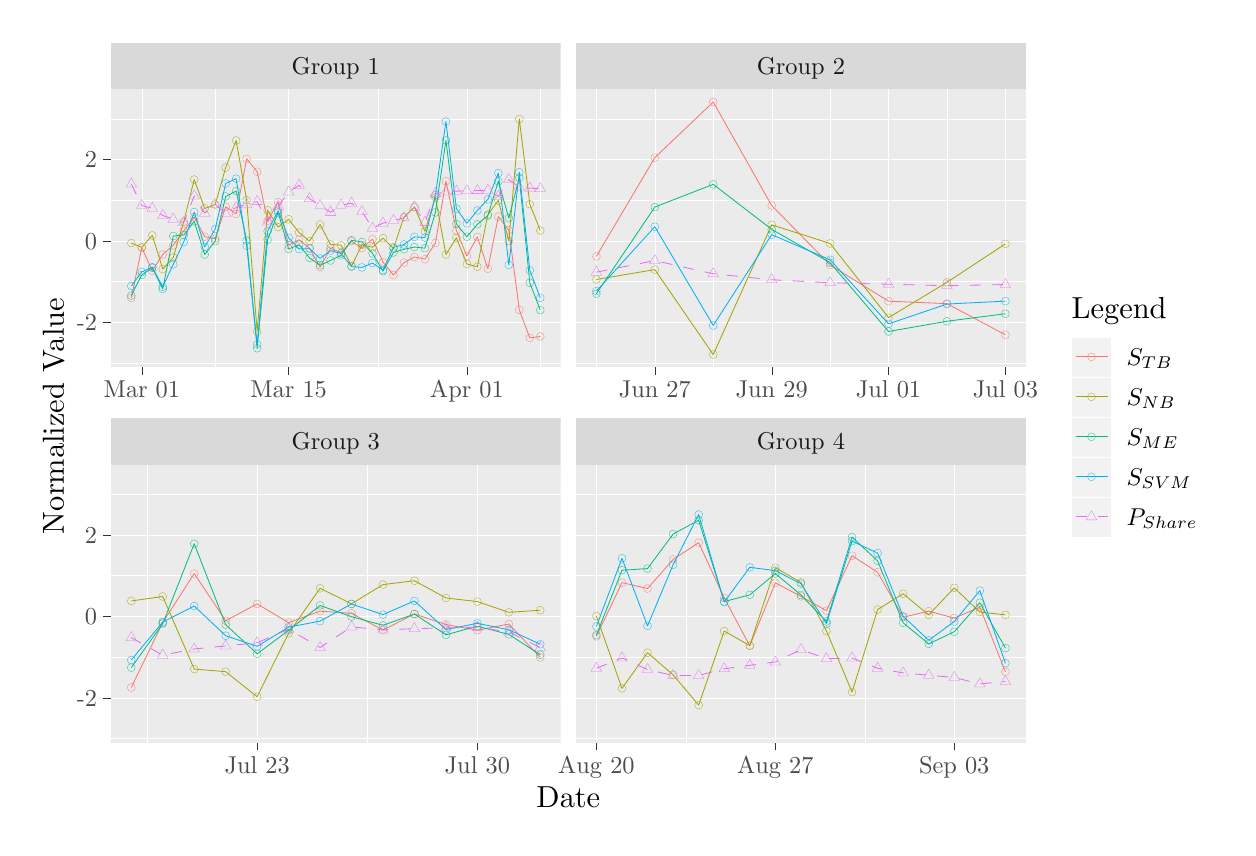
\begin{tikzpicture}[x=1pt,y=1pt]
\definecolor{fillColor}{RGB}{255,255,255}
\path[use as bounding box,fill=fillColor,fill opacity=0.00] (0,0) rectangle (433.62,289.08);
\begin{scope}
\path[clip] (  0.00,  0.00) rectangle (433.62,289.08);
\definecolor{drawColor}{RGB}{255,255,255}
\definecolor{fillColor}{RGB}{255,255,255}

\path[draw=drawColor,line width= 0.1pt,line join=round,line cap=round,fill=fillColor] (  0.00,  0.00) rectangle (433.62,289.08);
\end{scope}
\begin{scope}
\path[clip] ( 30.06,166.38) rectangle (192.62,266.77);
\definecolor{fillColor}{gray}{0.92}

\path[fill=fillColor] ( 30.06,166.38) rectangle (192.62,266.77);
\definecolor{drawColor}{RGB}{255,255,255}

\path[draw=drawColor,line width= 0.1pt,line join=round] ( 30.06,167.90) --
	(192.62,167.90);

\path[draw=drawColor,line width= 0.1pt,line join=round] ( 30.06,197.33) --
	(192.62,197.33);

\path[draw=drawColor,line width= 0.1pt,line join=round] ( 30.06,226.76) --
	(192.62,226.76);

\path[draw=drawColor,line width= 0.1pt,line join=round] ( 30.06,256.20) --
	(192.62,256.20);

\path[draw=drawColor,line width= 0.1pt,line join=round] ( 67.76,166.38) --
	( 67.76,266.77);

\path[draw=drawColor,line width= 0.1pt,line join=round] (126.50,166.38) --
	(126.50,266.77);

\path[draw=drawColor,line width= 0.1pt,line join=round] (185.23,166.38) --
	(185.23,266.77);

\path[draw=drawColor,line width= 0.1pt,line join=round] ( 30.06,182.62) --
	(192.62,182.62);

\path[draw=drawColor,line width= 0.1pt,line join=round] ( 30.06,212.05) --
	(192.62,212.05);

\path[draw=drawColor,line width= 0.1pt,line join=round] ( 30.06,241.48) --
	(192.62,241.48);

\path[draw=drawColor,line width= 0.1pt,line join=round] ( 41.23,166.38) --
	( 41.23,266.77);

\path[draw=drawColor,line width= 0.1pt,line join=round] ( 94.29,166.38) --
	( 94.29,266.77);

\path[draw=drawColor,line width= 0.1pt,line join=round] (158.71,166.38) --
	(158.71,266.77);
\definecolor{drawColor}{RGB}{248,118,109}

\path[draw=drawColor,line width= 0.3pt,line join=round] ( 37.44,191.42) --
	( 41.23,209.59) --
	( 45.02,201.23) --
	( 48.81,207.13) --
	( 52.60,210.44) --
	( 56.39,215.63) --
	( 60.18,220.64) --
	( 63.97,213.55) --
	( 67.76,212.85) --
	( 71.55,224.35) --
	( 75.34,221.79) --
	( 79.13,241.68) --
	( 82.92,237.02) --
	( 86.71,219.35) --
	( 90.50,226.01) --
	( 94.29,210.55) --
	( 98.08,212.45) --
	(101.86,209.41) --
	(105.65,202.53) --
	(109.44,209.36) --
	(113.23,207.69) --
	(117.02,211.93) --
	(120.81,209.45) --
	(124.60,212.65) --
	(128.39,204.37) --
	(132.18,199.69) --
	(135.97,204.19) --
	(139.76,206.22) --
	(143.55,205.44) --
	(147.34,211.27) --
	(151.13,233.62) --
	(154.92,215.74) --
	(158.71,206.58) --
	(162.49,213.48) --
	(166.28,201.98) --
	(170.07,220.82) --
	(173.86,215.92) --
	(177.65,187.12) --
	(181.44,176.98) --
	(185.23,177.49);
\definecolor{drawColor}{RGB}{163,165,0}

\path[draw=drawColor,line width= 0.3pt,line join=round] ( 37.44,211.24) --
	( 41.23,209.69) --
	( 45.02,214.02) --
	( 48.81,201.84) --
	( 52.60,206.00) --
	( 56.39,218.98) --
	( 60.18,234.20) --
	( 63.97,223.75) --
	( 67.76,225.16) --
	( 71.55,238.53) --
	( 75.34,248.32) --
	( 79.13,226.73) --
	( 82.92,179.35) --
	( 86.71,223.09) --
	( 90.50,217.02) --
	( 94.29,219.83) --
	( 98.08,215.07) --
	(101.86,211.96) --
	(105.65,217.97) --
	(109.44,210.75) --
	(113.23,210.51) --
	(117.02,202.91) --
	(120.81,210.58) --
	(124.60,209.75) --
	(128.39,213.02) --
	(132.18,209.29) --
	(135.97,220.67) --
	(139.76,224.24) --
	(143.55,215.49) --
	(147.34,227.75) --
	(151.13,207.11) --
	(154.92,213.14) --
	(158.71,203.68) --
	(162.49,202.70) --
	(166.28,221.50) --
	(170.07,226.65) --
	(173.86,211.98) --
	(177.65,256.08) --
	(181.44,225.32) --
	(185.23,215.78);
\definecolor{drawColor}{RGB}{0,191,125}

\path[draw=drawColor,line width= 0.3pt,line join=round] ( 37.44,192.30) --
	( 41.23,199.71) --
	( 45.02,202.31) --
	( 48.81,194.66) --
	( 52.60,213.79) --
	( 56.39,214.16) --
	( 60.18,219.11) --
	( 63.97,207.11) --
	( 67.76,211.96) --
	( 71.55,228.09) --
	( 75.34,230.04) --
	( 79.13,212.13) --
	( 82.92,173.23) --
	( 86.71,212.46) --
	( 90.50,222.32) --
	( 94.29,209.11) --
	( 98.08,210.64) --
	(101.86,205.85) --
	(105.65,203.25) --
	(109.44,204.96) --
	(113.23,206.82) --
	(117.02,212.27) --
	(120.81,211.64) --
	(124.60,207.52) --
	(128.39,201.10) --
	(132.18,207.85) --
	(135.97,209.00) --
	(139.76,209.79) --
	(143.55,209.41) --
	(147.34,222.33) --
	(151.13,248.34) --
	(154.92,218.15) --
	(158.71,213.53) --
	(162.49,218.03) --
	(166.28,221.16) --
	(170.07,233.59) --
	(173.86,220.26) --
	(177.65,234.81) --
	(181.44,196.90) --
	(185.23,187.02);
\definecolor{drawColor}{RGB}{0,176,246}

\path[draw=drawColor,line width= 0.3pt,line join=round] ( 37.44,195.74) --
	( 41.23,200.80) --
	( 45.02,202.52) --
	( 48.81,195.45) --
	( 52.60,203.54) --
	( 56.39,211.61) --
	( 60.18,222.45) --
	( 63.97,209.85) --
	( 67.76,216.32) --
	( 71.55,232.78) --
	( 75.34,234.51) --
	( 79.13,210.28) --
	( 82.92,174.63) --
	( 86.71,215.53) --
	( 90.50,222.90) --
	( 94.29,213.16) --
	( 98.08,209.08) --
	(101.86,209.24) --
	(105.65,205.70) --
	(109.44,208.51) --
	(113.23,207.47) --
	(117.02,202.74) --
	(120.81,202.44) --
	(124.60,204.02) --
	(128.39,201.49) --
	(132.18,209.68) --
	(135.97,210.72) --
	(139.76,213.48) --
	(143.55,213.25) --
	(147.34,228.56) --
	(151.13,255.15) --
	(154.92,223.70) --
	(158.71,218.38) --
	(162.49,223.03) --
	(166.28,227.02) --
	(170.07,236.52) --
	(173.86,203.34) --
	(177.65,236.85) --
	(181.44,201.39) --
	(185.23,191.44);
\definecolor{drawColor}{RGB}{231,107,243}

\path[draw=drawColor,line width= 0.3pt,dash pattern=on 4pt off 4pt ,line join=round] ( 37.44,232.59) --
	( 41.23,224.81) --
	( 45.02,223.80) --
	( 48.81,221.20) --
	( 52.60,219.91) --
	( 56.39,218.61) --
	( 60.18,228.27) --
	( 63.97,222.07) --
	( 67.76,225.24) --
	( 71.55,221.92) --
	( 75.34,224.09) --
	( 79.13,225.17) --
	( 82.92,226.25) --
	( 86.71,218.90) --
	( 90.50,224.52) --
	( 94.29,229.71) --
	( 98.08,232.16) --
	(101.86,227.26) --
	(105.65,224.81) --
	(109.44,222.36) --
	(113.23,224.95) --
	(117.02,225.67) --
	(120.81,222.65) --
	(124.60,216.59) --
	(128.39,218.46) --
	(132.18,219.40) --
	(135.97,220.34) --
	(139.76,224.23) --
	(143.55,218.75) --
	(147.34,229.13) --
	(151.13,229.71) --
	(154.92,230.00) --
	(158.71,230.14) --
	(162.49,230.22) --
	(166.28,230.29) --
	(170.07,228.12) --
	(173.86,234.18) --
	(177.65,231.44) --
	(181.44,231.08) --
	(185.23,230.90);
\definecolor{drawColor}{RGB}{248,118,109}

\path[draw=drawColor,line width= 0.1pt,line join=round,line cap=round] ( 37.44,191.42) circle (  1.43);

\path[draw=drawColor,line width= 0.1pt,line join=round,line cap=round] ( 41.23,209.59) circle (  1.43);

\path[draw=drawColor,line width= 0.1pt,line join=round,line cap=round] ( 45.02,201.23) circle (  1.43);

\path[draw=drawColor,line width= 0.1pt,line join=round,line cap=round] ( 48.81,207.13) circle (  1.43);

\path[draw=drawColor,line width= 0.1pt,line join=round,line cap=round] ( 52.60,210.44) circle (  1.43);

\path[draw=drawColor,line width= 0.1pt,line join=round,line cap=round] ( 56.39,215.63) circle (  1.43);

\path[draw=drawColor,line width= 0.1pt,line join=round,line cap=round] ( 60.18,220.64) circle (  1.43);

\path[draw=drawColor,line width= 0.1pt,line join=round,line cap=round] ( 63.97,213.55) circle (  1.43);

\path[draw=drawColor,line width= 0.1pt,line join=round,line cap=round] ( 67.76,212.85) circle (  1.43);

\path[draw=drawColor,line width= 0.1pt,line join=round,line cap=round] ( 71.55,224.35) circle (  1.43);

\path[draw=drawColor,line width= 0.1pt,line join=round,line cap=round] ( 75.34,221.79) circle (  1.43);

\path[draw=drawColor,line width= 0.1pt,line join=round,line cap=round] ( 79.13,241.68) circle (  1.43);

\path[draw=drawColor,line width= 0.1pt,line join=round,line cap=round] ( 82.92,237.02) circle (  1.43);

\path[draw=drawColor,line width= 0.1pt,line join=round,line cap=round] ( 86.71,219.35) circle (  1.43);

\path[draw=drawColor,line width= 0.1pt,line join=round,line cap=round] ( 90.50,226.01) circle (  1.43);

\path[draw=drawColor,line width= 0.1pt,line join=round,line cap=round] ( 94.29,210.55) circle (  1.43);

\path[draw=drawColor,line width= 0.1pt,line join=round,line cap=round] ( 98.08,212.45) circle (  1.43);

\path[draw=drawColor,line width= 0.1pt,line join=round,line cap=round] (101.86,209.41) circle (  1.43);

\path[draw=drawColor,line width= 0.1pt,line join=round,line cap=round] (105.65,202.53) circle (  1.43);

\path[draw=drawColor,line width= 0.1pt,line join=round,line cap=round] (109.44,209.36) circle (  1.43);

\path[draw=drawColor,line width= 0.1pt,line join=round,line cap=round] (113.23,207.69) circle (  1.43);

\path[draw=drawColor,line width= 0.1pt,line join=round,line cap=round] (117.02,211.93) circle (  1.43);

\path[draw=drawColor,line width= 0.1pt,line join=round,line cap=round] (120.81,209.45) circle (  1.43);

\path[draw=drawColor,line width= 0.1pt,line join=round,line cap=round] (124.60,212.65) circle (  1.43);

\path[draw=drawColor,line width= 0.1pt,line join=round,line cap=round] (128.39,204.37) circle (  1.43);

\path[draw=drawColor,line width= 0.1pt,line join=round,line cap=round] (132.18,199.69) circle (  1.43);

\path[draw=drawColor,line width= 0.1pt,line join=round,line cap=round] (135.97,204.19) circle (  1.43);

\path[draw=drawColor,line width= 0.1pt,line join=round,line cap=round] (139.76,206.22) circle (  1.43);

\path[draw=drawColor,line width= 0.1pt,line join=round,line cap=round] (143.55,205.44) circle (  1.43);

\path[draw=drawColor,line width= 0.1pt,line join=round,line cap=round] (147.34,211.27) circle (  1.43);

\path[draw=drawColor,line width= 0.1pt,line join=round,line cap=round] (151.13,233.62) circle (  1.43);

\path[draw=drawColor,line width= 0.1pt,line join=round,line cap=round] (154.92,215.74) circle (  1.43);

\path[draw=drawColor,line width= 0.1pt,line join=round,line cap=round] (158.71,206.58) circle (  1.43);

\path[draw=drawColor,line width= 0.1pt,line join=round,line cap=round] (162.49,213.48) circle (  1.43);

\path[draw=drawColor,line width= 0.1pt,line join=round,line cap=round] (166.28,201.98) circle (  1.43);

\path[draw=drawColor,line width= 0.1pt,line join=round,line cap=round] (170.07,220.82) circle (  1.43);

\path[draw=drawColor,line width= 0.1pt,line join=round,line cap=round] (173.86,215.92) circle (  1.43);

\path[draw=drawColor,line width= 0.1pt,line join=round,line cap=round] (177.65,187.12) circle (  1.43);

\path[draw=drawColor,line width= 0.1pt,line join=round,line cap=round] (181.44,176.98) circle (  1.43);

\path[draw=drawColor,line width= 0.1pt,line join=round,line cap=round] (185.23,177.49) circle (  1.43);
\definecolor{drawColor}{RGB}{163,165,0}

\path[draw=drawColor,line width= 0.1pt,line join=round,line cap=round] ( 37.44,211.24) circle (  1.43);

\path[draw=drawColor,line width= 0.1pt,line join=round,line cap=round] ( 41.23,209.69) circle (  1.43);

\path[draw=drawColor,line width= 0.1pt,line join=round,line cap=round] ( 45.02,214.02) circle (  1.43);

\path[draw=drawColor,line width= 0.1pt,line join=round,line cap=round] ( 48.81,201.84) circle (  1.43);

\path[draw=drawColor,line width= 0.1pt,line join=round,line cap=round] ( 52.60,206.00) circle (  1.43);

\path[draw=drawColor,line width= 0.1pt,line join=round,line cap=round] ( 56.39,218.98) circle (  1.43);

\path[draw=drawColor,line width= 0.1pt,line join=round,line cap=round] ( 60.18,234.20) circle (  1.43);

\path[draw=drawColor,line width= 0.1pt,line join=round,line cap=round] ( 63.97,223.75) circle (  1.43);

\path[draw=drawColor,line width= 0.1pt,line join=round,line cap=round] ( 67.76,225.16) circle (  1.43);

\path[draw=drawColor,line width= 0.1pt,line join=round,line cap=round] ( 71.55,238.53) circle (  1.43);

\path[draw=drawColor,line width= 0.1pt,line join=round,line cap=round] ( 75.34,248.32) circle (  1.43);

\path[draw=drawColor,line width= 0.1pt,line join=round,line cap=round] ( 79.13,226.73) circle (  1.43);

\path[draw=drawColor,line width= 0.1pt,line join=round,line cap=round] ( 82.92,179.35) circle (  1.43);

\path[draw=drawColor,line width= 0.1pt,line join=round,line cap=round] ( 86.71,223.09) circle (  1.43);

\path[draw=drawColor,line width= 0.1pt,line join=round,line cap=round] ( 90.50,217.02) circle (  1.43);

\path[draw=drawColor,line width= 0.1pt,line join=round,line cap=round] ( 94.29,219.83) circle (  1.43);

\path[draw=drawColor,line width= 0.1pt,line join=round,line cap=round] ( 98.08,215.07) circle (  1.43);

\path[draw=drawColor,line width= 0.1pt,line join=round,line cap=round] (101.86,211.96) circle (  1.43);

\path[draw=drawColor,line width= 0.1pt,line join=round,line cap=round] (105.65,217.97) circle (  1.43);

\path[draw=drawColor,line width= 0.1pt,line join=round,line cap=round] (109.44,210.75) circle (  1.43);

\path[draw=drawColor,line width= 0.1pt,line join=round,line cap=round] (113.23,210.51) circle (  1.43);

\path[draw=drawColor,line width= 0.1pt,line join=round,line cap=round] (117.02,202.91) circle (  1.43);

\path[draw=drawColor,line width= 0.1pt,line join=round,line cap=round] (120.81,210.58) circle (  1.43);

\path[draw=drawColor,line width= 0.1pt,line join=round,line cap=round] (124.60,209.75) circle (  1.43);

\path[draw=drawColor,line width= 0.1pt,line join=round,line cap=round] (128.39,213.02) circle (  1.43);

\path[draw=drawColor,line width= 0.1pt,line join=round,line cap=round] (132.18,209.29) circle (  1.43);

\path[draw=drawColor,line width= 0.1pt,line join=round,line cap=round] (135.97,220.67) circle (  1.43);

\path[draw=drawColor,line width= 0.1pt,line join=round,line cap=round] (139.76,224.24) circle (  1.43);

\path[draw=drawColor,line width= 0.1pt,line join=round,line cap=round] (143.55,215.49) circle (  1.43);

\path[draw=drawColor,line width= 0.1pt,line join=round,line cap=round] (147.34,227.75) circle (  1.43);

\path[draw=drawColor,line width= 0.1pt,line join=round,line cap=round] (151.13,207.11) circle (  1.43);

\path[draw=drawColor,line width= 0.1pt,line join=round,line cap=round] (154.92,213.14) circle (  1.43);

\path[draw=drawColor,line width= 0.1pt,line join=round,line cap=round] (158.71,203.68) circle (  1.43);

\path[draw=drawColor,line width= 0.1pt,line join=round,line cap=round] (162.49,202.70) circle (  1.43);

\path[draw=drawColor,line width= 0.1pt,line join=round,line cap=round] (166.28,221.50) circle (  1.43);

\path[draw=drawColor,line width= 0.1pt,line join=round,line cap=round] (170.07,226.65) circle (  1.43);

\path[draw=drawColor,line width= 0.1pt,line join=round,line cap=round] (173.86,211.98) circle (  1.43);

\path[draw=drawColor,line width= 0.1pt,line join=round,line cap=round] (177.65,256.08) circle (  1.43);

\path[draw=drawColor,line width= 0.1pt,line join=round,line cap=round] (181.44,225.32) circle (  1.43);

\path[draw=drawColor,line width= 0.1pt,line join=round,line cap=round] (185.23,215.78) circle (  1.43);
\definecolor{drawColor}{RGB}{0,191,125}

\path[draw=drawColor,line width= 0.1pt,line join=round,line cap=round] ( 37.44,192.30) circle (  1.43);

\path[draw=drawColor,line width= 0.1pt,line join=round,line cap=round] ( 41.23,199.71) circle (  1.43);

\path[draw=drawColor,line width= 0.1pt,line join=round,line cap=round] ( 45.02,202.31) circle (  1.43);

\path[draw=drawColor,line width= 0.1pt,line join=round,line cap=round] ( 48.81,194.66) circle (  1.43);

\path[draw=drawColor,line width= 0.1pt,line join=round,line cap=round] ( 52.60,213.79) circle (  1.43);

\path[draw=drawColor,line width= 0.1pt,line join=round,line cap=round] ( 56.39,214.16) circle (  1.43);

\path[draw=drawColor,line width= 0.1pt,line join=round,line cap=round] ( 60.18,219.11) circle (  1.43);

\path[draw=drawColor,line width= 0.1pt,line join=round,line cap=round] ( 63.97,207.11) circle (  1.43);

\path[draw=drawColor,line width= 0.1pt,line join=round,line cap=round] ( 67.76,211.96) circle (  1.43);

\path[draw=drawColor,line width= 0.1pt,line join=round,line cap=round] ( 71.55,228.09) circle (  1.43);

\path[draw=drawColor,line width= 0.1pt,line join=round,line cap=round] ( 75.34,230.04) circle (  1.43);

\path[draw=drawColor,line width= 0.1pt,line join=round,line cap=round] ( 79.13,212.13) circle (  1.43);

\path[draw=drawColor,line width= 0.1pt,line join=round,line cap=round] ( 82.92,173.23) circle (  1.43);

\path[draw=drawColor,line width= 0.1pt,line join=round,line cap=round] ( 86.71,212.46) circle (  1.43);

\path[draw=drawColor,line width= 0.1pt,line join=round,line cap=round] ( 90.50,222.32) circle (  1.43);

\path[draw=drawColor,line width= 0.1pt,line join=round,line cap=round] ( 94.29,209.11) circle (  1.43);

\path[draw=drawColor,line width= 0.1pt,line join=round,line cap=round] ( 98.08,210.64) circle (  1.43);

\path[draw=drawColor,line width= 0.1pt,line join=round,line cap=round] (101.86,205.85) circle (  1.43);

\path[draw=drawColor,line width= 0.1pt,line join=round,line cap=round] (105.65,203.25) circle (  1.43);

\path[draw=drawColor,line width= 0.1pt,line join=round,line cap=round] (109.44,204.96) circle (  1.43);

\path[draw=drawColor,line width= 0.1pt,line join=round,line cap=round] (113.23,206.82) circle (  1.43);

\path[draw=drawColor,line width= 0.1pt,line join=round,line cap=round] (117.02,212.27) circle (  1.43);

\path[draw=drawColor,line width= 0.1pt,line join=round,line cap=round] (120.81,211.64) circle (  1.43);

\path[draw=drawColor,line width= 0.1pt,line join=round,line cap=round] (124.60,207.52) circle (  1.43);

\path[draw=drawColor,line width= 0.1pt,line join=round,line cap=round] (128.39,201.10) circle (  1.43);

\path[draw=drawColor,line width= 0.1pt,line join=round,line cap=round] (132.18,207.85) circle (  1.43);

\path[draw=drawColor,line width= 0.1pt,line join=round,line cap=round] (135.97,209.00) circle (  1.43);

\path[draw=drawColor,line width= 0.1pt,line join=round,line cap=round] (139.76,209.79) circle (  1.43);

\path[draw=drawColor,line width= 0.1pt,line join=round,line cap=round] (143.55,209.41) circle (  1.43);

\path[draw=drawColor,line width= 0.1pt,line join=round,line cap=round] (147.34,222.33) circle (  1.43);

\path[draw=drawColor,line width= 0.1pt,line join=round,line cap=round] (151.13,248.34) circle (  1.43);

\path[draw=drawColor,line width= 0.1pt,line join=round,line cap=round] (154.92,218.15) circle (  1.43);

\path[draw=drawColor,line width= 0.1pt,line join=round,line cap=round] (158.71,213.53) circle (  1.43);

\path[draw=drawColor,line width= 0.1pt,line join=round,line cap=round] (162.49,218.03) circle (  1.43);

\path[draw=drawColor,line width= 0.1pt,line join=round,line cap=round] (166.28,221.16) circle (  1.43);

\path[draw=drawColor,line width= 0.1pt,line join=round,line cap=round] (170.07,233.59) circle (  1.43);

\path[draw=drawColor,line width= 0.1pt,line join=round,line cap=round] (173.86,220.26) circle (  1.43);

\path[draw=drawColor,line width= 0.1pt,line join=round,line cap=round] (177.65,234.81) circle (  1.43);

\path[draw=drawColor,line width= 0.1pt,line join=round,line cap=round] (181.44,196.90) circle (  1.43);

\path[draw=drawColor,line width= 0.1pt,line join=round,line cap=round] (185.23,187.02) circle (  1.43);
\definecolor{drawColor}{RGB}{0,176,246}

\path[draw=drawColor,line width= 0.1pt,line join=round,line cap=round] ( 37.44,195.74) circle (  1.43);

\path[draw=drawColor,line width= 0.1pt,line join=round,line cap=round] ( 41.23,200.80) circle (  1.43);

\path[draw=drawColor,line width= 0.1pt,line join=round,line cap=round] ( 45.02,202.52) circle (  1.43);

\path[draw=drawColor,line width= 0.1pt,line join=round,line cap=round] ( 48.81,195.45) circle (  1.43);

\path[draw=drawColor,line width= 0.1pt,line join=round,line cap=round] ( 52.60,203.54) circle (  1.43);

\path[draw=drawColor,line width= 0.1pt,line join=round,line cap=round] ( 56.39,211.61) circle (  1.43);

\path[draw=drawColor,line width= 0.1pt,line join=round,line cap=round] ( 60.18,222.45) circle (  1.43);

\path[draw=drawColor,line width= 0.1pt,line join=round,line cap=round] ( 63.97,209.85) circle (  1.43);

\path[draw=drawColor,line width= 0.1pt,line join=round,line cap=round] ( 67.76,216.32) circle (  1.43);

\path[draw=drawColor,line width= 0.1pt,line join=round,line cap=round] ( 71.55,232.78) circle (  1.43);

\path[draw=drawColor,line width= 0.1pt,line join=round,line cap=round] ( 75.34,234.51) circle (  1.43);

\path[draw=drawColor,line width= 0.1pt,line join=round,line cap=round] ( 79.13,210.28) circle (  1.43);

\path[draw=drawColor,line width= 0.1pt,line join=round,line cap=round] ( 82.92,174.63) circle (  1.43);

\path[draw=drawColor,line width= 0.1pt,line join=round,line cap=round] ( 86.71,215.53) circle (  1.43);

\path[draw=drawColor,line width= 0.1pt,line join=round,line cap=round] ( 90.50,222.90) circle (  1.43);

\path[draw=drawColor,line width= 0.1pt,line join=round,line cap=round] ( 94.29,213.16) circle (  1.43);

\path[draw=drawColor,line width= 0.1pt,line join=round,line cap=round] ( 98.08,209.08) circle (  1.43);

\path[draw=drawColor,line width= 0.1pt,line join=round,line cap=round] (101.86,209.24) circle (  1.43);

\path[draw=drawColor,line width= 0.1pt,line join=round,line cap=round] (105.65,205.70) circle (  1.43);

\path[draw=drawColor,line width= 0.1pt,line join=round,line cap=round] (109.44,208.51) circle (  1.43);

\path[draw=drawColor,line width= 0.1pt,line join=round,line cap=round] (113.23,207.47) circle (  1.43);

\path[draw=drawColor,line width= 0.1pt,line join=round,line cap=round] (117.02,202.74) circle (  1.43);

\path[draw=drawColor,line width= 0.1pt,line join=round,line cap=round] (120.81,202.44) circle (  1.43);

\path[draw=drawColor,line width= 0.1pt,line join=round,line cap=round] (124.60,204.02) circle (  1.43);

\path[draw=drawColor,line width= 0.1pt,line join=round,line cap=round] (128.39,201.49) circle (  1.43);

\path[draw=drawColor,line width= 0.1pt,line join=round,line cap=round] (132.18,209.68) circle (  1.43);

\path[draw=drawColor,line width= 0.1pt,line join=round,line cap=round] (135.97,210.72) circle (  1.43);

\path[draw=drawColor,line width= 0.1pt,line join=round,line cap=round] (139.76,213.48) circle (  1.43);

\path[draw=drawColor,line width= 0.1pt,line join=round,line cap=round] (143.55,213.25) circle (  1.43);

\path[draw=drawColor,line width= 0.1pt,line join=round,line cap=round] (147.34,228.56) circle (  1.43);

\path[draw=drawColor,line width= 0.1pt,line join=round,line cap=round] (151.13,255.15) circle (  1.43);

\path[draw=drawColor,line width= 0.1pt,line join=round,line cap=round] (154.92,223.70) circle (  1.43);

\path[draw=drawColor,line width= 0.1pt,line join=round,line cap=round] (158.71,218.38) circle (  1.43);

\path[draw=drawColor,line width= 0.1pt,line join=round,line cap=round] (162.49,223.03) circle (  1.43);

\path[draw=drawColor,line width= 0.1pt,line join=round,line cap=round] (166.28,227.02) circle (  1.43);

\path[draw=drawColor,line width= 0.1pt,line join=round,line cap=round] (170.07,236.52) circle (  1.43);

\path[draw=drawColor,line width= 0.1pt,line join=round,line cap=round] (173.86,203.34) circle (  1.43);

\path[draw=drawColor,line width= 0.1pt,line join=round,line cap=round] (177.65,236.85) circle (  1.43);

\path[draw=drawColor,line width= 0.1pt,line join=round,line cap=round] (181.44,201.39) circle (  1.43);

\path[draw=drawColor,line width= 0.1pt,line join=round,line cap=round] (185.23,191.44) circle (  1.43);
\definecolor{drawColor}{RGB}{231,107,243}

\path[draw=drawColor,line width= 0.1pt,line join=round,line cap=round] ( 37.44,234.81) --
	( 39.37,231.49) --
	( 35.52,231.49) --
	( 37.44,234.81);

\path[draw=drawColor,line width= 0.1pt,line join=round,line cap=round] ( 41.23,227.03) --
	( 43.16,223.70) --
	( 39.31,223.70) --
	( 41.23,227.03);

\path[draw=drawColor,line width= 0.1pt,line join=round,line cap=round] ( 45.02,226.02) --
	( 46.94,222.69) --
	( 43.10,222.69) --
	( 45.02,226.02);

\path[draw=drawColor,line width= 0.1pt,line join=round,line cap=round] ( 48.81,223.42) --
	( 50.73,220.09) --
	( 46.89,220.09) --
	( 48.81,223.42);

\path[draw=drawColor,line width= 0.1pt,line join=round,line cap=round] ( 52.60,222.12) --
	( 54.52,218.80) --
	( 50.68,218.80) --
	( 52.60,222.12);

\path[draw=drawColor,line width= 0.1pt,line join=round,line cap=round] ( 56.39,220.83) --
	( 58.31,217.50) --
	( 54.47,217.50) --
	( 56.39,220.83);

\path[draw=drawColor,line width= 0.1pt,line join=round,line cap=round] ( 60.18,230.49) --
	( 62.10,227.16) --
	( 58.26,227.16) --
	( 60.18,230.49);

\path[draw=drawColor,line width= 0.1pt,line join=round,line cap=round] ( 63.97,224.29) --
	( 65.89,220.96) --
	( 62.05,220.96) --
	( 63.97,224.29);

\path[draw=drawColor,line width= 0.1pt,line join=round,line cap=round] ( 67.76,227.46) --
	( 69.68,224.13) --
	( 65.84,224.13) --
	( 67.76,227.46);

\path[draw=drawColor,line width= 0.1pt,line join=round,line cap=round] ( 71.55,224.14) --
	( 73.47,220.82) --
	( 69.63,220.82) --
	( 71.55,224.14);

\path[draw=drawColor,line width= 0.1pt,line join=round,line cap=round] ( 75.34,226.31) --
	( 77.26,222.98) --
	( 73.42,222.98) --
	( 75.34,226.31);

\path[draw=drawColor,line width= 0.1pt,line join=round,line cap=round] ( 79.13,227.39) --
	( 81.05,224.06) --
	( 77.21,224.06) --
	( 79.13,227.39);

\path[draw=drawColor,line width= 0.1pt,line join=round,line cap=round] ( 82.92,228.47) --
	( 84.84,225.14) --
	( 81.00,225.14) --
	( 82.92,228.47);

\path[draw=drawColor,line width= 0.1pt,line join=round,line cap=round] ( 86.71,221.12) --
	( 88.63,217.79) --
	( 84.79,217.79) --
	( 86.71,221.12);

\path[draw=drawColor,line width= 0.1pt,line join=round,line cap=round] ( 90.50,226.74) --
	( 92.42,223.41) --
	( 88.57,223.41) --
	( 90.50,226.74);

\path[draw=drawColor,line width= 0.1pt,line join=round,line cap=round] ( 94.29,231.93) --
	( 96.21,228.60) --
	( 92.36,228.60) --
	( 94.29,231.93);

\path[draw=drawColor,line width= 0.1pt,line join=round,line cap=round] ( 98.08,234.38) --
	(100.00,231.05) --
	( 96.15,231.05) --
	( 98.08,234.38);

\path[draw=drawColor,line width= 0.1pt,line join=round,line cap=round] (101.86,229.48) --
	(103.79,226.15) --
	( 99.94,226.15) --
	(101.86,229.48);

\path[draw=drawColor,line width= 0.1pt,line join=round,line cap=round] (105.65,227.03) --
	(107.58,223.70) --
	(103.73,223.70) --
	(105.65,227.03);

\path[draw=drawColor,line width= 0.1pt,line join=round,line cap=round] (109.44,224.58) --
	(111.36,221.25) --
	(107.52,221.25) --
	(109.44,224.58);

\path[draw=drawColor,line width= 0.1pt,line join=round,line cap=round] (113.23,227.17) --
	(115.15,223.84) --
	(111.31,223.84) --
	(113.23,227.17);

\path[draw=drawColor,line width= 0.1pt,line join=round,line cap=round] (117.02,227.89) --
	(118.94,224.56) --
	(115.10,224.56) --
	(117.02,227.89);

\path[draw=drawColor,line width= 0.1pt,line join=round,line cap=round] (120.81,224.86) --
	(122.73,221.54) --
	(118.89,221.54) --
	(120.81,224.86);

\path[draw=drawColor,line width= 0.1pt,line join=round,line cap=round] (124.60,218.81) --
	(126.52,215.48) --
	(122.68,215.48) --
	(124.60,218.81);

\path[draw=drawColor,line width= 0.1pt,line join=round,line cap=round] (128.39,220.68) --
	(130.31,217.35) --
	(126.47,217.35) --
	(128.39,220.68);

\path[draw=drawColor,line width= 0.1pt,line join=round,line cap=round] (132.18,221.62) --
	(134.10,218.29) --
	(130.26,218.29) --
	(132.18,221.62);

\path[draw=drawColor,line width= 0.1pt,line join=round,line cap=round] (135.97,222.56) --
	(137.89,219.23) --
	(134.05,219.23) --
	(135.97,222.56);

\path[draw=drawColor,line width= 0.1pt,line join=round,line cap=round] (139.76,226.45) --
	(141.68,223.12) --
	(137.84,223.12) --
	(139.76,226.45);

\path[draw=drawColor,line width= 0.1pt,line join=round,line cap=round] (143.55,220.97) --
	(145.47,217.64) --
	(141.63,217.64) --
	(143.55,220.97);

\path[draw=drawColor,line width= 0.1pt,line join=round,line cap=round] (147.34,231.35) --
	(149.26,228.02) --
	(145.42,228.02) --
	(147.34,231.35);

\path[draw=drawColor,line width= 0.1pt,line join=round,line cap=round] (151.13,231.93) --
	(153.05,228.60) --
	(149.21,228.60) --
	(151.13,231.93);

\path[draw=drawColor,line width= 0.1pt,line join=round,line cap=round] (154.92,232.22) --
	(156.84,228.89) --
	(152.99,228.89) --
	(154.92,232.22);

\path[draw=drawColor,line width= 0.1pt,line join=round,line cap=round] (158.71,232.36) --
	(160.63,229.03) --
	(156.78,229.03) --
	(158.71,232.36);

\path[draw=drawColor,line width= 0.1pt,line join=round,line cap=round] (162.49,232.43) --
	(164.42,229.11) --
	(160.57,229.11) --
	(162.49,232.43);

\path[draw=drawColor,line width= 0.1pt,line join=round,line cap=round] (166.28,232.51) --
	(168.21,229.18) --
	(164.36,229.18) --
	(166.28,232.51);

\path[draw=drawColor,line width= 0.1pt,line join=round,line cap=round] (170.07,230.34) --
	(171.99,227.02) --
	(168.15,227.02) --
	(170.07,230.34);

\path[draw=drawColor,line width= 0.1pt,line join=round,line cap=round] (173.86,236.40) --
	(175.78,233.07) --
	(171.94,233.07) --
	(173.86,236.40);

\path[draw=drawColor,line width= 0.1pt,line join=round,line cap=round] (177.65,233.66) --
	(179.57,230.33) --
	(175.73,230.33) --
	(177.65,233.66);

\path[draw=drawColor,line width= 0.1pt,line join=round,line cap=round] (181.44,233.30) --
	(183.36,229.97) --
	(179.52,229.97) --
	(181.44,233.30);

\path[draw=drawColor,line width= 0.1pt,line join=round,line cap=round] (185.23,233.12) --
	(187.15,229.79) --
	(183.31,229.79) --
	(185.23,233.12);
\end{scope}
\begin{scope}
\path[clip] ( 30.06, 30.73) rectangle (192.62,131.12);
\definecolor{fillColor}{gray}{0.92}

\path[fill=fillColor] ( 30.06, 30.73) rectangle (192.62,131.12);
\definecolor{drawColor}{RGB}{255,255,255}

\path[draw=drawColor,line width= 0.1pt,line join=round] ( 30.06, 32.25) --
	(192.62, 32.25);

\path[draw=drawColor,line width= 0.1pt,line join=round] ( 30.06, 61.68) --
	(192.62, 61.68);

\path[draw=drawColor,line width= 0.1pt,line join=round] ( 30.06, 91.11) --
	(192.62, 91.11);

\path[draw=drawColor,line width= 0.1pt,line join=round] ( 30.06,120.54) --
	(192.62,120.54);

\path[draw=drawColor,line width= 0.1pt,line join=round] ( 43.13, 30.73) --
	( 43.13,131.12);

\path[draw=drawColor,line width= 0.1pt,line join=round] (122.71, 30.73) --
	(122.71,131.12);

\path[draw=drawColor,line width= 0.1pt,line join=round] ( 30.06, 46.96) --
	(192.62, 46.96);

\path[draw=drawColor,line width= 0.1pt,line join=round] ( 30.06, 76.39) --
	(192.62, 76.39);

\path[draw=drawColor,line width= 0.1pt,line join=round] ( 30.06,105.83) --
	(192.62,105.83);

\path[draw=drawColor,line width= 0.1pt,line join=round] ( 82.92, 30.73) --
	( 82.92,131.12);

\path[draw=drawColor,line width= 0.1pt,line join=round] (162.49, 30.73) --
	(162.49,131.12);
\definecolor{drawColor}{RGB}{248,118,109}

\path[draw=drawColor,line width= 0.3pt,line join=round] ( 37.44, 50.67) --
	( 48.81, 74.13) --
	( 60.18, 91.82) --
	( 71.55, 74.77) --
	( 82.92, 80.87) --
	( 94.29, 74.09) --
	(105.65, 78.23) --
	(117.02, 77.48) --
	(128.39, 71.40) --
	(139.76, 77.22) --
	(151.13, 73.40) --
	(162.49, 71.34) --
	(173.86, 73.59) --
	(185.23, 61.53);
\definecolor{drawColor}{RGB}{163,165,0}

\path[draw=drawColor,line width= 0.3pt,line join=round] ( 37.44, 81.92) --
	( 48.81, 83.54) --
	( 60.18, 57.31) --
	( 71.55, 56.36) --
	( 82.92, 47.30) --
	( 94.29, 70.25) --
	(105.65, 86.50) --
	(117.02, 80.89) --
	(128.39, 87.84) --
	(139.76, 89.23) --
	(151.13, 83.01) --
	(162.49, 81.70) --
	(173.86, 77.82) --
	(185.23, 78.57);
\definecolor{drawColor}{RGB}{0,191,125}

\path[draw=drawColor,line width= 0.3pt,line join=round] ( 37.44, 57.82) --
	( 48.81, 73.72) --
	( 60.18,102.60) --
	( 71.55, 73.35) --
	( 82.92, 62.82) --
	( 94.29, 71.30) --
	(105.65, 80.29) --
	(117.02, 76.23) --
	(128.39, 73.12) --
	(139.76, 77.20) --
	(151.13, 69.68) --
	(162.49, 72.82) --
	(173.86, 69.84) --
	(185.23, 62.49);
\definecolor{drawColor}{RGB}{0,176,246}

\path[draw=drawColor,line width= 0.3pt,line join=round] ( 37.44, 60.59) --
	( 48.81, 74.31) --
	( 60.18, 80.08) --
	( 71.55, 69.36) --
	( 82.92, 65.53) --
	( 94.29, 72.46) --
	(105.65, 74.63) --
	(117.02, 80.82) --
	(128.39, 76.99) --
	(139.76, 81.94) --
	(151.13, 71.59) --
	(162.49, 73.84) --
	(173.86, 71.51) --
	(185.23, 66.29);
\definecolor{drawColor}{RGB}{231,107,243}

\path[draw=drawColor,line width= 0.3pt,dash pattern=on 4pt off 4pt ,line join=round] ( 37.44, 68.68) --
	( 48.81, 62.34) --
	( 60.18, 64.57) --
	( 71.55, 65.69) --
	( 82.92, 66.81) --
	( 94.29, 71.71) --
	(105.65, 65.08) --
	(117.02, 72.57) --
	(128.39, 71.42) --
	(139.76, 71.92) --
	(151.13, 72.18) --
	(162.49, 72.43) --
	(173.86, 70.70) --
	(185.23, 65.08);
\definecolor{drawColor}{RGB}{248,118,109}

\path[draw=drawColor,line width= 0.1pt,line join=round,line cap=round] ( 37.44, 50.67) circle (  1.43);

\path[draw=drawColor,line width= 0.1pt,line join=round,line cap=round] ( 48.81, 74.13) circle (  1.43);

\path[draw=drawColor,line width= 0.1pt,line join=round,line cap=round] ( 60.18, 91.82) circle (  1.43);

\path[draw=drawColor,line width= 0.1pt,line join=round,line cap=round] ( 71.55, 74.77) circle (  1.43);

\path[draw=drawColor,line width= 0.1pt,line join=round,line cap=round] ( 82.92, 80.87) circle (  1.43);

\path[draw=drawColor,line width= 0.1pt,line join=round,line cap=round] ( 94.29, 74.09) circle (  1.43);

\path[draw=drawColor,line width= 0.1pt,line join=round,line cap=round] (105.65, 78.23) circle (  1.43);

\path[draw=drawColor,line width= 0.1pt,line join=round,line cap=round] (117.02, 77.48) circle (  1.43);

\path[draw=drawColor,line width= 0.1pt,line join=round,line cap=round] (128.39, 71.40) circle (  1.43);

\path[draw=drawColor,line width= 0.1pt,line join=round,line cap=round] (139.76, 77.22) circle (  1.43);

\path[draw=drawColor,line width= 0.1pt,line join=round,line cap=round] (151.13, 73.40) circle (  1.43);

\path[draw=drawColor,line width= 0.1pt,line join=round,line cap=round] (162.49, 71.34) circle (  1.43);

\path[draw=drawColor,line width= 0.1pt,line join=round,line cap=round] (173.86, 73.59) circle (  1.43);

\path[draw=drawColor,line width= 0.1pt,line join=round,line cap=round] (185.23, 61.53) circle (  1.43);
\definecolor{drawColor}{RGB}{163,165,0}

\path[draw=drawColor,line width= 0.1pt,line join=round,line cap=round] ( 37.44, 81.92) circle (  1.43);

\path[draw=drawColor,line width= 0.1pt,line join=round,line cap=round] ( 48.81, 83.54) circle (  1.43);

\path[draw=drawColor,line width= 0.1pt,line join=round,line cap=round] ( 60.18, 57.31) circle (  1.43);

\path[draw=drawColor,line width= 0.1pt,line join=round,line cap=round] ( 71.55, 56.36) circle (  1.43);

\path[draw=drawColor,line width= 0.1pt,line join=round,line cap=round] ( 82.92, 47.30) circle (  1.43);

\path[draw=drawColor,line width= 0.1pt,line join=round,line cap=round] ( 94.29, 70.25) circle (  1.43);

\path[draw=drawColor,line width= 0.1pt,line join=round,line cap=round] (105.65, 86.50) circle (  1.43);

\path[draw=drawColor,line width= 0.1pt,line join=round,line cap=round] (117.02, 80.89) circle (  1.43);

\path[draw=drawColor,line width= 0.1pt,line join=round,line cap=round] (128.39, 87.84) circle (  1.43);

\path[draw=drawColor,line width= 0.1pt,line join=round,line cap=round] (139.76, 89.23) circle (  1.43);

\path[draw=drawColor,line width= 0.1pt,line join=round,line cap=round] (151.13, 83.01) circle (  1.43);

\path[draw=drawColor,line width= 0.1pt,line join=round,line cap=round] (162.49, 81.70) circle (  1.43);

\path[draw=drawColor,line width= 0.1pt,line join=round,line cap=round] (173.86, 77.82) circle (  1.43);

\path[draw=drawColor,line width= 0.1pt,line join=round,line cap=round] (185.23, 78.57) circle (  1.43);
\definecolor{drawColor}{RGB}{0,191,125}

\path[draw=drawColor,line width= 0.1pt,line join=round,line cap=round] ( 37.44, 57.82) circle (  1.43);

\path[draw=drawColor,line width= 0.1pt,line join=round,line cap=round] ( 48.81, 73.72) circle (  1.43);

\path[draw=drawColor,line width= 0.1pt,line join=round,line cap=round] ( 60.18,102.60) circle (  1.43);

\path[draw=drawColor,line width= 0.1pt,line join=round,line cap=round] ( 71.55, 73.35) circle (  1.43);

\path[draw=drawColor,line width= 0.1pt,line join=round,line cap=round] ( 82.92, 62.82) circle (  1.43);

\path[draw=drawColor,line width= 0.1pt,line join=round,line cap=round] ( 94.29, 71.30) circle (  1.43);

\path[draw=drawColor,line width= 0.1pt,line join=round,line cap=round] (105.65, 80.29) circle (  1.43);

\path[draw=drawColor,line width= 0.1pt,line join=round,line cap=round] (117.02, 76.23) circle (  1.43);

\path[draw=drawColor,line width= 0.1pt,line join=round,line cap=round] (128.39, 73.12) circle (  1.43);

\path[draw=drawColor,line width= 0.1pt,line join=round,line cap=round] (139.76, 77.20) circle (  1.43);

\path[draw=drawColor,line width= 0.1pt,line join=round,line cap=round] (151.13, 69.68) circle (  1.43);

\path[draw=drawColor,line width= 0.1pt,line join=round,line cap=round] (162.49, 72.82) circle (  1.43);

\path[draw=drawColor,line width= 0.1pt,line join=round,line cap=round] (173.86, 69.84) circle (  1.43);

\path[draw=drawColor,line width= 0.1pt,line join=round,line cap=round] (185.23, 62.49) circle (  1.43);
\definecolor{drawColor}{RGB}{0,176,246}

\path[draw=drawColor,line width= 0.1pt,line join=round,line cap=round] ( 37.44, 60.59) circle (  1.43);

\path[draw=drawColor,line width= 0.1pt,line join=round,line cap=round] ( 48.81, 74.31) circle (  1.43);

\path[draw=drawColor,line width= 0.1pt,line join=round,line cap=round] ( 60.18, 80.08) circle (  1.43);

\path[draw=drawColor,line width= 0.1pt,line join=round,line cap=round] ( 71.55, 69.36) circle (  1.43);

\path[draw=drawColor,line width= 0.1pt,line join=round,line cap=round] ( 82.92, 65.53) circle (  1.43);

\path[draw=drawColor,line width= 0.1pt,line join=round,line cap=round] ( 94.29, 72.46) circle (  1.43);

\path[draw=drawColor,line width= 0.1pt,line join=round,line cap=round] (105.65, 74.63) circle (  1.43);

\path[draw=drawColor,line width= 0.1pt,line join=round,line cap=round] (117.02, 80.82) circle (  1.43);

\path[draw=drawColor,line width= 0.1pt,line join=round,line cap=round] (128.39, 76.99) circle (  1.43);

\path[draw=drawColor,line width= 0.1pt,line join=round,line cap=round] (139.76, 81.94) circle (  1.43);

\path[draw=drawColor,line width= 0.1pt,line join=round,line cap=round] (151.13, 71.59) circle (  1.43);

\path[draw=drawColor,line width= 0.1pt,line join=round,line cap=round] (162.49, 73.84) circle (  1.43);

\path[draw=drawColor,line width= 0.1pt,line join=round,line cap=round] (173.86, 71.51) circle (  1.43);

\path[draw=drawColor,line width= 0.1pt,line join=round,line cap=round] (185.23, 66.29) circle (  1.43);
\definecolor{drawColor}{RGB}{231,107,243}

\path[draw=drawColor,line width= 0.1pt,line join=round,line cap=round] ( 37.44, 70.90) --
	( 39.37, 67.57) --
	( 35.52, 67.57) --
	( 37.44, 70.90);

\path[draw=drawColor,line width= 0.1pt,line join=round,line cap=round] ( 48.81, 64.55) --
	( 50.73, 61.23) --
	( 46.89, 61.23) --
	( 48.81, 64.55);

\path[draw=drawColor,line width= 0.1pt,line join=round,line cap=round] ( 60.18, 66.79) --
	( 62.10, 63.46) --
	( 58.26, 63.46) --
	( 60.18, 66.79);

\path[draw=drawColor,line width= 0.1pt,line join=round,line cap=round] ( 71.55, 67.91) --
	( 73.47, 64.58) --
	( 69.63, 64.58) --
	( 71.55, 67.91);

\path[draw=drawColor,line width= 0.1pt,line join=round,line cap=round] ( 82.92, 69.02) --
	( 84.84, 65.70) --
	( 81.00, 65.70) --
	( 82.92, 69.02);

\path[draw=drawColor,line width= 0.1pt,line join=round,line cap=round] ( 94.29, 73.93) --
	( 96.21, 70.60) --
	( 92.36, 70.60) --
	( 94.29, 73.93);

\path[draw=drawColor,line width= 0.1pt,line join=round,line cap=round] (105.65, 67.29) --
	(107.58, 63.97) --
	(103.73, 63.97) --
	(105.65, 67.29);

\path[draw=drawColor,line width= 0.1pt,line join=round,line cap=round] (117.02, 74.79) --
	(118.94, 71.46) --
	(115.10, 71.46) --
	(117.02, 74.79);

\path[draw=drawColor,line width= 0.1pt,line join=round,line cap=round] (128.39, 73.64) --
	(130.31, 70.31) --
	(126.47, 70.31) --
	(128.39, 73.64);

\path[draw=drawColor,line width= 0.1pt,line join=round,line cap=round] (139.76, 74.14) --
	(141.68, 70.81) --
	(137.84, 70.81) --
	(139.76, 74.14);

\path[draw=drawColor,line width= 0.1pt,line join=round,line cap=round] (151.13, 74.39) --
	(153.05, 71.07) --
	(149.21, 71.07) --
	(151.13, 74.39);

\path[draw=drawColor,line width= 0.1pt,line join=round,line cap=round] (162.49, 74.65) --
	(164.42, 71.32) --
	(160.57, 71.32) --
	(162.49, 74.65);

\path[draw=drawColor,line width= 0.1pt,line join=round,line cap=round] (173.86, 72.92) --
	(175.78, 69.59) --
	(171.94, 69.59) --
	(173.86, 72.92);

\path[draw=drawColor,line width= 0.1pt,line join=round,line cap=round] (185.23, 67.29) --
	(187.15, 63.97) --
	(183.31, 63.97) --
	(185.23, 67.29);
\end{scope}
\begin{scope}
\path[clip] (198.12,166.38) rectangle (360.69,266.77);
\definecolor{fillColor}{gray}{0.92}

\path[fill=fillColor] (198.12,166.38) rectangle (360.69,266.77);
\definecolor{drawColor}{RGB}{255,255,255}

\path[draw=drawColor,line width= 0.1pt,line join=round] (198.12,167.90) --
	(360.69,167.90);

\path[draw=drawColor,line width= 0.1pt,line join=round] (198.12,197.33) --
	(360.69,197.33);

\path[draw=drawColor,line width= 0.1pt,line join=round] (198.12,226.76) --
	(360.69,226.76);

\path[draw=drawColor,line width= 0.1pt,line join=round] (198.12,256.20) --
	(360.69,256.20);

\path[draw=drawColor,line width= 0.1pt,line join=round] (205.51,166.38) --
	(205.51,266.77);

\path[draw=drawColor,line width= 0.1pt,line join=round] (247.73,166.38) --
	(247.73,266.77);

\path[draw=drawColor,line width= 0.1pt,line join=round] (289.96,166.38) --
	(289.96,266.77);

\path[draw=drawColor,line width= 0.1pt,line join=round] (332.18,166.38) --
	(332.18,266.77);

\path[draw=drawColor,line width= 0.1pt,line join=round] (198.12,182.62) --
	(360.69,182.62);

\path[draw=drawColor,line width= 0.1pt,line join=round] (198.12,212.05) --
	(360.69,212.05);

\path[draw=drawColor,line width= 0.1pt,line join=round] (198.12,241.48) --
	(360.69,241.48);

\path[draw=drawColor,line width= 0.1pt,line join=round] (226.62,166.38) --
	(226.62,266.77);

\path[draw=drawColor,line width= 0.1pt,line join=round] (268.85,166.38) --
	(268.85,266.77);

\path[draw=drawColor,line width= 0.1pt,line join=round] (311.07,166.38) --
	(311.07,266.77);

\path[draw=drawColor,line width= 0.1pt,line join=round] (353.30,166.38) --
	(353.30,266.77);
\definecolor{drawColor}{RGB}{248,118,109}

\path[draw=drawColor,line width= 0.3pt,line join=round] (205.51,206.44) --
	(226.62,242.12) --
	(247.73,262.21) --
	(268.85,224.81) --
	(289.96,203.31) --
	(311.07,190.25) --
	(332.18,189.36) --
	(353.30,178.09);
\definecolor{drawColor}{RGB}{163,165,0}

\path[draw=drawColor,line width= 0.3pt,line join=round] (205.51,198.09) --
	(226.62,201.65) --
	(247.73,170.95) --
	(268.85,217.83) --
	(289.96,211.10) --
	(311.07,184.30) --
	(332.18,197.06) --
	(353.30,210.96);
\definecolor{drawColor}{RGB}{0,191,125}

\path[draw=drawColor,line width= 0.3pt,line join=round] (205.51,192.96) --
	(226.62,224.26) --
	(247.73,232.47) --
	(268.85,216.20) --
	(289.96,204.16) --
	(311.07,179.29) --
	(332.18,183.00) --
	(353.30,185.70);
\definecolor{drawColor}{RGB}{0,176,246}

\path[draw=drawColor,line width= 0.3pt,line join=round] (205.51,193.91) --
	(226.62,217.15) --
	(247.73,181.48) --
	(268.85,214.27) --
	(289.96,205.20) --
	(311.07,182.05) --
	(332.18,189.21) --
	(353.30,190.26);
\definecolor{drawColor}{RGB}{231,107,243}

\path[draw=drawColor,line width= 0.3pt,dash pattern=on 4pt off 4pt ,line join=round] (205.51,200.73) --
	(226.62,204.91) --
	(247.73,200.15) --
	(268.85,197.99) --
	(289.96,196.91) --
	(311.07,196.37) --
	(332.18,195.83) --
	(353.30,196.26);
\definecolor{drawColor}{RGB}{248,118,109}

\path[draw=drawColor,line width= 0.1pt,line join=round,line cap=round] (205.51,206.44) circle (  1.43);

\path[draw=drawColor,line width= 0.1pt,line join=round,line cap=round] (226.62,242.12) circle (  1.43);

\path[draw=drawColor,line width= 0.1pt,line join=round,line cap=round] (247.73,262.21) circle (  1.43);

\path[draw=drawColor,line width= 0.1pt,line join=round,line cap=round] (268.85,224.81) circle (  1.43);

\path[draw=drawColor,line width= 0.1pt,line join=round,line cap=round] (289.96,203.31) circle (  1.43);

\path[draw=drawColor,line width= 0.1pt,line join=round,line cap=round] (311.07,190.25) circle (  1.43);

\path[draw=drawColor,line width= 0.1pt,line join=round,line cap=round] (332.18,189.36) circle (  1.43);

\path[draw=drawColor,line width= 0.1pt,line join=round,line cap=round] (353.30,178.09) circle (  1.43);
\definecolor{drawColor}{RGB}{163,165,0}

\path[draw=drawColor,line width= 0.1pt,line join=round,line cap=round] (205.51,198.09) circle (  1.43);

\path[draw=drawColor,line width= 0.1pt,line join=round,line cap=round] (226.62,201.65) circle (  1.43);

\path[draw=drawColor,line width= 0.1pt,line join=round,line cap=round] (247.73,170.95) circle (  1.43);

\path[draw=drawColor,line width= 0.1pt,line join=round,line cap=round] (268.85,217.83) circle (  1.43);

\path[draw=drawColor,line width= 0.1pt,line join=round,line cap=round] (289.96,211.10) circle (  1.43);

\path[draw=drawColor,line width= 0.1pt,line join=round,line cap=round] (311.07,184.30) circle (  1.43);

\path[draw=drawColor,line width= 0.1pt,line join=round,line cap=round] (332.18,197.06) circle (  1.43);

\path[draw=drawColor,line width= 0.1pt,line join=round,line cap=round] (353.30,210.96) circle (  1.43);
\definecolor{drawColor}{RGB}{0,191,125}

\path[draw=drawColor,line width= 0.1pt,line join=round,line cap=round] (205.51,192.96) circle (  1.43);

\path[draw=drawColor,line width= 0.1pt,line join=round,line cap=round] (226.62,224.26) circle (  1.43);

\path[draw=drawColor,line width= 0.1pt,line join=round,line cap=round] (247.73,232.47) circle (  1.43);

\path[draw=drawColor,line width= 0.1pt,line join=round,line cap=round] (268.85,216.20) circle (  1.43);

\path[draw=drawColor,line width= 0.1pt,line join=round,line cap=round] (289.96,204.16) circle (  1.43);

\path[draw=drawColor,line width= 0.1pt,line join=round,line cap=round] (311.07,179.29) circle (  1.43);

\path[draw=drawColor,line width= 0.1pt,line join=round,line cap=round] (332.18,183.00) circle (  1.43);

\path[draw=drawColor,line width= 0.1pt,line join=round,line cap=round] (353.30,185.70) circle (  1.43);
\definecolor{drawColor}{RGB}{0,176,246}

\path[draw=drawColor,line width= 0.1pt,line join=round,line cap=round] (205.51,193.91) circle (  1.43);

\path[draw=drawColor,line width= 0.1pt,line join=round,line cap=round] (226.62,217.15) circle (  1.43);

\path[draw=drawColor,line width= 0.1pt,line join=round,line cap=round] (247.73,181.48) circle (  1.43);

\path[draw=drawColor,line width= 0.1pt,line join=round,line cap=round] (268.85,214.27) circle (  1.43);

\path[draw=drawColor,line width= 0.1pt,line join=round,line cap=round] (289.96,205.20) circle (  1.43);

\path[draw=drawColor,line width= 0.1pt,line join=round,line cap=round] (311.07,182.05) circle (  1.43);

\path[draw=drawColor,line width= 0.1pt,line join=round,line cap=round] (332.18,189.21) circle (  1.43);

\path[draw=drawColor,line width= 0.1pt,line join=round,line cap=round] (353.30,190.26) circle (  1.43);
\definecolor{drawColor}{RGB}{231,107,243}

\path[draw=drawColor,line width= 0.1pt,line join=round,line cap=round] (205.51,202.95) --
	(207.43,199.62) --
	(203.59,199.62) --
	(205.51,202.95);

\path[draw=drawColor,line width= 0.1pt,line join=round,line cap=round] (226.62,207.13) --
	(228.54,203.80) --
	(224.70,203.80) --
	(226.62,207.13);

\path[draw=drawColor,line width= 0.1pt,line join=round,line cap=round] (247.73,202.37) --
	(249.66,199.04) --
	(245.81,199.04) --
	(247.73,202.37);

\path[draw=drawColor,line width= 0.1pt,line join=round,line cap=round] (268.85,200.21) --
	(270.77,196.88) --
	(266.93,196.88) --
	(268.85,200.21);

\path[draw=drawColor,line width= 0.1pt,line join=round,line cap=round] (289.96,199.13) --
	(291.88,195.80) --
	(288.04,195.80) --
	(289.96,199.13);

\path[draw=drawColor,line width= 0.1pt,line join=round,line cap=round] (311.07,198.59) --
	(312.99,195.26) --
	(309.15,195.26) --
	(311.07,198.59);

\path[draw=drawColor,line width= 0.1pt,line join=round,line cap=round] (332.18,198.05) --
	(334.11,194.72) --
	(330.26,194.72) --
	(332.18,198.05);

\path[draw=drawColor,line width= 0.1pt,line join=round,line cap=round] (353.30,198.48) --
	(355.22,195.15) --
	(351.37,195.15) --
	(353.30,198.48);
\end{scope}
\begin{scope}
\path[clip] (198.12, 30.73) rectangle (360.69,131.12);
\definecolor{fillColor}{gray}{0.92}

\path[fill=fillColor] (198.12, 30.73) rectangle (360.69,131.12);
\definecolor{drawColor}{RGB}{255,255,255}

\path[draw=drawColor,line width= 0.1pt,line join=round] (198.12, 32.25) --
	(360.69, 32.25);

\path[draw=drawColor,line width= 0.1pt,line join=round] (198.12, 61.68) --
	(360.69, 61.68);

\path[draw=drawColor,line width= 0.1pt,line join=round] (198.12, 91.11) --
	(360.69, 91.11);

\path[draw=drawColor,line width= 0.1pt,line join=round] (198.12,120.54) --
	(360.69,120.54);

\path[draw=drawColor,line width= 0.1pt,line join=round] (237.84, 30.73) --
	(237.84,131.12);

\path[draw=drawColor,line width= 0.1pt,line join=round] (302.49, 30.73) --
	(302.49,131.12);

\path[draw=drawColor,line width= 0.1pt,line join=round] (198.12, 46.96) --
	(360.69, 46.96);

\path[draw=drawColor,line width= 0.1pt,line join=round] (198.12, 76.39) --
	(360.69, 76.39);

\path[draw=drawColor,line width= 0.1pt,line join=round] (198.12,105.83) --
	(360.69,105.83);

\path[draw=drawColor,line width= 0.1pt,line join=round] (205.51, 30.73) --
	(205.51,131.12);

\path[draw=drawColor,line width= 0.1pt,line join=round] (270.17, 30.73) --
	(270.17,131.12);

\path[draw=drawColor,line width= 0.1pt,line join=round] (334.82, 30.73) --
	(334.82,131.12);
\definecolor{drawColor}{RGB}{248,118,109}

\path[draw=drawColor,line width= 0.3pt,line join=round] (205.51, 69.13) --
	(214.75, 88.54) --
	(223.98, 86.41) --
	(233.22, 96.89) --
	(242.46,102.99) --
	(251.69, 83.01) --
	(260.93, 65.72) --
	(270.17, 88.48) --
	(279.40, 83.59) --
	(288.64, 78.40) --
	(297.88, 98.28) --
	(307.11, 92.30) --
	(316.35, 76.04) --
	(325.59, 78.24) --
	(334.82, 75.72) --
	(344.06, 79.68) --
	(353.30, 56.35);
\definecolor{drawColor}{RGB}{163,165,0}

\path[draw=drawColor,line width= 0.3pt,line join=round] (205.51, 76.48) --
	(214.75, 50.33) --
	(223.98, 63.22) --
	(233.22, 55.23) --
	(242.46, 44.28) --
	(251.69, 71.05) --
	(260.93, 65.79) --
	(270.17, 93.91) --
	(279.40, 88.66) --
	(288.64, 71.08) --
	(297.88, 48.99) --
	(307.11, 78.82) --
	(316.35, 84.52) --
	(325.59, 76.89) --
	(334.82, 86.66) --
	(344.06, 77.92) --
	(353.30, 76.91);
\definecolor{drawColor}{RGB}{0,191,125}

\path[draw=drawColor,line width= 0.3pt,line join=round] (205.51, 69.59) --
	(214.75, 93.03) --
	(223.98, 93.61) --
	(233.22,106.08) --
	(242.46,111.11) --
	(251.69, 81.69) --
	(260.93, 84.13) --
	(270.17, 91.83) --
	(279.40, 84.11) --
	(288.64, 74.49) --
	(297.88,105.01) --
	(307.11, 96.41) --
	(316.35, 74.03) --
	(325.59, 66.41) --
	(334.82, 70.79) --
	(344.06, 81.29) --
	(353.30, 64.90);
\definecolor{drawColor}{RGB}{0,176,246}

\path[draw=drawColor,line width= 0.3pt,line join=round] (205.51, 72.71) --
	(214.75, 97.34) --
	(223.98, 72.91) --
	(233.22, 94.98) --
	(242.46,113.14) --
	(251.69, 81.52) --
	(260.93, 94.08) --
	(270.17, 92.86) --
	(279.40, 88.19) --
	(288.64, 73.72) --
	(297.88,103.54) --
	(307.11, 99.21) --
	(316.35, 76.37) --
	(325.59, 67.72) --
	(334.82, 74.47) --
	(344.06, 85.65) --
	(353.30, 59.41);
\definecolor{drawColor}{RGB}{231,107,243}

\path[draw=drawColor,line width= 0.3pt,dash pattern=on 4pt off 4pt ,line join=round] (205.51, 57.58) --
	(214.75, 61.33) --
	(223.98, 57.14) --
	(233.22, 54.98) --
	(242.46, 54.98) --
	(251.69, 57.43) --
	(260.93, 58.66) --
	(270.17, 59.88) --
	(279.40, 64.35) --
	(288.64, 61.04) --
	(297.88, 61.33) --
	(307.11, 57.58) --
	(316.35, 55.92) --
	(325.59, 55.09) --
	(334.82, 54.26) --
	(344.06, 51.95) --
	(353.30, 52.82);
\definecolor{drawColor}{RGB}{248,118,109}

\path[draw=drawColor,line width= 0.1pt,line join=round,line cap=round] (205.51, 69.13) circle (  1.43);

\path[draw=drawColor,line width= 0.1pt,line join=round,line cap=round] (214.75, 88.54) circle (  1.43);

\path[draw=drawColor,line width= 0.1pt,line join=round,line cap=round] (223.98, 86.41) circle (  1.43);

\path[draw=drawColor,line width= 0.1pt,line join=round,line cap=round] (233.22, 96.89) circle (  1.43);

\path[draw=drawColor,line width= 0.1pt,line join=round,line cap=round] (242.46,102.99) circle (  1.43);

\path[draw=drawColor,line width= 0.1pt,line join=round,line cap=round] (251.69, 83.01) circle (  1.43);

\path[draw=drawColor,line width= 0.1pt,line join=round,line cap=round] (260.93, 65.72) circle (  1.43);

\path[draw=drawColor,line width= 0.1pt,line join=round,line cap=round] (270.17, 88.48) circle (  1.43);

\path[draw=drawColor,line width= 0.1pt,line join=round,line cap=round] (279.40, 83.59) circle (  1.43);

\path[draw=drawColor,line width= 0.1pt,line join=round,line cap=round] (288.64, 78.40) circle (  1.43);

\path[draw=drawColor,line width= 0.1pt,line join=round,line cap=round] (297.88, 98.28) circle (  1.43);

\path[draw=drawColor,line width= 0.1pt,line join=round,line cap=round] (307.11, 92.30) circle (  1.43);

\path[draw=drawColor,line width= 0.1pt,line join=round,line cap=round] (316.35, 76.04) circle (  1.43);

\path[draw=drawColor,line width= 0.1pt,line join=round,line cap=round] (325.59, 78.24) circle (  1.43);

\path[draw=drawColor,line width= 0.1pt,line join=round,line cap=round] (334.82, 75.72) circle (  1.43);

\path[draw=drawColor,line width= 0.1pt,line join=round,line cap=round] (344.06, 79.68) circle (  1.43);

\path[draw=drawColor,line width= 0.1pt,line join=round,line cap=round] (353.30, 56.35) circle (  1.43);
\definecolor{drawColor}{RGB}{163,165,0}

\path[draw=drawColor,line width= 0.1pt,line join=round,line cap=round] (205.51, 76.48) circle (  1.43);

\path[draw=drawColor,line width= 0.1pt,line join=round,line cap=round] (214.75, 50.33) circle (  1.43);

\path[draw=drawColor,line width= 0.1pt,line join=round,line cap=round] (223.98, 63.22) circle (  1.43);

\path[draw=drawColor,line width= 0.1pt,line join=round,line cap=round] (233.22, 55.23) circle (  1.43);

\path[draw=drawColor,line width= 0.1pt,line join=round,line cap=round] (242.46, 44.28) circle (  1.43);

\path[draw=drawColor,line width= 0.1pt,line join=round,line cap=round] (251.69, 71.05) circle (  1.43);

\path[draw=drawColor,line width= 0.1pt,line join=round,line cap=round] (260.93, 65.79) circle (  1.43);

\path[draw=drawColor,line width= 0.1pt,line join=round,line cap=round] (270.17, 93.91) circle (  1.43);

\path[draw=drawColor,line width= 0.1pt,line join=round,line cap=round] (279.40, 88.66) circle (  1.43);

\path[draw=drawColor,line width= 0.1pt,line join=round,line cap=round] (288.64, 71.08) circle (  1.43);

\path[draw=drawColor,line width= 0.1pt,line join=round,line cap=round] (297.88, 48.99) circle (  1.43);

\path[draw=drawColor,line width= 0.1pt,line join=round,line cap=round] (307.11, 78.82) circle (  1.43);

\path[draw=drawColor,line width= 0.1pt,line join=round,line cap=round] (316.35, 84.52) circle (  1.43);

\path[draw=drawColor,line width= 0.1pt,line join=round,line cap=round] (325.59, 76.89) circle (  1.43);

\path[draw=drawColor,line width= 0.1pt,line join=round,line cap=round] (334.82, 86.66) circle (  1.43);

\path[draw=drawColor,line width= 0.1pt,line join=round,line cap=round] (344.06, 77.92) circle (  1.43);

\path[draw=drawColor,line width= 0.1pt,line join=round,line cap=round] (353.30, 76.91) circle (  1.43);
\definecolor{drawColor}{RGB}{0,191,125}

\path[draw=drawColor,line width= 0.1pt,line join=round,line cap=round] (205.51, 69.59) circle (  1.43);

\path[draw=drawColor,line width= 0.1pt,line join=round,line cap=round] (214.75, 93.03) circle (  1.43);

\path[draw=drawColor,line width= 0.1pt,line join=round,line cap=round] (223.98, 93.61) circle (  1.43);

\path[draw=drawColor,line width= 0.1pt,line join=round,line cap=round] (233.22,106.08) circle (  1.43);

\path[draw=drawColor,line width= 0.1pt,line join=round,line cap=round] (242.46,111.11) circle (  1.43);

\path[draw=drawColor,line width= 0.1pt,line join=round,line cap=round] (251.69, 81.69) circle (  1.43);

\path[draw=drawColor,line width= 0.1pt,line join=round,line cap=round] (260.93, 84.13) circle (  1.43);

\path[draw=drawColor,line width= 0.1pt,line join=round,line cap=round] (270.17, 91.83) circle (  1.43);

\path[draw=drawColor,line width= 0.1pt,line join=round,line cap=round] (279.40, 84.11) circle (  1.43);

\path[draw=drawColor,line width= 0.1pt,line join=round,line cap=round] (288.64, 74.49) circle (  1.43);

\path[draw=drawColor,line width= 0.1pt,line join=round,line cap=round] (297.88,105.01) circle (  1.43);

\path[draw=drawColor,line width= 0.1pt,line join=round,line cap=round] (307.11, 96.41) circle (  1.43);

\path[draw=drawColor,line width= 0.1pt,line join=round,line cap=round] (316.35, 74.03) circle (  1.43);

\path[draw=drawColor,line width= 0.1pt,line join=round,line cap=round] (325.59, 66.41) circle (  1.43);

\path[draw=drawColor,line width= 0.1pt,line join=round,line cap=round] (334.82, 70.79) circle (  1.43);

\path[draw=drawColor,line width= 0.1pt,line join=round,line cap=round] (344.06, 81.29) circle (  1.43);

\path[draw=drawColor,line width= 0.1pt,line join=round,line cap=round] (353.30, 64.90) circle (  1.43);
\definecolor{drawColor}{RGB}{0,176,246}

\path[draw=drawColor,line width= 0.1pt,line join=round,line cap=round] (205.51, 72.71) circle (  1.43);

\path[draw=drawColor,line width= 0.1pt,line join=round,line cap=round] (214.75, 97.34) circle (  1.43);

\path[draw=drawColor,line width= 0.1pt,line join=round,line cap=round] (223.98, 72.91) circle (  1.43);

\path[draw=drawColor,line width= 0.1pt,line join=round,line cap=round] (233.22, 94.98) circle (  1.43);

\path[draw=drawColor,line width= 0.1pt,line join=round,line cap=round] (242.46,113.14) circle (  1.43);

\path[draw=drawColor,line width= 0.1pt,line join=round,line cap=round] (251.69, 81.52) circle (  1.43);

\path[draw=drawColor,line width= 0.1pt,line join=round,line cap=round] (260.93, 94.08) circle (  1.43);

\path[draw=drawColor,line width= 0.1pt,line join=round,line cap=round] (270.17, 92.86) circle (  1.43);

\path[draw=drawColor,line width= 0.1pt,line join=round,line cap=round] (279.40, 88.19) circle (  1.43);

\path[draw=drawColor,line width= 0.1pt,line join=round,line cap=round] (288.64, 73.72) circle (  1.43);

\path[draw=drawColor,line width= 0.1pt,line join=round,line cap=round] (297.88,103.54) circle (  1.43);

\path[draw=drawColor,line width= 0.1pt,line join=round,line cap=round] (307.11, 99.21) circle (  1.43);

\path[draw=drawColor,line width= 0.1pt,line join=round,line cap=round] (316.35, 76.37) circle (  1.43);

\path[draw=drawColor,line width= 0.1pt,line join=round,line cap=round] (325.59, 67.72) circle (  1.43);

\path[draw=drawColor,line width= 0.1pt,line join=round,line cap=round] (334.82, 74.47) circle (  1.43);

\path[draw=drawColor,line width= 0.1pt,line join=round,line cap=round] (344.06, 85.65) circle (  1.43);

\path[draw=drawColor,line width= 0.1pt,line join=round,line cap=round] (353.30, 59.41) circle (  1.43);
\definecolor{drawColor}{RGB}{231,107,243}

\path[draw=drawColor,line width= 0.1pt,line join=round,line cap=round] (205.51, 59.80) --
	(207.43, 56.47) --
	(203.59, 56.47) --
	(205.51, 59.80);

\path[draw=drawColor,line width= 0.1pt,line join=round,line cap=round] (214.75, 63.54) --
	(216.67, 60.22) --
	(212.83, 60.22) --
	(214.75, 63.54);

\path[draw=drawColor,line width= 0.1pt,line join=round,line cap=round] (223.98, 59.36) --
	(225.90, 56.04) --
	(222.06, 56.04) --
	(223.98, 59.36);

\path[draw=drawColor,line width= 0.1pt,line join=round,line cap=round] (233.22, 57.20) --
	(235.14, 53.87) --
	(231.30, 53.87) --
	(233.22, 57.20);

\path[draw=drawColor,line width= 0.1pt,line join=round,line cap=round] (242.46, 57.20) --
	(244.38, 53.87) --
	(240.54, 53.87) --
	(242.46, 57.20);

\path[draw=drawColor,line width= 0.1pt,line join=round,line cap=round] (251.69, 59.65) --
	(253.61, 56.32) --
	(249.77, 56.32) --
	(251.69, 59.65);

\path[draw=drawColor,line width= 0.1pt,line join=round,line cap=round] (260.93, 60.88) --
	(262.85, 57.55) --
	(259.01, 57.55) --
	(260.93, 60.88);

\path[draw=drawColor,line width= 0.1pt,line join=round,line cap=round] (270.17, 62.10) --
	(272.09, 58.77) --
	(268.24, 58.77) --
	(270.17, 62.10);

\path[draw=drawColor,line width= 0.1pt,line join=round,line cap=round] (279.40, 66.57) --
	(281.32, 63.24) --
	(277.48, 63.24) --
	(279.40, 66.57);

\path[draw=drawColor,line width= 0.1pt,line join=round,line cap=round] (288.64, 63.26) --
	(290.56, 59.93) --
	(286.72, 59.93) --
	(288.64, 63.26);

\path[draw=drawColor,line width= 0.1pt,line join=round,line cap=round] (297.88, 63.54) --
	(299.80, 60.22) --
	(295.95, 60.22) --
	(297.88, 63.54);

\path[draw=drawColor,line width= 0.1pt,line join=round,line cap=round] (307.11, 59.80) --
	(309.03, 56.47) --
	(305.19, 56.47) --
	(307.11, 59.80);

\path[draw=drawColor,line width= 0.1pt,line join=round,line cap=round] (316.35, 58.14) --
	(318.27, 54.81) --
	(314.43, 54.81) --
	(316.35, 58.14);

\path[draw=drawColor,line width= 0.1pt,line join=round,line cap=round] (325.59, 57.31) --
	(327.51, 53.98) --
	(323.66, 53.98) --
	(325.59, 57.31);

\path[draw=drawColor,line width= 0.1pt,line join=round,line cap=round] (334.82, 56.48) --
	(336.74, 53.15) --
	(332.90, 53.15) --
	(334.82, 56.48);

\path[draw=drawColor,line width= 0.1pt,line join=round,line cap=round] (344.06, 54.17) --
	(345.98, 50.84) --
	(342.14, 50.84) --
	(344.06, 54.17);

\path[draw=drawColor,line width= 0.1pt,line join=round,line cap=round] (353.30, 55.04) --
	(355.22, 51.71) --
	(351.37, 51.71) --
	(353.30, 55.04);
\end{scope}
\begin{scope}
\path[clip] ( 30.06,131.12) rectangle (192.62,147.93);
\definecolor{fillColor}{gray}{0.85}

\path[fill=fillColor] ( 30.06,131.12) rectangle (192.62,147.93);
\definecolor{drawColor}{gray}{0.10}

\node[text=drawColor,anchor=base,inner sep=0pt, outer sep=0pt, scale=  0.88] at (111.34,136.49) {Group 3};
\end{scope}
\begin{scope}
\path[clip] (198.12,131.12) rectangle (360.69,147.93);
\definecolor{fillColor}{gray}{0.85}

\path[fill=fillColor] (198.12,131.12) rectangle (360.69,147.93);
\definecolor{drawColor}{gray}{0.10}

\node[text=drawColor,anchor=base,inner sep=0pt, outer sep=0pt, scale=  0.88] at (279.40,136.49) {Group 4};
\end{scope}
\begin{scope}
\path[clip] ( 30.06,266.77) rectangle (192.62,283.58);
\definecolor{fillColor}{gray}{0.85}

\path[fill=fillColor] ( 30.06,266.77) rectangle (192.62,283.58);
\definecolor{drawColor}{gray}{0.10}

\node[text=drawColor,anchor=base,inner sep=0pt, outer sep=0pt, scale=  0.88] at (111.34,272.15) {Group 1};
\end{scope}
\begin{scope}
\path[clip] (198.12,266.77) rectangle (360.69,283.58);
\definecolor{fillColor}{gray}{0.85}

\path[fill=fillColor] (198.12,266.77) rectangle (360.69,283.58);
\definecolor{drawColor}{gray}{0.10}

\node[text=drawColor,anchor=base,inner sep=0pt, outer sep=0pt, scale=  0.88] at (279.40,272.15) {Group 2};
\end{scope}
\begin{scope}
\path[clip] (  0.00,  0.00) rectangle (433.62,289.08);
\definecolor{drawColor}{gray}{0.20}

\path[draw=drawColor,line width= 0.1pt,line join=round] ( 82.92, 27.98) --
	( 82.92, 30.73);

\path[draw=drawColor,line width= 0.1pt,line join=round] (162.49, 27.98) --
	(162.49, 30.73);
\end{scope}
\begin{scope}
\path[clip] (  0.00,  0.00) rectangle (433.62,289.08);
\definecolor{drawColor}{gray}{0.30}

\node[text=drawColor,anchor=base,inner sep=0pt, outer sep=0pt, scale=  0.88] at ( 82.92, 19.72) {Jul 23};

\node[text=drawColor,anchor=base,inner sep=0pt, outer sep=0pt, scale=  0.88] at (162.49, 19.72) {Jul 30};
\end{scope}
\begin{scope}
\path[clip] (  0.00,  0.00) rectangle (433.62,289.08);
\definecolor{drawColor}{gray}{0.20}

\path[draw=drawColor,line width= 0.1pt,line join=round] (205.51, 27.98) --
	(205.51, 30.73);

\path[draw=drawColor,line width= 0.1pt,line join=round] (270.17, 27.98) --
	(270.17, 30.73);

\path[draw=drawColor,line width= 0.1pt,line join=round] (334.82, 27.98) --
	(334.82, 30.73);
\end{scope}
\begin{scope}
\path[clip] (  0.00,  0.00) rectangle (433.62,289.08);
\definecolor{drawColor}{gray}{0.30}

\node[text=drawColor,anchor=base,inner sep=0pt, outer sep=0pt, scale=  0.88] at (205.51, 19.72) {Aug 20};

\node[text=drawColor,anchor=base,inner sep=0pt, outer sep=0pt, scale=  0.88] at (270.17, 19.72) {Aug 27};

\node[text=drawColor,anchor=base,inner sep=0pt, outer sep=0pt, scale=  0.88] at (334.82, 19.72) {Sep 03};
\end{scope}
\begin{scope}
\path[clip] (  0.00,  0.00) rectangle (433.62,289.08);
\definecolor{drawColor}{gray}{0.20}

\path[draw=drawColor,line width= 0.1pt,line join=round] ( 41.23,163.63) --
	( 41.23,166.38);

\path[draw=drawColor,line width= 0.1pt,line join=round] ( 94.29,163.63) --
	( 94.29,166.38);

\path[draw=drawColor,line width= 0.1pt,line join=round] (158.71,163.63) --
	(158.71,166.38);
\end{scope}
\begin{scope}
\path[clip] (  0.00,  0.00) rectangle (433.62,289.08);
\definecolor{drawColor}{gray}{0.30}

\node[text=drawColor,anchor=base,inner sep=0pt, outer sep=0pt, scale=  0.88] at ( 41.23,155.37) {Mar 01};

\node[text=drawColor,anchor=base,inner sep=0pt, outer sep=0pt, scale=  0.88] at ( 94.29,155.37) {Mar 15};

\node[text=drawColor,anchor=base,inner sep=0pt, outer sep=0pt, scale=  0.88] at (158.71,155.37) {Apr 01};
\end{scope}
\begin{scope}
\path[clip] (  0.00,  0.00) rectangle (433.62,289.08);
\definecolor{drawColor}{gray}{0.20}

\path[draw=drawColor,line width= 0.1pt,line join=round] (226.62,163.63) --
	(226.62,166.38);

\path[draw=drawColor,line width= 0.1pt,line join=round] (268.85,163.63) --
	(268.85,166.38);

\path[draw=drawColor,line width= 0.1pt,line join=round] (311.07,163.63) --
	(311.07,166.38);

\path[draw=drawColor,line width= 0.1pt,line join=round] (353.30,163.63) --
	(353.30,166.38);
\end{scope}
\begin{scope}
\path[clip] (  0.00,  0.00) rectangle (433.62,289.08);
\definecolor{drawColor}{gray}{0.30}

\node[text=drawColor,anchor=base,inner sep=0pt, outer sep=0pt, scale=  0.88] at (226.62,155.37) {Jun 27};

\node[text=drawColor,anchor=base,inner sep=0pt, outer sep=0pt, scale=  0.88] at (268.85,155.37) {Jun 29};

\node[text=drawColor,anchor=base,inner sep=0pt, outer sep=0pt, scale=  0.88] at (311.07,155.37) {Jul 01};

\node[text=drawColor,anchor=base,inner sep=0pt, outer sep=0pt, scale=  0.88] at (353.30,155.37) {Jul 03};
\end{scope}
\begin{scope}
\path[clip] (  0.00,  0.00) rectangle (433.62,289.08);
\definecolor{drawColor}{gray}{0.30}

\node[text=drawColor,anchor=base east,inner sep=0pt, outer sep=0pt, scale=  0.88] at ( 25.11,179.58) {-2};

\node[text=drawColor,anchor=base east,inner sep=0pt, outer sep=0pt, scale=  0.88] at ( 25.11,209.02) {0};

\node[text=drawColor,anchor=base east,inner sep=0pt, outer sep=0pt, scale=  0.88] at ( 25.11,238.45) {2};
\end{scope}
\begin{scope}
\path[clip] (  0.00,  0.00) rectangle (433.62,289.08);
\definecolor{drawColor}{gray}{0.20}

\path[draw=drawColor,line width= 0.1pt,line join=round] ( 27.31,182.62) --
	( 30.06,182.62);

\path[draw=drawColor,line width= 0.1pt,line join=round] ( 27.31,212.05) --
	( 30.06,212.05);

\path[draw=drawColor,line width= 0.1pt,line join=round] ( 27.31,241.48) --
	( 30.06,241.48);
\end{scope}
\begin{scope}
\path[clip] (  0.00,  0.00) rectangle (433.62,289.08);
\definecolor{drawColor}{gray}{0.30}

\node[text=drawColor,anchor=base east,inner sep=0pt, outer sep=0pt, scale=  0.88] at ( 25.11, 43.93) {-2};

\node[text=drawColor,anchor=base east,inner sep=0pt, outer sep=0pt, scale=  0.88] at ( 25.11, 73.36) {0};

\node[text=drawColor,anchor=base east,inner sep=0pt, outer sep=0pt, scale=  0.88] at ( 25.11,102.80) {2};
\end{scope}
\begin{scope}
\path[clip] (  0.00,  0.00) rectangle (433.62,289.08);
\definecolor{drawColor}{gray}{0.20}

\path[draw=drawColor,line width= 0.1pt,line join=round] ( 27.31, 46.96) --
	( 30.06, 46.96);

\path[draw=drawColor,line width= 0.1pt,line join=round] ( 27.31, 76.39) --
	( 30.06, 76.39);

\path[draw=drawColor,line width= 0.1pt,line join=round] ( 27.31,105.83) --
	( 30.06,105.83);
\end{scope}
\begin{scope}
\path[clip] (  0.00,  0.00) rectangle (433.62,289.08);
\definecolor{drawColor}{RGB}{0,0,0}

\node[text=drawColor,anchor=base,inner sep=0pt, outer sep=0pt, scale=  1.10] at (195.37,  7.44) {Date};
\end{scope}
\begin{scope}
\path[clip] (  0.00,  0.00) rectangle (433.62,289.08);
\definecolor{drawColor}{RGB}{0,0,0}

\node[text=drawColor,rotate= 90.00,anchor=base,inner sep=0pt, outer sep=0pt, scale=  1.10] at ( 13.08,148.75) {Normalized Value};
\end{scope}
\begin{scope}
\path[clip] (  0.00,  0.00) rectangle (433.62,289.08);
\definecolor{fillColor}{RGB}{255,255,255}

\path[fill=fillColor] (371.69, 99.61) rectangle (428.12,197.90);
\end{scope}
\begin{scope}
\path[clip] (  0.00,  0.00) rectangle (433.62,289.08);
\definecolor{drawColor}{RGB}{0,0,0}

\node[text=drawColor,anchor=base west,inner sep=0pt, outer sep=0pt, scale=  1.10] at (377.19,183.85) {Legend};
\end{scope}
\begin{scope}
\path[clip] (  0.00,  0.00) rectangle (433.62,289.08);
\definecolor{drawColor}{RGB}{255,255,255}
\definecolor{fillColor}{gray}{0.95}

\path[draw=drawColor,line width= 0.1pt,line join=round,line cap=round,fill=fillColor] (377.19,162.92) rectangle (391.64,177.38);
\end{scope}
\begin{scope}
\path[clip] (  0.00,  0.00) rectangle (433.62,289.08);
\definecolor{drawColor}{RGB}{248,118,109}

\path[draw=drawColor,line width= 0.3pt,line join=round] (378.63,170.15) -- (390.19,170.15);
\end{scope}
\begin{scope}
\path[clip] (  0.00,  0.00) rectangle (433.62,289.08);
\definecolor{drawColor}{RGB}{248,118,109}

\path[draw=drawColor,line width= 0.1pt,line join=round,line cap=round] (384.41,170.15) circle (  1.43);
\end{scope}
\begin{scope}
\path[clip] (  0.00,  0.00) rectangle (433.62,289.08);
\definecolor{drawColor}{RGB}{255,255,255}
\definecolor{fillColor}{gray}{0.95}

\path[draw=drawColor,line width= 0.1pt,line join=round,line cap=round,fill=fillColor] (377.19,148.47) rectangle (391.64,162.92);
\end{scope}
\begin{scope}
\path[clip] (  0.00,  0.00) rectangle (433.62,289.08);
\definecolor{drawColor}{RGB}{163,165,0}

\path[draw=drawColor,line width= 0.3pt,line join=round] (378.63,155.69) -- (390.19,155.69);
\end{scope}
\begin{scope}
\path[clip] (  0.00,  0.00) rectangle (433.62,289.08);
\definecolor{drawColor}{RGB}{163,165,0}

\path[draw=drawColor,line width= 0.1pt,line join=round,line cap=round] (384.41,155.69) circle (  1.43);
\end{scope}
\begin{scope}
\path[clip] (  0.00,  0.00) rectangle (433.62,289.08);
\definecolor{drawColor}{RGB}{255,255,255}
\definecolor{fillColor}{gray}{0.95}

\path[draw=drawColor,line width= 0.1pt,line join=round,line cap=round,fill=fillColor] (377.19,134.01) rectangle (391.64,148.47);
\end{scope}
\begin{scope}
\path[clip] (  0.00,  0.00) rectangle (433.62,289.08);
\definecolor{drawColor}{RGB}{0,191,125}

\path[draw=drawColor,line width= 0.3pt,line join=round] (378.63,141.24) -- (390.19,141.24);
\end{scope}
\begin{scope}
\path[clip] (  0.00,  0.00) rectangle (433.62,289.08);
\definecolor{drawColor}{RGB}{0,191,125}

\path[draw=drawColor,line width= 0.1pt,line join=round,line cap=round] (384.41,141.24) circle (  1.43);
\end{scope}
\begin{scope}
\path[clip] (  0.00,  0.00) rectangle (433.62,289.08);
\definecolor{drawColor}{RGB}{255,255,255}
\definecolor{fillColor}{gray}{0.95}

\path[draw=drawColor,line width= 0.1pt,line join=round,line cap=round,fill=fillColor] (377.19,119.56) rectangle (391.64,134.01);
\end{scope}
\begin{scope}
\path[clip] (  0.00,  0.00) rectangle (433.62,289.08);
\definecolor{drawColor}{RGB}{0,176,246}

\path[draw=drawColor,line width= 0.3pt,line join=round] (378.63,126.79) -- (390.19,126.79);
\end{scope}
\begin{scope}
\path[clip] (  0.00,  0.00) rectangle (433.62,289.08);
\definecolor{drawColor}{RGB}{0,176,246}

\path[draw=drawColor,line width= 0.1pt,line join=round,line cap=round] (384.41,126.79) circle (  1.43);
\end{scope}
\begin{scope}
\path[clip] (  0.00,  0.00) rectangle (433.62,289.08);
\definecolor{drawColor}{RGB}{255,255,255}
\definecolor{fillColor}{gray}{0.95}

\path[draw=drawColor,line width= 0.1pt,line join=round,line cap=round,fill=fillColor] (377.19,105.11) rectangle (391.64,119.56);
\end{scope}
\begin{scope}
\path[clip] (  0.00,  0.00) rectangle (433.62,289.08);
\definecolor{drawColor}{RGB}{231,107,243}

\path[draw=drawColor,line width= 0.3pt,dash pattern=on 4pt off 4pt ,line join=round] (378.63,112.33) -- (390.19,112.33);
\end{scope}
\begin{scope}
\path[clip] (  0.00,  0.00) rectangle (433.62,289.08);
\definecolor{drawColor}{RGB}{231,107,243}

\path[draw=drawColor,line width= 0.1pt,line join=round,line cap=round] (384.41,114.55) --
	(386.33,111.22) --
	(382.49,111.22) --
	(384.41,114.55);
\end{scope}
\begin{scope}
\path[clip] (  0.00,  0.00) rectangle (433.62,289.08);
\definecolor{drawColor}{RGB}{0,0,0}

\node[text=drawColor,anchor=base west,inner sep=0pt, outer sep=0pt, scale=  0.88] at (397.14,167.12) {$S_{TB}$};
\end{scope}
\begin{scope}
\path[clip] (  0.00,  0.00) rectangle (433.62,289.08);
\definecolor{drawColor}{RGB}{0,0,0}

\node[text=drawColor,anchor=base west,inner sep=0pt, outer sep=0pt, scale=  0.88] at (397.14,152.66) {$S_{NB}$};
\end{scope}
\begin{scope}
\path[clip] (  0.00,  0.00) rectangle (433.62,289.08);
\definecolor{drawColor}{RGB}{0,0,0}

\node[text=drawColor,anchor=base west,inner sep=0pt, outer sep=0pt, scale=  0.88] at (397.14,138.21) {$S_{ME}$};
\end{scope}
\begin{scope}
\path[clip] (  0.00,  0.00) rectangle (433.62,289.08);
\definecolor{drawColor}{RGB}{0,0,0}

\node[text=drawColor,anchor=base west,inner sep=0pt, outer sep=0pt, scale=  0.88] at (397.14,123.75) {$S_{SVM}$};
\end{scope}
\begin{scope}
\path[clip] (  0.00,  0.00) rectangle (433.62,289.08);
\definecolor{drawColor}{RGB}{0,0,0}

\node[text=drawColor,anchor=base west,inner sep=0pt, outer sep=0pt, scale=  0.88] at (397.14,109.30) {$P_{Share}$};
\end{scope}
\end{tikzpicture}

    \caption{\resultsCaption{\vw}}
    \label{fig:analysis-results-vw}
\end{figure} 
